\documentclass[twoside]{book}

% Packages required by doxygen
\usepackage{fixltx2e}
\usepackage{calc}
\usepackage{doxygen}
\usepackage[export]{adjustbox} % also loads graphicx
\usepackage{graphicx}
\usepackage[utf8]{inputenc}
\usepackage{makeidx}
\usepackage{multicol}
\usepackage{multirow}
\PassOptionsToPackage{warn}{textcomp}
\usepackage{textcomp}
\usepackage[nointegrals]{wasysym}
\usepackage[table]{xcolor}

% Font selection
\usepackage[T1]{fontenc}
\usepackage[scaled=.90]{helvet}
\usepackage{courier}
\usepackage{amssymb}
\usepackage{sectsty}
\renewcommand{\familydefault}{\sfdefault}
\allsectionsfont{%
  \fontseries{bc}\selectfont%
  \color{darkgray}%
}
\renewcommand{\DoxyLabelFont}{%
  \fontseries{bc}\selectfont%
  \color{darkgray}%
}
\newcommand{\+}{\discretionary{\mbox{\scriptsize$\hookleftarrow$}}{}{}}

% Page & text layout
\usepackage{geometry}
\geometry{%
  letterpaper,%
  top=2.5cm,%
  bottom=2.5cm,%
  left=2.5cm,%
  right=2.5cm%
}
\tolerance=750
\hfuzz=15pt
\hbadness=750
\setlength{\emergencystretch}{15pt}
\setlength{\parindent}{0cm}
\setlength{\parskip}{0.2cm}
\makeatletter
\renewcommand{\paragraph}{%
  \@startsection{paragraph}{4}{0ex}{-1.0ex}{1.0ex}{%
    \normalfont\normalsize\bfseries\SS@parafont%
  }%
}
\renewcommand{\subparagraph}{%
  \@startsection{subparagraph}{5}{0ex}{-1.0ex}{1.0ex}{%
    \normalfont\normalsize\bfseries\SS@subparafont%
  }%
}
\makeatother

% Headers & footers
\usepackage{fancyhdr}
\pagestyle{fancyplain}
\fancyhead[LE]{\fancyplain{}{\bfseries\thepage}}
\fancyhead[CE]{\fancyplain{}{}}
\fancyhead[RE]{\fancyplain{}{\bfseries\leftmark}}
\fancyhead[LO]{\fancyplain{}{\bfseries\rightmark}}
\fancyhead[CO]{\fancyplain{}{}}
\fancyhead[RO]{\fancyplain{}{\bfseries\thepage}}
\fancyfoot[LE]{\fancyplain{}{}}
\fancyfoot[CE]{\fancyplain{}{}}
\fancyfoot[RE]{\fancyplain{}{\bfseries\scriptsize Generated on Fri Jan 10 2020 09\+:57\+:49 for In-\/\+Memory Noise-\/\+Based Computing by Doxygen }}
\fancyfoot[LO]{\fancyplain{}{\bfseries\scriptsize Generated on Fri Jan 10 2020 09\+:57\+:49 for In-\/\+Memory Noise-\/\+Based Computing by Doxygen }}
\fancyfoot[CO]{\fancyplain{}{}}
\fancyfoot[RO]{\fancyplain{}{}}
\renewcommand{\footrulewidth}{0.4pt}
\renewcommand{\chaptermark}[1]{%
  \markboth{#1}{}%
}
\renewcommand{\sectionmark}[1]{%
  \markright{\thesection\ #1}%
}

% Indices & bibliography
\usepackage{natbib}
\usepackage[titles]{tocloft}
\setcounter{tocdepth}{3}
\setcounter{secnumdepth}{5}
\makeindex

% Hyperlinks (required, but should be loaded last)
\usepackage{ifpdf}
\ifpdf
  \usepackage[pdftex,pagebackref=true]{hyperref}
\else
  \usepackage[ps2pdf,pagebackref=true]{hyperref}
\fi
\hypersetup{%
  colorlinks=true,%
  linkcolor=blue,%
  citecolor=blue,%
  unicode%
}

% Custom commands
\newcommand{\clearemptydoublepage}{%
  \newpage{\pagestyle{empty}\cleardoublepage}%
}


%===== C O N T E N T S =====

\begin{document}

% Titlepage & ToC
\hypersetup{pageanchor=false,
             bookmarks=true,
             bookmarksnumbered=true,
             pdfencoding=unicode
            }
\pagenumbering{roman}
\begin{titlepage}
\vspace*{7cm}
\begin{center}%
{\Large In-\/\+Memory Noise-\/\+Based Computing \\[1ex]\large 1.\+0 }\\
\vspace*{1cm}
{\large Generated by Doxygen 1.8.9.1}\\
\vspace*{0.5cm}
{\small Fri Jan 10 2020 09:57:49}\\
\end{center}
\end{titlepage}
\clearemptydoublepage
\tableofcontents
\clearemptydoublepage
\pagenumbering{arabic}
\hypersetup{pageanchor=true}

%--- Begin generated contents ---
\chapter{Namespace Index}
\section{Packages}
Here are the packages with brief descriptions (if available)\+:\begin{DoxyCompactList}
\item\contentsline{section}{\hyperlink{namespaceincremental__test}{incremental\+\_\+test} }{\pageref{d6/d57/namespaceincremental__test}}{}
\item\contentsline{section}{\hyperlink{namespacerandom__process__models}{random\+\_\+process\+\_\+models} }{\pageref{d2/db4/namespacerandom__process__models}}{}
\item\contentsline{section}{\hyperlink{namespacerandom__process__models_1_1pseudorandom__number__generator}{random\+\_\+process\+\_\+models.\+pseudorandom\+\_\+number\+\_\+generator} }{\pageref{dc/de5/namespacerandom__process__models_1_1pseudorandom__number__generator}}{}
\item\contentsline{section}{\hyperlink{namespacerandom__process__models_1_1pseudorandom__number__generator__tester}{random\+\_\+process\+\_\+models.\+pseudorandom\+\_\+number\+\_\+generator\+\_\+tester} }{\pageref{d7/df5/namespacerandom__process__models_1_1pseudorandom__number__generator__tester}}{}
\item\contentsline{section}{\hyperlink{namespacerandom__process__models_1_1random__number__generator}{random\+\_\+process\+\_\+models.\+random\+\_\+number\+\_\+generator} }{\pageref{d8/d1b/namespacerandom__process__models_1_1random__number__generator}}{}
\item\contentsline{section}{\hyperlink{namespacerandom__process__models_1_1random__process__generator}{random\+\_\+process\+\_\+models.\+random\+\_\+process\+\_\+generator} }{\pageref{d6/dcc/namespacerandom__process__models_1_1random__process__generator}}{}
\item\contentsline{section}{\hyperlink{namespacerandom__process__models_1_1random__process__generator__tester}{random\+\_\+process\+\_\+models.\+random\+\_\+process\+\_\+generator\+\_\+tester} }{\pageref{da/da3/namespacerandom__process__models_1_1random__process__generator__tester}}{}
\item\contentsline{section}{\hyperlink{namespacestatistics}{statistics} }{\pageref{d2/dcf/namespacestatistics}}{}
\item\contentsline{section}{\hyperlink{namespacestatistics_1_1data__analysis__tool}{statistics.\+data\+\_\+analysis\+\_\+tool} }{\pageref{da/dab/namespacestatistics_1_1data__analysis__tool}}{}
\item\contentsline{section}{\hyperlink{namespacestatistics_1_1test__data__analysis__tool}{statistics.\+test\+\_\+data\+\_\+analysis\+\_\+tool} }{\pageref{dc/d66/namespacestatistics_1_1test__data__analysis__tool}}{}
\item\contentsline{section}{\hyperlink{namespacestatistics_1_1test__statistics}{statistics.\+test\+\_\+statistics} }{\pageref{d6/d2b/namespacestatistics_1_1test__statistics}}{}
\item\contentsline{section}{\hyperlink{namespacestatistics_1_1test__statistics__tester}{statistics.\+test\+\_\+statistics\+\_\+tester} }{\pageref{db/d34/namespacestatistics_1_1test__statistics__tester}}{}
\item\contentsline{section}{\hyperlink{namespaceutilities}{utilities} }{\pageref{d2/d96/namespaceutilities}}{}
\item\contentsline{section}{\hyperlink{namespaceutilities_1_1configuration__manager}{utilities.\+configuration\+\_\+manager} }{\pageref{d7/d9e/namespaceutilities_1_1configuration__manager}}{}
\item\contentsline{section}{\hyperlink{namespaceutilities_1_1configuration__manager__tester}{utilities.\+configuration\+\_\+manager\+\_\+tester} }{\pageref{dd/d80/namespaceutilities_1_1configuration__manager__tester}}{}
\item\contentsline{section}{\hyperlink{namespaceutilities_1_1custom__exceptions}{utilities.\+custom\+\_\+exceptions} }{\pageref{d9/d9c/namespaceutilities_1_1custom__exceptions}}{}
\item\contentsline{section}{\hyperlink{namespaceutilities_1_1custom__exceptions_1_1graph__error}{utilities.\+custom\+\_\+exceptions.\+graph\+\_\+error} }{\pageref{d3/dff/namespaceutilities_1_1custom__exceptions_1_1graph__error}}{}
\item\contentsline{section}{\hyperlink{namespaceutilities_1_1custom__exceptions_1_1graph__error__tester}{utilities.\+custom\+\_\+exceptions.\+graph\+\_\+error\+\_\+tester} }{\pageref{dd/dac/namespaceutilities_1_1custom__exceptions_1_1graph__error__tester}}{}
\item\contentsline{section}{\hyperlink{namespaceutilities_1_1date__time__processing}{utilities.\+date\+\_\+time\+\_\+processing} }{\pageref{dd/de6/namespaceutilities_1_1date__time__processing}}{}
\item\contentsline{section}{\hyperlink{namespaceutilities_1_1date__time__processing__tester}{utilities.\+date\+\_\+time\+\_\+processing\+\_\+tester} }{\pageref{d5/d5a/namespaceutilities_1_1date__time__processing__tester}}{}
\item\contentsline{section}{\hyperlink{namespaceutilities_1_1file__io}{utilities.\+file\+\_\+io} }{\pageref{d0/d6a/namespaceutilities_1_1file__io}}{}
\item\contentsline{section}{\hyperlink{namespaceutilities_1_1file__io__tester}{utilities.\+file\+\_\+io\+\_\+tester} }{\pageref{d7/d6b/namespaceutilities_1_1file__io__tester}}{}
\item\contentsline{section}{\hyperlink{namespaceutilities_1_1generate__results__filename}{utilities.\+generate\+\_\+results\+\_\+filename} }{\pageref{d6/d95/namespaceutilities_1_1generate__results__filename}}{}
\item\contentsline{section}{\hyperlink{namespaceutilities_1_1generate__results__filename__tester}{utilities.\+generate\+\_\+results\+\_\+filename\+\_\+tester} }{\pageref{d3/d9f/namespaceutilities_1_1generate__results__filename__tester}}{}
\item\contentsline{section}{\hyperlink{namespaceutilities_1_1miscellaneous}{utilities.\+miscellaneous} }{\pageref{d6/d40/namespaceutilities_1_1miscellaneous}}{}
\item\contentsline{section}{\hyperlink{namespaceutilities_1_1miscellaneous__tester}{utilities.\+miscellaneous\+\_\+tester} }{\pageref{d4/d22/namespaceutilities_1_1miscellaneous__tester}}{}
\item\contentsline{section}{\hyperlink{namespaceutilities_1_1queue__ip__arguments}{utilities.\+queue\+\_\+ip\+\_\+arguments} }{\pageref{d4/d20/namespaceutilities_1_1queue__ip__arguments}}{}
\item\contentsline{section}{\hyperlink{namespaceutilities_1_1queue__ip__arguments__tester}{utilities.\+queue\+\_\+ip\+\_\+arguments\+\_\+tester} }{\pageref{df/d03/namespaceutilities_1_1queue__ip__arguments__tester}}{}
\item\contentsline{section}{\hyperlink{namespaceutilities_1_1timing__measurements}{utilities.\+timing\+\_\+measurements} }{\pageref{d6/dd8/namespaceutilities_1_1timing__measurements}}{}
\item\contentsline{section}{\hyperlink{namespaceutilities_1_1timing__measurements_1_1get__factorial}{utilities.\+timing\+\_\+measurements.\+get\+\_\+factorial} }{\pageref{d7/dc8/namespaceutilities_1_1timing__measurements_1_1get__factorial}}{}
\item\contentsline{section}{\hyperlink{namespaceutilities_1_1timing__measurements_1_1performance__measurement}{utilities.\+timing\+\_\+measurements.\+performance\+\_\+measurement} }{\pageref{d5/dd3/namespaceutilities_1_1timing__measurements_1_1performance__measurement}}{}
\item\contentsline{section}{\hyperlink{namespaceutilities_1_1timing__measurements_1_1performance__measurement__no__ns}{utilities.\+timing\+\_\+measurements.\+performance\+\_\+measurement\+\_\+no\+\_\+ns} }{\pageref{dd/dee/namespaceutilities_1_1timing__measurements_1_1performance__measurement__no__ns}}{}
\end{DoxyCompactList}

\chapter{Hierarchical Index}
\section{Class Hierarchy}
This inheritance list is sorted roughly, but not completely, alphabetically\+:\begin{DoxyCompactList}
\item \contentsline{section}{utilities.\+timing\+\_\+measurements.\+get\+\_\+factorial.\+calculate\+\_\+factorial}{\pageref{classutilities_1_1timing__measurements_1_1get__factorial_1_1calculate__factorial}}{}
\item \contentsline{section}{utilities.\+configuration\+\_\+manager.\+config\+\_\+manager}{\pageref{classutilities_1_1configuration__manager_1_1config__manager}}{}
\item \contentsline{section}{utilities.\+configuration\+\_\+manager\+\_\+tester.\+config\+\_\+manager\+\_\+tester}{\pageref{classutilities_1_1configuration__manager__tester_1_1config__manager__tester}}{}
\item \contentsline{section}{statistics.\+data\+\_\+analysis\+\_\+tool.\+data\+\_\+analysis}{\pageref{classstatistics_1_1data__analysis__tool_1_1data__analysis}}{}
\item \contentsline{section}{statistics.\+test\+\_\+data\+\_\+analysis\+\_\+tool.\+data\+\_\+analysis\+\_\+tester}{\pageref{classstatistics_1_1test__data__analysis__tool_1_1data__analysis__tester}}{}
\item \contentsline{section}{utilities.\+date\+\_\+time\+\_\+processing.\+date\+\_\+time\+\_\+operations}{\pageref{classutilities_1_1date__time__processing_1_1date__time__operations}}{}
\item \contentsline{section}{utilities.\+date\+\_\+time\+\_\+processing\+\_\+tester.\+date\+\_\+time\+\_\+operations\+\_\+tester}{\pageref{classutilities_1_1date__time__processing__tester_1_1date__time__operations__tester}}{}
\item Exception\begin{DoxyCompactList}
\item \contentsline{section}{utilities.\+custom\+\_\+exceptions.\+graph\+\_\+error.\+graph\+\_\+error}{\pageref{classutilities_1_1custom__exceptions_1_1graph__error_1_1graph__error}}{}
\end{DoxyCompactList}
\item \contentsline{section}{utilities.\+timing\+\_\+measurements.\+performance\+\_\+measurement\+\_\+no\+\_\+ns.\+execution\+\_\+time\+\_\+measurement}{\pageref{classutilities_1_1timing__measurements_1_1performance__measurement__no__ns_1_1execution__time__measurement}}{}
\item \contentsline{section}{utilities.\+timing\+\_\+measurements.\+performance\+\_\+measurement.\+execution\+\_\+time\+\_\+measurement}{\pageref{classutilities_1_1timing__measurements_1_1performance__measurement_1_1execution__time__measurement}}{}
\item \contentsline{section}{utilities.\+file\+\_\+io.\+file\+\_\+io\+\_\+operations}{\pageref{classutilities_1_1file__io_1_1file__io__operations}}{}
\item \contentsline{section}{utilities.\+file\+\_\+io\+\_\+tester.\+file\+\_\+io\+\_\+operations\+\_\+tester}{\pageref{classutilities_1_1file__io__tester_1_1file__io__operations__tester}}{}
\item \contentsline{section}{utilities.\+generate\+\_\+results\+\_\+filename.\+generate\+\_\+filename}{\pageref{classutilities_1_1generate__results__filename_1_1generate__filename}}{}
\item \contentsline{section}{utilities.\+generate\+\_\+results\+\_\+filename\+\_\+tester.\+generate\+\_\+filename\+\_\+tester}{\pageref{classutilities_1_1generate__results__filename__tester_1_1generate__filename__tester}}{}
\item \contentsline{section}{utilities.\+custom\+\_\+exceptions.\+graph\+\_\+error\+\_\+tester.\+graph\+\_\+error\+\_\+tester}{\pageref{classutilities_1_1custom__exceptions_1_1graph__error__tester_1_1graph__error__tester}}{}
\item \contentsline{section}{incremental\+\_\+test.\+incremental\+\_\+test\+\_\+automation}{\pageref{classincremental__test_1_1incremental__test__automation}}{}
\item \contentsline{section}{utilities.\+miscellaneous.\+misc}{\pageref{classutilities_1_1miscellaneous_1_1misc}}{}
\item \contentsline{section}{utilities.\+miscellaneous\+\_\+tester.\+misc\+\_\+tester}{\pageref{classutilities_1_1miscellaneous__tester_1_1misc__tester}}{}
\item \contentsline{section}{random\+\_\+process\+\_\+models.\+pseudorandom\+\_\+number\+\_\+generator.\+prng}{\pageref{classrandom__process__models_1_1pseudorandom__number__generator_1_1prng}}{}
\item \contentsline{section}{random\+\_\+process\+\_\+models.\+pseudorandom\+\_\+number\+\_\+generator\+\_\+tester.\+prng\+\_\+tester}{\pageref{classrandom__process__models_1_1pseudorandom__number__generator__tester_1_1prng__tester}}{}
\item \contentsline{section}{utilities.\+queue\+\_\+ip\+\_\+arguments.\+queue\+\_\+ip\+\_\+args}{\pageref{classutilities_1_1queue__ip__arguments_1_1queue__ip__args}}{}
\item \contentsline{section}{utilities.\+queue\+\_\+ip\+\_\+arguments\+\_\+tester.\+queue\+\_\+ip\+\_\+args\+\_\+tester}{\pageref{classutilities_1_1queue__ip__arguments__tester_1_1queue__ip__args__tester}}{}
\item \contentsline{section}{random\+\_\+process\+\_\+models.\+random\+\_\+process\+\_\+generator.\+rand\+\_\+signal\+\_\+generator}{\pageref{classrandom__process__models_1_1random__process__generator_1_1rand__signal__generator}}{}
\item \contentsline{section}{statistics.\+test\+\_\+statistics.\+statistical\+\_\+analysis}{\pageref{classstatistics_1_1test__statistics_1_1statistical__analysis}}{}
\item \contentsline{section}{statistics.\+test\+\_\+statistics\+\_\+tester.\+statistical\+\_\+analysis\+\_\+tester}{\pageref{classstatistics_1_1test__statistics__tester_1_1statistical__analysis__tester}}{}
\end{DoxyCompactList}

\chapter{Class Index}
\section{Class List}
Here are the classes, structs, unions and interfaces with brief descriptions\+:\begin{DoxyCompactList}
\item\contentsline{section}{\hyperlink{classutilities_1_1timing__measurements_1_1get__factorial_1_1calculate__factorial}{utilities.\+timing\+\_\+measurements.\+get\+\_\+factorial.\+calculate\+\_\+factorial} }{\pageref{da/d8b/classutilities_1_1timing__measurements_1_1get__factorial_1_1calculate__factorial}}{}
\item\contentsline{section}{\hyperlink{classutilities_1_1configuration__manager_1_1config__manager}{utilities.\+configuration\+\_\+manager.\+config\+\_\+manager} \\*Import Custom Python Modules }{\pageref{d4/d36/classutilities_1_1configuration__manager_1_1config__manager}}{}
\item\contentsline{section}{\hyperlink{classutilities_1_1configuration__manager__tester_1_1config__manager__tester}{utilities.\+configuration\+\_\+manager\+\_\+tester.\+config\+\_\+manager\+\_\+tester} }{\pageref{dd/d26/classutilities_1_1configuration__manager__tester_1_1config__manager__tester}}{}
\item\contentsline{section}{\hyperlink{classstatistics_1_1data__analysis__tool_1_1data__analysis}{statistics.\+data\+\_\+analysis\+\_\+tool.\+data\+\_\+analysis} \\*Import Custom Python Modules }{\pageref{d8/dd7/classstatistics_1_1data__analysis__tool_1_1data__analysis}}{}
\item\contentsline{section}{\hyperlink{classstatistics_1_1test__data__analysis__tool_1_1data__analysis__tester}{statistics.\+test\+\_\+data\+\_\+analysis\+\_\+tool.\+data\+\_\+analysis\+\_\+tester} }{\pageref{da/d7c/classstatistics_1_1test__data__analysis__tool_1_1data__analysis__tester}}{}
\item\contentsline{section}{\hyperlink{classutilities_1_1date__time__processing_1_1date__time__operations}{utilities.\+date\+\_\+time\+\_\+processing.\+date\+\_\+time\+\_\+operations} \\*Module with methods that perform date \& time processing/operations }{\pageref{df/d36/classutilities_1_1date__time__processing_1_1date__time__operations}}{}
\item\contentsline{section}{\hyperlink{classutilities_1_1date__time__processing__tester_1_1date__time__operations__tester}{utilities.\+date\+\_\+time\+\_\+processing\+\_\+tester.\+date\+\_\+time\+\_\+operations\+\_\+tester} }{\pageref{dc/dbd/classutilities_1_1date__time__processing__tester_1_1date__time__operations__tester}}{}
\item\contentsline{section}{\hyperlink{classutilities_1_1timing__measurements_1_1performance__measurement__no__ns_1_1execution__time__measurement}{utilities.\+timing\+\_\+measurements.\+performance\+\_\+measurement\+\_\+no\+\_\+ns.\+execution\+\_\+time\+\_\+measurement} }{\pageref{dc/d42/classutilities_1_1timing__measurements_1_1performance__measurement__no__ns_1_1execution__time__measurement}}{}
\item\contentsline{section}{\hyperlink{classutilities_1_1timing__measurements_1_1performance__measurement_1_1execution__time__measurement}{utilities.\+timing\+\_\+measurements.\+performance\+\_\+measurement.\+execution\+\_\+time\+\_\+measurement} }{\pageref{de/d14/classutilities_1_1timing__measurements_1_1performance__measurement_1_1execution__time__measurement}}{}
\item\contentsline{section}{\hyperlink{classutilities_1_1file__io_1_1file__io__operations}{utilities.\+file\+\_\+io.\+file\+\_\+io\+\_\+operations} \\*Module with methods that perform file I/\+O operations }{\pageref{d5/dc5/classutilities_1_1file__io_1_1file__io__operations}}{}
\item\contentsline{section}{\hyperlink{classutilities_1_1file__io__tester_1_1file__io__operations__tester}{utilities.\+file\+\_\+io\+\_\+tester.\+file\+\_\+io\+\_\+operations\+\_\+tester} }{\pageref{dd/db3/classutilities_1_1file__io__tester_1_1file__io__operations__tester}}{}
\item\contentsline{section}{\hyperlink{classutilities_1_1generate__results__filename_1_1generate__filename}{utilities.\+generate\+\_\+results\+\_\+filename.\+generate\+\_\+filename} }{\pageref{d1/d30/classutilities_1_1generate__results__filename_1_1generate__filename}}{}
\item\contentsline{section}{\hyperlink{classutilities_1_1generate__results__filename__tester_1_1generate__filename__tester}{utilities.\+generate\+\_\+results\+\_\+filename\+\_\+tester.\+generate\+\_\+filename\+\_\+tester} }{\pageref{de/dfd/classutilities_1_1generate__results__filename__tester_1_1generate__filename__tester}}{}
\item\contentsline{section}{\hyperlink{classutilities_1_1custom__exceptions_1_1graph__error_1_1graph__error}{utilities.\+custom\+\_\+exceptions.\+graph\+\_\+error.\+graph\+\_\+error} \\*Import Custom Python Modules }{\pageref{d2/df6/classutilities_1_1custom__exceptions_1_1graph__error_1_1graph__error}}{}
\item\contentsline{section}{\hyperlink{classutilities_1_1custom__exceptions_1_1graph__error__tester_1_1graph__error__tester}{utilities.\+custom\+\_\+exceptions.\+graph\+\_\+error\+\_\+tester.\+graph\+\_\+error\+\_\+tester} }{\pageref{d6/dc9/classutilities_1_1custom__exceptions_1_1graph__error__tester_1_1graph__error__tester}}{}
\item\contentsline{section}{\hyperlink{classincremental__test_1_1incremental__test__automation}{incremental\+\_\+test.\+incremental\+\_\+test\+\_\+automation} }{\pageref{d1/dc8/classincremental__test_1_1incremental__test__automation}}{}
\item\contentsline{section}{\hyperlink{classutilities_1_1miscellaneous_1_1misc}{utilities.\+miscellaneous.\+misc} \\*Module with methods that perform miscellaneous tasks }{\pageref{dd/d39/classutilities_1_1miscellaneous_1_1misc}}{}
\item\contentsline{section}{\hyperlink{classutilities_1_1miscellaneous__tester_1_1misc__tester}{utilities.\+miscellaneous\+\_\+tester.\+misc\+\_\+tester} \\*Module with methods that perform miscellaneous tasks }{\pageref{d7/d9e/classutilities_1_1miscellaneous__tester_1_1misc__tester}}{}
\item\contentsline{section}{\hyperlink{classrandom__process__models_1_1pseudorandom__number__generator_1_1prng}{random\+\_\+process\+\_\+models.\+pseudorandom\+\_\+number\+\_\+generator.\+prng} \\*Import Custom Python Packages and Modules }{\pageref{d4/d29/classrandom__process__models_1_1pseudorandom__number__generator_1_1prng}}{}
\item\contentsline{section}{\hyperlink{classrandom__process__models_1_1pseudorandom__number__generator__tester_1_1prng__tester}{random\+\_\+process\+\_\+models.\+pseudorandom\+\_\+number\+\_\+generator\+\_\+tester.\+prng\+\_\+tester} \\*Module with methods that perform miscellaneous tasks }{\pageref{dd/d99/classrandom__process__models_1_1pseudorandom__number__generator__tester_1_1prng__tester}}{}
\item\contentsline{section}{\hyperlink{classutilities_1_1queue__ip__arguments_1_1queue__ip__args}{utilities.\+queue\+\_\+ip\+\_\+arguments.\+queue\+\_\+ip\+\_\+args} \\*Import Custom Python Modules }{\pageref{d4/da6/classutilities_1_1queue__ip__arguments_1_1queue__ip__args}}{}
\item\contentsline{section}{\hyperlink{classutilities_1_1queue__ip__arguments__tester_1_1queue__ip__args__tester}{utilities.\+queue\+\_\+ip\+\_\+arguments\+\_\+tester.\+queue\+\_\+ip\+\_\+args\+\_\+tester} }{\pageref{d9/dd3/classutilities_1_1queue__ip__arguments__tester_1_1queue__ip__args__tester}}{}
\item\contentsline{section}{\hyperlink{classrandom__process__models_1_1random__process__generator_1_1rand__signal__generator}{random\+\_\+process\+\_\+models.\+random\+\_\+process\+\_\+generator.\+rand\+\_\+signal\+\_\+generator} }{\pageref{dd/d75/classrandom__process__models_1_1random__process__generator_1_1rand__signal__generator}}{}
\item\contentsline{section}{\hyperlink{classstatistics_1_1test__statistics_1_1statistical__analysis}{statistics.\+test\+\_\+statistics.\+statistical\+\_\+analysis} \\*Import Custom Python Modules }{\pageref{d1/d72/classstatistics_1_1test__statistics_1_1statistical__analysis}}{}
\item\contentsline{section}{\hyperlink{classstatistics_1_1test__statistics__tester_1_1statistical__analysis__tester}{statistics.\+test\+\_\+statistics\+\_\+tester.\+statistical\+\_\+analysis\+\_\+tester} }{\pageref{db/d5b/classstatistics_1_1test__statistics__tester_1_1statistical__analysis__tester}}{}
\end{DoxyCompactList}

\chapter{File Index}
\section{File List}
Here is a list of all files with brief descriptions\+:\begin{DoxyCompactList}
\item\contentsline{section}{\hyperlink{incremental__test_8py}{incremental\+\_\+test.\+py} }{\pageref{d4/db1/incremental__test_8py}}{}
\item\contentsline{section}{random\+\_\+process\+\_\+models/\hyperlink{random__process__models_2____init_____8py}{\+\_\+\+\_\+init\+\_\+\+\_\+.\+py} }{\pageref{d2/d5e/random__process__models_2____init_____8py}}{}
\item\contentsline{section}{random\+\_\+process\+\_\+models/\hyperlink{pseudorandom__number__generator_8py}{pseudorandom\+\_\+number\+\_\+generator.\+py} }{\pageref{d6/d14/pseudorandom__number__generator_8py}}{}
\item\contentsline{section}{random\+\_\+process\+\_\+models/\hyperlink{pseudorandom__number__generator__tester_8py}{pseudorandom\+\_\+number\+\_\+generator\+\_\+tester.\+py} }{\pageref{df/da0/pseudorandom__number__generator__tester_8py}}{}
\item\contentsline{section}{random\+\_\+process\+\_\+models/\hyperlink{random__number__generator_8py}{random\+\_\+number\+\_\+generator.\+py} }{\pageref{db/db8/random__number__generator_8py}}{}
\item\contentsline{section}{random\+\_\+process\+\_\+models/\hyperlink{random__process__generator_8py}{random\+\_\+process\+\_\+generator.\+py} }{\pageref{db/dc4/random__process__generator_8py}}{}
\item\contentsline{section}{random\+\_\+process\+\_\+models/\hyperlink{random__process__generator__tester_8py}{random\+\_\+process\+\_\+generator\+\_\+tester.\+py} }{\pageref{d7/d4b/random__process__generator__tester_8py}}{}
\item\contentsline{section}{statistics/\hyperlink{statistics_2____init_____8py}{\+\_\+\+\_\+init\+\_\+\+\_\+.\+py} }{\pageref{d9/dab/statistics_2____init_____8py}}{}
\item\contentsline{section}{statistics/\hyperlink{data__analysis__tool_8py}{data\+\_\+analysis\+\_\+tool.\+py} }{\pageref{d7/de2/data__analysis__tool_8py}}{}
\item\contentsline{section}{statistics/\hyperlink{test__data__analysis__tool_8py}{test\+\_\+data\+\_\+analysis\+\_\+tool.\+py} }{\pageref{d2/d0e/test__data__analysis__tool_8py}}{}
\item\contentsline{section}{statistics/\hyperlink{test__statistics_8py}{test\+\_\+statistics.\+py} }{\pageref{df/d80/test__statistics_8py}}{}
\item\contentsline{section}{statistics/\hyperlink{test__statistics__tester_8py}{test\+\_\+statistics\+\_\+tester.\+py} }{\pageref{d3/da3/test__statistics__tester_8py}}{}
\item\contentsline{section}{utilities/\hyperlink{utilities_2____init_____8py}{\+\_\+\+\_\+init\+\_\+\+\_\+.\+py} }{\pageref{d5/d0f/utilities_2____init_____8py}}{}
\item\contentsline{section}{utilities/\hyperlink{configuration__manager_8py}{configuration\+\_\+manager.\+py} }{\pageref{d8/d3b/configuration__manager_8py}}{}
\item\contentsline{section}{utilities/\hyperlink{configuration__manager__tester_8py}{configuration\+\_\+manager\+\_\+tester.\+py} }{\pageref{df/df3/configuration__manager__tester_8py}}{}
\item\contentsline{section}{utilities/\hyperlink{date__time__processing_8py}{date\+\_\+time\+\_\+processing.\+py} }{\pageref{da/d46/date__time__processing_8py}}{}
\item\contentsline{section}{utilities/\hyperlink{date__time__processing__tester_8py}{date\+\_\+time\+\_\+processing\+\_\+tester.\+py} }{\pageref{d3/da5/date__time__processing__tester_8py}}{}
\item\contentsline{section}{utilities/\hyperlink{file__io_8py}{file\+\_\+io.\+py} }{\pageref{db/db0/file__io_8py}}{}
\item\contentsline{section}{utilities/\hyperlink{file__io__tester_8py}{file\+\_\+io\+\_\+tester.\+py} }{\pageref{d3/d0e/file__io__tester_8py}}{}
\item\contentsline{section}{utilities/\hyperlink{generate__results__filename_8py}{generate\+\_\+results\+\_\+filename.\+py} }{\pageref{d3/d74/generate__results__filename_8py}}{}
\item\contentsline{section}{utilities/\hyperlink{generate__results__filename__tester_8py}{generate\+\_\+results\+\_\+filename\+\_\+tester.\+py} }{\pageref{de/dfa/generate__results__filename__tester_8py}}{}
\item\contentsline{section}{utilities/\hyperlink{miscellaneous_8py}{miscellaneous.\+py} }{\pageref{dc/d88/miscellaneous_8py}}{}
\item\contentsline{section}{utilities/\hyperlink{miscellaneous__tester_8py}{miscellaneous\+\_\+tester.\+py} }{\pageref{df/d12/miscellaneous__tester_8py}}{}
\item\contentsline{section}{utilities/\hyperlink{queue__ip__arguments_8py}{queue\+\_\+ip\+\_\+arguments.\+py} }{\pageref{d7/d4c/queue__ip__arguments_8py}}{}
\item\contentsline{section}{utilities/\hyperlink{queue__ip__arguments__tester_8py}{queue\+\_\+ip\+\_\+arguments\+\_\+tester.\+py} }{\pageref{d8/d1a/queue__ip__arguments__tester_8py}}{}
\item\contentsline{section}{utilities/custom\+\_\+exceptions/\hyperlink{utilities_2custom__exceptions_2____init_____8py}{\+\_\+\+\_\+init\+\_\+\+\_\+.\+py} }{\pageref{d2/dfe/utilities_2custom__exceptions_2____init_____8py}}{}
\item\contentsline{section}{utilities/custom\+\_\+exceptions/\hyperlink{graph__error_8py}{graph\+\_\+error.\+py} }{\pageref{d3/d2f/graph__error_8py}}{}
\item\contentsline{section}{utilities/custom\+\_\+exceptions/\hyperlink{graph__error__tester_8py}{graph\+\_\+error\+\_\+tester.\+py} }{\pageref{d0/d50/graph__error__tester_8py}}{}
\item\contentsline{section}{utilities/timing\+\_\+measurements/\hyperlink{utilities_2timing__measurements_2____init_____8py}{\+\_\+\+\_\+init\+\_\+\+\_\+.\+py} }{\pageref{d5/dcd/utilities_2timing__measurements_2____init_____8py}}{}
\item\contentsline{section}{utilities/timing\+\_\+measurements/\hyperlink{get__factorial_8py}{get\+\_\+factorial.\+py} }{\pageref{d4/d11/get__factorial_8py}}{}
\item\contentsline{section}{utilities/timing\+\_\+measurements/\hyperlink{performance__measurement_8py}{performance\+\_\+measurement.\+py} }{\pageref{de/d35/performance__measurement_8py}}{}
\item\contentsline{section}{utilities/timing\+\_\+measurements/\hyperlink{performance__measurement__no__ns_8py}{performance\+\_\+measurement\+\_\+no\+\_\+ns.\+py} }{\pageref{d9/dfe/performance__measurement__no__ns_8py}}{}
\end{DoxyCompactList}

\chapter{Namespace Documentation}
\hypertarget{namespaceincremental__test}{}\section{incremental\+\_\+test Namespace Reference}
\label{namespaceincremental__test}\index{incremental\+\_\+test@{incremental\+\_\+test}}
\subsection*{Classes}
\begin{DoxyCompactItemize}
\item 
class \hyperlink{classincremental__test_1_1incremental__test__automation}{incremental\+\_\+test\+\_\+automation}
\end{DoxyCompactItemize}
\subsection*{Variables}
\begin{DoxyCompactItemize}
\item 
string \hyperlink{namespaceincremental__test_a5f6427d0e520c9febabce9161afb249b}{\+\_\+\+\_\+author\+\_\+\+\_\+} = \textquotesingle{}Zhiyang Ong\textquotesingle{}
\begin{DoxyCompactList}\small\item\em !/\+Users/zhiyang/anaconda3/bin/python3 !/\+Library/\+Frameworks/\+Python.framework/\+Versions/3.\+6/bin/python3 /usr/bin/python /\+Library/\+Frameworks/\+Python.framework/\+Versions/3.\+6/bin/python3 \#!/usr/bin/python -\/mtimeit /\+Library/\+Frameworks/\+Python.framework/\+Versions/3.\+6/bin/python3 . \end{DoxyCompactList}\item 
string \hyperlink{namespaceincremental__test_a0f94dd1f320b9558e27a5809d2041c4c}{\+\_\+\+\_\+version\+\_\+\+\_\+} = \textquotesingle{}1.\+0\textquotesingle{}
\item 
string \hyperlink{namespaceincremental__test_afce713750b4dd215527495dfc84d047e}{\+\_\+\+\_\+date\+\_\+\+\_\+} = \textquotesingle{}July 31, 2018\textquotesingle{}
\end{DoxyCompactItemize}


\subsection{Variable Documentation}
\hypertarget{namespaceincremental__test_a5f6427d0e520c9febabce9161afb249b}{}\index{incremental\+\_\+test@{incremental\+\_\+test}!\+\_\+\+\_\+author\+\_\+\+\_\+@{\+\_\+\+\_\+author\+\_\+\+\_\+}}
\index{\+\_\+\+\_\+author\+\_\+\+\_\+@{\+\_\+\+\_\+author\+\_\+\+\_\+}!incremental\+\_\+test@{incremental\+\_\+test}}
\subsubsection[{\+\_\+\+\_\+author\+\_\+\+\_\+}]{\setlength{\rightskip}{0pt plus 5cm}string incremental\+\_\+test.\+\_\+\+\_\+author\+\_\+\+\_\+ = \textquotesingle{}Zhiyang Ong\textquotesingle{}}\label{namespaceincremental__test_a5f6427d0e520c9febabce9161afb249b}


!/\+Users/zhiyang/anaconda3/bin/python3 !/\+Library/\+Frameworks/\+Python.framework/\+Versions/3.\+6/bin/python3 /usr/bin/python /\+Library/\+Frameworks/\+Python.framework/\+Versions/3.\+6/bin/python3 \#!/usr/bin/python -\/mtimeit /\+Library/\+Frameworks/\+Python.framework/\+Versions/3.\+6/bin/python3 . 

/incremental\+\_\+test.py ./benchmarks/majority\+\_\+netlist.json ./output/output-\/results /\+Library/\+Frameworks/\+Python.framework/\+Versions/3.\+6/bin/python3 -\/mtimeit ./incremental\+\_\+test.py ./benchmarks/majority\+\_\+netlist.json ./output/output-\/results 

Definition at line \hyperlink{incremental__test_8py_source_l00030}{30} of file \hyperlink{incremental__test_8py_source}{incremental\+\_\+test.\+py}.

\hypertarget{namespaceincremental__test_afce713750b4dd215527495dfc84d047e}{}\index{incremental\+\_\+test@{incremental\+\_\+test}!\+\_\+\+\_\+date\+\_\+\+\_\+@{\+\_\+\+\_\+date\+\_\+\+\_\+}}
\index{\+\_\+\+\_\+date\+\_\+\+\_\+@{\+\_\+\+\_\+date\+\_\+\+\_\+}!incremental\+\_\+test@{incremental\+\_\+test}}
\subsubsection[{\+\_\+\+\_\+date\+\_\+\+\_\+}]{\setlength{\rightskip}{0pt plus 5cm}string incremental\+\_\+test.\+\_\+\+\_\+date\+\_\+\+\_\+ = \textquotesingle{}July 31, 2018\textquotesingle{}}\label{namespaceincremental__test_afce713750b4dd215527495dfc84d047e}


Definition at line \hyperlink{incremental__test_8py_source_l00032}{32} of file \hyperlink{incremental__test_8py_source}{incremental\+\_\+test.\+py}.

\hypertarget{namespaceincremental__test_a0f94dd1f320b9558e27a5809d2041c4c}{}\index{incremental\+\_\+test@{incremental\+\_\+test}!\+\_\+\+\_\+version\+\_\+\+\_\+@{\+\_\+\+\_\+version\+\_\+\+\_\+}}
\index{\+\_\+\+\_\+version\+\_\+\+\_\+@{\+\_\+\+\_\+version\+\_\+\+\_\+}!incremental\+\_\+test@{incremental\+\_\+test}}
\subsubsection[{\+\_\+\+\_\+version\+\_\+\+\_\+}]{\setlength{\rightskip}{0pt plus 5cm}string incremental\+\_\+test.\+\_\+\+\_\+version\+\_\+\+\_\+ = \textquotesingle{}1.\+0\textquotesingle{}}\label{namespaceincremental__test_a0f94dd1f320b9558e27a5809d2041c4c}


Definition at line \hyperlink{incremental__test_8py_source_l00031}{31} of file \hyperlink{incremental__test_8py_source}{incremental\+\_\+test.\+py}.


\hypertarget{namespacerandom__process__models}{}\section{random\+\_\+process\+\_\+models Namespace Reference}
\label{namespacerandom__process__models}\index{random\+\_\+process\+\_\+models@{random\+\_\+process\+\_\+models}}
\subsection*{Namespaces}
\begin{DoxyCompactItemize}
\item 
 \hyperlink{namespacerandom__process__models_1_1pseudorandom__number__generator}{pseudorandom\+\_\+number\+\_\+generator}
\item 
 \hyperlink{namespacerandom__process__models_1_1pseudorandom__number__generator__tester}{pseudorandom\+\_\+number\+\_\+generator\+\_\+tester}
\item 
 \hyperlink{namespacerandom__process__models_1_1random__number__generator}{random\+\_\+number\+\_\+generator}
\item 
 \hyperlink{namespacerandom__process__models_1_1random__process__generator}{random\+\_\+process\+\_\+generator}
\item 
 \hyperlink{namespacerandom__process__models_1_1random__process__generator__tester}{random\+\_\+process\+\_\+generator\+\_\+tester}
\end{DoxyCompactItemize}

\hypertarget{namespacerandom__process__models_1_1pseudorandom__number__generator}{}\section{random\+\_\+process\+\_\+models.\+pseudorandom\+\_\+number\+\_\+generator Namespace Reference}
\label{namespacerandom__process__models_1_1pseudorandom__number__generator}\index{random\+\_\+process\+\_\+models.\+pseudorandom\+\_\+number\+\_\+generator@{random\+\_\+process\+\_\+models.\+pseudorandom\+\_\+number\+\_\+generator}}
\subsection*{Classes}
\begin{DoxyCompactItemize}
\item 
class \hyperlink{classrandom__process__models_1_1pseudorandom__number__generator_1_1prng}{prng}
\begin{DoxyCompactList}\small\item\em Import Custom Python Packages and Modules. \end{DoxyCompactList}\end{DoxyCompactItemize}
\subsection*{Variables}
\begin{DoxyCompactItemize}
\item 
string \hyperlink{namespacerandom__process__models_1_1pseudorandom__number__generator_a84092bcc9369063613d90d32f1b312c1}{\+\_\+\+\_\+author\+\_\+\+\_\+} = \textquotesingle{}Zhiyang Ong\textquotesingle{}
\begin{DoxyCompactList}\small\item\em !/\+Users/zhiyang/anaconda3/bin/python3 \end{DoxyCompactList}\item 
string \hyperlink{namespacerandom__process__models_1_1pseudorandom__number__generator_a86f3eea01762559cc8455c47914c636b}{\+\_\+\+\_\+version\+\_\+\+\_\+} = \textquotesingle{}1.\+0\textquotesingle{}
\item 
string \hyperlink{namespacerandom__process__models_1_1pseudorandom__number__generator_a331fc6d6b9f620aa4f2c18a74db5cb07}{\+\_\+\+\_\+date\+\_\+\+\_\+} = \textquotesingle{}September 6, 2019\textquotesingle{}
\end{DoxyCompactItemize}


\subsection{Variable Documentation}
\hypertarget{namespacerandom__process__models_1_1pseudorandom__number__generator_a84092bcc9369063613d90d32f1b312c1}{}\index{random\+\_\+process\+\_\+models\+::pseudorandom\+\_\+number\+\_\+generator@{random\+\_\+process\+\_\+models\+::pseudorandom\+\_\+number\+\_\+generator}!\+\_\+\+\_\+author\+\_\+\+\_\+@{\+\_\+\+\_\+author\+\_\+\+\_\+}}
\index{\+\_\+\+\_\+author\+\_\+\+\_\+@{\+\_\+\+\_\+author\+\_\+\+\_\+}!random\+\_\+process\+\_\+models\+::pseudorandom\+\_\+number\+\_\+generator@{random\+\_\+process\+\_\+models\+::pseudorandom\+\_\+number\+\_\+generator}}
\subsubsection[{\+\_\+\+\_\+author\+\_\+\+\_\+}]{\setlength{\rightskip}{0pt plus 5cm}string random\+\_\+process\+\_\+models.\+pseudorandom\+\_\+number\+\_\+generator.\+\_\+\+\_\+author\+\_\+\+\_\+ = \textquotesingle{}Zhiyang Ong\textquotesingle{}}\label{namespacerandom__process__models_1_1pseudorandom__number__generator_a84092bcc9369063613d90d32f1b312c1}


!/\+Users/zhiyang/anaconda3/bin/python3 



Definition at line \hyperlink{pseudorandom__number__generator_8py_source_l00021}{21} of file \hyperlink{pseudorandom__number__generator_8py_source}{pseudorandom\+\_\+number\+\_\+generator.\+py}.

\hypertarget{namespacerandom__process__models_1_1pseudorandom__number__generator_a331fc6d6b9f620aa4f2c18a74db5cb07}{}\index{random\+\_\+process\+\_\+models\+::pseudorandom\+\_\+number\+\_\+generator@{random\+\_\+process\+\_\+models\+::pseudorandom\+\_\+number\+\_\+generator}!\+\_\+\+\_\+date\+\_\+\+\_\+@{\+\_\+\+\_\+date\+\_\+\+\_\+}}
\index{\+\_\+\+\_\+date\+\_\+\+\_\+@{\+\_\+\+\_\+date\+\_\+\+\_\+}!random\+\_\+process\+\_\+models\+::pseudorandom\+\_\+number\+\_\+generator@{random\+\_\+process\+\_\+models\+::pseudorandom\+\_\+number\+\_\+generator}}
\subsubsection[{\+\_\+\+\_\+date\+\_\+\+\_\+}]{\setlength{\rightskip}{0pt plus 5cm}string random\+\_\+process\+\_\+models.\+pseudorandom\+\_\+number\+\_\+generator.\+\_\+\+\_\+date\+\_\+\+\_\+ = \textquotesingle{}September 6, 2019\textquotesingle{}}\label{namespacerandom__process__models_1_1pseudorandom__number__generator_a331fc6d6b9f620aa4f2c18a74db5cb07}


Definition at line \hyperlink{pseudorandom__number__generator_8py_source_l00023}{23} of file \hyperlink{pseudorandom__number__generator_8py_source}{pseudorandom\+\_\+number\+\_\+generator.\+py}.

\hypertarget{namespacerandom__process__models_1_1pseudorandom__number__generator_a86f3eea01762559cc8455c47914c636b}{}\index{random\+\_\+process\+\_\+models\+::pseudorandom\+\_\+number\+\_\+generator@{random\+\_\+process\+\_\+models\+::pseudorandom\+\_\+number\+\_\+generator}!\+\_\+\+\_\+version\+\_\+\+\_\+@{\+\_\+\+\_\+version\+\_\+\+\_\+}}
\index{\+\_\+\+\_\+version\+\_\+\+\_\+@{\+\_\+\+\_\+version\+\_\+\+\_\+}!random\+\_\+process\+\_\+models\+::pseudorandom\+\_\+number\+\_\+generator@{random\+\_\+process\+\_\+models\+::pseudorandom\+\_\+number\+\_\+generator}}
\subsubsection[{\+\_\+\+\_\+version\+\_\+\+\_\+}]{\setlength{\rightskip}{0pt plus 5cm}string random\+\_\+process\+\_\+models.\+pseudorandom\+\_\+number\+\_\+generator.\+\_\+\+\_\+version\+\_\+\+\_\+ = \textquotesingle{}1.\+0\textquotesingle{}}\label{namespacerandom__process__models_1_1pseudorandom__number__generator_a86f3eea01762559cc8455c47914c636b}


Definition at line \hyperlink{pseudorandom__number__generator_8py_source_l00022}{22} of file \hyperlink{pseudorandom__number__generator_8py_source}{pseudorandom\+\_\+number\+\_\+generator.\+py}.


\hypertarget{namespacerandom__process__models_1_1pseudorandom__number__generator__tester}{}\section{random\+\_\+process\+\_\+models.\+pseudorandom\+\_\+number\+\_\+generator\+\_\+tester Namespace Reference}
\label{namespacerandom__process__models_1_1pseudorandom__number__generator__tester}\index{random\+\_\+process\+\_\+models.\+pseudorandom\+\_\+number\+\_\+generator\+\_\+tester@{random\+\_\+process\+\_\+models.\+pseudorandom\+\_\+number\+\_\+generator\+\_\+tester}}
\subsection*{Classes}
\begin{DoxyCompactItemize}
\item 
class \hyperlink{classrandom__process__models_1_1pseudorandom__number__generator__tester_1_1prng__tester}{prng\+\_\+tester}
\begin{DoxyCompactList}\small\item\em Module with methods that perform miscellaneous tasks. \end{DoxyCompactList}\end{DoxyCompactItemize}
\subsection*{Variables}
\begin{DoxyCompactItemize}
\item 
string \hyperlink{namespacerandom__process__models_1_1pseudorandom__number__generator__tester_a67279ea57e007a95e27af9f25cf84db6}{\+\_\+\+\_\+author\+\_\+\+\_\+} = \textquotesingle{}Zhiyang Ong\textquotesingle{}
\begin{DoxyCompactList}\small\item\em !/\+Users/zhiyang/anaconda3/bin/python3 \end{DoxyCompactList}\item 
string \hyperlink{namespacerandom__process__models_1_1pseudorandom__number__generator__tester_abdadf15e475ca77a4ef2bebd886b8dcc}{\+\_\+\+\_\+version\+\_\+\+\_\+} = \textquotesingle{}1.\+0\textquotesingle{}
\item 
string \hyperlink{namespacerandom__process__models_1_1pseudorandom__number__generator__tester_a8dbe9b20b965a3a680bcad127e27c55e}{\+\_\+\+\_\+date\+\_\+\+\_\+} = \textquotesingle{}September 6, 2019\textquotesingle{}
\end{DoxyCompactItemize}


\subsection{Variable Documentation}
\hypertarget{namespacerandom__process__models_1_1pseudorandom__number__generator__tester_a67279ea57e007a95e27af9f25cf84db6}{}\index{random\+\_\+process\+\_\+models\+::pseudorandom\+\_\+number\+\_\+generator\+\_\+tester@{random\+\_\+process\+\_\+models\+::pseudorandom\+\_\+number\+\_\+generator\+\_\+tester}!\+\_\+\+\_\+author\+\_\+\+\_\+@{\+\_\+\+\_\+author\+\_\+\+\_\+}}
\index{\+\_\+\+\_\+author\+\_\+\+\_\+@{\+\_\+\+\_\+author\+\_\+\+\_\+}!random\+\_\+process\+\_\+models\+::pseudorandom\+\_\+number\+\_\+generator\+\_\+tester@{random\+\_\+process\+\_\+models\+::pseudorandom\+\_\+number\+\_\+generator\+\_\+tester}}
\subsubsection[{\+\_\+\+\_\+author\+\_\+\+\_\+}]{\setlength{\rightskip}{0pt plus 5cm}string random\+\_\+process\+\_\+models.\+pseudorandom\+\_\+number\+\_\+generator\+\_\+tester.\+\_\+\+\_\+author\+\_\+\+\_\+ = \textquotesingle{}Zhiyang Ong\textquotesingle{}}\label{namespacerandom__process__models_1_1pseudorandom__number__generator__tester_a67279ea57e007a95e27af9f25cf84db6}


!/\+Users/zhiyang/anaconda3/bin/python3 



Definition at line \hyperlink{pseudorandom__number__generator__tester_8py_source_l00019}{19} of file \hyperlink{pseudorandom__number__generator__tester_8py_source}{pseudorandom\+\_\+number\+\_\+generator\+\_\+tester.\+py}.

\hypertarget{namespacerandom__process__models_1_1pseudorandom__number__generator__tester_a8dbe9b20b965a3a680bcad127e27c55e}{}\index{random\+\_\+process\+\_\+models\+::pseudorandom\+\_\+number\+\_\+generator\+\_\+tester@{random\+\_\+process\+\_\+models\+::pseudorandom\+\_\+number\+\_\+generator\+\_\+tester}!\+\_\+\+\_\+date\+\_\+\+\_\+@{\+\_\+\+\_\+date\+\_\+\+\_\+}}
\index{\+\_\+\+\_\+date\+\_\+\+\_\+@{\+\_\+\+\_\+date\+\_\+\+\_\+}!random\+\_\+process\+\_\+models\+::pseudorandom\+\_\+number\+\_\+generator\+\_\+tester@{random\+\_\+process\+\_\+models\+::pseudorandom\+\_\+number\+\_\+generator\+\_\+tester}}
\subsubsection[{\+\_\+\+\_\+date\+\_\+\+\_\+}]{\setlength{\rightskip}{0pt plus 5cm}string random\+\_\+process\+\_\+models.\+pseudorandom\+\_\+number\+\_\+generator\+\_\+tester.\+\_\+\+\_\+date\+\_\+\+\_\+ = \textquotesingle{}September 6, 2019\textquotesingle{}}\label{namespacerandom__process__models_1_1pseudorandom__number__generator__tester_a8dbe9b20b965a3a680bcad127e27c55e}


Definition at line \hyperlink{pseudorandom__number__generator__tester_8py_source_l00021}{21} of file \hyperlink{pseudorandom__number__generator__tester_8py_source}{pseudorandom\+\_\+number\+\_\+generator\+\_\+tester.\+py}.

\hypertarget{namespacerandom__process__models_1_1pseudorandom__number__generator__tester_abdadf15e475ca77a4ef2bebd886b8dcc}{}\index{random\+\_\+process\+\_\+models\+::pseudorandom\+\_\+number\+\_\+generator\+\_\+tester@{random\+\_\+process\+\_\+models\+::pseudorandom\+\_\+number\+\_\+generator\+\_\+tester}!\+\_\+\+\_\+version\+\_\+\+\_\+@{\+\_\+\+\_\+version\+\_\+\+\_\+}}
\index{\+\_\+\+\_\+version\+\_\+\+\_\+@{\+\_\+\+\_\+version\+\_\+\+\_\+}!random\+\_\+process\+\_\+models\+::pseudorandom\+\_\+number\+\_\+generator\+\_\+tester@{random\+\_\+process\+\_\+models\+::pseudorandom\+\_\+number\+\_\+generator\+\_\+tester}}
\subsubsection[{\+\_\+\+\_\+version\+\_\+\+\_\+}]{\setlength{\rightskip}{0pt plus 5cm}string random\+\_\+process\+\_\+models.\+pseudorandom\+\_\+number\+\_\+generator\+\_\+tester.\+\_\+\+\_\+version\+\_\+\+\_\+ = \textquotesingle{}1.\+0\textquotesingle{}}\label{namespacerandom__process__models_1_1pseudorandom__number__generator__tester_abdadf15e475ca77a4ef2bebd886b8dcc}


Definition at line \hyperlink{pseudorandom__number__generator__tester_8py_source_l00020}{20} of file \hyperlink{pseudorandom__number__generator__tester_8py_source}{pseudorandom\+\_\+number\+\_\+generator\+\_\+tester.\+py}.


\hypertarget{namespacerandom__process__models_1_1random__number__generator}{}\section{random\+\_\+process\+\_\+models.\+random\+\_\+number\+\_\+generator Namespace Reference}
\label{namespacerandom__process__models_1_1random__number__generator}\index{random\+\_\+process\+\_\+models.\+random\+\_\+number\+\_\+generator@{random\+\_\+process\+\_\+models.\+random\+\_\+number\+\_\+generator}}

\hypertarget{namespacerandom__process__models_1_1random__process__generator}{}\section{random\+\_\+process\+\_\+models.\+random\+\_\+process\+\_\+generator Namespace Reference}
\label{namespacerandom__process__models_1_1random__process__generator}\index{random\+\_\+process\+\_\+models.\+random\+\_\+process\+\_\+generator@{random\+\_\+process\+\_\+models.\+random\+\_\+process\+\_\+generator}}
\subsection*{Classes}
\begin{DoxyCompactItemize}
\item 
class \hyperlink{classrandom__process__models_1_1random__process__generator_1_1rand__signal__generator}{rand\+\_\+signal\+\_\+generator}
\end{DoxyCompactItemize}
\subsection*{Variables}
\begin{DoxyCompactItemize}
\item 
string \hyperlink{namespacerandom__process__models_1_1random__process__generator_ad5ac8c8c735362abc3272ed79347b666}{\+\_\+\+\_\+author\+\_\+\+\_\+} = \textquotesingle{}Zhiyang Ong\textquotesingle{}
\begin{DoxyCompactList}\small\item\em !/\+Users/zhiyang/anaconda3/bin/python3 \end{DoxyCompactList}\item 
string \hyperlink{namespacerandom__process__models_1_1random__process__generator_ab646d91986add5570041ec883e29d8da}{\+\_\+\+\_\+version\+\_\+\+\_\+} = \textquotesingle{}1.\+0\textquotesingle{}
\item 
string \hyperlink{namespacerandom__process__models_1_1random__process__generator_ad850a80bfc86ef183d906895e7f75402}{\+\_\+\+\_\+date\+\_\+\+\_\+} = \textquotesingle{}September 6, 2019\textquotesingle{}
\end{DoxyCompactItemize}


\subsection{Variable Documentation}
\hypertarget{namespacerandom__process__models_1_1random__process__generator_ad5ac8c8c735362abc3272ed79347b666}{}\index{random\+\_\+process\+\_\+models\+::random\+\_\+process\+\_\+generator@{random\+\_\+process\+\_\+models\+::random\+\_\+process\+\_\+generator}!\+\_\+\+\_\+author\+\_\+\+\_\+@{\+\_\+\+\_\+author\+\_\+\+\_\+}}
\index{\+\_\+\+\_\+author\+\_\+\+\_\+@{\+\_\+\+\_\+author\+\_\+\+\_\+}!random\+\_\+process\+\_\+models\+::random\+\_\+process\+\_\+generator@{random\+\_\+process\+\_\+models\+::random\+\_\+process\+\_\+generator}}
\subsubsection[{\+\_\+\+\_\+author\+\_\+\+\_\+}]{\setlength{\rightskip}{0pt plus 5cm}string random\+\_\+process\+\_\+models.\+random\+\_\+process\+\_\+generator.\+\_\+\+\_\+author\+\_\+\+\_\+ = \textquotesingle{}Zhiyang Ong\textquotesingle{}}\label{namespacerandom__process__models_1_1random__process__generator_ad5ac8c8c735362abc3272ed79347b666}


!/\+Users/zhiyang/anaconda3/bin/python3 



Definition at line \hyperlink{random__process__generator_8py_source_l00024}{24} of file \hyperlink{random__process__generator_8py_source}{random\+\_\+process\+\_\+generator.\+py}.

\hypertarget{namespacerandom__process__models_1_1random__process__generator_ad850a80bfc86ef183d906895e7f75402}{}\index{random\+\_\+process\+\_\+models\+::random\+\_\+process\+\_\+generator@{random\+\_\+process\+\_\+models\+::random\+\_\+process\+\_\+generator}!\+\_\+\+\_\+date\+\_\+\+\_\+@{\+\_\+\+\_\+date\+\_\+\+\_\+}}
\index{\+\_\+\+\_\+date\+\_\+\+\_\+@{\+\_\+\+\_\+date\+\_\+\+\_\+}!random\+\_\+process\+\_\+models\+::random\+\_\+process\+\_\+generator@{random\+\_\+process\+\_\+models\+::random\+\_\+process\+\_\+generator}}
\subsubsection[{\+\_\+\+\_\+date\+\_\+\+\_\+}]{\setlength{\rightskip}{0pt plus 5cm}string random\+\_\+process\+\_\+models.\+random\+\_\+process\+\_\+generator.\+\_\+\+\_\+date\+\_\+\+\_\+ = \textquotesingle{}September 6, 2019\textquotesingle{}}\label{namespacerandom__process__models_1_1random__process__generator_ad850a80bfc86ef183d906895e7f75402}


Definition at line \hyperlink{random__process__generator_8py_source_l00026}{26} of file \hyperlink{random__process__generator_8py_source}{random\+\_\+process\+\_\+generator.\+py}.

\hypertarget{namespacerandom__process__models_1_1random__process__generator_ab646d91986add5570041ec883e29d8da}{}\index{random\+\_\+process\+\_\+models\+::random\+\_\+process\+\_\+generator@{random\+\_\+process\+\_\+models\+::random\+\_\+process\+\_\+generator}!\+\_\+\+\_\+version\+\_\+\+\_\+@{\+\_\+\+\_\+version\+\_\+\+\_\+}}
\index{\+\_\+\+\_\+version\+\_\+\+\_\+@{\+\_\+\+\_\+version\+\_\+\+\_\+}!random\+\_\+process\+\_\+models\+::random\+\_\+process\+\_\+generator@{random\+\_\+process\+\_\+models\+::random\+\_\+process\+\_\+generator}}
\subsubsection[{\+\_\+\+\_\+version\+\_\+\+\_\+}]{\setlength{\rightskip}{0pt plus 5cm}string random\+\_\+process\+\_\+models.\+random\+\_\+process\+\_\+generator.\+\_\+\+\_\+version\+\_\+\+\_\+ = \textquotesingle{}1.\+0\textquotesingle{}}\label{namespacerandom__process__models_1_1random__process__generator_ab646d91986add5570041ec883e29d8da}


Definition at line \hyperlink{random__process__generator_8py_source_l00025}{25} of file \hyperlink{random__process__generator_8py_source}{random\+\_\+process\+\_\+generator.\+py}.


\hypertarget{namespacerandom__process__models_1_1random__process__generator__tester}{}\section{random\+\_\+process\+\_\+models.\+random\+\_\+process\+\_\+generator\+\_\+tester Namespace Reference}
\label{namespacerandom__process__models_1_1random__process__generator__tester}\index{random\+\_\+process\+\_\+models.\+random\+\_\+process\+\_\+generator\+\_\+tester@{random\+\_\+process\+\_\+models.\+random\+\_\+process\+\_\+generator\+\_\+tester}}
\subsection*{Variables}
\begin{DoxyCompactItemize}
\item 
string \hyperlink{namespacerandom__process__models_1_1random__process__generator__tester_a533d9611b280d2c9d3154e7ddea602f0}{\+\_\+\+\_\+author\+\_\+\+\_\+} = \textquotesingle{}Zhiyang Ong\textquotesingle{}
\begin{DoxyCompactList}\small\item\em !/\+Users/zhiyang/anaconda3/bin/python3 \end{DoxyCompactList}\item 
string \hyperlink{namespacerandom__process__models_1_1random__process__generator__tester_a6d64c35578abb54108b6261a9a668bbe}{\+\_\+\+\_\+version\+\_\+\+\_\+} = \textquotesingle{}1.\+0\textquotesingle{}
\item 
string \hyperlink{namespacerandom__process__models_1_1random__process__generator__tester_a0535cc1b4a76908d454a4480982fd703}{\+\_\+\+\_\+date\+\_\+\+\_\+} = \textquotesingle{}September 6, 2019\textquotesingle{}
\end{DoxyCompactItemize}


\subsection{Variable Documentation}
\hypertarget{namespacerandom__process__models_1_1random__process__generator__tester_a533d9611b280d2c9d3154e7ddea602f0}{}\index{random\+\_\+process\+\_\+models\+::random\+\_\+process\+\_\+generator\+\_\+tester@{random\+\_\+process\+\_\+models\+::random\+\_\+process\+\_\+generator\+\_\+tester}!\+\_\+\+\_\+author\+\_\+\+\_\+@{\+\_\+\+\_\+author\+\_\+\+\_\+}}
\index{\+\_\+\+\_\+author\+\_\+\+\_\+@{\+\_\+\+\_\+author\+\_\+\+\_\+}!random\+\_\+process\+\_\+models\+::random\+\_\+process\+\_\+generator\+\_\+tester@{random\+\_\+process\+\_\+models\+::random\+\_\+process\+\_\+generator\+\_\+tester}}
\subsubsection[{\+\_\+\+\_\+author\+\_\+\+\_\+}]{\setlength{\rightskip}{0pt plus 5cm}string random\+\_\+process\+\_\+models.\+random\+\_\+process\+\_\+generator\+\_\+tester.\+\_\+\+\_\+author\+\_\+\+\_\+ = \textquotesingle{}Zhiyang Ong\textquotesingle{}}\label{namespacerandom__process__models_1_1random__process__generator__tester_a533d9611b280d2c9d3154e7ddea602f0}


!/\+Users/zhiyang/anaconda3/bin/python3 



Definition at line \hyperlink{random__process__generator__tester_8py_source_l00021}{21} of file \hyperlink{random__process__generator__tester_8py_source}{random\+\_\+process\+\_\+generator\+\_\+tester.\+py}.

\hypertarget{namespacerandom__process__models_1_1random__process__generator__tester_a0535cc1b4a76908d454a4480982fd703}{}\index{random\+\_\+process\+\_\+models\+::random\+\_\+process\+\_\+generator\+\_\+tester@{random\+\_\+process\+\_\+models\+::random\+\_\+process\+\_\+generator\+\_\+tester}!\+\_\+\+\_\+date\+\_\+\+\_\+@{\+\_\+\+\_\+date\+\_\+\+\_\+}}
\index{\+\_\+\+\_\+date\+\_\+\+\_\+@{\+\_\+\+\_\+date\+\_\+\+\_\+}!random\+\_\+process\+\_\+models\+::random\+\_\+process\+\_\+generator\+\_\+tester@{random\+\_\+process\+\_\+models\+::random\+\_\+process\+\_\+generator\+\_\+tester}}
\subsubsection[{\+\_\+\+\_\+date\+\_\+\+\_\+}]{\setlength{\rightskip}{0pt plus 5cm}string random\+\_\+process\+\_\+models.\+random\+\_\+process\+\_\+generator\+\_\+tester.\+\_\+\+\_\+date\+\_\+\+\_\+ = \textquotesingle{}September 6, 2019\textquotesingle{}}\label{namespacerandom__process__models_1_1random__process__generator__tester_a0535cc1b4a76908d454a4480982fd703}


Definition at line \hyperlink{random__process__generator__tester_8py_source_l00023}{23} of file \hyperlink{random__process__generator__tester_8py_source}{random\+\_\+process\+\_\+generator\+\_\+tester.\+py}.

\hypertarget{namespacerandom__process__models_1_1random__process__generator__tester_a6d64c35578abb54108b6261a9a668bbe}{}\index{random\+\_\+process\+\_\+models\+::random\+\_\+process\+\_\+generator\+\_\+tester@{random\+\_\+process\+\_\+models\+::random\+\_\+process\+\_\+generator\+\_\+tester}!\+\_\+\+\_\+version\+\_\+\+\_\+@{\+\_\+\+\_\+version\+\_\+\+\_\+}}
\index{\+\_\+\+\_\+version\+\_\+\+\_\+@{\+\_\+\+\_\+version\+\_\+\+\_\+}!random\+\_\+process\+\_\+models\+::random\+\_\+process\+\_\+generator\+\_\+tester@{random\+\_\+process\+\_\+models\+::random\+\_\+process\+\_\+generator\+\_\+tester}}
\subsubsection[{\+\_\+\+\_\+version\+\_\+\+\_\+}]{\setlength{\rightskip}{0pt plus 5cm}string random\+\_\+process\+\_\+models.\+random\+\_\+process\+\_\+generator\+\_\+tester.\+\_\+\+\_\+version\+\_\+\+\_\+ = \textquotesingle{}1.\+0\textquotesingle{}}\label{namespacerandom__process__models_1_1random__process__generator__tester_a6d64c35578abb54108b6261a9a668bbe}


Definition at line \hyperlink{random__process__generator__tester_8py_source_l00022}{22} of file \hyperlink{random__process__generator__tester_8py_source}{random\+\_\+process\+\_\+generator\+\_\+tester.\+py}.


\hypertarget{namespacestatistics}{}\section{statistics Namespace Reference}
\label{namespacestatistics}\index{statistics@{statistics}}
\subsection*{Namespaces}
\begin{DoxyCompactItemize}
\item 
 \hyperlink{namespacestatistics_1_1data__analysis__tool}{data\+\_\+analysis\+\_\+tool}
\item 
 \hyperlink{namespacestatistics_1_1test__data__analysis__tool}{test\+\_\+data\+\_\+analysis\+\_\+tool}
\item 
 \hyperlink{namespacestatistics_1_1test__statistics}{test\+\_\+statistics}
\item 
 \hyperlink{namespacestatistics_1_1test__statistics__tester}{test\+\_\+statistics\+\_\+tester}
\end{DoxyCompactItemize}

\hypertarget{namespacestatistics_1_1data__analysis__tool}{}\section{statistics.\+data\+\_\+analysis\+\_\+tool Namespace Reference}
\label{namespacestatistics_1_1data__analysis__tool}\index{statistics.\+data\+\_\+analysis\+\_\+tool@{statistics.\+data\+\_\+analysis\+\_\+tool}}
\subsection*{Classes}
\begin{DoxyCompactItemize}
\item 
class \hyperlink{classstatistics_1_1data__analysis__tool_1_1data__analysis}{data\+\_\+analysis}
\begin{DoxyCompactList}\small\item\em Import Custom Python Modules. \end{DoxyCompactList}\end{DoxyCompactItemize}
\subsection*{Variables}
\begin{DoxyCompactItemize}
\item 
string \hyperlink{namespacestatistics_1_1data__analysis__tool_a0d015dff70798eb64719348296063f84}{\+\_\+\+\_\+author\+\_\+\+\_\+} = \textquotesingle{}Zhiyang Ong\textquotesingle{}
\begin{DoxyCompactList}\small\item\em !/\+Users/zhiyang/anaconda3/bin/python3 \end{DoxyCompactList}\item 
string \hyperlink{namespacestatistics_1_1data__analysis__tool_ada80d84be4de19ef8e1df3bf71640e46}{\+\_\+\+\_\+version\+\_\+\+\_\+} = \textquotesingle{}1.\+0\textquotesingle{}
\item 
string \hyperlink{namespacestatistics_1_1data__analysis__tool_a59cd367b85d035e0be0b931b6c346ec8}{\+\_\+\+\_\+date\+\_\+\+\_\+} = \textquotesingle{}August 1, 2018\textquotesingle{}
\end{DoxyCompactItemize}


\subsection{Variable Documentation}
\hypertarget{namespacestatistics_1_1data__analysis__tool_a0d015dff70798eb64719348296063f84}{}\index{statistics\+::data\+\_\+analysis\+\_\+tool@{statistics\+::data\+\_\+analysis\+\_\+tool}!\+\_\+\+\_\+author\+\_\+\+\_\+@{\+\_\+\+\_\+author\+\_\+\+\_\+}}
\index{\+\_\+\+\_\+author\+\_\+\+\_\+@{\+\_\+\+\_\+author\+\_\+\+\_\+}!statistics\+::data\+\_\+analysis\+\_\+tool@{statistics\+::data\+\_\+analysis\+\_\+tool}}
\subsubsection[{\+\_\+\+\_\+author\+\_\+\+\_\+}]{\setlength{\rightskip}{0pt plus 5cm}string statistics.\+data\+\_\+analysis\+\_\+tool.\+\_\+\+\_\+author\+\_\+\+\_\+ = \textquotesingle{}Zhiyang Ong\textquotesingle{}}\label{namespacestatistics_1_1data__analysis__tool_a0d015dff70798eb64719348296063f84}


!/\+Users/zhiyang/anaconda3/bin/python3 



Definition at line \hyperlink{data__analysis__tool_8py_source_l00062}{62} of file \hyperlink{data__analysis__tool_8py_source}{data\+\_\+analysis\+\_\+tool.\+py}.

\hypertarget{namespacestatistics_1_1data__analysis__tool_a59cd367b85d035e0be0b931b6c346ec8}{}\index{statistics\+::data\+\_\+analysis\+\_\+tool@{statistics\+::data\+\_\+analysis\+\_\+tool}!\+\_\+\+\_\+date\+\_\+\+\_\+@{\+\_\+\+\_\+date\+\_\+\+\_\+}}
\index{\+\_\+\+\_\+date\+\_\+\+\_\+@{\+\_\+\+\_\+date\+\_\+\+\_\+}!statistics\+::data\+\_\+analysis\+\_\+tool@{statistics\+::data\+\_\+analysis\+\_\+tool}}
\subsubsection[{\+\_\+\+\_\+date\+\_\+\+\_\+}]{\setlength{\rightskip}{0pt plus 5cm}string statistics.\+data\+\_\+analysis\+\_\+tool.\+\_\+\+\_\+date\+\_\+\+\_\+ = \textquotesingle{}August 1, 2018\textquotesingle{}}\label{namespacestatistics_1_1data__analysis__tool_a59cd367b85d035e0be0b931b6c346ec8}


Definition at line \hyperlink{data__analysis__tool_8py_source_l00064}{64} of file \hyperlink{data__analysis__tool_8py_source}{data\+\_\+analysis\+\_\+tool.\+py}.

\hypertarget{namespacestatistics_1_1data__analysis__tool_ada80d84be4de19ef8e1df3bf71640e46}{}\index{statistics\+::data\+\_\+analysis\+\_\+tool@{statistics\+::data\+\_\+analysis\+\_\+tool}!\+\_\+\+\_\+version\+\_\+\+\_\+@{\+\_\+\+\_\+version\+\_\+\+\_\+}}
\index{\+\_\+\+\_\+version\+\_\+\+\_\+@{\+\_\+\+\_\+version\+\_\+\+\_\+}!statistics\+::data\+\_\+analysis\+\_\+tool@{statistics\+::data\+\_\+analysis\+\_\+tool}}
\subsubsection[{\+\_\+\+\_\+version\+\_\+\+\_\+}]{\setlength{\rightskip}{0pt plus 5cm}string statistics.\+data\+\_\+analysis\+\_\+tool.\+\_\+\+\_\+version\+\_\+\+\_\+ = \textquotesingle{}1.\+0\textquotesingle{}}\label{namespacestatistics_1_1data__analysis__tool_ada80d84be4de19ef8e1df3bf71640e46}


Definition at line \hyperlink{data__analysis__tool_8py_source_l00063}{63} of file \hyperlink{data__analysis__tool_8py_source}{data\+\_\+analysis\+\_\+tool.\+py}.


\hypertarget{namespacestatistics_1_1test__data__analysis__tool}{}\section{statistics.\+test\+\_\+data\+\_\+analysis\+\_\+tool Namespace Reference}
\label{namespacestatistics_1_1test__data__analysis__tool}\index{statistics.\+test\+\_\+data\+\_\+analysis\+\_\+tool@{statistics.\+test\+\_\+data\+\_\+analysis\+\_\+tool}}
\subsection*{Classes}
\begin{DoxyCompactItemize}
\item 
class \hyperlink{classstatistics_1_1test__data__analysis__tool_1_1data__analysis__tester}{data\+\_\+analysis\+\_\+tester}
\end{DoxyCompactItemize}
\subsection*{Variables}
\begin{DoxyCompactItemize}
\item 
string \hyperlink{namespacestatistics_1_1test__data__analysis__tool_a980d8dc33d59285196b930ec7ddabdc8}{\+\_\+\+\_\+author\+\_\+\+\_\+} = \textquotesingle{}Zhiyang Ong\textquotesingle{}
\begin{DoxyCompactList}\small\item\em !/\+Users/zhiyang/anaconda3/bin/python3 \end{DoxyCompactList}\item 
string \hyperlink{namespacestatistics_1_1test__data__analysis__tool_a3299e44231fc0bc029f4c6d86924b125}{\+\_\+\+\_\+version\+\_\+\+\_\+} = \textquotesingle{}1.\+0\textquotesingle{}
\item 
string \hyperlink{namespacestatistics_1_1test__data__analysis__tool_a15ce2cfbc6ba4e95b94a79c18678373f}{\+\_\+\+\_\+date\+\_\+\+\_\+} = \textquotesingle{}December 15, 2017\textquotesingle{}
\end{DoxyCompactItemize}


\subsection{Variable Documentation}
\hypertarget{namespacestatistics_1_1test__data__analysis__tool_a980d8dc33d59285196b930ec7ddabdc8}{}\index{statistics\+::test\+\_\+data\+\_\+analysis\+\_\+tool@{statistics\+::test\+\_\+data\+\_\+analysis\+\_\+tool}!\+\_\+\+\_\+author\+\_\+\+\_\+@{\+\_\+\+\_\+author\+\_\+\+\_\+}}
\index{\+\_\+\+\_\+author\+\_\+\+\_\+@{\+\_\+\+\_\+author\+\_\+\+\_\+}!statistics\+::test\+\_\+data\+\_\+analysis\+\_\+tool@{statistics\+::test\+\_\+data\+\_\+analysis\+\_\+tool}}
\subsubsection[{\+\_\+\+\_\+author\+\_\+\+\_\+}]{\setlength{\rightskip}{0pt plus 5cm}string statistics.\+test\+\_\+data\+\_\+analysis\+\_\+tool.\+\_\+\+\_\+author\+\_\+\+\_\+ = \textquotesingle{}Zhiyang Ong\textquotesingle{}}\label{namespacestatistics_1_1test__data__analysis__tool_a980d8dc33d59285196b930ec7ddabdc8}


!/\+Users/zhiyang/anaconda3/bin/python3 



Definition at line \hyperlink{test__data__analysis__tool_8py_source_l00018}{18} of file \hyperlink{test__data__analysis__tool_8py_source}{test\+\_\+data\+\_\+analysis\+\_\+tool.\+py}.

\hypertarget{namespacestatistics_1_1test__data__analysis__tool_a15ce2cfbc6ba4e95b94a79c18678373f}{}\index{statistics\+::test\+\_\+data\+\_\+analysis\+\_\+tool@{statistics\+::test\+\_\+data\+\_\+analysis\+\_\+tool}!\+\_\+\+\_\+date\+\_\+\+\_\+@{\+\_\+\+\_\+date\+\_\+\+\_\+}}
\index{\+\_\+\+\_\+date\+\_\+\+\_\+@{\+\_\+\+\_\+date\+\_\+\+\_\+}!statistics\+::test\+\_\+data\+\_\+analysis\+\_\+tool@{statistics\+::test\+\_\+data\+\_\+analysis\+\_\+tool}}
\subsubsection[{\+\_\+\+\_\+date\+\_\+\+\_\+}]{\setlength{\rightskip}{0pt plus 5cm}string statistics.\+test\+\_\+data\+\_\+analysis\+\_\+tool.\+\_\+\+\_\+date\+\_\+\+\_\+ = \textquotesingle{}December 15, 2017\textquotesingle{}}\label{namespacestatistics_1_1test__data__analysis__tool_a15ce2cfbc6ba4e95b94a79c18678373f}


Definition at line \hyperlink{test__data__analysis__tool_8py_source_l00020}{20} of file \hyperlink{test__data__analysis__tool_8py_source}{test\+\_\+data\+\_\+analysis\+\_\+tool.\+py}.

\hypertarget{namespacestatistics_1_1test__data__analysis__tool_a3299e44231fc0bc029f4c6d86924b125}{}\index{statistics\+::test\+\_\+data\+\_\+analysis\+\_\+tool@{statistics\+::test\+\_\+data\+\_\+analysis\+\_\+tool}!\+\_\+\+\_\+version\+\_\+\+\_\+@{\+\_\+\+\_\+version\+\_\+\+\_\+}}
\index{\+\_\+\+\_\+version\+\_\+\+\_\+@{\+\_\+\+\_\+version\+\_\+\+\_\+}!statistics\+::test\+\_\+data\+\_\+analysis\+\_\+tool@{statistics\+::test\+\_\+data\+\_\+analysis\+\_\+tool}}
\subsubsection[{\+\_\+\+\_\+version\+\_\+\+\_\+}]{\setlength{\rightskip}{0pt plus 5cm}string statistics.\+test\+\_\+data\+\_\+analysis\+\_\+tool.\+\_\+\+\_\+version\+\_\+\+\_\+ = \textquotesingle{}1.\+0\textquotesingle{}}\label{namespacestatistics_1_1test__data__analysis__tool_a3299e44231fc0bc029f4c6d86924b125}


Definition at line \hyperlink{test__data__analysis__tool_8py_source_l00019}{19} of file \hyperlink{test__data__analysis__tool_8py_source}{test\+\_\+data\+\_\+analysis\+\_\+tool.\+py}.


\hypertarget{namespacestatistics_1_1test__statistics}{}\section{statistics.\+test\+\_\+statistics Namespace Reference}
\label{namespacestatistics_1_1test__statistics}\index{statistics.\+test\+\_\+statistics@{statistics.\+test\+\_\+statistics}}
\subsection*{Classes}
\begin{DoxyCompactItemize}
\item 
class \hyperlink{classstatistics_1_1test__statistics_1_1statistical__analysis}{statistical\+\_\+analysis}
\begin{DoxyCompactList}\small\item\em Import Custom Python Modules. \end{DoxyCompactList}\end{DoxyCompactItemize}
\subsection*{Variables}
\begin{DoxyCompactItemize}
\item 
string \hyperlink{namespacestatistics_1_1test__statistics_a188ace18635f13c413bf14347b4eb7f0}{\+\_\+\+\_\+author\+\_\+\+\_\+} = \textquotesingle{}Zhiyang Ong\textquotesingle{}
\begin{DoxyCompactList}\small\item\em !/\+Users/zhiyang/anaconda3/bin/python3 \end{DoxyCompactList}\item 
string \hyperlink{namespacestatistics_1_1test__statistics_ad5c236202b813efcbc877e38a20d7f07}{\+\_\+\+\_\+version\+\_\+\+\_\+} = \textquotesingle{}1.\+0\textquotesingle{}
\item 
string \hyperlink{namespacestatistics_1_1test__statistics_a271285b175d250f7888c9b41fa124abd}{\+\_\+\+\_\+date\+\_\+\+\_\+} = \textquotesingle{}December 15, 2017\textquotesingle{}
\end{DoxyCompactItemize}


\subsection{Variable Documentation}
\hypertarget{namespacestatistics_1_1test__statistics_a188ace18635f13c413bf14347b4eb7f0}{}\index{statistics\+::test\+\_\+statistics@{statistics\+::test\+\_\+statistics}!\+\_\+\+\_\+author\+\_\+\+\_\+@{\+\_\+\+\_\+author\+\_\+\+\_\+}}
\index{\+\_\+\+\_\+author\+\_\+\+\_\+@{\+\_\+\+\_\+author\+\_\+\+\_\+}!statistics\+::test\+\_\+statistics@{statistics\+::test\+\_\+statistics}}
\subsubsection[{\+\_\+\+\_\+author\+\_\+\+\_\+}]{\setlength{\rightskip}{0pt plus 5cm}string statistics.\+test\+\_\+statistics.\+\_\+\+\_\+author\+\_\+\+\_\+ = \textquotesingle{}Zhiyang Ong\textquotesingle{}}\label{namespacestatistics_1_1test__statistics_a188ace18635f13c413bf14347b4eb7f0}


!/\+Users/zhiyang/anaconda3/bin/python3 



Definition at line \hyperlink{test__statistics_8py_source_l00020}{20} of file \hyperlink{test__statistics_8py_source}{test\+\_\+statistics.\+py}.

\hypertarget{namespacestatistics_1_1test__statistics_a271285b175d250f7888c9b41fa124abd}{}\index{statistics\+::test\+\_\+statistics@{statistics\+::test\+\_\+statistics}!\+\_\+\+\_\+date\+\_\+\+\_\+@{\+\_\+\+\_\+date\+\_\+\+\_\+}}
\index{\+\_\+\+\_\+date\+\_\+\+\_\+@{\+\_\+\+\_\+date\+\_\+\+\_\+}!statistics\+::test\+\_\+statistics@{statistics\+::test\+\_\+statistics}}
\subsubsection[{\+\_\+\+\_\+date\+\_\+\+\_\+}]{\setlength{\rightskip}{0pt plus 5cm}string statistics.\+test\+\_\+statistics.\+\_\+\+\_\+date\+\_\+\+\_\+ = \textquotesingle{}December 15, 2017\textquotesingle{}}\label{namespacestatistics_1_1test__statistics_a271285b175d250f7888c9b41fa124abd}


Definition at line \hyperlink{test__statistics_8py_source_l00022}{22} of file \hyperlink{test__statistics_8py_source}{test\+\_\+statistics.\+py}.

\hypertarget{namespacestatistics_1_1test__statistics_ad5c236202b813efcbc877e38a20d7f07}{}\index{statistics\+::test\+\_\+statistics@{statistics\+::test\+\_\+statistics}!\+\_\+\+\_\+version\+\_\+\+\_\+@{\+\_\+\+\_\+version\+\_\+\+\_\+}}
\index{\+\_\+\+\_\+version\+\_\+\+\_\+@{\+\_\+\+\_\+version\+\_\+\+\_\+}!statistics\+::test\+\_\+statistics@{statistics\+::test\+\_\+statistics}}
\subsubsection[{\+\_\+\+\_\+version\+\_\+\+\_\+}]{\setlength{\rightskip}{0pt plus 5cm}string statistics.\+test\+\_\+statistics.\+\_\+\+\_\+version\+\_\+\+\_\+ = \textquotesingle{}1.\+0\textquotesingle{}}\label{namespacestatistics_1_1test__statistics_ad5c236202b813efcbc877e38a20d7f07}


Definition at line \hyperlink{test__statistics_8py_source_l00021}{21} of file \hyperlink{test__statistics_8py_source}{test\+\_\+statistics.\+py}.


\hypertarget{namespacestatistics_1_1test__statistics__tester}{}\section{statistics.\+test\+\_\+statistics\+\_\+tester Namespace Reference}
\label{namespacestatistics_1_1test__statistics__tester}\index{statistics.\+test\+\_\+statistics\+\_\+tester@{statistics.\+test\+\_\+statistics\+\_\+tester}}
\subsection*{Classes}
\begin{DoxyCompactItemize}
\item 
class \hyperlink{classstatistics_1_1test__statistics__tester_1_1statistical__analysis__tester}{statistical\+\_\+analysis\+\_\+tester}
\end{DoxyCompactItemize}
\subsection*{Variables}
\begin{DoxyCompactItemize}
\item 
string \hyperlink{namespacestatistics_1_1test__statistics__tester_ab9ecb1d5ecfb751c8b2a27ac138a0eed}{\+\_\+\+\_\+author\+\_\+\+\_\+} = \textquotesingle{}Zhiyang Ong\textquotesingle{}
\begin{DoxyCompactList}\small\item\em !/\+Users/zhiyang/anaconda3/bin/python3 \end{DoxyCompactList}\item 
string \hyperlink{namespacestatistics_1_1test__statistics__tester_a29677162e8392e196da563156d924f5d}{\+\_\+\+\_\+version\+\_\+\+\_\+} = \textquotesingle{}1.\+0\textquotesingle{}
\item 
string \hyperlink{namespacestatistics_1_1test__statistics__tester_a0d2103581aebe4f7dfb05775432fa386}{\+\_\+\+\_\+date\+\_\+\+\_\+} = \textquotesingle{}December 15, 2017\textquotesingle{}
\end{DoxyCompactItemize}


\subsection{Variable Documentation}
\hypertarget{namespacestatistics_1_1test__statistics__tester_ab9ecb1d5ecfb751c8b2a27ac138a0eed}{}\index{statistics\+::test\+\_\+statistics\+\_\+tester@{statistics\+::test\+\_\+statistics\+\_\+tester}!\+\_\+\+\_\+author\+\_\+\+\_\+@{\+\_\+\+\_\+author\+\_\+\+\_\+}}
\index{\+\_\+\+\_\+author\+\_\+\+\_\+@{\+\_\+\+\_\+author\+\_\+\+\_\+}!statistics\+::test\+\_\+statistics\+\_\+tester@{statistics\+::test\+\_\+statistics\+\_\+tester}}
\subsubsection[{\+\_\+\+\_\+author\+\_\+\+\_\+}]{\setlength{\rightskip}{0pt plus 5cm}string statistics.\+test\+\_\+statistics\+\_\+tester.\+\_\+\+\_\+author\+\_\+\+\_\+ = \textquotesingle{}Zhiyang Ong\textquotesingle{}}\label{namespacestatistics_1_1test__statistics__tester_ab9ecb1d5ecfb751c8b2a27ac138a0eed}


!/\+Users/zhiyang/anaconda3/bin/python3 



Definition at line \hyperlink{test__statistics__tester_8py_source_l00020}{20} of file \hyperlink{test__statistics__tester_8py_source}{test\+\_\+statistics\+\_\+tester.\+py}.

\hypertarget{namespacestatistics_1_1test__statistics__tester_a0d2103581aebe4f7dfb05775432fa386}{}\index{statistics\+::test\+\_\+statistics\+\_\+tester@{statistics\+::test\+\_\+statistics\+\_\+tester}!\+\_\+\+\_\+date\+\_\+\+\_\+@{\+\_\+\+\_\+date\+\_\+\+\_\+}}
\index{\+\_\+\+\_\+date\+\_\+\+\_\+@{\+\_\+\+\_\+date\+\_\+\+\_\+}!statistics\+::test\+\_\+statistics\+\_\+tester@{statistics\+::test\+\_\+statistics\+\_\+tester}}
\subsubsection[{\+\_\+\+\_\+date\+\_\+\+\_\+}]{\setlength{\rightskip}{0pt plus 5cm}string statistics.\+test\+\_\+statistics\+\_\+tester.\+\_\+\+\_\+date\+\_\+\+\_\+ = \textquotesingle{}December 15, 2017\textquotesingle{}}\label{namespacestatistics_1_1test__statistics__tester_a0d2103581aebe4f7dfb05775432fa386}


Definition at line \hyperlink{test__statistics__tester_8py_source_l00022}{22} of file \hyperlink{test__statistics__tester_8py_source}{test\+\_\+statistics\+\_\+tester.\+py}.

\hypertarget{namespacestatistics_1_1test__statistics__tester_a29677162e8392e196da563156d924f5d}{}\index{statistics\+::test\+\_\+statistics\+\_\+tester@{statistics\+::test\+\_\+statistics\+\_\+tester}!\+\_\+\+\_\+version\+\_\+\+\_\+@{\+\_\+\+\_\+version\+\_\+\+\_\+}}
\index{\+\_\+\+\_\+version\+\_\+\+\_\+@{\+\_\+\+\_\+version\+\_\+\+\_\+}!statistics\+::test\+\_\+statistics\+\_\+tester@{statistics\+::test\+\_\+statistics\+\_\+tester}}
\subsubsection[{\+\_\+\+\_\+version\+\_\+\+\_\+}]{\setlength{\rightskip}{0pt plus 5cm}string statistics.\+test\+\_\+statistics\+\_\+tester.\+\_\+\+\_\+version\+\_\+\+\_\+ = \textquotesingle{}1.\+0\textquotesingle{}}\label{namespacestatistics_1_1test__statistics__tester_a29677162e8392e196da563156d924f5d}


Definition at line \hyperlink{test__statistics__tester_8py_source_l00021}{21} of file \hyperlink{test__statistics__tester_8py_source}{test\+\_\+statistics\+\_\+tester.\+py}.


\hypertarget{namespaceutilities}{}\section{utilities Namespace Reference}
\label{namespaceutilities}\index{utilities@{utilities}}
\subsection*{Namespaces}
\begin{DoxyCompactItemize}
\item 
 \hyperlink{namespaceutilities_1_1configuration__manager}{configuration\+\_\+manager}
\item 
 \hyperlink{namespaceutilities_1_1configuration__manager__tester}{configuration\+\_\+manager\+\_\+tester}
\item 
 \hyperlink{namespaceutilities_1_1custom__exceptions}{custom\+\_\+exceptions}
\item 
 \hyperlink{namespaceutilities_1_1date__time__processing}{date\+\_\+time\+\_\+processing}
\item 
 \hyperlink{namespaceutilities_1_1date__time__processing__tester}{date\+\_\+time\+\_\+processing\+\_\+tester}
\item 
 \hyperlink{namespaceutilities_1_1file__io}{file\+\_\+io}
\item 
 \hyperlink{namespaceutilities_1_1file__io__tester}{file\+\_\+io\+\_\+tester}
\item 
 \hyperlink{namespaceutilities_1_1generate__results__filename}{generate\+\_\+results\+\_\+filename}
\item 
 \hyperlink{namespaceutilities_1_1generate__results__filename__tester}{generate\+\_\+results\+\_\+filename\+\_\+tester}
\item 
 \hyperlink{namespaceutilities_1_1miscellaneous}{miscellaneous}
\item 
 \hyperlink{namespaceutilities_1_1miscellaneous__tester}{miscellaneous\+\_\+tester}
\item 
 \hyperlink{namespaceutilities_1_1queue__ip__arguments}{queue\+\_\+ip\+\_\+arguments}
\item 
 \hyperlink{namespaceutilities_1_1queue__ip__arguments__tester}{queue\+\_\+ip\+\_\+arguments\+\_\+tester}
\item 
 \hyperlink{namespaceutilities_1_1timing__measurements}{timing\+\_\+measurements}
\end{DoxyCompactItemize}

\hypertarget{namespaceutilities_1_1configuration__manager}{}\section{utilities.\+configuration\+\_\+manager Namespace Reference}
\label{namespaceutilities_1_1configuration__manager}\index{utilities.\+configuration\+\_\+manager@{utilities.\+configuration\+\_\+manager}}
\subsection*{Classes}
\begin{DoxyCompactItemize}
\item 
class \hyperlink{classutilities_1_1configuration__manager_1_1config__manager}{config\+\_\+manager}
\begin{DoxyCompactList}\small\item\em Import Custom Python Modules. \end{DoxyCompactList}\end{DoxyCompactItemize}

\hypertarget{namespaceutilities_1_1configuration__manager__tester}{}\section{utilities.\+configuration\+\_\+manager\+\_\+tester Namespace Reference}
\label{namespaceutilities_1_1configuration__manager__tester}\index{utilities.\+configuration\+\_\+manager\+\_\+tester@{utilities.\+configuration\+\_\+manager\+\_\+tester}}
\subsection*{Classes}
\begin{DoxyCompactItemize}
\item 
class \hyperlink{classutilities_1_1configuration__manager__tester_1_1config__manager__tester}{config\+\_\+manager\+\_\+tester}
\end{DoxyCompactItemize}
\subsection*{Variables}
\begin{DoxyCompactItemize}
\item 
string \hyperlink{namespaceutilities_1_1configuration__manager__tester_aa6fa7c3492580a61698b531deb1df918}{\+\_\+\+\_\+author\+\_\+\+\_\+} = \textquotesingle{}Zhiyang Ong\textquotesingle{}
\begin{DoxyCompactList}\small\item\em !/\+Users/zhiyang/anaconda3/bin/python3 \end{DoxyCompactList}\item 
string \hyperlink{namespaceutilities_1_1configuration__manager__tester_a5106d1471e1cb4d2b0f14486768f1096}{\+\_\+\+\_\+version\+\_\+\+\_\+} = \textquotesingle{}1.\+0\textquotesingle{}
\item 
string \hyperlink{namespaceutilities_1_1configuration__manager__tester_ac13eba5bd97c2c6945d9195a63f2ee1b}{\+\_\+\+\_\+date\+\_\+\+\_\+} = \textquotesingle{}August 1, 2018\textquotesingle{}
\end{DoxyCompactItemize}


\subsection{Variable Documentation}
\hypertarget{namespaceutilities_1_1configuration__manager__tester_aa6fa7c3492580a61698b531deb1df918}{}\index{utilities\+::configuration\+\_\+manager\+\_\+tester@{utilities\+::configuration\+\_\+manager\+\_\+tester}!\+\_\+\+\_\+author\+\_\+\+\_\+@{\+\_\+\+\_\+author\+\_\+\+\_\+}}
\index{\+\_\+\+\_\+author\+\_\+\+\_\+@{\+\_\+\+\_\+author\+\_\+\+\_\+}!utilities\+::configuration\+\_\+manager\+\_\+tester@{utilities\+::configuration\+\_\+manager\+\_\+tester}}
\subsubsection[{\+\_\+\+\_\+author\+\_\+\+\_\+}]{\setlength{\rightskip}{0pt plus 5cm}string utilities.\+configuration\+\_\+manager\+\_\+tester.\+\_\+\+\_\+author\+\_\+\+\_\+ = \textquotesingle{}Zhiyang Ong\textquotesingle{}}\label{namespaceutilities_1_1configuration__manager__tester_aa6fa7c3492580a61698b531deb1df918}


!/\+Users/zhiyang/anaconda3/bin/python3 



Definition at line \hyperlink{configuration__manager__tester_8py_source_l00025}{25} of file \hyperlink{configuration__manager__tester_8py_source}{configuration\+\_\+manager\+\_\+tester.\+py}.

\hypertarget{namespaceutilities_1_1configuration__manager__tester_ac13eba5bd97c2c6945d9195a63f2ee1b}{}\index{utilities\+::configuration\+\_\+manager\+\_\+tester@{utilities\+::configuration\+\_\+manager\+\_\+tester}!\+\_\+\+\_\+date\+\_\+\+\_\+@{\+\_\+\+\_\+date\+\_\+\+\_\+}}
\index{\+\_\+\+\_\+date\+\_\+\+\_\+@{\+\_\+\+\_\+date\+\_\+\+\_\+}!utilities\+::configuration\+\_\+manager\+\_\+tester@{utilities\+::configuration\+\_\+manager\+\_\+tester}}
\subsubsection[{\+\_\+\+\_\+date\+\_\+\+\_\+}]{\setlength{\rightskip}{0pt plus 5cm}string utilities.\+configuration\+\_\+manager\+\_\+tester.\+\_\+\+\_\+date\+\_\+\+\_\+ = \textquotesingle{}August 1, 2018\textquotesingle{}}\label{namespaceutilities_1_1configuration__manager__tester_ac13eba5bd97c2c6945d9195a63f2ee1b}


Definition at line \hyperlink{configuration__manager__tester_8py_source_l00027}{27} of file \hyperlink{configuration__manager__tester_8py_source}{configuration\+\_\+manager\+\_\+tester.\+py}.

\hypertarget{namespaceutilities_1_1configuration__manager__tester_a5106d1471e1cb4d2b0f14486768f1096}{}\index{utilities\+::configuration\+\_\+manager\+\_\+tester@{utilities\+::configuration\+\_\+manager\+\_\+tester}!\+\_\+\+\_\+version\+\_\+\+\_\+@{\+\_\+\+\_\+version\+\_\+\+\_\+}}
\index{\+\_\+\+\_\+version\+\_\+\+\_\+@{\+\_\+\+\_\+version\+\_\+\+\_\+}!utilities\+::configuration\+\_\+manager\+\_\+tester@{utilities\+::configuration\+\_\+manager\+\_\+tester}}
\subsubsection[{\+\_\+\+\_\+version\+\_\+\+\_\+}]{\setlength{\rightskip}{0pt plus 5cm}string utilities.\+configuration\+\_\+manager\+\_\+tester.\+\_\+\+\_\+version\+\_\+\+\_\+ = \textquotesingle{}1.\+0\textquotesingle{}}\label{namespaceutilities_1_1configuration__manager__tester_a5106d1471e1cb4d2b0f14486768f1096}


Definition at line \hyperlink{configuration__manager__tester_8py_source_l00026}{26} of file \hyperlink{configuration__manager__tester_8py_source}{configuration\+\_\+manager\+\_\+tester.\+py}.


\hypertarget{namespaceutilities_1_1custom__exceptions}{}\section{utilities.\+custom\+\_\+exceptions Namespace Reference}
\label{namespaceutilities_1_1custom__exceptions}\index{utilities.\+custom\+\_\+exceptions@{utilities.\+custom\+\_\+exceptions}}
\subsection*{Namespaces}
\begin{DoxyCompactItemize}
\item 
 \hyperlink{namespaceutilities_1_1custom__exceptions_1_1graph__error}{graph\+\_\+error}
\item 
 \hyperlink{namespaceutilities_1_1custom__exceptions_1_1graph__error__tester}{graph\+\_\+error\+\_\+tester}
\end{DoxyCompactItemize}

\hypertarget{namespaceutilities_1_1custom__exceptions_1_1graph__error}{}\section{utilities.\+custom\+\_\+exceptions.\+graph\+\_\+error Namespace Reference}
\label{namespaceutilities_1_1custom__exceptions_1_1graph__error}\index{utilities.\+custom\+\_\+exceptions.\+graph\+\_\+error@{utilities.\+custom\+\_\+exceptions.\+graph\+\_\+error}}
\subsection*{Classes}
\begin{DoxyCompactItemize}
\item 
class \hyperlink{classutilities_1_1custom__exceptions_1_1graph__error_1_1graph__error}{graph\+\_\+error}
\begin{DoxyCompactList}\small\item\em Import Custom Python Modules. \end{DoxyCompactList}\end{DoxyCompactItemize}

\hypertarget{namespaceutilities_1_1custom__exceptions_1_1graph__error__tester}{}\section{utilities.\+custom\+\_\+exceptions.\+graph\+\_\+error\+\_\+tester Namespace Reference}
\label{namespaceutilities_1_1custom__exceptions_1_1graph__error__tester}\index{utilities.\+custom\+\_\+exceptions.\+graph\+\_\+error\+\_\+tester@{utilities.\+custom\+\_\+exceptions.\+graph\+\_\+error\+\_\+tester}}
\subsection*{Classes}
\begin{DoxyCompactItemize}
\item 
class \hyperlink{classutilities_1_1custom__exceptions_1_1graph__error__tester_1_1graph__error__tester}{graph\+\_\+error\+\_\+tester}
\end{DoxyCompactItemize}
\subsection*{Variables}
\begin{DoxyCompactItemize}
\item 
string \hyperlink{namespaceutilities_1_1custom__exceptions_1_1graph__error__tester_a3dfce4d30766c0501517e21f0f7d81c8}{\+\_\+\+\_\+author\+\_\+\+\_\+} = \textquotesingle{}Zhiyang Ong\textquotesingle{}
\begin{DoxyCompactList}\small\item\em !/\+Users/zhiyang/anaconda3/bin/python3 \end{DoxyCompactList}\item 
string \hyperlink{namespaceutilities_1_1custom__exceptions_1_1graph__error__tester_a0737f017d717d1aa08ae05d54ae5a491}{\+\_\+\+\_\+version\+\_\+\+\_\+} = \textquotesingle{}1.\+0\textquotesingle{}
\item 
string \hyperlink{namespaceutilities_1_1custom__exceptions_1_1graph__error__tester_aa140a2b3da93c2d18ff00df34291a231}{\+\_\+\+\_\+date\+\_\+\+\_\+} = \textquotesingle{}August 1, 2018\textquotesingle{}
\end{DoxyCompactItemize}


\subsection{Variable Documentation}
\hypertarget{namespaceutilities_1_1custom__exceptions_1_1graph__error__tester_a3dfce4d30766c0501517e21f0f7d81c8}{}\index{utilities\+::custom\+\_\+exceptions\+::graph\+\_\+error\+\_\+tester@{utilities\+::custom\+\_\+exceptions\+::graph\+\_\+error\+\_\+tester}!\+\_\+\+\_\+author\+\_\+\+\_\+@{\+\_\+\+\_\+author\+\_\+\+\_\+}}
\index{\+\_\+\+\_\+author\+\_\+\+\_\+@{\+\_\+\+\_\+author\+\_\+\+\_\+}!utilities\+::custom\+\_\+exceptions\+::graph\+\_\+error\+\_\+tester@{utilities\+::custom\+\_\+exceptions\+::graph\+\_\+error\+\_\+tester}}
\subsubsection[{\+\_\+\+\_\+author\+\_\+\+\_\+}]{\setlength{\rightskip}{0pt plus 5cm}string utilities.\+custom\+\_\+exceptions.\+graph\+\_\+error\+\_\+tester.\+\_\+\+\_\+author\+\_\+\+\_\+ = \textquotesingle{}Zhiyang Ong\textquotesingle{}}\label{namespaceutilities_1_1custom__exceptions_1_1graph__error__tester_a3dfce4d30766c0501517e21f0f7d81c8}


!/\+Users/zhiyang/anaconda3/bin/python3 



Definition at line \hyperlink{graph__error__tester_8py_source_l00024}{24} of file \hyperlink{graph__error__tester_8py_source}{graph\+\_\+error\+\_\+tester.\+py}.

\hypertarget{namespaceutilities_1_1custom__exceptions_1_1graph__error__tester_aa140a2b3da93c2d18ff00df34291a231}{}\index{utilities\+::custom\+\_\+exceptions\+::graph\+\_\+error\+\_\+tester@{utilities\+::custom\+\_\+exceptions\+::graph\+\_\+error\+\_\+tester}!\+\_\+\+\_\+date\+\_\+\+\_\+@{\+\_\+\+\_\+date\+\_\+\+\_\+}}
\index{\+\_\+\+\_\+date\+\_\+\+\_\+@{\+\_\+\+\_\+date\+\_\+\+\_\+}!utilities\+::custom\+\_\+exceptions\+::graph\+\_\+error\+\_\+tester@{utilities\+::custom\+\_\+exceptions\+::graph\+\_\+error\+\_\+tester}}
\subsubsection[{\+\_\+\+\_\+date\+\_\+\+\_\+}]{\setlength{\rightskip}{0pt plus 5cm}string utilities.\+custom\+\_\+exceptions.\+graph\+\_\+error\+\_\+tester.\+\_\+\+\_\+date\+\_\+\+\_\+ = \textquotesingle{}August 1, 2018\textquotesingle{}}\label{namespaceutilities_1_1custom__exceptions_1_1graph__error__tester_aa140a2b3da93c2d18ff00df34291a231}


Definition at line \hyperlink{graph__error__tester_8py_source_l00026}{26} of file \hyperlink{graph__error__tester_8py_source}{graph\+\_\+error\+\_\+tester.\+py}.

\hypertarget{namespaceutilities_1_1custom__exceptions_1_1graph__error__tester_a0737f017d717d1aa08ae05d54ae5a491}{}\index{utilities\+::custom\+\_\+exceptions\+::graph\+\_\+error\+\_\+tester@{utilities\+::custom\+\_\+exceptions\+::graph\+\_\+error\+\_\+tester}!\+\_\+\+\_\+version\+\_\+\+\_\+@{\+\_\+\+\_\+version\+\_\+\+\_\+}}
\index{\+\_\+\+\_\+version\+\_\+\+\_\+@{\+\_\+\+\_\+version\+\_\+\+\_\+}!utilities\+::custom\+\_\+exceptions\+::graph\+\_\+error\+\_\+tester@{utilities\+::custom\+\_\+exceptions\+::graph\+\_\+error\+\_\+tester}}
\subsubsection[{\+\_\+\+\_\+version\+\_\+\+\_\+}]{\setlength{\rightskip}{0pt plus 5cm}string utilities.\+custom\+\_\+exceptions.\+graph\+\_\+error\+\_\+tester.\+\_\+\+\_\+version\+\_\+\+\_\+ = \textquotesingle{}1.\+0\textquotesingle{}}\label{namespaceutilities_1_1custom__exceptions_1_1graph__error__tester_a0737f017d717d1aa08ae05d54ae5a491}


Definition at line \hyperlink{graph__error__tester_8py_source_l00025}{25} of file \hyperlink{graph__error__tester_8py_source}{graph\+\_\+error\+\_\+tester.\+py}.


\hypertarget{namespaceutilities_1_1date__time__processing}{}\section{utilities.\+date\+\_\+time\+\_\+processing Namespace Reference}
\label{namespaceutilities_1_1date__time__processing}\index{utilities.\+date\+\_\+time\+\_\+processing@{utilities.\+date\+\_\+time\+\_\+processing}}
\subsection*{Classes}
\begin{DoxyCompactItemize}
\item 
class \hyperlink{classutilities_1_1date__time__processing_1_1date__time__operations}{date\+\_\+time\+\_\+operations}
\begin{DoxyCompactList}\small\item\em Module with methods that perform date \& time processing/operations. \end{DoxyCompactList}\end{DoxyCompactItemize}

\hypertarget{namespaceutilities_1_1date__time__processing__tester}{}\section{utilities.\+date\+\_\+time\+\_\+processing\+\_\+tester Namespace Reference}
\label{namespaceutilities_1_1date__time__processing__tester}\index{utilities.\+date\+\_\+time\+\_\+processing\+\_\+tester@{utilities.\+date\+\_\+time\+\_\+processing\+\_\+tester}}
\subsection*{Classes}
\begin{DoxyCompactItemize}
\item 
class \hyperlink{classutilities_1_1date__time__processing__tester_1_1date__time__operations__tester}{date\+\_\+time\+\_\+operations\+\_\+tester}
\end{DoxyCompactItemize}
\subsection*{Variables}
\begin{DoxyCompactItemize}
\item 
string \hyperlink{namespaceutilities_1_1date__time__processing__tester_ae1106460c338050149a3f7aa6690002a}{\+\_\+\+\_\+author\+\_\+\+\_\+} = \textquotesingle{}Zhiyang Ong\textquotesingle{}
\begin{DoxyCompactList}\small\item\em !/\+Users/zhiyang/anaconda3/bin/python3 \end{DoxyCompactList}\item 
string \hyperlink{namespaceutilities_1_1date__time__processing__tester_a98cf80a86a0ee83e7b23e071b489b6b8}{\+\_\+\+\_\+version\+\_\+\+\_\+} = \textquotesingle{}1.\+0\textquotesingle{}
\item 
string \hyperlink{namespaceutilities_1_1date__time__processing__tester_a3cf1bc57db206c3849901a593e205b09}{\+\_\+\+\_\+date\+\_\+\+\_\+} = \textquotesingle{}August 1, 2018\textquotesingle{}
\end{DoxyCompactItemize}


\subsection{Variable Documentation}
\hypertarget{namespaceutilities_1_1date__time__processing__tester_ae1106460c338050149a3f7aa6690002a}{}\index{utilities\+::date\+\_\+time\+\_\+processing\+\_\+tester@{utilities\+::date\+\_\+time\+\_\+processing\+\_\+tester}!\+\_\+\+\_\+author\+\_\+\+\_\+@{\+\_\+\+\_\+author\+\_\+\+\_\+}}
\index{\+\_\+\+\_\+author\+\_\+\+\_\+@{\+\_\+\+\_\+author\+\_\+\+\_\+}!utilities\+::date\+\_\+time\+\_\+processing\+\_\+tester@{utilities\+::date\+\_\+time\+\_\+processing\+\_\+tester}}
\subsubsection[{\+\_\+\+\_\+author\+\_\+\+\_\+}]{\setlength{\rightskip}{0pt plus 5cm}string utilities.\+date\+\_\+time\+\_\+processing\+\_\+tester.\+\_\+\+\_\+author\+\_\+\+\_\+ = \textquotesingle{}Zhiyang Ong\textquotesingle{}}\label{namespaceutilities_1_1date__time__processing__tester_ae1106460c338050149a3f7aa6690002a}


!/\+Users/zhiyang/anaconda3/bin/python3 



Definition at line \hyperlink{date__time__processing__tester_8py_source_l00020}{20} of file \hyperlink{date__time__processing__tester_8py_source}{date\+\_\+time\+\_\+processing\+\_\+tester.\+py}.

\hypertarget{namespaceutilities_1_1date__time__processing__tester_a3cf1bc57db206c3849901a593e205b09}{}\index{utilities\+::date\+\_\+time\+\_\+processing\+\_\+tester@{utilities\+::date\+\_\+time\+\_\+processing\+\_\+tester}!\+\_\+\+\_\+date\+\_\+\+\_\+@{\+\_\+\+\_\+date\+\_\+\+\_\+}}
\index{\+\_\+\+\_\+date\+\_\+\+\_\+@{\+\_\+\+\_\+date\+\_\+\+\_\+}!utilities\+::date\+\_\+time\+\_\+processing\+\_\+tester@{utilities\+::date\+\_\+time\+\_\+processing\+\_\+tester}}
\subsubsection[{\+\_\+\+\_\+date\+\_\+\+\_\+}]{\setlength{\rightskip}{0pt plus 5cm}string utilities.\+date\+\_\+time\+\_\+processing\+\_\+tester.\+\_\+\+\_\+date\+\_\+\+\_\+ = \textquotesingle{}August 1, 2018\textquotesingle{}}\label{namespaceutilities_1_1date__time__processing__tester_a3cf1bc57db206c3849901a593e205b09}


Definition at line \hyperlink{date__time__processing__tester_8py_source_l00022}{22} of file \hyperlink{date__time__processing__tester_8py_source}{date\+\_\+time\+\_\+processing\+\_\+tester.\+py}.

\hypertarget{namespaceutilities_1_1date__time__processing__tester_a98cf80a86a0ee83e7b23e071b489b6b8}{}\index{utilities\+::date\+\_\+time\+\_\+processing\+\_\+tester@{utilities\+::date\+\_\+time\+\_\+processing\+\_\+tester}!\+\_\+\+\_\+version\+\_\+\+\_\+@{\+\_\+\+\_\+version\+\_\+\+\_\+}}
\index{\+\_\+\+\_\+version\+\_\+\+\_\+@{\+\_\+\+\_\+version\+\_\+\+\_\+}!utilities\+::date\+\_\+time\+\_\+processing\+\_\+tester@{utilities\+::date\+\_\+time\+\_\+processing\+\_\+tester}}
\subsubsection[{\+\_\+\+\_\+version\+\_\+\+\_\+}]{\setlength{\rightskip}{0pt plus 5cm}string utilities.\+date\+\_\+time\+\_\+processing\+\_\+tester.\+\_\+\+\_\+version\+\_\+\+\_\+ = \textquotesingle{}1.\+0\textquotesingle{}}\label{namespaceutilities_1_1date__time__processing__tester_a98cf80a86a0ee83e7b23e071b489b6b8}


Definition at line \hyperlink{date__time__processing__tester_8py_source_l00021}{21} of file \hyperlink{date__time__processing__tester_8py_source}{date\+\_\+time\+\_\+processing\+\_\+tester.\+py}.


\hypertarget{namespaceutilities_1_1file__io}{}\section{utilities.\+file\+\_\+io Namespace Reference}
\label{namespaceutilities_1_1file__io}\index{utilities.\+file\+\_\+io@{utilities.\+file\+\_\+io}}
\subsection*{Classes}
\begin{DoxyCompactItemize}
\item 
class \hyperlink{classutilities_1_1file__io_1_1file__io__operations}{file\+\_\+io\+\_\+operations}
\begin{DoxyCompactList}\small\item\em Module with methods that perform file I/\+O operations. \end{DoxyCompactList}\end{DoxyCompactItemize}

\hypertarget{namespaceutilities_1_1file__io__tester}{}\section{utilities.\+file\+\_\+io\+\_\+tester Namespace Reference}
\label{namespaceutilities_1_1file__io__tester}\index{utilities.\+file\+\_\+io\+\_\+tester@{utilities.\+file\+\_\+io\+\_\+tester}}
\subsection*{Classes}
\begin{DoxyCompactItemize}
\item 
class \hyperlink{classutilities_1_1file__io__tester_1_1file__io__operations__tester}{file\+\_\+io\+\_\+operations\+\_\+tester}
\end{DoxyCompactItemize}
\subsection*{Variables}
\begin{DoxyCompactItemize}
\item 
string \hyperlink{namespaceutilities_1_1file__io__tester_a1e98e62ebd56ece4ec2a1b305f33aa72}{\+\_\+\+\_\+author\+\_\+\+\_\+} = \textquotesingle{}Zhiyang Ong\textquotesingle{}
\begin{DoxyCompactList}\small\item\em !/\+Users/zhiyang/anaconda3/bin/python3 \end{DoxyCompactList}\item 
string \hyperlink{namespaceutilities_1_1file__io__tester_a18133e21b0a493dfcb0dcd31bd81a40e}{\+\_\+\+\_\+version\+\_\+\+\_\+} = \textquotesingle{}1.\+0\textquotesingle{}
\item 
string \hyperlink{namespaceutilities_1_1file__io__tester_aff68b27f06e5ed552222d5e8ef71af1b}{\+\_\+\+\_\+date\+\_\+\+\_\+} = \textquotesingle{}August 1, 2018\textquotesingle{}
\end{DoxyCompactItemize}


\subsection{Variable Documentation}
\hypertarget{namespaceutilities_1_1file__io__tester_a1e98e62ebd56ece4ec2a1b305f33aa72}{}\index{utilities\+::file\+\_\+io\+\_\+tester@{utilities\+::file\+\_\+io\+\_\+tester}!\+\_\+\+\_\+author\+\_\+\+\_\+@{\+\_\+\+\_\+author\+\_\+\+\_\+}}
\index{\+\_\+\+\_\+author\+\_\+\+\_\+@{\+\_\+\+\_\+author\+\_\+\+\_\+}!utilities\+::file\+\_\+io\+\_\+tester@{utilities\+::file\+\_\+io\+\_\+tester}}
\subsubsection[{\+\_\+\+\_\+author\+\_\+\+\_\+}]{\setlength{\rightskip}{0pt plus 5cm}string utilities.\+file\+\_\+io\+\_\+tester.\+\_\+\+\_\+author\+\_\+\+\_\+ = \textquotesingle{}Zhiyang Ong\textquotesingle{}}\label{namespaceutilities_1_1file__io__tester_a1e98e62ebd56ece4ec2a1b305f33aa72}


!/\+Users/zhiyang/anaconda3/bin/python3 



Definition at line \hyperlink{file__io__tester_8py_source_l00024}{24} of file \hyperlink{file__io__tester_8py_source}{file\+\_\+io\+\_\+tester.\+py}.

\hypertarget{namespaceutilities_1_1file__io__tester_aff68b27f06e5ed552222d5e8ef71af1b}{}\index{utilities\+::file\+\_\+io\+\_\+tester@{utilities\+::file\+\_\+io\+\_\+tester}!\+\_\+\+\_\+date\+\_\+\+\_\+@{\+\_\+\+\_\+date\+\_\+\+\_\+}}
\index{\+\_\+\+\_\+date\+\_\+\+\_\+@{\+\_\+\+\_\+date\+\_\+\+\_\+}!utilities\+::file\+\_\+io\+\_\+tester@{utilities\+::file\+\_\+io\+\_\+tester}}
\subsubsection[{\+\_\+\+\_\+date\+\_\+\+\_\+}]{\setlength{\rightskip}{0pt plus 5cm}string utilities.\+file\+\_\+io\+\_\+tester.\+\_\+\+\_\+date\+\_\+\+\_\+ = \textquotesingle{}August 1, 2018\textquotesingle{}}\label{namespaceutilities_1_1file__io__tester_aff68b27f06e5ed552222d5e8ef71af1b}


Definition at line \hyperlink{file__io__tester_8py_source_l00026}{26} of file \hyperlink{file__io__tester_8py_source}{file\+\_\+io\+\_\+tester.\+py}.

\hypertarget{namespaceutilities_1_1file__io__tester_a18133e21b0a493dfcb0dcd31bd81a40e}{}\index{utilities\+::file\+\_\+io\+\_\+tester@{utilities\+::file\+\_\+io\+\_\+tester}!\+\_\+\+\_\+version\+\_\+\+\_\+@{\+\_\+\+\_\+version\+\_\+\+\_\+}}
\index{\+\_\+\+\_\+version\+\_\+\+\_\+@{\+\_\+\+\_\+version\+\_\+\+\_\+}!utilities\+::file\+\_\+io\+\_\+tester@{utilities\+::file\+\_\+io\+\_\+tester}}
\subsubsection[{\+\_\+\+\_\+version\+\_\+\+\_\+}]{\setlength{\rightskip}{0pt plus 5cm}string utilities.\+file\+\_\+io\+\_\+tester.\+\_\+\+\_\+version\+\_\+\+\_\+ = \textquotesingle{}1.\+0\textquotesingle{}}\label{namespaceutilities_1_1file__io__tester_a18133e21b0a493dfcb0dcd31bd81a40e}


Definition at line \hyperlink{file__io__tester_8py_source_l00025}{25} of file \hyperlink{file__io__tester_8py_source}{file\+\_\+io\+\_\+tester.\+py}.


\hypertarget{namespaceutilities_1_1generate__results__filename}{}\section{utilities.\+generate\+\_\+results\+\_\+filename Namespace Reference}
\label{namespaceutilities_1_1generate__results__filename}\index{utilities.\+generate\+\_\+results\+\_\+filename@{utilities.\+generate\+\_\+results\+\_\+filename}}
\subsection*{Classes}
\begin{DoxyCompactItemize}
\item 
class \hyperlink{classutilities_1_1generate__results__filename_1_1generate__filename}{generate\+\_\+filename}
\end{DoxyCompactItemize}
\subsection*{Variables}
\begin{DoxyCompactItemize}
\item 
string \hyperlink{namespaceutilities_1_1generate__results__filename_ad6ef48cbe2a62d40da9c310ff84c9389}{\+\_\+\+\_\+author\+\_\+\+\_\+} = \textquotesingle{}Zhiyang Ong\textquotesingle{}
\begin{DoxyCompactList}\small\item\em !/\+Users/zhiyang/anaconda3/bin/python3 \end{DoxyCompactList}\item 
string \hyperlink{namespaceutilities_1_1generate__results__filename_a278d4471bcb9b4e800f698ee4492eac3}{\+\_\+\+\_\+version\+\_\+\+\_\+} = \textquotesingle{}0.\+2\textquotesingle{}
\item 
string \hyperlink{namespaceutilities_1_1generate__results__filename_a26c03761d2937c6b0a2688c27fedd481}{\+\_\+\+\_\+date\+\_\+\+\_\+} = \textquotesingle{}Apr 17, 2017\textquotesingle{}
\item 
tuple \hyperlink{namespaceutilities_1_1generate__results__filename_a4ef8cf545152b32ed95983cba284b478}{filename} = \hyperlink{classutilities_1_1generate__results__filename_1_1generate__filename_a9856498ab965f56a941ff46415b48906}{generate\+\_\+filename.\+create\+\_\+filename}()
\end{DoxyCompactItemize}


\subsection{Variable Documentation}
\hypertarget{namespaceutilities_1_1generate__results__filename_ad6ef48cbe2a62d40da9c310ff84c9389}{}\index{utilities\+::generate\+\_\+results\+\_\+filename@{utilities\+::generate\+\_\+results\+\_\+filename}!\+\_\+\+\_\+author\+\_\+\+\_\+@{\+\_\+\+\_\+author\+\_\+\+\_\+}}
\index{\+\_\+\+\_\+author\+\_\+\+\_\+@{\+\_\+\+\_\+author\+\_\+\+\_\+}!utilities\+::generate\+\_\+results\+\_\+filename@{utilities\+::generate\+\_\+results\+\_\+filename}}
\subsubsection[{\+\_\+\+\_\+author\+\_\+\+\_\+}]{\setlength{\rightskip}{0pt plus 5cm}string utilities.\+generate\+\_\+results\+\_\+filename.\+\_\+\+\_\+author\+\_\+\+\_\+ = \textquotesingle{}Zhiyang Ong\textquotesingle{}}\label{namespaceutilities_1_1generate__results__filename_ad6ef48cbe2a62d40da9c310ff84c9389}


!/\+Users/zhiyang/anaconda3/bin/python3 



Definition at line \hyperlink{generate__results__filename_8py_source_l00066}{66} of file \hyperlink{generate__results__filename_8py_source}{generate\+\_\+results\+\_\+filename.\+py}.

\hypertarget{namespaceutilities_1_1generate__results__filename_a26c03761d2937c6b0a2688c27fedd481}{}\index{utilities\+::generate\+\_\+results\+\_\+filename@{utilities\+::generate\+\_\+results\+\_\+filename}!\+\_\+\+\_\+date\+\_\+\+\_\+@{\+\_\+\+\_\+date\+\_\+\+\_\+}}
\index{\+\_\+\+\_\+date\+\_\+\+\_\+@{\+\_\+\+\_\+date\+\_\+\+\_\+}!utilities\+::generate\+\_\+results\+\_\+filename@{utilities\+::generate\+\_\+results\+\_\+filename}}
\subsubsection[{\+\_\+\+\_\+date\+\_\+\+\_\+}]{\setlength{\rightskip}{0pt plus 5cm}string utilities.\+generate\+\_\+results\+\_\+filename.\+\_\+\+\_\+date\+\_\+\+\_\+ = \textquotesingle{}Apr 17, 2017\textquotesingle{}}\label{namespaceutilities_1_1generate__results__filename_a26c03761d2937c6b0a2688c27fedd481}


Definition at line \hyperlink{generate__results__filename_8py_source_l00068}{68} of file \hyperlink{generate__results__filename_8py_source}{generate\+\_\+results\+\_\+filename.\+py}.

\hypertarget{namespaceutilities_1_1generate__results__filename_a278d4471bcb9b4e800f698ee4492eac3}{}\index{utilities\+::generate\+\_\+results\+\_\+filename@{utilities\+::generate\+\_\+results\+\_\+filename}!\+\_\+\+\_\+version\+\_\+\+\_\+@{\+\_\+\+\_\+version\+\_\+\+\_\+}}
\index{\+\_\+\+\_\+version\+\_\+\+\_\+@{\+\_\+\+\_\+version\+\_\+\+\_\+}!utilities\+::generate\+\_\+results\+\_\+filename@{utilities\+::generate\+\_\+results\+\_\+filename}}
\subsubsection[{\+\_\+\+\_\+version\+\_\+\+\_\+}]{\setlength{\rightskip}{0pt plus 5cm}string utilities.\+generate\+\_\+results\+\_\+filename.\+\_\+\+\_\+version\+\_\+\+\_\+ = \textquotesingle{}0.\+2\textquotesingle{}}\label{namespaceutilities_1_1generate__results__filename_a278d4471bcb9b4e800f698ee4492eac3}


Definition at line \hyperlink{generate__results__filename_8py_source_l00067}{67} of file \hyperlink{generate__results__filename_8py_source}{generate\+\_\+results\+\_\+filename.\+py}.

\hypertarget{namespaceutilities_1_1generate__results__filename_a4ef8cf545152b32ed95983cba284b478}{}\index{utilities\+::generate\+\_\+results\+\_\+filename@{utilities\+::generate\+\_\+results\+\_\+filename}!filename@{filename}}
\index{filename@{filename}!utilities\+::generate\+\_\+results\+\_\+filename@{utilities\+::generate\+\_\+results\+\_\+filename}}
\subsubsection[{filename}]{\setlength{\rightskip}{0pt plus 5cm}tuple utilities.\+generate\+\_\+results\+\_\+filename.\+filename = {\bf generate\+\_\+filename.\+create\+\_\+filename}()}\label{namespaceutilities_1_1generate__results__filename_a4ef8cf545152b32ed95983cba284b478}


Definition at line \hyperlink{generate__results__filename_8py_source_l00185}{185} of file \hyperlink{generate__results__filename_8py_source}{generate\+\_\+results\+\_\+filename.\+py}.


\hypertarget{namespaceutilities_1_1generate__results__filename__tester}{}\section{utilities.\+generate\+\_\+results\+\_\+filename\+\_\+tester Namespace Reference}
\label{namespaceutilities_1_1generate__results__filename__tester}\index{utilities.\+generate\+\_\+results\+\_\+filename\+\_\+tester@{utilities.\+generate\+\_\+results\+\_\+filename\+\_\+tester}}
\subsection*{Classes}
\begin{DoxyCompactItemize}
\item 
class \hyperlink{classutilities_1_1generate__results__filename__tester_1_1generate__filename__tester}{generate\+\_\+filename\+\_\+tester}
\end{DoxyCompactItemize}
\subsection*{Variables}
\begin{DoxyCompactItemize}
\item 
string \hyperlink{namespaceutilities_1_1generate__results__filename__tester_aeb3c7d9ee34db57c409e693157f0cceb}{\+\_\+\+\_\+author\+\_\+\+\_\+} = \textquotesingle{}Zhiyang Ong\textquotesingle{}
\begin{DoxyCompactList}\small\item\em !/\+Users/zhiyang/anaconda3/bin/python3 \end{DoxyCompactList}\item 
string \hyperlink{namespaceutilities_1_1generate__results__filename__tester_a36b6e38cf86170c416ee9e059c4579ee}{\+\_\+\+\_\+version\+\_\+\+\_\+} = \textquotesingle{}0.\+2\textquotesingle{}
\item 
string \hyperlink{namespaceutilities_1_1generate__results__filename__tester_afe7e0ae314b84c1b0fc443a6dcbc6ba3}{\+\_\+\+\_\+date\+\_\+\+\_\+} = \textquotesingle{}Apr 17, 2017\textquotesingle{}
\end{DoxyCompactItemize}


\subsection{Variable Documentation}
\hypertarget{namespaceutilities_1_1generate__results__filename__tester_aeb3c7d9ee34db57c409e693157f0cceb}{}\index{utilities\+::generate\+\_\+results\+\_\+filename\+\_\+tester@{utilities\+::generate\+\_\+results\+\_\+filename\+\_\+tester}!\+\_\+\+\_\+author\+\_\+\+\_\+@{\+\_\+\+\_\+author\+\_\+\+\_\+}}
\index{\+\_\+\+\_\+author\+\_\+\+\_\+@{\+\_\+\+\_\+author\+\_\+\+\_\+}!utilities\+::generate\+\_\+results\+\_\+filename\+\_\+tester@{utilities\+::generate\+\_\+results\+\_\+filename\+\_\+tester}}
\subsubsection[{\+\_\+\+\_\+author\+\_\+\+\_\+}]{\setlength{\rightskip}{0pt plus 5cm}string utilities.\+generate\+\_\+results\+\_\+filename\+\_\+tester.\+\_\+\+\_\+author\+\_\+\+\_\+ = \textquotesingle{}Zhiyang Ong\textquotesingle{}}\label{namespaceutilities_1_1generate__results__filename__tester_aeb3c7d9ee34db57c409e693157f0cceb}


!/\+Users/zhiyang/anaconda3/bin/python3 



Definition at line \hyperlink{generate__results__filename__tester_8py_source_l00060}{60} of file \hyperlink{generate__results__filename__tester_8py_source}{generate\+\_\+results\+\_\+filename\+\_\+tester.\+py}.

\hypertarget{namespaceutilities_1_1generate__results__filename__tester_afe7e0ae314b84c1b0fc443a6dcbc6ba3}{}\index{utilities\+::generate\+\_\+results\+\_\+filename\+\_\+tester@{utilities\+::generate\+\_\+results\+\_\+filename\+\_\+tester}!\+\_\+\+\_\+date\+\_\+\+\_\+@{\+\_\+\+\_\+date\+\_\+\+\_\+}}
\index{\+\_\+\+\_\+date\+\_\+\+\_\+@{\+\_\+\+\_\+date\+\_\+\+\_\+}!utilities\+::generate\+\_\+results\+\_\+filename\+\_\+tester@{utilities\+::generate\+\_\+results\+\_\+filename\+\_\+tester}}
\subsubsection[{\+\_\+\+\_\+date\+\_\+\+\_\+}]{\setlength{\rightskip}{0pt plus 5cm}string utilities.\+generate\+\_\+results\+\_\+filename\+\_\+tester.\+\_\+\+\_\+date\+\_\+\+\_\+ = \textquotesingle{}Apr 17, 2017\textquotesingle{}}\label{namespaceutilities_1_1generate__results__filename__tester_afe7e0ae314b84c1b0fc443a6dcbc6ba3}


Definition at line \hyperlink{generate__results__filename__tester_8py_source_l00062}{62} of file \hyperlink{generate__results__filename__tester_8py_source}{generate\+\_\+results\+\_\+filename\+\_\+tester.\+py}.

\hypertarget{namespaceutilities_1_1generate__results__filename__tester_a36b6e38cf86170c416ee9e059c4579ee}{}\index{utilities\+::generate\+\_\+results\+\_\+filename\+\_\+tester@{utilities\+::generate\+\_\+results\+\_\+filename\+\_\+tester}!\+\_\+\+\_\+version\+\_\+\+\_\+@{\+\_\+\+\_\+version\+\_\+\+\_\+}}
\index{\+\_\+\+\_\+version\+\_\+\+\_\+@{\+\_\+\+\_\+version\+\_\+\+\_\+}!utilities\+::generate\+\_\+results\+\_\+filename\+\_\+tester@{utilities\+::generate\+\_\+results\+\_\+filename\+\_\+tester}}
\subsubsection[{\+\_\+\+\_\+version\+\_\+\+\_\+}]{\setlength{\rightskip}{0pt plus 5cm}string utilities.\+generate\+\_\+results\+\_\+filename\+\_\+tester.\+\_\+\+\_\+version\+\_\+\+\_\+ = \textquotesingle{}0.\+2\textquotesingle{}}\label{namespaceutilities_1_1generate__results__filename__tester_a36b6e38cf86170c416ee9e059c4579ee}


Definition at line \hyperlink{generate__results__filename__tester_8py_source_l00061}{61} of file \hyperlink{generate__results__filename__tester_8py_source}{generate\+\_\+results\+\_\+filename\+\_\+tester.\+py}.


\hypertarget{namespaceutilities_1_1miscellaneous}{}\section{utilities.\+miscellaneous Namespace Reference}
\label{namespaceutilities_1_1miscellaneous}\index{utilities.\+miscellaneous@{utilities.\+miscellaneous}}
\subsection*{Classes}
\begin{DoxyCompactItemize}
\item 
class \hyperlink{classutilities_1_1miscellaneous_1_1misc}{misc}
\begin{DoxyCompactList}\small\item\em Module with methods that perform miscellaneous tasks. \end{DoxyCompactList}\end{DoxyCompactItemize}
\subsection*{Variables}
\begin{DoxyCompactItemize}
\item 
string \hyperlink{namespaceutilities_1_1miscellaneous_a48adfde4ebd796df397b62ffacb0e3e3}{\+\_\+\+\_\+author\+\_\+\+\_\+} = \textquotesingle{}Zhiyang Ong\textquotesingle{}
\begin{DoxyCompactList}\small\item\em !/\+Users/zhiyang/anaconda3/bin/python3 \end{DoxyCompactList}\item 
string \hyperlink{namespaceutilities_1_1miscellaneous_a05f25f703eec056b7c3387b0d5ee06c5}{\+\_\+\+\_\+version\+\_\+\+\_\+} = \textquotesingle{}1.\+0\textquotesingle{}
\item 
string \hyperlink{namespaceutilities_1_1miscellaneous_aa0bfe4910c50f1be3cd69ebad7060965}{\+\_\+\+\_\+date\+\_\+\+\_\+} = \textquotesingle{}July 31, 2018\textquotesingle{}
\end{DoxyCompactItemize}


\subsection{Variable Documentation}
\hypertarget{namespaceutilities_1_1miscellaneous_a48adfde4ebd796df397b62ffacb0e3e3}{}\index{utilities\+::miscellaneous@{utilities\+::miscellaneous}!\+\_\+\+\_\+author\+\_\+\+\_\+@{\+\_\+\+\_\+author\+\_\+\+\_\+}}
\index{\+\_\+\+\_\+author\+\_\+\+\_\+@{\+\_\+\+\_\+author\+\_\+\+\_\+}!utilities\+::miscellaneous@{utilities\+::miscellaneous}}
\subsubsection[{\+\_\+\+\_\+author\+\_\+\+\_\+}]{\setlength{\rightskip}{0pt plus 5cm}string utilities.\+miscellaneous.\+\_\+\+\_\+author\+\_\+\+\_\+ = \textquotesingle{}Zhiyang Ong\textquotesingle{}}\label{namespaceutilities_1_1miscellaneous_a48adfde4ebd796df397b62ffacb0e3e3}


!/\+Users/zhiyang/anaconda3/bin/python3 



Definition at line \hyperlink{miscellaneous_8py_source_l00031}{31} of file \hyperlink{miscellaneous_8py_source}{miscellaneous.\+py}.

\hypertarget{namespaceutilities_1_1miscellaneous_aa0bfe4910c50f1be3cd69ebad7060965}{}\index{utilities\+::miscellaneous@{utilities\+::miscellaneous}!\+\_\+\+\_\+date\+\_\+\+\_\+@{\+\_\+\+\_\+date\+\_\+\+\_\+}}
\index{\+\_\+\+\_\+date\+\_\+\+\_\+@{\+\_\+\+\_\+date\+\_\+\+\_\+}!utilities\+::miscellaneous@{utilities\+::miscellaneous}}
\subsubsection[{\+\_\+\+\_\+date\+\_\+\+\_\+}]{\setlength{\rightskip}{0pt plus 5cm}string utilities.\+miscellaneous.\+\_\+\+\_\+date\+\_\+\+\_\+ = \textquotesingle{}July 31, 2018\textquotesingle{}}\label{namespaceutilities_1_1miscellaneous_aa0bfe4910c50f1be3cd69ebad7060965}


Definition at line \hyperlink{miscellaneous_8py_source_l00033}{33} of file \hyperlink{miscellaneous_8py_source}{miscellaneous.\+py}.

\hypertarget{namespaceutilities_1_1miscellaneous_a05f25f703eec056b7c3387b0d5ee06c5}{}\index{utilities\+::miscellaneous@{utilities\+::miscellaneous}!\+\_\+\+\_\+version\+\_\+\+\_\+@{\+\_\+\+\_\+version\+\_\+\+\_\+}}
\index{\+\_\+\+\_\+version\+\_\+\+\_\+@{\+\_\+\+\_\+version\+\_\+\+\_\+}!utilities\+::miscellaneous@{utilities\+::miscellaneous}}
\subsubsection[{\+\_\+\+\_\+version\+\_\+\+\_\+}]{\setlength{\rightskip}{0pt plus 5cm}string utilities.\+miscellaneous.\+\_\+\+\_\+version\+\_\+\+\_\+ = \textquotesingle{}1.\+0\textquotesingle{}}\label{namespaceutilities_1_1miscellaneous_a05f25f703eec056b7c3387b0d5ee06c5}


Definition at line \hyperlink{miscellaneous_8py_source_l00032}{32} of file \hyperlink{miscellaneous_8py_source}{miscellaneous.\+py}.


\hypertarget{namespaceutilities_1_1miscellaneous__tester}{}\section{utilities.\+miscellaneous\+\_\+tester Namespace Reference}
\label{namespaceutilities_1_1miscellaneous__tester}\index{utilities.\+miscellaneous\+\_\+tester@{utilities.\+miscellaneous\+\_\+tester}}
\subsection*{Classes}
\begin{DoxyCompactItemize}
\item 
class \hyperlink{classutilities_1_1miscellaneous__tester_1_1misc__tester}{misc\+\_\+tester}
\begin{DoxyCompactList}\small\item\em Module with methods that perform miscellaneous tasks. \end{DoxyCompactList}\end{DoxyCompactItemize}
\subsection*{Variables}
\begin{DoxyCompactItemize}
\item 
string \hyperlink{namespaceutilities_1_1miscellaneous__tester_a1a0c5633611c3237a48f9d89ede7afdb}{\+\_\+\+\_\+author\+\_\+\+\_\+} = \textquotesingle{}Zhiyang Ong\textquotesingle{}
\begin{DoxyCompactList}\small\item\em !/\+Users/zhiyang/anaconda3/bin/python3 \end{DoxyCompactList}\item 
string \hyperlink{namespaceutilities_1_1miscellaneous__tester_a5cf71bb548a296685a4ce1abafa02ad4}{\+\_\+\+\_\+version\+\_\+\+\_\+} = \textquotesingle{}1.\+0\textquotesingle{}
\item 
string \hyperlink{namespaceutilities_1_1miscellaneous__tester_a809790ee7c8c8154544259eed38d29b4}{\+\_\+\+\_\+date\+\_\+\+\_\+} = \textquotesingle{}July 31, 2018\textquotesingle{}
\end{DoxyCompactItemize}


\subsection{Variable Documentation}
\hypertarget{namespaceutilities_1_1miscellaneous__tester_a1a0c5633611c3237a48f9d89ede7afdb}{}\index{utilities\+::miscellaneous\+\_\+tester@{utilities\+::miscellaneous\+\_\+tester}!\+\_\+\+\_\+author\+\_\+\+\_\+@{\+\_\+\+\_\+author\+\_\+\+\_\+}}
\index{\+\_\+\+\_\+author\+\_\+\+\_\+@{\+\_\+\+\_\+author\+\_\+\+\_\+}!utilities\+::miscellaneous\+\_\+tester@{utilities\+::miscellaneous\+\_\+tester}}
\subsubsection[{\+\_\+\+\_\+author\+\_\+\+\_\+}]{\setlength{\rightskip}{0pt plus 5cm}string utilities.\+miscellaneous\+\_\+tester.\+\_\+\+\_\+author\+\_\+\+\_\+ = \textquotesingle{}Zhiyang Ong\textquotesingle{}}\label{namespaceutilities_1_1miscellaneous__tester_a1a0c5633611c3237a48f9d89ede7afdb}


!/\+Users/zhiyang/anaconda3/bin/python3 



Definition at line \hyperlink{miscellaneous__tester_8py_source_l00019}{19} of file \hyperlink{miscellaneous__tester_8py_source}{miscellaneous\+\_\+tester.\+py}.

\hypertarget{namespaceutilities_1_1miscellaneous__tester_a809790ee7c8c8154544259eed38d29b4}{}\index{utilities\+::miscellaneous\+\_\+tester@{utilities\+::miscellaneous\+\_\+tester}!\+\_\+\+\_\+date\+\_\+\+\_\+@{\+\_\+\+\_\+date\+\_\+\+\_\+}}
\index{\+\_\+\+\_\+date\+\_\+\+\_\+@{\+\_\+\+\_\+date\+\_\+\+\_\+}!utilities\+::miscellaneous\+\_\+tester@{utilities\+::miscellaneous\+\_\+tester}}
\subsubsection[{\+\_\+\+\_\+date\+\_\+\+\_\+}]{\setlength{\rightskip}{0pt plus 5cm}string utilities.\+miscellaneous\+\_\+tester.\+\_\+\+\_\+date\+\_\+\+\_\+ = \textquotesingle{}July 31, 2018\textquotesingle{}}\label{namespaceutilities_1_1miscellaneous__tester_a809790ee7c8c8154544259eed38d29b4}


Definition at line \hyperlink{miscellaneous__tester_8py_source_l00021}{21} of file \hyperlink{miscellaneous__tester_8py_source}{miscellaneous\+\_\+tester.\+py}.

\hypertarget{namespaceutilities_1_1miscellaneous__tester_a5cf71bb548a296685a4ce1abafa02ad4}{}\index{utilities\+::miscellaneous\+\_\+tester@{utilities\+::miscellaneous\+\_\+tester}!\+\_\+\+\_\+version\+\_\+\+\_\+@{\+\_\+\+\_\+version\+\_\+\+\_\+}}
\index{\+\_\+\+\_\+version\+\_\+\+\_\+@{\+\_\+\+\_\+version\+\_\+\+\_\+}!utilities\+::miscellaneous\+\_\+tester@{utilities\+::miscellaneous\+\_\+tester}}
\subsubsection[{\+\_\+\+\_\+version\+\_\+\+\_\+}]{\setlength{\rightskip}{0pt plus 5cm}string utilities.\+miscellaneous\+\_\+tester.\+\_\+\+\_\+version\+\_\+\+\_\+ = \textquotesingle{}1.\+0\textquotesingle{}}\label{namespaceutilities_1_1miscellaneous__tester_a5cf71bb548a296685a4ce1abafa02ad4}


Definition at line \hyperlink{miscellaneous__tester_8py_source_l00020}{20} of file \hyperlink{miscellaneous__tester_8py_source}{miscellaneous\+\_\+tester.\+py}.


\hypertarget{namespaceutilities_1_1queue__ip__arguments}{}\section{utilities.\+queue\+\_\+ip\+\_\+arguments Namespace Reference}
\label{namespaceutilities_1_1queue__ip__arguments}\index{utilities.\+queue\+\_\+ip\+\_\+arguments@{utilities.\+queue\+\_\+ip\+\_\+arguments}}
\subsection*{Classes}
\begin{DoxyCompactItemize}
\item 
class \hyperlink{classutilities_1_1queue__ip__arguments_1_1queue__ip__args}{queue\+\_\+ip\+\_\+args}
\begin{DoxyCompactList}\small\item\em Import Custom Python Modules. \end{DoxyCompactList}\end{DoxyCompactItemize}
\subsection*{Variables}
\begin{DoxyCompactItemize}
\item 
string \hyperlink{namespaceutilities_1_1queue__ip__arguments_adc999d785e9803ef585833d4c1ae53e4}{\+\_\+\+\_\+author\+\_\+\+\_\+} = \textquotesingle{}Zhiyang Ong\textquotesingle{}
\begin{DoxyCompactList}\small\item\em !/\+Users/zhiyang/anaconda3/bin/python3 \end{DoxyCompactList}\item 
string \hyperlink{namespaceutilities_1_1queue__ip__arguments_aac0867ebe34eaed5fb081f33e4ac9740}{\+\_\+\+\_\+version\+\_\+\+\_\+} = \textquotesingle{}1.\+0\textquotesingle{}
\item 
string \hyperlink{namespaceutilities_1_1queue__ip__arguments_a43f24226d75dbc13271de84f469f6944}{\+\_\+\+\_\+date\+\_\+\+\_\+} = \textquotesingle{}July 31, 2018\textquotesingle{}
\end{DoxyCompactItemize}


\subsection{Variable Documentation}
\hypertarget{namespaceutilities_1_1queue__ip__arguments_adc999d785e9803ef585833d4c1ae53e4}{}\index{utilities\+::queue\+\_\+ip\+\_\+arguments@{utilities\+::queue\+\_\+ip\+\_\+arguments}!\+\_\+\+\_\+author\+\_\+\+\_\+@{\+\_\+\+\_\+author\+\_\+\+\_\+}}
\index{\+\_\+\+\_\+author\+\_\+\+\_\+@{\+\_\+\+\_\+author\+\_\+\+\_\+}!utilities\+::queue\+\_\+ip\+\_\+arguments@{utilities\+::queue\+\_\+ip\+\_\+arguments}}
\subsubsection[{\+\_\+\+\_\+author\+\_\+\+\_\+}]{\setlength{\rightskip}{0pt plus 5cm}string utilities.\+queue\+\_\+ip\+\_\+arguments.\+\_\+\+\_\+author\+\_\+\+\_\+ = \textquotesingle{}Zhiyang Ong\textquotesingle{}}\label{namespaceutilities_1_1queue__ip__arguments_adc999d785e9803ef585833d4c1ae53e4}


!/\+Users/zhiyang/anaconda3/bin/python3 



Definition at line \hyperlink{queue__ip__arguments_8py_source_l00025}{25} of file \hyperlink{queue__ip__arguments_8py_source}{queue\+\_\+ip\+\_\+arguments.\+py}.

\hypertarget{namespaceutilities_1_1queue__ip__arguments_a43f24226d75dbc13271de84f469f6944}{}\index{utilities\+::queue\+\_\+ip\+\_\+arguments@{utilities\+::queue\+\_\+ip\+\_\+arguments}!\+\_\+\+\_\+date\+\_\+\+\_\+@{\+\_\+\+\_\+date\+\_\+\+\_\+}}
\index{\+\_\+\+\_\+date\+\_\+\+\_\+@{\+\_\+\+\_\+date\+\_\+\+\_\+}!utilities\+::queue\+\_\+ip\+\_\+arguments@{utilities\+::queue\+\_\+ip\+\_\+arguments}}
\subsubsection[{\+\_\+\+\_\+date\+\_\+\+\_\+}]{\setlength{\rightskip}{0pt plus 5cm}string utilities.\+queue\+\_\+ip\+\_\+arguments.\+\_\+\+\_\+date\+\_\+\+\_\+ = \textquotesingle{}July 31, 2018\textquotesingle{}}\label{namespaceutilities_1_1queue__ip__arguments_a43f24226d75dbc13271de84f469f6944}


Definition at line \hyperlink{queue__ip__arguments_8py_source_l00027}{27} of file \hyperlink{queue__ip__arguments_8py_source}{queue\+\_\+ip\+\_\+arguments.\+py}.

\hypertarget{namespaceutilities_1_1queue__ip__arguments_aac0867ebe34eaed5fb081f33e4ac9740}{}\index{utilities\+::queue\+\_\+ip\+\_\+arguments@{utilities\+::queue\+\_\+ip\+\_\+arguments}!\+\_\+\+\_\+version\+\_\+\+\_\+@{\+\_\+\+\_\+version\+\_\+\+\_\+}}
\index{\+\_\+\+\_\+version\+\_\+\+\_\+@{\+\_\+\+\_\+version\+\_\+\+\_\+}!utilities\+::queue\+\_\+ip\+\_\+arguments@{utilities\+::queue\+\_\+ip\+\_\+arguments}}
\subsubsection[{\+\_\+\+\_\+version\+\_\+\+\_\+}]{\setlength{\rightskip}{0pt plus 5cm}string utilities.\+queue\+\_\+ip\+\_\+arguments.\+\_\+\+\_\+version\+\_\+\+\_\+ = \textquotesingle{}1.\+0\textquotesingle{}}\label{namespaceutilities_1_1queue__ip__arguments_aac0867ebe34eaed5fb081f33e4ac9740}


Definition at line \hyperlink{queue__ip__arguments_8py_source_l00026}{26} of file \hyperlink{queue__ip__arguments_8py_source}{queue\+\_\+ip\+\_\+arguments.\+py}.


\hypertarget{namespaceutilities_1_1queue__ip__arguments__tester}{}\section{utilities.\+queue\+\_\+ip\+\_\+arguments\+\_\+tester Namespace Reference}
\label{namespaceutilities_1_1queue__ip__arguments__tester}\index{utilities.\+queue\+\_\+ip\+\_\+arguments\+\_\+tester@{utilities.\+queue\+\_\+ip\+\_\+arguments\+\_\+tester}}
\subsection*{Classes}
\begin{DoxyCompactItemize}
\item 
class \hyperlink{classutilities_1_1queue__ip__arguments__tester_1_1queue__ip__args__tester}{queue\+\_\+ip\+\_\+args\+\_\+tester}
\end{DoxyCompactItemize}
\subsection*{Variables}
\begin{DoxyCompactItemize}
\item 
string \hyperlink{namespaceutilities_1_1queue__ip__arguments__tester_a4613e6fdf0e66646ab9e6b2431f60697}{\+\_\+\+\_\+author\+\_\+\+\_\+} = \textquotesingle{}Zhiyang Ong\textquotesingle{}
\begin{DoxyCompactList}\small\item\em !/\+Users/zhiyang/anaconda3/bin/python3 \end{DoxyCompactList}\item 
string \hyperlink{namespaceutilities_1_1queue__ip__arguments__tester_a37d1fc5c2ed863dec0b8ce969bc4ac4c}{\+\_\+\+\_\+version\+\_\+\+\_\+} = \textquotesingle{}1.\+0\textquotesingle{}
\item 
string \hyperlink{namespaceutilities_1_1queue__ip__arguments__tester_abb3d4e36e816d047434e26922c0e28fe}{\+\_\+\+\_\+date\+\_\+\+\_\+} = \textquotesingle{}July 31, 2018\textquotesingle{}
\end{DoxyCompactItemize}


\subsection{Variable Documentation}
\hypertarget{namespaceutilities_1_1queue__ip__arguments__tester_a4613e6fdf0e66646ab9e6b2431f60697}{}\index{utilities\+::queue\+\_\+ip\+\_\+arguments\+\_\+tester@{utilities\+::queue\+\_\+ip\+\_\+arguments\+\_\+tester}!\+\_\+\+\_\+author\+\_\+\+\_\+@{\+\_\+\+\_\+author\+\_\+\+\_\+}}
\index{\+\_\+\+\_\+author\+\_\+\+\_\+@{\+\_\+\+\_\+author\+\_\+\+\_\+}!utilities\+::queue\+\_\+ip\+\_\+arguments\+\_\+tester@{utilities\+::queue\+\_\+ip\+\_\+arguments\+\_\+tester}}
\subsubsection[{\+\_\+\+\_\+author\+\_\+\+\_\+}]{\setlength{\rightskip}{0pt plus 5cm}string utilities.\+queue\+\_\+ip\+\_\+arguments\+\_\+tester.\+\_\+\+\_\+author\+\_\+\+\_\+ = \textquotesingle{}Zhiyang Ong\textquotesingle{}}\label{namespaceutilities_1_1queue__ip__arguments__tester_a4613e6fdf0e66646ab9e6b2431f60697}


!/\+Users/zhiyang/anaconda3/bin/python3 



Definition at line \hyperlink{queue__ip__arguments__tester_8py_source_l00025}{25} of file \hyperlink{queue__ip__arguments__tester_8py_source}{queue\+\_\+ip\+\_\+arguments\+\_\+tester.\+py}.

\hypertarget{namespaceutilities_1_1queue__ip__arguments__tester_abb3d4e36e816d047434e26922c0e28fe}{}\index{utilities\+::queue\+\_\+ip\+\_\+arguments\+\_\+tester@{utilities\+::queue\+\_\+ip\+\_\+arguments\+\_\+tester}!\+\_\+\+\_\+date\+\_\+\+\_\+@{\+\_\+\+\_\+date\+\_\+\+\_\+}}
\index{\+\_\+\+\_\+date\+\_\+\+\_\+@{\+\_\+\+\_\+date\+\_\+\+\_\+}!utilities\+::queue\+\_\+ip\+\_\+arguments\+\_\+tester@{utilities\+::queue\+\_\+ip\+\_\+arguments\+\_\+tester}}
\subsubsection[{\+\_\+\+\_\+date\+\_\+\+\_\+}]{\setlength{\rightskip}{0pt plus 5cm}string utilities.\+queue\+\_\+ip\+\_\+arguments\+\_\+tester.\+\_\+\+\_\+date\+\_\+\+\_\+ = \textquotesingle{}July 31, 2018\textquotesingle{}}\label{namespaceutilities_1_1queue__ip__arguments__tester_abb3d4e36e816d047434e26922c0e28fe}


Definition at line \hyperlink{queue__ip__arguments__tester_8py_source_l00027}{27} of file \hyperlink{queue__ip__arguments__tester_8py_source}{queue\+\_\+ip\+\_\+arguments\+\_\+tester.\+py}.

\hypertarget{namespaceutilities_1_1queue__ip__arguments__tester_a37d1fc5c2ed863dec0b8ce969bc4ac4c}{}\index{utilities\+::queue\+\_\+ip\+\_\+arguments\+\_\+tester@{utilities\+::queue\+\_\+ip\+\_\+arguments\+\_\+tester}!\+\_\+\+\_\+version\+\_\+\+\_\+@{\+\_\+\+\_\+version\+\_\+\+\_\+}}
\index{\+\_\+\+\_\+version\+\_\+\+\_\+@{\+\_\+\+\_\+version\+\_\+\+\_\+}!utilities\+::queue\+\_\+ip\+\_\+arguments\+\_\+tester@{utilities\+::queue\+\_\+ip\+\_\+arguments\+\_\+tester}}
\subsubsection[{\+\_\+\+\_\+version\+\_\+\+\_\+}]{\setlength{\rightskip}{0pt plus 5cm}string utilities.\+queue\+\_\+ip\+\_\+arguments\+\_\+tester.\+\_\+\+\_\+version\+\_\+\+\_\+ = \textquotesingle{}1.\+0\textquotesingle{}}\label{namespaceutilities_1_1queue__ip__arguments__tester_a37d1fc5c2ed863dec0b8ce969bc4ac4c}


Definition at line \hyperlink{queue__ip__arguments__tester_8py_source_l00026}{26} of file \hyperlink{queue__ip__arguments__tester_8py_source}{queue\+\_\+ip\+\_\+arguments\+\_\+tester.\+py}.


\hypertarget{namespaceutilities_1_1timing__measurements}{}\section{utilities.\+timing\+\_\+measurements Namespace Reference}
\label{namespaceutilities_1_1timing__measurements}\index{utilities.\+timing\+\_\+measurements@{utilities.\+timing\+\_\+measurements}}
\subsection*{Namespaces}
\begin{DoxyCompactItemize}
\item 
 \hyperlink{namespaceutilities_1_1timing__measurements_1_1get__factorial}{get\+\_\+factorial}
\item 
 \hyperlink{namespaceutilities_1_1timing__measurements_1_1performance__measurement}{performance\+\_\+measurement}
\item 
 \hyperlink{namespaceutilities_1_1timing__measurements_1_1performance__measurement__no__ns}{performance\+\_\+measurement\+\_\+no\+\_\+ns}
\end{DoxyCompactItemize}

\hypertarget{namespaceutilities_1_1timing__measurements_1_1get__factorial}{}\section{utilities.\+timing\+\_\+measurements.\+get\+\_\+factorial Namespace Reference}
\label{namespaceutilities_1_1timing__measurements_1_1get__factorial}\index{utilities.\+timing\+\_\+measurements.\+get\+\_\+factorial@{utilities.\+timing\+\_\+measurements.\+get\+\_\+factorial}}
\subsection*{Classes}
\begin{DoxyCompactItemize}
\item 
class \hyperlink{classutilities_1_1timing__measurements_1_1get__factorial_1_1calculate__factorial}{calculate\+\_\+factorial}
\end{DoxyCompactItemize}
\subsection*{Variables}
\begin{DoxyCompactItemize}
\item 
string \hyperlink{namespaceutilities_1_1timing__measurements_1_1get__factorial_a043c91cb8f16c3570870212cabbde3c1}{\+\_\+\+\_\+author\+\_\+\+\_\+} = \textquotesingle{}Zhiyang Ong\textquotesingle{}
\item 
string \hyperlink{namespaceutilities_1_1timing__measurements_1_1get__factorial_af4911964913b4a07e464413868da36f7}{\+\_\+\+\_\+version\+\_\+\+\_\+} = \textquotesingle{}1.\+0\textquotesingle{}
\item 
string \hyperlink{namespaceutilities_1_1timing__measurements_1_1get__factorial_a8b8b3f7bee60cdc7d63a3f6357047a30}{\+\_\+\+\_\+date\+\_\+\+\_\+} = \textquotesingle{}September 6, 2019\textquotesingle{}
\end{DoxyCompactItemize}


\subsection{Variable Documentation}
\hypertarget{namespaceutilities_1_1timing__measurements_1_1get__factorial_a043c91cb8f16c3570870212cabbde3c1}{}\index{utilities\+::timing\+\_\+measurements\+::get\+\_\+factorial@{utilities\+::timing\+\_\+measurements\+::get\+\_\+factorial}!\+\_\+\+\_\+author\+\_\+\+\_\+@{\+\_\+\+\_\+author\+\_\+\+\_\+}}
\index{\+\_\+\+\_\+author\+\_\+\+\_\+@{\+\_\+\+\_\+author\+\_\+\+\_\+}!utilities\+::timing\+\_\+measurements\+::get\+\_\+factorial@{utilities\+::timing\+\_\+measurements\+::get\+\_\+factorial}}
\subsubsection[{\+\_\+\+\_\+author\+\_\+\+\_\+}]{\setlength{\rightskip}{0pt plus 5cm}string utilities.\+timing\+\_\+measurements.\+get\+\_\+factorial.\+\_\+\+\_\+author\+\_\+\+\_\+ = \textquotesingle{}Zhiyang Ong\textquotesingle{}}\label{namespaceutilities_1_1timing__measurements_1_1get__factorial_a043c91cb8f16c3570870212cabbde3c1}


Definition at line \hyperlink{get__factorial_8py_source_l00033}{33} of file \hyperlink{get__factorial_8py_source}{get\+\_\+factorial.\+py}.

\hypertarget{namespaceutilities_1_1timing__measurements_1_1get__factorial_a8b8b3f7bee60cdc7d63a3f6357047a30}{}\index{utilities\+::timing\+\_\+measurements\+::get\+\_\+factorial@{utilities\+::timing\+\_\+measurements\+::get\+\_\+factorial}!\+\_\+\+\_\+date\+\_\+\+\_\+@{\+\_\+\+\_\+date\+\_\+\+\_\+}}
\index{\+\_\+\+\_\+date\+\_\+\+\_\+@{\+\_\+\+\_\+date\+\_\+\+\_\+}!utilities\+::timing\+\_\+measurements\+::get\+\_\+factorial@{utilities\+::timing\+\_\+measurements\+::get\+\_\+factorial}}
\subsubsection[{\+\_\+\+\_\+date\+\_\+\+\_\+}]{\setlength{\rightskip}{0pt plus 5cm}string utilities.\+timing\+\_\+measurements.\+get\+\_\+factorial.\+\_\+\+\_\+date\+\_\+\+\_\+ = \textquotesingle{}September 6, 2019\textquotesingle{}}\label{namespaceutilities_1_1timing__measurements_1_1get__factorial_a8b8b3f7bee60cdc7d63a3f6357047a30}


Definition at line \hyperlink{get__factorial_8py_source_l00035}{35} of file \hyperlink{get__factorial_8py_source}{get\+\_\+factorial.\+py}.

\hypertarget{namespaceutilities_1_1timing__measurements_1_1get__factorial_af4911964913b4a07e464413868da36f7}{}\index{utilities\+::timing\+\_\+measurements\+::get\+\_\+factorial@{utilities\+::timing\+\_\+measurements\+::get\+\_\+factorial}!\+\_\+\+\_\+version\+\_\+\+\_\+@{\+\_\+\+\_\+version\+\_\+\+\_\+}}
\index{\+\_\+\+\_\+version\+\_\+\+\_\+@{\+\_\+\+\_\+version\+\_\+\+\_\+}!utilities\+::timing\+\_\+measurements\+::get\+\_\+factorial@{utilities\+::timing\+\_\+measurements\+::get\+\_\+factorial}}
\subsubsection[{\+\_\+\+\_\+version\+\_\+\+\_\+}]{\setlength{\rightskip}{0pt plus 5cm}string utilities.\+timing\+\_\+measurements.\+get\+\_\+factorial.\+\_\+\+\_\+version\+\_\+\+\_\+ = \textquotesingle{}1.\+0\textquotesingle{}}\label{namespaceutilities_1_1timing__measurements_1_1get__factorial_af4911964913b4a07e464413868da36f7}


Definition at line \hyperlink{get__factorial_8py_source_l00034}{34} of file \hyperlink{get__factorial_8py_source}{get\+\_\+factorial.\+py}.


\hypertarget{namespaceutilities_1_1timing__measurements_1_1performance__measurement}{}\section{utilities.\+timing\+\_\+measurements.\+performance\+\_\+measurement Namespace Reference}
\label{namespaceutilities_1_1timing__measurements_1_1performance__measurement}\index{utilities.\+timing\+\_\+measurements.\+performance\+\_\+measurement@{utilities.\+timing\+\_\+measurements.\+performance\+\_\+measurement}}
\subsection*{Classes}
\begin{DoxyCompactItemize}
\item 
class \hyperlink{classutilities_1_1timing__measurements_1_1performance__measurement_1_1execution__time__measurement}{execution\+\_\+time\+\_\+measurement}
\end{DoxyCompactItemize}
\subsection*{Variables}
\begin{DoxyCompactItemize}
\item 
string \hyperlink{namespaceutilities_1_1timing__measurements_1_1performance__measurement_ae9ebc6598ae207bada8114a41262cd98}{\+\_\+\+\_\+author\+\_\+\+\_\+} = \textquotesingle{}Zhiyang Ong\textquotesingle{}
\begin{DoxyCompactList}\small\item\em !/\+Users/zhiyang/anaconda3/bin/python3 \end{DoxyCompactList}\item 
string \hyperlink{namespaceutilities_1_1timing__measurements_1_1performance__measurement_acaa159634d0efe832d19c3272a52ee1f}{\+\_\+\+\_\+version\+\_\+\+\_\+} = \textquotesingle{}1.\+0\textquotesingle{}
\item 
string \hyperlink{namespaceutilities_1_1timing__measurements_1_1performance__measurement_a7d7385628a9772dfe4b0d7ff51942c6a}{\+\_\+\+\_\+date\+\_\+\+\_\+} = \textquotesingle{}September 6, 2019\textquotesingle{}
\end{DoxyCompactItemize}


\subsection{Variable Documentation}
\hypertarget{namespaceutilities_1_1timing__measurements_1_1performance__measurement_ae9ebc6598ae207bada8114a41262cd98}{}\index{utilities\+::timing\+\_\+measurements\+::performance\+\_\+measurement@{utilities\+::timing\+\_\+measurements\+::performance\+\_\+measurement}!\+\_\+\+\_\+author\+\_\+\+\_\+@{\+\_\+\+\_\+author\+\_\+\+\_\+}}
\index{\+\_\+\+\_\+author\+\_\+\+\_\+@{\+\_\+\+\_\+author\+\_\+\+\_\+}!utilities\+::timing\+\_\+measurements\+::performance\+\_\+measurement@{utilities\+::timing\+\_\+measurements\+::performance\+\_\+measurement}}
\subsubsection[{\+\_\+\+\_\+author\+\_\+\+\_\+}]{\setlength{\rightskip}{0pt plus 5cm}string utilities.\+timing\+\_\+measurements.\+performance\+\_\+measurement.\+\_\+\+\_\+author\+\_\+\+\_\+ = \textquotesingle{}Zhiyang Ong\textquotesingle{}}\label{namespaceutilities_1_1timing__measurements_1_1performance__measurement_ae9ebc6598ae207bada8114a41262cd98}


!/\+Users/zhiyang/anaconda3/bin/python3 



Definition at line \hyperlink{performance__measurement_8py_source_l00023}{23} of file \hyperlink{performance__measurement_8py_source}{performance\+\_\+measurement.\+py}.

\hypertarget{namespaceutilities_1_1timing__measurements_1_1performance__measurement_a7d7385628a9772dfe4b0d7ff51942c6a}{}\index{utilities\+::timing\+\_\+measurements\+::performance\+\_\+measurement@{utilities\+::timing\+\_\+measurements\+::performance\+\_\+measurement}!\+\_\+\+\_\+date\+\_\+\+\_\+@{\+\_\+\+\_\+date\+\_\+\+\_\+}}
\index{\+\_\+\+\_\+date\+\_\+\+\_\+@{\+\_\+\+\_\+date\+\_\+\+\_\+}!utilities\+::timing\+\_\+measurements\+::performance\+\_\+measurement@{utilities\+::timing\+\_\+measurements\+::performance\+\_\+measurement}}
\subsubsection[{\+\_\+\+\_\+date\+\_\+\+\_\+}]{\setlength{\rightskip}{0pt plus 5cm}string utilities.\+timing\+\_\+measurements.\+performance\+\_\+measurement.\+\_\+\+\_\+date\+\_\+\+\_\+ = \textquotesingle{}September 6, 2019\textquotesingle{}}\label{namespaceutilities_1_1timing__measurements_1_1performance__measurement_a7d7385628a9772dfe4b0d7ff51942c6a}


Definition at line \hyperlink{performance__measurement_8py_source_l00025}{25} of file \hyperlink{performance__measurement_8py_source}{performance\+\_\+measurement.\+py}.

\hypertarget{namespaceutilities_1_1timing__measurements_1_1performance__measurement_acaa159634d0efe832d19c3272a52ee1f}{}\index{utilities\+::timing\+\_\+measurements\+::performance\+\_\+measurement@{utilities\+::timing\+\_\+measurements\+::performance\+\_\+measurement}!\+\_\+\+\_\+version\+\_\+\+\_\+@{\+\_\+\+\_\+version\+\_\+\+\_\+}}
\index{\+\_\+\+\_\+version\+\_\+\+\_\+@{\+\_\+\+\_\+version\+\_\+\+\_\+}!utilities\+::timing\+\_\+measurements\+::performance\+\_\+measurement@{utilities\+::timing\+\_\+measurements\+::performance\+\_\+measurement}}
\subsubsection[{\+\_\+\+\_\+version\+\_\+\+\_\+}]{\setlength{\rightskip}{0pt plus 5cm}string utilities.\+timing\+\_\+measurements.\+performance\+\_\+measurement.\+\_\+\+\_\+version\+\_\+\+\_\+ = \textquotesingle{}1.\+0\textquotesingle{}}\label{namespaceutilities_1_1timing__measurements_1_1performance__measurement_acaa159634d0efe832d19c3272a52ee1f}


Definition at line \hyperlink{performance__measurement_8py_source_l00024}{24} of file \hyperlink{performance__measurement_8py_source}{performance\+\_\+measurement.\+py}.


\hypertarget{namespaceutilities_1_1timing__measurements_1_1performance__measurement__no__ns}{}\section{utilities.\+timing\+\_\+measurements.\+performance\+\_\+measurement\+\_\+no\+\_\+ns Namespace Reference}
\label{namespaceutilities_1_1timing__measurements_1_1performance__measurement__no__ns}\index{utilities.\+timing\+\_\+measurements.\+performance\+\_\+measurement\+\_\+no\+\_\+ns@{utilities.\+timing\+\_\+measurements.\+performance\+\_\+measurement\+\_\+no\+\_\+ns}}
\subsection*{Classes}
\begin{DoxyCompactItemize}
\item 
class \hyperlink{classutilities_1_1timing__measurements_1_1performance__measurement__no__ns_1_1execution__time__measurement}{execution\+\_\+time\+\_\+measurement}
\end{DoxyCompactItemize}
\subsection*{Variables}
\begin{DoxyCompactItemize}
\item 
string \hyperlink{namespaceutilities_1_1timing__measurements_1_1performance__measurement__no__ns_ad21212ef2a99b878f1d71f04b282ee93}{\+\_\+\+\_\+author\+\_\+\+\_\+} = \textquotesingle{}Zhiyang Ong\textquotesingle{}
\begin{DoxyCompactList}\small\item\em !/\+Users/zhiyang/anaconda3/bin/python3 \end{DoxyCompactList}\item 
string \hyperlink{namespaceutilities_1_1timing__measurements_1_1performance__measurement__no__ns_aad2678d45f225046185eb85ebe3cdc6a}{\+\_\+\+\_\+version\+\_\+\+\_\+} = \textquotesingle{}1.\+0\textquotesingle{}
\item 
string \hyperlink{namespaceutilities_1_1timing__measurements_1_1performance__measurement__no__ns_a7b90e234766add970bbe1b7f69e543b9}{\+\_\+\+\_\+date\+\_\+\+\_\+} = \textquotesingle{}September 6, 2019\textquotesingle{}
\end{DoxyCompactItemize}


\subsection{Variable Documentation}
\hypertarget{namespaceutilities_1_1timing__measurements_1_1performance__measurement__no__ns_ad21212ef2a99b878f1d71f04b282ee93}{}\index{utilities\+::timing\+\_\+measurements\+::performance\+\_\+measurement\+\_\+no\+\_\+ns@{utilities\+::timing\+\_\+measurements\+::performance\+\_\+measurement\+\_\+no\+\_\+ns}!\+\_\+\+\_\+author\+\_\+\+\_\+@{\+\_\+\+\_\+author\+\_\+\+\_\+}}
\index{\+\_\+\+\_\+author\+\_\+\+\_\+@{\+\_\+\+\_\+author\+\_\+\+\_\+}!utilities\+::timing\+\_\+measurements\+::performance\+\_\+measurement\+\_\+no\+\_\+ns@{utilities\+::timing\+\_\+measurements\+::performance\+\_\+measurement\+\_\+no\+\_\+ns}}
\subsubsection[{\+\_\+\+\_\+author\+\_\+\+\_\+}]{\setlength{\rightskip}{0pt plus 5cm}string utilities.\+timing\+\_\+measurements.\+performance\+\_\+measurement\+\_\+no\+\_\+ns.\+\_\+\+\_\+author\+\_\+\+\_\+ = \textquotesingle{}Zhiyang Ong\textquotesingle{}}\label{namespaceutilities_1_1timing__measurements_1_1performance__measurement__no__ns_ad21212ef2a99b878f1d71f04b282ee93}


!/\+Users/zhiyang/anaconda3/bin/python3 



Definition at line \hyperlink{performance__measurement__no__ns_8py_source_l00023}{23} of file \hyperlink{performance__measurement__no__ns_8py_source}{performance\+\_\+measurement\+\_\+no\+\_\+ns.\+py}.

\hypertarget{namespaceutilities_1_1timing__measurements_1_1performance__measurement__no__ns_a7b90e234766add970bbe1b7f69e543b9}{}\index{utilities\+::timing\+\_\+measurements\+::performance\+\_\+measurement\+\_\+no\+\_\+ns@{utilities\+::timing\+\_\+measurements\+::performance\+\_\+measurement\+\_\+no\+\_\+ns}!\+\_\+\+\_\+date\+\_\+\+\_\+@{\+\_\+\+\_\+date\+\_\+\+\_\+}}
\index{\+\_\+\+\_\+date\+\_\+\+\_\+@{\+\_\+\+\_\+date\+\_\+\+\_\+}!utilities\+::timing\+\_\+measurements\+::performance\+\_\+measurement\+\_\+no\+\_\+ns@{utilities\+::timing\+\_\+measurements\+::performance\+\_\+measurement\+\_\+no\+\_\+ns}}
\subsubsection[{\+\_\+\+\_\+date\+\_\+\+\_\+}]{\setlength{\rightskip}{0pt plus 5cm}string utilities.\+timing\+\_\+measurements.\+performance\+\_\+measurement\+\_\+no\+\_\+ns.\+\_\+\+\_\+date\+\_\+\+\_\+ = \textquotesingle{}September 6, 2019\textquotesingle{}}\label{namespaceutilities_1_1timing__measurements_1_1performance__measurement__no__ns_a7b90e234766add970bbe1b7f69e543b9}


Definition at line \hyperlink{performance__measurement__no__ns_8py_source_l00025}{25} of file \hyperlink{performance__measurement__no__ns_8py_source}{performance\+\_\+measurement\+\_\+no\+\_\+ns.\+py}.

\hypertarget{namespaceutilities_1_1timing__measurements_1_1performance__measurement__no__ns_aad2678d45f225046185eb85ebe3cdc6a}{}\index{utilities\+::timing\+\_\+measurements\+::performance\+\_\+measurement\+\_\+no\+\_\+ns@{utilities\+::timing\+\_\+measurements\+::performance\+\_\+measurement\+\_\+no\+\_\+ns}!\+\_\+\+\_\+version\+\_\+\+\_\+@{\+\_\+\+\_\+version\+\_\+\+\_\+}}
\index{\+\_\+\+\_\+version\+\_\+\+\_\+@{\+\_\+\+\_\+version\+\_\+\+\_\+}!utilities\+::timing\+\_\+measurements\+::performance\+\_\+measurement\+\_\+no\+\_\+ns@{utilities\+::timing\+\_\+measurements\+::performance\+\_\+measurement\+\_\+no\+\_\+ns}}
\subsubsection[{\+\_\+\+\_\+version\+\_\+\+\_\+}]{\setlength{\rightskip}{0pt plus 5cm}string utilities.\+timing\+\_\+measurements.\+performance\+\_\+measurement\+\_\+no\+\_\+ns.\+\_\+\+\_\+version\+\_\+\+\_\+ = \textquotesingle{}1.\+0\textquotesingle{}}\label{namespaceutilities_1_1timing__measurements_1_1performance__measurement__no__ns_aad2678d45f225046185eb85ebe3cdc6a}


Definition at line \hyperlink{performance__measurement__no__ns_8py_source_l00024}{24} of file \hyperlink{performance__measurement__no__ns_8py_source}{performance\+\_\+measurement\+\_\+no\+\_\+ns.\+py}.


\chapter{Class Documentation}
\hypertarget{classutilities_1_1timing__measurements_1_1get__factorial_1_1calculate__factorial}{}\section{utilities.\+timing\+\_\+measurements.\+get\+\_\+factorial.\+calculate\+\_\+factorial Class Reference}
\label{classutilities_1_1timing__measurements_1_1get__factorial_1_1calculate__factorial}\index{utilities.\+timing\+\_\+measurements.\+get\+\_\+factorial.\+calculate\+\_\+factorial@{utilities.\+timing\+\_\+measurements.\+get\+\_\+factorial.\+calculate\+\_\+factorial}}


Collaboration diagram for utilities.\+timing\+\_\+measurements.\+get\+\_\+factorial.\+calculate\+\_\+factorial\+:
\nopagebreak
\begin{figure}[H]
\begin{center}
\leavevmode

\includegraphics[width=244pt]{dd/d21/classutilities_1_1timing__measurements_1_1get__factorial_1_1calculate__factorial__coll__graph}
\end{center}
\end{figure}
\subsection*{Static Public Member Functions}
\begin{DoxyCompactItemize}
\item 
def \hyperlink{classutilities_1_1timing__measurements_1_1get__factorial_1_1calculate__factorial_a799aaf842a0c6c98d31ee1cad8381caa}{process\+\_\+optional\+\_\+input\+\_\+argument} ()
\begin{DoxyCompactList}\small\item\em Method to process the optional input argument. \end{DoxyCompactList}\item 
def \hyperlink{classutilities_1_1timing__measurements_1_1get__factorial_1_1calculate__factorial_ad985135073d51b522bdfb4c5b5569456}{get\+\_\+factorial\+\_\+recursion} (given\+\_\+number)
\begin{DoxyCompactList}\small\item\em Method to determine the factorial of \char`\"{}number\+\_\+to\+\_\+compute\char`\"{} by recursion. \end{DoxyCompactList}\item 
def \hyperlink{classutilities_1_1timing__measurements_1_1get__factorial_1_1calculate__factorial_a4233e6dad246c88e546c31f5752a1ee1}{get\+\_\+factorial\+\_\+iteration} (given\+\_\+number)
\begin{DoxyCompactList}\small\item\em Method to determine the factorial of \char`\"{}number\+\_\+to\+\_\+compute\char`\"{} by iteration. \end{DoxyCompactList}\end{DoxyCompactItemize}
\subsection*{Static Public Attributes}
\begin{DoxyCompactItemize}
\item 
int \hyperlink{classutilities_1_1timing__measurements_1_1get__factorial_1_1calculate__factorial_a52e3407bbd93719d9c77e49706a47362}{default\+\_\+number} = 10
\item 
int \hyperlink{classutilities_1_1timing__measurements_1_1get__factorial_1_1calculate__factorial_a04cd527a2af28e713e8665e2d40b1fae}{number\+\_\+to\+\_\+compute} = 10
\item 
int \hyperlink{classutilities_1_1timing__measurements_1_1get__factorial_1_1calculate__factorial_a16363bc4d672d6352ce3618abeb8e74f}{does\+\_\+not\+\_\+exist} = -\/1234567890
\end{DoxyCompactItemize}


\subsection{Detailed Description}


Definition at line \hyperlink{get__factorial_8py_source_l00087}{87} of file \hyperlink{get__factorial_8py_source}{get\+\_\+factorial.\+py}.



\subsection{Member Function Documentation}
\hypertarget{classutilities_1_1timing__measurements_1_1get__factorial_1_1calculate__factorial_a4233e6dad246c88e546c31f5752a1ee1}{}\index{utilities\+::timing\+\_\+measurements\+::get\+\_\+factorial\+::calculate\+\_\+factorial@{utilities\+::timing\+\_\+measurements\+::get\+\_\+factorial\+::calculate\+\_\+factorial}!get\+\_\+factorial\+\_\+iteration@{get\+\_\+factorial\+\_\+iteration}}
\index{get\+\_\+factorial\+\_\+iteration@{get\+\_\+factorial\+\_\+iteration}!utilities\+::timing\+\_\+measurements\+::get\+\_\+factorial\+::calculate\+\_\+factorial@{utilities\+::timing\+\_\+measurements\+::get\+\_\+factorial\+::calculate\+\_\+factorial}}
\subsubsection[{get\+\_\+factorial\+\_\+iteration(given\+\_\+number)}]{\setlength{\rightskip}{0pt plus 5cm}def utilities.\+timing\+\_\+measurements.\+get\+\_\+factorial.\+calculate\+\_\+factorial.\+get\+\_\+factorial\+\_\+iteration (
\begin{DoxyParamCaption}
\item[{}]{given\+\_\+number}
\end{DoxyParamCaption}
)\hspace{0.3cm}{\ttfamily [static]}}\label{classutilities_1_1timing__measurements_1_1get__factorial_1_1calculate__factorial_a4233e6dad246c88e546c31f5752a1ee1}


Method to determine the factorial of \char`\"{}number\+\_\+to\+\_\+compute\char`\"{} by iteration. 


\begin{DoxyParams}{Parameters}
{\em given\+\_\+number} & -\/ Number to determine the factorial of. \\
\hline
\end{DoxyParams}
\begin{DoxyReturn}{Returns}
the factorial of given\+\_\+number (if it is a non-\/negative integer); else, return \textquotesingle{}None\textquotesingle{}. O(n) method, where n is the number of test cases used. 
\end{DoxyReturn}


Definition at line \hyperlink{get__factorial_8py_source_l00149}{149} of file \hyperlink{get__factorial_8py_source}{get\+\_\+factorial.\+py}.


\begin{DoxyCode}
\hypertarget{classutilities_1_1timing__measurements_1_1get__factorial_1_1calculate__factorial_l00149}{}\hyperlink{classutilities_1_1timing__measurements_1_1get__factorial_1_1calculate__factorial_a4233e6dad246c88e546c31f5752a1ee1}{00149}     \textcolor{keyword}{def }\hyperlink{classutilities_1_1timing__measurements_1_1get__factorial_1_1calculate__factorial_a4233e6dad246c88e546c31f5752a1ee1}{get\_factorial\_iteration}(given\_number):
00150         \textcolor{keywordflow}{if} isinstance(given\_number, int):
00151             \textcolor{keywordflow}{if} (0 == (given\_number) \textcolor{keywordflow}{or} (1 == given\_number)):
00152                 \textcolor{keywordflow}{return} 1
00153             \textcolor{keywordflow}{elif} (0 > given\_number):
00154                 warnings.warn(\textcolor{stringliteral}{"The factorial of a negative number cannot be determined."})
00155                 \textcolor{keywordflow}{return} \textcolor{keywordtype}{None}
00156             \textcolor{keywordflow}{else}:
00157                 result = 1
00158                 \textcolor{keywordflow}{while} (1 < given\_number):
00159                     result = result * given\_number
00160                     given\_number = given\_number - 1
00161                 \textcolor{keywordflow}{return} result
00162         \textcolor{keywordflow}{elif} isinstance(given\_number, float):
00163             warnings.warn(\textcolor{stringliteral}{"The factorial of a floating-point number cannot be determined."})
00164             \textcolor{keywordflow}{return} \textcolor{keywordtype}{None}
00165         \textcolor{keywordflow}{else}:
00166             warnings.warn(\textcolor{stringliteral}{"The factorial of a non-integer cannot be determined."})
00167             \textcolor{keywordflow}{return} \textcolor{keywordtype}{None}
00168 
\end{DoxyCode}
\hypertarget{classutilities_1_1timing__measurements_1_1get__factorial_1_1calculate__factorial_ad985135073d51b522bdfb4c5b5569456}{}\index{utilities\+::timing\+\_\+measurements\+::get\+\_\+factorial\+::calculate\+\_\+factorial@{utilities\+::timing\+\_\+measurements\+::get\+\_\+factorial\+::calculate\+\_\+factorial}!get\+\_\+factorial\+\_\+recursion@{get\+\_\+factorial\+\_\+recursion}}
\index{get\+\_\+factorial\+\_\+recursion@{get\+\_\+factorial\+\_\+recursion}!utilities\+::timing\+\_\+measurements\+::get\+\_\+factorial\+::calculate\+\_\+factorial@{utilities\+::timing\+\_\+measurements\+::get\+\_\+factorial\+::calculate\+\_\+factorial}}
\subsubsection[{get\+\_\+factorial\+\_\+recursion(given\+\_\+number)}]{\setlength{\rightskip}{0pt plus 5cm}def utilities.\+timing\+\_\+measurements.\+get\+\_\+factorial.\+calculate\+\_\+factorial.\+get\+\_\+factorial\+\_\+recursion (
\begin{DoxyParamCaption}
\item[{}]{given\+\_\+number}
\end{DoxyParamCaption}
)\hspace{0.3cm}{\ttfamily [static]}}\label{classutilities_1_1timing__measurements_1_1get__factorial_1_1calculate__factorial_ad985135073d51b522bdfb4c5b5569456}


Method to determine the factorial of \char`\"{}number\+\_\+to\+\_\+compute\char`\"{} by recursion. 


\begin{DoxyParams}{Parameters}
{\em given\+\_\+number} & -\/ Number to determine the factorial of. \\
\hline
\end{DoxyParams}
\begin{DoxyReturn}{Returns}
the factorial of given\+\_\+number (if it is a non-\/negative integer); else, return \textquotesingle{}None\textquotesingle{}. O(n) method, where n is the number of test cases used. 
\end{DoxyReturn}


Definition at line \hyperlink{get__factorial_8py_source_l00125}{125} of file \hyperlink{get__factorial_8py_source}{get\+\_\+factorial.\+py}.


\begin{DoxyCode}
\hypertarget{classutilities_1_1timing__measurements_1_1get__factorial_1_1calculate__factorial_l00125}{}\hyperlink{classutilities_1_1timing__measurements_1_1get__factorial_1_1calculate__factorial_ad985135073d51b522bdfb4c5b5569456}{00125}     \textcolor{keyword}{def }\hyperlink{classutilities_1_1timing__measurements_1_1get__factorial_1_1calculate__factorial_ad985135073d51b522bdfb4c5b5569456}{get\_factorial\_recursion}(given\_number):
00126         \textcolor{keywordflow}{if} isinstance(given\_number, int):
00127             \textcolor{keywordflow}{if} (0 == (given\_number) \textcolor{keywordflow}{or} (1 == given\_number)):
00128                 \textcolor{keywordflow}{return} 1
00129             \textcolor{keywordflow}{elif} (0 > given\_number):
00130                 warnings.warn(\textcolor{stringliteral}{"The factorial of a negative number cannot be determined."})
00131                 \textcolor{keywordflow}{return} \textcolor{keywordtype}{None}
00132             \textcolor{keywordflow}{else}:
00133                 \textcolor{keywordflow}{return} given\_number * calculate\_factorial.get\_factorial\_recursion(given\_number - 1)
00134         \textcolor{keywordflow}{elif} isinstance(given\_number, float):
00135             warnings.warn(\textcolor{stringliteral}{"The factorial of a floating-point number cannot be determined."})
00136             \textcolor{keywordflow}{return} \textcolor{keywordtype}{None}
00137         \textcolor{keywordflow}{else}:
00138             warnings.warn(\textcolor{stringliteral}{"The factorial of a non-integer cannot be determined."})
00139             \textcolor{keywordflow}{return} \textcolor{keywordtype}{None}
\end{DoxyCode}
\hypertarget{classutilities_1_1timing__measurements_1_1get__factorial_1_1calculate__factorial_a799aaf842a0c6c98d31ee1cad8381caa}{}\index{utilities\+::timing\+\_\+measurements\+::get\+\_\+factorial\+::calculate\+\_\+factorial@{utilities\+::timing\+\_\+measurements\+::get\+\_\+factorial\+::calculate\+\_\+factorial}!process\+\_\+optional\+\_\+input\+\_\+argument@{process\+\_\+optional\+\_\+input\+\_\+argument}}
\index{process\+\_\+optional\+\_\+input\+\_\+argument@{process\+\_\+optional\+\_\+input\+\_\+argument}!utilities\+::timing\+\_\+measurements\+::get\+\_\+factorial\+::calculate\+\_\+factorial@{utilities\+::timing\+\_\+measurements\+::get\+\_\+factorial\+::calculate\+\_\+factorial}}
\subsubsection[{process\+\_\+optional\+\_\+input\+\_\+argument()}]{\setlength{\rightskip}{0pt plus 5cm}def utilities.\+timing\+\_\+measurements.\+get\+\_\+factorial.\+calculate\+\_\+factorial.\+process\+\_\+optional\+\_\+input\+\_\+argument (
\begin{DoxyParamCaption}
{}
\end{DoxyParamCaption}
)\hspace{0.3cm}{\ttfamily [static]}}\label{classutilities_1_1timing__measurements_1_1get__factorial_1_1calculate__factorial_a799aaf842a0c6c98d31ee1cad8381caa}


Method to process the optional input argument. 

If the number is not provided, use the value of \char`\"{}default\+\_\+number\char`\"{}. \begin{DoxyReturn}{Returns}
-\/ Nothing. O(1) method. 
\end{DoxyReturn}


Definition at line \hyperlink{get__factorial_8py_source_l00103}{103} of file \hyperlink{get__factorial_8py_source}{get\+\_\+factorial.\+py}.


\begin{DoxyCode}
\hypertarget{classutilities_1_1timing__measurements_1_1get__factorial_1_1calculate__factorial_l00103}{}\hyperlink{classutilities_1_1timing__measurements_1_1get__factorial_1_1calculate__factorial_a799aaf842a0c6c98d31ee1cad8381caa}{00103}     \textcolor{keyword}{def }\hyperlink{classutilities_1_1timing__measurements_1_1get__factorial_1_1calculate__factorial_a799aaf842a0c6c98d31ee1cad8381caa}{process\_optional\_input\_argument}():
00104         \textcolor{comment}{# If the path to the README file is not specified}
00105         \textcolor{keywordflow}{if} (2 > len(sys.argv)):
00106             \textcolor{stringliteral}{"""}
00107 \textcolor{stringliteral}{                The optional input argument is not provided by the}
00108 \textcolor{stringliteral}{                    user.}
00109 \textcolor{stringliteral}{                We assume that the default number to determine the}
00110 \textcolor{stringliteral}{                    factorial of is indicated by the value of}
00111 \textcolor{stringliteral}{                    "default\_number".}
00112 \textcolor{stringliteral}{            """}
00113             calculate\_factorial.number\_to\_compute = calculate\_factorial.default\_number
00114         \textcolor{keywordflow}{else}:
00115             calculate\_factorial.number\_to\_compute = sys.argv[1]
\end{DoxyCode}


\subsection{Member Data Documentation}
\hypertarget{classutilities_1_1timing__measurements_1_1get__factorial_1_1calculate__factorial_a52e3407bbd93719d9c77e49706a47362}{}\index{utilities\+::timing\+\_\+measurements\+::get\+\_\+factorial\+::calculate\+\_\+factorial@{utilities\+::timing\+\_\+measurements\+::get\+\_\+factorial\+::calculate\+\_\+factorial}!default\+\_\+number@{default\+\_\+number}}
\index{default\+\_\+number@{default\+\_\+number}!utilities\+::timing\+\_\+measurements\+::get\+\_\+factorial\+::calculate\+\_\+factorial@{utilities\+::timing\+\_\+measurements\+::get\+\_\+factorial\+::calculate\+\_\+factorial}}
\subsubsection[{default\+\_\+number}]{\setlength{\rightskip}{0pt plus 5cm}int utilities.\+timing\+\_\+measurements.\+get\+\_\+factorial.\+calculate\+\_\+factorial.\+default\+\_\+number = 10\hspace{0.3cm}{\ttfamily [static]}}\label{classutilities_1_1timing__measurements_1_1get__factorial_1_1calculate__factorial_a52e3407bbd93719d9c77e49706a47362}


Definition at line \hyperlink{get__factorial_8py_source_l00089}{89} of file \hyperlink{get__factorial_8py_source}{get\+\_\+factorial.\+py}.

\hypertarget{classutilities_1_1timing__measurements_1_1get__factorial_1_1calculate__factorial_a16363bc4d672d6352ce3618abeb8e74f}{}\index{utilities\+::timing\+\_\+measurements\+::get\+\_\+factorial\+::calculate\+\_\+factorial@{utilities\+::timing\+\_\+measurements\+::get\+\_\+factorial\+::calculate\+\_\+factorial}!does\+\_\+not\+\_\+exist@{does\+\_\+not\+\_\+exist}}
\index{does\+\_\+not\+\_\+exist@{does\+\_\+not\+\_\+exist}!utilities\+::timing\+\_\+measurements\+::get\+\_\+factorial\+::calculate\+\_\+factorial@{utilities\+::timing\+\_\+measurements\+::get\+\_\+factorial\+::calculate\+\_\+factorial}}
\subsubsection[{does\+\_\+not\+\_\+exist}]{\setlength{\rightskip}{0pt plus 5cm}int utilities.\+timing\+\_\+measurements.\+get\+\_\+factorial.\+calculate\+\_\+factorial.\+does\+\_\+not\+\_\+exist = -\/1234567890\hspace{0.3cm}{\ttfamily [static]}}\label{classutilities_1_1timing__measurements_1_1get__factorial_1_1calculate__factorial_a16363bc4d672d6352ce3618abeb8e74f}


Definition at line \hyperlink{get__factorial_8py_source_l00096}{96} of file \hyperlink{get__factorial_8py_source}{get\+\_\+factorial.\+py}.

\hypertarget{classutilities_1_1timing__measurements_1_1get__factorial_1_1calculate__factorial_a04cd527a2af28e713e8665e2d40b1fae}{}\index{utilities\+::timing\+\_\+measurements\+::get\+\_\+factorial\+::calculate\+\_\+factorial@{utilities\+::timing\+\_\+measurements\+::get\+\_\+factorial\+::calculate\+\_\+factorial}!number\+\_\+to\+\_\+compute@{number\+\_\+to\+\_\+compute}}
\index{number\+\_\+to\+\_\+compute@{number\+\_\+to\+\_\+compute}!utilities\+::timing\+\_\+measurements\+::get\+\_\+factorial\+::calculate\+\_\+factorial@{utilities\+::timing\+\_\+measurements\+::get\+\_\+factorial\+::calculate\+\_\+factorial}}
\subsubsection[{number\+\_\+to\+\_\+compute}]{\setlength{\rightskip}{0pt plus 5cm}int utilities.\+timing\+\_\+measurements.\+get\+\_\+factorial.\+calculate\+\_\+factorial.\+number\+\_\+to\+\_\+compute = 10\hspace{0.3cm}{\ttfamily [static]}}\label{classutilities_1_1timing__measurements_1_1get__factorial_1_1calculate__factorial_a04cd527a2af28e713e8665e2d40b1fae}


Definition at line \hyperlink{get__factorial_8py_source_l00091}{91} of file \hyperlink{get__factorial_8py_source}{get\+\_\+factorial.\+py}.



The documentation for this class was generated from the following file\+:\begin{DoxyCompactItemize}
\item 
utilities/timing\+\_\+measurements/\hyperlink{get__factorial_8py}{get\+\_\+factorial.\+py}\end{DoxyCompactItemize}

\hypertarget{classutilities_1_1configuration__manager_1_1config__manager}{}\section{utilities.\+configuration\+\_\+manager.\+config\+\_\+manager Class Reference}
\label{classutilities_1_1configuration__manager_1_1config__manager}\index{utilities.\+configuration\+\_\+manager.\+config\+\_\+manager@{utilities.\+configuration\+\_\+manager.\+config\+\_\+manager}}


Import Custom Python Modules.  




Collaboration diagram for utilities.\+configuration\+\_\+manager.\+config\+\_\+manager\+:
\nopagebreak
\begin{figure}[H]
\begin{center}
\leavevmode
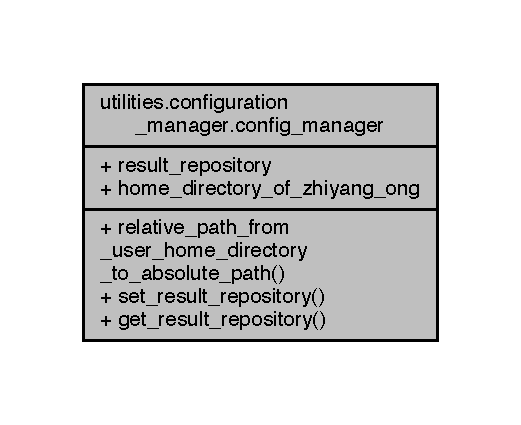
\includegraphics[width=250pt]{dc/d57/classutilities_1_1configuration__manager_1_1config__manager__coll__graph}
\end{center}
\end{figure}
\subsection*{Static Public Member Functions}
\begin{DoxyCompactItemize}
\item 
def \hyperlink{classutilities_1_1configuration__manager_1_1config__manager_a15f03ca784cab4d34b95dc020f3b0c23}{relative\+\_\+path\+\_\+from\+\_\+user\+\_\+home\+\_\+directory\+\_\+to\+\_\+absolute\+\_\+path} (location)
\begin{DoxyCompactList}\small\item\em Method to set the location of simulation/experimental results. \end{DoxyCompactList}\item 
def \hyperlink{classutilities_1_1configuration__manager_1_1config__manager_a3ac8c649652805fc0bddd2b6d8187329}{set\+\_\+result\+\_\+repository} (location)
\begin{DoxyCompactList}\small\item\em Method to set the location of simulation/experimental results. \end{DoxyCompactList}\item 
def \hyperlink{classutilities_1_1configuration__manager_1_1config__manager_a3e06a71db0338806c87430dc45fbab66}{get\+\_\+result\+\_\+repository} ()
\begin{DoxyCompactList}\small\item\em Method to get the location of simulation/experimental results. \end{DoxyCompactList}\end{DoxyCompactItemize}
\subsection*{Static Public Attributes}
\begin{DoxyCompactItemize}
\item 
string \hyperlink{classutilities_1_1configuration__manager_1_1config__manager_a19ed9ae453acea0ed85f704f18ee4b30}{result\+\_\+repository} = \char`\"{}Unknown location.\char`\"{}
\item 
string \hyperlink{classutilities_1_1configuration__manager_1_1config__manager_a884c4ec67676c35cc6fd674c208abfe2}{home\+\_\+directory\+\_\+of\+\_\+zhiyang\+\_\+ong} = \char`\"{}/Users/zhiyang\char`\"{}
\end{DoxyCompactItemize}


\subsection{Detailed Description}
Import Custom Python Modules. 

Module with methods that perform file I/\+O operations. 

Definition at line \hyperlink{configuration__manager_8py_source_l00088}{88} of file \hyperlink{configuration__manager_8py_source}{configuration\+\_\+manager.\+py}.



\subsection{Member Function Documentation}
\hypertarget{classutilities_1_1configuration__manager_1_1config__manager_a3e06a71db0338806c87430dc45fbab66}{}\index{utilities\+::configuration\+\_\+manager\+::config\+\_\+manager@{utilities\+::configuration\+\_\+manager\+::config\+\_\+manager}!get\+\_\+result\+\_\+repository@{get\+\_\+result\+\_\+repository}}
\index{get\+\_\+result\+\_\+repository@{get\+\_\+result\+\_\+repository}!utilities\+::configuration\+\_\+manager\+::config\+\_\+manager@{utilities\+::configuration\+\_\+manager\+::config\+\_\+manager}}
\subsubsection[{get\+\_\+result\+\_\+repository()}]{\setlength{\rightskip}{0pt plus 5cm}def utilities.\+configuration\+\_\+manager.\+config\+\_\+manager.\+get\+\_\+result\+\_\+repository (
\begin{DoxyParamCaption}
{}
\end{DoxyParamCaption}
)\hspace{0.3cm}{\ttfamily [static]}}\label{classutilities_1_1configuration__manager_1_1config__manager_a3e06a71db0338806c87430dc45fbab66}


Method to get the location of simulation/experimental results. 


\begin{DoxyParams}{Parameters}
{\em -\/} & None. \\
\hline
\end{DoxyParams}
\begin{DoxyReturn}{Returns}
the location of simulation/experimental results. O(1) method. 
\end{DoxyReturn}


Definition at line \hyperlink{configuration__manager_8py_source_l00163}{163} of file \hyperlink{configuration__manager_8py_source}{configuration\+\_\+manager.\+py}.


\begin{DoxyCode}
\hypertarget{classutilities_1_1configuration__manager_1_1config__manager_l00163}{}\hyperlink{classutilities_1_1configuration__manager_1_1config__manager_a3e06a71db0338806c87430dc45fbab66}{00163}     \textcolor{keyword}{def }\hyperlink{classutilities_1_1configuration__manager_1_1config__manager_a3e06a71db0338806c87430dc45fbab66}{get\_result\_repository}():
00164         \textcolor{keywordflow}{return} config\_manager.result\_repository
00165 \end{DoxyCode}
\hypertarget{classutilities_1_1configuration__manager_1_1config__manager_a15f03ca784cab4d34b95dc020f3b0c23}{}\index{utilities\+::configuration\+\_\+manager\+::config\+\_\+manager@{utilities\+::configuration\+\_\+manager\+::config\+\_\+manager}!relative\+\_\+path\+\_\+from\+\_\+user\+\_\+home\+\_\+directory\+\_\+to\+\_\+absolute\+\_\+path@{relative\+\_\+path\+\_\+from\+\_\+user\+\_\+home\+\_\+directory\+\_\+to\+\_\+absolute\+\_\+path}}
\index{relative\+\_\+path\+\_\+from\+\_\+user\+\_\+home\+\_\+directory\+\_\+to\+\_\+absolute\+\_\+path@{relative\+\_\+path\+\_\+from\+\_\+user\+\_\+home\+\_\+directory\+\_\+to\+\_\+absolute\+\_\+path}!utilities\+::configuration\+\_\+manager\+::config\+\_\+manager@{utilities\+::configuration\+\_\+manager\+::config\+\_\+manager}}
\subsubsection[{relative\+\_\+path\+\_\+from\+\_\+user\+\_\+home\+\_\+directory\+\_\+to\+\_\+absolute\+\_\+path(location)}]{\setlength{\rightskip}{0pt plus 5cm}def utilities.\+configuration\+\_\+manager.\+config\+\_\+manager.\+relative\+\_\+path\+\_\+from\+\_\+user\+\_\+home\+\_\+directory\+\_\+to\+\_\+absolute\+\_\+path (
\begin{DoxyParamCaption}
\item[{}]{location}
\end{DoxyParamCaption}
)\hspace{0.3cm}{\ttfamily [static]}}\label{classutilities_1_1configuration__manager_1_1config__manager_a15f03ca784cab4d34b95dc020f3b0c23}


Method to set the location of simulation/experimental results. 


\begin{DoxyParams}{Parameters}
{\em location} & -\/ Location of a directory. \\
\hline
\end{DoxyParams}
\begin{DoxyReturn}{Returns}
the absolute path of location, if location is a relative path from the user\textquotesingle{}s home directory. Else, return location. \subparagraph*{I\+M\+P\+O\+R\+T\+A\+N\+T N\+O\+T\+E\+S\+: Method to fix bug in the method}
\end{DoxyReturn}
\char`\"{}os.\+path.\+expanduser\char`\"{}, which had replaced the initial substring \char`\"{}$\sim$/\char`\"{} of the relative path from the user\textquotesingle{}s home directory with \char`\"{}../\char`\"{} This bug is not always replicable. This is because os.\+environ\mbox{[}\textquotesingle{}H\+O\+M\+E\textquotesingle{}\mbox{]} is set to \char`\"{}../\char`\"{}. Hence, it will replace \char`\"{}$\sim$/\char`\"{} with \char`\"{}../\char`\"{}. Hence, I am providing/using this workaround. O(1) method. 

Definition at line \hyperlink{configuration__manager_8py_source_l00110}{110} of file \hyperlink{configuration__manager_8py_source}{configuration\+\_\+manager.\+py}.


\begin{DoxyCode}
\hypertarget{classutilities_1_1configuration__manager_1_1config__manager_l00110}{}\hyperlink{classutilities_1_1configuration__manager_1_1config__manager_a15f03ca784cab4d34b95dc020f3b0c23}{00110}     \textcolor{keyword}{def }\hyperlink{classutilities_1_1configuration__manager_1_1config__manager_a15f03ca784cab4d34b95dc020f3b0c23}{relative\_path\_from\_user\_home\_directory\_to\_absolute\_path}
      (location):
00111         \textcolor{comment}{#print("Where is my home?",os.environ['HOME'],"=")}
00112         \textcolor{comment}{#home\_directory = os.path.expanduser("~")}
00113         \textcolor{comment}{#print("?   home\_directory:::",home\_directory,"=")}
00114         home\_directory\_of\_zhiyang\_ong = \textcolor{stringliteral}{"/Users/zhiyang/"}
00115         \textcolor{keywordflow}{if} location.startswith(\textcolor{stringliteral}{"~/"}):
00116             \textcolor{keywordflow}{return} location.replace(\textcolor{stringliteral}{"~/"},home\_directory\_of\_zhiyang\_ong)
00117         \textcolor{keywordflow}{else}:
00118             \textcolor{keywordflow}{return} location
\end{DoxyCode}
\hypertarget{classutilities_1_1configuration__manager_1_1config__manager_a3ac8c649652805fc0bddd2b6d8187329}{}\index{utilities\+::configuration\+\_\+manager\+::config\+\_\+manager@{utilities\+::configuration\+\_\+manager\+::config\+\_\+manager}!set\+\_\+result\+\_\+repository@{set\+\_\+result\+\_\+repository}}
\index{set\+\_\+result\+\_\+repository@{set\+\_\+result\+\_\+repository}!utilities\+::configuration\+\_\+manager\+::config\+\_\+manager@{utilities\+::configuration\+\_\+manager\+::config\+\_\+manager}}
\subsubsection[{set\+\_\+result\+\_\+repository(location)}]{\setlength{\rightskip}{0pt plus 5cm}def utilities.\+configuration\+\_\+manager.\+config\+\_\+manager.\+set\+\_\+result\+\_\+repository (
\begin{DoxyParamCaption}
\item[{}]{location}
\end{DoxyParamCaption}
)\hspace{0.3cm}{\ttfamily [static]}}\label{classutilities_1_1configuration__manager_1_1config__manager_a3ac8c649652805fc0bddd2b6d8187329}


Method to set the location of simulation/experimental results. 


\begin{DoxyParams}{Parameters}
{\em location} & -\/ Location of a directory. \\
\hline
\end{DoxyParams}
\begin{DoxyReturn}{Returns}
a boolean T\+R\+U\+E, if the location is a valid directory. Else, return F\+A\+L\+S\+E. O(1) method. \begin{DoxyVerb}    Since os.path.isdir returns false for relative paths,
ensure that the directory is an absolute path
    before proceeding.
\end{DoxyVerb}
 
\end{DoxyReturn}


Definition at line \hyperlink{configuration__manager_8py_source_l00126}{126} of file \hyperlink{configuration__manager_8py_source}{configuration\+\_\+manager.\+py}.


\begin{DoxyCode}
\hypertarget{classutilities_1_1configuration__manager_1_1config__manager_l00126}{}\hyperlink{classutilities_1_1configuration__manager_1_1config__manager_a3ac8c649652805fc0bddd2b6d8187329}{00126}     \textcolor{keyword}{def }\hyperlink{classutilities_1_1configuration__manager_1_1config__manager_a3ac8c649652805fc0bddd2b6d8187329}{set\_result\_repository}(location):
00127         \textcolor{stringliteral}{"""}
00128 \textcolor{stringliteral}{            Since os.path.isdir returns false for relative paths,}
00129 \textcolor{stringliteral}{                ensure that the directory is an absolute path}
00130 \textcolor{stringliteral}{                    before proceeding.}
00131 \textcolor{stringliteral}{        """}
00132         location = config\_manager.relative\_path\_from\_user\_home\_directory\_to\_absolute\_path(location)
00133         print(\textcolor{stringliteral}{";;;~current location:::"},location,\textcolor{stringliteral}{"="})
00134         \textcolor{keywordflow}{if} \textcolor{keywordflow}{not} os.path.isabs(location):
00135             \textcolor{comment}{#print("    location is a relative path.")}
00136             \textcolor{comment}{# Change the relative path to an absolute path.}
00137             location = os.path.expanduser(location)
00138             \textcolor{comment}{#print("    location made abs:::",location,"=")}
00139         print(\textcolor{stringliteral}{" location should be abs:::"},location,\textcolor{stringliteral}{"="})
00140         print(\textcolor{stringliteral}{"os.path.isdir(location)"},os.path.isdir(location),\textcolor{stringliteral}{"="})
00141         \textcolor{keywordflow}{if} os.path.isdir(location):
00142             config\_manager.result\_repository = location
00143             \textcolor{comment}{#print("config\_manager.result\_repository:::",config\_manager.result\_repository,"=")}
00144             \textcolor{comment}{#print("    config\_manager.result\_repository is set correctly.")}
00145             \textcolor{keywordflow}{return} \textcolor{keyword}{True}
00146         \textcolor{keywordflow}{else}:
00147             \textcolor{comment}{#print("    location is an invalid directory.")}
00148             \textcolor{comment}{#print("&&& config\_manager.result\_repository:::",config\_manager.result\_repository,"=")}
00149             \textcolor{comment}{#print("    'location' is a valid directory.")}
00150             \textcolor{comment}{#print("    'location' path
       check:::",os.path.isdir("/Users/zhiyang/Documents/ricerca/risultati\_sperimentali/std-cell-library-characterization"),"=")}
00151             \textcolor{comment}{#if "/Users/zhiyang/Documents/ricerca/risultati\_sperimentali/std-cell-library-characterization"
       == location.strip():}
00152             \textcolor{keywordflow}{if} \textcolor{stringliteral}{"/Users/zhiyang/Documents/ricerca/risultati\_sperimentali/std-cell-library-characterization"} 
      == location:
00153                 print(\textcolor{stringliteral}{"location value is WRONG!!!"})
00154             print(\textcolor{stringliteral}{" 'location':::"},location,\textcolor{stringliteral}{"="})
00155             \textcolor{comment}{#print("    'copy\_of\_location':::",copy\_of\_location,"=")}
00156             \textcolor{keywordflow}{return} \textcolor{keyword}{False}
\end{DoxyCode}


\subsection{Member Data Documentation}
\hypertarget{classutilities_1_1configuration__manager_1_1config__manager_a884c4ec67676c35cc6fd674c208abfe2}{}\index{utilities\+::configuration\+\_\+manager\+::config\+\_\+manager@{utilities\+::configuration\+\_\+manager\+::config\+\_\+manager}!home\+\_\+directory\+\_\+of\+\_\+zhiyang\+\_\+ong@{home\+\_\+directory\+\_\+of\+\_\+zhiyang\+\_\+ong}}
\index{home\+\_\+directory\+\_\+of\+\_\+zhiyang\+\_\+ong@{home\+\_\+directory\+\_\+of\+\_\+zhiyang\+\_\+ong}!utilities\+::configuration\+\_\+manager\+::config\+\_\+manager@{utilities\+::configuration\+\_\+manager\+::config\+\_\+manager}}
\subsubsection[{home\+\_\+directory\+\_\+of\+\_\+zhiyang\+\_\+ong}]{\setlength{\rightskip}{0pt plus 5cm}string utilities.\+configuration\+\_\+manager.\+config\+\_\+manager.\+home\+\_\+directory\+\_\+of\+\_\+zhiyang\+\_\+ong = \char`\"{}/Users/zhiyang\char`\"{}\hspace{0.3cm}{\ttfamily [static]}}\label{classutilities_1_1configuration__manager_1_1config__manager_a884c4ec67676c35cc6fd674c208abfe2}


Definition at line \hyperlink{configuration__manager_8py_source_l00092}{92} of file \hyperlink{configuration__manager_8py_source}{configuration\+\_\+manager.\+py}.

\hypertarget{classutilities_1_1configuration__manager_1_1config__manager_a19ed9ae453acea0ed85f704f18ee4b30}{}\index{utilities\+::configuration\+\_\+manager\+::config\+\_\+manager@{utilities\+::configuration\+\_\+manager\+::config\+\_\+manager}!result\+\_\+repository@{result\+\_\+repository}}
\index{result\+\_\+repository@{result\+\_\+repository}!utilities\+::configuration\+\_\+manager\+::config\+\_\+manager@{utilities\+::configuration\+\_\+manager\+::config\+\_\+manager}}
\subsubsection[{result\+\_\+repository}]{\setlength{\rightskip}{0pt plus 5cm}string utilities.\+configuration\+\_\+manager.\+config\+\_\+manager.\+result\+\_\+repository = \char`\"{}Unknown location.\char`\"{}\hspace{0.3cm}{\ttfamily [static]}}\label{classutilities_1_1configuration__manager_1_1config__manager_a19ed9ae453acea0ed85f704f18ee4b30}


Definition at line \hyperlink{configuration__manager_8py_source_l00091}{91} of file \hyperlink{configuration__manager_8py_source}{configuration\+\_\+manager.\+py}.



The documentation for this class was generated from the following file\+:\begin{DoxyCompactItemize}
\item 
utilities/\hyperlink{configuration__manager_8py}{configuration\+\_\+manager.\+py}\end{DoxyCompactItemize}

\hypertarget{classutilities_1_1configuration__manager__tester_1_1config__manager__tester}{}\section{utilities.\+configuration\+\_\+manager\+\_\+tester.\+config\+\_\+manager\+\_\+tester Class Reference}
\label{classutilities_1_1configuration__manager__tester_1_1config__manager__tester}\index{utilities.\+configuration\+\_\+manager\+\_\+tester.\+config\+\_\+manager\+\_\+tester@{utilities.\+configuration\+\_\+manager\+\_\+tester.\+config\+\_\+manager\+\_\+tester}}


Collaboration diagram for utilities.\+configuration\+\_\+manager\+\_\+tester.\+config\+\_\+manager\+\_\+tester\+:
\nopagebreak
\begin{figure}[H]
\begin{center}
\leavevmode

\includegraphics[width=238pt]{d4/dab/classutilities_1_1configuration__manager__tester_1_1config__manager__tester__coll__graph}
\end{center}
\end{figure}
\subsection*{Static Public Member Functions}
\begin{DoxyCompactItemize}
\item 
def \hyperlink{classutilities_1_1configuration__manager__tester_1_1config__manager__tester_a1f30cbc427332b33d4e4a8e32ae3b980}{test\+\_\+configure\+\_\+sw\+\_\+application\+\_\+parameters} ()
\begin{DoxyCompactList}\small\item\em ========================================================= Method to test the methods that configure the software application\textquotesingle{}s parameters. \end{DoxyCompactList}\end{DoxyCompactItemize}
\subsection*{Static Public Attributes}
\begin{DoxyCompactItemize}
\item 
string \hyperlink{classutilities_1_1configuration__manager__tester_1_1config__manager__tester_aa2904b10cd29c4fe16374fa249686be2}{prompt} = \char`\"{} ... Test\+: check default result\+\_\+repository \{\}\char`\"{}
\item 
string \hyperlink{classutilities_1_1configuration__manager__tester_1_1config__manager__tester_aa23d0c5b64043e706aa32519034a37e8}{absolute\+\_\+path} = \char`\"{}/Users/zhiyang/Documents/ricerca/risultati\+\_\+sperimentali/std-\/cell-\/library-\/characterization\char`\"{}
\end{DoxyCompactItemize}


\subsection{Detailed Description}


Definition at line \hyperlink{configuration__manager__tester_8py_source_l00092}{92} of file \hyperlink{configuration__manager__tester_8py_source}{configuration\+\_\+manager\+\_\+tester.\+py}.



\subsection{Member Function Documentation}
\hypertarget{classutilities_1_1configuration__manager__tester_1_1config__manager__tester_a1f30cbc427332b33d4e4a8e32ae3b980}{}\index{utilities\+::configuration\+\_\+manager\+\_\+tester\+::config\+\_\+manager\+\_\+tester@{utilities\+::configuration\+\_\+manager\+\_\+tester\+::config\+\_\+manager\+\_\+tester}!test\+\_\+configure\+\_\+sw\+\_\+application\+\_\+parameters@{test\+\_\+configure\+\_\+sw\+\_\+application\+\_\+parameters}}
\index{test\+\_\+configure\+\_\+sw\+\_\+application\+\_\+parameters@{test\+\_\+configure\+\_\+sw\+\_\+application\+\_\+parameters}!utilities\+::configuration\+\_\+manager\+\_\+tester\+::config\+\_\+manager\+\_\+tester@{utilities\+::configuration\+\_\+manager\+\_\+tester\+::config\+\_\+manager\+\_\+tester}}
\subsubsection[{test\+\_\+configure\+\_\+sw\+\_\+application\+\_\+parameters()}]{\setlength{\rightskip}{0pt plus 5cm}def utilities.\+configuration\+\_\+manager\+\_\+tester.\+config\+\_\+manager\+\_\+tester.\+test\+\_\+configure\+\_\+sw\+\_\+application\+\_\+parameters (
\begin{DoxyParamCaption}
{}
\end{DoxyParamCaption}
)\hspace{0.3cm}{\ttfamily [static]}}\label{classutilities_1_1configuration__manager__tester_1_1config__manager__tester_a1f30cbc427332b33d4e4a8e32ae3b980}


========================================================= Method to test the methods that configure the software application\textquotesingle{}s parameters. 


\begin{DoxyParams}{Parameters}
{\em -\/} & Nothing \\
\hline
\end{DoxyParams}
\begin{DoxyReturn}{Returns}
-\/ Nothing. O(1) method. 
\end{DoxyReturn}


Definition at line \hyperlink{configuration__manager__tester_8py_source_l00100}{100} of file \hyperlink{configuration__manager__tester_8py_source}{configuration\+\_\+manager\+\_\+tester.\+py}.


\begin{DoxyCode}
\hypertarget{classutilities_1_1configuration__manager__tester_1_1config__manager__tester_l00100}{}\hyperlink{classutilities_1_1configuration__manager__tester_1_1config__manager__tester_a1f30cbc427332b33d4e4a8e32ae3b980}{00100}     \textcolor{keyword}{def }\hyperlink{classutilities_1_1configuration__manager__tester_1_1config__manager__tester_a1f30cbc427332b33d4e4a8e32ae3b980}{test\_configure\_sw\_application\_parameters}():
\end{DoxyCode}


\subsection{Member Data Documentation}
\hypertarget{classutilities_1_1configuration__manager__tester_1_1config__manager__tester_aa23d0c5b64043e706aa32519034a37e8}{}\index{utilities\+::configuration\+\_\+manager\+\_\+tester\+::config\+\_\+manager\+\_\+tester@{utilities\+::configuration\+\_\+manager\+\_\+tester\+::config\+\_\+manager\+\_\+tester}!absolute\+\_\+path@{absolute\+\_\+path}}
\index{absolute\+\_\+path@{absolute\+\_\+path}!utilities\+::configuration\+\_\+manager\+\_\+tester\+::config\+\_\+manager\+\_\+tester@{utilities\+::configuration\+\_\+manager\+\_\+tester\+::config\+\_\+manager\+\_\+tester}}
\subsubsection[{absolute\+\_\+path}]{\setlength{\rightskip}{0pt plus 5cm}string utilities.\+configuration\+\_\+manager\+\_\+tester.\+config\+\_\+manager\+\_\+tester.\+absolute\+\_\+path = \char`\"{}/Users/zhiyang/Documents/ricerca/risultati\+\_\+sperimentali/std-\/cell-\/library-\/characterization\char`\"{}\hspace{0.3cm}{\ttfamily [static]}}\label{classutilities_1_1configuration__manager__tester_1_1config__manager__tester_aa23d0c5b64043e706aa32519034a37e8}


Definition at line \hyperlink{configuration__manager__tester_8py_source_l00113}{113} of file \hyperlink{configuration__manager__tester_8py_source}{configuration\+\_\+manager\+\_\+tester.\+py}.

\hypertarget{classutilities_1_1configuration__manager__tester_1_1config__manager__tester_aa2904b10cd29c4fe16374fa249686be2}{}\index{utilities\+::configuration\+\_\+manager\+\_\+tester\+::config\+\_\+manager\+\_\+tester@{utilities\+::configuration\+\_\+manager\+\_\+tester\+::config\+\_\+manager\+\_\+tester}!prompt@{prompt}}
\index{prompt@{prompt}!utilities\+::configuration\+\_\+manager\+\_\+tester\+::config\+\_\+manager\+\_\+tester@{utilities\+::configuration\+\_\+manager\+\_\+tester\+::config\+\_\+manager\+\_\+tester}}
\subsubsection[{prompt}]{\setlength{\rightskip}{0pt plus 5cm}string utilities.\+configuration\+\_\+manager\+\_\+tester.\+config\+\_\+manager\+\_\+tester.\+prompt = \char`\"{} ... Test\+: check default result\+\_\+repository \{\}\char`\"{}\hspace{0.3cm}{\ttfamily [static]}}\label{classutilities_1_1configuration__manager__tester_1_1config__manager__tester_aa2904b10cd29c4fe16374fa249686be2}
\begin{DoxyVerb}    Set "result_repository" to a relative path that is equivalent
absolute path, "absolute_path".
\end{DoxyVerb}
\begin{DoxyVerb}    "result_repository" is changed to an relative path.
    However, compare "result_repository" to the equivalent
absolute path.
    This is because if a relative path is detected, it will be
transform/changed to an absolute path, before being
assigned to "result_repository".
\end{DoxyVerb}
 

Definition at line \hyperlink{configuration__manager__tester_8py_source_l00105}{105} of file \hyperlink{configuration__manager__tester_8py_source}{configuration\+\_\+manager\+\_\+tester.\+py}.



The documentation for this class was generated from the following file\+:\begin{DoxyCompactItemize}
\item 
utilities/\hyperlink{configuration__manager__tester_8py}{configuration\+\_\+manager\+\_\+tester.\+py}\end{DoxyCompactItemize}

\hypertarget{classstatistics_1_1data__analysis__tool_1_1data__analysis}{}\section{statistics.\+data\+\_\+analysis\+\_\+tool.\+data\+\_\+analysis Class Reference}
\label{classstatistics_1_1data__analysis__tool_1_1data__analysis}\index{statistics.\+data\+\_\+analysis\+\_\+tool.\+data\+\_\+analysis@{statistics.\+data\+\_\+analysis\+\_\+tool.\+data\+\_\+analysis}}


Import Custom Python Modules.  




Collaboration diagram for statistics.\+data\+\_\+analysis\+\_\+tool.\+data\+\_\+analysis\+:
\nopagebreak
\begin{figure}[H]
\begin{center}
\leavevmode

\includegraphics[width=220pt]{db/da4/classstatistics_1_1data__analysis__tool_1_1data__analysis__coll__graph}
\end{center}
\end{figure}
\subsection*{Static Public Member Functions}
\begin{DoxyCompactItemize}
\item 
def \hyperlink{classstatistics_1_1data__analysis__tool_1_1data__analysis_a890a06cfd5f3dbb95a7d5e41ec89b8e9}{get\+\_\+reference\+\_\+value}
\item 
def \hyperlink{classstatistics_1_1data__analysis__tool_1_1data__analysis_a2559796fe2b8c7a1619e741345ff2f8d}{get\+\_\+actual\+\_\+change}
\item 
def \hyperlink{classstatistics_1_1data__analysis__tool_1_1data__analysis_a4443b2fd70b1f2632cc3e003915af2f3}{get\+\_\+absolute\+\_\+difference}
\item 
def \hyperlink{classstatistics_1_1data__analysis__tool_1_1data__analysis_a9a050987fc4c731a48d99a8db1e28c8c}{get\+\_\+relative\+\_\+change}
\item 
def \hyperlink{classstatistics_1_1data__analysis__tool_1_1data__analysis_ae013c86ec44948a2b9ac2798bd4a9cb2}{get\+\_\+percentage\+\_\+change}
\item 
def \hyperlink{classstatistics_1_1data__analysis__tool_1_1data__analysis_aac1f458b15db107e27de367591361884}{get\+\_\+relative\+\_\+error}
\item 
def \hyperlink{classstatistics_1_1data__analysis__tool_1_1data__analysis_a2c0e62016c7d45cc39b71372ccb6d028}{get\+\_\+percent\+\_\+error}
\item 
def \hyperlink{classstatistics_1_1data__analysis__tool_1_1data__analysis_a3eb98f0cd57564ad42dd8b2cef5feab5}{get\+\_\+arithmetic\+\_\+average\+\_\+of\+\_\+absolute\+\_\+values}
\item 
def \hyperlink{classstatistics_1_1data__analysis__tool_1_1data__analysis_a04973a814dd603d6603da8c4d21ea1d8}{get\+\_\+relative\+\_\+difference}
\end{DoxyCompactItemize}
\subsection*{Static Public Attributes}
\begin{DoxyCompactItemize}
\item 
dictionary \hyperlink{classstatistics_1_1data__analysis__tool_1_1data__analysis_a946ccd65157a8c3b3b9be607fcaed9f6}{dict\+\_\+of\+\_\+reference\+\_\+values} = \{\char`\"{}c\char`\"{}\+:299792458, \char`\"{}standard acceleration due to gravity\char`\"{}\+:9.\+80665, \char`\"{}standard atmosphere\char`\"{}\+:101325\}
\end{DoxyCompactItemize}


\subsection{Detailed Description}
Import Custom Python Modules. 

Definition at line \hyperlink{data__analysis__tool_8py_source_l00137}{137} of file \hyperlink{data__analysis__tool_8py_source}{data\+\_\+analysis\+\_\+tool.\+py}.



\subsection{Member Function Documentation}
\hypertarget{classstatistics_1_1data__analysis__tool_1_1data__analysis_a4443b2fd70b1f2632cc3e003915af2f3}{}\index{statistics\+::data\+\_\+analysis\+\_\+tool\+::data\+\_\+analysis@{statistics\+::data\+\_\+analysis\+\_\+tool\+::data\+\_\+analysis}!get\+\_\+absolute\+\_\+difference@{get\+\_\+absolute\+\_\+difference}}
\index{get\+\_\+absolute\+\_\+difference@{get\+\_\+absolute\+\_\+difference}!statistics\+::data\+\_\+analysis\+\_\+tool\+::data\+\_\+analysis@{statistics\+::data\+\_\+analysis\+\_\+tool\+::data\+\_\+analysis}}
\subsubsection[{get\+\_\+absolute\+\_\+difference}]{\setlength{\rightskip}{0pt plus 5cm}def statistics.\+data\+\_\+analysis\+\_\+tool.\+data\+\_\+analysis.\+get\+\_\+absolute\+\_\+difference (
\begin{DoxyParamCaption}
\item[{}]{quantity1 = {\ttfamily 0}, }
\item[{}]{quantity2 = {\ttfamily 0}}
\end{DoxyParamCaption}
)\hspace{0.3cm}{\ttfamily [static]}}\label{classstatistics_1_1data__analysis__tool_1_1data__analysis_a4443b2fd70b1f2632cc3e003915af2f3}
\begin{DoxyVerb}    Check postcondition:
absolute difference, |quantity1 - quantity2| >= 0.
\end{DoxyVerb}
 

Definition at line \hyperlink{data__analysis__tool_8py_source_l00189}{189} of file \hyperlink{data__analysis__tool_8py_source}{data\+\_\+analysis\+\_\+tool.\+py}.


\begin{DoxyCode}
\hypertarget{classstatistics_1_1data__analysis__tool_1_1data__analysis_l00189}{}\hyperlink{classstatistics_1_1data__analysis__tool_1_1data__analysis_a4443b2fd70b1f2632cc3e003915af2f3}{00189}     \textcolor{keyword}{def }\hyperlink{classstatistics_1_1data__analysis__tool_1_1data__analysis_a4443b2fd70b1f2632cc3e003915af2f3}{get\_absolute\_difference}(quantity1=0,quantity2=0):
00190         \textcolor{stringliteral}{"""}
00191 \textcolor{stringliteral}{            Check postcondition:}
00192 \textcolor{stringliteral}{                absolute difference, |quantity1 - quantity2| >= 0.}
00193 \textcolor{stringliteral}{        """}
00194         absolute\_difference = abs(quantity1 - quantity2)
00195         \textcolor{keywordflow}{if} (0 > absolute\_difference):
00196             \textcolor{keywordflow}{raise} Exception(\textcolor{stringliteral}{"   get\_absolute\_difference(): Absolute difference must be non-negative."})
00197         \textcolor{keywordflow}{return} absolute\_difference
\end{DoxyCode}
\hypertarget{classstatistics_1_1data__analysis__tool_1_1data__analysis_a2559796fe2b8c7a1619e741345ff2f8d}{}\index{statistics\+::data\+\_\+analysis\+\_\+tool\+::data\+\_\+analysis@{statistics\+::data\+\_\+analysis\+\_\+tool\+::data\+\_\+analysis}!get\+\_\+actual\+\_\+change@{get\+\_\+actual\+\_\+change}}
\index{get\+\_\+actual\+\_\+change@{get\+\_\+actual\+\_\+change}!statistics\+::data\+\_\+analysis\+\_\+tool\+::data\+\_\+analysis@{statistics\+::data\+\_\+analysis\+\_\+tool\+::data\+\_\+analysis}}
\subsubsection[{get\+\_\+actual\+\_\+change}]{\setlength{\rightskip}{0pt plus 5cm}def statistics.\+data\+\_\+analysis\+\_\+tool.\+data\+\_\+analysis.\+get\+\_\+actual\+\_\+change (
\begin{DoxyParamCaption}
\item[{}]{quantity1 = {\ttfamily 0}, }
\item[{}]{quantity2 = {\ttfamily 0}}
\end{DoxyParamCaption}
)\hspace{0.3cm}{\ttfamily [static]}}\label{classstatistics_1_1data__analysis__tool_1_1data__analysis_a2559796fe2b8c7a1619e741345ff2f8d}


Definition at line \hyperlink{data__analysis__tool_8py_source_l00173}{173} of file \hyperlink{data__analysis__tool_8py_source}{data\+\_\+analysis\+\_\+tool.\+py}.


\begin{DoxyCode}
\hypertarget{classstatistics_1_1data__analysis__tool_1_1data__analysis_l00173}{}\hyperlink{classstatistics_1_1data__analysis__tool_1_1data__analysis_a2559796fe2b8c7a1619e741345ff2f8d}{00173}     \textcolor{keyword}{def }\hyperlink{classstatistics_1_1data__analysis__tool_1_1data__analysis_a2559796fe2b8c7a1619e741345ff2f8d}{get\_actual\_change}(quantity1=0,quantity2=0):
00174         \textcolor{keywordflow}{return} (quantity1 - quantity2)
\end{DoxyCode}
\hypertarget{classstatistics_1_1data__analysis__tool_1_1data__analysis_a3eb98f0cd57564ad42dd8b2cef5feab5}{}\index{statistics\+::data\+\_\+analysis\+\_\+tool\+::data\+\_\+analysis@{statistics\+::data\+\_\+analysis\+\_\+tool\+::data\+\_\+analysis}!get\+\_\+arithmetic\+\_\+average\+\_\+of\+\_\+absolute\+\_\+values@{get\+\_\+arithmetic\+\_\+average\+\_\+of\+\_\+absolute\+\_\+values}}
\index{get\+\_\+arithmetic\+\_\+average\+\_\+of\+\_\+absolute\+\_\+values@{get\+\_\+arithmetic\+\_\+average\+\_\+of\+\_\+absolute\+\_\+values}!statistics\+::data\+\_\+analysis\+\_\+tool\+::data\+\_\+analysis@{statistics\+::data\+\_\+analysis\+\_\+tool\+::data\+\_\+analysis}}
\subsubsection[{get\+\_\+arithmetic\+\_\+average\+\_\+of\+\_\+absolute\+\_\+values}]{\setlength{\rightskip}{0pt plus 5cm}def statistics.\+data\+\_\+analysis\+\_\+tool.\+data\+\_\+analysis.\+get\+\_\+arithmetic\+\_\+average\+\_\+of\+\_\+absolute\+\_\+values (
\begin{DoxyParamCaption}
\item[{}]{list\+\_\+of\+\_\+numbers = {\ttfamily \mbox{[}\mbox{]}}}
\end{DoxyParamCaption}
)\hspace{0.3cm}{\ttfamily [static]}}\label{classstatistics_1_1data__analysis__tool_1_1data__analysis_a3eb98f0cd57564ad42dd8b2cef5feab5}


Definition at line \hyperlink{data__analysis__tool_8py_source_l00284}{284} of file \hyperlink{data__analysis__tool_8py_source}{data\+\_\+analysis\+\_\+tool.\+py}.



Referenced by \hyperlink{data__analysis__tool_8py_source_l00324}{statistics.\+data\+\_\+analysis\+\_\+tool.\+data\+\_\+analysis.\+get\+\_\+relative\+\_\+difference()}.


\begin{DoxyCode}
\hypertarget{classstatistics_1_1data__analysis__tool_1_1data__analysis_l00284}{}\hyperlink{classstatistics_1_1data__analysis__tool_1_1data__analysis_a3eb98f0cd57564ad42dd8b2cef5feab5}{00284}     \textcolor{keyword}{def }\hyperlink{classstatistics_1_1data__analysis__tool_1_1data__analysis_a3eb98f0cd57564ad42dd8b2cef5feab5}{get\_arithmetic\_average\_of\_absolute\_values}(
      list\_of\_numbers=[]):
00285         \textcolor{comment}{# Check precondition: list\_of\_numbers is not a None object.}
00286         \textcolor{keywordflow}{if} list\_of\_numbers \textcolor{keywordflow}{is} \textcolor{keywordtype}{None}:
00287             \textcolor{keywordflow}{raise} Exception(\textcolor{stringliteral}{"   A 'None' object is passed to the
       get\_arithmetic\_average\_of\_absolute\_values() method."})
00288         \textcolor{comment}{# Else, is list\_of\_numbers an empty list?}
00289         \textcolor{comment}{#elif 0 == len(list\_of\_numbers):}
00290         \textcolor{keywordflow}{elif} \textcolor{keywordflow}{not} list\_of\_numbers:   \textcolor{comment}{# More Pythonic solution.}
00291             \textcolor{keywordflow}{return} 0
00292         \textcolor{keywordflow}{else}:
00293             \textcolor{stringliteral}{"""}
00294 \textcolor{stringliteral}{                Copy the absolute values of numbers in the list to}
00295 \textcolor{stringliteral}{                    another list, absolute\_list\_of\_numbers.}
00296 \textcolor{stringliteral}{            """}
00297             absolute\_list\_of\_numbers = []
00298             \textcolor{keywordflow}{for} elem \textcolor{keywordflow}{in} list\_of\_numbers:
00299                 absolute\_list\_of\_numbers.append(abs(elem))
00300             \textcolor{comment}{#print("absolute\_list\_of\_numbers:",absolute\_list\_of\_numbers,"=")}
00301             \textcolor{comment}{# Determine the arithmetic mean of these absolute values.}
00302             mean\_absolute\_list\_of\_numbers = s.mean(absolute\_list\_of\_numbers)
00303             \textcolor{comment}{# Check postcondition: mean of absolute values of numbers >= 0.}
00304             \textcolor{keywordflow}{if} 0 > mean\_absolute\_list\_of\_numbers:
00305                 \textcolor{keywordflow}{raise} Exception(\textcolor{stringliteral}{"   mean of the list of absolute values. < 0."})
00306             \textcolor{keywordflow}{return} mean\_absolute\_list\_of\_numbers
\end{DoxyCode}


Here is the caller graph for this function\+:
\nopagebreak
\begin{figure}[H]
\begin{center}
\leavevmode
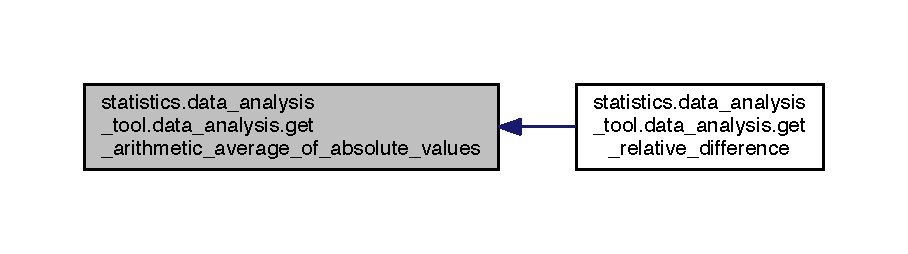
\includegraphics[width=350pt]{d8/dd7/classstatistics_1_1data__analysis__tool_1_1data__analysis_a3eb98f0cd57564ad42dd8b2cef5feab5_icgraph}
\end{center}
\end{figure}


\hypertarget{classstatistics_1_1data__analysis__tool_1_1data__analysis_a2c0e62016c7d45cc39b71372ccb6d028}{}\index{statistics\+::data\+\_\+analysis\+\_\+tool\+::data\+\_\+analysis@{statistics\+::data\+\_\+analysis\+\_\+tool\+::data\+\_\+analysis}!get\+\_\+percent\+\_\+error@{get\+\_\+percent\+\_\+error}}
\index{get\+\_\+percent\+\_\+error@{get\+\_\+percent\+\_\+error}!statistics\+::data\+\_\+analysis\+\_\+tool\+::data\+\_\+analysis@{statistics\+::data\+\_\+analysis\+\_\+tool\+::data\+\_\+analysis}}
\subsubsection[{get\+\_\+percent\+\_\+error}]{\setlength{\rightskip}{0pt plus 5cm}def statistics.\+data\+\_\+analysis\+\_\+tool.\+data\+\_\+analysis.\+get\+\_\+percent\+\_\+error (
\begin{DoxyParamCaption}
\item[{}]{experimental\+\_\+value = {\ttfamily 1}, }
\item[{}]{theoretical\+\_\+value = {\ttfamily 1}}
\end{DoxyParamCaption}
)\hspace{0.3cm}{\ttfamily [static]}}\label{classstatistics_1_1data__analysis__tool_1_1data__analysis_a2c0e62016c7d45cc39b71372ccb6d028}


Definition at line \hyperlink{data__analysis__tool_8py_source_l00261}{261} of file \hyperlink{data__analysis__tool_8py_source}{data\+\_\+analysis\+\_\+tool.\+py}.


\begin{DoxyCode}
\hypertarget{classstatistics_1_1data__analysis__tool_1_1data__analysis_l00261}{}\hyperlink{classstatistics_1_1data__analysis__tool_1_1data__analysis_a2c0e62016c7d45cc39b71372ccb6d028}{00261}     \textcolor{keyword}{def }\hyperlink{classstatistics_1_1data__analysis__tool_1_1data__analysis_a2c0e62016c7d45cc39b71372ccb6d028}{get\_percent\_error}(experimental\_value=1,theoretical\_value=1):
00262         \textcolor{keywordflow}{return} (data\_analysis.get\_relative\_error(experimental\_value,theoretical\_value)*100)
\end{DoxyCode}
\hypertarget{classstatistics_1_1data__analysis__tool_1_1data__analysis_ae013c86ec44948a2b9ac2798bd4a9cb2}{}\index{statistics\+::data\+\_\+analysis\+\_\+tool\+::data\+\_\+analysis@{statistics\+::data\+\_\+analysis\+\_\+tool\+::data\+\_\+analysis}!get\+\_\+percentage\+\_\+change@{get\+\_\+percentage\+\_\+change}}
\index{get\+\_\+percentage\+\_\+change@{get\+\_\+percentage\+\_\+change}!statistics\+::data\+\_\+analysis\+\_\+tool\+::data\+\_\+analysis@{statistics\+::data\+\_\+analysis\+\_\+tool\+::data\+\_\+analysis}}
\subsubsection[{get\+\_\+percentage\+\_\+change}]{\setlength{\rightskip}{0pt plus 5cm}def statistics.\+data\+\_\+analysis\+\_\+tool.\+data\+\_\+analysis.\+get\+\_\+percentage\+\_\+change (
\begin{DoxyParamCaption}
\item[{}]{quantity1 = {\ttfamily 1}, }
\item[{}]{ref\+\_\+qty = {\ttfamily 1}}
\end{DoxyParamCaption}
)\hspace{0.3cm}{\ttfamily [static]}}\label{classstatistics_1_1data__analysis__tool_1_1data__analysis_ae013c86ec44948a2b9ac2798bd4a9cb2}


Definition at line \hyperlink{data__analysis__tool_8py_source_l00229}{229} of file \hyperlink{data__analysis__tool_8py_source}{data\+\_\+analysis\+\_\+tool.\+py}.


\begin{DoxyCode}
\hypertarget{classstatistics_1_1data__analysis__tool_1_1data__analysis_l00229}{}\hyperlink{classstatistics_1_1data__analysis__tool_1_1data__analysis_ae013c86ec44948a2b9ac2798bd4a9cb2}{00229}     \textcolor{keyword}{def }\hyperlink{classstatistics_1_1data__analysis__tool_1_1data__analysis_ae013c86ec44948a2b9ac2798bd4a9cb2}{get\_percentage\_change}(quantity1=1,ref\_qty=1):
00230         \textcolor{comment}{# Check precondition: ref\_qty != 0.}
00231         \textcolor{keywordflow}{if} 0 == ref\_qty:
00232             \textcolor{keywordflow}{raise} Exception(\textcolor{stringliteral}{"   ref\_qty cannot be zero."})
00233         relative\_change = data\_analysis.get\_relative\_change(quantity1,ref\_qty)
00234         \textcolor{keywordflow}{return} (relative\_change*100)
\end{DoxyCode}
\hypertarget{classstatistics_1_1data__analysis__tool_1_1data__analysis_a890a06cfd5f3dbb95a7d5e41ec89b8e9}{}\index{statistics\+::data\+\_\+analysis\+\_\+tool\+::data\+\_\+analysis@{statistics\+::data\+\_\+analysis\+\_\+tool\+::data\+\_\+analysis}!get\+\_\+reference\+\_\+value@{get\+\_\+reference\+\_\+value}}
\index{get\+\_\+reference\+\_\+value@{get\+\_\+reference\+\_\+value}!statistics\+::data\+\_\+analysis\+\_\+tool\+::data\+\_\+analysis@{statistics\+::data\+\_\+analysis\+\_\+tool\+::data\+\_\+analysis}}
\subsubsection[{get\+\_\+reference\+\_\+value}]{\setlength{\rightskip}{0pt plus 5cm}def statistics.\+data\+\_\+analysis\+\_\+tool.\+data\+\_\+analysis.\+get\+\_\+reference\+\_\+value (
\begin{DoxyParamCaption}
\item[{}]{property = {\ttfamily \char`\"{}c\char`\"{}}}
\end{DoxyParamCaption}
)\hspace{0.3cm}{\ttfamily [static]}}\label{classstatistics_1_1data__analysis__tool_1_1data__analysis_a890a06cfd5f3dbb95a7d5e41ec89b8e9}


Definition at line \hyperlink{data__analysis__tool_8py_source_l00159}{159} of file \hyperlink{data__analysis__tool_8py_source}{data\+\_\+analysis\+\_\+tool.\+py}.


\begin{DoxyCode}
\hypertarget{classstatistics_1_1data__analysis__tool_1_1data__analysis_l00159}{}\hyperlink{classstatistics_1_1data__analysis__tool_1_1data__analysis_a890a06cfd5f3dbb95a7d5e41ec89b8e9}{00159}     \textcolor{keyword}{def }\hyperlink{classstatistics_1_1data__analysis__tool_1_1data__analysis_a890a06cfd5f3dbb95a7d5e41ec89b8e9}{get\_reference\_value}(property="c"):
00160         \textcolor{keywordflow}{return} data\_analysis.dict\_of\_reference\_values[property]
\end{DoxyCode}
\hypertarget{classstatistics_1_1data__analysis__tool_1_1data__analysis_a9a050987fc4c731a48d99a8db1e28c8c}{}\index{statistics\+::data\+\_\+analysis\+\_\+tool\+::data\+\_\+analysis@{statistics\+::data\+\_\+analysis\+\_\+tool\+::data\+\_\+analysis}!get\+\_\+relative\+\_\+change@{get\+\_\+relative\+\_\+change}}
\index{get\+\_\+relative\+\_\+change@{get\+\_\+relative\+\_\+change}!statistics\+::data\+\_\+analysis\+\_\+tool\+::data\+\_\+analysis@{statistics\+::data\+\_\+analysis\+\_\+tool\+::data\+\_\+analysis}}
\subsubsection[{get\+\_\+relative\+\_\+change}]{\setlength{\rightskip}{0pt plus 5cm}def statistics.\+data\+\_\+analysis\+\_\+tool.\+data\+\_\+analysis.\+get\+\_\+relative\+\_\+change (
\begin{DoxyParamCaption}
\item[{}]{quantity1 = {\ttfamily 1}, }
\item[{}]{ref\+\_\+qty = {\ttfamily 1}}
\end{DoxyParamCaption}
)\hspace{0.3cm}{\ttfamily [static]}}\label{classstatistics_1_1data__analysis__tool_1_1data__analysis_a9a050987fc4c731a48d99a8db1e28c8c}


Definition at line \hyperlink{data__analysis__tool_8py_source_l00211}{211} of file \hyperlink{data__analysis__tool_8py_source}{data\+\_\+analysis\+\_\+tool.\+py}.


\begin{DoxyCode}
\hypertarget{classstatistics_1_1data__analysis__tool_1_1data__analysis_l00211}{}\hyperlink{classstatistics_1_1data__analysis__tool_1_1data__analysis_a9a050987fc4c731a48d99a8db1e28c8c}{00211}     \textcolor{keyword}{def }\hyperlink{classstatistics_1_1data__analysis__tool_1_1data__analysis_a9a050987fc4c731a48d99a8db1e28c8c}{get\_relative\_change}(quantity1=1,ref\_qty=1):
00212         \textcolor{comment}{# Check precondition: ref\_qty != 0.}
00213         \textcolor{keywordflow}{if} 0 == ref\_qty:
00214             \textcolor{keywordflow}{raise} Exception(\textcolor{stringliteral}{"   ref\_qty cannot be zero."})
00215         \textcolor{keywordflow}{return} (data\_analysis.get\_actual\_change(quantity1,ref\_qty)/ref\_qty)
\end{DoxyCode}
\hypertarget{classstatistics_1_1data__analysis__tool_1_1data__analysis_a04973a814dd603d6603da8c4d21ea1d8}{}\index{statistics\+::data\+\_\+analysis\+\_\+tool\+::data\+\_\+analysis@{statistics\+::data\+\_\+analysis\+\_\+tool\+::data\+\_\+analysis}!get\+\_\+relative\+\_\+difference@{get\+\_\+relative\+\_\+difference}}
\index{get\+\_\+relative\+\_\+difference@{get\+\_\+relative\+\_\+difference}!statistics\+::data\+\_\+analysis\+\_\+tool\+::data\+\_\+analysis@{statistics\+::data\+\_\+analysis\+\_\+tool\+::data\+\_\+analysis}}
\subsubsection[{get\+\_\+relative\+\_\+difference}]{\setlength{\rightskip}{0pt plus 5cm}def statistics.\+data\+\_\+analysis\+\_\+tool.\+data\+\_\+analysis.\+get\+\_\+relative\+\_\+difference (
\begin{DoxyParamCaption}
\item[{}]{quantity1 = {\ttfamily 1}, }
\item[{}]{quantity2 = {\ttfamily 1}}
\end{DoxyParamCaption}
)\hspace{0.3cm}{\ttfamily [static]}}\label{classstatistics_1_1data__analysis__tool_1_1data__analysis_a04973a814dd603d6603da8c4d21ea1d8}


Definition at line \hyperlink{data__analysis__tool_8py_source_l00324}{324} of file \hyperlink{data__analysis__tool_8py_source}{data\+\_\+analysis\+\_\+tool.\+py}.



References \hyperlink{data__analysis__tool_8py_source_l00284}{statistics.\+data\+\_\+analysis\+\_\+tool.\+data\+\_\+analysis.\+get\+\_\+arithmetic\+\_\+average\+\_\+of\+\_\+absolute\+\_\+values()}.


\begin{DoxyCode}
\hypertarget{classstatistics_1_1data__analysis__tool_1_1data__analysis_l00324}{}\hyperlink{classstatistics_1_1data__analysis__tool_1_1data__analysis_a04973a814dd603d6603da8c4d21ea1d8}{00324}     \textcolor{keyword}{def }\hyperlink{classstatistics_1_1data__analysis__tool_1_1data__analysis_a04973a814dd603d6603da8c4d21ea1d8}{get\_relative\_difference}(quantity1=1,quantity2=1):
00325         \textcolor{comment}{# Check for precondition: (quantity1 != 0) or (quantity2 != 0).}
00326         \textcolor{keywordflow}{if} (0 == quantity1) \textcolor{keywordflow}{and} (0 == quantity2):
00327             \textcolor{keywordflow}{raise} Exception(\textcolor{stringliteral}{"   relative difference does not exist for quantity1 == quantity2."})
00328         absolute\_diff = data\_analysis.get\_absolute\_difference(quantity1,quantity2)
00329         \textcolor{comment}{# Check assertion: absolute difference, |quantity1 - quantity2| >= 0.}
00330         \textcolor{keywordflow}{if} 0 > absolute\_diff:
00331             \textcolor{keywordflow}{raise} Exception(\textcolor{stringliteral}{"   get\_relative\_difference(): Absolute difference must be non-negative."})
00332         list\_of\_values = [quantity1, quantity2]
00333         average\_of\_absolute\_values = \hyperlink{classstatistics_1_1data__analysis__tool_1_1data__analysis_a3eb98f0cd57564ad42dd8b2cef5feab5}{get\_arithmetic\_average\_of\_absolute\_values}
      (list\_of\_numbers)
00334         \textcolor{comment}{# Check postcondition: average\_of\_absolute\_values > 0.}
00335         \textcolor{keywordflow}{if} 0 >= average\_of\_absolute\_values:
00336             \textcolor{keywordflow}{raise} Exception(\textcolor{stringliteral}{"   0 >= arithmetic mean of absolute values."})
00337         \textcolor{keywordflow}{return} (absolute\_diff/average\_of\_absolute\_values)
00338     
00339 \end{DoxyCode}


Here is the call graph for this function\+:
\nopagebreak
\begin{figure}[H]
\begin{center}
\leavevmode

\includegraphics[width=350pt]{d8/dd7/classstatistics_1_1data__analysis__tool_1_1data__analysis_a04973a814dd603d6603da8c4d21ea1d8_cgraph}
\end{center}
\end{figure}


\hypertarget{classstatistics_1_1data__analysis__tool_1_1data__analysis_aac1f458b15db107e27de367591361884}{}\index{statistics\+::data\+\_\+analysis\+\_\+tool\+::data\+\_\+analysis@{statistics\+::data\+\_\+analysis\+\_\+tool\+::data\+\_\+analysis}!get\+\_\+relative\+\_\+error@{get\+\_\+relative\+\_\+error}}
\index{get\+\_\+relative\+\_\+error@{get\+\_\+relative\+\_\+error}!statistics\+::data\+\_\+analysis\+\_\+tool\+::data\+\_\+analysis@{statistics\+::data\+\_\+analysis\+\_\+tool\+::data\+\_\+analysis}}
\subsubsection[{get\+\_\+relative\+\_\+error}]{\setlength{\rightskip}{0pt plus 5cm}def statistics.\+data\+\_\+analysis\+\_\+tool.\+data\+\_\+analysis.\+get\+\_\+relative\+\_\+error (
\begin{DoxyParamCaption}
\item[{}]{experimental\+\_\+value = {\ttfamily 1}, }
\item[{}]{theoretical\+\_\+value = {\ttfamily 1}}
\end{DoxyParamCaption}
)\hspace{0.3cm}{\ttfamily [static]}}\label{classstatistics_1_1data__analysis__tool_1_1data__analysis_aac1f458b15db107e27de367591361884}


Definition at line \hyperlink{data__analysis__tool_8py_source_l00247}{247} of file \hyperlink{data__analysis__tool_8py_source}{data\+\_\+analysis\+\_\+tool.\+py}.


\begin{DoxyCode}
\hypertarget{classstatistics_1_1data__analysis__tool_1_1data__analysis_l00247}{}\hyperlink{classstatistics_1_1data__analysis__tool_1_1data__analysis_aac1f458b15db107e27de367591361884}{00247}     \textcolor{keyword}{def }\hyperlink{classstatistics_1_1data__analysis__tool_1_1data__analysis_aac1f458b15db107e27de367591361884}{get\_relative\_error}(experimental\_value=1,theoretical\_value=1):
00248         \textcolor{keywordflow}{return} (data\_analysis.get\_absolute\_difference(experimental\_value,theoretical\_value)/abs(
      theoretical\_value))
\end{DoxyCode}


\subsection{Member Data Documentation}
\hypertarget{classstatistics_1_1data__analysis__tool_1_1data__analysis_a946ccd65157a8c3b3b9be607fcaed9f6}{}\index{statistics\+::data\+\_\+analysis\+\_\+tool\+::data\+\_\+analysis@{statistics\+::data\+\_\+analysis\+\_\+tool\+::data\+\_\+analysis}!dict\+\_\+of\+\_\+reference\+\_\+values@{dict\+\_\+of\+\_\+reference\+\_\+values}}
\index{dict\+\_\+of\+\_\+reference\+\_\+values@{dict\+\_\+of\+\_\+reference\+\_\+values}!statistics\+::data\+\_\+analysis\+\_\+tool\+::data\+\_\+analysis@{statistics\+::data\+\_\+analysis\+\_\+tool\+::data\+\_\+analysis}}
\subsubsection[{dict\+\_\+of\+\_\+reference\+\_\+values}]{\setlength{\rightskip}{0pt plus 5cm}dictionary statistics.\+data\+\_\+analysis\+\_\+tool.\+data\+\_\+analysis.\+dict\+\_\+of\+\_\+reference\+\_\+values = \{\char`\"{}c\char`\"{}\+:299792458, \char`\"{}standard acceleration due to gravity\char`\"{}\+:9.\+80665, \char`\"{}standard atmosphere\char`\"{}\+:101325\}\hspace{0.3cm}{\ttfamily [static]}}\label{classstatistics_1_1data__analysis__tool_1_1data__analysis_a946ccd65157a8c3b3b9be607fcaed9f6}


Definition at line \hyperlink{data__analysis__tool_8py_source_l00151}{151} of file \hyperlink{data__analysis__tool_8py_source}{data\+\_\+analysis\+\_\+tool.\+py}.



The documentation for this class was generated from the following file\+:\begin{DoxyCompactItemize}
\item 
statistics/\hyperlink{data__analysis__tool_8py}{data\+\_\+analysis\+\_\+tool.\+py}\end{DoxyCompactItemize}

\hypertarget{classstatistics_1_1test__data__analysis__tool_1_1data__analysis__tester}{}\section{statistics.\+test\+\_\+data\+\_\+analysis\+\_\+tool.\+data\+\_\+analysis\+\_\+tester Class Reference}
\label{classstatistics_1_1test__data__analysis__tool_1_1data__analysis__tester}\index{statistics.\+test\+\_\+data\+\_\+analysis\+\_\+tool.\+data\+\_\+analysis\+\_\+tester@{statistics.\+test\+\_\+data\+\_\+analysis\+\_\+tool.\+data\+\_\+analysis\+\_\+tester}}


Collaboration diagram for statistics.\+test\+\_\+data\+\_\+analysis\+\_\+tool.\+data\+\_\+analysis\+\_\+tester\+:
\nopagebreak
\begin{figure}[H]
\begin{center}
\leavevmode

\includegraphics[width=240pt]{dc/d96/classstatistics_1_1test__data__analysis__tool_1_1data__analysis__tester__coll__graph}
\end{center}
\end{figure}
\subsection*{Static Public Member Functions}
\begin{DoxyCompactItemize}
\item 
def \hyperlink{classstatistics_1_1test__data__analysis__tool_1_1data__analysis__tester_ac5dee1d2f7bb003c3b322ec9692766af}{test\+\_\+get\+\_\+reference\+\_\+value} ()
\begin{DoxyCompactList}\small\item\em ========================================================= Method to test the method that accesses reference values for a corresponding particular attribute/property, using the Python dictionary containing pairs/2-\/tuples of attributes/properties and values. \end{DoxyCompactList}\item 
def \hyperlink{classstatistics_1_1test__data__analysis__tool_1_1data__analysis__tester_af355b89d75dbd6f03b47a52bcfdb9025}{test\+\_\+get\+\_\+actual\+\_\+change} ()
\begin{DoxyCompactList}\small\item\em ========================================================= Method to test the method that determines the actual change between quantity1 and quantity2. \end{DoxyCompactList}\item 
def \hyperlink{classstatistics_1_1test__data__analysis__tool_1_1data__analysis__tester_a3b1f6f4fd16ef986ead81484c80fc164}{test\+\_\+get\+\_\+absolute\+\_\+difference} ()
\begin{DoxyCompactList}\small\item\em ========================================================= Method to test the method that determines the absolute difference between quantity1 and quantity2. \end{DoxyCompactList}\item 
def \hyperlink{classstatistics_1_1test__data__analysis__tool_1_1data__analysis__tester_a8ca74240a173de29733a73137df4bd95}{test\+\_\+get\+\_\+relative\+\_\+change} ()
\begin{DoxyCompactList}\small\item\em ========================================================= Method to test the method that determines the relative change between quantity1 and quantity2. \end{DoxyCompactList}\item 
def \hyperlink{classstatistics_1_1test__data__analysis__tool_1_1data__analysis__tester_a770fcf75cc2e1a9e8e840d1f3bb770af}{test\+\_\+data\+\_\+analysis} ()
\begin{DoxyCompactList}\small\item\em Method to test the methods that perform miscellaneous tasks in data analysis. \end{DoxyCompactList}\end{DoxyCompactItemize}


\subsection{Detailed Description}


Definition at line \hyperlink{test__data__analysis__tool_8py_source_l00097}{97} of file \hyperlink{test__data__analysis__tool_8py_source}{test\+\_\+data\+\_\+analysis\+\_\+tool.\+py}.



\subsection{Member Function Documentation}
\hypertarget{classstatistics_1_1test__data__analysis__tool_1_1data__analysis__tester_a770fcf75cc2e1a9e8e840d1f3bb770af}{}\index{statistics\+::test\+\_\+data\+\_\+analysis\+\_\+tool\+::data\+\_\+analysis\+\_\+tester@{statistics\+::test\+\_\+data\+\_\+analysis\+\_\+tool\+::data\+\_\+analysis\+\_\+tester}!test\+\_\+data\+\_\+analysis@{test\+\_\+data\+\_\+analysis}}
\index{test\+\_\+data\+\_\+analysis@{test\+\_\+data\+\_\+analysis}!statistics\+::test\+\_\+data\+\_\+analysis\+\_\+tool\+::data\+\_\+analysis\+\_\+tester@{statistics\+::test\+\_\+data\+\_\+analysis\+\_\+tool\+::data\+\_\+analysis\+\_\+tester}}
\subsubsection[{test\+\_\+data\+\_\+analysis()}]{\setlength{\rightskip}{0pt plus 5cm}def statistics.\+test\+\_\+data\+\_\+analysis\+\_\+tool.\+data\+\_\+analysis\+\_\+tester.\+test\+\_\+data\+\_\+analysis (
\begin{DoxyParamCaption}
{}
\end{DoxyParamCaption}
)\hspace{0.3cm}{\ttfamily [static]}}\label{classstatistics_1_1test__data__analysis__tool_1_1data__analysis__tester_a770fcf75cc2e1a9e8e840d1f3bb770af}


Method to test the methods that perform miscellaneous tasks in data analysis. 

\begin{DoxyReturn}{Returns}
-\/ Nothing. O(1) method. 
\end{DoxyReturn}


Definition at line \hyperlink{test__data__analysis__tool_8py_source_l00289}{289} of file \hyperlink{test__data__analysis__tool_8py_source}{test\+\_\+data\+\_\+analysis\+\_\+tool.\+py}.


\begin{DoxyCode}
\hypertarget{classstatistics_1_1test__data__analysis__tool_1_1data__analysis__tester_l00289}{}\hyperlink{classstatistics_1_1test__data__analysis__tool_1_1data__analysis__tester_a770fcf75cc2e1a9e8e840d1f3bb770af}{00289}     \textcolor{keyword}{def }\hyperlink{classstatistics_1_1test__data__analysis__tool_1_1data__analysis__tester_a770fcf75cc2e1a9e8e840d1f3bb770af}{test\_data\_analysis}():
00290         print(\textcolor{stringliteral}{""})
00291         print(\textcolor{stringliteral}{""})
00292         print(\textcolor{stringliteral}{"-------------------------------------------------"})
00293         print(\textcolor{stringliteral}{"==   Testing class: data\_analysis."})
00294         data\_analysis\_tester.test\_get\_reference\_value()
00295         print(\textcolor{stringliteral}{""})
00296         data\_analysis\_tester.test\_get\_actual\_change()
00297         print(\textcolor{stringliteral}{""})
00298         data\_analysis\_tester.test\_get\_absolute\_difference()
00299         print(\textcolor{stringliteral}{""})
00300         data\_analysis\_tester.test\_get\_relative\_change()
00301         \textcolor{comment}{# TEST ALL METHODS!!!}
00302 \end{DoxyCode}
\hypertarget{classstatistics_1_1test__data__analysis__tool_1_1data__analysis__tester_a3b1f6f4fd16ef986ead81484c80fc164}{}\index{statistics\+::test\+\_\+data\+\_\+analysis\+\_\+tool\+::data\+\_\+analysis\+\_\+tester@{statistics\+::test\+\_\+data\+\_\+analysis\+\_\+tool\+::data\+\_\+analysis\+\_\+tester}!test\+\_\+get\+\_\+absolute\+\_\+difference@{test\+\_\+get\+\_\+absolute\+\_\+difference}}
\index{test\+\_\+get\+\_\+absolute\+\_\+difference@{test\+\_\+get\+\_\+absolute\+\_\+difference}!statistics\+::test\+\_\+data\+\_\+analysis\+\_\+tool\+::data\+\_\+analysis\+\_\+tester@{statistics\+::test\+\_\+data\+\_\+analysis\+\_\+tool\+::data\+\_\+analysis\+\_\+tester}}
\subsubsection[{test\+\_\+get\+\_\+absolute\+\_\+difference()}]{\setlength{\rightskip}{0pt plus 5cm}def statistics.\+test\+\_\+data\+\_\+analysis\+\_\+tool.\+data\+\_\+analysis\+\_\+tester.\+test\+\_\+get\+\_\+absolute\+\_\+difference (
\begin{DoxyParamCaption}
{}
\end{DoxyParamCaption}
)\hspace{0.3cm}{\ttfamily [static]}}\label{classstatistics_1_1test__data__analysis__tool_1_1data__analysis__tester_a3b1f6f4fd16ef986ead81484c80fc164}


========================================================= Method to test the method that determines the absolute difference between quantity1 and quantity2. 

\begin{DoxyReturn}{Returns}
-\/ Nothing. O(1) method. 
\end{DoxyReturn}


Definition at line \hyperlink{test__data__analysis__tool_8py_source_l00200}{200} of file \hyperlink{test__data__analysis__tool_8py_source}{test\+\_\+data\+\_\+analysis\+\_\+tool.\+py}.


\begin{DoxyCode}
\hypertarget{classstatistics_1_1test__data__analysis__tool_1_1data__analysis__tester_l00200}{}\hyperlink{classstatistics_1_1test__data__analysis__tool_1_1data__analysis__tester_a3b1f6f4fd16ef986ead81484c80fc164}{00200}     \textcolor{keyword}{def }\hyperlink{classstatistics_1_1test__data__analysis__tool_1_1data__analysis__tester_a3b1f6f4fd16ef986ead81484c80fc164}{test\_get\_absolute\_difference}():
00201         print(\textcolor{stringliteral}{" Testing get\_absolute\_difference() method."})
00202         prompt = \textcolor{stringliteral}{"  ... Test: default, get\_absolute\_difference(0,0) == 0    \{\}"}
00203         statistical\_analysis.increment\_number\_test\_cases\_used()
00204         \textcolor{keywordflow}{if} 0 == data\_analysis.get\_absolute\_difference():
00205             print(prompt .format(\textcolor{stringliteral}{"OK"}))
00206             statistical\_analysis.increment\_number\_test\_cases\_passed()
00207         \textcolor{keywordflow}{else}:
00208             print(prompt .format(\textcolor{stringliteral}{"FAIL!!!"}))
00209         prompt = \textcolor{stringliteral}{"  ... Test: get\_absolute\_difference(19,13) == 6       \{\}"}
00210         statistical\_analysis.increment\_number\_test\_cases\_used()
00211         \textcolor{keywordflow}{if} 6 == data\_analysis.get\_absolute\_difference(19,13):
00212             print(prompt .format(\textcolor{stringliteral}{"OK"}))
00213             statistical\_analysis.increment\_number\_test\_cases\_passed()
00214         \textcolor{keywordflow}{else}:
00215             print(prompt .format(\textcolor{stringliteral}{"FAIL!!!"}))
00216         prompt = \textcolor{stringliteral}{"  ... Test: get\_absolute\_difference(10,14) == 4       \{\}"}
00217         statistical\_analysis.increment\_number\_test\_cases\_used()
00218         \textcolor{keywordflow}{if} 4 == data\_analysis.get\_absolute\_difference(10, 14):
00219             print(prompt .format(\textcolor{stringliteral}{"OK"}))
00220             statistical\_analysis.increment\_number\_test\_cases\_passed()
00221         \textcolor{keywordflow}{else}:
00222             print(prompt .format(\textcolor{stringliteral}{"FAIL!!!"}))
00223         prompt = \textcolor{stringliteral}{"  ... Test: get\_absolute\_difference(-20,27) == 47     \{\}"}
00224         statistical\_analysis.increment\_number\_test\_cases\_used()
00225         \textcolor{keywordflow}{if} 47 == data\_analysis.get\_absolute\_difference(-20,27):
00226             print(prompt .format(\textcolor{stringliteral}{"OK"}))
00227             statistical\_analysis.increment\_number\_test\_cases\_passed()
00228         \textcolor{keywordflow}{else}:
00229             print(prompt .format(\textcolor{stringliteral}{"FAIL!!!"}))
00230         prompt = \textcolor{stringliteral}{"  ... Test: get\_absolute\_difference(-7,-3) == 4       \{\}"}
00231         statistical\_analysis.increment\_number\_test\_cases\_used()
00232         \textcolor{keywordflow}{if} 4 == data\_analysis.get\_absolute\_difference(-7,-3):
00233             print(prompt .format(\textcolor{stringliteral}{"OK"}))
00234             statistical\_analysis.increment\_number\_test\_cases\_passed()
00235         \textcolor{keywordflow}{else}:
00236             print(prompt .format(\textcolor{stringliteral}{"FAIL!!!"}))
00237         prompt = \textcolor{stringliteral}{"  ... Test: get\_absolute\_difference(-4,-9) == 5       \{\}"}
00238         statistical\_analysis.increment\_number\_test\_cases\_used()
00239         \textcolor{keywordflow}{if} 5 == data\_analysis.get\_absolute\_difference(-4,-9):
00240             print(prompt .format(\textcolor{stringliteral}{"OK"}))
00241             statistical\_analysis.increment\_number\_test\_cases\_passed()
00242         \textcolor{keywordflow}{else}:
00243             print(prompt .format(\textcolor{stringliteral}{"FAIL!!!"}))
\end{DoxyCode}
\hypertarget{classstatistics_1_1test__data__analysis__tool_1_1data__analysis__tester_af355b89d75dbd6f03b47a52bcfdb9025}{}\index{statistics\+::test\+\_\+data\+\_\+analysis\+\_\+tool\+::data\+\_\+analysis\+\_\+tester@{statistics\+::test\+\_\+data\+\_\+analysis\+\_\+tool\+::data\+\_\+analysis\+\_\+tester}!test\+\_\+get\+\_\+actual\+\_\+change@{test\+\_\+get\+\_\+actual\+\_\+change}}
\index{test\+\_\+get\+\_\+actual\+\_\+change@{test\+\_\+get\+\_\+actual\+\_\+change}!statistics\+::test\+\_\+data\+\_\+analysis\+\_\+tool\+::data\+\_\+analysis\+\_\+tester@{statistics\+::test\+\_\+data\+\_\+analysis\+\_\+tool\+::data\+\_\+analysis\+\_\+tester}}
\subsubsection[{test\+\_\+get\+\_\+actual\+\_\+change()}]{\setlength{\rightskip}{0pt plus 5cm}def statistics.\+test\+\_\+data\+\_\+analysis\+\_\+tool.\+data\+\_\+analysis\+\_\+tester.\+test\+\_\+get\+\_\+actual\+\_\+change (
\begin{DoxyParamCaption}
{}
\end{DoxyParamCaption}
)\hspace{0.3cm}{\ttfamily [static]}}\label{classstatistics_1_1test__data__analysis__tool_1_1data__analysis__tester_af355b89d75dbd6f03b47a52bcfdb9025}


========================================================= Method to test the method that determines the actual change between quantity1 and quantity2. 

\begin{DoxyReturn}{Returns}
-\/ Nothing. O(1) method. 
\end{DoxyReturn}


Definition at line \hyperlink{test__data__analysis__tool_8py_source_l00150}{150} of file \hyperlink{test__data__analysis__tool_8py_source}{test\+\_\+data\+\_\+analysis\+\_\+tool.\+py}.


\begin{DoxyCode}
\hypertarget{classstatistics_1_1test__data__analysis__tool_1_1data__analysis__tester_l00150}{}\hyperlink{classstatistics_1_1test__data__analysis__tool_1_1data__analysis__tester_af355b89d75dbd6f03b47a52bcfdb9025}{00150}     \textcolor{keyword}{def }\hyperlink{classstatistics_1_1test__data__analysis__tool_1_1data__analysis__tester_af355b89d75dbd6f03b47a52bcfdb9025}{test\_get\_actual\_change}():
00151         print(\textcolor{stringliteral}{" Testing get\_actual\_change() method."})
00152         prompt = \textcolor{stringliteral}{"  ... Test: default option, get\_actual\_change(0,0) == 0   \{\}"}
00153         statistical\_analysis.increment\_number\_test\_cases\_used()
00154         \textcolor{keywordflow}{if} 0 == data\_analysis.get\_actual\_change():
00155             print(prompt .format(\textcolor{stringliteral}{"OK"}))
00156             statistical\_analysis.increment\_number\_test\_cases\_passed()
00157         \textcolor{keywordflow}{else}:
00158             print(prompt .format(\textcolor{stringliteral}{"FAIL!!!"}))
00159         prompt = \textcolor{stringliteral}{"  ... Test: get\_actual\_change(19,13) == 6         \{\}"}
00160         statistical\_analysis.increment\_number\_test\_cases\_used()
00161         \textcolor{keywordflow}{if} 6 == data\_analysis.get\_actual\_change(19,13):
00162             print(prompt .format(\textcolor{stringliteral}{"OK"}))
00163             statistical\_analysis.increment\_number\_test\_cases\_passed()
00164         \textcolor{keywordflow}{else}:
00165             print(prompt .format(\textcolor{stringliteral}{"FAIL!!!"}))
00166         prompt = \textcolor{stringliteral}{"  ... Test: get\_actual\_change(10,14) == -4        \{\}"}
00167         statistical\_analysis.increment\_number\_test\_cases\_used()
00168         \textcolor{keywordflow}{if} -4 == data\_analysis.get\_actual\_change(10, 14):
00169             print(prompt .format(\textcolor{stringliteral}{"OK"}))
00170             statistical\_analysis.increment\_number\_test\_cases\_passed()
00171         \textcolor{keywordflow}{else}:
00172             print(prompt .format(\textcolor{stringliteral}{"FAIL!!!"}))
00173         prompt = \textcolor{stringliteral}{"  ... Test: get\_actual\_change(-20,27) == -47      \{\}"}
00174         statistical\_analysis.increment\_number\_test\_cases\_used()
00175         \textcolor{keywordflow}{if} -47 == data\_analysis.get\_actual\_change(-20,27):
00176             print(prompt .format(\textcolor{stringliteral}{"OK"}))
00177             statistical\_analysis.increment\_number\_test\_cases\_passed()
00178         \textcolor{keywordflow}{else}:
00179             print(prompt .format(\textcolor{stringliteral}{"FAIL!!!"}))
00180         prompt = \textcolor{stringliteral}{"  ... Test: get\_actual\_change(-7,-3) == -4        \{\}"}
00181         statistical\_analysis.increment\_number\_test\_cases\_used()
00182         \textcolor{keywordflow}{if} -4 == data\_analysis.get\_actual\_change(-7,-3):
00183             print(prompt .format(\textcolor{stringliteral}{"OK"}))
00184             statistical\_analysis.increment\_number\_test\_cases\_passed()
00185         \textcolor{keywordflow}{else}:
00186             print(prompt .format(\textcolor{stringliteral}{"FAIL!!!"}))
00187         prompt = \textcolor{stringliteral}{"  ... Test: get\_actual\_change(-4,-9) == 5         \{\}"}
00188         statistical\_analysis.increment\_number\_test\_cases\_used()
00189         \textcolor{keywordflow}{if} 5 == data\_analysis.get\_actual\_change(-4,-9):
00190             print(prompt .format(\textcolor{stringliteral}{"OK"}))
00191             statistical\_analysis.increment\_number\_test\_cases\_passed()
00192         \textcolor{keywordflow}{else}:
00193             print(prompt .format(\textcolor{stringliteral}{"FAIL!!!"}))
\end{DoxyCode}
\hypertarget{classstatistics_1_1test__data__analysis__tool_1_1data__analysis__tester_ac5dee1d2f7bb003c3b322ec9692766af}{}\index{statistics\+::test\+\_\+data\+\_\+analysis\+\_\+tool\+::data\+\_\+analysis\+\_\+tester@{statistics\+::test\+\_\+data\+\_\+analysis\+\_\+tool\+::data\+\_\+analysis\+\_\+tester}!test\+\_\+get\+\_\+reference\+\_\+value@{test\+\_\+get\+\_\+reference\+\_\+value}}
\index{test\+\_\+get\+\_\+reference\+\_\+value@{test\+\_\+get\+\_\+reference\+\_\+value}!statistics\+::test\+\_\+data\+\_\+analysis\+\_\+tool\+::data\+\_\+analysis\+\_\+tester@{statistics\+::test\+\_\+data\+\_\+analysis\+\_\+tool\+::data\+\_\+analysis\+\_\+tester}}
\subsubsection[{test\+\_\+get\+\_\+reference\+\_\+value()}]{\setlength{\rightskip}{0pt plus 5cm}def statistics.\+test\+\_\+data\+\_\+analysis\+\_\+tool.\+data\+\_\+analysis\+\_\+tester.\+test\+\_\+get\+\_\+reference\+\_\+value (
\begin{DoxyParamCaption}
{}
\end{DoxyParamCaption}
)\hspace{0.3cm}{\ttfamily [static]}}\label{classstatistics_1_1test__data__analysis__tool_1_1data__analysis__tester_ac5dee1d2f7bb003c3b322ec9692766af}


========================================================= Method to test the method that accesses reference values for a corresponding particular attribute/property, using the Python dictionary containing pairs/2-\/tuples of attributes/properties and values. 

\begin{DoxyReturn}{Returns}
-\/ Nothing. O(1) method. 
\end{DoxyReturn}


Definition at line \hyperlink{test__data__analysis__tool_8py_source_l00106}{106} of file \hyperlink{test__data__analysis__tool_8py_source}{test\+\_\+data\+\_\+analysis\+\_\+tool.\+py}.


\begin{DoxyCode}
\hypertarget{classstatistics_1_1test__data__analysis__tool_1_1data__analysis__tester_l00106}{}\hyperlink{classstatistics_1_1test__data__analysis__tool_1_1data__analysis__tester_ac5dee1d2f7bb003c3b322ec9692766af}{00106}     \textcolor{keyword}{def }\hyperlink{classstatistics_1_1test__data__analysis__tool_1_1data__analysis__tester_ac5dee1d2f7bb003c3b322ec9692766af}{test\_get\_reference\_value}():
00107         print(\textcolor{stringliteral}{" Testing get\_reference\_value() method."})
00108         speed\_of\_light = 299792458
00109         \textcolor{comment}{#prompt = " ... Test: get\_reference\_value(c) == 299792458       \{\}"}
00110         prompt = \textcolor{stringliteral}{"  ... Test: get\_reference\_value(c) == "}
00111         prompt = prompt + str(speed\_of\_light) + \textcolor{stringliteral}{"       \{\}"}
00112         statistical\_analysis.increment\_number\_test\_cases\_used()
00113         \textcolor{keywordflow}{if} speed\_of\_light == data\_analysis.get\_reference\_value(\textcolor{stringliteral}{"c"}):
00114             print(prompt .format(\textcolor{stringliteral}{"OK"}))
00115             statistical\_analysis.increment\_number\_test\_cases\_passed()
00116         \textcolor{keywordflow}{else}:
00117             print(prompt .format(\textcolor{stringliteral}{"FAIL!!!"}))
00118         prompt = \textcolor{stringliteral}{"  ... Test: method with default option == "}
00119         prompt = prompt + str(speed\_of\_light) + \textcolor{stringliteral}{"   \{\}"}
00120         statistical\_analysis.increment\_number\_test\_cases\_used()
00121         \textcolor{keywordflow}{if} speed\_of\_light == data\_analysis.get\_reference\_value():
00122             print(prompt .format(\textcolor{stringliteral}{"OK"}))
00123             statistical\_analysis.increment\_number\_test\_cases\_passed()
00124         \textcolor{keywordflow}{else}:
00125             print(prompt .format(\textcolor{stringliteral}{"FAIL!!!"}))
00126         standard\_acceleration\_due\_to\_gravity = 9.80665
00127         prompt = \textcolor{stringliteral}{"  ... Test: get\_reference\_value(g) == "}
00128         prompt = prompt + str(standard\_acceleration\_due\_to\_gravity) + \textcolor{stringliteral}{"     \{\}"}
00129         statistical\_analysis.increment\_number\_test\_cases\_used()
00130         \textcolor{keywordflow}{if} standard\_acceleration\_due\_to\_gravity == data\_analysis.get\_reference\_value(\textcolor{stringliteral}{"standard acceleration
       due to gravity"}):
00131             print(prompt .format(\textcolor{stringliteral}{"OK"}))
00132             statistical\_analysis.increment\_number\_test\_cases\_passed()
00133         \textcolor{keywordflow}{else}:
00134             print(prompt .format(\textcolor{stringliteral}{"FAIL!!!"}))
00135         standard\_atmosphere = 101325
00136         prompt = \textcolor{stringliteral}{"  ... Test: get\_reference\_value(std atm) == "}
00137         prompt = prompt + str(standard\_atmosphere) + \textcolor{stringliteral}{"  \{\}"}
00138         statistical\_analysis.increment\_number\_test\_cases\_used()
00139         \textcolor{keywordflow}{if} standard\_atmosphere == data\_analysis.get\_reference\_value(\textcolor{stringliteral}{"standard atmosphere"}):
00140             print(prompt .format(\textcolor{stringliteral}{"OK"}))
00141             statistical\_analysis.increment\_number\_test\_cases\_passed()
00142         \textcolor{keywordflow}{else}:
00143             print(prompt .format(\textcolor{stringliteral}{"FAIL!!!"}))
\end{DoxyCode}
\hypertarget{classstatistics_1_1test__data__analysis__tool_1_1data__analysis__tester_a8ca74240a173de29733a73137df4bd95}{}\index{statistics\+::test\+\_\+data\+\_\+analysis\+\_\+tool\+::data\+\_\+analysis\+\_\+tester@{statistics\+::test\+\_\+data\+\_\+analysis\+\_\+tool\+::data\+\_\+analysis\+\_\+tester}!test\+\_\+get\+\_\+relative\+\_\+change@{test\+\_\+get\+\_\+relative\+\_\+change}}
\index{test\+\_\+get\+\_\+relative\+\_\+change@{test\+\_\+get\+\_\+relative\+\_\+change}!statistics\+::test\+\_\+data\+\_\+analysis\+\_\+tool\+::data\+\_\+analysis\+\_\+tester@{statistics\+::test\+\_\+data\+\_\+analysis\+\_\+tool\+::data\+\_\+analysis\+\_\+tester}}
\subsubsection[{test\+\_\+get\+\_\+relative\+\_\+change()}]{\setlength{\rightskip}{0pt plus 5cm}def statistics.\+test\+\_\+data\+\_\+analysis\+\_\+tool.\+data\+\_\+analysis\+\_\+tester.\+test\+\_\+get\+\_\+relative\+\_\+change (
\begin{DoxyParamCaption}
{}
\end{DoxyParamCaption}
)\hspace{0.3cm}{\ttfamily [static]}}\label{classstatistics_1_1test__data__analysis__tool_1_1data__analysis__tester_a8ca74240a173de29733a73137df4bd95}


========================================================= Method to test the method that determines the relative change between quantity1 and quantity2. 

\begin{DoxyReturn}{Returns}
-\/ Nothing. O(1) method. 
\end{DoxyReturn}


Definition at line \hyperlink{test__data__analysis__tool_8py_source_l00250}{250} of file \hyperlink{test__data__analysis__tool_8py_source}{test\+\_\+data\+\_\+analysis\+\_\+tool.\+py}.


\begin{DoxyCode}
\hypertarget{classstatistics_1_1test__data__analysis__tool_1_1data__analysis__tester_l00250}{}\hyperlink{classstatistics_1_1test__data__analysis__tool_1_1data__analysis__tester_a8ca74240a173de29733a73137df4bd95}{00250}     \textcolor{keyword}{def }\hyperlink{classstatistics_1_1test__data__analysis__tool_1_1data__analysis__tester_a8ca74240a173de29733a73137df4bd95}{test\_get\_relative\_change}():
00251         print(\textcolor{stringliteral}{" Testing get\_relative\_change() method."})
00252         prompt = \textcolor{stringliteral}{"  ... Test: default, get\_relative\_change(1,1) == 0    \{\}"}
00253         statistical\_analysis.increment\_number\_test\_cases\_used()
00254         \textcolor{keywordflow}{if} 0 == data\_analysis.get\_relative\_change():
00255             print(prompt .format(\textcolor{stringliteral}{"OK"}))
00256             statistical\_analysis.increment\_number\_test\_cases\_passed()
00257         \textcolor{keywordflow}{else}:
00258             print(prompt .format(\textcolor{stringliteral}{"FAIL!!!"}))
00259         prompt = \textcolor{stringliteral}{"  ... Test: get\_relative\_change(15,12) == 0.25        \{\}"}
00260         statistical\_analysis.increment\_number\_test\_cases\_used()
00261         \textcolor{keywordflow}{if} 0.25 == data\_analysis.get\_relative\_change(15,12):
00262             print(prompt .format(\textcolor{stringliteral}{"OK"}))
00263             statistical\_analysis.increment\_number\_test\_cases\_passed()
00264         \textcolor{keywordflow}{else}:
00265             print(\textcolor{stringliteral}{"data\_analysis.get\_relative\_change(15,12):"},data\_analysis.get\_relative\_change(15,12),\textcolor{stringliteral}{"="})
00266             print(prompt .format(\textcolor{stringliteral}{"FAIL!!!"}))
00267         prompt = \textcolor{stringliteral}{"  ... Test: get\_relative\_change(18,20) == -0.10       \{\}"}
00268         statistical\_analysis.increment\_number\_test\_cases\_used()
00269         \textcolor{keywordflow}{if} -0.10 == data\_analysis.get\_relative\_change(18,20):
00270             print(prompt .format(\textcolor{stringliteral}{"OK"}))
00271             statistical\_analysis.increment\_number\_test\_cases\_passed()
00272         \textcolor{keywordflow}{else}:
00273             \textcolor{comment}{
      #print("data\_analysis.get\_relative\_change(18,20):",data\_analysis.get\_relative\_change(18,20),"=")}
00274             print(prompt .format(\textcolor{stringliteral}{"FAIL!!!"}))
00275         prompt = \textcolor{stringliteral}{"  ... Test: get\_relative\_change(-97,-100) == -0.10        \{\}"}
00276         statistical\_analysis.increment\_number\_test\_cases\_used()
00277         \textcolor{keywordflow}{if} -0.10 == data\_analysis.get\_relative\_change(18,20):
00278             print(prompt .format(\textcolor{stringliteral}{"OK"}))
00279             statistical\_analysis.increment\_number\_test\_cases\_passed()
00280         \textcolor{keywordflow}{else}:
00281             \textcolor{comment}{
      #print("data\_analysis.get\_relative\_change(18,20):",data\_analysis.get\_relative\_change(18,20),"=")}
00282             print(prompt .format(\textcolor{stringliteral}{"FAIL!!!"}))
\end{DoxyCode}


The documentation for this class was generated from the following file\+:\begin{DoxyCompactItemize}
\item 
statistics/\hyperlink{test__data__analysis__tool_8py}{test\+\_\+data\+\_\+analysis\+\_\+tool.\+py}\end{DoxyCompactItemize}

\hypertarget{classutilities_1_1date__time__processing_1_1date__time__operations}{}\section{utilities.\+date\+\_\+time\+\_\+processing.\+date\+\_\+time\+\_\+operations Class Reference}
\label{classutilities_1_1date__time__processing_1_1date__time__operations}\index{utilities.\+date\+\_\+time\+\_\+processing.\+date\+\_\+time\+\_\+operations@{utilities.\+date\+\_\+time\+\_\+processing.\+date\+\_\+time\+\_\+operations}}


Module with methods that perform date \& time processing/operations.  




Collaboration diagram for utilities.\+date\+\_\+time\+\_\+processing.\+date\+\_\+time\+\_\+operations\+:
\nopagebreak
\begin{figure}[H]
\begin{center}
\leavevmode

\includegraphics[width=216pt]{d9/d70/classutilities_1_1date__time__processing_1_1date__time__operations__coll__graph}
\end{center}
\end{figure}
\subsection*{Static Public Member Functions}
\begin{DoxyCompactItemize}
\item 
def \hyperlink{classutilities_1_1date__time__processing_1_1date__time__operations_aaa8f94503a00886b6ca54e79c5ac2e84}{is\+\_\+valid\+\_\+time} (hh, mm, ss, us)
\begin{DoxyCompactList}\small\item\em Method to determine if the time is valid. \end{DoxyCompactList}\item 
def \hyperlink{classutilities_1_1date__time__processing_1_1date__time__operations_a621d736cda0d00786c1e8803cf7fc768}{is\+\_\+valid\+\_\+year} (yy)
\begin{DoxyCompactList}\small\item\em Method to determine if the year is valid. \end{DoxyCompactList}\item 
def \hyperlink{classutilities_1_1date__time__processing_1_1date__time__operations_a7ca9f5b1f8592678a4485eb1b9618917}{is\+\_\+valid\+\_\+month} (mm)
\begin{DoxyCompactList}\small\item\em Method to determine if the month is valid. \end{DoxyCompactList}\item 
def \hyperlink{classutilities_1_1date__time__processing_1_1date__time__operations_a4cef78f32520246407763e39a5b090ab}{is\+\_\+valid\+\_\+31\+\_\+day\+\_\+month} (dd, mm)
\begin{DoxyCompactList}\small\item\em Method to determine if the date/day of a 31-\/day month is valid. \end{DoxyCompactList}\item 
def \hyperlink{classutilities_1_1date__time__processing_1_1date__time__operations_a15c6ea3d519b1665781fd9dcddec04a6}{is\+\_\+valid\+\_\+30\+\_\+day\+\_\+month} (dd, mm)
\begin{DoxyCompactList}\small\item\em Method to determine if the date/day of a 30-\/day month is valid. \end{DoxyCompactList}\item 
def \hyperlink{classutilities_1_1date__time__processing_1_1date__time__operations_a659b5810ce55e7bbb18820664ef97d83}{is\+\_\+valid\+\_\+date\+\_\+in\+\_\+\+Feb} (dd, mm, yy)
\begin{DoxyCompactList}\small\item\em Method to determine if the date in February is valid. \end{DoxyCompactList}\item 
def \hyperlink{classutilities_1_1date__time__processing_1_1date__time__operations_acfa0ace983c6e5e715ee0fdb1a9a590b}{is\+\_\+valid\+\_\+date} (dd, mm, yy)
\begin{DoxyCompactList}\small\item\em Method to determine if the date is valid. \end{DoxyCompactList}\item 
def \hyperlink{classutilities_1_1date__time__processing_1_1date__time__operations_ad6047ac1098493c3511ec209f52250c0}{get\+\_\+date\+\_\+time\+\_\+tokens\+\_\+of\+\_\+filename} (filename)
\begin{DoxyCompactList}\small\item\em Method to tokenize the filename containing information about the date and time in which the output files are generated. \end{DoxyCompactList}\item 
def \hyperlink{classutilities_1_1date__time__processing_1_1date__time__operations_a3176a51995ec999ab7be5cd627019f1c}{check\+\_\+filename\+\_\+date\+\_\+time\+\_\+format} (filename)
\begin{DoxyCompactList}\small\item\em Method to determine if the filename contains information about the date and time in which the output files are generated. \end{DoxyCompactList}\end{DoxyCompactItemize}
\subsection*{Static Public Attributes}
\begin{DoxyCompactItemize}
\item 
dictionary \hyperlink{classutilities_1_1date__time__processing_1_1date__time__operations_a640d6fe5b1045e4c92057b524264295d}{mth\+\_\+number\+\_\+name} = \{\char`\"{}1\char`\"{}\+:\char`\"{}january\char`\"{}, \char`\"{}2\char`\"{}\+:\char`\"{}february\char`\"{}, \char`\"{}3\char`\"{}\+:\char`\"{}march\char`\"{}, \char`\"{}4\char`\"{}\+:\char`\"{}april\char`\"{}, \char`\"{}5\char`\"{}\+:\char`\"{}may\char`\"{}, \char`\"{}6\char`\"{}\+:\char`\"{}june\char`\"{}, \char`\"{}7\char`\"{}\+:\char`\"{}july\char`\"{}, \char`\"{}8\char`\"{}\+:\char`\"{}august\char`\"{}, \char`\"{}9\char`\"{}\+:\char`\"{}september\char`\"{}, \char`\"{}10\char`\"{}\+:\char`\"{}october\char`\"{}, \char`\"{}11\char`\"{}\+:\char`\"{}november\char`\"{}, \char`\"{}12\char`\"{}\+:\char`\"{}december\char`\"{}\}
\end{DoxyCompactItemize}


\subsection{Detailed Description}
Module with methods that perform date \& time processing/operations. 

\begin{DoxyVerb}    Create a dictionary (associative memories, or associative arrays)
        of (number, name) months.
\end{DoxyVerb}
 

Definition at line \hyperlink{date__time__processing_8py_source_l00062}{62} of file \hyperlink{date__time__processing_8py_source}{date\+\_\+time\+\_\+processing.\+py}.



\subsection{Member Function Documentation}
\hypertarget{classutilities_1_1date__time__processing_1_1date__time__operations_a3176a51995ec999ab7be5cd627019f1c}{}\index{utilities\+::date\+\_\+time\+\_\+processing\+::date\+\_\+time\+\_\+operations@{utilities\+::date\+\_\+time\+\_\+processing\+::date\+\_\+time\+\_\+operations}!check\+\_\+filename\+\_\+date\+\_\+time\+\_\+format@{check\+\_\+filename\+\_\+date\+\_\+time\+\_\+format}}
\index{check\+\_\+filename\+\_\+date\+\_\+time\+\_\+format@{check\+\_\+filename\+\_\+date\+\_\+time\+\_\+format}!utilities\+::date\+\_\+time\+\_\+processing\+::date\+\_\+time\+\_\+operations@{utilities\+::date\+\_\+time\+\_\+processing\+::date\+\_\+time\+\_\+operations}}
\subsubsection[{check\+\_\+filename\+\_\+date\+\_\+time\+\_\+format(filename)}]{\setlength{\rightskip}{0pt plus 5cm}def utilities.\+date\+\_\+time\+\_\+processing.\+date\+\_\+time\+\_\+operations.\+check\+\_\+filename\+\_\+date\+\_\+time\+\_\+format (
\begin{DoxyParamCaption}
\item[{}]{filename}
\end{DoxyParamCaption}
)\hspace{0.3cm}{\ttfamily [static]}}\label{classutilities_1_1date__time__processing_1_1date__time__operations_a3176a51995ec999ab7be5cd627019f1c}


Method to determine if the filename contains information about the date and time in which the output files are generated. 


\begin{DoxyParams}{Parameters}
{\em filename} & -\/ Name of a file. \\
\hline
\end{DoxyParams}
\begin{DoxyReturn}{Returns}
boolean True if the filename contains the date and time placed in the D\+D-\/\+M\+M-\/\+Y\+Y-\/\+H\+R-\/\+M\+N-\/\+S\+S-\/\+U\+S format is valid; else, return False. O(n) method, with respect to the number of characters in the filename argument; traverse the string from the right end till the first period is found (this indicates the file extension). \begin{DoxyVerb}    Cannot use the get_date_time_tokens_of_filename() method
of this date_time_operations module/class, because it
will result in infinite recursion.
    #tokens = date_time_operations.get_date_time_tokens_of_filename(filename)
\end{DoxyVerb}
 
\end{DoxyReturn}


Definition at line \hyperlink{date__time__processing_8py_source_l00256}{256} of file \hyperlink{date__time__processing_8py_source}{date\+\_\+time\+\_\+processing.\+py}.


\begin{DoxyCode}
\hypertarget{classutilities_1_1date__time__processing_1_1date__time__operations_l00256}{}\hyperlink{classutilities_1_1date__time__processing_1_1date__time__operations_a3176a51995ec999ab7be5cd627019f1c}{00256}     \textcolor{keyword}{def }\hyperlink{classutilities_1_1date__time__processing_1_1date__time__operations_a3176a51995ec999ab7be5cd627019f1c}{check\_filename\_date\_time\_format}(filename):
00257         \textcolor{stringliteral}{"""}
00258 \textcolor{stringliteral}{            Cannot use the get\_date\_time\_tokens\_of\_filename() method}
00259 \textcolor{stringliteral}{                of this date\_time\_operations module/class, because it}
00260 \textcolor{stringliteral}{                will result in infinite recursion.}
00261 \textcolor{stringliteral}{            #tokens = date\_time\_operations.get\_date\_time\_tokens\_of\_filename(filename)}
00262 \textcolor{stringliteral}{        """}
00263         \textcolor{comment}{# Remove the file extension from the filename.}
00264         filename, filename\_extension = os.path.splitext(filename)
00265         tokens = filename.split(\textcolor{stringliteral}{"-"})
00266         \textcolor{keywordflow}{return} (date\_time\_operations.is\_valid\_date(int(tokens[0]),int(tokens[1]),int(tokens[2])) \textcolor{keywordflow}{and} 
      date\_time\_operations.is\_valid\_time(int(tokens[3]),int(tokens[4]),int(tokens[5]),int(tokens[6])))
00267 \end{DoxyCode}
\hypertarget{classutilities_1_1date__time__processing_1_1date__time__operations_ad6047ac1098493c3511ec209f52250c0}{}\index{utilities\+::date\+\_\+time\+\_\+processing\+::date\+\_\+time\+\_\+operations@{utilities\+::date\+\_\+time\+\_\+processing\+::date\+\_\+time\+\_\+operations}!get\+\_\+date\+\_\+time\+\_\+tokens\+\_\+of\+\_\+filename@{get\+\_\+date\+\_\+time\+\_\+tokens\+\_\+of\+\_\+filename}}
\index{get\+\_\+date\+\_\+time\+\_\+tokens\+\_\+of\+\_\+filename@{get\+\_\+date\+\_\+time\+\_\+tokens\+\_\+of\+\_\+filename}!utilities\+::date\+\_\+time\+\_\+processing\+::date\+\_\+time\+\_\+operations@{utilities\+::date\+\_\+time\+\_\+processing\+::date\+\_\+time\+\_\+operations}}
\subsubsection[{get\+\_\+date\+\_\+time\+\_\+tokens\+\_\+of\+\_\+filename(filename)}]{\setlength{\rightskip}{0pt plus 5cm}def utilities.\+date\+\_\+time\+\_\+processing.\+date\+\_\+time\+\_\+operations.\+get\+\_\+date\+\_\+time\+\_\+tokens\+\_\+of\+\_\+filename (
\begin{DoxyParamCaption}
\item[{}]{filename}
\end{DoxyParamCaption}
)\hspace{0.3cm}{\ttfamily [static]}}\label{classutilities_1_1date__time__processing_1_1date__time__operations_ad6047ac1098493c3511ec209f52250c0}


Method to tokenize the filename containing information about the date and time in which the output files are generated. 


\begin{DoxyParams}{Parameters}
{\em filename} & -\/ Name of a file. \\
\hline
\end{DoxyParams}
\begin{DoxyReturn}{Returns}
tokens if the filename containing the date and time placed in the D\+D-\/\+M\+M-\/\+Y\+Y-\/\+H\+R-\/\+M\+N-\/\+S\+S-\/\+U\+S format is valid; else, return None. O(n) method, with respect to the number of characters in the filename argument; traverse the string from the right end till the first period is found (this indicates the file extension). 
\end{DoxyReturn}


Definition at line \hyperlink{date__time__processing_8py_source_l00235}{235} of file \hyperlink{date__time__processing_8py_source}{date\+\_\+time\+\_\+processing.\+py}.


\begin{DoxyCode}
\hypertarget{classutilities_1_1date__time__processing_1_1date__time__operations_l00235}{}\hyperlink{classutilities_1_1date__time__processing_1_1date__time__operations_ad6047ac1098493c3511ec209f52250c0}{00235}     \textcolor{keyword}{def }\hyperlink{classutilities_1_1date__time__processing_1_1date__time__operations_ad6047ac1098493c3511ec209f52250c0}{get\_date\_time\_tokens\_of\_filename}(filename):
00236         \textcolor{keywordflow}{if} date\_time\_operations.check\_filename\_date\_time\_format(filename):
00237             \textcolor{comment}{# Remove the file extension from the filename.}
00238             filename, filename\_extension = os.path.splitext(filename)
00239             tokens = filename.split(\textcolor{stringliteral}{"-"})
00240             \textcolor{keywordflow}{return} tokens
00241         \textcolor{keywordflow}{else}:
00242             \textcolor{keywordflow}{return} \textcolor{keywordtype}{None}
\end{DoxyCode}
\hypertarget{classutilities_1_1date__time__processing_1_1date__time__operations_a15c6ea3d519b1665781fd9dcddec04a6}{}\index{utilities\+::date\+\_\+time\+\_\+processing\+::date\+\_\+time\+\_\+operations@{utilities\+::date\+\_\+time\+\_\+processing\+::date\+\_\+time\+\_\+operations}!is\+\_\+valid\+\_\+30\+\_\+day\+\_\+month@{is\+\_\+valid\+\_\+30\+\_\+day\+\_\+month}}
\index{is\+\_\+valid\+\_\+30\+\_\+day\+\_\+month@{is\+\_\+valid\+\_\+30\+\_\+day\+\_\+month}!utilities\+::date\+\_\+time\+\_\+processing\+::date\+\_\+time\+\_\+operations@{utilities\+::date\+\_\+time\+\_\+processing\+::date\+\_\+time\+\_\+operations}}
\subsubsection[{is\+\_\+valid\+\_\+30\+\_\+day\+\_\+month(dd, mm)}]{\setlength{\rightskip}{0pt plus 5cm}def utilities.\+date\+\_\+time\+\_\+processing.\+date\+\_\+time\+\_\+operations.\+is\+\_\+valid\+\_\+30\+\_\+day\+\_\+month (
\begin{DoxyParamCaption}
\item[{}]{dd, }
\item[{}]{mm}
\end{DoxyParamCaption}
)\hspace{0.3cm}{\ttfamily [static]}}\label{classutilities_1_1date__time__processing_1_1date__time__operations_a15c6ea3d519b1665781fd9dcddec04a6}


Method to determine if the date/day of a 30-\/day month is valid. 


\begin{DoxyParams}{Parameters}
{\em dd} & -\/ Date/\+Day of a date (specifically 30-\/day month) in numbers. \\
\hline
{\em mm} & -\/ 30-\/day month of a date in numbers. \\
\hline
\end{DoxyParams}
\begin{DoxyReturn}{Returns}
boolean True if the date/day of a 30-\/day month is valid; else, return False. O(1) method.
\end{DoxyReturn}
Assume that the functions is\+\_\+valid\+\_\+31\+\_\+day\+\_\+month(dd,mm) and is\+\_\+valid\+\_\+date\+\_\+in\+\_\+\+Feb(dd,mm,yy) will determine the validity of the date for not-\/a-\/30-\/day months. 

Definition at line \hyperlink{date__time__processing_8py_source_l00157}{157} of file \hyperlink{date__time__processing_8py_source}{date\+\_\+time\+\_\+processing.\+py}.


\begin{DoxyCode}
\hypertarget{classutilities_1_1date__time__processing_1_1date__time__operations_l00157}{}\hyperlink{classutilities_1_1date__time__processing_1_1date__time__operations_a15c6ea3d519b1665781fd9dcddec04a6}{00157}     \textcolor{keyword}{def }\hyperlink{classutilities_1_1date__time__processing_1_1date__time__operations_a15c6ea3d519b1665781fd9dcddec04a6}{is\_valid\_30\_day\_month}(dd,mm):
00158         \textcolor{keywordflow}{if} \textcolor{keywordflow}{not} date\_time\_operations.is\_valid\_month(mm):
00159             \textcolor{keywordflow}{return} \textcolor{keyword}{False}
00160         \textcolor{comment}{# Check if month has 30 days, 1 <= dd <= 30.}
00161         \textcolor{keywordflow}{if} ((4 == mm) \textcolor{keywordflow}{or} (6 == mm) \textcolor{keywordflow}{or} (9 == mm) \textcolor{keywordflow}{or} (11 == mm)):
00162             \textcolor{keywordflow}{if} (1 > dd) \textcolor{keywordflow}{or} (30 < dd):
00163                 \textcolor{keywordflow}{return} \textcolor{keyword}{False}
00164         \textcolor{stringliteral}{"""}
00165 \textcolor{stringliteral}{            Assume that the functions is\_valid\_31\_day\_month(dd,mm) and}
00166 \textcolor{stringliteral}{                is\_valid\_date\_in\_Feb(dd,mm,yy) will determine the}
00167 \textcolor{stringliteral}{                validity of the date for not-a-30-day months.}
00168 \textcolor{stringliteral}{        """}
00169         \textcolor{keywordflow}{return} \textcolor{keyword}{True}
\end{DoxyCode}
\hypertarget{classutilities_1_1date__time__processing_1_1date__time__operations_a4cef78f32520246407763e39a5b090ab}{}\index{utilities\+::date\+\_\+time\+\_\+processing\+::date\+\_\+time\+\_\+operations@{utilities\+::date\+\_\+time\+\_\+processing\+::date\+\_\+time\+\_\+operations}!is\+\_\+valid\+\_\+31\+\_\+day\+\_\+month@{is\+\_\+valid\+\_\+31\+\_\+day\+\_\+month}}
\index{is\+\_\+valid\+\_\+31\+\_\+day\+\_\+month@{is\+\_\+valid\+\_\+31\+\_\+day\+\_\+month}!utilities\+::date\+\_\+time\+\_\+processing\+::date\+\_\+time\+\_\+operations@{utilities\+::date\+\_\+time\+\_\+processing\+::date\+\_\+time\+\_\+operations}}
\subsubsection[{is\+\_\+valid\+\_\+31\+\_\+day\+\_\+month(dd, mm)}]{\setlength{\rightskip}{0pt plus 5cm}def utilities.\+date\+\_\+time\+\_\+processing.\+date\+\_\+time\+\_\+operations.\+is\+\_\+valid\+\_\+31\+\_\+day\+\_\+month (
\begin{DoxyParamCaption}
\item[{}]{dd, }
\item[{}]{mm}
\end{DoxyParamCaption}
)\hspace{0.3cm}{\ttfamily [static]}}\label{classutilities_1_1date__time__processing_1_1date__time__operations_a4cef78f32520246407763e39a5b090ab}


Method to determine if the date/day of a 31-\/day month is valid. 


\begin{DoxyParams}{Parameters}
{\em dd} & -\/ Date/\+Day of a date (specifically 31-\/day month) in numbers. \\
\hline
{\em mm} & -\/ 31-\/day month of a date in numbers. \\
\hline
\end{DoxyParams}
\begin{DoxyReturn}{Returns}
boolean True if the date/day of a 31-\/day month is valid; else, return False. O(1) method.
\end{DoxyReturn}
Assume that the functions is\+\_\+valid\+\_\+30\+\_\+day\+\_\+month(dd,mm) and is\+\_\+valid\+\_\+date\+\_\+in\+\_\+\+Feb(dd,mm,yy) will determine the validity of the date for not-\/a-\/31-\/day months. 

Definition at line \hyperlink{date__time__processing_8py_source_l00131}{131} of file \hyperlink{date__time__processing_8py_source}{date\+\_\+time\+\_\+processing.\+py}.


\begin{DoxyCode}
\hypertarget{classutilities_1_1date__time__processing_1_1date__time__operations_l00131}{}\hyperlink{classutilities_1_1date__time__processing_1_1date__time__operations_a4cef78f32520246407763e39a5b090ab}{00131}     \textcolor{keyword}{def }\hyperlink{classutilities_1_1date__time__processing_1_1date__time__operations_a4cef78f32520246407763e39a5b090ab}{is\_valid\_31\_day\_month}(dd,mm):
00132         \textcolor{keywordflow}{if} \textcolor{keywordflow}{not} date\_time\_operations.is\_valid\_month(mm):
00133             \textcolor{keywordflow}{return} \textcolor{keyword}{False}
00134         \textcolor{comment}{# Check if month has 31 days, 1 <= dd <= 31.}
00135         \textcolor{keywordflow}{if} ((1 == mm) \textcolor{keywordflow}{or} (3 == mm) \textcolor{keywordflow}{or} (5 == mm) \textcolor{keywordflow}{or} (7 == mm) \textcolor{keywordflow}{or} (8 == mm) \textcolor{keywordflow}{or} (10 == mm) \textcolor{keywordflow}{or} (12 == mm)):
00136             \textcolor{keywordflow}{if} (1 > dd) \textcolor{keywordflow}{or} (31 < dd):
00137                 \textcolor{keywordflow}{return} \textcolor{keyword}{False}
00138         \textcolor{stringliteral}{"""}
00139 \textcolor{stringliteral}{            Assume that the functions is\_valid\_30\_day\_month(dd,mm) and}
00140 \textcolor{stringliteral}{                is\_valid\_date\_in\_Feb(dd,mm,yy) will determine the}
00141 \textcolor{stringliteral}{                validity of the date for not-a-31-day months.}
00142 \textcolor{stringliteral}{        """}
00143         \textcolor{keywordflow}{return} \textcolor{keyword}{True}
\end{DoxyCode}
\hypertarget{classutilities_1_1date__time__processing_1_1date__time__operations_acfa0ace983c6e5e715ee0fdb1a9a590b}{}\index{utilities\+::date\+\_\+time\+\_\+processing\+::date\+\_\+time\+\_\+operations@{utilities\+::date\+\_\+time\+\_\+processing\+::date\+\_\+time\+\_\+operations}!is\+\_\+valid\+\_\+date@{is\+\_\+valid\+\_\+date}}
\index{is\+\_\+valid\+\_\+date@{is\+\_\+valid\+\_\+date}!utilities\+::date\+\_\+time\+\_\+processing\+::date\+\_\+time\+\_\+operations@{utilities\+::date\+\_\+time\+\_\+processing\+::date\+\_\+time\+\_\+operations}}
\subsubsection[{is\+\_\+valid\+\_\+date(dd, mm, yy)}]{\setlength{\rightskip}{0pt plus 5cm}def utilities.\+date\+\_\+time\+\_\+processing.\+date\+\_\+time\+\_\+operations.\+is\+\_\+valid\+\_\+date (
\begin{DoxyParamCaption}
\item[{}]{dd, }
\item[{}]{mm, }
\item[{}]{yy}
\end{DoxyParamCaption}
)\hspace{0.3cm}{\ttfamily [static]}}\label{classutilities_1_1date__time__processing_1_1date__time__operations_acfa0ace983c6e5e715ee0fdb1a9a590b}


Method to determine if the date is valid. 


\begin{DoxyParams}{Parameters}
{\em dd} & -\/ Date/\+Day of a date in numbers. \\
\hline
{\em mm} & -\/ Month of a date in numbers. \\
\hline
{\em yy} & -\/ Year of a date in numbers. \\
\hline
\end{DoxyParams}
\begin{DoxyReturn}{Returns}
boolean True if the date is valid; else, return False. O(1) method.
\end{DoxyReturn}
Assume that the following functions would be used together to validate the date/day of a month (and given year)\+:
\begin{DoxyItemize}
\item date\+\_\+time\+\_\+operations.\+is\+\_\+valid\+\_\+31\+\_\+day\+\_\+month(dd,mm)
\item date\+\_\+time\+\_\+operations.\+is\+\_\+valid\+\_\+30\+\_\+day\+\_\+month(dd,mm)
\item date\+\_\+time\+\_\+operations.\+is\+\_\+valid\+\_\+date\+\_\+in\+\_\+\+Feb(dd,mm,yy)) 
\end{DoxyItemize}

Definition at line \hyperlink{date__time__processing_8py_source_l00220}{220} of file \hyperlink{date__time__processing_8py_source}{date\+\_\+time\+\_\+processing.\+py}.


\begin{DoxyCode}
\hypertarget{classutilities_1_1date__time__processing_1_1date__time__operations_l00220}{}\hyperlink{classutilities_1_1date__time__processing_1_1date__time__operations_acfa0ace983c6e5e715ee0fdb1a9a590b}{00220}     \textcolor{keyword}{def }\hyperlink{classutilities_1_1date__time__processing_1_1date__time__operations_acfa0ace983c6e5e715ee0fdb1a9a590b}{is\_valid\_date}(dd,mm,yy):
00221         \textcolor{keywordflow}{return} (date\_time\_operations.is\_valid\_month(mm) \textcolor{keywordflow}{and} date\_time\_operations.is\_valid\_year(yy) \textcolor{keywordflow}{and} 
      date\_time\_operations.is\_valid\_31\_day\_month(dd,mm) \textcolor{keywordflow}{and} date\_time\_operations.is\_valid\_30\_day\_month(dd,mm) \textcolor{keywordflow}{and} 
      date\_time\_operations.is\_valid\_date\_in\_Feb(dd,mm,yy))
\end{DoxyCode}
\hypertarget{classutilities_1_1date__time__processing_1_1date__time__operations_a659b5810ce55e7bbb18820664ef97d83}{}\index{utilities\+::date\+\_\+time\+\_\+processing\+::date\+\_\+time\+\_\+operations@{utilities\+::date\+\_\+time\+\_\+processing\+::date\+\_\+time\+\_\+operations}!is\+\_\+valid\+\_\+date\+\_\+in\+\_\+\+Feb@{is\+\_\+valid\+\_\+date\+\_\+in\+\_\+\+Feb}}
\index{is\+\_\+valid\+\_\+date\+\_\+in\+\_\+\+Feb@{is\+\_\+valid\+\_\+date\+\_\+in\+\_\+\+Feb}!utilities\+::date\+\_\+time\+\_\+processing\+::date\+\_\+time\+\_\+operations@{utilities\+::date\+\_\+time\+\_\+processing\+::date\+\_\+time\+\_\+operations}}
\subsubsection[{is\+\_\+valid\+\_\+date\+\_\+in\+\_\+\+Feb(dd, mm, yy)}]{\setlength{\rightskip}{0pt plus 5cm}def utilities.\+date\+\_\+time\+\_\+processing.\+date\+\_\+time\+\_\+operations.\+is\+\_\+valid\+\_\+date\+\_\+in\+\_\+\+Feb (
\begin{DoxyParamCaption}
\item[{}]{dd, }
\item[{}]{mm, }
\item[{}]{yy}
\end{DoxyParamCaption}
)\hspace{0.3cm}{\ttfamily [static]}}\label{classutilities_1_1date__time__processing_1_1date__time__operations_a659b5810ce55e7bbb18820664ef97d83}


Method to determine if the date in February is valid. 


\begin{DoxyParams}{Parameters}
{\em dd} & -\/ Date/\+Day of a date in February in numbers. \\
\hline
{\em mm} & -\/ Month of a date (in February) in numbers. \\
\hline
{\em yy} & -\/ Year of a date in numbers. \\
\hline
\end{DoxyParams}
\begin{DoxyReturn}{Returns}
boolean True if the date is valid; else, return False. O(1) method.
\end{DoxyReturn}
Assume that the functions is\+\_\+valid\+\_\+31\+\_\+day\+\_\+month(dd,mm) and is\+\_\+valid\+\_\+30\+\_\+day\+\_\+month(dd,mm) will determine the validity of the date for not-\/\+February months. 

Definition at line \hyperlink{date__time__processing_8py_source_l00183}{183} of file \hyperlink{date__time__processing_8py_source}{date\+\_\+time\+\_\+processing.\+py}.


\begin{DoxyCode}
\hypertarget{classutilities_1_1date__time__processing_1_1date__time__operations_l00183}{}\hyperlink{classutilities_1_1date__time__processing_1_1date__time__operations_a659b5810ce55e7bbb18820664ef97d83}{00183}     \textcolor{keyword}{def }\hyperlink{classutilities_1_1date__time__processing_1_1date__time__operations_a659b5810ce55e7bbb18820664ef97d83}{is\_valid\_date\_in\_Feb}(dd,mm,yy):
00184         \textcolor{keywordflow}{if} \textcolor{keywordflow}{not} date\_time\_operations.is\_valid\_year(yy):
00185             \textcolor{keywordflow}{return} \textcolor{keyword}{False}
00186         \textcolor{keywordflow}{if} \textcolor{keywordflow}{not} date\_time\_operations.is\_valid\_month(mm):
00187             \textcolor{keywordflow}{return} \textcolor{keyword}{False}
00188         \textcolor{keywordflow}{if} (calendar.isleap(yy)) \textcolor{keywordflow}{and} (2 == mm):
00189             \textcolor{keywordflow}{if} ((1 > dd) \textcolor{keywordflow}{or} (29 < dd)):
00190                 \textcolor{keywordflow}{return} \textcolor{keyword}{False}
00191             \textcolor{keywordflow}{else}:
00192                 \textcolor{keywordflow}{return} \textcolor{keyword}{True}
00193         \textcolor{keywordflow}{elif} (\textcolor{keywordflow}{not} calendar.isleap(yy)) \textcolor{keywordflow}{and} (2 == mm):
00194             \textcolor{keywordflow}{if} ((1 > dd) \textcolor{keywordflow}{or} (28 < dd)):
00195                 \textcolor{keywordflow}{return} \textcolor{keyword}{False}
00196             \textcolor{keywordflow}{else}:
00197                 \textcolor{keywordflow}{return} \textcolor{keyword}{True}
00198         \textcolor{keywordflow}{else}:
00199             \textcolor{stringliteral}{"""}
00200 \textcolor{stringliteral}{                Assume that the functions is\_valid\_31\_day\_month(dd,mm)}
00201 \textcolor{stringliteral}{                    and is\_valid\_30\_day\_month(dd,mm) will determine the}
00202 \textcolor{stringliteral}{                    validity of the date for not-February months.}
00203 \textcolor{stringliteral}{            """}
00204             \textcolor{keywordflow}{return} \textcolor{keyword}{True}
\end{DoxyCode}
\hypertarget{classutilities_1_1date__time__processing_1_1date__time__operations_a7ca9f5b1f8592678a4485eb1b9618917}{}\index{utilities\+::date\+\_\+time\+\_\+processing\+::date\+\_\+time\+\_\+operations@{utilities\+::date\+\_\+time\+\_\+processing\+::date\+\_\+time\+\_\+operations}!is\+\_\+valid\+\_\+month@{is\+\_\+valid\+\_\+month}}
\index{is\+\_\+valid\+\_\+month@{is\+\_\+valid\+\_\+month}!utilities\+::date\+\_\+time\+\_\+processing\+::date\+\_\+time\+\_\+operations@{utilities\+::date\+\_\+time\+\_\+processing\+::date\+\_\+time\+\_\+operations}}
\subsubsection[{is\+\_\+valid\+\_\+month(mm)}]{\setlength{\rightskip}{0pt plus 5cm}def utilities.\+date\+\_\+time\+\_\+processing.\+date\+\_\+time\+\_\+operations.\+is\+\_\+valid\+\_\+month (
\begin{DoxyParamCaption}
\item[{}]{mm}
\end{DoxyParamCaption}
)\hspace{0.3cm}{\ttfamily [static]}}\label{classutilities_1_1date__time__processing_1_1date__time__operations_a7ca9f5b1f8592678a4485eb1b9618917}


Method to determine if the month is valid. 

Check if the month is valid\+: 1 $<$= mm $<$= 12. 
\begin{DoxyParams}{Parameters}
{\em mm} & -\/ Month of a date in numbers. \\
\hline
\end{DoxyParams}
\begin{DoxyReturn}{Returns}
boolean True if the month is valid; else, return False. O(1) method. 
\end{DoxyReturn}


Definition at line \hyperlink{date__time__processing_8py_source_l00113}{113} of file \hyperlink{date__time__processing_8py_source}{date\+\_\+time\+\_\+processing.\+py}.


\begin{DoxyCode}
\hypertarget{classutilities_1_1date__time__processing_1_1date__time__operations_l00113}{}\hyperlink{classutilities_1_1date__time__processing_1_1date__time__operations_a7ca9f5b1f8592678a4485eb1b9618917}{00113}     \textcolor{keyword}{def }\hyperlink{classutilities_1_1date__time__processing_1_1date__time__operations_a7ca9f5b1f8592678a4485eb1b9618917}{is\_valid\_month}(mm):
00114         \textcolor{keywordflow}{if} (1 > mm) \textcolor{keywordflow}{or} (12 < mm):
00115             \textcolor{keywordflow}{return} \textcolor{keyword}{False}
00116         \textcolor{keywordflow}{else}:
00117             \textcolor{keywordflow}{return} \textcolor{keyword}{True}
\end{DoxyCode}
\hypertarget{classutilities_1_1date__time__processing_1_1date__time__operations_aaa8f94503a00886b6ca54e79c5ac2e84}{}\index{utilities\+::date\+\_\+time\+\_\+processing\+::date\+\_\+time\+\_\+operations@{utilities\+::date\+\_\+time\+\_\+processing\+::date\+\_\+time\+\_\+operations}!is\+\_\+valid\+\_\+time@{is\+\_\+valid\+\_\+time}}
\index{is\+\_\+valid\+\_\+time@{is\+\_\+valid\+\_\+time}!utilities\+::date\+\_\+time\+\_\+processing\+::date\+\_\+time\+\_\+operations@{utilities\+::date\+\_\+time\+\_\+processing\+::date\+\_\+time\+\_\+operations}}
\subsubsection[{is\+\_\+valid\+\_\+time(hh, mm, ss, us)}]{\setlength{\rightskip}{0pt plus 5cm}def utilities.\+date\+\_\+time\+\_\+processing.\+date\+\_\+time\+\_\+operations.\+is\+\_\+valid\+\_\+time (
\begin{DoxyParamCaption}
\item[{}]{hh, }
\item[{}]{mm, }
\item[{}]{ss, }
\item[{}]{us}
\end{DoxyParamCaption}
)\hspace{0.3cm}{\ttfamily [static]}}\label{classutilities_1_1date__time__processing_1_1date__time__operations_aaa8f94503a00886b6ca54e79c5ac2e84}


Method to determine if the time is valid. 


\begin{DoxyParams}{Parameters}
{\em hh} & -\/ Hour of a time in numbers. \\
\hline
{\em mm} & -\/ Minutes of a time in numbers. \\
\hline
{\em ss} & -\/ Seconds of a time in numbers. \\
\hline
{\em us} & -\/ Microseconds of a time in numbers. \\
\hline
\end{DoxyParams}
\begin{DoxyReturn}{Returns}
boolean True if the date is valid; else, return False. O(1) method. 
\end{DoxyReturn}


Definition at line \hyperlink{date__time__processing_8py_source_l00078}{78} of file \hyperlink{date__time__processing_8py_source}{date\+\_\+time\+\_\+processing.\+py}.


\begin{DoxyCode}
\hypertarget{classutilities_1_1date__time__processing_1_1date__time__operations_l00078}{}\hyperlink{classutilities_1_1date__time__processing_1_1date__time__operations_aaa8f94503a00886b6ca54e79c5ac2e84}{00078}     \textcolor{keyword}{def }\hyperlink{classutilities_1_1date__time__processing_1_1date__time__operations_aaa8f94503a00886b6ca54e79c5ac2e84}{is\_valid\_time}(hh,mm,ss,us):
00079         \textcolor{comment}{# Check if the hour is valid: 0 <= tokens[3] <= 23.}
00080         \textcolor{keywordflow}{if} (0>hh) \textcolor{keywordflow}{or} (23<hh):
00081             \textcolor{keywordflow}{return} \textcolor{keyword}{False}
00082         \textcolor{comment}{# Check if the minute is valid: 0 <= tokens[4] <= 59.}
00083         \textcolor{keywordflow}{if} (0>mm) \textcolor{keywordflow}{or} (59<mm):
00084             \textcolor{keywordflow}{return} \textcolor{keyword}{False}
00085         \textcolor{comment}{# Check if the second is valid: 0 <= tokens[5] <= 59.}
00086         \textcolor{keywordflow}{if} (0>ss) \textcolor{keywordflow}{or} (59<ss):
00087             \textcolor{keywordflow}{return} \textcolor{keyword}{False}
00088         \textcolor{comment}{# Check if the microsecond is valid: 0 <= tokens[6] <= 1000000.}
00089         \textcolor{keywordflow}{if} (0>us) \textcolor{keywordflow}{or} (1000000<us):
00090             \textcolor{keywordflow}{return} \textcolor{keyword}{False}
00091         \textcolor{keywordflow}{return} \textcolor{keyword}{True}
\end{DoxyCode}
\hypertarget{classutilities_1_1date__time__processing_1_1date__time__operations_a621d736cda0d00786c1e8803cf7fc768}{}\index{utilities\+::date\+\_\+time\+\_\+processing\+::date\+\_\+time\+\_\+operations@{utilities\+::date\+\_\+time\+\_\+processing\+::date\+\_\+time\+\_\+operations}!is\+\_\+valid\+\_\+year@{is\+\_\+valid\+\_\+year}}
\index{is\+\_\+valid\+\_\+year@{is\+\_\+valid\+\_\+year}!utilities\+::date\+\_\+time\+\_\+processing\+::date\+\_\+time\+\_\+operations@{utilities\+::date\+\_\+time\+\_\+processing\+::date\+\_\+time\+\_\+operations}}
\subsubsection[{is\+\_\+valid\+\_\+year(yy)}]{\setlength{\rightskip}{0pt plus 5cm}def utilities.\+date\+\_\+time\+\_\+processing.\+date\+\_\+time\+\_\+operations.\+is\+\_\+valid\+\_\+year (
\begin{DoxyParamCaption}
\item[{}]{yy}
\end{DoxyParamCaption}
)\hspace{0.3cm}{\ttfamily [static]}}\label{classutilities_1_1date__time__processing_1_1date__time__operations_a621d736cda0d00786c1e8803cf7fc768}


Method to determine if the year is valid. 

Check if the year is valid\+: 2014 $<$= yy $<$= 2100. 
\begin{DoxyParams}{Parameters}
{\em yy} & -\/ year of a date in numbers. \\
\hline
\end{DoxyParams}
\begin{DoxyReturn}{Returns}
boolean True if the year is valid; else, return False. O(1) method. 
\end{DoxyReturn}


Definition at line \hyperlink{date__time__processing_8py_source_l00100}{100} of file \hyperlink{date__time__processing_8py_source}{date\+\_\+time\+\_\+processing.\+py}.


\begin{DoxyCode}
\hypertarget{classutilities_1_1date__time__processing_1_1date__time__operations_l00100}{}\hyperlink{classutilities_1_1date__time__processing_1_1date__time__operations_a621d736cda0d00786c1e8803cf7fc768}{00100}     \textcolor{keyword}{def }\hyperlink{classutilities_1_1date__time__processing_1_1date__time__operations_a621d736cda0d00786c1e8803cf7fc768}{is\_valid\_year}(yy):
00101         \textcolor{keywordflow}{if} (2014 > yy) \textcolor{keywordflow}{or} (2100 < yy):
00102             \textcolor{keywordflow}{return} \textcolor{keyword}{False}
00103         \textcolor{keywordflow}{else}:
00104             \textcolor{keywordflow}{return} \textcolor{keyword}{True}
\end{DoxyCode}


\subsection{Member Data Documentation}
\hypertarget{classutilities_1_1date__time__processing_1_1date__time__operations_a640d6fe5b1045e4c92057b524264295d}{}\index{utilities\+::date\+\_\+time\+\_\+processing\+::date\+\_\+time\+\_\+operations@{utilities\+::date\+\_\+time\+\_\+processing\+::date\+\_\+time\+\_\+operations}!mth\+\_\+number\+\_\+name@{mth\+\_\+number\+\_\+name}}
\index{mth\+\_\+number\+\_\+name@{mth\+\_\+number\+\_\+name}!utilities\+::date\+\_\+time\+\_\+processing\+::date\+\_\+time\+\_\+operations@{utilities\+::date\+\_\+time\+\_\+processing\+::date\+\_\+time\+\_\+operations}}
\subsubsection[{mth\+\_\+number\+\_\+name}]{\setlength{\rightskip}{0pt plus 5cm}dictionary utilities.\+date\+\_\+time\+\_\+processing.\+date\+\_\+time\+\_\+operations.\+mth\+\_\+number\+\_\+name = \{\char`\"{}1\char`\"{}\+:\char`\"{}january\char`\"{}, \char`\"{}2\char`\"{}\+:\char`\"{}february\char`\"{}, \char`\"{}3\char`\"{}\+:\char`\"{}march\char`\"{}, \char`\"{}4\char`\"{}\+:\char`\"{}april\char`\"{}, \char`\"{}5\char`\"{}\+:\char`\"{}may\char`\"{}, \char`\"{}6\char`\"{}\+:\char`\"{}june\char`\"{}, \char`\"{}7\char`\"{}\+:\char`\"{}july\char`\"{}, \char`\"{}8\char`\"{}\+:\char`\"{}august\char`\"{}, \char`\"{}9\char`\"{}\+:\char`\"{}september\char`\"{}, \char`\"{}10\char`\"{}\+:\char`\"{}october\char`\"{}, \char`\"{}11\char`\"{}\+:\char`\"{}november\char`\"{}, \char`\"{}12\char`\"{}\+:\char`\"{}december\char`\"{}\}\hspace{0.3cm}{\ttfamily [static]}}\label{classutilities_1_1date__time__processing_1_1date__time__operations_a640d6fe5b1045e4c92057b524264295d}


Definition at line \hyperlink{date__time__processing_8py_source_l00067}{67} of file \hyperlink{date__time__processing_8py_source}{date\+\_\+time\+\_\+processing.\+py}.



The documentation for this class was generated from the following file\+:\begin{DoxyCompactItemize}
\item 
utilities/\hyperlink{date__time__processing_8py}{date\+\_\+time\+\_\+processing.\+py}\end{DoxyCompactItemize}

\hypertarget{classutilities_1_1date__time__processing__tester_1_1date__time__operations__tester}{}\section{utilities.\+date\+\_\+time\+\_\+processing\+\_\+tester.\+date\+\_\+time\+\_\+operations\+\_\+tester Class Reference}
\label{classutilities_1_1date__time__processing__tester_1_1date__time__operations__tester}\index{utilities.\+date\+\_\+time\+\_\+processing\+\_\+tester.\+date\+\_\+time\+\_\+operations\+\_\+tester@{utilities.\+date\+\_\+time\+\_\+processing\+\_\+tester.\+date\+\_\+time\+\_\+operations\+\_\+tester}}


Collaboration diagram for utilities.\+date\+\_\+time\+\_\+processing\+\_\+tester.\+date\+\_\+time\+\_\+operations\+\_\+tester\+:
\nopagebreak
\begin{figure}[H]
\begin{center}
\leavevmode

\includegraphics[width=236pt]{de/de1/classutilities_1_1date__time__processing__tester_1_1date__time__operations__tester__coll__graph}
\end{center}
\end{figure}
\subsection*{Static Public Member Functions}
\begin{DoxyCompactItemize}
\item 
def \hyperlink{classutilities_1_1date__time__processing__tester_1_1date__time__operations__tester_a024182086c48b718cc794b100501eb79}{test\+\_\+time\+\_\+operations} ()
\begin{DoxyCompactList}\small\item\em ========================================================= Method to test the methods that perform time operations. \end{DoxyCompactList}\item 
def \hyperlink{classutilities_1_1date__time__processing__tester_1_1date__time__operations__tester_ae745c61827bc1d30d5c964b4d9586343}{test\+\_\+is\+\_\+valid\+\_\+year} ()
\begin{DoxyCompactList}\small\item\em ========================================================= Method to test method that determines if year is valid. \end{DoxyCompactList}\item 
def \hyperlink{classutilities_1_1date__time__processing__tester_1_1date__time__operations__tester_ae3d0fc5e01b44ebe36ef28464f1f755a}{test\+\_\+is\+\_\+valid\+\_\+month} ()
\begin{DoxyCompactList}\small\item\em ========================================================= Method to test method that determines if month is valid. \end{DoxyCompactList}\item 
def \hyperlink{classutilities_1_1date__time__processing__tester_1_1date__time__operations__tester_a6ee9fbb6e07f1ca66334315e61876d8e}{test\+\_\+is\+\_\+valid\+\_\+31\+\_\+day\+\_\+month} ()
\begin{DoxyCompactList}\small\item\em ========================================================= Method to test method that determines if the date/day of a 31-\/day month is valid. \end{DoxyCompactList}\item 
def \hyperlink{classutilities_1_1date__time__processing__tester_1_1date__time__operations__tester_a1ffc03785cad6313ef55b291e1cbb3d9}{test\+\_\+is\+\_\+valid\+\_\+30\+\_\+day\+\_\+month} ()
\begin{DoxyCompactList}\small\item\em ========================================================= Method to test method that determines if the date/day of a 30-\/day month is valid. \end{DoxyCompactList}\item 
def \hyperlink{classutilities_1_1date__time__processing__tester_1_1date__time__operations__tester_a69aaf4f9d5369d9730be1c41980f6708}{test\+\_\+is\+\_\+valid\+\_\+date\+\_\+in\+\_\+\+Feb} ()
\begin{DoxyCompactList}\small\item\em ========================================================= Method to test method that determines if the date/day of February is valid. \end{DoxyCompactList}\item 
def \hyperlink{classutilities_1_1date__time__processing__tester_1_1date__time__operations__tester_a02e06fd6efcdf83ecedfe2b06eb6c965}{test\+\_\+date\+\_\+operations} ()
\begin{DoxyCompactList}\small\item\em ========================================================= Method to test the methods that perform date operations. \end{DoxyCompactList}\item 
def \hyperlink{classutilities_1_1date__time__processing__tester_1_1date__time__operations__tester_ad2310ba49049da0632ac87e93dbecd4f}{test\+\_\+date\+\_\+time\+\_\+tokenization} ()
\begin{DoxyCompactList}\small\item\em ========================================================= Method to test the method that tokenizes a filename in the D\+D-\/\+M\+M-\/\+Y\+Y-\/\+H\+R-\/\+M\+N-\/\+S\+S-\/\+U\+S format. \end{DoxyCompactList}\item 
def \hyperlink{classutilities_1_1date__time__processing__tester_1_1date__time__operations__tester_a6582bc9ede3803192a54abe03c7c0f7e}{test\+\_\+date\+\_\+time\+\_\+operations} ()
\begin{DoxyCompactList}\small\item\em ========================================================= Method to test the methods that perform date and time operations. \end{DoxyCompactList}\end{DoxyCompactItemize}


\subsection{Detailed Description}


Definition at line \hyperlink{date__time__processing__tester_8py_source_l00088}{88} of file \hyperlink{date__time__processing__tester_8py_source}{date\+\_\+time\+\_\+processing\+\_\+tester.\+py}.



\subsection{Member Function Documentation}
\hypertarget{classutilities_1_1date__time__processing__tester_1_1date__time__operations__tester_a02e06fd6efcdf83ecedfe2b06eb6c965}{}\index{utilities\+::date\+\_\+time\+\_\+processing\+\_\+tester\+::date\+\_\+time\+\_\+operations\+\_\+tester@{utilities\+::date\+\_\+time\+\_\+processing\+\_\+tester\+::date\+\_\+time\+\_\+operations\+\_\+tester}!test\+\_\+date\+\_\+operations@{test\+\_\+date\+\_\+operations}}
\index{test\+\_\+date\+\_\+operations@{test\+\_\+date\+\_\+operations}!utilities\+::date\+\_\+time\+\_\+processing\+\_\+tester\+::date\+\_\+time\+\_\+operations\+\_\+tester@{utilities\+::date\+\_\+time\+\_\+processing\+\_\+tester\+::date\+\_\+time\+\_\+operations\+\_\+tester}}
\subsubsection[{test\+\_\+date\+\_\+operations()}]{\setlength{\rightskip}{0pt plus 5cm}def utilities.\+date\+\_\+time\+\_\+processing\+\_\+tester.\+date\+\_\+time\+\_\+operations\+\_\+tester.\+test\+\_\+date\+\_\+operations (
\begin{DoxyParamCaption}
{}
\end{DoxyParamCaption}
)\hspace{0.3cm}{\ttfamily [static]}}\label{classutilities_1_1date__time__processing__tester_1_1date__time__operations__tester_a02e06fd6efcdf83ecedfe2b06eb6c965}


========================================================= Method to test the methods that perform date operations. 

\begin{DoxyReturn}{Returns}
-\/ Nothing. O(1) method. 
\end{DoxyReturn}


Definition at line \hyperlink{date__time__processing__tester_8py_source_l00352}{352} of file \hyperlink{date__time__processing__tester_8py_source}{date\+\_\+time\+\_\+processing\+\_\+tester.\+py}.


\begin{DoxyCode}
\hypertarget{classutilities_1_1date__time__processing__tester_1_1date__time__operations__tester_l00352}{}\hyperlink{classutilities_1_1date__time__processing__tester_1_1date__time__operations__tester_a02e06fd6efcdf83ecedfe2b06eb6c965}{00352}     \textcolor{keyword}{def }\hyperlink{classutilities_1_1date__time__processing__tester_1_1date__time__operations__tester_a02e06fd6efcdf83ecedfe2b06eb6c965}{test\_date\_operations}():
00353         print(\textcolor{stringliteral}{" Testing date\_time\_operations.is\_valid\_date() method."})
00354         prompt = \textcolor{stringliteral}{"  ... Test: single error, dd              \{\}"}
00355         statistical\_analysis.increment\_number\_test\_cases\_used()
00356         \textcolor{keywordflow}{if} \textcolor{keywordflow}{not} date\_time\_operations.is\_valid\_date(34,5,2017):
00357             print(prompt .format(\textcolor{stringliteral}{"OK"}))
00358             statistical\_analysis.increment\_number\_test\_cases\_passed()
00359         \textcolor{keywordflow}{else}:
00360             print(prompt .format(\textcolor{stringliteral}{"FAIL!!!"}))
00361         prompt = \textcolor{stringliteral}{"  ... Test: single error, -dd             \{\}"}
00362         statistical\_analysis.increment\_number\_test\_cases\_used()
00363         \textcolor{keywordflow}{if} \textcolor{keywordflow}{not} date\_time\_operations.is\_valid\_date(-6701,5,2017):
00364             print(prompt .format(\textcolor{stringliteral}{"OK"}))
00365             statistical\_analysis.increment\_number\_test\_cases\_passed()
00366         \textcolor{keywordflow}{else}:
00367             print(prompt .format(\textcolor{stringliteral}{"FAIL!!!"}))
00368         prompt = \textcolor{stringliteral}{"  ... Test: single error, mm              \{\}"}
00369         statistical\_analysis.increment\_number\_test\_cases\_used()
00370         \textcolor{keywordflow}{if} \textcolor{keywordflow}{not} date\_time\_operations.is\_valid\_date(24,15,2017):
00371             print(prompt .format(\textcolor{stringliteral}{"OK"}))
00372             statistical\_analysis.increment\_number\_test\_cases\_passed()
00373         \textcolor{keywordflow}{else}:
00374             print(prompt .format(\textcolor{stringliteral}{"FAIL!!!"}))
00375         prompt = \textcolor{stringliteral}{"  ... Test: single error, mm              \{\}"}
00376         statistical\_analysis.increment\_number\_test\_cases\_used()
00377         \textcolor{keywordflow}{if} \textcolor{keywordflow}{not} date\_time\_operations.is\_valid\_date(6,0,2017):
00378             print(prompt .format(\textcolor{stringliteral}{"OK"}))
00379             statistical\_analysis.increment\_number\_test\_cases\_passed()
00380         \textcolor{keywordflow}{else}:
00381             print(prompt .format(\textcolor{stringliteral}{"FAIL!!!"}))
00382         prompt = \textcolor{stringliteral}{"  ... Test: single error, -mm             \{\}"}
00383         statistical\_analysis.increment\_number\_test\_cases\_used()
00384         \textcolor{keywordflow}{if} \textcolor{keywordflow}{not} date\_time\_operations.is\_valid\_date(6,-20,2017):
00385             print(prompt .format(\textcolor{stringliteral}{"OK"}))
00386             statistical\_analysis.increment\_number\_test\_cases\_passed()
00387         \textcolor{keywordflow}{else}:
00388             print(prompt .format(\textcolor{stringliteral}{"FAIL!!!"}))
00389         prompt = \textcolor{stringliteral}{"  ... Test: single error, yy              \{\}"}
00390         statistical\_analysis.increment\_number\_test\_cases\_used()
00391         \textcolor{keywordflow}{if} \textcolor{keywordflow}{not} date\_time\_operations.is\_valid\_date(6,2,6017):
00392             print(prompt .format(\textcolor{stringliteral}{"OK"}))
00393             statistical\_analysis.increment\_number\_test\_cases\_passed()
00394         \textcolor{keywordflow}{else}:
00395             print(prompt .format(\textcolor{stringliteral}{"FAIL!!!"}))
00396         prompt = \textcolor{stringliteral}{"  ... Test: single error, yy              \{\}"}
00397         statistical\_analysis.increment\_number\_test\_cases\_used()
00398         \textcolor{keywordflow}{if} \textcolor{keywordflow}{not} date\_time\_operations.is\_valid\_date(6,2,1017):
00399             print(prompt .format(\textcolor{stringliteral}{"OK"}))
00400             statistical\_analysis.increment\_number\_test\_cases\_passed()
00401         \textcolor{keywordflow}{else}:
00402             print(prompt .format(\textcolor{stringliteral}{"FAIL!!!"}))
00403         prompt = \textcolor{stringliteral}{"  ... Test: double errors, dd and yy          \{\}"}
00404         statistical\_analysis.increment\_number\_test\_cases\_used()
00405         \textcolor{keywordflow}{if} \textcolor{keywordflow}{not} date\_time\_operations.is\_valid\_date(29,2,2018):
00406             print(prompt .format(\textcolor{stringliteral}{"OK"}))
00407             statistical\_analysis.increment\_number\_test\_cases\_passed()
00408         \textcolor{keywordflow}{else}:
00409             print(prompt .format(\textcolor{stringliteral}{"FAIL!!!"}))
00410         prompt = \textcolor{stringliteral}{"  ... Test: double errors, dd and yy          \{\}"}
00411         statistical\_analysis.increment\_number\_test\_cases\_used()
00412         \textcolor{keywordflow}{if} \textcolor{keywordflow}{not} date\_time\_operations.is\_valid\_date(30,2,1980):
00413             print(prompt .format(\textcolor{stringliteral}{"OK"}))
00414             statistical\_analysis.increment\_number\_test\_cases\_passed()
00415         \textcolor{keywordflow}{else}:
00416             print(prompt .format(\textcolor{stringliteral}{"FAIL!!!"}))
00417         prompt = \textcolor{stringliteral}{"  ... Test: double errors, dd and mm          \{\}"}
00418         statistical\_analysis.increment\_number\_test\_cases\_used()
00419         \textcolor{keywordflow}{if} \textcolor{keywordflow}{not} date\_time\_operations.is\_valid\_date(31,4,2018):
00420             print(prompt .format(\textcolor{stringliteral}{"OK"}))
00421             statistical\_analysis.increment\_number\_test\_cases\_passed()
00422         \textcolor{keywordflow}{else}:
00423             print(prompt .format(\textcolor{stringliteral}{"FAIL!!!"}))
00424         prompt = \textcolor{stringliteral}{"  ... Test: multiple errors, dd, mm, and yy       \{\}"}
00425         statistical\_analysis.increment\_number\_test\_cases\_used()
00426         \textcolor{keywordflow}{if} \textcolor{keywordflow}{not} date\_time\_operations.is\_valid\_date(32,-4,1988):
00427             print(prompt .format(\textcolor{stringliteral}{"OK"}))
00428             statistical\_analysis.increment\_number\_test\_cases\_passed()
00429         \textcolor{keywordflow}{else}:
00430             print(prompt .format(\textcolor{stringliteral}{"FAIL!!!"}))
00431         prompt = \textcolor{stringliteral}{"  ... Test: no error                  \{\}"}
00432         statistical\_analysis.increment\_number\_test\_cases\_used()
00433         \textcolor{keywordflow}{if} date\_time\_operations.is\_valid\_date(31,7,2015):
00434             print(prompt .format(\textcolor{stringliteral}{"OK"}))
00435             statistical\_analysis.increment\_number\_test\_cases\_passed()
00436         \textcolor{keywordflow}{else}:
00437             print(prompt .format(\textcolor{stringliteral}{"FAIL!!!"}))
00438         prompt = \textcolor{stringliteral}{"  ... Test: no error                  \{\}"}
00439         statistical\_analysis.increment\_number\_test\_cases\_used()
00440         \textcolor{keywordflow}{if} date\_time\_operations.is\_valid\_date(30,6,2017):
00441             print(prompt .format(\textcolor{stringliteral}{"OK"}))
00442             statistical\_analysis.increment\_number\_test\_cases\_passed()
00443         \textcolor{keywordflow}{else}:
00444             print(prompt .format(\textcolor{stringliteral}{"FAIL!!!"}))
00445         \textcolor{comment}{# -----------------------------------------------------------------}
00446         print(\textcolor{stringliteral}{" Testing date\_time\_operations.check\_filename\_date\_time\_format() method."})
00447         prompt = \textcolor{stringliteral}{"  ... Test: single error, dd              \{\}"}
00448         statistical\_analysis.increment\_number\_test\_cases\_used()
00449         \textcolor{keywordflow}{if} \textcolor{keywordflow}{not} date\_time\_operations.check\_filename\_date\_time\_format(\textcolor{stringliteral}{"54-9-2018-13-58-59-734507.txt"}):
00450             print(prompt .format(\textcolor{stringliteral}{"OK"}))
00451             statistical\_analysis.increment\_number\_test\_cases\_passed()
00452         \textcolor{keywordflow}{else}:
00453             print(prompt .format(\textcolor{stringliteral}{"FAIL!!!"}))
00454         prompt = \textcolor{stringliteral}{"  ... Test: single error, yy              \{\}"}
00455         statistical\_analysis.increment\_number\_test\_cases\_used()
00456         \textcolor{keywordflow}{if} \textcolor{keywordflow}{not} date\_time\_operations.check\_filename\_date\_time\_format(\textcolor{stringliteral}{"54-9-3018-13-58-59-734507.txt"}):
00457             print(prompt .format(\textcolor{stringliteral}{"OK"}))
00458             statistical\_analysis.increment\_number\_test\_cases\_passed()
00459         \textcolor{keywordflow}{else}:
00460             print(prompt .format(\textcolor{stringliteral}{"FAIL!!!"}))
00461         prompt = \textcolor{stringliteral}{"  ... Test: single error, mm              \{\}"}
00462         statistical\_analysis.increment\_number\_test\_cases\_used()
00463         \textcolor{keywordflow}{if} \textcolor{keywordflow}{not} date\_time\_operations.check\_filename\_date\_time\_format(\textcolor{stringliteral}{"29-82-2018-13-58-59-734507.txt"}):
00464             print(prompt .format(\textcolor{stringliteral}{"OK"}))
00465             statistical\_analysis.increment\_number\_test\_cases\_passed()
00466         \textcolor{keywordflow}{else}:
00467             print(prompt .format(\textcolor{stringliteral}{"FAIL!!!"}))
00468         prompt = \textcolor{stringliteral}{"  ... Test: multiple errors, dd, mm, yy           \{\}"}
00469         statistical\_analysis.increment\_number\_test\_cases\_used()
00470         \textcolor{keywordflow}{if} \textcolor{keywordflow}{not} date\_time\_operations.check\_filename\_date\_time\_format(\textcolor{stringliteral}{"29-2-2018-13-58-59-734507.txt"}):
00471             print(prompt .format(\textcolor{stringliteral}{"OK"}))
00472             statistical\_analysis.increment\_number\_test\_cases\_passed()
00473         \textcolor{keywordflow}{else}:
00474             print(prompt .format(\textcolor{stringliteral}{"FAIL!!!"}))
00475         prompt = \textcolor{stringliteral}{"  ... Test: multiple errors, dd, mm, yy           \{\}"}
00476         statistical\_analysis.increment\_number\_test\_cases\_used()
00477         \textcolor{keywordflow}{if} \textcolor{keywordflow}{not} date\_time\_operations.check\_filename\_date\_time\_format(\textcolor{stringliteral}{"30-2-2016-13-58-59-734507.txt"}):
00478             print(prompt .format(\textcolor{stringliteral}{"OK"}))
00479             statistical\_analysis.increment\_number\_test\_cases\_passed()
00480         \textcolor{keywordflow}{else}:
00481             print(prompt .format(\textcolor{stringliteral}{"FAIL!!!"}))
00482         prompt = \textcolor{stringliteral}{"  ... Test: valid date & time - leap year         \{\}"}
00483         statistical\_analysis.increment\_number\_test\_cases\_used()
00484         \textcolor{keywordflow}{if} date\_time\_operations.check\_filename\_date\_time\_format(\textcolor{stringliteral}{"29-2-2016-21-58-59-734507.txt"}):
00485             print(prompt .format(\textcolor{stringliteral}{"OK"}))
00486             statistical\_analysis.increment\_number\_test\_cases\_passed()
00487         \textcolor{keywordflow}{else}:
00488             print(prompt .format(\textcolor{stringliteral}{"FAIL!!!"}))
00489         prompt = \textcolor{stringliteral}{"  ... Test: valid date & time             \{\}"}
00490         statistical\_analysis.increment\_number\_test\_cases\_used()
00491         \textcolor{keywordflow}{if} date\_time\_operations.check\_filename\_date\_time\_format(\textcolor{stringliteral}{"28-2-2018-13-58-59-734507.txt"}):
00492             print(prompt .format(\textcolor{stringliteral}{"OK"}))
00493             statistical\_analysis.increment\_number\_test\_cases\_passed()
00494         \textcolor{keywordflow}{else}:
00495             print(prompt .format(\textcolor{stringliteral}{"FAIL!!!"}))
00496         prompt = \textcolor{stringliteral}{"  ... Test: valid date & time             \{\}"}
00497         statistical\_analysis.increment\_number\_test\_cases\_used()
00498         \textcolor{keywordflow}{if} date\_time\_operations.check\_filename\_date\_time\_format(\textcolor{stringliteral}{"31-5-2018-13-58-59-734507.txt"}):
00499             print(prompt .format(\textcolor{stringliteral}{"OK"}))
00500             statistical\_analysis.increment\_number\_test\_cases\_passed()
00501         \textcolor{keywordflow}{else}:
00502             print(prompt .format(\textcolor{stringliteral}{"FAIL!!!"}))
\end{DoxyCode}
\hypertarget{classutilities_1_1date__time__processing__tester_1_1date__time__operations__tester_a6582bc9ede3803192a54abe03c7c0f7e}{}\index{utilities\+::date\+\_\+time\+\_\+processing\+\_\+tester\+::date\+\_\+time\+\_\+operations\+\_\+tester@{utilities\+::date\+\_\+time\+\_\+processing\+\_\+tester\+::date\+\_\+time\+\_\+operations\+\_\+tester}!test\+\_\+date\+\_\+time\+\_\+operations@{test\+\_\+date\+\_\+time\+\_\+operations}}
\index{test\+\_\+date\+\_\+time\+\_\+operations@{test\+\_\+date\+\_\+time\+\_\+operations}!utilities\+::date\+\_\+time\+\_\+processing\+\_\+tester\+::date\+\_\+time\+\_\+operations\+\_\+tester@{utilities\+::date\+\_\+time\+\_\+processing\+\_\+tester\+::date\+\_\+time\+\_\+operations\+\_\+tester}}
\subsubsection[{test\+\_\+date\+\_\+time\+\_\+operations()}]{\setlength{\rightskip}{0pt plus 5cm}def utilities.\+date\+\_\+time\+\_\+processing\+\_\+tester.\+date\+\_\+time\+\_\+operations\+\_\+tester.\+test\+\_\+date\+\_\+time\+\_\+operations (
\begin{DoxyParamCaption}
{}
\end{DoxyParamCaption}
)\hspace{0.3cm}{\ttfamily [static]}}\label{classutilities_1_1date__time__processing__tester_1_1date__time__operations__tester_a6582bc9ede3803192a54abe03c7c0f7e}


========================================================= Method to test the methods that perform date and time operations. 

\begin{DoxyReturn}{Returns}
-\/ Nothing. O(1) method. 
\end{DoxyReturn}


Definition at line \hyperlink{date__time__processing__tester_8py_source_l00543}{543} of file \hyperlink{date__time__processing__tester_8py_source}{date\+\_\+time\+\_\+processing\+\_\+tester.\+py}.


\begin{DoxyCode}
\hypertarget{classutilities_1_1date__time__processing__tester_1_1date__time__operations__tester_l00543}{}\hyperlink{classutilities_1_1date__time__processing__tester_1_1date__time__operations__tester_a6582bc9ede3803192a54abe03c7c0f7e}{00543}     \textcolor{keyword}{def }\hyperlink{classutilities_1_1date__time__processing__tester_1_1date__time__operations__tester_a6582bc9ede3803192a54abe03c7c0f7e}{test\_date\_time\_operations}():
00544         date\_time\_operations\_tester.test\_time\_operations()
00545         date\_time\_operations\_tester.test\_is\_valid\_year()
00546         date\_time\_operations\_tester.test\_is\_valid\_month()
00547         date\_time\_operations\_tester.test\_is\_valid\_31\_day\_month()
00548         date\_time\_operations\_tester.test\_is\_valid\_30\_day\_month()
00549         date\_time\_operations\_tester.test\_is\_valid\_date\_in\_Feb()
00550         date\_time\_operations\_tester.test\_date\_operations()
00551         date\_time\_operations\_tester.test\_date\_time\_tokenization()
00552 \end{DoxyCode}
\hypertarget{classutilities_1_1date__time__processing__tester_1_1date__time__operations__tester_ad2310ba49049da0632ac87e93dbecd4f}{}\index{utilities\+::date\+\_\+time\+\_\+processing\+\_\+tester\+::date\+\_\+time\+\_\+operations\+\_\+tester@{utilities\+::date\+\_\+time\+\_\+processing\+\_\+tester\+::date\+\_\+time\+\_\+operations\+\_\+tester}!test\+\_\+date\+\_\+time\+\_\+tokenization@{test\+\_\+date\+\_\+time\+\_\+tokenization}}
\index{test\+\_\+date\+\_\+time\+\_\+tokenization@{test\+\_\+date\+\_\+time\+\_\+tokenization}!utilities\+::date\+\_\+time\+\_\+processing\+\_\+tester\+::date\+\_\+time\+\_\+operations\+\_\+tester@{utilities\+::date\+\_\+time\+\_\+processing\+\_\+tester\+::date\+\_\+time\+\_\+operations\+\_\+tester}}
\subsubsection[{test\+\_\+date\+\_\+time\+\_\+tokenization()}]{\setlength{\rightskip}{0pt plus 5cm}def utilities.\+date\+\_\+time\+\_\+processing\+\_\+tester.\+date\+\_\+time\+\_\+operations\+\_\+tester.\+test\+\_\+date\+\_\+time\+\_\+tokenization (
\begin{DoxyParamCaption}
{}
\end{DoxyParamCaption}
)\hspace{0.3cm}{\ttfamily [static]}}\label{classutilities_1_1date__time__processing__tester_1_1date__time__operations__tester_ad2310ba49049da0632ac87e93dbecd4f}


========================================================= Method to test the method that tokenizes a filename in the D\+D-\/\+M\+M-\/\+Y\+Y-\/\+H\+R-\/\+M\+N-\/\+S\+S-\/\+U\+S format. 

\begin{DoxyReturn}{Returns}
-\/ Nothing. O(1) method. 
\end{DoxyReturn}


Definition at line \hyperlink{date__time__processing__tester_8py_source_l00509}{509} of file \hyperlink{date__time__processing__tester_8py_source}{date\+\_\+time\+\_\+processing\+\_\+tester.\+py}.


\begin{DoxyCode}
\hypertarget{classutilities_1_1date__time__processing__tester_1_1date__time__operations__tester_l00509}{}\hyperlink{classutilities_1_1date__time__processing__tester_1_1date__time__operations__tester_ad2310ba49049da0632ac87e93dbecd4f}{00509}     \textcolor{keyword}{def }\hyperlink{classutilities_1_1date__time__processing__tester_1_1date__time__operations__tester_ad2310ba49049da0632ac87e93dbecd4f}{test\_date\_time\_tokenization}():
00510         print(\textcolor{stringliteral}{" Testing date & time tokenization method."})
00511         \textcolor{comment}{# Number of tokens in the DD-MM-YY-HR-MN-SS-US format.}
00512         number\_of\_tokens = 7
00513         prompt = \textcolor{stringliteral}{"  ... Test: invalid DD-MM-YY-HR-MN-SS-US format       \{\}"}
00514         statistical\_analysis.increment\_number\_test\_cases\_used()
00515         tokens = date\_time\_operations.get\_date\_time\_tokens\_of\_filename(\textcolor{stringliteral}{"12-2018-14-11-50-912982.invalid"})
00516         \textcolor{keywordflow}{if} (\textcolor{keywordtype}{None} != tokens) \textcolor{keywordflow}{and} (number\_of\_tokens == len(tokens)):
00517             print(prompt .format(\textcolor{stringliteral}{"FAIL!!!"}))
00518         \textcolor{keywordflow}{else}:
00519             print(prompt .format(\textcolor{stringliteral}{"OK"}))
00520             statistical\_analysis.increment\_number\_test\_cases\_passed()
00521         prompt = \textcolor{stringliteral}{"  ... Test: with None object              \{\}"}
00522         statistical\_analysis.increment\_number\_test\_cases\_used()
00523         tokens = \textcolor{keywordtype}{None}
00524         \textcolor{keywordflow}{if} (\textcolor{keywordtype}{None} != tokens) \textcolor{keywordflow}{and} (number\_of\_tokens == len(tokens)):
00525             print(prompt .format(\textcolor{stringliteral}{"FAIL!!!"}))
00526         \textcolor{keywordflow}{else}:
00527             print(prompt .format(\textcolor{stringliteral}{"OK"}))
00528             statistical\_analysis.increment\_number\_test\_cases\_passed()
00529         prompt = \textcolor{stringliteral}{"  ... Test: valid DD-MM-YY-HR-MN-SS-US format     \{\}"}
00530         statistical\_analysis.increment\_number\_test\_cases\_used()
00531         tokens = date\_time\_operations.get\_date\_time\_tokens\_of\_filename(generate\_filename.create\_filename())
00532         \textcolor{keywordflow}{if} (\textcolor{keywordtype}{None} != tokens) \textcolor{keywordflow}{and} (number\_of\_tokens == len(tokens)):
00533             print(prompt .format(\textcolor{stringliteral}{"OK"}))
00534             statistical\_analysis.increment\_number\_test\_cases\_passed()
00535         \textcolor{keywordflow}{else}:
00536             print(prompt .format(\textcolor{stringliteral}{"FAIL!!!"}))
\end{DoxyCode}
\hypertarget{classutilities_1_1date__time__processing__tester_1_1date__time__operations__tester_a1ffc03785cad6313ef55b291e1cbb3d9}{}\index{utilities\+::date\+\_\+time\+\_\+processing\+\_\+tester\+::date\+\_\+time\+\_\+operations\+\_\+tester@{utilities\+::date\+\_\+time\+\_\+processing\+\_\+tester\+::date\+\_\+time\+\_\+operations\+\_\+tester}!test\+\_\+is\+\_\+valid\+\_\+30\+\_\+day\+\_\+month@{test\+\_\+is\+\_\+valid\+\_\+30\+\_\+day\+\_\+month}}
\index{test\+\_\+is\+\_\+valid\+\_\+30\+\_\+day\+\_\+month@{test\+\_\+is\+\_\+valid\+\_\+30\+\_\+day\+\_\+month}!utilities\+::date\+\_\+time\+\_\+processing\+\_\+tester\+::date\+\_\+time\+\_\+operations\+\_\+tester@{utilities\+::date\+\_\+time\+\_\+processing\+\_\+tester\+::date\+\_\+time\+\_\+operations\+\_\+tester}}
\subsubsection[{test\+\_\+is\+\_\+valid\+\_\+30\+\_\+day\+\_\+month()}]{\setlength{\rightskip}{0pt plus 5cm}def utilities.\+date\+\_\+time\+\_\+processing\+\_\+tester.\+date\+\_\+time\+\_\+operations\+\_\+tester.\+test\+\_\+is\+\_\+valid\+\_\+30\+\_\+day\+\_\+month (
\begin{DoxyParamCaption}
{}
\end{DoxyParamCaption}
)\hspace{0.3cm}{\ttfamily [static]}}\label{classutilities_1_1date__time__processing__tester_1_1date__time__operations__tester_a1ffc03785cad6313ef55b291e1cbb3d9}


========================================================= Method to test method that determines if the date/day of a 30-\/day month is valid. 

\begin{DoxyReturn}{Returns}
-\/ Nothing. O(1) method. 
\end{DoxyReturn}


Definition at line \hyperlink{date__time__processing__tester_8py_source_l00281}{281} of file \hyperlink{date__time__processing__tester_8py_source}{date\+\_\+time\+\_\+processing\+\_\+tester.\+py}.


\begin{DoxyCode}
\hypertarget{classutilities_1_1date__time__processing__tester_1_1date__time__operations__tester_l00281}{}\hyperlink{classutilities_1_1date__time__processing__tester_1_1date__time__operations__tester_a1ffc03785cad6313ef55b291e1cbb3d9}{00281}     \textcolor{keyword}{def }\hyperlink{classutilities_1_1date__time__processing__tester_1_1date__time__operations__tester_a1ffc03785cad6313ef55b291e1cbb3d9}{test\_is\_valid\_30\_day\_month}():
00282         print(\textcolor{stringliteral}{" Testing date\_time\_operations.is\_valid\_30\_day\_month() method."})
00283         prompt = \textcolor{stringliteral}{"  ... Test: not 30-day month, mm = 2          \{\}"}
00284         statistical\_analysis.increment\_number\_test\_cases\_used()
00285         \textcolor{keywordflow}{if} date\_time\_operations.is\_valid\_30\_day\_month(17,2):
00286             print(prompt .format(\textcolor{stringliteral}{"OK"}))
00287             statistical\_analysis.increment\_number\_test\_cases\_passed()
00288         \textcolor{keywordflow}{else}:
00289             print(prompt .format(\textcolor{stringliteral}{"FAIL!!!"}))
00290         prompt = \textcolor{stringliteral}{"  ... Test: not 30-day month, mm = 12         \{\}"}
00291         statistical\_analysis.increment\_number\_test\_cases\_used()
00292         \textcolor{keywordflow}{if} date\_time\_operations.is\_valid\_30\_day\_month(17,12):
00293             print(prompt .format(\textcolor{stringliteral}{"OK"}))
00294             statistical\_analysis.increment\_number\_test\_cases\_passed()
00295         \textcolor{keywordflow}{else}:
00296             print(prompt .format(\textcolor{stringliteral}{"FAIL!!!"}))
00297         prompt = \textcolor{stringliteral}{"  ... Test: 30-day month, dd < 0              \{\}"}
00298         statistical\_analysis.increment\_number\_test\_cases\_used()
00299         \textcolor{keywordflow}{if} \textcolor{keywordflow}{not} date\_time\_operations.is\_valid\_30\_day\_month(-8,6):
00300             print(prompt .format(\textcolor{stringliteral}{"OK"}))
00301             statistical\_analysis.increment\_number\_test\_cases\_passed()
00302         \textcolor{keywordflow}{else}:
00303             print(prompt .format(\textcolor{stringliteral}{"FAIL!!!"}))
00304         prompt = \textcolor{stringliteral}{"  ... Test: 30-day month, dd = 0              \{\}"}
00305         statistical\_analysis.increment\_number\_test\_cases\_used()
00306         \textcolor{keywordflow}{if} \textcolor{keywordflow}{not} date\_time\_operations.is\_valid\_30\_day\_month(0,4):
00307             print(prompt .format(\textcolor{stringliteral}{"OK"}))
00308             statistical\_analysis.increment\_number\_test\_cases\_passed()
00309         \textcolor{keywordflow}{else}:
00310             print(prompt .format(\textcolor{stringliteral}{"FAIL!!!"}))
00311         prompt = \textcolor{stringliteral}{"  ... Test: 30-day month, dd = 27             \{\}"}
00312         statistical\_analysis.increment\_number\_test\_cases\_used()
00313         \textcolor{keywordflow}{if} date\_time\_operations.is\_valid\_30\_day\_month(27,11):
00314             print(prompt .format(\textcolor{stringliteral}{"OK"}))
00315             statistical\_analysis.increment\_number\_test\_cases\_passed()
00316         \textcolor{keywordflow}{else}:
00317             print(prompt .format(\textcolor{stringliteral}{"FAIL!!!"}))
\end{DoxyCode}
\hypertarget{classutilities_1_1date__time__processing__tester_1_1date__time__operations__tester_a6ee9fbb6e07f1ca66334315e61876d8e}{}\index{utilities\+::date\+\_\+time\+\_\+processing\+\_\+tester\+::date\+\_\+time\+\_\+operations\+\_\+tester@{utilities\+::date\+\_\+time\+\_\+processing\+\_\+tester\+::date\+\_\+time\+\_\+operations\+\_\+tester}!test\+\_\+is\+\_\+valid\+\_\+31\+\_\+day\+\_\+month@{test\+\_\+is\+\_\+valid\+\_\+31\+\_\+day\+\_\+month}}
\index{test\+\_\+is\+\_\+valid\+\_\+31\+\_\+day\+\_\+month@{test\+\_\+is\+\_\+valid\+\_\+31\+\_\+day\+\_\+month}!utilities\+::date\+\_\+time\+\_\+processing\+\_\+tester\+::date\+\_\+time\+\_\+operations\+\_\+tester@{utilities\+::date\+\_\+time\+\_\+processing\+\_\+tester\+::date\+\_\+time\+\_\+operations\+\_\+tester}}
\subsubsection[{test\+\_\+is\+\_\+valid\+\_\+31\+\_\+day\+\_\+month()}]{\setlength{\rightskip}{0pt plus 5cm}def utilities.\+date\+\_\+time\+\_\+processing\+\_\+tester.\+date\+\_\+time\+\_\+operations\+\_\+tester.\+test\+\_\+is\+\_\+valid\+\_\+31\+\_\+day\+\_\+month (
\begin{DoxyParamCaption}
{}
\end{DoxyParamCaption}
)\hspace{0.3cm}{\ttfamily [static]}}\label{classutilities_1_1date__time__processing__tester_1_1date__time__operations__tester_a6ee9fbb6e07f1ca66334315e61876d8e}


========================================================= Method to test method that determines if the date/day of a 31-\/day month is valid. 

\begin{DoxyReturn}{Returns}
-\/ Nothing. O(1) method. 
\end{DoxyReturn}


Definition at line \hyperlink{date__time__processing__tester_8py_source_l00238}{238} of file \hyperlink{date__time__processing__tester_8py_source}{date\+\_\+time\+\_\+processing\+\_\+tester.\+py}.


\begin{DoxyCode}
\hypertarget{classutilities_1_1date__time__processing__tester_1_1date__time__operations__tester_l00238}{}\hyperlink{classutilities_1_1date__time__processing__tester_1_1date__time__operations__tester_a6ee9fbb6e07f1ca66334315e61876d8e}{00238}     \textcolor{keyword}{def }\hyperlink{classutilities_1_1date__time__processing__tester_1_1date__time__operations__tester_a6ee9fbb6e07f1ca66334315e61876d8e}{test\_is\_valid\_31\_day\_month}():
00239         print(\textcolor{stringliteral}{" Testing date\_time\_operations.is\_valid\_31\_day\_month() method."})
00240         prompt = \textcolor{stringliteral}{"  ... Test: not 31-day month, mm = 4          \{\}"}
00241         statistical\_analysis.increment\_number\_test\_cases\_used()
00242         \textcolor{keywordflow}{if} date\_time\_operations.is\_valid\_31\_day\_month(17,4):
00243             print(prompt .format(\textcolor{stringliteral}{"OK"}))
00244             statistical\_analysis.increment\_number\_test\_cases\_passed()
00245         \textcolor{keywordflow}{else}:
00246             print(prompt .format(\textcolor{stringliteral}{"FAIL!!!"}))
00247         prompt = \textcolor{stringliteral}{"  ... Test: not 31-day month, mm = 2          \{\}"}
00248         statistical\_analysis.increment\_number\_test\_cases\_used()
00249         \textcolor{keywordflow}{if} date\_time\_operations.is\_valid\_31\_day\_month(17,4):
00250             print(prompt .format(\textcolor{stringliteral}{"OK"}))
00251             statistical\_analysis.increment\_number\_test\_cases\_passed()
00252         \textcolor{keywordflow}{else}:
00253             print(prompt .format(\textcolor{stringliteral}{"FAIL!!!"}))
00254         prompt = \textcolor{stringliteral}{"  ... Test: 31-day month, dd < 0              \{\}"}
00255         statistical\_analysis.increment\_number\_test\_cases\_used()
00256         \textcolor{keywordflow}{if} \textcolor{keywordflow}{not} date\_time\_operations.is\_valid\_31\_day\_month(-8,7):
00257             print(prompt .format(\textcolor{stringliteral}{"OK"}))
00258             statistical\_analysis.increment\_number\_test\_cases\_passed()
00259         \textcolor{keywordflow}{else}:
00260             print(prompt .format(\textcolor{stringliteral}{"FAIL!!!"}))
00261         prompt = \textcolor{stringliteral}{"  ... Test: 31-day month, dd = 0              \{\}"}
00262         statistical\_analysis.increment\_number\_test\_cases\_used()
00263         \textcolor{keywordflow}{if} \textcolor{keywordflow}{not} date\_time\_operations.is\_valid\_31\_day\_month(0,7):
00264             print(prompt .format(\textcolor{stringliteral}{"OK"}))
00265             statistical\_analysis.increment\_number\_test\_cases\_passed()
00266         \textcolor{keywordflow}{else}:
00267             print(prompt .format(\textcolor{stringliteral}{"FAIL!!!"}))
00268         prompt = \textcolor{stringliteral}{"  ... Test: 31-day month, dd = 27             \{\}"}
00269         statistical\_analysis.increment\_number\_test\_cases\_used()
00270         \textcolor{keywordflow}{if} date\_time\_operations.is\_valid\_31\_day\_month(27,10):
00271             print(prompt .format(\textcolor{stringliteral}{"OK"}))
00272             statistical\_analysis.increment\_number\_test\_cases\_passed()
00273         \textcolor{keywordflow}{else}:
00274             print(prompt .format(\textcolor{stringliteral}{"FAIL!!!"}))
\end{DoxyCode}
\hypertarget{classutilities_1_1date__time__processing__tester_1_1date__time__operations__tester_a69aaf4f9d5369d9730be1c41980f6708}{}\index{utilities\+::date\+\_\+time\+\_\+processing\+\_\+tester\+::date\+\_\+time\+\_\+operations\+\_\+tester@{utilities\+::date\+\_\+time\+\_\+processing\+\_\+tester\+::date\+\_\+time\+\_\+operations\+\_\+tester}!test\+\_\+is\+\_\+valid\+\_\+date\+\_\+in\+\_\+\+Feb@{test\+\_\+is\+\_\+valid\+\_\+date\+\_\+in\+\_\+\+Feb}}
\index{test\+\_\+is\+\_\+valid\+\_\+date\+\_\+in\+\_\+\+Feb@{test\+\_\+is\+\_\+valid\+\_\+date\+\_\+in\+\_\+\+Feb}!utilities\+::date\+\_\+time\+\_\+processing\+\_\+tester\+::date\+\_\+time\+\_\+operations\+\_\+tester@{utilities\+::date\+\_\+time\+\_\+processing\+\_\+tester\+::date\+\_\+time\+\_\+operations\+\_\+tester}}
\subsubsection[{test\+\_\+is\+\_\+valid\+\_\+date\+\_\+in\+\_\+\+Feb()}]{\setlength{\rightskip}{0pt plus 5cm}def utilities.\+date\+\_\+time\+\_\+processing\+\_\+tester.\+date\+\_\+time\+\_\+operations\+\_\+tester.\+test\+\_\+is\+\_\+valid\+\_\+date\+\_\+in\+\_\+\+Feb (
\begin{DoxyParamCaption}
{}
\end{DoxyParamCaption}
)\hspace{0.3cm}{\ttfamily [static]}}\label{classutilities_1_1date__time__processing__tester_1_1date__time__operations__tester_a69aaf4f9d5369d9730be1c41980f6708}


========================================================= Method to test method that determines if the date/day of February is valid. 

\begin{DoxyReturn}{Returns}
-\/ Nothing. O(1) method. 
\end{DoxyReturn}


Definition at line \hyperlink{date__time__processing__tester_8py_source_l00324}{324} of file \hyperlink{date__time__processing__tester_8py_source}{date\+\_\+time\+\_\+processing\+\_\+tester.\+py}.


\begin{DoxyCode}
\hypertarget{classutilities_1_1date__time__processing__tester_1_1date__time__operations__tester_l00324}{}\hyperlink{classutilities_1_1date__time__processing__tester_1_1date__time__operations__tester_a69aaf4f9d5369d9730be1c41980f6708}{00324}     \textcolor{keyword}{def }\hyperlink{classutilities_1_1date__time__processing__tester_1_1date__time__operations__tester_a69aaf4f9d5369d9730be1c41980f6708}{test\_is\_valid\_date\_in\_Feb}():
00325         print(\textcolor{stringliteral}{" Testing date\_time\_operations.is\_valid\_date\_in\_Feb() method."})
00326         prompt = \textcolor{stringliteral}{"  ... Test: not February, mm = 12             \{\}"}
00327         statistical\_analysis.increment\_number\_test\_cases\_used()
00328         \textcolor{keywordflow}{if} date\_time\_operations.is\_valid\_date\_in\_Feb(17,12,2016):
00329             print(prompt .format(\textcolor{stringliteral}{"OK"}))
00330             statistical\_analysis.increment\_number\_test\_cases\_passed()
00331         \textcolor{keywordflow}{else}:
00332             print(prompt .format(\textcolor{stringliteral}{"FAIL!!!"}))
00333         prompt = \textcolor{stringliteral}{"  ... Test: not February, mm = -2             \{\}"}
00334         statistical\_analysis.increment\_number\_test\_cases\_used()
00335         \textcolor{keywordflow}{if} \textcolor{keywordflow}{not} date\_time\_operations.is\_valid\_date\_in\_Feb(17,-2,2016):
00336             print(prompt .format(\textcolor{stringliteral}{"OK"}))
00337             statistical\_analysis.increment\_number\_test\_cases\_passed()
00338         \textcolor{keywordflow}{else}:
00339             print(prompt .format(\textcolor{stringliteral}{"FAIL!!!"}))
00340         prompt = \textcolor{stringliteral}{"  ... Test: not February, mm = 14             \{\}"}
00341         statistical\_analysis.increment\_number\_test\_cases\_used()
00342         \textcolor{keywordflow}{if} \textcolor{keywordflow}{not} date\_time\_operations.is\_valid\_date\_in\_Feb(17,14,2016):
00343             print(prompt .format(\textcolor{stringliteral}{"OK"}))
00344             statistical\_analysis.increment\_number\_test\_cases\_passed()
00345         \textcolor{keywordflow}{else}:
00346             print(prompt .format(\textcolor{stringliteral}{"FAIL!!!"}))
\end{DoxyCode}
\hypertarget{classutilities_1_1date__time__processing__tester_1_1date__time__operations__tester_ae3d0fc5e01b44ebe36ef28464f1f755a}{}\index{utilities\+::date\+\_\+time\+\_\+processing\+\_\+tester\+::date\+\_\+time\+\_\+operations\+\_\+tester@{utilities\+::date\+\_\+time\+\_\+processing\+\_\+tester\+::date\+\_\+time\+\_\+operations\+\_\+tester}!test\+\_\+is\+\_\+valid\+\_\+month@{test\+\_\+is\+\_\+valid\+\_\+month}}
\index{test\+\_\+is\+\_\+valid\+\_\+month@{test\+\_\+is\+\_\+valid\+\_\+month}!utilities\+::date\+\_\+time\+\_\+processing\+\_\+tester\+::date\+\_\+time\+\_\+operations\+\_\+tester@{utilities\+::date\+\_\+time\+\_\+processing\+\_\+tester\+::date\+\_\+time\+\_\+operations\+\_\+tester}}
\subsubsection[{test\+\_\+is\+\_\+valid\+\_\+month()}]{\setlength{\rightskip}{0pt plus 5cm}def utilities.\+date\+\_\+time\+\_\+processing\+\_\+tester.\+date\+\_\+time\+\_\+operations\+\_\+tester.\+test\+\_\+is\+\_\+valid\+\_\+month (
\begin{DoxyParamCaption}
{}
\end{DoxyParamCaption}
)\hspace{0.3cm}{\ttfamily [static]}}\label{classutilities_1_1date__time__processing__tester_1_1date__time__operations__tester_ae3d0fc5e01b44ebe36ef28464f1f755a}


========================================================= Method to test method that determines if month is valid. 

\begin{DoxyReturn}{Returns}
-\/ Nothing. O(1) method. 
\end{DoxyReturn}


Definition at line \hyperlink{date__time__processing__tester_8py_source_l00202}{202} of file \hyperlink{date__time__processing__tester_8py_source}{date\+\_\+time\+\_\+processing\+\_\+tester.\+py}.


\begin{DoxyCode}
\hypertarget{classutilities_1_1date__time__processing__tester_1_1date__time__operations__tester_l00202}{}\hyperlink{classutilities_1_1date__time__processing__tester_1_1date__time__operations__tester_ae3d0fc5e01b44ebe36ef28464f1f755a}{00202}     \textcolor{keyword}{def }\hyperlink{classutilities_1_1date__time__processing__tester_1_1date__time__operations__tester_ae3d0fc5e01b44ebe36ef28464f1f755a}{test\_is\_valid\_month}():
00203         print(\textcolor{stringliteral}{" Testing date\_time\_operations.is\_valid\_month() method."})
00204         prompt = \textcolor{stringliteral}{"  ... Test: month = 0                 \{\}"}
00205         statistical\_analysis.increment\_number\_test\_cases\_used()
00206         \textcolor{keywordflow}{if} \textcolor{keywordflow}{not} date\_time\_operations.is\_valid\_month(0):
00207             print(prompt .format(\textcolor{stringliteral}{"OK"}))
00208             statistical\_analysis.increment\_number\_test\_cases\_passed()
00209         \textcolor{keywordflow}{else}:
00210             print(prompt .format(\textcolor{stringliteral}{"FAIL!!!"}))
00211         prompt = \textcolor{stringliteral}{"  ... Test: month = -7                    \{\}"}
00212         statistical\_analysis.increment\_number\_test\_cases\_used()
00213         \textcolor{keywordflow}{if} \textcolor{keywordflow}{not} date\_time\_operations.is\_valid\_month(-7):
00214             print(prompt .format(\textcolor{stringliteral}{"OK"}))
00215             statistical\_analysis.increment\_number\_test\_cases\_passed()
00216         \textcolor{keywordflow}{else}:
00217             print(prompt .format(\textcolor{stringliteral}{"FAIL!!!"}))
00218         prompt = \textcolor{stringliteral}{"  ... Test: month > 12                    \{\}"}
00219         statistical\_analysis.increment\_number\_test\_cases\_used()
00220         \textcolor{keywordflow}{if} \textcolor{keywordflow}{not} date\_time\_operations.is\_valid\_month(15):
00221             print(prompt .format(\textcolor{stringliteral}{"OK"}))
00222             statistical\_analysis.increment\_number\_test\_cases\_passed()
00223         \textcolor{keywordflow}{else}:
00224             print(prompt .format(\textcolor{stringliteral}{"FAIL!!!"}))
00225         prompt = \textcolor{stringliteral}{"  ... Test: month = 10                    \{\}"}
00226         statistical\_analysis.increment\_number\_test\_cases\_used()
00227         \textcolor{keywordflow}{if} date\_time\_operations.is\_valid\_month(10):
00228             print(prompt .format(\textcolor{stringliteral}{"OK"}))
00229             statistical\_analysis.increment\_number\_test\_cases\_passed()
00230         \textcolor{keywordflow}{else}:
00231             print(prompt .format(\textcolor{stringliteral}{"FAIL!!!"}))
\end{DoxyCode}
\hypertarget{classutilities_1_1date__time__processing__tester_1_1date__time__operations__tester_ae745c61827bc1d30d5c964b4d9586343}{}\index{utilities\+::date\+\_\+time\+\_\+processing\+\_\+tester\+::date\+\_\+time\+\_\+operations\+\_\+tester@{utilities\+::date\+\_\+time\+\_\+processing\+\_\+tester\+::date\+\_\+time\+\_\+operations\+\_\+tester}!test\+\_\+is\+\_\+valid\+\_\+year@{test\+\_\+is\+\_\+valid\+\_\+year}}
\index{test\+\_\+is\+\_\+valid\+\_\+year@{test\+\_\+is\+\_\+valid\+\_\+year}!utilities\+::date\+\_\+time\+\_\+processing\+\_\+tester\+::date\+\_\+time\+\_\+operations\+\_\+tester@{utilities\+::date\+\_\+time\+\_\+processing\+\_\+tester\+::date\+\_\+time\+\_\+operations\+\_\+tester}}
\subsubsection[{test\+\_\+is\+\_\+valid\+\_\+year()}]{\setlength{\rightskip}{0pt plus 5cm}def utilities.\+date\+\_\+time\+\_\+processing\+\_\+tester.\+date\+\_\+time\+\_\+operations\+\_\+tester.\+test\+\_\+is\+\_\+valid\+\_\+year (
\begin{DoxyParamCaption}
{}
\end{DoxyParamCaption}
)\hspace{0.3cm}{\ttfamily [static]}}\label{classutilities_1_1date__time__processing__tester_1_1date__time__operations__tester_ae745c61827bc1d30d5c964b4d9586343}


========================================================= Method to test method that determines if year is valid. 

\begin{DoxyReturn}{Returns}
-\/ Nothing. O(1) method. 
\end{DoxyReturn}


Definition at line \hyperlink{date__time__processing__tester_8py_source_l00167}{167} of file \hyperlink{date__time__processing__tester_8py_source}{date\+\_\+time\+\_\+processing\+\_\+tester.\+py}.


\begin{DoxyCode}
\hypertarget{classutilities_1_1date__time__processing__tester_1_1date__time__operations__tester_l00167}{}\hyperlink{classutilities_1_1date__time__processing__tester_1_1date__time__operations__tester_ae745c61827bc1d30d5c964b4d9586343}{00167}     \textcolor{keyword}{def }\hyperlink{classutilities_1_1date__time__processing__tester_1_1date__time__operations__tester_ae745c61827bc1d30d5c964b4d9586343}{test\_is\_valid\_year}():
00168         print(\textcolor{stringliteral}{" Testing date\_time\_operations.is\_valid\_year() method."})
00169         prompt = \textcolor{stringliteral}{"  ... Test: year < 2014                   \{\}"}
00170         statistical\_analysis.increment\_number\_test\_cases\_used()
00171         \textcolor{keywordflow}{if} \textcolor{keywordflow}{not} date\_time\_operations.is\_valid\_year(2010):
00172             print(prompt .format(\textcolor{stringliteral}{"OK"}))
00173             statistical\_analysis.increment\_number\_test\_cases\_passed()
00174         \textcolor{keywordflow}{else}:
00175             print(prompt .format(\textcolor{stringliteral}{"FAIL!!!"}))
00176         prompt = \textcolor{stringliteral}{"  ... Test: year = -467                   \{\}"}
00177         statistical\_analysis.increment\_number\_test\_cases\_used()
00178         \textcolor{keywordflow}{if} \textcolor{keywordflow}{not} date\_time\_operations.is\_valid\_year(-467):
00179             print(prompt .format(\textcolor{stringliteral}{"OK"}))
00180             statistical\_analysis.increment\_number\_test\_cases\_passed()
00181         \textcolor{keywordflow}{else}:
00182             print(prompt .format(\textcolor{stringliteral}{"FAIL!!!"}))
00183         prompt = \textcolor{stringliteral}{"  ... Test: year > 3645                   \{\}"}
00184         statistical\_analysis.increment\_number\_test\_cases\_used()
00185         \textcolor{keywordflow}{if} \textcolor{keywordflow}{not} date\_time\_operations.is\_valid\_year(3645):
00186             print(prompt .format(\textcolor{stringliteral}{"OK"}))
00187             statistical\_analysis.increment\_number\_test\_cases\_passed()
00188         \textcolor{keywordflow}{else}:
00189             print(prompt .format(\textcolor{stringliteral}{"FAIL!!!"}))
00190         prompt = \textcolor{stringliteral}{"  ... Test: year = 2019                   \{\}"}
00191         statistical\_analysis.increment\_number\_test\_cases\_used()
00192         \textcolor{keywordflow}{if} date\_time\_operations.is\_valid\_year(2019):
00193             print(prompt .format(\textcolor{stringliteral}{"OK"}))
00194             statistical\_analysis.increment\_number\_test\_cases\_passed()
00195         \textcolor{keywordflow}{else}:
00196             print(prompt .format(\textcolor{stringliteral}{"FAIL!!!"}))
\end{DoxyCode}
\hypertarget{classutilities_1_1date__time__processing__tester_1_1date__time__operations__tester_a024182086c48b718cc794b100501eb79}{}\index{utilities\+::date\+\_\+time\+\_\+processing\+\_\+tester\+::date\+\_\+time\+\_\+operations\+\_\+tester@{utilities\+::date\+\_\+time\+\_\+processing\+\_\+tester\+::date\+\_\+time\+\_\+operations\+\_\+tester}!test\+\_\+time\+\_\+operations@{test\+\_\+time\+\_\+operations}}
\index{test\+\_\+time\+\_\+operations@{test\+\_\+time\+\_\+operations}!utilities\+::date\+\_\+time\+\_\+processing\+\_\+tester\+::date\+\_\+time\+\_\+operations\+\_\+tester@{utilities\+::date\+\_\+time\+\_\+processing\+\_\+tester\+::date\+\_\+time\+\_\+operations\+\_\+tester}}
\subsubsection[{test\+\_\+time\+\_\+operations()}]{\setlength{\rightskip}{0pt plus 5cm}def utilities.\+date\+\_\+time\+\_\+processing\+\_\+tester.\+date\+\_\+time\+\_\+operations\+\_\+tester.\+test\+\_\+time\+\_\+operations (
\begin{DoxyParamCaption}
{}
\end{DoxyParamCaption}
)\hspace{0.3cm}{\ttfamily [static]}}\label{classutilities_1_1date__time__processing__tester_1_1date__time__operations__tester_a024182086c48b718cc794b100501eb79}


========================================================= Method to test the methods that perform time operations. 

\begin{DoxyReturn}{Returns}
-\/ Nothing. O(1) method. 
\end{DoxyReturn}


Definition at line \hyperlink{date__time__processing__tester_8py_source_l00094}{94} of file \hyperlink{date__time__processing__tester_8py_source}{date\+\_\+time\+\_\+processing\+\_\+tester.\+py}.


\begin{DoxyCode}
\hypertarget{classutilities_1_1date__time__processing__tester_1_1date__time__operations__tester_l00094}{}\hyperlink{classutilities_1_1date__time__processing__tester_1_1date__time__operations__tester_a024182086c48b718cc794b100501eb79}{00094}     \textcolor{keyword}{def }\hyperlink{classutilities_1_1date__time__processing__tester_1_1date__time__operations__tester_a024182086c48b718cc794b100501eb79}{test\_time\_operations}():
00095         print(\textcolor{stringliteral}{""})
00096         print(\textcolor{stringliteral}{""})
00097         print(\textcolor{stringliteral}{"==   Testing class: date\_time\_operations."})
00098         print(\textcolor{stringliteral}{" Testing date\_time\_operations.is\_valid\_time() method."})
00099         prompt = \textcolor{stringliteral}{"  ... Test: single error, hh              \{\}"}
00100         statistical\_analysis.increment\_number\_test\_cases\_used()
00101         \textcolor{keywordflow}{if} \textcolor{keywordflow}{not} date\_time\_operations.is\_valid\_time(34,5,3,124395):
00102             print(prompt .format(\textcolor{stringliteral}{"OK"}))
00103             statistical\_analysis.increment\_number\_test\_cases\_passed()
00104         \textcolor{keywordflow}{else}:
00105             print(prompt .format(\textcolor{stringliteral}{"FAIL!!!"}))
00106         prompt = \textcolor{stringliteral}{"  ... Test: single error, mm              \{\}"}
00107         statistical\_analysis.increment\_number\_test\_cases\_used()
00108         \textcolor{keywordflow}{if} \textcolor{keywordflow}{not} date\_time\_operations.is\_valid\_time(4,-8215,3,124395):
00109             print(prompt .format(\textcolor{stringliteral}{"OK"}))
00110             statistical\_analysis.increment\_number\_test\_cases\_passed()
00111         \textcolor{keywordflow}{else}:
00112             print(prompt .format(\textcolor{stringliteral}{"FAIL!!!"}))
00113         prompt = \textcolor{stringliteral}{"  ... Test: single error, ss              \{\}"}
00114         statistical\_analysis.increment\_number\_test\_cases\_used()
00115         \textcolor{keywordflow}{if} \textcolor{keywordflow}{not} date\_time\_operations.is\_valid\_time(4,15,586,124395):
00116             print(prompt .format(\textcolor{stringliteral}{"OK"}))
00117             statistical\_analysis.increment\_number\_test\_cases\_passed()
00118         \textcolor{keywordflow}{else}:
00119             print(prompt .format(\textcolor{stringliteral}{"FAIL!!!"}))
00120         prompt = \textcolor{stringliteral}{"  ... Test: single error, us              \{\}"}
00121         statistical\_analysis.increment\_number\_test\_cases\_used()
00122         \textcolor{keywordflow}{if} \textcolor{keywordflow}{not} date\_time\_operations.is\_valid\_time(4,15,56,123435435434395):
00123             print(prompt .format(\textcolor{stringliteral}{"OK"}))
00124             statistical\_analysis.increment\_number\_test\_cases\_passed()
00125         \textcolor{keywordflow}{else}:
00126             print(prompt .format(\textcolor{stringliteral}{"FAIL!!!"}))
00127         prompt = \textcolor{stringliteral}{"  ... Test: double errors, ss and us          \{\}"}
00128         statistical\_analysis.increment\_number\_test\_cases\_used()
00129         \textcolor{keywordflow}{if} \textcolor{keywordflow}{not} date\_time\_operations.is\_valid\_time(4,15,956,123435435434395):
00130             print(prompt .format(\textcolor{stringliteral}{"OK"}))
00131             statistical\_analysis.increment\_number\_test\_cases\_passed()
00132         \textcolor{keywordflow}{else}:
00133             print(prompt .format(\textcolor{stringliteral}{"FAIL!!!"}))
00134         prompt = \textcolor{stringliteral}{"  ... Test: multiple errors, hh, ss, and us       \{\}"}
00135         statistical\_analysis.increment\_number\_test\_cases\_used()
00136         \textcolor{keywordflow}{if} \textcolor{keywordflow}{not} date\_time\_operations.is\_valid\_time(42390534,15,956,123435435434395):
00137             print(prompt .format(\textcolor{stringliteral}{"OK"}))
00138             statistical\_analysis.increment\_number\_test\_cases\_passed()
00139         \textcolor{keywordflow}{else}:
00140             print(prompt .format(\textcolor{stringliteral}{"FAIL!!!"}))
00141         prompt = \textcolor{stringliteral}{"  ... Test: no error                  \{\}"}
00142         statistical\_analysis.increment\_number\_test\_cases\_used()
00143         \textcolor{keywordflow}{if} date\_time\_operations.is\_valid\_time(23,59,59,124395):
00144             print(prompt .format(\textcolor{stringliteral}{"OK"}))
00145             statistical\_analysis.increment\_number\_test\_cases\_passed()
00146         \textcolor{keywordflow}{else}:
00147             print(prompt .format(\textcolor{stringliteral}{"FAIL!!!"}))
00148         prompt = \textcolor{stringliteral}{"  ... Test: no error                  \{\}"}
00149         statistical\_analysis.increment\_number\_test\_cases\_used()
00150         \textcolor{keywordflow}{if} date\_time\_operations.is\_valid\_time(0,0,0,000000):
00151             print(prompt .format(\textcolor{stringliteral}{"OK"}))
00152             statistical\_analysis.increment\_number\_test\_cases\_passed()
00153         \textcolor{keywordflow}{else}:
00154             print(prompt .format(\textcolor{stringliteral}{"FAIL!!!"}))
00155         prompt = \textcolor{stringliteral}{"  ... Test: no error                  \{\}"}
00156         statistical\_analysis.increment\_number\_test\_cases\_used()
00157         \textcolor{keywordflow}{if} date\_time\_operations.is\_valid\_time(1,1,1,1):
00158             print(prompt .format(\textcolor{stringliteral}{"OK"}))
00159             statistical\_analysis.increment\_number\_test\_cases\_passed()
00160         \textcolor{keywordflow}{else}:
00161             print(prompt .format(\textcolor{stringliteral}{"FAIL!!!"}))
\end{DoxyCode}


The documentation for this class was generated from the following file\+:\begin{DoxyCompactItemize}
\item 
utilities/\hyperlink{date__time__processing__tester_8py}{date\+\_\+time\+\_\+processing\+\_\+tester.\+py}\end{DoxyCompactItemize}

\hypertarget{classutilities_1_1timing__measurements_1_1performance__measurement__no__ns_1_1execution__time__measurement}{}\section{utilities.\+timing\+\_\+measurements.\+performance\+\_\+measurement\+\_\+no\+\_\+ns.\+execution\+\_\+time\+\_\+measurement Class Reference}
\label{classutilities_1_1timing__measurements_1_1performance__measurement__no__ns_1_1execution__time__measurement}\index{utilities.\+timing\+\_\+measurements.\+performance\+\_\+measurement\+\_\+no\+\_\+ns.\+execution\+\_\+time\+\_\+measurement@{utilities.\+timing\+\_\+measurements.\+performance\+\_\+measurement\+\_\+no\+\_\+ns.\+execution\+\_\+time\+\_\+measurement}}


Collaboration diagram for utilities.\+timing\+\_\+measurements.\+performance\+\_\+measurement\+\_\+no\+\_\+ns.\+execution\+\_\+time\+\_\+measurement\+:
\nopagebreak
\begin{figure}[H]
\begin{center}
\leavevmode
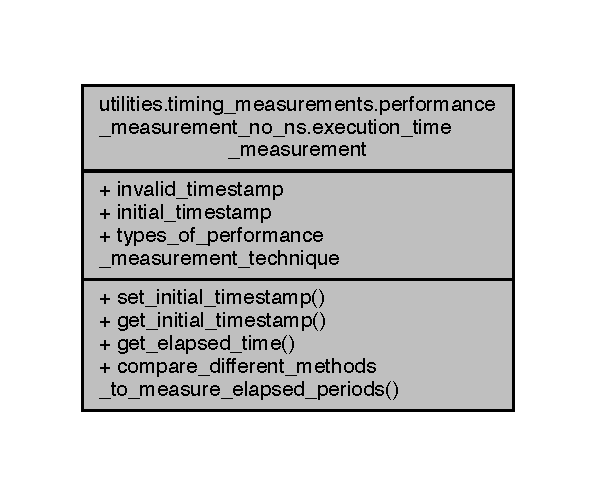
\includegraphics[width=286pt]{d1/d53/classutilities_1_1timing__measurements_1_1performance__measurement__no__ns_1_1execution__time__measurement__coll__graph}
\end{center}
\end{figure}
\subsection*{Static Public Member Functions}
\begin{DoxyCompactItemize}
\item 
def \hyperlink{classutilities_1_1timing__measurements_1_1performance__measurement__no__ns_1_1execution__time__measurement_ac1a396608592993d871613a73d20b088}{set\+\_\+initial\+\_\+timestamp}
\begin{DoxyCompactList}\small\item\em Method to set the initial timestamp. \end{DoxyCompactList}\item 
def \hyperlink{classutilities_1_1timing__measurements_1_1performance__measurement__no__ns_1_1execution__time__measurement_af12752f53bfd297b66b504170b9e3655}{get\+\_\+initial\+\_\+timestamp} ()
\begin{DoxyCompactList}\small\item\em Method to get the initial timestamp. \end{DoxyCompactList}\item 
def \hyperlink{classutilities_1_1timing__measurements_1_1performance__measurement__no__ns_1_1execution__time__measurement_a465918aa8dcf663887149cbf9a7306b9}{get\+\_\+elapsed\+\_\+time}
\begin{DoxyCompactList}\small\item\em Method to determine the elapsed time from the initial timestamp. \end{DoxyCompactList}\item 
def \hyperlink{classutilities_1_1timing__measurements_1_1performance__measurement__no__ns_1_1execution__time__measurement_a75eea39203f4d9b779977f9203f6d745}{compare\+\_\+different\+\_\+methods\+\_\+to\+\_\+measure\+\_\+elapsed\+\_\+periods} ()
\begin{DoxyCompactList}\small\item\em Method to compare techniques for measuring elapsed periods. \end{DoxyCompactList}\end{DoxyCompactItemize}
\subsection*{Static Public Attributes}
\begin{DoxyCompactItemize}
\item 
int \hyperlink{classutilities_1_1timing__measurements_1_1performance__measurement__no__ns_1_1execution__time__measurement_ac0b6b9477824b6d0b0e1348864d55566}{invalid\+\_\+timestamp} = -\/123456789012345678901234567890
\item 
\hyperlink{classutilities_1_1timing__measurements_1_1performance__measurement__no__ns_1_1execution__time__measurement_a75ac358ee6e04eba517fd6dd429c99a1}{initial\+\_\+timestamp} = \hyperlink{classutilities_1_1timing__measurements_1_1performance__measurement__no__ns_1_1execution__time__measurement_ac0b6b9477824b6d0b0e1348864d55566}{invalid\+\_\+timestamp}
\item 
tuple \hyperlink{classutilities_1_1timing__measurements_1_1performance__measurement__no__ns_1_1execution__time__measurement_aa73046ac445a5731739e52ae5034c4a1}{types\+\_\+of\+\_\+performance\+\_\+measurement\+\_\+technique} = (\char`\"{}perf\+\_\+counter\char`\"{},\char`\"{}process\+\_\+time\char`\"{},\char`\"{}time\char`\"{},\char`\"{}monotonic\char`\"{})
\end{DoxyCompactItemize}


\subsection{Detailed Description}


Definition at line \hyperlink{performance__measurement__no__ns_8py_source_l00115}{115} of file \hyperlink{performance__measurement__no__ns_8py_source}{performance\+\_\+measurement\+\_\+no\+\_\+ns.\+py}.



\subsection{Member Function Documentation}
\hypertarget{classutilities_1_1timing__measurements_1_1performance__measurement__no__ns_1_1execution__time__measurement_a75eea39203f4d9b779977f9203f6d745}{}\index{utilities\+::timing\+\_\+measurements\+::performance\+\_\+measurement\+\_\+no\+\_\+ns\+::execution\+\_\+time\+\_\+measurement@{utilities\+::timing\+\_\+measurements\+::performance\+\_\+measurement\+\_\+no\+\_\+ns\+::execution\+\_\+time\+\_\+measurement}!compare\+\_\+different\+\_\+methods\+\_\+to\+\_\+measure\+\_\+elapsed\+\_\+periods@{compare\+\_\+different\+\_\+methods\+\_\+to\+\_\+measure\+\_\+elapsed\+\_\+periods}}
\index{compare\+\_\+different\+\_\+methods\+\_\+to\+\_\+measure\+\_\+elapsed\+\_\+periods@{compare\+\_\+different\+\_\+methods\+\_\+to\+\_\+measure\+\_\+elapsed\+\_\+periods}!utilities\+::timing\+\_\+measurements\+::performance\+\_\+measurement\+\_\+no\+\_\+ns\+::execution\+\_\+time\+\_\+measurement@{utilities\+::timing\+\_\+measurements\+::performance\+\_\+measurement\+\_\+no\+\_\+ns\+::execution\+\_\+time\+\_\+measurement}}
\subsubsection[{compare\+\_\+different\+\_\+methods\+\_\+to\+\_\+measure\+\_\+elapsed\+\_\+periods()}]{\setlength{\rightskip}{0pt plus 5cm}def utilities.\+timing\+\_\+measurements.\+performance\+\_\+measurement\+\_\+no\+\_\+ns.\+execution\+\_\+time\+\_\+measurement.\+compare\+\_\+different\+\_\+methods\+\_\+to\+\_\+measure\+\_\+elapsed\+\_\+periods (
\begin{DoxyParamCaption}
{}
\end{DoxyParamCaption}
)\hspace{0.3cm}{\ttfamily [static]}}\label{classutilities_1_1timing__measurements_1_1performance__measurement__no__ns_1_1execution__time__measurement_a75eea39203f4d9b779977f9203f6d745}


Method to compare techniques for measuring elapsed periods. 

It calculates the factorial of each number in a list, and uses each of the following methods of performance measurement to measure the elapsed periods.
\begin{DoxyItemize}
\item perf\+\_\+counter, perf\+\_\+counter()\+: pc\+\_\+timestamp()
\item process\+\_\+time, process\+\_\+time()\+: pt\+\_\+timestamp()
\item time, time.\+time()\+: time()
\item monotonic, monotonic()\+: pm\+\_\+monotonic() \begin{DoxyReturn}{Returns}
-\/ Nothing. O(n!) method, where n is the largest number in the aforementioned list, since we are measuring the performance of calculating factorials. \begin{DoxyVerb}    Create a file to store experimental data of measuring
the performance of recursive and iterative methods.
\end{DoxyVerb}
 
\end{DoxyReturn}

\end{DoxyItemize}

Definition at line \hyperlink{performance__measurement__no__ns_8py_source_l00219}{219} of file \hyperlink{performance__measurement__no__ns_8py_source}{performance\+\_\+measurement\+\_\+no\+\_\+ns.\+py}.


\begin{DoxyCode}
\hypertarget{classutilities_1_1timing__measurements_1_1performance__measurement__no__ns_1_1execution__time__measurement_l00219}{}\hyperlink{classutilities_1_1timing__measurements_1_1performance__measurement__no__ns_1_1execution__time__measurement_a75eea39203f4d9b779977f9203f6d745}{00219}     \textcolor{keyword}{def }\hyperlink{classutilities_1_1timing__measurements_1_1performance__measurement__no__ns_1_1execution__time__measurement_a75eea39203f4d9b779977f9203f6d745}{compare\_different\_methods\_to\_measure\_elapsed\_periods}
      ():
00220         \textcolor{stringliteral}{"""}
00221 \textcolor{stringliteral}{            Create a file to store experimental data of measuring}
00222 \textcolor{stringliteral}{                the performance of recursive and iterative methods.}
00223 \textcolor{stringliteral}{        """}
00224         with open(\textcolor{stringliteral}{"compare\_different\_methods\_to\_measure\_elapsed\_periods.csv"},\textcolor{stringliteral}{"a+"}) \textcolor{keyword}{as} op\_f\_obj:
00225             \textcolor{keywordflow}{for} perf\_measurement\_technique \textcolor{keywordflow}{in} 
      execution\_time\_measurement.types\_of\_performance\_measurement\_technique:
00226                 print(\textcolor{stringliteral}{"The technique used is:"},perf\_measurement\_technique,\textcolor{stringliteral}{"="})
00227                 \textcolor{stringliteral}{"""}
00228 \textcolor{stringliteral}{                    Set the initial timestamp for calculating the}
00229 \textcolor{stringliteral}{                        factorial of numbers via recursion.}
00230 \textcolor{stringliteral}{                """}
00231                 execution\_time\_measurement.set\_initial\_timestamp(perf\_measurement\_technique)
00232                 print(\textcolor{stringliteral}{" Calculate the factorial using recursion."})
00233                 print(\textcolor{stringliteral}{" = current timestamp:"},execution\_time\_measurement.get\_initial\_timestamp(),\textcolor{stringliteral}{"="})
00234                 \textcolor{keywordflow}{for} x \textcolor{keywordflow}{in} range(0,20+1):
00235                     print(\textcolor{stringliteral}{"     factorial of"},x,\textcolor{stringliteral}{" is:"},calculate\_factorial.get\_factorial\_recursion(x),\textcolor{stringliteral}{"="})
00236                 \textcolor{stringliteral}{"""}
00237 \textcolor{stringliteral}{                    Get the elapsed time for calculating the factorial of}
00238 \textcolor{stringliteral}{                        numbers via recursion.}
00239 \textcolor{stringliteral}{                """}
00240                 elapsed\_time\_recursion = execution\_time\_measurement.get\_elapsed\_time(
      perf\_measurement\_technique)
00241                 print(\textcolor{stringliteral}{" = elapsed\_time\_recursion:"},elapsed\_time\_recursion,\textcolor{stringliteral}{"="})
00242                 \textcolor{stringliteral}{"""}
00243 \textcolor{stringliteral}{                    Set the initial timestamp for calculating the}
00244 \textcolor{stringliteral}{                        factorial of numbers via iteration.}
00245 \textcolor{stringliteral}{                """}
00246                 execution\_time\_measurement.set\_initial\_timestamp(perf\_measurement\_technique)
00247                 print(\textcolor{stringliteral}{" Calculate the factorial using iteration."})
00248                 print(\textcolor{stringliteral}{" = current timestamp:"},execution\_time\_measurement.get\_initial\_timestamp(),\textcolor{stringliteral}{"="})
00249                 \textcolor{keywordflow}{for} x \textcolor{keywordflow}{in} range(0,20+1):
00250                     print(\textcolor{stringliteral}{"     factorial of"},x,\textcolor{stringliteral}{" is:"},calculate\_factorial.get\_factorial\_iteration(x),\textcolor{stringliteral}{"="})
00251                 \textcolor{stringliteral}{"""}
00252 \textcolor{stringliteral}{                    Get the elapsed time for calculating the factorial of}
00253 \textcolor{stringliteral}{                        numbers via iteration.}
00254 \textcolor{stringliteral}{                """}
00255                 elapsed\_time\_iteration = execution\_time\_measurement.get\_elapsed\_time(
      perf\_measurement\_technique)
00256                 print(\textcolor{stringliteral}{" = elapsed\_time\_iteration:"},elapsed\_time\_iteration,\textcolor{stringliteral}{"="})
00257                 \textcolor{stringliteral}{"""}
00258 \textcolor{stringliteral}{                    The timeit.timeit() method can result in negative elapsed time.}
00259 \textcolor{stringliteral}{                """}
00260                 text = perf\_measurement\_technique + \textcolor{stringliteral}{","} + str(elapsed\_time\_recursion) + \textcolor{stringliteral}{","} + str(
      elapsed\_time\_iteration) + \textcolor{stringliteral}{"\(\backslash\)n"}
00261                 op\_f\_obj.write(text)
00262                 \textcolor{comment}{#op\_f\_obj.write("\(\backslash\)n")}
00263 
00264 
\end{DoxyCode}
\hypertarget{classutilities_1_1timing__measurements_1_1performance__measurement__no__ns_1_1execution__time__measurement_a465918aa8dcf663887149cbf9a7306b9}{}\index{utilities\+::timing\+\_\+measurements\+::performance\+\_\+measurement\+\_\+no\+\_\+ns\+::execution\+\_\+time\+\_\+measurement@{utilities\+::timing\+\_\+measurements\+::performance\+\_\+measurement\+\_\+no\+\_\+ns\+::execution\+\_\+time\+\_\+measurement}!get\+\_\+elapsed\+\_\+time@{get\+\_\+elapsed\+\_\+time}}
\index{get\+\_\+elapsed\+\_\+time@{get\+\_\+elapsed\+\_\+time}!utilities\+::timing\+\_\+measurements\+::performance\+\_\+measurement\+\_\+no\+\_\+ns\+::execution\+\_\+time\+\_\+measurement@{utilities\+::timing\+\_\+measurements\+::performance\+\_\+measurement\+\_\+no\+\_\+ns\+::execution\+\_\+time\+\_\+measurement}}
\subsubsection[{get\+\_\+elapsed\+\_\+time}]{\setlength{\rightskip}{0pt plus 5cm}def utilities.\+timing\+\_\+measurements.\+performance\+\_\+measurement\+\_\+no\+\_\+ns.\+execution\+\_\+time\+\_\+measurement.\+get\+\_\+elapsed\+\_\+time (
\begin{DoxyParamCaption}
\item[{}]{type\+\_\+timestamp = {\ttfamily \char`\"{}monotonic\char`\"{}}}
\end{DoxyParamCaption}
)\hspace{0.3cm}{\ttfamily [static]}}\label{classutilities_1_1timing__measurements_1_1performance__measurement__no__ns_1_1execution__time__measurement_a465918aa8dcf663887149cbf9a7306b9}


Method to determine the elapsed time from the initial timestamp. 


\begin{DoxyParams}{Parameters}
{\em type\+\_\+timestamp} & -\/ Indicates if either of the following methods of performance measurement is preferred.
\begin{DoxyItemize}
\item perf\+\_\+counter, perf\+\_\+counter()\+: pc\+\_\+timestamp()
\item process\+\_\+time, process\+\_\+time()\+: pt\+\_\+timestamp()
\item time, time.\+time\+\_\+ns()\+: time\+\_\+ns()
\item monotonic, monotonic()\+: pm\+\_\+monotonic() 
\end{DoxyItemize}\\
\hline
\end{DoxyParams}
\begin{DoxyReturn}{Returns}
the elapsed time from the initial timestamp. O(1) method. \begin{DoxyVerb}    Is the option for one of the following methods to measure
time?
* perf_counter, perf_counter(): pc_timestamp()
* process_time, process_time(): pt_timestamp()
* time, time.time_ns(): time_ns()
* monotonic, monotonic(): pm_monotonic()
\end{DoxyVerb}
 
\end{DoxyReturn}


Definition at line \hyperlink{performance__measurement__no__ns_8py_source_l00180}{180} of file \hyperlink{performance__measurement__no__ns_8py_source}{performance\+\_\+measurement\+\_\+no\+\_\+ns.\+py}.


\begin{DoxyCode}
\hypertarget{classutilities_1_1timing__measurements_1_1performance__measurement__no__ns_1_1execution__time__measurement_l00180}{}\hyperlink{classutilities_1_1timing__measurements_1_1performance__measurement__no__ns_1_1execution__time__measurement_a465918aa8dcf663887149cbf9a7306b9}{00180}     \textcolor{keyword}{def }\hyperlink{classutilities_1_1timing__measurements_1_1performance__measurement__no__ns_1_1execution__time__measurement_a465918aa8dcf663887149cbf9a7306b9}{get\_elapsed\_time}(type\_timestamp="monotonic"):
00181         \textcolor{stringliteral}{"""}
00182 \textcolor{stringliteral}{            Is the option for one of the following methods to measure}
00183 \textcolor{stringliteral}{                time?}
00184 \textcolor{stringliteral}{                * perf\_counter, perf\_counter(): pc\_timestamp()}
00185 \textcolor{stringliteral}{                * process\_time, process\_time(): pt\_timestamp()}
00186 \textcolor{stringliteral}{                * time, time.time\_ns(): time\_ns()}
00187 \textcolor{stringliteral}{                * monotonic, monotonic(): pm\_monotonic()}
00188 \textcolor{stringliteral}{        """}
00189         \textcolor{keywordflow}{if} (\textcolor{stringliteral}{"perf\_counter"} == type\_timestamp):
00190             \textcolor{comment}{# Yes. Use perf\_counter() to measure performance/time.}
00191             current\_timestamp = pc\_timestamp()
00192         \textcolor{keywordflow}{elif} (\textcolor{stringliteral}{"process\_time"} == type\_timestamp):
00193             \textcolor{comment}{# Yes. Use process\_time() to measure performance/time.}
00194             current\_timestamp = pt\_timestamp()
00195         \textcolor{keywordflow}{elif} (\textcolor{stringliteral}{"time"} == type\_timestamp):
00196             \textcolor{comment}{# Yes. Use time.time() to measure performance/time.}
00197             current\_timestamp = time.time()
00198         \textcolor{keywordflow}{else}:
00199             \textcolor{stringliteral}{"""}
00200 \textcolor{stringliteral}{                The default option is: "monotonic".}
00201 \textcolor{stringliteral}{                Use monotonic() to measure performance/time.}
00202 \textcolor{stringliteral}{            """}
00203             current\_timestamp = pm\_monotonic()
00204         \textcolor{keywordflow}{return} (current\_timestamp - execution\_time\_measurement.get\_initial\_timestamp())
\end{DoxyCode}
\hypertarget{classutilities_1_1timing__measurements_1_1performance__measurement__no__ns_1_1execution__time__measurement_af12752f53bfd297b66b504170b9e3655}{}\index{utilities\+::timing\+\_\+measurements\+::performance\+\_\+measurement\+\_\+no\+\_\+ns\+::execution\+\_\+time\+\_\+measurement@{utilities\+::timing\+\_\+measurements\+::performance\+\_\+measurement\+\_\+no\+\_\+ns\+::execution\+\_\+time\+\_\+measurement}!get\+\_\+initial\+\_\+timestamp@{get\+\_\+initial\+\_\+timestamp}}
\index{get\+\_\+initial\+\_\+timestamp@{get\+\_\+initial\+\_\+timestamp}!utilities\+::timing\+\_\+measurements\+::performance\+\_\+measurement\+\_\+no\+\_\+ns\+::execution\+\_\+time\+\_\+measurement@{utilities\+::timing\+\_\+measurements\+::performance\+\_\+measurement\+\_\+no\+\_\+ns\+::execution\+\_\+time\+\_\+measurement}}
\subsubsection[{get\+\_\+initial\+\_\+timestamp()}]{\setlength{\rightskip}{0pt plus 5cm}def utilities.\+timing\+\_\+measurements.\+performance\+\_\+measurement\+\_\+no\+\_\+ns.\+execution\+\_\+time\+\_\+measurement.\+get\+\_\+initial\+\_\+timestamp (
\begin{DoxyParamCaption}
{}
\end{DoxyParamCaption}
)\hspace{0.3cm}{\ttfamily [static]}}\label{classutilities_1_1timing__measurements_1_1performance__measurement__no__ns_1_1execution__time__measurement_af12752f53bfd297b66b504170b9e3655}


Method to get the initial timestamp. 

\begin{DoxyReturn}{Returns}
the initial timestamp. O(1) method. 
\end{DoxyReturn}


Definition at line \hyperlink{performance__measurement__no__ns_8py_source_l00166}{166} of file \hyperlink{performance__measurement__no__ns_8py_source}{performance\+\_\+measurement\+\_\+no\+\_\+ns.\+py}.


\begin{DoxyCode}
\hypertarget{classutilities_1_1timing__measurements_1_1performance__measurement__no__ns_1_1execution__time__measurement_l00166}{}\hyperlink{classutilities_1_1timing__measurements_1_1performance__measurement__no__ns_1_1execution__time__measurement_af12752f53bfd297b66b504170b9e3655}{00166}     \textcolor{keyword}{def }\hyperlink{classutilities_1_1timing__measurements_1_1performance__measurement__no__ns_1_1execution__time__measurement_af12752f53bfd297b66b504170b9e3655}{get\_initial\_timestamp}():
00167         \textcolor{keywordflow}{return} execution\_time\_measurement.initial\_timestamp
\end{DoxyCode}
\hypertarget{classutilities_1_1timing__measurements_1_1performance__measurement__no__ns_1_1execution__time__measurement_ac1a396608592993d871613a73d20b088}{}\index{utilities\+::timing\+\_\+measurements\+::performance\+\_\+measurement\+\_\+no\+\_\+ns\+::execution\+\_\+time\+\_\+measurement@{utilities\+::timing\+\_\+measurements\+::performance\+\_\+measurement\+\_\+no\+\_\+ns\+::execution\+\_\+time\+\_\+measurement}!set\+\_\+initial\+\_\+timestamp@{set\+\_\+initial\+\_\+timestamp}}
\index{set\+\_\+initial\+\_\+timestamp@{set\+\_\+initial\+\_\+timestamp}!utilities\+::timing\+\_\+measurements\+::performance\+\_\+measurement\+\_\+no\+\_\+ns\+::execution\+\_\+time\+\_\+measurement@{utilities\+::timing\+\_\+measurements\+::performance\+\_\+measurement\+\_\+no\+\_\+ns\+::execution\+\_\+time\+\_\+measurement}}
\subsubsection[{set\+\_\+initial\+\_\+timestamp}]{\setlength{\rightskip}{0pt plus 5cm}def utilities.\+timing\+\_\+measurements.\+performance\+\_\+measurement\+\_\+no\+\_\+ns.\+execution\+\_\+time\+\_\+measurement.\+set\+\_\+initial\+\_\+timestamp (
\begin{DoxyParamCaption}
\item[{}]{type\+\_\+timestamp = {\ttfamily \char`\"{}monotonic\char`\"{}}}
\end{DoxyParamCaption}
)\hspace{0.3cm}{\ttfamily [static]}}\label{classutilities_1_1timing__measurements_1_1performance__measurement__no__ns_1_1execution__time__measurement_ac1a396608592993d871613a73d20b088}


Method to set the initial timestamp. 

Use techniques for measuring performance (i.\+e., user execution time) and timestamps.

\begin{DoxyVerb}@param type_timestamp - Indicates if either of the following
            methods of performance measurement is preferred.
            * perf_counter, perf_counter(): pc_timestamp()
            * process_time, process_time(): pt_timestamp()
            * time, time.time(): time()
            * monotonic, monotonic(): pm_monotonic()
@return - Nothing.
O(1) method. \end{DoxyVerb}
 \begin{DoxyVerb}    Is the option for one of the following methods to measure
time?
* perf_counter, perf_counter(): pc_timestamp()
* process_time, process_time(): pt_timestamp()
* time, time.time(): time.time()
* monotonic, monotonic(): pm_monotonic()
\end{DoxyVerb}
 

Definition at line \hyperlink{performance__measurement__no__ns_8py_source_l00140}{140} of file \hyperlink{performance__measurement__no__ns_8py_source}{performance\+\_\+measurement\+\_\+no\+\_\+ns.\+py}.


\begin{DoxyCode}
\hypertarget{classutilities_1_1timing__measurements_1_1performance__measurement__no__ns_1_1execution__time__measurement_l00140}{}\hyperlink{classutilities_1_1timing__measurements_1_1performance__measurement__no__ns_1_1execution__time__measurement_ac1a396608592993d871613a73d20b088}{00140}     \textcolor{keyword}{def }\hyperlink{classutilities_1_1timing__measurements_1_1performance__measurement__no__ns_1_1execution__time__measurement_ac1a396608592993d871613a73d20b088}{set\_initial\_timestamp}(type\_timestamp="monotonic"):
00141         \textcolor{stringliteral}{"""}
00142 \textcolor{stringliteral}{            Is the option for one of the following methods to measure}
00143 \textcolor{stringliteral}{                time?}
00144 \textcolor{stringliteral}{                * perf\_counter, perf\_counter(): pc\_timestamp()}
00145 \textcolor{stringliteral}{                * process\_time, process\_time(): pt\_timestamp()}
00146 \textcolor{stringliteral}{                * time, time.time(): time.time()}
00147 \textcolor{stringliteral}{                * monotonic, monotonic(): pm\_monotonic()}
00148 \textcolor{stringliteral}{        """}
00149         \textcolor{keywordflow}{if} (\textcolor{stringliteral}{"perf\_counter"} == type\_timestamp):
00150             \textcolor{comment}{# Yes. Use perf\_counter() to measure performance/time.}
00151             execution\_time\_measurement.initial\_timestamp = pc\_timestamp()
00152         \textcolor{keywordflow}{elif} (\textcolor{stringliteral}{"process\_time"} == type\_timestamp):
00153             \textcolor{comment}{# Yes. Use process\_time() to measure performance/time.}
00154             execution\_time\_measurement.initial\_timestamp = pt\_timestamp()
00155         \textcolor{keywordflow}{elif} (\textcolor{stringliteral}{"time"} == type\_timestamp):
00156             \textcolor{comment}{# Yes. Use time() to measure performance/time.}
00157             execution\_time\_measurement.initial\_timestamp = time.time()
00158         \textcolor{keywordflow}{else}:
00159             \textcolor{comment}{# The default option is: "monotonic()"}
00160             execution\_time\_measurement.initial\_timestamp = pm\_monotonic()
\end{DoxyCode}


\subsection{Member Data Documentation}
\hypertarget{classutilities_1_1timing__measurements_1_1performance__measurement__no__ns_1_1execution__time__measurement_a75ac358ee6e04eba517fd6dd429c99a1}{}\index{utilities\+::timing\+\_\+measurements\+::performance\+\_\+measurement\+\_\+no\+\_\+ns\+::execution\+\_\+time\+\_\+measurement@{utilities\+::timing\+\_\+measurements\+::performance\+\_\+measurement\+\_\+no\+\_\+ns\+::execution\+\_\+time\+\_\+measurement}!initial\+\_\+timestamp@{initial\+\_\+timestamp}}
\index{initial\+\_\+timestamp@{initial\+\_\+timestamp}!utilities\+::timing\+\_\+measurements\+::performance\+\_\+measurement\+\_\+no\+\_\+ns\+::execution\+\_\+time\+\_\+measurement@{utilities\+::timing\+\_\+measurements\+::performance\+\_\+measurement\+\_\+no\+\_\+ns\+::execution\+\_\+time\+\_\+measurement}}
\subsubsection[{initial\+\_\+timestamp}]{\setlength{\rightskip}{0pt plus 5cm}utilities.\+timing\+\_\+measurements.\+performance\+\_\+measurement\+\_\+no\+\_\+ns.\+execution\+\_\+time\+\_\+measurement.\+initial\+\_\+timestamp = {\bf invalid\+\_\+timestamp}\hspace{0.3cm}{\ttfamily [static]}}\label{classutilities_1_1timing__measurements_1_1performance__measurement__no__ns_1_1execution__time__measurement_a75ac358ee6e04eba517fd6dd429c99a1}


Definition at line \hyperlink{performance__measurement__no__ns_8py_source_l00119}{119} of file \hyperlink{performance__measurement__no__ns_8py_source}{performance\+\_\+measurement\+\_\+no\+\_\+ns.\+py}.

\hypertarget{classutilities_1_1timing__measurements_1_1performance__measurement__no__ns_1_1execution__time__measurement_ac0b6b9477824b6d0b0e1348864d55566}{}\index{utilities\+::timing\+\_\+measurements\+::performance\+\_\+measurement\+\_\+no\+\_\+ns\+::execution\+\_\+time\+\_\+measurement@{utilities\+::timing\+\_\+measurements\+::performance\+\_\+measurement\+\_\+no\+\_\+ns\+::execution\+\_\+time\+\_\+measurement}!invalid\+\_\+timestamp@{invalid\+\_\+timestamp}}
\index{invalid\+\_\+timestamp@{invalid\+\_\+timestamp}!utilities\+::timing\+\_\+measurements\+::performance\+\_\+measurement\+\_\+no\+\_\+ns\+::execution\+\_\+time\+\_\+measurement@{utilities\+::timing\+\_\+measurements\+::performance\+\_\+measurement\+\_\+no\+\_\+ns\+::execution\+\_\+time\+\_\+measurement}}
\subsubsection[{invalid\+\_\+timestamp}]{\setlength{\rightskip}{0pt plus 5cm}int utilities.\+timing\+\_\+measurements.\+performance\+\_\+measurement\+\_\+no\+\_\+ns.\+execution\+\_\+time\+\_\+measurement.\+invalid\+\_\+timestamp = -\/123456789012345678901234567890\hspace{0.3cm}{\ttfamily [static]}}\label{classutilities_1_1timing__measurements_1_1performance__measurement__no__ns_1_1execution__time__measurement_ac0b6b9477824b6d0b0e1348864d55566}


Definition at line \hyperlink{performance__measurement__no__ns_8py_source_l00117}{117} of file \hyperlink{performance__measurement__no__ns_8py_source}{performance\+\_\+measurement\+\_\+no\+\_\+ns.\+py}.

\hypertarget{classutilities_1_1timing__measurements_1_1performance__measurement__no__ns_1_1execution__time__measurement_aa73046ac445a5731739e52ae5034c4a1}{}\index{utilities\+::timing\+\_\+measurements\+::performance\+\_\+measurement\+\_\+no\+\_\+ns\+::execution\+\_\+time\+\_\+measurement@{utilities\+::timing\+\_\+measurements\+::performance\+\_\+measurement\+\_\+no\+\_\+ns\+::execution\+\_\+time\+\_\+measurement}!types\+\_\+of\+\_\+performance\+\_\+measurement\+\_\+technique@{types\+\_\+of\+\_\+performance\+\_\+measurement\+\_\+technique}}
\index{types\+\_\+of\+\_\+performance\+\_\+measurement\+\_\+technique@{types\+\_\+of\+\_\+performance\+\_\+measurement\+\_\+technique}!utilities\+::timing\+\_\+measurements\+::performance\+\_\+measurement\+\_\+no\+\_\+ns\+::execution\+\_\+time\+\_\+measurement@{utilities\+::timing\+\_\+measurements\+::performance\+\_\+measurement\+\_\+no\+\_\+ns\+::execution\+\_\+time\+\_\+measurement}}
\subsubsection[{types\+\_\+of\+\_\+performance\+\_\+measurement\+\_\+technique}]{\setlength{\rightskip}{0pt plus 5cm}tuple utilities.\+timing\+\_\+measurements.\+performance\+\_\+measurement\+\_\+no\+\_\+ns.\+execution\+\_\+time\+\_\+measurement.\+types\+\_\+of\+\_\+performance\+\_\+measurement\+\_\+technique = (\char`\"{}perf\+\_\+counter\char`\"{},\char`\"{}process\+\_\+time\char`\"{},\char`\"{}time\char`\"{},\char`\"{}monotonic\char`\"{})\hspace{0.3cm}{\ttfamily [static]}}\label{classutilities_1_1timing__measurements_1_1performance__measurement__no__ns_1_1execution__time__measurement_aa73046ac445a5731739e52ae5034c4a1}


Definition at line \hyperlink{performance__measurement__no__ns_8py_source_l00122}{122} of file \hyperlink{performance__measurement__no__ns_8py_source}{performance\+\_\+measurement\+\_\+no\+\_\+ns.\+py}.



The documentation for this class was generated from the following file\+:\begin{DoxyCompactItemize}
\item 
utilities/timing\+\_\+measurements/\hyperlink{performance__measurement__no__ns_8py}{performance\+\_\+measurement\+\_\+no\+\_\+ns.\+py}\end{DoxyCompactItemize}

\hypertarget{classutilities_1_1timing__measurements_1_1performance__measurement_1_1execution__time__measurement}{}\section{utilities.\+timing\+\_\+measurements.\+performance\+\_\+measurement.\+execution\+\_\+time\+\_\+measurement Class Reference}
\label{classutilities_1_1timing__measurements_1_1performance__measurement_1_1execution__time__measurement}\index{utilities.\+timing\+\_\+measurements.\+performance\+\_\+measurement.\+execution\+\_\+time\+\_\+measurement@{utilities.\+timing\+\_\+measurements.\+performance\+\_\+measurement.\+execution\+\_\+time\+\_\+measurement}}


Collaboration diagram for utilities.\+timing\+\_\+measurements.\+performance\+\_\+measurement.\+execution\+\_\+time\+\_\+measurement\+:
\nopagebreak
\begin{figure}[H]
\begin{center}
\leavevmode
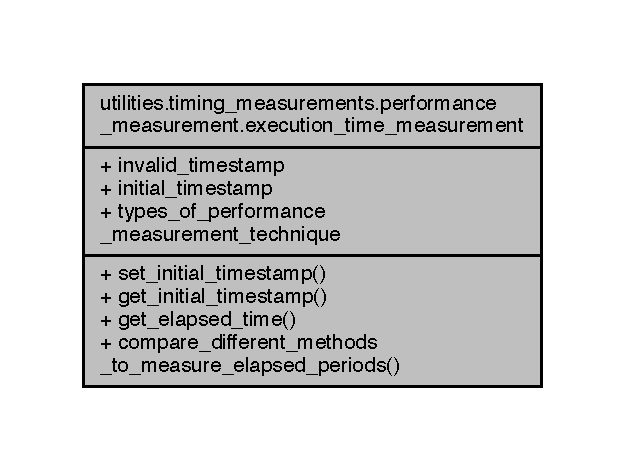
\includegraphics[width=300pt]{db/db8/classutilities_1_1timing__measurements_1_1performance__measurement_1_1execution__time__measurement__coll__graph}
\end{center}
\end{figure}
\subsection*{Static Public Member Functions}
\begin{DoxyCompactItemize}
\item 
def \hyperlink{classutilities_1_1timing__measurements_1_1performance__measurement_1_1execution__time__measurement_aa82fdf41b58ed820066c6f74450a2e66}{set\+\_\+initial\+\_\+timestamp}
\begin{DoxyCompactList}\small\item\em Method to set the initial timestamp. \end{DoxyCompactList}\item 
def \hyperlink{classutilities_1_1timing__measurements_1_1performance__measurement_1_1execution__time__measurement_a8737db6c2fdb833d0d30d80c70ffebb0}{get\+\_\+initial\+\_\+timestamp} ()
\begin{DoxyCompactList}\small\item\em Method to get the initial timestamp. \end{DoxyCompactList}\item 
def \hyperlink{classutilities_1_1timing__measurements_1_1performance__measurement_1_1execution__time__measurement_a02b1d7ffce2b4c702a82a03803322e65}{get\+\_\+elapsed\+\_\+time}
\begin{DoxyCompactList}\small\item\em Method to determine the elapsed time from the initial timestamp. \end{DoxyCompactList}\item 
def \hyperlink{classutilities_1_1timing__measurements_1_1performance__measurement_1_1execution__time__measurement_a9b05f1fd5acd56880daa42266dbf8284}{compare\+\_\+different\+\_\+methods\+\_\+to\+\_\+measure\+\_\+elapsed\+\_\+periods} ()
\begin{DoxyCompactList}\small\item\em Method to compare techniques for measuring elapsed periods. \end{DoxyCompactList}\end{DoxyCompactItemize}
\subsection*{Static Public Attributes}
\begin{DoxyCompactItemize}
\item 
int \hyperlink{classutilities_1_1timing__measurements_1_1performance__measurement_1_1execution__time__measurement_a3d083e8440c081f0a39ecea850d3cb67}{invalid\+\_\+timestamp} = -\/123456789012345678901234567890
\item 
\hyperlink{classutilities_1_1timing__measurements_1_1performance__measurement_1_1execution__time__measurement_ac60d39fb6affbaa3d6eb2792c41ee7ff}{initial\+\_\+timestamp} = \hyperlink{classutilities_1_1timing__measurements_1_1performance__measurement_1_1execution__time__measurement_a3d083e8440c081f0a39ecea850d3cb67}{invalid\+\_\+timestamp}
\item 
tuple \hyperlink{classutilities_1_1timing__measurements_1_1performance__measurement_1_1execution__time__measurement_a80ff3ce9b405f5d8c2e63294348ca6dc}{types\+\_\+of\+\_\+performance\+\_\+measurement\+\_\+technique} = (\char`\"{}perf\+\_\+counter\char`\"{},\char`\"{}perf\+\_\+counter\+\_\+ns\char`\"{},\char`\"{}process\+\_\+time\char`\"{},\char`\"{}process\+\_\+time\+\_\+ns\char`\"{},\char`\"{}time\char`\"{},\char`\"{}time\+\_\+ns\char`\"{},\char`\"{}monotonic\char`\"{},\char`\"{}monotonic\+\_\+ns\char`\"{})
\end{DoxyCompactItemize}


\subsection{Detailed Description}


Definition at line \hyperlink{performance__measurement_8py_source_l00115}{115} of file \hyperlink{performance__measurement_8py_source}{performance\+\_\+measurement.\+py}.



\subsection{Member Function Documentation}
\hypertarget{classutilities_1_1timing__measurements_1_1performance__measurement_1_1execution__time__measurement_a9b05f1fd5acd56880daa42266dbf8284}{}\index{utilities\+::timing\+\_\+measurements\+::performance\+\_\+measurement\+::execution\+\_\+time\+\_\+measurement@{utilities\+::timing\+\_\+measurements\+::performance\+\_\+measurement\+::execution\+\_\+time\+\_\+measurement}!compare\+\_\+different\+\_\+methods\+\_\+to\+\_\+measure\+\_\+elapsed\+\_\+periods@{compare\+\_\+different\+\_\+methods\+\_\+to\+\_\+measure\+\_\+elapsed\+\_\+periods}}
\index{compare\+\_\+different\+\_\+methods\+\_\+to\+\_\+measure\+\_\+elapsed\+\_\+periods@{compare\+\_\+different\+\_\+methods\+\_\+to\+\_\+measure\+\_\+elapsed\+\_\+periods}!utilities\+::timing\+\_\+measurements\+::performance\+\_\+measurement\+::execution\+\_\+time\+\_\+measurement@{utilities\+::timing\+\_\+measurements\+::performance\+\_\+measurement\+::execution\+\_\+time\+\_\+measurement}}
\subsubsection[{compare\+\_\+different\+\_\+methods\+\_\+to\+\_\+measure\+\_\+elapsed\+\_\+periods()}]{\setlength{\rightskip}{0pt plus 5cm}def utilities.\+timing\+\_\+measurements.\+performance\+\_\+measurement.\+execution\+\_\+time\+\_\+measurement.\+compare\+\_\+different\+\_\+methods\+\_\+to\+\_\+measure\+\_\+elapsed\+\_\+periods (
\begin{DoxyParamCaption}
{}
\end{DoxyParamCaption}
)\hspace{0.3cm}{\ttfamily [static]}}\label{classutilities_1_1timing__measurements_1_1performance__measurement_1_1execution__time__measurement_a9b05f1fd5acd56880daa42266dbf8284}


Method to compare techniques for measuring elapsed periods. 

It calculates the factorial of each number in a list, and uses each of the following methods of performance measurement to measure the elapsed periods.
\begin{DoxyItemize}
\item perf\+\_\+counter, perf\+\_\+counter()\+: pc\+\_\+timestamp()
\item perf\+\_\+counter\+\_\+ns, perf\+\_\+counter\+\_\+ns()\+: pc\+\_\+timestamp\+\_\+ns()
\item process\+\_\+time, process\+\_\+time()\+: pt\+\_\+timestamp()
\item process\+\_\+time\+\_\+ns, process\+\_\+time\+\_\+ns()\+: pt\+\_\+timestamp\+\_\+ns()
\item time, time.\+time()\+: time()
\item time\+\_\+ns, time.\+time\+\_\+ns()\+: time\+\_\+ns()
\item monotonic, monotonic()\+: pm\+\_\+monotonic()
\item monotonic\+\_\+ns, monotonic\+\_\+ns()\+: pm\+\_\+monotonic\+\_\+ns() \begin{DoxyReturn}{Returns}
-\/ Nothing. O(n!) method, where n is the largest number in the aforementioned list, since we are measuring the performance of calculating factorials. \begin{DoxyVerb}    Create a file to store experimental data of measuring
the performance of recursive and iterative methods.
\end{DoxyVerb}
 
\end{DoxyReturn}

\end{DoxyItemize}

Definition at line \hyperlink{performance__measurement_8py_source_l00262}{262} of file \hyperlink{performance__measurement_8py_source}{performance\+\_\+measurement.\+py}.


\begin{DoxyCode}
\hypertarget{classutilities_1_1timing__measurements_1_1performance__measurement_1_1execution__time__measurement_l00262}{}\hyperlink{classutilities_1_1timing__measurements_1_1performance__measurement_1_1execution__time__measurement_a9b05f1fd5acd56880daa42266dbf8284}{00262}     \textcolor{keyword}{def }\hyperlink{classutilities_1_1timing__measurements_1_1performance__measurement_1_1execution__time__measurement_a9b05f1fd5acd56880daa42266dbf8284}{compare\_different\_methods\_to\_measure\_elapsed\_periods}
      ():
00263         \textcolor{stringliteral}{"""}
00264 \textcolor{stringliteral}{            Create a file to store experimental data of measuring}
00265 \textcolor{stringliteral}{                the performance of recursive and iterative methods.}
00266 \textcolor{stringliteral}{        """}
00267         with open(\textcolor{stringliteral}{"compare\_different\_methods\_to\_measure\_elapsed\_periods.csv"},\textcolor{stringliteral}{"a+"}) \textcolor{keyword}{as} op\_f\_obj:
00268             \textcolor{keywordflow}{for} perf\_measurement\_technique \textcolor{keywordflow}{in} 
      execution\_time\_measurement.types\_of\_performance\_measurement\_technique:
00269                 print(\textcolor{stringliteral}{"The technique used is:"},perf\_measurement\_technique,\textcolor{stringliteral}{"="})
00270                 \textcolor{stringliteral}{"""}
00271 \textcolor{stringliteral}{                    Set the initial timestamp for calculating the}
00272 \textcolor{stringliteral}{                        factorial of numbers via recursion.}
00273 \textcolor{stringliteral}{                """}
00274                 execution\_time\_measurement.set\_initial\_timestamp(perf\_measurement\_technique)
00275                 print(\textcolor{stringliteral}{" Calculate the factorial using recursion."})
00276                 print(\textcolor{stringliteral}{" = current timestamp:"},execution\_time\_measurement.get\_initial\_timestamp(),\textcolor{stringliteral}{"="})
00277                 \textcolor{keywordflow}{for} x \textcolor{keywordflow}{in} range(0,20+1):
00278                     print(\textcolor{stringliteral}{"     factorial of"},x,\textcolor{stringliteral}{" is:"},calculate\_factorial.get\_factorial\_recursion(x),\textcolor{stringliteral}{"="})
00279                 \textcolor{stringliteral}{"""}
00280 \textcolor{stringliteral}{                    Get the elapsed time for calculating the factorial of}
00281 \textcolor{stringliteral}{                        numbers via recursion.}
00282 \textcolor{stringliteral}{                """}
00283                 elapsed\_time\_recursion = execution\_time\_measurement.get\_elapsed\_time(
      perf\_measurement\_technique)
00284                 print(\textcolor{stringliteral}{" = elapsed\_time\_recursion:"},elapsed\_time\_recursion,\textcolor{stringliteral}{"="})
00285                 \textcolor{stringliteral}{"""}
00286 \textcolor{stringliteral}{                    Set the initial timestamp for calculating the}
00287 \textcolor{stringliteral}{                        factorial of numbers via iteration.}
00288 \textcolor{stringliteral}{                """}
00289                 execution\_time\_measurement.set\_initial\_timestamp(perf\_measurement\_technique)
00290                 print(\textcolor{stringliteral}{" Calculate the factorial using iteration."})
00291                 print(\textcolor{stringliteral}{" = current timestamp:"},execution\_time\_measurement.get\_initial\_timestamp(),\textcolor{stringliteral}{"="})
00292                 \textcolor{keywordflow}{for} x \textcolor{keywordflow}{in} range(0,20+1):
00293                     print(\textcolor{stringliteral}{"     factorial of"},x,\textcolor{stringliteral}{" is:"},calculate\_factorial.get\_factorial\_iteration(x),\textcolor{stringliteral}{"="})
00294                 \textcolor{stringliteral}{"""}
00295 \textcolor{stringliteral}{                    Get the elapsed time for calculating the factorial of}
00296 \textcolor{stringliteral}{                        numbers via iteration.}
00297 \textcolor{stringliteral}{                """}
00298                 elapsed\_time\_iteration = execution\_time\_measurement.get\_elapsed\_time(
      perf\_measurement\_technique)
00299                 print(\textcolor{stringliteral}{" = elapsed\_time\_iteration:"},elapsed\_time\_iteration,\textcolor{stringliteral}{"="})
00300                 \textcolor{stringliteral}{"""}
00301 \textcolor{stringliteral}{                    The timeit.timeit() method can result in negative elapsed time.}
00302 \textcolor{stringliteral}{                """}
00303                 text = perf\_measurement\_technique + \textcolor{stringliteral}{","} + str(elapsed\_time\_recursion) + \textcolor{stringliteral}{","} + str(
      elapsed\_time\_iteration) + \textcolor{stringliteral}{"\(\backslash\)n"}
00304                 op\_f\_obj.write(text)
00305                 \textcolor{comment}{#op\_f\_obj.write("\(\backslash\)n")}
00306 
00307 
\end{DoxyCode}
\hypertarget{classutilities_1_1timing__measurements_1_1performance__measurement_1_1execution__time__measurement_a02b1d7ffce2b4c702a82a03803322e65}{}\index{utilities\+::timing\+\_\+measurements\+::performance\+\_\+measurement\+::execution\+\_\+time\+\_\+measurement@{utilities\+::timing\+\_\+measurements\+::performance\+\_\+measurement\+::execution\+\_\+time\+\_\+measurement}!get\+\_\+elapsed\+\_\+time@{get\+\_\+elapsed\+\_\+time}}
\index{get\+\_\+elapsed\+\_\+time@{get\+\_\+elapsed\+\_\+time}!utilities\+::timing\+\_\+measurements\+::performance\+\_\+measurement\+::execution\+\_\+time\+\_\+measurement@{utilities\+::timing\+\_\+measurements\+::performance\+\_\+measurement\+::execution\+\_\+time\+\_\+measurement}}
\subsubsection[{get\+\_\+elapsed\+\_\+time}]{\setlength{\rightskip}{0pt plus 5cm}def utilities.\+timing\+\_\+measurements.\+performance\+\_\+measurement.\+execution\+\_\+time\+\_\+measurement.\+get\+\_\+elapsed\+\_\+time (
\begin{DoxyParamCaption}
\item[{}]{type\+\_\+timestamp = {\ttfamily \char`\"{}monotonic\+\_\+ns\char`\"{}}}
\end{DoxyParamCaption}
)\hspace{0.3cm}{\ttfamily [static]}}\label{classutilities_1_1timing__measurements_1_1performance__measurement_1_1execution__time__measurement_a02b1d7ffce2b4c702a82a03803322e65}


Method to determine the elapsed time from the initial timestamp. 


\begin{DoxyParams}{Parameters}
{\em type\+\_\+timestamp} & -\/ Indicates if either of the following methods of performance measurement is preferred.
\begin{DoxyItemize}
\item perf\+\_\+counter, perf\+\_\+counter()\+: pc\+\_\+timestamp()
\item perf\+\_\+counter\+\_\+ns, perf\+\_\+counter\+\_\+ns()\+: pc\+\_\+timestamp\+\_\+ns()
\item process\+\_\+time, process\+\_\+time()\+: pt\+\_\+timestamp()
\item process\+\_\+time\+\_\+ns, process\+\_\+time\+\_\+ns()\+: pt\+\_\+timestamp\+\_\+ns()
\item time, time.\+time()\+: time()
\item time\+\_\+ns, time.\+time\+\_\+ns()\+: time\+\_\+ns()
\item monotonic, monotonic()\+: pm\+\_\+monotonic()
\item monotonic\+\_\+ns, monotonic\+\_\+ns()\+: pm\+\_\+monotonic\+\_\+ns() 
\end{DoxyItemize}\\
\hline
\end{DoxyParams}
\begin{DoxyReturn}{Returns}
the elapsed time from the initial timestamp. O(1) method. \begin{DoxyVerb}    Is the option for one of the following methods to measure
time?
* perf_counter, perf_counter(): pc_timestamp()
* perf_counter_ns, perf_counter_ns(): pc_timestamp_ns()
* process_time, process_time(): pt_timestamp()
* process_time_ns, process_time_ns(): pt_timestamp_ns()
* time, time.time(): time()
* time_ns, time.time_ns(): time_ns()
* monotonic, monotonic(): pm_monotonic()
* monotonic_ns, monotonic_ns(): pm_monotonic_ns()
\end{DoxyVerb}
 
\end{DoxyReturn}


Definition at line \hyperlink{performance__measurement_8py_source_l00203}{203} of file \hyperlink{performance__measurement_8py_source}{performance\+\_\+measurement.\+py}.


\begin{DoxyCode}
\hypertarget{classutilities_1_1timing__measurements_1_1performance__measurement_1_1execution__time__measurement_l00203}{}\hyperlink{classutilities_1_1timing__measurements_1_1performance__measurement_1_1execution__time__measurement_a02b1d7ffce2b4c702a82a03803322e65}{00203}     \textcolor{keyword}{def }\hyperlink{classutilities_1_1timing__measurements_1_1performance__measurement_1_1execution__time__measurement_a02b1d7ffce2b4c702a82a03803322e65}{get\_elapsed\_time}(type\_timestamp="monotonic\_ns"):
00204         \textcolor{stringliteral}{"""}
00205 \textcolor{stringliteral}{            Is the option for one of the following methods to measure}
00206 \textcolor{stringliteral}{                time?}
00207 \textcolor{stringliteral}{                * perf\_counter, perf\_counter(): pc\_timestamp()}
00208 \textcolor{stringliteral}{                * perf\_counter\_ns, perf\_counter\_ns(): pc\_timestamp\_ns()}
00209 \textcolor{stringliteral}{                * process\_time, process\_time(): pt\_timestamp()}
00210 \textcolor{stringliteral}{                * process\_time\_ns, process\_time\_ns(): pt\_timestamp\_ns()}
00211 \textcolor{stringliteral}{                * time, time.time(): time()}
00212 \textcolor{stringliteral}{                * time\_ns, time.time\_ns(): time\_ns()}
00213 \textcolor{stringliteral}{                * monotonic, monotonic(): pm\_monotonic()}
00214 \textcolor{stringliteral}{                * monotonic\_ns, monotonic\_ns(): pm\_monotonic\_ns()}
00215 \textcolor{stringliteral}{        """}
00216         \textcolor{keywordflow}{if} (\textcolor{stringliteral}{"perf\_counter"} == type\_timestamp):
00217             \textcolor{comment}{# Yes. Use perf\_counter() to measure performance/time.}
00218             current\_timestamp = pc\_timestamp()
00219         \textcolor{keywordflow}{elif} (\textcolor{stringliteral}{"perf\_counter\_ns"} == type\_timestamp):
00220             \textcolor{comment}{# Yes. Use perf\_counter\_ns() to measure performance/time.}
00221             current\_timestamp = pc\_timestamp\_ns()
00222         \textcolor{keywordflow}{elif} (\textcolor{stringliteral}{"process\_time"} == type\_timestamp):
00223             \textcolor{comment}{# Yes. Use process\_time() to measure performance/time.}
00224             current\_timestamp = pt\_timestamp()
00225         \textcolor{keywordflow}{elif} (\textcolor{stringliteral}{"process\_time\_ns"} == type\_timestamp):
00226             \textcolor{comment}{# Yes. Use process\_time\_ns() to measure performance/time.}
00227             current\_timestamp = pt\_timestamp\_ns()
00228         \textcolor{keywordflow}{elif} (\textcolor{stringliteral}{"time"} == type\_timestamp):
00229             \textcolor{comment}{# Yes. Use time.time() to measure performance/time.}
00230             current\_timestamp = time.time()
00231         \textcolor{keywordflow}{elif} (\textcolor{stringliteral}{"time\_ns"} == type\_timestamp):
00232             \textcolor{comment}{# Yes. Use time.time\_ns() to measure performance/time.}
00233             current\_timestamp = t\_ns()
00234         \textcolor{keywordflow}{elif} (\textcolor{stringliteral}{"monotonic"} == type\_timestamp):
00235             \textcolor{comment}{# Yes. Use monotonic() to measure performance/time.}
00236             current\_timestamp = pm\_monotonic()
00237         \textcolor{keywordflow}{else}:
00238             \textcolor{stringliteral}{"""}
00239 \textcolor{stringliteral}{                The default option is: "monotonic\_ns".}
00240 \textcolor{stringliteral}{                Use monotonic\_ns() to measure performance/time.}
00241 \textcolor{stringliteral}{            """}
00242             current\_timestamp = pm\_monotonic\_ns()
00243         \textcolor{keywordflow}{return} (current\_timestamp - execution\_time\_measurement.get\_initial\_timestamp())
\end{DoxyCode}
\hypertarget{classutilities_1_1timing__measurements_1_1performance__measurement_1_1execution__time__measurement_a8737db6c2fdb833d0d30d80c70ffebb0}{}\index{utilities\+::timing\+\_\+measurements\+::performance\+\_\+measurement\+::execution\+\_\+time\+\_\+measurement@{utilities\+::timing\+\_\+measurements\+::performance\+\_\+measurement\+::execution\+\_\+time\+\_\+measurement}!get\+\_\+initial\+\_\+timestamp@{get\+\_\+initial\+\_\+timestamp}}
\index{get\+\_\+initial\+\_\+timestamp@{get\+\_\+initial\+\_\+timestamp}!utilities\+::timing\+\_\+measurements\+::performance\+\_\+measurement\+::execution\+\_\+time\+\_\+measurement@{utilities\+::timing\+\_\+measurements\+::performance\+\_\+measurement\+::execution\+\_\+time\+\_\+measurement}}
\subsubsection[{get\+\_\+initial\+\_\+timestamp()}]{\setlength{\rightskip}{0pt plus 5cm}def utilities.\+timing\+\_\+measurements.\+performance\+\_\+measurement.\+execution\+\_\+time\+\_\+measurement.\+get\+\_\+initial\+\_\+timestamp (
\begin{DoxyParamCaption}
{}
\end{DoxyParamCaption}
)\hspace{0.3cm}{\ttfamily [static]}}\label{classutilities_1_1timing__measurements_1_1performance__measurement_1_1execution__time__measurement_a8737db6c2fdb833d0d30d80c70ffebb0}


Method to get the initial timestamp. 

\begin{DoxyReturn}{Returns}
the initial timestamp. O(1) method. 
\end{DoxyReturn}


Definition at line \hyperlink{performance__measurement_8py_source_l00185}{185} of file \hyperlink{performance__measurement_8py_source}{performance\+\_\+measurement.\+py}.


\begin{DoxyCode}
\hypertarget{classutilities_1_1timing__measurements_1_1performance__measurement_1_1execution__time__measurement_l00185}{}\hyperlink{classutilities_1_1timing__measurements_1_1performance__measurement_1_1execution__time__measurement_a8737db6c2fdb833d0d30d80c70ffebb0}{00185}     \textcolor{keyword}{def }\hyperlink{classutilities_1_1timing__measurements_1_1performance__measurement_1_1execution__time__measurement_a8737db6c2fdb833d0d30d80c70ffebb0}{get\_initial\_timestamp}():
00186         \textcolor{keywordflow}{return} execution\_time\_measurement.initial\_timestamp
\end{DoxyCode}
\hypertarget{classutilities_1_1timing__measurements_1_1performance__measurement_1_1execution__time__measurement_aa82fdf41b58ed820066c6f74450a2e66}{}\index{utilities\+::timing\+\_\+measurements\+::performance\+\_\+measurement\+::execution\+\_\+time\+\_\+measurement@{utilities\+::timing\+\_\+measurements\+::performance\+\_\+measurement\+::execution\+\_\+time\+\_\+measurement}!set\+\_\+initial\+\_\+timestamp@{set\+\_\+initial\+\_\+timestamp}}
\index{set\+\_\+initial\+\_\+timestamp@{set\+\_\+initial\+\_\+timestamp}!utilities\+::timing\+\_\+measurements\+::performance\+\_\+measurement\+::execution\+\_\+time\+\_\+measurement@{utilities\+::timing\+\_\+measurements\+::performance\+\_\+measurement\+::execution\+\_\+time\+\_\+measurement}}
\subsubsection[{set\+\_\+initial\+\_\+timestamp}]{\setlength{\rightskip}{0pt plus 5cm}def utilities.\+timing\+\_\+measurements.\+performance\+\_\+measurement.\+execution\+\_\+time\+\_\+measurement.\+set\+\_\+initial\+\_\+timestamp (
\begin{DoxyParamCaption}
\item[{}]{type\+\_\+timestamp = {\ttfamily \char`\"{}monotonic\+\_\+ns\char`\"{}}}
\end{DoxyParamCaption}
)\hspace{0.3cm}{\ttfamily [static]}}\label{classutilities_1_1timing__measurements_1_1performance__measurement_1_1execution__time__measurement_aa82fdf41b58ed820066c6f74450a2e66}


Method to set the initial timestamp. 

Use techniques for measuring performance (i.\+e., user execution time) and timestamps.

\begin{DoxyVerb}@param type_timestamp - Indicates if either of the following
            methods of performance measurement is preferred.
            * perf_counter, perf_counter(): pc_timestamp()
            * perf_counter_ns, perf_counter_ns(): pc_timestamp_ns()
            * process_time, process_time(): pt_timestamp()
            * process_time_ns, process_time_ns(): pt_timestamp_ns()
            * time, time.time(): time()
            * time_ns, time.time_ns(): time_ns()
            * monotonic, monotonic(): pm_monotonic()
            * monotonic_ns, monotonic_ns(): pm_monotonic_ns()
@return - Nothing.
O(1) method. \end{DoxyVerb}
 \begin{DoxyVerb}    Is the option for one of the following methods to measure
time?
* perf_counter, perf_counter(): pc_timestamp()
* perf_counter_ns, perf_counter_ns(): pc_timestamp_ns()
* process_time, process_time(): pt_timestamp()
* process_time_ns, process_time_ns(): pt_timestamp_ns()
* time, time.time(): time.time()
* time_ns, time.time_ns(): time.time_ns()
* monotonic, monotonic(): pm_monotonic()
* monotonic_ns, monotonic_ns(): pm_monotonic_ns()
\end{DoxyVerb}
 

Definition at line \hyperlink{performance__measurement_8py_source_l00143}{143} of file \hyperlink{performance__measurement_8py_source}{performance\+\_\+measurement.\+py}.


\begin{DoxyCode}
\hypertarget{classutilities_1_1timing__measurements_1_1performance__measurement_1_1execution__time__measurement_l00143}{}\hyperlink{classutilities_1_1timing__measurements_1_1performance__measurement_1_1execution__time__measurement_aa82fdf41b58ed820066c6f74450a2e66}{00143}     \textcolor{keyword}{def }\hyperlink{classutilities_1_1timing__measurements_1_1performance__measurement_1_1execution__time__measurement_aa82fdf41b58ed820066c6f74450a2e66}{set\_initial\_timestamp}(type\_timestamp="monotonic\_ns"):
00144         \textcolor{stringliteral}{"""}
00145 \textcolor{stringliteral}{            Is the option for one of the following methods to measure}
00146 \textcolor{stringliteral}{                time?}
00147 \textcolor{stringliteral}{                * perf\_counter, perf\_counter(): pc\_timestamp()}
00148 \textcolor{stringliteral}{                * perf\_counter\_ns, perf\_counter\_ns(): pc\_timestamp\_ns()}
00149 \textcolor{stringliteral}{                * process\_time, process\_time(): pt\_timestamp()}
00150 \textcolor{stringliteral}{                * process\_time\_ns, process\_time\_ns(): pt\_timestamp\_ns()}
00151 \textcolor{stringliteral}{                * time, time.time(): time.time()}
00152 \textcolor{stringliteral}{                * time\_ns, time.time\_ns(): time.time\_ns()}
00153 \textcolor{stringliteral}{                * monotonic, monotonic(): pm\_monotonic()}
00154 \textcolor{stringliteral}{                * monotonic\_ns, monotonic\_ns(): pm\_monotonic\_ns()}
00155 \textcolor{stringliteral}{        """}
00156         \textcolor{keywordflow}{if} (\textcolor{stringliteral}{"perf\_counter"} == type\_timestamp):
00157             \textcolor{comment}{# Yes. Use perf\_counter() to measure performance/time.}
00158             execution\_time\_measurement.initial\_timestamp = pc\_timestamp()
00159         \textcolor{keywordflow}{elif} (\textcolor{stringliteral}{"perf\_counter\_ns"} == type\_timestamp):
00160             \textcolor{comment}{# Yes. Use perf\_counter\_ns() to measure performance/time.}
00161             execution\_time\_measurement.initial\_timestamp = pc\_timestamp\_ns()
00162         \textcolor{keywordflow}{elif} (\textcolor{stringliteral}{"process\_time"} == type\_timestamp):
00163             \textcolor{comment}{# Yes. Use process\_time() to measure performance/time.}
00164             execution\_time\_measurement.initial\_timestamp = pt\_timestamp()
00165         \textcolor{keywordflow}{elif} (\textcolor{stringliteral}{"process\_time\_ns"} == type\_timestamp):
00166             \textcolor{comment}{# Yes. Use process\_time\_ns() to measure performance/time.}
00167             execution\_time\_measurement.initial\_timestamp = pt\_timestamp\_ns()
00168         \textcolor{keywordflow}{elif} (\textcolor{stringliteral}{"time"} == type\_timestamp):
00169             \textcolor{comment}{# Yes. Use time() to measure performance/time.}
00170             execution\_time\_measurement.initial\_timestamp = time.time()
00171         \textcolor{keywordflow}{elif} (\textcolor{stringliteral}{"time\_ns"} == type\_timestamp):
00172             \textcolor{comment}{# Yes. Use time\_ns() to measure performance/time.}
00173             execution\_time\_measurement.initial\_timestamp = t\_ns()
00174         \textcolor{keywordflow}{elif} (\textcolor{stringliteral}{"monotonic"} == type\_timestamp):
00175             \textcolor{comment}{# Yes. Use monotonic() to measure performance/time.}
00176             execution\_time\_measurement.initial\_timestamp = pm\_monotonic()
00177         \textcolor{keywordflow}{else}:
00178             \textcolor{comment}{# The default option is: "monotonic\_ns()"}
00179             execution\_time\_measurement.initial\_timestamp = pm\_monotonic\_ns()
\end{DoxyCode}


\subsection{Member Data Documentation}
\hypertarget{classutilities_1_1timing__measurements_1_1performance__measurement_1_1execution__time__measurement_ac60d39fb6affbaa3d6eb2792c41ee7ff}{}\index{utilities\+::timing\+\_\+measurements\+::performance\+\_\+measurement\+::execution\+\_\+time\+\_\+measurement@{utilities\+::timing\+\_\+measurements\+::performance\+\_\+measurement\+::execution\+\_\+time\+\_\+measurement}!initial\+\_\+timestamp@{initial\+\_\+timestamp}}
\index{initial\+\_\+timestamp@{initial\+\_\+timestamp}!utilities\+::timing\+\_\+measurements\+::performance\+\_\+measurement\+::execution\+\_\+time\+\_\+measurement@{utilities\+::timing\+\_\+measurements\+::performance\+\_\+measurement\+::execution\+\_\+time\+\_\+measurement}}
\subsubsection[{initial\+\_\+timestamp}]{\setlength{\rightskip}{0pt plus 5cm}utilities.\+timing\+\_\+measurements.\+performance\+\_\+measurement.\+execution\+\_\+time\+\_\+measurement.\+initial\+\_\+timestamp = {\bf invalid\+\_\+timestamp}\hspace{0.3cm}{\ttfamily [static]}}\label{classutilities_1_1timing__measurements_1_1performance__measurement_1_1execution__time__measurement_ac60d39fb6affbaa3d6eb2792c41ee7ff}


Definition at line \hyperlink{performance__measurement_8py_source_l00119}{119} of file \hyperlink{performance__measurement_8py_source}{performance\+\_\+measurement.\+py}.

\hypertarget{classutilities_1_1timing__measurements_1_1performance__measurement_1_1execution__time__measurement_a3d083e8440c081f0a39ecea850d3cb67}{}\index{utilities\+::timing\+\_\+measurements\+::performance\+\_\+measurement\+::execution\+\_\+time\+\_\+measurement@{utilities\+::timing\+\_\+measurements\+::performance\+\_\+measurement\+::execution\+\_\+time\+\_\+measurement}!invalid\+\_\+timestamp@{invalid\+\_\+timestamp}}
\index{invalid\+\_\+timestamp@{invalid\+\_\+timestamp}!utilities\+::timing\+\_\+measurements\+::performance\+\_\+measurement\+::execution\+\_\+time\+\_\+measurement@{utilities\+::timing\+\_\+measurements\+::performance\+\_\+measurement\+::execution\+\_\+time\+\_\+measurement}}
\subsubsection[{invalid\+\_\+timestamp}]{\setlength{\rightskip}{0pt plus 5cm}int utilities.\+timing\+\_\+measurements.\+performance\+\_\+measurement.\+execution\+\_\+time\+\_\+measurement.\+invalid\+\_\+timestamp = -\/123456789012345678901234567890\hspace{0.3cm}{\ttfamily [static]}}\label{classutilities_1_1timing__measurements_1_1performance__measurement_1_1execution__time__measurement_a3d083e8440c081f0a39ecea850d3cb67}


Definition at line \hyperlink{performance__measurement_8py_source_l00117}{117} of file \hyperlink{performance__measurement_8py_source}{performance\+\_\+measurement.\+py}.

\hypertarget{classutilities_1_1timing__measurements_1_1performance__measurement_1_1execution__time__measurement_a80ff3ce9b405f5d8c2e63294348ca6dc}{}\index{utilities\+::timing\+\_\+measurements\+::performance\+\_\+measurement\+::execution\+\_\+time\+\_\+measurement@{utilities\+::timing\+\_\+measurements\+::performance\+\_\+measurement\+::execution\+\_\+time\+\_\+measurement}!types\+\_\+of\+\_\+performance\+\_\+measurement\+\_\+technique@{types\+\_\+of\+\_\+performance\+\_\+measurement\+\_\+technique}}
\index{types\+\_\+of\+\_\+performance\+\_\+measurement\+\_\+technique@{types\+\_\+of\+\_\+performance\+\_\+measurement\+\_\+technique}!utilities\+::timing\+\_\+measurements\+::performance\+\_\+measurement\+::execution\+\_\+time\+\_\+measurement@{utilities\+::timing\+\_\+measurements\+::performance\+\_\+measurement\+::execution\+\_\+time\+\_\+measurement}}
\subsubsection[{types\+\_\+of\+\_\+performance\+\_\+measurement\+\_\+technique}]{\setlength{\rightskip}{0pt plus 5cm}tuple utilities.\+timing\+\_\+measurements.\+performance\+\_\+measurement.\+execution\+\_\+time\+\_\+measurement.\+types\+\_\+of\+\_\+performance\+\_\+measurement\+\_\+technique = (\char`\"{}perf\+\_\+counter\char`\"{},\char`\"{}perf\+\_\+counter\+\_\+ns\char`\"{},\char`\"{}process\+\_\+time\char`\"{},\char`\"{}process\+\_\+time\+\_\+ns\char`\"{},\char`\"{}time\char`\"{},\char`\"{}time\+\_\+ns\char`\"{},\char`\"{}monotonic\char`\"{},\char`\"{}monotonic\+\_\+ns\char`\"{})\hspace{0.3cm}{\ttfamily [static]}}\label{classutilities_1_1timing__measurements_1_1performance__measurement_1_1execution__time__measurement_a80ff3ce9b405f5d8c2e63294348ca6dc}


Definition at line \hyperlink{performance__measurement_8py_source_l00121}{121} of file \hyperlink{performance__measurement_8py_source}{performance\+\_\+measurement.\+py}.



The documentation for this class was generated from the following file\+:\begin{DoxyCompactItemize}
\item 
utilities/timing\+\_\+measurements/\hyperlink{performance__measurement_8py}{performance\+\_\+measurement.\+py}\end{DoxyCompactItemize}

\hypertarget{classutilities_1_1file__io_1_1file__io__operations}{}\section{utilities.\+file\+\_\+io.\+file\+\_\+io\+\_\+operations Class Reference}
\label{classutilities_1_1file__io_1_1file__io__operations}\index{utilities.\+file\+\_\+io.\+file\+\_\+io\+\_\+operations@{utilities.\+file\+\_\+io.\+file\+\_\+io\+\_\+operations}}


Module with methods that perform file I/\+O operations.  




Collaboration diagram for utilities.\+file\+\_\+io.\+file\+\_\+io\+\_\+operations\+:
\nopagebreak
\begin{figure}[H]
\begin{center}
\leavevmode
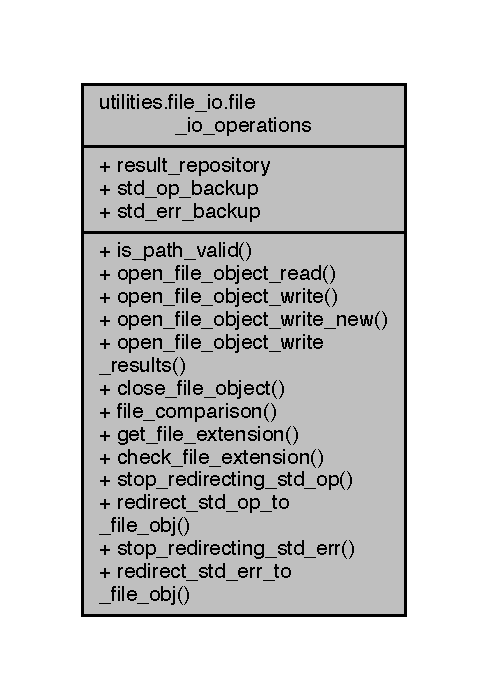
\includegraphics[width=234pt]{db/d83/classutilities_1_1file__io_1_1file__io__operations__coll__graph}
\end{center}
\end{figure}
\subsection*{Static Public Member Functions}
\begin{DoxyCompactItemize}
\item 
def \hyperlink{classutilities_1_1file__io_1_1file__io__operations_a5c4be751037b1ba20bb57884b93e7445}{is\+\_\+path\+\_\+valid} (filename)
\begin{DoxyCompactList}\small\item\em Method to check if a path to file is valid. \end{DoxyCompactList}\item 
def \hyperlink{classutilities_1_1file__io_1_1file__io__operations_a1a7ef324955033ad370338fe37e68194}{open\+\_\+file\+\_\+object\+\_\+read} (filename)
\begin{DoxyCompactList}\small\item\em Method to open a file object for read/input operations. \end{DoxyCompactList}\item 
def \hyperlink{classutilities_1_1file__io_1_1file__io__operations_aaf94e26da1d988ece479d1600ad1de4a}{open\+\_\+file\+\_\+object\+\_\+write} (filename)
\begin{DoxyCompactList}\small\item\em Method to open a file object for write/output operations. \end{DoxyCompactList}\item 
def \hyperlink{classutilities_1_1file__io_1_1file__io__operations_aefa9041777265e5066f9f5a48fb5a21e}{open\+\_\+file\+\_\+object\+\_\+write\+\_\+new} (filename)
\begin{DoxyCompactList}\small\item\em Method to open a new file object for write/output operations. \end{DoxyCompactList}\item 
def \hyperlink{classutilities_1_1file__io_1_1file__io__operations_ad091638ea961413dba6775d065c0d589}{open\+\_\+file\+\_\+object\+\_\+write\+\_\+results} ()
\begin{DoxyCompactList}\small\item\em Method to open a new file object for write/output operations to store simulation and/or experimental results. \end{DoxyCompactList}\item 
def \hyperlink{classutilities_1_1file__io_1_1file__io__operations_a15cce5bd7767b057cdc569f393c24866}{close\+\_\+file\+\_\+object} (file\+\_\+obj)
\begin{DoxyCompactList}\small\item\em Method to close a file object. \end{DoxyCompactList}\item 
def \hyperlink{classutilities_1_1file__io_1_1file__io__operations_a9b3808ff6b165f5e73b780036f73a917}{file\+\_\+comparison} (file1, file2)
\begin{DoxyCompactList}\small\item\em Method to determine if two files are equivalent. \end{DoxyCompactList}\item 
def \hyperlink{classutilities_1_1file__io_1_1file__io__operations_a7e3cbb46884ca64a14cd367b1e625082}{get\+\_\+file\+\_\+extension} (filename)
\begin{DoxyCompactList}\small\item\em Method to determine the file extension of a file. \end{DoxyCompactList}\item 
def \hyperlink{classutilities_1_1file__io_1_1file__io__operations_a902e9fd0dc0da35e3b374deae44051c6}{check\+\_\+file\+\_\+extension} (filename, file\+\_\+extension)
\begin{DoxyCompactList}\small\item\em Method to determine if the file extension of a file matches with a given file extension. \end{DoxyCompactList}\item 
def \hyperlink{classutilities_1_1file__io_1_1file__io__operations_afc81e06fe5b168f0ca2baf3f3cf5f449}{stop\+\_\+redirecting\+\_\+std\+\_\+op} ()
\begin{DoxyCompactList}\small\item\em Method to end redirection of standard output. \end{DoxyCompactList}\item 
def \hyperlink{classutilities_1_1file__io_1_1file__io__operations_a9ebd9b8cca3921274c4777ec7073c23f}{redirect\+\_\+std\+\_\+op\+\_\+to\+\_\+file\+\_\+obj} (file\+\_\+obj)
\begin{DoxyCompactList}\small\item\em Method to redirect standard output to a file object with write access. \end{DoxyCompactList}\item 
def \hyperlink{classutilities_1_1file__io_1_1file__io__operations_abc05dc3f53dc62bfe62aa316219b9807}{stop\+\_\+redirecting\+\_\+std\+\_\+err} ()
\begin{DoxyCompactList}\small\item\em Method to end redirection of standard error. \end{DoxyCompactList}\item 
def \hyperlink{classutilities_1_1file__io_1_1file__io__operations_a992b70cc7eeaafbe03fe5deb6a9f95d5}{redirect\+\_\+std\+\_\+err\+\_\+to\+\_\+file\+\_\+obj} (file\+\_\+obj)
\begin{DoxyCompactList}\small\item\em Method to redirect standard error to a file object with write access. \end{DoxyCompactList}\end{DoxyCompactItemize}
\subsection*{Static Public Attributes}
\begin{DoxyCompactItemize}
\item 
string \hyperlink{classutilities_1_1file__io_1_1file__io__operations_a7d92fe3b9053aa784ce73062bed07bd5}{result\+\_\+repository} = \char`\"{}/Users/zhiyang/Documents/ricerca/risultati\+\_\+sperimentali/std-\/cell-\/library-\/characterization\char`\"{}
\item 
\hyperlink{classutilities_1_1file__io_1_1file__io__operations_ae84964a620a018ec377b7e53f241dbf7}{std\+\_\+op\+\_\+backup} = None
\item 
\hyperlink{classutilities_1_1file__io_1_1file__io__operations_a979e9173080e7b88f0c296409a26ac01}{std\+\_\+err\+\_\+backup} = None
\end{DoxyCompactItemize}


\subsection{Detailed Description}
Module with methods that perform file I/\+O operations. 

\begin{DoxyVerb}    Location to store simulation and/or experimental results.
    Requires an absolute path, since no processing will be done
        to check if this is an absolute path or relative path.
\end{DoxyVerb}
 

Definition at line \hyperlink{file__io_8py_source_l00097}{97} of file \hyperlink{file__io_8py_source}{file\+\_\+io.\+py}.



\subsection{Member Function Documentation}
\hypertarget{classutilities_1_1file__io_1_1file__io__operations_a902e9fd0dc0da35e3b374deae44051c6}{}\index{utilities\+::file\+\_\+io\+::file\+\_\+io\+\_\+operations@{utilities\+::file\+\_\+io\+::file\+\_\+io\+\_\+operations}!check\+\_\+file\+\_\+extension@{check\+\_\+file\+\_\+extension}}
\index{check\+\_\+file\+\_\+extension@{check\+\_\+file\+\_\+extension}!utilities\+::file\+\_\+io\+::file\+\_\+io\+\_\+operations@{utilities\+::file\+\_\+io\+::file\+\_\+io\+\_\+operations}}
\subsubsection[{check\+\_\+file\+\_\+extension(filename, file\+\_\+extension)}]{\setlength{\rightskip}{0pt plus 5cm}def utilities.\+file\+\_\+io.\+file\+\_\+io\+\_\+operations.\+check\+\_\+file\+\_\+extension (
\begin{DoxyParamCaption}
\item[{}]{filename, }
\item[{}]{file\+\_\+extension}
\end{DoxyParamCaption}
)\hspace{0.3cm}{\ttfamily [static]}}\label{classutilities_1_1file__io_1_1file__io__operations_a902e9fd0dc0da35e3b374deae44051c6}


Method to determine if the file extension of a file matches with a given file extension. 


\begin{DoxyParams}{Parameters}
{\em filename} & -\/ Name of a file. \\
\hline
{\em file\+\_\+extension} & -\/ Extension \\
\hline
\end{DoxyParams}
\begin{DoxyReturn}{Returns}
boolean True if the file extension of the given filename matches file\+\_\+extension; else, return False. O(n) method, with respect to the number of characters in the path\+\_\+to\+\_\+file argument; traverse the string from the right end till the first period is found (this indicates the file extension). 
\end{DoxyReturn}


Definition at line \hyperlink{file__io_8py_source_l00267}{267} of file \hyperlink{file__io_8py_source}{file\+\_\+io.\+py}.


\begin{DoxyCode}
\hypertarget{classutilities_1_1file__io_1_1file__io__operations_l00267}{}\hyperlink{classutilities_1_1file__io_1_1file__io__operations_a902e9fd0dc0da35e3b374deae44051c6}{00267}     \textcolor{keyword}{def }\hyperlink{classutilities_1_1file__io_1_1file__io__operations_a902e9fd0dc0da35e3b374deae44051c6}{check\_file\_extension}(filename, file\_extension):
00268         \textcolor{keywordflow}{if} file\_extension == file\_io\_operations.get\_file\_extension(filename):
00269             \textcolor{keywordflow}{return} \textcolor{keyword}{True}
00270         \textcolor{keywordflow}{else}:
00271             \textcolor{keywordflow}{return} \textcolor{keyword}{False}
\end{DoxyCode}
\hypertarget{classutilities_1_1file__io_1_1file__io__operations_a15cce5bd7767b057cdc569f393c24866}{}\index{utilities\+::file\+\_\+io\+::file\+\_\+io\+\_\+operations@{utilities\+::file\+\_\+io\+::file\+\_\+io\+\_\+operations}!close\+\_\+file\+\_\+object@{close\+\_\+file\+\_\+object}}
\index{close\+\_\+file\+\_\+object@{close\+\_\+file\+\_\+object}!utilities\+::file\+\_\+io\+::file\+\_\+io\+\_\+operations@{utilities\+::file\+\_\+io\+::file\+\_\+io\+\_\+operations}}
\subsubsection[{close\+\_\+file\+\_\+object(file\+\_\+obj)}]{\setlength{\rightskip}{0pt plus 5cm}def utilities.\+file\+\_\+io.\+file\+\_\+io\+\_\+operations.\+close\+\_\+file\+\_\+object (
\begin{DoxyParamCaption}
\item[{}]{file\+\_\+obj}
\end{DoxyParamCaption}
)\hspace{0.3cm}{\ttfamily [static]}}\label{classutilities_1_1file__io_1_1file__io__operations_a15cce5bd7767b057cdc569f393c24866}


Method to close a file object. 


\begin{DoxyParams}{Parameters}
{\em file\+\_\+obj} & -\/ A file object. \\
\hline
\end{DoxyParams}
\begin{DoxyReturn}{Returns}
-\/ Nothing. O(1) method. 
\end{DoxyReturn}


Definition at line \hyperlink{file__io_8py_source_l00219}{219} of file \hyperlink{file__io_8py_source}{file\+\_\+io.\+py}.


\begin{DoxyCode}
\hypertarget{classutilities_1_1file__io_1_1file__io__operations_l00219}{}\hyperlink{classutilities_1_1file__io_1_1file__io__operations_a15cce5bd7767b057cdc569f393c24866}{00219}     \textcolor{keyword}{def }\hyperlink{classutilities_1_1file__io_1_1file__io__operations_a15cce5bd7767b057cdc569f393c24866}{close\_file\_object}(file\_obj):
00220         file\_obj.close()
\end{DoxyCode}
\hypertarget{classutilities_1_1file__io_1_1file__io__operations_a9b3808ff6b165f5e73b780036f73a917}{}\index{utilities\+::file\+\_\+io\+::file\+\_\+io\+\_\+operations@{utilities\+::file\+\_\+io\+::file\+\_\+io\+\_\+operations}!file\+\_\+comparison@{file\+\_\+comparison}}
\index{file\+\_\+comparison@{file\+\_\+comparison}!utilities\+::file\+\_\+io\+::file\+\_\+io\+\_\+operations@{utilities\+::file\+\_\+io\+::file\+\_\+io\+\_\+operations}}
\subsubsection[{file\+\_\+comparison(file1, file2)}]{\setlength{\rightskip}{0pt plus 5cm}def utilities.\+file\+\_\+io.\+file\+\_\+io\+\_\+operations.\+file\+\_\+comparison (
\begin{DoxyParamCaption}
\item[{}]{file1, }
\item[{}]{file2}
\end{DoxyParamCaption}
)\hspace{0.3cm}{\ttfamily [static]}}\label{classutilities_1_1file__io_1_1file__io__operations_a9b3808ff6b165f5e73b780036f73a917}


Method to determine if two files are equivalent. 


\begin{DoxyParams}{Parameters}
{\em file1} & -\/ Path to a file. \\
\hline
{\em file2} & -\/ Path to another file. \\
\hline
\end{DoxyParams}
\begin{DoxyReturn}{Returns}
a boolean T\+R\+U\+E, if the files are equivalent. Else, return F\+A\+L\+S\+E. O(n) method, with respect to the number of lines in the larger (if the files are different), or either, of the files. 
\end{DoxyReturn}


Definition at line \hyperlink{file__io_8py_source_l00231}{231} of file \hyperlink{file__io_8py_source}{file\+\_\+io.\+py}.


\begin{DoxyCode}
\hypertarget{classutilities_1_1file__io_1_1file__io__operations_l00231}{}\hyperlink{classutilities_1_1file__io_1_1file__io__operations_a9b3808ff6b165f5e73b780036f73a917}{00231}     \textcolor{keyword}{def }\hyperlink{classutilities_1_1file__io_1_1file__io__operations_a9b3808ff6b165f5e73b780036f73a917}{file\_comparison}(file1, file2):
00232         \textcolor{keywordflow}{return} filecmp.cmp(file1,file2,shallow=\textcolor{keyword}{False})
\end{DoxyCode}
\hypertarget{classutilities_1_1file__io_1_1file__io__operations_a7e3cbb46884ca64a14cd367b1e625082}{}\index{utilities\+::file\+\_\+io\+::file\+\_\+io\+\_\+operations@{utilities\+::file\+\_\+io\+::file\+\_\+io\+\_\+operations}!get\+\_\+file\+\_\+extension@{get\+\_\+file\+\_\+extension}}
\index{get\+\_\+file\+\_\+extension@{get\+\_\+file\+\_\+extension}!utilities\+::file\+\_\+io\+::file\+\_\+io\+\_\+operations@{utilities\+::file\+\_\+io\+::file\+\_\+io\+\_\+operations}}
\subsubsection[{get\+\_\+file\+\_\+extension(filename)}]{\setlength{\rightskip}{0pt plus 5cm}def utilities.\+file\+\_\+io.\+file\+\_\+io\+\_\+operations.\+get\+\_\+file\+\_\+extension (
\begin{DoxyParamCaption}
\item[{}]{filename}
\end{DoxyParamCaption}
)\hspace{0.3cm}{\ttfamily [static]}}\label{classutilities_1_1file__io_1_1file__io__operations_a7e3cbb46884ca64a14cd367b1e625082}


Method to determine the file extension of a file. 


\begin{DoxyParams}{Parameters}
{\em filename} & -\/ Name of a file. \\
\hline
\end{DoxyParams}
\begin{DoxyReturn}{Returns}
the file extension of a file. O(n) method, with respect to the number of characters in the path\+\_\+to\+\_\+file argument; traverse the string from the right end till the first period is found (this indicates the file extension). References\+: 1) {\bfseries [Dharmkar2017]}\}{\bfseries [nosklo2017]}\} 2) 
\end{DoxyReturn}


Definition at line \hyperlink{file__io_8py_source_l00245}{245} of file \hyperlink{file__io_8py_source}{file\+\_\+io.\+py}.


\begin{DoxyCode}
\hypertarget{classutilities_1_1file__io_1_1file__io__operations_l00245}{}\hyperlink{classutilities_1_1file__io_1_1file__io__operations_a7e3cbb46884ca64a14cd367b1e625082}{00245}     \textcolor{keyword}{def }\hyperlink{classutilities_1_1file__io_1_1file__io__operations_a7e3cbb46884ca64a14cd367b1e625082}{get\_file\_extension}(filename):
00246         temp\_filename\_extension = \textcolor{stringliteral}{""}
00247         \textcolor{keywordflow}{while} \textcolor{keyword}{True}:
00248             filename\_prefix, filename\_extension = os.path.splitext(filename)
00249             \textcolor{keywordflow}{if} \textcolor{keywordflow}{not} filename\_extension:
00250                 \textcolor{keywordflow}{break}
00251             \textcolor{keywordflow}{else}:
00252                 filename  = filename\_prefix
00253                 temp\_filename\_extension = filename\_extension + temp\_filename\_extension
00254         \textcolor{keywordflow}{return} temp\_filename\_extension
\end{DoxyCode}
\hypertarget{classutilities_1_1file__io_1_1file__io__operations_a5c4be751037b1ba20bb57884b93e7445}{}\index{utilities\+::file\+\_\+io\+::file\+\_\+io\+\_\+operations@{utilities\+::file\+\_\+io\+::file\+\_\+io\+\_\+operations}!is\+\_\+path\+\_\+valid@{is\+\_\+path\+\_\+valid}}
\index{is\+\_\+path\+\_\+valid@{is\+\_\+path\+\_\+valid}!utilities\+::file\+\_\+io\+::file\+\_\+io\+\_\+operations@{utilities\+::file\+\_\+io\+::file\+\_\+io\+\_\+operations}}
\subsubsection[{is\+\_\+path\+\_\+valid(filename)}]{\setlength{\rightskip}{0pt plus 5cm}def utilities.\+file\+\_\+io.\+file\+\_\+io\+\_\+operations.\+is\+\_\+path\+\_\+valid (
\begin{DoxyParamCaption}
\item[{}]{filename}
\end{DoxyParamCaption}
)\hspace{0.3cm}{\ttfamily [static]}}\label{classutilities_1_1file__io_1_1file__io__operations_a5c4be751037b1ba20bb57884b93e7445}


Method to check if a path to file is valid. 


\begin{DoxyParams}{Parameters}
{\em filename} & -\/ Path to a file. \\
\hline
\end{DoxyParams}
\begin{DoxyReturn}{Returns}
a boolean T\+R\+U\+E, if the path to the file is valid. Else, return F\+A\+L\+S\+E. O(1) method. 
\end{DoxyReturn}


Definition at line \hyperlink{file__io_8py_source_l00117}{117} of file \hyperlink{file__io_8py_source}{file\+\_\+io.\+py}.


\begin{DoxyCode}
\hypertarget{classutilities_1_1file__io_1_1file__io__operations_l00117}{}\hyperlink{classutilities_1_1file__io_1_1file__io__operations_a5c4be751037b1ba20bb57884b93e7445}{00117}     \textcolor{keyword}{def }\hyperlink{classutilities_1_1file__io_1_1file__io__operations_a5c4be751037b1ba20bb57884b93e7445}{is\_path\_valid}(filename):
00118         \textcolor{keywordflow}{if} (os.path.exists(filename) \textcolor{keywordflow}{and} os.path.isfile(filename)):
00119             \textcolor{keywordflow}{return} \textcolor{keyword}{True}
00120         \textcolor{keywordflow}{else}:
00121             \textcolor{keywordflow}{return} \textcolor{keyword}{False}
\end{DoxyCode}
\hypertarget{classutilities_1_1file__io_1_1file__io__operations_a1a7ef324955033ad370338fe37e68194}{}\index{utilities\+::file\+\_\+io\+::file\+\_\+io\+\_\+operations@{utilities\+::file\+\_\+io\+::file\+\_\+io\+\_\+operations}!open\+\_\+file\+\_\+object\+\_\+read@{open\+\_\+file\+\_\+object\+\_\+read}}
\index{open\+\_\+file\+\_\+object\+\_\+read@{open\+\_\+file\+\_\+object\+\_\+read}!utilities\+::file\+\_\+io\+::file\+\_\+io\+\_\+operations@{utilities\+::file\+\_\+io\+::file\+\_\+io\+\_\+operations}}
\subsubsection[{open\+\_\+file\+\_\+object\+\_\+read(filename)}]{\setlength{\rightskip}{0pt plus 5cm}def utilities.\+file\+\_\+io.\+file\+\_\+io\+\_\+operations.\+open\+\_\+file\+\_\+object\+\_\+read (
\begin{DoxyParamCaption}
\item[{}]{filename}
\end{DoxyParamCaption}
)\hspace{0.3cm}{\ttfamily [static]}}\label{classutilities_1_1file__io_1_1file__io__operations_a1a7ef324955033ad370338fe37e68194}


Method to open a file object for read/input operations. 


\begin{DoxyParams}{Parameters}
{\em filename} & -\/ Path to a file. \\
\hline
\end{DoxyParams}
\begin{DoxyReturn}{Returns}
file object ip\+\_\+file\+\_\+obj 
\end{DoxyReturn}

\begin{DoxyExceptions}{Exceptions}
{\em Exception} & for invalid path to the file. O(1) method. \\
\hline
\end{DoxyExceptions}


Definition at line \hyperlink{file__io_8py_source_l00129}{129} of file \hyperlink{file__io_8py_source}{file\+\_\+io.\+py}.


\begin{DoxyCode}
\hypertarget{classutilities_1_1file__io_1_1file__io__operations_l00129}{}\hyperlink{classutilities_1_1file__io_1_1file__io__operations_a1a7ef324955033ad370338fe37e68194}{00129}     \textcolor{keyword}{def }\hyperlink{classutilities_1_1file__io_1_1file__io__operations_a1a7ef324955033ad370338fe37e68194}{open\_file\_object\_read}(filename):
00130         \textcolor{keywordflow}{if} file\_io\_operations.is\_path\_valid(filename):
00131             ip\_file\_obj = open(filename, \textcolor{stringliteral}{'}\textcolor{stringliteral}{r')}
00132 \textcolor{stringliteral}{            }\textcolor{keywordflow}{return} ip\_file\_obj
00133         \textcolor{keywordflow}{else}:
00134             \textcolor{keywordflow}{raise} Exception(\textcolor{stringliteral}{"File Read Operation: Path to file is invalid."})
\end{DoxyCode}
\hypertarget{classutilities_1_1file__io_1_1file__io__operations_aaf94e26da1d988ece479d1600ad1de4a}{}\index{utilities\+::file\+\_\+io\+::file\+\_\+io\+\_\+operations@{utilities\+::file\+\_\+io\+::file\+\_\+io\+\_\+operations}!open\+\_\+file\+\_\+object\+\_\+write@{open\+\_\+file\+\_\+object\+\_\+write}}
\index{open\+\_\+file\+\_\+object\+\_\+write@{open\+\_\+file\+\_\+object\+\_\+write}!utilities\+::file\+\_\+io\+::file\+\_\+io\+\_\+operations@{utilities\+::file\+\_\+io\+::file\+\_\+io\+\_\+operations}}
\subsubsection[{open\+\_\+file\+\_\+object\+\_\+write(filename)}]{\setlength{\rightskip}{0pt plus 5cm}def utilities.\+file\+\_\+io.\+file\+\_\+io\+\_\+operations.\+open\+\_\+file\+\_\+object\+\_\+write (
\begin{DoxyParamCaption}
\item[{}]{filename}
\end{DoxyParamCaption}
)\hspace{0.3cm}{\ttfamily [static]}}\label{classutilities_1_1file__io_1_1file__io__operations_aaf94e26da1d988ece479d1600ad1de4a}


Method to open a file object for write/output operations. 


\begin{DoxyParams}{Parameters}
{\em filename} & -\/ Path to a file. \\
\hline
\end{DoxyParams}
\begin{DoxyReturn}{Returns}
file object op\+\_\+file\+\_\+obj that enables writing to the file named \char`\"{}filename\char`\"{}. 
\end{DoxyReturn}

\begin{DoxyExceptions}{Exceptions}
{\em Exception} & for invalid path to the file. O(1) method. \\
\hline
\end{DoxyExceptions}


Definition at line \hyperlink{file__io_8py_source_l00143}{143} of file \hyperlink{file__io_8py_source}{file\+\_\+io.\+py}.


\begin{DoxyCode}
\hypertarget{classutilities_1_1file__io_1_1file__io__operations_l00143}{}\hyperlink{classutilities_1_1file__io_1_1file__io__operations_aaf94e26da1d988ece479d1600ad1de4a}{00143}     \textcolor{keyword}{def }\hyperlink{classutilities_1_1file__io_1_1file__io__operations_aaf94e26da1d988ece479d1600ad1de4a}{open\_file\_object\_write}(filename):
00144         \textcolor{keywordflow}{if} \textcolor{keywordflow}{not} file\_io\_operations.is\_path\_valid(filename):
00145             op\_file\_obj = open(filename, \textcolor{stringliteral}{'w'})
00146             \textcolor{keywordflow}{return} op\_file\_obj
00147         \textcolor{keywordflow}{else}:
00148             \textcolor{keywordflow}{raise} Exception(\textcolor{stringliteral}{"File Write Operation: Path to file is valid."})
\end{DoxyCode}
\hypertarget{classutilities_1_1file__io_1_1file__io__operations_aefa9041777265e5066f9f5a48fb5a21e}{}\index{utilities\+::file\+\_\+io\+::file\+\_\+io\+\_\+operations@{utilities\+::file\+\_\+io\+::file\+\_\+io\+\_\+operations}!open\+\_\+file\+\_\+object\+\_\+write\+\_\+new@{open\+\_\+file\+\_\+object\+\_\+write\+\_\+new}}
\index{open\+\_\+file\+\_\+object\+\_\+write\+\_\+new@{open\+\_\+file\+\_\+object\+\_\+write\+\_\+new}!utilities\+::file\+\_\+io\+::file\+\_\+io\+\_\+operations@{utilities\+::file\+\_\+io\+::file\+\_\+io\+\_\+operations}}
\subsubsection[{open\+\_\+file\+\_\+object\+\_\+write\+\_\+new(filename)}]{\setlength{\rightskip}{0pt plus 5cm}def utilities.\+file\+\_\+io.\+file\+\_\+io\+\_\+operations.\+open\+\_\+file\+\_\+object\+\_\+write\+\_\+new (
\begin{DoxyParamCaption}
\item[{}]{filename}
\end{DoxyParamCaption}
)\hspace{0.3cm}{\ttfamily [static]}}\label{classutilities_1_1file__io_1_1file__io__operations_aefa9041777265e5066f9f5a48fb5a21e}


Method to open a new file object for write/output operations. 


\begin{DoxyParams}{Parameters}
{\em filename} & -\/ Path to a file. \\
\hline
\end{DoxyParams}
\begin{DoxyReturn}{Returns}
file object op\+\_\+file\+\_\+obj that enables writing to the file named \char`\"{}filename\char`\"{}. O(1) method. 
\end{DoxyReturn}


Definition at line \hyperlink{file__io_8py_source_l00156}{156} of file \hyperlink{file__io_8py_source}{file\+\_\+io.\+py}.


\begin{DoxyCode}
\hypertarget{classutilities_1_1file__io_1_1file__io__operations_l00156}{}\hyperlink{classutilities_1_1file__io_1_1file__io__operations_aefa9041777265e5066f9f5a48fb5a21e}{00156}     \textcolor{keyword}{def }\hyperlink{classutilities_1_1file__io_1_1file__io__operations_aefa9041777265e5066f9f5a48fb5a21e}{open\_file\_object\_write\_new}(filename):
00157         \textcolor{keywordflow}{if} file\_io\_operations.is\_path\_valid(filename):
00158             os.remove(filename)
00159         op\_file\_obj = open(filename, \textcolor{stringliteral}{'w'})
00160         \textcolor{keywordflow}{return} op\_file\_obj
\end{DoxyCode}
\hypertarget{classutilities_1_1file__io_1_1file__io__operations_ad091638ea961413dba6775d065c0d589}{}\index{utilities\+::file\+\_\+io\+::file\+\_\+io\+\_\+operations@{utilities\+::file\+\_\+io\+::file\+\_\+io\+\_\+operations}!open\+\_\+file\+\_\+object\+\_\+write\+\_\+results@{open\+\_\+file\+\_\+object\+\_\+write\+\_\+results}}
\index{open\+\_\+file\+\_\+object\+\_\+write\+\_\+results@{open\+\_\+file\+\_\+object\+\_\+write\+\_\+results}!utilities\+::file\+\_\+io\+::file\+\_\+io\+\_\+operations@{utilities\+::file\+\_\+io\+::file\+\_\+io\+\_\+operations}}
\subsubsection[{open\+\_\+file\+\_\+object\+\_\+write\+\_\+results()}]{\setlength{\rightskip}{0pt plus 5cm}def utilities.\+file\+\_\+io.\+file\+\_\+io\+\_\+operations.\+open\+\_\+file\+\_\+object\+\_\+write\+\_\+results (
\begin{DoxyParamCaption}
{}
\end{DoxyParamCaption}
)\hspace{0.3cm}{\ttfamily [static]}}\label{classutilities_1_1file__io_1_1file__io__operations_ad091638ea961413dba6775d065c0d589}


Method to open a new file object for write/output operations to store simulation and/or experimental results. 


\begin{DoxyParams}{Parameters}
{\em -\/} & None. \\
\hline
\end{DoxyParams}
\begin{DoxyReturn}{Returns}
file object \char`\"{}results\+\_\+file\+\_\+obj\char`\"{} that writes data containing simulation and/or experimental results. O(1) method. 
\end{DoxyReturn}


Definition at line \hyperlink{file__io_8py_source_l00169}{169} of file \hyperlink{file__io_8py_source}{file\+\_\+io.\+py}.


\begin{DoxyCode}
\hypertarget{classutilities_1_1file__io_1_1file__io__operations_l00169}{}\hyperlink{classutilities_1_1file__io_1_1file__io__operations_ad091638ea961413dba6775d065c0d589}{00169}     \textcolor{keyword}{def }\hyperlink{classutilities_1_1file__io_1_1file__io__operations_ad091638ea961413dba6775d065c0d589}{open\_file\_object\_write\_results}():
00170         \textcolor{comment}{# Determine path to store simulation/experimental results.}
00171         results\_filename = generate\_filename.create\_filename()
00172         \textcolor{comment}{# Tokenize this filename (DD-MM-YY-HR-MN-SS-US format).}
00173         tokens = date\_time\_operations.get\_date\_time\_tokens\_of\_filename(results\_filename)
00174         \textcolor{comment}{# Determine which year should the results file be placed in.}
00175         current\_path = os.path.join(file\_io\_operations.result\_repository,tokens[2])
00176         \textcolor{comment}{#if (os.path.exists(current\_path) and os.path.isdir(current\_path)):}
00177         \textcolor{keywordflow}{if} os.path.isdir(current\_path):
00178             \textcolor{comment}{# Determine which month should the results file be placed in.}
00179             \textcolor{comment}{#print("tokens[1]=",tokens[1],"=")}
00180             \textcolor{comment}{
      #print("date\_time\_operations.mth\_number\_name[tokens[1]]=",date\_time\_operations.mth\_number\_name[tokens[1]],"=")}
00181             current\_path = os.path.join(current\_path,date\_time\_operations.mth\_number\_name[tokens[1]])
00182             \textcolor{keywordflow}{if} \textcolor{keywordflow}{not} os.path.isdir(current\_path):
00183                 print(\textcolor{stringliteral}{" ... Creating directory for month at:"},current\_path)
00184                 \textcolor{keywordflow}{try}:
00185                     \textcolor{comment}{#os.mkdirs(current\_path, exist\_ok = True)}
00186                     os.makedirs(current\_path, exist\_ok = \textcolor{keyword}{True})
00187                 \textcolor{keywordflow}{except} OSError:
00188                     print(\textcolor{stringliteral}{"Encountered error in making directory."}, file=sys.stderr)
00189                     logging.error(\textcolor{stringliteral}{"Determine why directory for month cannot be created."})
00190             \textcolor{keywordflow}{else}:
00191                 print(current\_path,\textcolor{stringliteral}{"=works= ... From: file\_io.py, line 146."})
00192         \textcolor{keywordflow}{else}:
00193             print(\textcolor{stringliteral}{" ... Creating directory for year at:"},current\_path)
00194             \textcolor{keywordflow}{try}:
00195                 \textcolor{comment}{#os.mkdirs(current\_path, exist\_ok = True)}
00196                 os.makedirs(current\_path, exist\_ok = \textcolor{keyword}{True})
00197             \textcolor{keywordflow}{except} OSError:
00198                 print(\textcolor{stringliteral}{"Encountered error in making directory."}, file=sys.stderr)
00199                 logging.error(\textcolor{stringliteral}{"Determine why directory for year cannot be created."})
00200             \textcolor{comment}{# Determine which month should the results file be placed in.}
00201             current\_path = os.path.join(current\_path, date\_time\_operations.mth\_number\_name[tokens[1]])
00202             print(\textcolor{stringliteral}{" ...os.path.exists(current\_path:"},os.path.exists(current\_path))
00203             print(\textcolor{stringliteral}{" ...os.path.isdir(current\_path):"},os.path.isdir(current\_path))
00204             print(\textcolor{stringliteral}{" ... Creating directory for month at:"},current\_path)
00205             \textcolor{keywordflow}{try}:
00206                 \textcolor{comment}{#os.mkdirs(current\_path, exist\_ok = True)}
00207                 os.makedirs(current\_path, exist\_ok = \textcolor{keyword}{True})
00208             \textcolor{keywordflow}{except} OSError:
00209                 print(\textcolor{stringliteral}{"Encountered error in making directory."}, file=sys.stderr)
00210                 logging.error(\textcolor{stringliteral}{"Determine why directory for month cannot be created."})
00211         results\_filename = os.path.join(current\_path, results\_filename)
00212         \textcolor{keywordflow}{return} file\_io\_operations.open\_file\_object\_write(results\_filename)
\end{DoxyCode}
\hypertarget{classutilities_1_1file__io_1_1file__io__operations_a992b70cc7eeaafbe03fe5deb6a9f95d5}{}\index{utilities\+::file\+\_\+io\+::file\+\_\+io\+\_\+operations@{utilities\+::file\+\_\+io\+::file\+\_\+io\+\_\+operations}!redirect\+\_\+std\+\_\+err\+\_\+to\+\_\+file\+\_\+obj@{redirect\+\_\+std\+\_\+err\+\_\+to\+\_\+file\+\_\+obj}}
\index{redirect\+\_\+std\+\_\+err\+\_\+to\+\_\+file\+\_\+obj@{redirect\+\_\+std\+\_\+err\+\_\+to\+\_\+file\+\_\+obj}!utilities\+::file\+\_\+io\+::file\+\_\+io\+\_\+operations@{utilities\+::file\+\_\+io\+::file\+\_\+io\+\_\+operations}}
\subsubsection[{redirect\+\_\+std\+\_\+err\+\_\+to\+\_\+file\+\_\+obj(file\+\_\+obj)}]{\setlength{\rightskip}{0pt plus 5cm}def utilities.\+file\+\_\+io.\+file\+\_\+io\+\_\+operations.\+redirect\+\_\+std\+\_\+err\+\_\+to\+\_\+file\+\_\+obj (
\begin{DoxyParamCaption}
\item[{}]{file\+\_\+obj}
\end{DoxyParamCaption}
)\hspace{0.3cm}{\ttfamily [static]}}\label{classutilities_1_1file__io_1_1file__io__operations_a992b70cc7eeaafbe03fe5deb6a9f95d5}


Method to redirect standard error to a file object with write access. 


\begin{DoxyParams}{Parameters}
{\em file\+\_\+obj} & -\/ File object with write access. \\
\hline
\end{DoxyParams}
\begin{DoxyReturn}{Returns}
boolean True if standard error is redirected to a file object with write access; else, return False. O(1) method. 
\end{DoxyReturn}


Definition at line \hyperlink{file__io_8py_source_l00307}{307} of file \hyperlink{file__io_8py_source}{file\+\_\+io.\+py}.


\begin{DoxyCode}
\hypertarget{classutilities_1_1file__io_1_1file__io__operations_l00307}{}\hyperlink{classutilities_1_1file__io_1_1file__io__operations_a992b70cc7eeaafbe03fe5deb6a9f95d5}{00307}     \textcolor{keyword}{def }\hyperlink{classutilities_1_1file__io_1_1file__io__operations_a992b70cc7eeaafbe03fe5deb6a9f95d5}{redirect\_std\_err\_to\_file\_obj}(file\_obj):
00308         file\_io\_operations.std\_err\_backup = sys.stderr
00309         sys.stderr = file\_obj
00310 \end{DoxyCode}
\hypertarget{classutilities_1_1file__io_1_1file__io__operations_a9ebd9b8cca3921274c4777ec7073c23f}{}\index{utilities\+::file\+\_\+io\+::file\+\_\+io\+\_\+operations@{utilities\+::file\+\_\+io\+::file\+\_\+io\+\_\+operations}!redirect\+\_\+std\+\_\+op\+\_\+to\+\_\+file\+\_\+obj@{redirect\+\_\+std\+\_\+op\+\_\+to\+\_\+file\+\_\+obj}}
\index{redirect\+\_\+std\+\_\+op\+\_\+to\+\_\+file\+\_\+obj@{redirect\+\_\+std\+\_\+op\+\_\+to\+\_\+file\+\_\+obj}!utilities\+::file\+\_\+io\+::file\+\_\+io\+\_\+operations@{utilities\+::file\+\_\+io\+::file\+\_\+io\+\_\+operations}}
\subsubsection[{redirect\+\_\+std\+\_\+op\+\_\+to\+\_\+file\+\_\+obj(file\+\_\+obj)}]{\setlength{\rightskip}{0pt plus 5cm}def utilities.\+file\+\_\+io.\+file\+\_\+io\+\_\+operations.\+redirect\+\_\+std\+\_\+op\+\_\+to\+\_\+file\+\_\+obj (
\begin{DoxyParamCaption}
\item[{}]{file\+\_\+obj}
\end{DoxyParamCaption}
)\hspace{0.3cm}{\ttfamily [static]}}\label{classutilities_1_1file__io_1_1file__io__operations_a9ebd9b8cca3921274c4777ec7073c23f}


Method to redirect standard output to a file object with write access. 


\begin{DoxyParams}{Parameters}
{\em file\+\_\+obj} & -\/ File object with write access. \\
\hline
\end{DoxyParams}
\begin{DoxyReturn}{Returns}
boolean True if standard output is redirected to a file object with write access; else, return False. O(1) method. 
\end{DoxyReturn}


Definition at line \hyperlink{file__io_8py_source_l00288}{288} of file \hyperlink{file__io_8py_source}{file\+\_\+io.\+py}.


\begin{DoxyCode}
\hypertarget{classutilities_1_1file__io_1_1file__io__operations_l00288}{}\hyperlink{classutilities_1_1file__io_1_1file__io__operations_a9ebd9b8cca3921274c4777ec7073c23f}{00288}     \textcolor{keyword}{def }\hyperlink{classutilities_1_1file__io_1_1file__io__operations_a9ebd9b8cca3921274c4777ec7073c23f}{redirect\_std\_op\_to\_file\_obj}(file\_obj):
00289         file\_io\_operations.std\_op\_backup = sys.stdout
00290         sys.stdout = file\_obj
\end{DoxyCode}
\hypertarget{classutilities_1_1file__io_1_1file__io__operations_abc05dc3f53dc62bfe62aa316219b9807}{}\index{utilities\+::file\+\_\+io\+::file\+\_\+io\+\_\+operations@{utilities\+::file\+\_\+io\+::file\+\_\+io\+\_\+operations}!stop\+\_\+redirecting\+\_\+std\+\_\+err@{stop\+\_\+redirecting\+\_\+std\+\_\+err}}
\index{stop\+\_\+redirecting\+\_\+std\+\_\+err@{stop\+\_\+redirecting\+\_\+std\+\_\+err}!utilities\+::file\+\_\+io\+::file\+\_\+io\+\_\+operations@{utilities\+::file\+\_\+io\+::file\+\_\+io\+\_\+operations}}
\subsubsection[{stop\+\_\+redirecting\+\_\+std\+\_\+err()}]{\setlength{\rightskip}{0pt plus 5cm}def utilities.\+file\+\_\+io.\+file\+\_\+io\+\_\+operations.\+stop\+\_\+redirecting\+\_\+std\+\_\+err (
\begin{DoxyParamCaption}
{}
\end{DoxyParamCaption}
)\hspace{0.3cm}{\ttfamily [static]}}\label{classutilities_1_1file__io_1_1file__io__operations_abc05dc3f53dc62bfe62aa316219b9807}


Method to end redirection of standard error. 


\begin{DoxyParams}{Parameters}
{\em -\/} & None. \\
\hline
\end{DoxyParams}
\begin{DoxyReturn}{Returns}
-\/ Nothing. O(1) method. 
\end{DoxyReturn}


Definition at line \hyperlink{file__io_8py_source_l00297}{297} of file \hyperlink{file__io_8py_source}{file\+\_\+io.\+py}.


\begin{DoxyCode}
\hypertarget{classutilities_1_1file__io_1_1file__io__operations_l00297}{}\hyperlink{classutilities_1_1file__io_1_1file__io__operations_abc05dc3f53dc62bfe62aa316219b9807}{00297}     \textcolor{keyword}{def }\hyperlink{classutilities_1_1file__io_1_1file__io__operations_abc05dc3f53dc62bfe62aa316219b9807}{stop\_redirecting\_std\_err}():
00298         sys.stderr = file\_io\_operations.std\_err\_backup
\end{DoxyCode}
\hypertarget{classutilities_1_1file__io_1_1file__io__operations_afc81e06fe5b168f0ca2baf3f3cf5f449}{}\index{utilities\+::file\+\_\+io\+::file\+\_\+io\+\_\+operations@{utilities\+::file\+\_\+io\+::file\+\_\+io\+\_\+operations}!stop\+\_\+redirecting\+\_\+std\+\_\+op@{stop\+\_\+redirecting\+\_\+std\+\_\+op}}
\index{stop\+\_\+redirecting\+\_\+std\+\_\+op@{stop\+\_\+redirecting\+\_\+std\+\_\+op}!utilities\+::file\+\_\+io\+::file\+\_\+io\+\_\+operations@{utilities\+::file\+\_\+io\+::file\+\_\+io\+\_\+operations}}
\subsubsection[{stop\+\_\+redirecting\+\_\+std\+\_\+op()}]{\setlength{\rightskip}{0pt plus 5cm}def utilities.\+file\+\_\+io.\+file\+\_\+io\+\_\+operations.\+stop\+\_\+redirecting\+\_\+std\+\_\+op (
\begin{DoxyParamCaption}
{}
\end{DoxyParamCaption}
)\hspace{0.3cm}{\ttfamily [static]}}\label{classutilities_1_1file__io_1_1file__io__operations_afc81e06fe5b168f0ca2baf3f3cf5f449}


Method to end redirection of standard output. 


\begin{DoxyParams}{Parameters}
{\em -\/} & None. \\
\hline
\end{DoxyParams}
\begin{DoxyReturn}{Returns}
-\/ Nothing. O(1) method. 
\end{DoxyReturn}


Definition at line \hyperlink{file__io_8py_source_l00278}{278} of file \hyperlink{file__io_8py_source}{file\+\_\+io.\+py}.


\begin{DoxyCode}
\hypertarget{classutilities_1_1file__io_1_1file__io__operations_l00278}{}\hyperlink{classutilities_1_1file__io_1_1file__io__operations_afc81e06fe5b168f0ca2baf3f3cf5f449}{00278}     \textcolor{keyword}{def }\hyperlink{classutilities_1_1file__io_1_1file__io__operations_afc81e06fe5b168f0ca2baf3f3cf5f449}{stop\_redirecting\_std\_op}():
00279         sys.stdout = file\_io\_operations.std\_op\_backup
\end{DoxyCode}


\subsection{Member Data Documentation}
\hypertarget{classutilities_1_1file__io_1_1file__io__operations_a7d92fe3b9053aa784ce73062bed07bd5}{}\index{utilities\+::file\+\_\+io\+::file\+\_\+io\+\_\+operations@{utilities\+::file\+\_\+io\+::file\+\_\+io\+\_\+operations}!result\+\_\+repository@{result\+\_\+repository}}
\index{result\+\_\+repository@{result\+\_\+repository}!utilities\+::file\+\_\+io\+::file\+\_\+io\+\_\+operations@{utilities\+::file\+\_\+io\+::file\+\_\+io\+\_\+operations}}
\subsubsection[{result\+\_\+repository}]{\setlength{\rightskip}{0pt plus 5cm}string utilities.\+file\+\_\+io.\+file\+\_\+io\+\_\+operations.\+result\+\_\+repository = \char`\"{}/Users/zhiyang/Documents/ricerca/risultati\+\_\+sperimentali/std-\/cell-\/library-\/characterization\char`\"{}\hspace{0.3cm}{\ttfamily [static]}}\label{classutilities_1_1file__io_1_1file__io__operations_a7d92fe3b9053aa784ce73062bed07bd5}


Definition at line \hyperlink{file__io_8py_source_l00104}{104} of file \hyperlink{file__io_8py_source}{file\+\_\+io.\+py}.

\hypertarget{classutilities_1_1file__io_1_1file__io__operations_a979e9173080e7b88f0c296409a26ac01}{}\index{utilities\+::file\+\_\+io\+::file\+\_\+io\+\_\+operations@{utilities\+::file\+\_\+io\+::file\+\_\+io\+\_\+operations}!std\+\_\+err\+\_\+backup@{std\+\_\+err\+\_\+backup}}
\index{std\+\_\+err\+\_\+backup@{std\+\_\+err\+\_\+backup}!utilities\+::file\+\_\+io\+::file\+\_\+io\+\_\+operations@{utilities\+::file\+\_\+io\+::file\+\_\+io\+\_\+operations}}
\subsubsection[{std\+\_\+err\+\_\+backup}]{\setlength{\rightskip}{0pt plus 5cm}utilities.\+file\+\_\+io.\+file\+\_\+io\+\_\+operations.\+std\+\_\+err\+\_\+backup = None\hspace{0.3cm}{\ttfamily [static]}}\label{classutilities_1_1file__io_1_1file__io__operations_a979e9173080e7b88f0c296409a26ac01}


Definition at line \hyperlink{file__io_8py_source_l00108}{108} of file \hyperlink{file__io_8py_source}{file\+\_\+io.\+py}.

\hypertarget{classutilities_1_1file__io_1_1file__io__operations_ae84964a620a018ec377b7e53f241dbf7}{}\index{utilities\+::file\+\_\+io\+::file\+\_\+io\+\_\+operations@{utilities\+::file\+\_\+io\+::file\+\_\+io\+\_\+operations}!std\+\_\+op\+\_\+backup@{std\+\_\+op\+\_\+backup}}
\index{std\+\_\+op\+\_\+backup@{std\+\_\+op\+\_\+backup}!utilities\+::file\+\_\+io\+::file\+\_\+io\+\_\+operations@{utilities\+::file\+\_\+io\+::file\+\_\+io\+\_\+operations}}
\subsubsection[{std\+\_\+op\+\_\+backup}]{\setlength{\rightskip}{0pt plus 5cm}utilities.\+file\+\_\+io.\+file\+\_\+io\+\_\+operations.\+std\+\_\+op\+\_\+backup = None\hspace{0.3cm}{\ttfamily [static]}}\label{classutilities_1_1file__io_1_1file__io__operations_ae84964a620a018ec377b7e53f241dbf7}


Definition at line \hyperlink{file__io_8py_source_l00106}{106} of file \hyperlink{file__io_8py_source}{file\+\_\+io.\+py}.



The documentation for this class was generated from the following file\+:\begin{DoxyCompactItemize}
\item 
utilities/\hyperlink{file__io_8py}{file\+\_\+io.\+py}\end{DoxyCompactItemize}

\hypertarget{classutilities_1_1file__io__tester_1_1file__io__operations__tester}{}\section{utilities.\+file\+\_\+io\+\_\+tester.\+file\+\_\+io\+\_\+operations\+\_\+tester Class Reference}
\label{classutilities_1_1file__io__tester_1_1file__io__operations__tester}\index{utilities.\+file\+\_\+io\+\_\+tester.\+file\+\_\+io\+\_\+operations\+\_\+tester@{utilities.\+file\+\_\+io\+\_\+tester.\+file\+\_\+io\+\_\+operations\+\_\+tester}}


Collaboration diagram for utilities.\+file\+\_\+io\+\_\+tester.\+file\+\_\+io\+\_\+operations\+\_\+tester\+:
\nopagebreak
\begin{figure}[H]
\begin{center}
\leavevmode

\includegraphics[width=234pt]{d8/dec/classutilities_1_1file__io__tester_1_1file__io__operations__tester__coll__graph}
\end{center}
\end{figure}
\subsection*{Static Public Member Functions}
\begin{DoxyCompactItemize}
\item 
def \hyperlink{classutilities_1_1file__io__tester_1_1file__io__operations__tester_a847cc701af96fbf9558cdae859f379d6}{test\+\_\+file\+\_\+io\+\_\+operations\+\_\+with\+\_\+invalid\+\_\+file} ()
\begin{DoxyCompactList}\small\item\em ========================================================= Method to test the methods that perform file I/\+O operations with an invalid file. \end{DoxyCompactList}\item 
def \hyperlink{classutilities_1_1file__io__tester_1_1file__io__operations__tester_a9683b5a406697686900d28455bd3d5c3}{test\+\_\+file\+\_\+io\+\_\+operations\+\_\+with\+\_\+valid\+\_\+file} ()
\begin{DoxyCompactList}\small\item\em ========================================================= Method to test the methods that perform file I/\+O operations with a valid file. \end{DoxyCompactList}\item 
def \hyperlink{classutilities_1_1file__io__tester_1_1file__io__operations__tester_a5efc5f988841df586d1db5619d5fe49e}{test\+\_\+file\+\_\+io\+\_\+operations\+\_\+on\+\_\+files\+\_\+with\+\_\+same\+\_\+content} ()
\begin{DoxyCompactList}\small\item\em ========================================================= Method to test file operations on files with the same content. \end{DoxyCompactList}\item 
def \hyperlink{classutilities_1_1file__io__tester_1_1file__io__operations__tester_a264a387fe5693619617b8b10be1354af}{test\+\_\+file\+\_\+io\+\_\+operations\+\_\+get\+\_\+file\+\_\+extension} ()
\begin{DoxyCompactList}\small\item\em ========================================================= Method to test \hyperlink{classutilities_1_1file__io_1_1file__io__operations_a7e3cbb46884ca64a14cd367b1e625082}{file\+\_\+io\+\_\+operations.\+get\+\_\+file\+\_\+extension()} method. \end{DoxyCompactList}\item 
def \hyperlink{classutilities_1_1file__io__tester_1_1file__io__operations__tester_aeacc9602a024e8f2b6701b9305ffc930}{test\+\_\+file\+\_\+io\+\_\+operations\+\_\+check\+\_\+file\+\_\+extension} ()
\begin{DoxyCompactList}\small\item\em ========================================================= Method to test \hyperlink{classutilities_1_1file__io_1_1file__io__operations_a902e9fd0dc0da35e3b374deae44051c6}{file\+\_\+io\+\_\+operations.\+check\+\_\+file\+\_\+extension()} method. \end{DoxyCompactList}\item 
def \hyperlink{classutilities_1_1file__io__tester_1_1file__io__operations__tester_a7fa460b989d5a77396a182df39255eba}{test\+\_\+file\+\_\+io\+\_\+operations\+\_\+open\+\_\+file\+\_\+object\+\_\+write\+\_\+results} ()
\begin{DoxyCompactList}\small\item\em ========================================================= Method to test \hyperlink{classutilities_1_1file__io_1_1file__io__operations_ad091638ea961413dba6775d065c0d589}{file\+\_\+io\+\_\+operations.\+open\+\_\+file\+\_\+object\+\_\+write\+\_\+results()} method. \end{DoxyCompactList}\item 
def \hyperlink{classutilities_1_1file__io__tester_1_1file__io__operations__tester_a874961b1543ff59a1b1ea4b40abca8d2}{test\+\_\+file\+\_\+io\+\_\+operations} ()
\begin{DoxyCompactList}\small\item\em ========================================================= Method to test the methods that perform file I/\+O operations. \end{DoxyCompactList}\end{DoxyCompactItemize}


\subsection{Detailed Description}


Definition at line \hyperlink{file__io__tester_8py_source_l00089}{89} of file \hyperlink{file__io__tester_8py_source}{file\+\_\+io\+\_\+tester.\+py}.



\subsection{Member Function Documentation}
\hypertarget{classutilities_1_1file__io__tester_1_1file__io__operations__tester_a874961b1543ff59a1b1ea4b40abca8d2}{}\index{utilities\+::file\+\_\+io\+\_\+tester\+::file\+\_\+io\+\_\+operations\+\_\+tester@{utilities\+::file\+\_\+io\+\_\+tester\+::file\+\_\+io\+\_\+operations\+\_\+tester}!test\+\_\+file\+\_\+io\+\_\+operations@{test\+\_\+file\+\_\+io\+\_\+operations}}
\index{test\+\_\+file\+\_\+io\+\_\+operations@{test\+\_\+file\+\_\+io\+\_\+operations}!utilities\+::file\+\_\+io\+\_\+tester\+::file\+\_\+io\+\_\+operations\+\_\+tester@{utilities\+::file\+\_\+io\+\_\+tester\+::file\+\_\+io\+\_\+operations\+\_\+tester}}
\subsubsection[{test\+\_\+file\+\_\+io\+\_\+operations()}]{\setlength{\rightskip}{0pt plus 5cm}def utilities.\+file\+\_\+io\+\_\+tester.\+file\+\_\+io\+\_\+operations\+\_\+tester.\+test\+\_\+file\+\_\+io\+\_\+operations (
\begin{DoxyParamCaption}
{}
\end{DoxyParamCaption}
)\hspace{0.3cm}{\ttfamily [static]}}\label{classutilities_1_1file__io__tester_1_1file__io__operations__tester_a874961b1543ff59a1b1ea4b40abca8d2}


========================================================= Method to test the methods that perform file I/\+O operations. 

\begin{DoxyReturn}{Returns}
-\/ Nothing. O(1) method. 
\end{DoxyReturn}


Definition at line \hyperlink{file__io__tester_8py_source_l00283}{283} of file \hyperlink{file__io__tester_8py_source}{file\+\_\+io\+\_\+tester.\+py}.


\begin{DoxyCode}
\hypertarget{classutilities_1_1file__io__tester_1_1file__io__operations__tester_l00283}{}\hyperlink{classutilities_1_1file__io__tester_1_1file__io__operations__tester_a874961b1543ff59a1b1ea4b40abca8d2}{00283}     \textcolor{keyword}{def }\hyperlink{classutilities_1_1file__io__tester_1_1file__io__operations__tester_a874961b1543ff59a1b1ea4b40abca8d2}{test\_file\_io\_operations}():
00284         print(\textcolor{stringliteral}{"==   Testing class: file\_io\_operations."})
00285         file\_io\_operations\_tester.test\_file\_io\_operations\_with\_invalid\_file()
00286         file\_io\_operations\_tester.test\_file\_io\_operations\_with\_valid\_file()
00287         file\_io\_operations\_tester.test\_file\_io\_operations\_on\_files\_with\_same\_content()
00288         file\_io\_operations\_tester.test\_file\_io\_operations\_get\_file\_extension()
00289         file\_io\_operations\_tester.test\_file\_io\_operations\_check\_file\_extension()
00290         file\_io\_operations\_tester.test\_file\_io\_operations\_open\_file\_object\_write\_results()
00291 \end{DoxyCode}
\hypertarget{classutilities_1_1file__io__tester_1_1file__io__operations__tester_aeacc9602a024e8f2b6701b9305ffc930}{}\index{utilities\+::file\+\_\+io\+\_\+tester\+::file\+\_\+io\+\_\+operations\+\_\+tester@{utilities\+::file\+\_\+io\+\_\+tester\+::file\+\_\+io\+\_\+operations\+\_\+tester}!test\+\_\+file\+\_\+io\+\_\+operations\+\_\+check\+\_\+file\+\_\+extension@{test\+\_\+file\+\_\+io\+\_\+operations\+\_\+check\+\_\+file\+\_\+extension}}
\index{test\+\_\+file\+\_\+io\+\_\+operations\+\_\+check\+\_\+file\+\_\+extension@{test\+\_\+file\+\_\+io\+\_\+operations\+\_\+check\+\_\+file\+\_\+extension}!utilities\+::file\+\_\+io\+\_\+tester\+::file\+\_\+io\+\_\+operations\+\_\+tester@{utilities\+::file\+\_\+io\+\_\+tester\+::file\+\_\+io\+\_\+operations\+\_\+tester}}
\subsubsection[{test\+\_\+file\+\_\+io\+\_\+operations\+\_\+check\+\_\+file\+\_\+extension()}]{\setlength{\rightskip}{0pt plus 5cm}def utilities.\+file\+\_\+io\+\_\+tester.\+file\+\_\+io\+\_\+operations\+\_\+tester.\+test\+\_\+file\+\_\+io\+\_\+operations\+\_\+check\+\_\+file\+\_\+extension (
\begin{DoxyParamCaption}
{}
\end{DoxyParamCaption}
)\hspace{0.3cm}{\ttfamily [static]}}\label{classutilities_1_1file__io__tester_1_1file__io__operations__tester_aeacc9602a024e8f2b6701b9305ffc930}


========================================================= Method to test \hyperlink{classutilities_1_1file__io_1_1file__io__operations_a902e9fd0dc0da35e3b374deae44051c6}{file\+\_\+io\+\_\+operations.\+check\+\_\+file\+\_\+extension()} method. 

\begin{DoxyReturn}{Returns}
-\/ Nothing. O(1) method. 
\end{DoxyReturn}


Definition at line \hyperlink{file__io__tester_8py_source_l00245}{245} of file \hyperlink{file__io__tester_8py_source}{file\+\_\+io\+\_\+tester.\+py}.


\begin{DoxyCode}
\hypertarget{classutilities_1_1file__io__tester_1_1file__io__operations__tester_l00245}{}\hyperlink{classutilities_1_1file__io__tester_1_1file__io__operations__tester_aeacc9602a024e8f2b6701b9305ffc930}{00245}     \textcolor{keyword}{def }\hyperlink{classutilities_1_1file__io__tester_1_1file__io__operations__tester_aeacc9602a024e8f2b6701b9305ffc930}{test\_file\_io\_operations\_check\_file\_extension}():
00246         print(\textcolor{stringliteral}{" Testing file\_io\_operations.check\_file\_extension() method."})
00247         prompt = \textcolor{stringliteral}{"  ... Test: same file extension               \{\}"}
00248         statistical\_analysis.increment\_number\_test\_cases\_used()
00249         \textcolor{keywordflow}{if} file\_io\_operations.check\_file\_extension(\textcolor{stringliteral}{"something.text"},\textcolor{stringliteral}{".text"}):
00250             print(prompt .format(\textcolor{stringliteral}{"OK"}))
00251             statistical\_analysis.increment\_number\_test\_cases\_passed()
00252         \textcolor{keywordflow}{else}:
00253             print(prompt .format(\textcolor{stringliteral}{"FAIL!!!"}))
00254         prompt = \textcolor{stringliteral}{"  ... Test: different file extensions         \{\}"}
00255         statistical\_analysis.increment\_number\_test\_cases\_used()
00256         \textcolor{keywordflow}{if} \textcolor{keywordflow}{not} file\_io\_operations.check\_file\_extension(\textcolor{stringliteral}{"something.tar.gz"},\textcolor{stringliteral}{".rtsdtfyg"}):
00257             print(prompt .format(\textcolor{stringliteral}{"OK"}))
00258             statistical\_analysis.increment\_number\_test\_cases\_passed()
00259         \textcolor{keywordflow}{else}:
00260             print(prompt .format(\textcolor{stringliteral}{"FAIL!!!"}))
\end{DoxyCode}
\hypertarget{classutilities_1_1file__io__tester_1_1file__io__operations__tester_a264a387fe5693619617b8b10be1354af}{}\index{utilities\+::file\+\_\+io\+\_\+tester\+::file\+\_\+io\+\_\+operations\+\_\+tester@{utilities\+::file\+\_\+io\+\_\+tester\+::file\+\_\+io\+\_\+operations\+\_\+tester}!test\+\_\+file\+\_\+io\+\_\+operations\+\_\+get\+\_\+file\+\_\+extension@{test\+\_\+file\+\_\+io\+\_\+operations\+\_\+get\+\_\+file\+\_\+extension}}
\index{test\+\_\+file\+\_\+io\+\_\+operations\+\_\+get\+\_\+file\+\_\+extension@{test\+\_\+file\+\_\+io\+\_\+operations\+\_\+get\+\_\+file\+\_\+extension}!utilities\+::file\+\_\+io\+\_\+tester\+::file\+\_\+io\+\_\+operations\+\_\+tester@{utilities\+::file\+\_\+io\+\_\+tester\+::file\+\_\+io\+\_\+operations\+\_\+tester}}
\subsubsection[{test\+\_\+file\+\_\+io\+\_\+operations\+\_\+get\+\_\+file\+\_\+extension()}]{\setlength{\rightskip}{0pt plus 5cm}def utilities.\+file\+\_\+io\+\_\+tester.\+file\+\_\+io\+\_\+operations\+\_\+tester.\+test\+\_\+file\+\_\+io\+\_\+operations\+\_\+get\+\_\+file\+\_\+extension (
\begin{DoxyParamCaption}
{}
\end{DoxyParamCaption}
)\hspace{0.3cm}{\ttfamily [static]}}\label{classutilities_1_1file__io__tester_1_1file__io__operations__tester_a264a387fe5693619617b8b10be1354af}


========================================================= Method to test \hyperlink{classutilities_1_1file__io_1_1file__io__operations_a7e3cbb46884ca64a14cd367b1e625082}{file\+\_\+io\+\_\+operations.\+get\+\_\+file\+\_\+extension()} method. 

\begin{DoxyReturn}{Returns}
-\/ Nothing. O(1) method. 
\end{DoxyReturn}


Definition at line \hyperlink{file__io__tester_8py_source_l00216}{216} of file \hyperlink{file__io__tester_8py_source}{file\+\_\+io\+\_\+tester.\+py}.


\begin{DoxyCode}
\hypertarget{classutilities_1_1file__io__tester_1_1file__io__operations__tester_l00216}{}\hyperlink{classutilities_1_1file__io__tester_1_1file__io__operations__tester_a264a387fe5693619617b8b10be1354af}{00216}     \textcolor{keyword}{def }\hyperlink{classutilities_1_1file__io__tester_1_1file__io__operations__tester_a264a387fe5693619617b8b10be1354af}{test\_file\_io\_operations\_get\_file\_extension}():
00217         print(\textcolor{stringliteral}{" Testing file\_io\_operations.get\_file\_extension() method."})
00218         prompt = \textcolor{stringliteral}{"  ... Test: one file extension                \{\}"}
00219         statistical\_analysis.increment\_number\_test\_cases\_used()
00220         \textcolor{keywordflow}{if} file\_io\_operations.get\_file\_extension(\textcolor{stringliteral}{"something.text"}) == \textcolor{stringliteral}{".text"}:
00221             print(prompt .format(\textcolor{stringliteral}{"OK"}))
00222             statistical\_analysis.increment\_number\_test\_cases\_passed()
00223         \textcolor{keywordflow}{else}:
00224             print(prompt .format(\textcolor{stringliteral}{"FAIL!!!"}))
00225         prompt = \textcolor{stringliteral}{"  ... Test: double/dual file extensions           \{\}"}
00226         statistical\_analysis.increment\_number\_test\_cases\_used()
00227         \textcolor{keywordflow}{if} file\_io\_operations.get\_file\_extension(\textcolor{stringliteral}{"something.tar.gz"}) == \textcolor{stringliteral}{".tar.gz"}:
00228             print(prompt .format(\textcolor{stringliteral}{"OK"}))
00229             statistical\_analysis.increment\_number\_test\_cases\_passed()
00230         \textcolor{keywordflow}{else}:
00231             print(prompt .format(\textcolor{stringliteral}{"FAIL!!!"}))
00232             \textcolor{comment}{#print(file\_io\_operations.get\_file\_extension("something.tar.gz"))}
00233         prompt = \textcolor{stringliteral}{"  ... Test: multiple file extensions          \{\}"}
00234         statistical\_analysis.increment\_number\_test\_cases\_used()
00235         \textcolor{keywordflow}{if} file\_io\_operations.get\_file\_extension(\textcolor{stringliteral}{"something.pdf.tar.gz"}) == \textcolor{stringliteral}{".pdf.tar.gz"}:
00236             print(prompt .format(\textcolor{stringliteral}{"OK"}))
00237             statistical\_analysis.increment\_number\_test\_cases\_passed()
00238         \textcolor{keywordflow}{else}:
00239             print(prompt .format(\textcolor{stringliteral}{"FAIL!!!"}))
\end{DoxyCode}
\hypertarget{classutilities_1_1file__io__tester_1_1file__io__operations__tester_a5efc5f988841df586d1db5619d5fe49e}{}\index{utilities\+::file\+\_\+io\+\_\+tester\+::file\+\_\+io\+\_\+operations\+\_\+tester@{utilities\+::file\+\_\+io\+\_\+tester\+::file\+\_\+io\+\_\+operations\+\_\+tester}!test\+\_\+file\+\_\+io\+\_\+operations\+\_\+on\+\_\+files\+\_\+with\+\_\+same\+\_\+content@{test\+\_\+file\+\_\+io\+\_\+operations\+\_\+on\+\_\+files\+\_\+with\+\_\+same\+\_\+content}}
\index{test\+\_\+file\+\_\+io\+\_\+operations\+\_\+on\+\_\+files\+\_\+with\+\_\+same\+\_\+content@{test\+\_\+file\+\_\+io\+\_\+operations\+\_\+on\+\_\+files\+\_\+with\+\_\+same\+\_\+content}!utilities\+::file\+\_\+io\+\_\+tester\+::file\+\_\+io\+\_\+operations\+\_\+tester@{utilities\+::file\+\_\+io\+\_\+tester\+::file\+\_\+io\+\_\+operations\+\_\+tester}}
\subsubsection[{test\+\_\+file\+\_\+io\+\_\+operations\+\_\+on\+\_\+files\+\_\+with\+\_\+same\+\_\+content()}]{\setlength{\rightskip}{0pt plus 5cm}def utilities.\+file\+\_\+io\+\_\+tester.\+file\+\_\+io\+\_\+operations\+\_\+tester.\+test\+\_\+file\+\_\+io\+\_\+operations\+\_\+on\+\_\+files\+\_\+with\+\_\+same\+\_\+content (
\begin{DoxyParamCaption}
{}
\end{DoxyParamCaption}
)\hspace{0.3cm}{\ttfamily [static]}}\label{classutilities_1_1file__io__tester_1_1file__io__operations__tester_a5efc5f988841df586d1db5619d5fe49e}


========================================================= Method to test file operations on files with the same content. 


\begin{DoxyParams}{Parameters}
{\em -\/} & Nothing \\
\hline
\end{DoxyParams}
\begin{DoxyReturn}{Returns}
-\/ Nothing. O(1) method. 
\end{DoxyReturn}


Definition at line \hyperlink{file__io__tester_8py_source_l00194}{194} of file \hyperlink{file__io__tester_8py_source}{file\+\_\+io\+\_\+tester.\+py}.


\begin{DoxyCode}
\hypertarget{classutilities_1_1file__io__tester_1_1file__io__operations__tester_l00194}{}\hyperlink{classutilities_1_1file__io__tester_1_1file__io__operations__tester_a5efc5f988841df586d1db5619d5fe49e}{00194}     \textcolor{keyword}{def }\hyperlink{classutilities_1_1file__io__tester_1_1file__io__operations__tester_a5efc5f988841df586d1db5619d5fe49e}{test\_file\_io\_operations\_on\_files\_with\_same\_content}
      ():
00195         print(\textcolor{stringliteral}{" Testing file operations on files with the same content."})
00196         prompt = \textcolor{stringliteral}{"  ... Test: file\_io\_operations.file\_comparison(...)   \{\}"}
00197         statistical\_analysis.increment\_number\_test\_cases\_used()
00198         \textcolor{keywordflow}{if} file\_io\_operations.file\_comparison(\textcolor{stringliteral}{"notes/mit-license-exact-copy.text"},\textcolor{stringliteral}{"
      notes/mit-license-same-copy.text"}):
00199             print(prompt .format(\textcolor{stringliteral}{"OK"}))
00200             statistical\_analysis.increment\_number\_test\_cases\_passed()
00201         \textcolor{keywordflow}{else}:
00202             print(prompt .format(\textcolor{stringliteral}{"FAIL!!!"}))
00203         print(\textcolor{stringliteral}{" Testing file operations on files with the different content."})
00204         prompt = \textcolor{stringliteral}{"  ... Test: file\_io\_operations.file\_comparison(...)   \{\}"}
00205         statistical\_analysis.increment\_number\_test\_cases\_used()
00206         \textcolor{keywordflow}{if} file\_io\_operations.file\_comparison(\textcolor{stringliteral}{"notes/mit-license-exact-copy.text"},\textcolor{stringliteral}{"
      notes/mit-license-different-copy.text"}):
00207             print(prompt .format(\textcolor{stringliteral}{"FAIL!!!"}))
00208         \textcolor{keywordflow}{else}:
00209             print(prompt .format(\textcolor{stringliteral}{"OK"}))
00210             statistical\_analysis.increment\_number\_test\_cases\_passed()
\end{DoxyCode}
\hypertarget{classutilities_1_1file__io__tester_1_1file__io__operations__tester_a7fa460b989d5a77396a182df39255eba}{}\index{utilities\+::file\+\_\+io\+\_\+tester\+::file\+\_\+io\+\_\+operations\+\_\+tester@{utilities\+::file\+\_\+io\+\_\+tester\+::file\+\_\+io\+\_\+operations\+\_\+tester}!test\+\_\+file\+\_\+io\+\_\+operations\+\_\+open\+\_\+file\+\_\+object\+\_\+write\+\_\+results@{test\+\_\+file\+\_\+io\+\_\+operations\+\_\+open\+\_\+file\+\_\+object\+\_\+write\+\_\+results}}
\index{test\+\_\+file\+\_\+io\+\_\+operations\+\_\+open\+\_\+file\+\_\+object\+\_\+write\+\_\+results@{test\+\_\+file\+\_\+io\+\_\+operations\+\_\+open\+\_\+file\+\_\+object\+\_\+write\+\_\+results}!utilities\+::file\+\_\+io\+\_\+tester\+::file\+\_\+io\+\_\+operations\+\_\+tester@{utilities\+::file\+\_\+io\+\_\+tester\+::file\+\_\+io\+\_\+operations\+\_\+tester}}
\subsubsection[{test\+\_\+file\+\_\+io\+\_\+operations\+\_\+open\+\_\+file\+\_\+object\+\_\+write\+\_\+results()}]{\setlength{\rightskip}{0pt plus 5cm}def utilities.\+file\+\_\+io\+\_\+tester.\+file\+\_\+io\+\_\+operations\+\_\+tester.\+test\+\_\+file\+\_\+io\+\_\+operations\+\_\+open\+\_\+file\+\_\+object\+\_\+write\+\_\+results (
\begin{DoxyParamCaption}
{}
\end{DoxyParamCaption}
)\hspace{0.3cm}{\ttfamily [static]}}\label{classutilities_1_1file__io__tester_1_1file__io__operations__tester_a7fa460b989d5a77396a182df39255eba}


========================================================= Method to test \hyperlink{classutilities_1_1file__io_1_1file__io__operations_ad091638ea961413dba6775d065c0d589}{file\+\_\+io\+\_\+operations.\+open\+\_\+file\+\_\+object\+\_\+write\+\_\+results()} method. 


\begin{DoxyParams}{Parameters}
{\em -\/} & Nothing \\
\hline
\end{DoxyParams}
\begin{DoxyReturn}{Returns}
-\/ Nothing. O(1) method. 
\end{DoxyReturn}


Definition at line \hyperlink{file__io__tester_8py_source_l00268}{268} of file \hyperlink{file__io__tester_8py_source}{file\+\_\+io\+\_\+tester.\+py}.


\begin{DoxyCode}
\hypertarget{classutilities_1_1file__io__tester_1_1file__io__operations__tester_l00268}{}\hyperlink{classutilities_1_1file__io__tester_1_1file__io__operations__tester_a7fa460b989d5a77396a182df39255eba}{00268}     \textcolor{keyword}{def }\hyperlink{classutilities_1_1file__io__tester_1_1file__io__operations__tester_a7fa460b989d5a77396a182df39255eba}{test\_file\_io\_operations\_open\_file\_object\_write\_results}
      ():
00269         prompt = \textcolor{stringliteral}{"  Test: file\_io\_BLAH.open\_file\_object\_write\_results() \{\}"}
00270         statistical\_analysis.increment\_number\_test\_cases\_used()
00271         results\_f\_obj = file\_io\_operations.open\_file\_object\_write\_results()
00272         \textcolor{keywordflow}{if} results\_f\_obj:
00273             print(prompt .format(\textcolor{stringliteral}{"OK"}))
00274             statistical\_analysis.increment\_number\_test\_cases\_passed()
00275         \textcolor{keywordflow}{else}:
00276             print(prompt .format(\textcolor{stringliteral}{"FAIL!!!"}))
00277         file\_io\_operations.close\_file\_object(results\_f\_obj)
\end{DoxyCode}
\hypertarget{classutilities_1_1file__io__tester_1_1file__io__operations__tester_a847cc701af96fbf9558cdae859f379d6}{}\index{utilities\+::file\+\_\+io\+\_\+tester\+::file\+\_\+io\+\_\+operations\+\_\+tester@{utilities\+::file\+\_\+io\+\_\+tester\+::file\+\_\+io\+\_\+operations\+\_\+tester}!test\+\_\+file\+\_\+io\+\_\+operations\+\_\+with\+\_\+invalid\+\_\+file@{test\+\_\+file\+\_\+io\+\_\+operations\+\_\+with\+\_\+invalid\+\_\+file}}
\index{test\+\_\+file\+\_\+io\+\_\+operations\+\_\+with\+\_\+invalid\+\_\+file@{test\+\_\+file\+\_\+io\+\_\+operations\+\_\+with\+\_\+invalid\+\_\+file}!utilities\+::file\+\_\+io\+\_\+tester\+::file\+\_\+io\+\_\+operations\+\_\+tester@{utilities\+::file\+\_\+io\+\_\+tester\+::file\+\_\+io\+\_\+operations\+\_\+tester}}
\subsubsection[{test\+\_\+file\+\_\+io\+\_\+operations\+\_\+with\+\_\+invalid\+\_\+file()}]{\setlength{\rightskip}{0pt plus 5cm}def utilities.\+file\+\_\+io\+\_\+tester.\+file\+\_\+io\+\_\+operations\+\_\+tester.\+test\+\_\+file\+\_\+io\+\_\+operations\+\_\+with\+\_\+invalid\+\_\+file (
\begin{DoxyParamCaption}
{}
\end{DoxyParamCaption}
)\hspace{0.3cm}{\ttfamily [static]}}\label{classutilities_1_1file__io__tester_1_1file__io__operations__tester_a847cc701af96fbf9558cdae859f379d6}


========================================================= Method to test the methods that perform file I/\+O operations with an invalid file. 


\begin{DoxyParams}{Parameters}
{\em -\/} & Nothing \\
\hline
\end{DoxyParams}
\begin{DoxyReturn}{Returns}
-\/ Nothing. O(1) method. 
\end{DoxyReturn}


Definition at line \hyperlink{file__io__tester_8py_source_l00097}{97} of file \hyperlink{file__io__tester_8py_source}{file\+\_\+io\+\_\+tester.\+py}.


\begin{DoxyCode}
\hypertarget{classutilities_1_1file__io__tester_1_1file__io__operations__tester_l00097}{}\hyperlink{classutilities_1_1file__io__tester_1_1file__io__operations__tester_a847cc701af96fbf9558cdae859f379d6}{00097}     \textcolor{keyword}{def }\hyperlink{classutilities_1_1file__io__tester_1_1file__io__operations__tester_a847cc701af96fbf9558cdae859f379d6}{test\_file\_io\_operations\_with\_invalid\_file}():
00098         print(\textcolor{stringliteral}{" ... Testing file operations with invalid file."})
00099         filename = \textcolor{stringliteral}{"nonsense"}
00100         prompt = \textcolor{stringliteral}{"  Test: file\_io\_operations.is\_path\_valid(...) \{\}"}
00101         statistical\_analysis.increment\_number\_test\_cases\_used()
00102         \textcolor{keywordflow}{if} \textcolor{keywordflow}{not} file\_io\_operations.is\_path\_valid(filename):
00103             print(prompt .format(\textcolor{stringliteral}{"  OK"}))
00104             statistical\_analysis.increment\_number\_test\_cases\_passed()
00105         \textcolor{keywordflow}{else}:
00106             print(prompt .format(\textcolor{stringliteral}{"  FAIL!!!"}))
00107         prompt = \textcolor{stringliteral}{"  Test: file\_io\_operations.open\_file\_object\_read(...) \{\}"}
00108         statistical\_analysis.increment\_number\_test\_cases\_used()
00109         \textcolor{keywordflow}{try}:
00110             f\_obj = file\_io\_operations.open\_file\_object\_read(filename)
00111             print(prompt .format(\textcolor{stringliteral}{"FAIL!!!"}))
00112         \textcolor{keywordflow}{except}:
00113             print(prompt .format(\textcolor{stringliteral}{"OK"}))
00114             statistical\_analysis.increment\_number\_test\_cases\_passed()
00115         prompt = \textcolor{stringliteral}{"  Test: file\_io\_operations.open\_file\_object\_write(...)    \{\}"}
00116         statistical\_analysis.increment\_number\_test\_cases\_used()
00117         \textcolor{keywordflow}{try}:
00118             f\_obj = file\_io\_operations.open\_file\_object\_write(filename)
00119             print(prompt .format(\textcolor{stringliteral}{"OK"}))
00120             statistical\_analysis.increment\_number\_test\_cases\_passed()
00121         \textcolor{keywordflow}{except}:
00122             print(prompt .format(\textcolor{stringliteral}{"FAIL!!!"}))
00123         prompt = \textcolor{stringliteral}{"  Test: file\_io\_ops[BLAH].open\_file\_object\_write\_new(...) \{\}"}
00124         statistical\_analysis.increment\_number\_test\_cases\_used()
00125         \textcolor{keywordflow}{try}:
00126             f\_obj = file\_io\_operations.open\_file\_object\_write\_new(filename)
00127             print(prompt .format(\textcolor{stringliteral}{"OK"}))
00128             statistical\_analysis.increment\_number\_test\_cases\_passed()
00129         \textcolor{keywordflow}{except}:
00130             print(prompt .format(\textcolor{stringliteral}{"FAIL!!!"}))
00131         \textcolor{keywordflow}{try}:
00132             \textcolor{comment}{#   Close the file object, and delete the file.}
00133             statistical\_analysis.increment\_number\_test\_cases\_used()
00134             file\_io\_operations.close\_file\_object(f\_obj)
00135             os.remove(filename)
00136             print(\textcolor{stringliteral}{" Test: file\_io\_operations.close\_file\_object(...)     OK"})
00137             statistical\_analysis.increment\_number\_test\_cases\_passed()
00138         \textcolor{keywordflow}{except}:
00139             print(prompt .format(\textcolor{stringliteral}{"FAIL!!!"}))
\end{DoxyCode}
\hypertarget{classutilities_1_1file__io__tester_1_1file__io__operations__tester_a9683b5a406697686900d28455bd3d5c3}{}\index{utilities\+::file\+\_\+io\+\_\+tester\+::file\+\_\+io\+\_\+operations\+\_\+tester@{utilities\+::file\+\_\+io\+\_\+tester\+::file\+\_\+io\+\_\+operations\+\_\+tester}!test\+\_\+file\+\_\+io\+\_\+operations\+\_\+with\+\_\+valid\+\_\+file@{test\+\_\+file\+\_\+io\+\_\+operations\+\_\+with\+\_\+valid\+\_\+file}}
\index{test\+\_\+file\+\_\+io\+\_\+operations\+\_\+with\+\_\+valid\+\_\+file@{test\+\_\+file\+\_\+io\+\_\+operations\+\_\+with\+\_\+valid\+\_\+file}!utilities\+::file\+\_\+io\+\_\+tester\+::file\+\_\+io\+\_\+operations\+\_\+tester@{utilities\+::file\+\_\+io\+\_\+tester\+::file\+\_\+io\+\_\+operations\+\_\+tester}}
\subsubsection[{test\+\_\+file\+\_\+io\+\_\+operations\+\_\+with\+\_\+valid\+\_\+file()}]{\setlength{\rightskip}{0pt plus 5cm}def utilities.\+file\+\_\+io\+\_\+tester.\+file\+\_\+io\+\_\+operations\+\_\+tester.\+test\+\_\+file\+\_\+io\+\_\+operations\+\_\+with\+\_\+valid\+\_\+file (
\begin{DoxyParamCaption}
{}
\end{DoxyParamCaption}
)\hspace{0.3cm}{\ttfamily [static]}}\label{classutilities_1_1file__io__tester_1_1file__io__operations__tester_a9683b5a406697686900d28455bd3d5c3}


========================================================= Method to test the methods that perform file I/\+O operations with a valid file. 


\begin{DoxyParams}{Parameters}
{\em -\/} & Nothing \\
\hline
\end{DoxyParams}
\begin{DoxyReturn}{Returns}
-\/ Nothing. O(1) method. 
\end{DoxyReturn}


Definition at line \hyperlink{file__io__tester_8py_source_l00147}{147} of file \hyperlink{file__io__tester_8py_source}{file\+\_\+io\+\_\+tester.\+py}.


\begin{DoxyCode}
\hypertarget{classutilities_1_1file__io__tester_1_1file__io__operations__tester_l00147}{}\hyperlink{classutilities_1_1file__io__tester_1_1file__io__operations__tester_a9683b5a406697686900d28455bd3d5c3}{00147}     \textcolor{keyword}{def }\hyperlink{classutilities_1_1file__io__tester_1_1file__io__operations__tester_a9683b5a406697686900d28455bd3d5c3}{test\_file\_io\_operations\_with\_valid\_file}():
00148         print(\textcolor{stringliteral}{" ... Testing file operations with valid file."})
00149         filename = \textcolor{stringliteral}{"notes/mit-license-original-copy.text"}
00150         prompt = \textcolor{stringliteral}{"  Test: file\_io\_operations.is\_path\_valid(...) \{\}"}
00151         statistical\_analysis.increment\_number\_test\_cases\_used()
00152         \textcolor{keywordflow}{if} file\_io\_operations.is\_path\_valid(filename):
00153             print(prompt .format(\textcolor{stringliteral}{"  OK"}))
00154             statistical\_analysis.increment\_number\_test\_cases\_passed()
00155         \textcolor{keywordflow}{else}:
00156             print(prompt .format(\textcolor{stringliteral}{"  FAIL!!!"}))
00157         prompt = \textcolor{stringliteral}{"  Test: file\_io\_operations.open\_file\_object\_read(...) \{\}"}
00158         statistical\_analysis.increment\_number\_test\_cases\_used()
00159         \textcolor{keywordflow}{try}:
00160             f\_obj = file\_io\_operations.open\_file\_object\_read(filename)
00161             print(prompt .format(\textcolor{stringliteral}{"OK"}))
00162             statistical\_analysis.increment\_number\_test\_cases\_passed()
00163         \textcolor{keywordflow}{except}:
00164             print(prompt .format(\textcolor{stringliteral}{"FAIL!!!"}))
00165         prompt = \textcolor{stringliteral}{"  Test: file\_io\_operations.open\_file\_object\_write(...)    \{\}"}
00166         statistical\_analysis.increment\_number\_test\_cases\_used()
00167         \textcolor{keywordflow}{try}:
00168             f\_obj = file\_io\_operations.open\_file\_object\_write(filename)
00169             print(prompt .format(\textcolor{stringliteral}{"FAIL!!!"}))
00170         \textcolor{keywordflow}{except}:
00171             print(prompt .format(\textcolor{stringliteral}{"OK"}))
00172             statistical\_analysis.increment\_number\_test\_cases\_passed()
00173         prompt = \textcolor{stringliteral}{"  Test: file\_io\_ops[BLAH].open\_file\_object\_write\_new(...) \{\}"}
00174         statistical\_analysis.increment\_number\_test\_cases\_used()
00175         \textcolor{keywordflow}{try}:
00176             f\_obj = file\_io\_operations.open\_file\_object\_write\_new(\textcolor{stringliteral}{"mit-license-write-new-copy.text"})
00177             print(prompt .format(\textcolor{stringliteral}{"OK"}))
00178             statistical\_analysis.increment\_number\_test\_cases\_passed()
00179         \textcolor{keywordflow}{except}:
00180             print(prompt .format(\textcolor{stringliteral}{"FAIL!!!"}))
00181         \textcolor{stringliteral}{"""}
00182 \textcolor{stringliteral}{            Close the file object to preserve data in the test data file.}
00183 \textcolor{stringliteral}{            filename = "notes/mit-license.text"}
00184 \textcolor{stringliteral}{        """}
00185         file\_io\_operations.close\_file\_object(f\_obj)
00186         \textcolor{comment}{# Copy a file from [source] to [destination]}
00187         \textcolor{comment}{#copyfile("notes/trash/mit-license-spare-copy.text","notes/mit-license.text")}
\end{DoxyCode}


The documentation for this class was generated from the following file\+:\begin{DoxyCompactItemize}
\item 
utilities/\hyperlink{file__io__tester_8py}{file\+\_\+io\+\_\+tester.\+py}\end{DoxyCompactItemize}

\hypertarget{classutilities_1_1generate__results__filename_1_1generate__filename}{}\section{utilities.\+generate\+\_\+results\+\_\+filename.\+generate\+\_\+filename Class Reference}
\label{classutilities_1_1generate__results__filename_1_1generate__filename}\index{utilities.\+generate\+\_\+results\+\_\+filename.\+generate\+\_\+filename@{utilities.\+generate\+\_\+results\+\_\+filename.\+generate\+\_\+filename}}


Collaboration diagram for utilities.\+generate\+\_\+results\+\_\+filename.\+generate\+\_\+filename\+:
\nopagebreak
\begin{figure}[H]
\begin{center}
\leavevmode

\includegraphics[width=216pt]{de/d27/classutilities_1_1generate__results__filename_1_1generate__filename__coll__graph}
\end{center}
\end{figure}
\subsection*{Static Public Member Functions}
\begin{DoxyCompactItemize}
\item 
def \hyperlink{classutilities_1_1generate__results__filename_1_1generate__filename_a9856498ab965f56a941ff46415b48906}{create\+\_\+filename} ()
\begin{DoxyCompactList}\small\item\em Method to generate a filename for the results of the experimental/simulation run, or execution of the automated regression testing (for software) or automated regression verification. \end{DoxyCompactList}\item 
def \hyperlink{classutilities_1_1generate__results__filename_1_1generate__filename_a9ea9390694e2e9707784bd8f7e8b2373}{check\+\_\+if\+\_\+help\+\_\+wanted} ()
\begin{DoxyCompactList}\small\item\em Method to determine if the user wants help, and conequently display the user manual. \end{DoxyCompactList}\end{DoxyCompactItemize}


\subsection{Detailed Description}


Definition at line \hyperlink{generate__results__filename_8py_source_l00106}{106} of file \hyperlink{generate__results__filename_8py_source}{generate\+\_\+results\+\_\+filename.\+py}.



\subsection{Member Function Documentation}
\hypertarget{classutilities_1_1generate__results__filename_1_1generate__filename_a9ea9390694e2e9707784bd8f7e8b2373}{}\index{utilities\+::generate\+\_\+results\+\_\+filename\+::generate\+\_\+filename@{utilities\+::generate\+\_\+results\+\_\+filename\+::generate\+\_\+filename}!check\+\_\+if\+\_\+help\+\_\+wanted@{check\+\_\+if\+\_\+help\+\_\+wanted}}
\index{check\+\_\+if\+\_\+help\+\_\+wanted@{check\+\_\+if\+\_\+help\+\_\+wanted}!utilities\+::generate\+\_\+results\+\_\+filename\+::generate\+\_\+filename@{utilities\+::generate\+\_\+results\+\_\+filename\+::generate\+\_\+filename}}
\subsubsection[{check\+\_\+if\+\_\+help\+\_\+wanted()}]{\setlength{\rightskip}{0pt plus 5cm}def utilities.\+generate\+\_\+results\+\_\+filename.\+generate\+\_\+filename.\+check\+\_\+if\+\_\+help\+\_\+wanted (
\begin{DoxyParamCaption}
{}
\end{DoxyParamCaption}
)\hspace{0.3cm}{\ttfamily [static]}}\label{classutilities_1_1generate__results__filename_1_1generate__filename_a9ea9390694e2e9707784bd8f7e8b2373}


Method to determine if the user wants help, and conequently display the user manual. 

O(n) method, with respect to the number of input arguments. 

Definition at line \hyperlink{generate__results__filename_8py_source_l00148}{148} of file \hyperlink{generate__results__filename_8py_source}{generate\+\_\+results\+\_\+filename.\+py}.


\begin{DoxyCode}
\hypertarget{classutilities_1_1generate__results__filename_1_1generate__filename_l00148}{}\hyperlink{classutilities_1_1generate__results__filename_1_1generate__filename_a9ea9390694e2e9707784bd8f7e8b2373}{00148}     \textcolor{keyword}{def }\hyperlink{classutilities_1_1generate__results__filename_1_1generate__filename_a9ea9390694e2e9707784bd8f7e8b2373}{check\_if\_help\_wanted}():
00149         \textcolor{comment}{# If user wants to read the brief user manual,}
00150         \textcolor{keywordflow}{if} \textcolor{stringliteral}{"-h"} \textcolor{keywordflow}{in} sys.argv:
00151             \textcolor{comment}{# Display the user manual and exit.}
00152             print(\textcolor{stringliteral}{"-------------------------------------------------"})
00153             print(\textcolor{stringliteral}{"==>  This script generates a filename based on."})
00154             print(\textcolor{stringliteral}{" the date and time."})
00155             print(\textcolor{stringliteral}{""})
00156             print(\textcolor{stringliteral}{"This script can be executed as follows:"})
00157             print(\textcolor{stringliteral}{"./generate\_results\_filename.py [-h]"})
00158             print(\textcolor{stringliteral}{""})
00159             print(\textcolor{stringliteral}{"An optional '-h' flag can be used as any input argument"})
00160             print(\textcolor{stringliteral}{" to show the brief user manual and exit."})
00161             print(\textcolor{stringliteral}{""})
00162             print(\textcolor{stringliteral}{"-------------------------------------------------"})
00163 
00164 
00165 
00166 
00167 
00168 
00169 
00170 
00171 
00172 
00173 
00174 
00175 
\end{DoxyCode}
\hypertarget{classutilities_1_1generate__results__filename_1_1generate__filename_a9856498ab965f56a941ff46415b48906}{}\index{utilities\+::generate\+\_\+results\+\_\+filename\+::generate\+\_\+filename@{utilities\+::generate\+\_\+results\+\_\+filename\+::generate\+\_\+filename}!create\+\_\+filename@{create\+\_\+filename}}
\index{create\+\_\+filename@{create\+\_\+filename}!utilities\+::generate\+\_\+results\+\_\+filename\+::generate\+\_\+filename@{utilities\+::generate\+\_\+results\+\_\+filename\+::generate\+\_\+filename}}
\subsubsection[{create\+\_\+filename()}]{\setlength{\rightskip}{0pt plus 5cm}def utilities.\+generate\+\_\+results\+\_\+filename.\+generate\+\_\+filename.\+create\+\_\+filename (
\begin{DoxyParamCaption}
{}
\end{DoxyParamCaption}
)\hspace{0.3cm}{\ttfamily [static]}}\label{classutilities_1_1generate__results__filename_1_1generate__filename_a9856498ab965f56a941ff46415b48906}


Method to generate a filename for the results of the experimental/simulation run, or execution of the automated regression testing (for software) or automated regression verification. 

\begin{DoxyReturn}{Returns}
-\/ List of input arguments to the program. O(1) method. \begin{DoxyVerb}    Generate filename to store experimental/simulation
results, from characterizing the standard cell
library that uses noise-based logic
\cite{SaltyCrane2014}
\cite[datetime module, \S8.1.4 datetime Objects, now() function]{DrakeJr2016b}.
\end{DoxyVerb}
 
\end{DoxyReturn}


Definition at line \hyperlink{generate__results__filename_8py_source_l00114}{114} of file \hyperlink{generate__results__filename_8py_source}{generate\+\_\+results\+\_\+filename.\+py}.


\begin{DoxyCode}
\hypertarget{classutilities_1_1generate__results__filename_1_1generate__filename_l00114}{}\hyperlink{classutilities_1_1generate__results__filename_1_1generate__filename_a9856498ab965f56a941ff46415b48906}{00114}     \textcolor{keyword}{def }\hyperlink{classutilities_1_1generate__results__filename_1_1generate__filename_a9856498ab965f56a941ff46415b48906}{create\_filename}():
00115         \textcolor{stringliteral}{"""}
00116 \textcolor{stringliteral}{            Generate filename to store experimental/simulation}
00117 \textcolor{stringliteral}{                results, from characterizing the standard cell}
00118 \textcolor{stringliteral}{                library that uses noise-based logic}
00119 \textcolor{stringliteral}{                \(\backslash\)cite\{SaltyCrane2014\}}
00120 \textcolor{stringliteral}{                \(\backslash\)cite[datetime module, \(\backslash\)S8.1.4 datetime Objects, now() function]\{DrakeJr2016b\}.}
00121 \textcolor{stringliteral}{        """}
00122         now = datetime.datetime.now()
00123         \textcolor{stringliteral}{"""}
00124 \textcolor{stringliteral}{        print("Current date and time using instance attributes:")}
00125 \textcolor{stringliteral}{        print("Current year: %d" % now.year)}
00126 \textcolor{stringliteral}{        print("Current month: %d" % now.month)}
00127 \textcolor{stringliteral}{        print("Current day: %d" % now.day)}
00128 \textcolor{stringliteral}{        print("Current hour: %d" % now.hour)}
00129 \textcolor{stringliteral}{        print("Current minute: %d" % now.minute)}
00130 \textcolor{stringliteral}{        print("Current second: %d" % now.second)}
00131 \textcolor{stringliteral}{        print("Current microsecond: %d" % now.microsecond)}
00132 \textcolor{stringliteral}{        print("")}
00133 \textcolor{stringliteral}{        print("Current date and time using strftime:")}
00134 \textcolor{stringliteral}{        print(now.strftime("%Y-%m-%d %H:%M"))}
00135 \textcolor{stringliteral}{        print("")}
00136 \textcolor{stringliteral}{        print("Current date and time using isoformat:")}
00137 \textcolor{stringliteral}{        print(now.isoformat())}
00138 \textcolor{stringliteral}{        print("")}
00139 \textcolor{stringliteral}{        """}
00140         current\_time = str(now.day) + \textcolor{stringliteral}{"-"} + str(now.month) + \textcolor{stringliteral}{"-"} + str(now.year) + \textcolor{stringliteral}{"-"} + str(now.hour) + \textcolor{stringliteral}{"-
      "}  + str(now.minute) + \textcolor{stringliteral}{"-"}  + str(now.second) + \textcolor{stringliteral}{"-"}  + str(now.microsecond) + \textcolor{stringliteral}{".txt"}
00141         \textcolor{comment}{#print(current\_time)}
00142         \textcolor{keywordflow}{return} current\_time
\end{DoxyCode}


The documentation for this class was generated from the following file\+:\begin{DoxyCompactItemize}
\item 
utilities/\hyperlink{generate__results__filename_8py}{generate\+\_\+results\+\_\+filename.\+py}\end{DoxyCompactItemize}

\hypertarget{classutilities_1_1generate__results__filename__tester_1_1generate__filename__tester}{}\section{utilities.\+generate\+\_\+results\+\_\+filename\+\_\+tester.\+generate\+\_\+filename\+\_\+tester Class Reference}
\label{classutilities_1_1generate__results__filename__tester_1_1generate__filename__tester}\index{utilities.\+generate\+\_\+results\+\_\+filename\+\_\+tester.\+generate\+\_\+filename\+\_\+tester@{utilities.\+generate\+\_\+results\+\_\+filename\+\_\+tester.\+generate\+\_\+filename\+\_\+tester}}


Collaboration diagram for utilities.\+generate\+\_\+results\+\_\+filename\+\_\+tester.\+generate\+\_\+filename\+\_\+tester\+:
\nopagebreak
\begin{figure}[H]
\begin{center}
\leavevmode

\includegraphics[width=248pt]{d6/d23/classutilities_1_1generate__results__filename__tester_1_1generate__filename__tester__coll__graph}
\end{center}
\end{figure}
\subsection*{Static Public Member Functions}
\begin{DoxyCompactItemize}
\item 
def \hyperlink{classutilities_1_1generate__results__filename__tester_1_1generate__filename__tester_a2f7f8ef1861b75a2b2a0ffe583bcdc81}{is\+\_\+31\+\_\+day\+\_\+month} (mm)
\begin{DoxyCompactList}\small\item\em Method to check if the current month has 31 days. \end{DoxyCompactList}\item 
def \hyperlink{classutilities_1_1generate__results__filename__tester_1_1generate__filename__tester_a7aae79997134dc7250949e725d92aedf}{is\+\_\+30\+\_\+day\+\_\+month} (mm)
\begin{DoxyCompactList}\small\item\em Method to check if the current month has 30 days. \end{DoxyCompactList}\item 
def \hyperlink{classutilities_1_1generate__results__filename__tester_1_1generate__filename__tester_a4b73142b6465894e81a1393e829abee2}{check\+\_\+filename\+\_\+format} ()
\begin{DoxyCompactList}\small\item\em Method to test method for generating a filename with the current time stamp. \end{DoxyCompactList}\item 
def \hyperlink{classutilities_1_1generate__results__filename__tester_1_1generate__filename__tester_ab0d53bb62c79065e884afa6a184d690e}{test\+\_\+filename\+\_\+generation\+\_\+methods} ()
\begin{DoxyCompactList}\small\item\em Method to test methods associated with generating filename with the current time stamp. \end{DoxyCompactList}\end{DoxyCompactItemize}


\subsection{Detailed Description}


Definition at line \hyperlink{generate__results__filename__tester_8py_source_l00110}{110} of file \hyperlink{generate__results__filename__tester_8py_source}{generate\+\_\+results\+\_\+filename\+\_\+tester.\+py}.



\subsection{Member Function Documentation}
\hypertarget{classutilities_1_1generate__results__filename__tester_1_1generate__filename__tester_a4b73142b6465894e81a1393e829abee2}{}\index{utilities\+::generate\+\_\+results\+\_\+filename\+\_\+tester\+::generate\+\_\+filename\+\_\+tester@{utilities\+::generate\+\_\+results\+\_\+filename\+\_\+tester\+::generate\+\_\+filename\+\_\+tester}!check\+\_\+filename\+\_\+format@{check\+\_\+filename\+\_\+format}}
\index{check\+\_\+filename\+\_\+format@{check\+\_\+filename\+\_\+format}!utilities\+::generate\+\_\+results\+\_\+filename\+\_\+tester\+::generate\+\_\+filename\+\_\+tester@{utilities\+::generate\+\_\+results\+\_\+filename\+\_\+tester\+::generate\+\_\+filename\+\_\+tester}}
\subsubsection[{check\+\_\+filename\+\_\+format()}]{\setlength{\rightskip}{0pt plus 5cm}def utilities.\+generate\+\_\+results\+\_\+filename\+\_\+tester.\+generate\+\_\+filename\+\_\+tester.\+check\+\_\+filename\+\_\+format (
\begin{DoxyParamCaption}
{}
\end{DoxyParamCaption}
)\hspace{0.3cm}{\ttfamily [static]}}\label{classutilities_1_1generate__results__filename__tester_1_1generate__filename__tester_a4b73142b6465894e81a1393e829abee2}


Method to test method for generating a filename with the current time stamp. 


\begin{DoxyParams}{Parameters}
{\em -\/} & Nothing. \\
\hline
\end{DoxyParams}
\begin{DoxyReturn}{Returns}
-\/ Nothing. O(1) method. 
\end{DoxyReturn}


Definition at line \hyperlink{generate__results__filename__tester_8py_source_l00137}{137} of file \hyperlink{generate__results__filename__tester_8py_source}{generate\+\_\+results\+\_\+filename\+\_\+tester.\+py}.


\begin{DoxyCode}
\hypertarget{classutilities_1_1generate__results__filename__tester_1_1generate__filename__tester_l00137}{}\hyperlink{classutilities_1_1generate__results__filename__tester_1_1generate__filename__tester_a4b73142b6465894e81a1393e829abee2}{00137}     \textcolor{keyword}{def }\hyperlink{classutilities_1_1generate__results__filename__tester_1_1generate__filename__tester_a4b73142b6465894e81a1393e829abee2}{check\_filename\_format}():
00138         print(\textcolor{stringliteral}{" Generate a filename with the current time stamp."})
00139         temp\_op\_filename = generate\_filename.create\_filename()
00140         print(\textcolor{stringliteral}{" Testing filename:"},temp\_op\_filename,\textcolor{stringliteral}{"="})
00141         print(\textcolor{stringliteral}{" Check against the format: DD-MM-YY-HH-MM-SS-uS.txt"})
00142         \textcolor{comment}{#
       https://stackoverflow.com/questions/678236/how-to-get-the-filename-without-the-extension-from-a-path-in-python}
00143         temp\_op\_filename\_wo\_extn, file\_extn = os.path.splitext(temp\_op\_filename)
00144         print(\textcolor{stringliteral}{" Testing if the filename has the correct file extension."})
00145         prompt = \textcolor{stringliteral}{"  ... Test: file extension is '.txt'.         \{\}"}
00146         statistical\_analysis.increment\_number\_test\_cases\_used()
00147         \textcolor{keywordflow}{if} \textcolor{stringliteral}{".txt"} == file\_extn:
00148             print(prompt .format(\textcolor{stringliteral}{"OK"}))
00149             statistical\_analysis.increment\_number\_test\_cases\_passed()
00150         \textcolor{keywordflow}{else}:
00151             print(prompt .format(\textcolor{stringliteral}{"FAIL!!!"}))
00152         print(\textcolor{stringliteral}{" Testing if filename without file extension has right format."})
00153         \textcolor{comment}{# Tokenize the generated filename with the delimiter "-".}
00154         tokens = temp\_op\_filename\_wo\_extn.split(\textcolor{stringliteral}{"-"})
00155         \textcolor{stringliteral}{"""}
00156 \textcolor{stringliteral}{            Check against the format: DD-MM-YY-HH-MM-SS-uS[.txt].}
00157 \textcolor{stringliteral}{            tokens[0] = DD/Day}
00158 \textcolor{stringliteral}{            tokens[1] = MM/Month}
00159 \textcolor{stringliteral}{            tokens[2] = YY/Year}
00160 \textcolor{stringliteral}{            tokens[3] = HH/Hour}
00161 \textcolor{stringliteral}{            tokens[4] = MM/Minute}
00162 \textcolor{stringliteral}{            tokens[5] = [SS/Second]}
00163 \textcolor{stringliteral}{            tokens[6] = [uS/Microsecond]}
00164 \textcolor{stringliteral}{        """}
00165         prompt = \textcolor{stringliteral}{"  ... Test: filename format is DD-MM-YY-HH-MM-SS-uS.  \{\}"}
00166         statistical\_analysis.increment\_number\_test\_cases\_used()
00167         \textcolor{keywordflow}{if} 7 == len(tokens):
00168             print(prompt .format(\textcolor{stringliteral}{"OK"}))
00169             statistical\_analysis.increment\_number\_test\_cases\_passed()
00170         \textcolor{keywordflow}{else}:
00171             print(prompt .format(\textcolor{stringliteral}{"FAIL!!!"}))
00172             print(tokens)
00173         print(\textcolor{stringliteral}{" Tokenize generated filename."})
00174         print(\textcolor{stringliteral}{" Testing if 1st token is appropriate date (DD/date value)."})
00175         prompt = \textcolor{stringliteral}{"  ... Test: DD value is >= 0.             \{\}"}
00176         statistical\_analysis.increment\_number\_test\_cases\_used()
00177         \textcolor{keywordflow}{if} 1 <= int(tokens[0]):
00178             print(prompt .format(\textcolor{stringliteral}{"OK"}))
00179             statistical\_analysis.increment\_number\_test\_cases\_passed()
00180         \textcolor{keywordflow}{else}:
00181             print(prompt .format(\textcolor{stringliteral}{"FAIL!!!"}))
00182         \textcolor{comment}{# If month is February during a leap year, DD <= 29.}
00183         prompt = \textcolor{stringliteral}{"  ... Test: DD value is <= 29, leap year Feb.     \{\}"}
00184         statistical\_analysis.increment\_number\_test\_cases\_used()
00185         \textcolor{keywordflow}{if} 2 == int(tokens[1]) \textcolor{keywordflow}{and} 29 < int(tokens[0]) \textcolor{keywordflow}{and} calendar.isleap(int(tokens[2])):
00186             print(prompt .format(\textcolor{stringliteral}{"FAIL!!!"}))
00187         \textcolor{keywordflow}{else}:
00188             print(prompt .format(\textcolor{stringliteral}{"OK"}))
00189             statistical\_analysis.increment\_number\_test\_cases\_passed()
00190         \textcolor{comment}{# If year isn't a leap year & month is February, DD <= 28.}
00191         prompt = \textcolor{stringliteral}{"  ... Test: DD value is <= 28, non-leap year Feb.     \{\}"}
00192         statistical\_analysis.increment\_number\_test\_cases\_used()
00193         \textcolor{keywordflow}{if} 2 == int(tokens[1]) \textcolor{keywordflow}{and} 28 < int(tokens[0]) \textcolor{keywordflow}{and} \textcolor{keywordflow}{not} calendar.isleap(int(tokens[2])):
00194             print(prompt .format(\textcolor{stringliteral}{"FAIL!!!"}))
00195         \textcolor{keywordflow}{else}:
00196             print(prompt .format(\textcolor{stringliteral}{"OK"}))
00197             statistical\_analysis.increment\_number\_test\_cases\_passed()
00198         prompt = \textcolor{stringliteral}{"  ... Test: DD value is <= 30, 30-day month.      \{\}"}
00199         statistical\_analysis.increment\_number\_test\_cases\_used()
00200         \textcolor{keywordflow}{if} generate\_filename\_tester.is\_30\_day\_month(tokens[1]) \textcolor{keywordflow}{and} 30 < int(tokens[0]):
00201             print(prompt .format(\textcolor{stringliteral}{"FAIL!!!"}))
00202         \textcolor{keywordflow}{else}:
00203             print(prompt .format(\textcolor{stringliteral}{"OK"}))
00204             statistical\_analysis.increment\_number\_test\_cases\_passed()
00205         prompt = \textcolor{stringliteral}{"  ... Test: DD value is <= 31, 31-day month.      \{\}"}
00206         statistical\_analysis.increment\_number\_test\_cases\_used()
00207         \textcolor{keywordflow}{if} generate\_filename\_tester.is\_31\_day\_month(tokens[1]) \textcolor{keywordflow}{and} 31 < int(tokens[0]):
00208             print(prompt .format(\textcolor{stringliteral}{"FAIL!!!"}))
00209         \textcolor{keywordflow}{else}:
00210             print(prompt .format(\textcolor{stringliteral}{"OK"}))
00211             statistical\_analysis.increment\_number\_test\_cases\_passed()
00212         print(\textcolor{stringliteral}{" Testing if 2nd token is appropriate date (MM/month value)."})
00213         prompt = \textcolor{stringliteral}{"  ... Test: MM/month value is >= 1.           \{\}"}
00214         statistical\_analysis.increment\_number\_test\_cases\_used()
00215         \textcolor{keywordflow}{if} 1 <= int(tokens[1]):
00216             print(prompt .format(\textcolor{stringliteral}{"OK"}))
00217             statistical\_analysis.increment\_number\_test\_cases\_passed()
00218         \textcolor{keywordflow}{else}:
00219             print(prompt .format(\textcolor{stringliteral}{"FAIL!!!"}))
00220         prompt = \textcolor{stringliteral}{"  ... Test: MM/month value is <= 12.          \{\}"}
00221         statistical\_analysis.increment\_number\_test\_cases\_used()
00222         \textcolor{keywordflow}{if} 12 >= int(tokens[1]):
00223             print(prompt .format(\textcolor{stringliteral}{"OK"}))
00224             statistical\_analysis.increment\_number\_test\_cases\_passed()
00225         \textcolor{keywordflow}{else}:
00226             print(prompt .format(\textcolor{stringliteral}{"FAIL!!!"}))
00227         print(\textcolor{stringliteral}{" Testing if 3rd token is appropriate date (YY/year value)."})
00228         prompt = \textcolor{stringliteral}{"  ... Test: YY/year value is >= 2000.         \{\}"}
00229         statistical\_analysis.increment\_number\_test\_cases\_used()
00230         \textcolor{keywordflow}{if} 2000 <= int(tokens[2]):
00231             print(prompt .format(\textcolor{stringliteral}{"OK"}))
00232             statistical\_analysis.increment\_number\_test\_cases\_passed()
00233         \textcolor{keywordflow}{else}:
00234             print(prompt .format(\textcolor{stringliteral}{"FAIL!!!"}))
00235         print(\textcolor{stringliteral}{" Testing if 4th token is appropriate date (HH/hour value)."})
00236         prompt = \textcolor{stringliteral}{"  ... Test: HH/hour value is >= 0.            \{\}"}
00237         statistical\_analysis.increment\_number\_test\_cases\_used()
00238         \textcolor{keywordflow}{if} 0 <= int(tokens[3]):
00239             print(prompt .format(\textcolor{stringliteral}{"OK"}))
00240             statistical\_analysis.increment\_number\_test\_cases\_passed()
00241         \textcolor{keywordflow}{else}:
00242             print(prompt .format(\textcolor{stringliteral}{"FAIL!!!"}))
00243         prompt = \textcolor{stringliteral}{"  ... Test: HH/hour value is <= 23.           \{\}"}
00244         statistical\_analysis.increment\_number\_test\_cases\_used()
00245         \textcolor{keywordflow}{if} 23 >= int(tokens[3]):
00246             print(prompt .format(\textcolor{stringliteral}{"OK"}))
00247             statistical\_analysis.increment\_number\_test\_cases\_passed()
00248         \textcolor{keywordflow}{else}:
00249             print(prompt .format(\textcolor{stringliteral}{"FAIL!!!"}))
00250         print(\textcolor{stringliteral}{" Testing if 5th token is appropriate date (MM/minute value)."})
00251         prompt = \textcolor{stringliteral}{"  ... Test: MM/minute value is >= 0.          \{\}"}
00252         statistical\_analysis.increment\_number\_test\_cases\_used()
00253         \textcolor{keywordflow}{if} 0 <= int(tokens[4]):
00254             print(prompt .format(\textcolor{stringliteral}{"OK"}))
00255             statistical\_analysis.increment\_number\_test\_cases\_passed()
00256         \textcolor{keywordflow}{else}:
00257             print(prompt .format(\textcolor{stringliteral}{"FAIL!!!"}))
00258         prompt = \textcolor{stringliteral}{"  ... Test: MM/minute value is <= 59.         \{\}"}
00259         statistical\_analysis.increment\_number\_test\_cases\_used()
00260         \textcolor{keywordflow}{if} 59 >= int(tokens[4]):
00261             print(prompt .format(\textcolor{stringliteral}{"OK"}))
00262             statistical\_analysis.increment\_number\_test\_cases\_passed()
00263         \textcolor{keywordflow}{else}:
00264             print(prompt .format(\textcolor{stringliteral}{"FAIL!!!"}))
00265         print(\textcolor{stringliteral}{" Testing if 6th token is appropriate date (SS/second value)."})
00266         prompt = \textcolor{stringliteral}{"  ... Test: SS/second value is >= 0.          \{\}"}
00267         statistical\_analysis.increment\_number\_test\_cases\_used()
00268         \textcolor{keywordflow}{if} 0 <= int(tokens[5]):
00269             print(prompt .format(\textcolor{stringliteral}{"OK"}))
00270             statistical\_analysis.increment\_number\_test\_cases\_passed()
00271         \textcolor{keywordflow}{else}:
00272             print(prompt .format(\textcolor{stringliteral}{"FAIL!!!"}))
00273         prompt = \textcolor{stringliteral}{"  ... Test: SS/second is <= 59.               \{\}"}
00274         statistical\_analysis.increment\_number\_test\_cases\_used()
00275         \textcolor{keywordflow}{if} 59 >= int(tokens[5]):
00276             print(prompt .format(\textcolor{stringliteral}{"OK"}))
00277             statistical\_analysis.increment\_number\_test\_cases\_passed()
00278         \textcolor{keywordflow}{else}:
00279             print(prompt .format(\textcolor{stringliteral}{"FAIL!!!"}))
00280         print(\textcolor{stringliteral}{" Testing if 7th token is appropriate date (uS/microsecond value)."})
00281         prompt = \textcolor{stringliteral}{"  ... Test: uS/microsecond value is >= 0.         \{\}"}
00282         statistical\_analysis.increment\_number\_test\_cases\_used()
00283         \textcolor{keywordflow}{if} 0 <= int(tokens[6]):
00284             print(prompt .format(\textcolor{stringliteral}{"OK"}))
00285             statistical\_analysis.increment\_number\_test\_cases\_passed()
00286         \textcolor{keywordflow}{else}:
00287             print(prompt .format(\textcolor{stringliteral}{"FAIL!!!"}))
00288         prompt = \textcolor{stringliteral}{"  ... Test: uS/microsecond value is <= 999999.        \{\}"}
00289         statistical\_analysis.increment\_number\_test\_cases\_used()
00290         \textcolor{keywordflow}{if} 999999 >= int(tokens[6]):
00291             print(prompt .format(\textcolor{stringliteral}{"OK"}))
00292             statistical\_analysis.increment\_number\_test\_cases\_passed()
00293         \textcolor{keywordflow}{else}:
00294             print(prompt .format(\textcolor{stringliteral}{"FAIL!!!"}))
\end{DoxyCode}
\hypertarget{classutilities_1_1generate__results__filename__tester_1_1generate__filename__tester_a7aae79997134dc7250949e725d92aedf}{}\index{utilities\+::generate\+\_\+results\+\_\+filename\+\_\+tester\+::generate\+\_\+filename\+\_\+tester@{utilities\+::generate\+\_\+results\+\_\+filename\+\_\+tester\+::generate\+\_\+filename\+\_\+tester}!is\+\_\+30\+\_\+day\+\_\+month@{is\+\_\+30\+\_\+day\+\_\+month}}
\index{is\+\_\+30\+\_\+day\+\_\+month@{is\+\_\+30\+\_\+day\+\_\+month}!utilities\+::generate\+\_\+results\+\_\+filename\+\_\+tester\+::generate\+\_\+filename\+\_\+tester@{utilities\+::generate\+\_\+results\+\_\+filename\+\_\+tester\+::generate\+\_\+filename\+\_\+tester}}
\subsubsection[{is\+\_\+30\+\_\+day\+\_\+month(mm)}]{\setlength{\rightskip}{0pt plus 5cm}def utilities.\+generate\+\_\+results\+\_\+filename\+\_\+tester.\+generate\+\_\+filename\+\_\+tester.\+is\+\_\+30\+\_\+day\+\_\+month (
\begin{DoxyParamCaption}
\item[{}]{mm}
\end{DoxyParamCaption}
)\hspace{0.3cm}{\ttfamily [static]}}\label{classutilities_1_1generate__results__filename__tester_1_1generate__filename__tester_a7aae79997134dc7250949e725d92aedf}


Method to check if the current month has 30 days. 


\begin{DoxyParams}{Parameters}
{\em mm} & -\/ Input month to determine if it has 30 days. \\
\hline
\end{DoxyParams}
\begin{DoxyReturn}{Returns}
a boolean true, if the current month has 30 days. O(1) method. 
\end{DoxyReturn}


Definition at line \hyperlink{generate__results__filename__tester_8py_source_l00126}{126} of file \hyperlink{generate__results__filename__tester_8py_source}{generate\+\_\+results\+\_\+filename\+\_\+tester.\+py}.


\begin{DoxyCode}
\hypertarget{classutilities_1_1generate__results__filename__tester_1_1generate__filename__tester_l00126}{}\hyperlink{classutilities_1_1generate__results__filename__tester_1_1generate__filename__tester_a7aae79997134dc7250949e725d92aedf}{00126}     \textcolor{keyword}{def }\hyperlink{classutilities_1_1generate__results__filename__tester_1_1generate__filename__tester_a7aae79997134dc7250949e725d92aedf}{is\_30\_day\_month}(mm):
00127         \textcolor{keywordflow}{if} mm \textcolor{keywordflow}{in} [4, 6, 9, 11]:
00128             \textcolor{keywordflow}{return} \textcolor{keyword}{True}
00129         \textcolor{keywordflow}{else}:
00130             \textcolor{keywordflow}{return} \textcolor{keyword}{False}
\end{DoxyCode}
\hypertarget{classutilities_1_1generate__results__filename__tester_1_1generate__filename__tester_a2f7f8ef1861b75a2b2a0ffe583bcdc81}{}\index{utilities\+::generate\+\_\+results\+\_\+filename\+\_\+tester\+::generate\+\_\+filename\+\_\+tester@{utilities\+::generate\+\_\+results\+\_\+filename\+\_\+tester\+::generate\+\_\+filename\+\_\+tester}!is\+\_\+31\+\_\+day\+\_\+month@{is\+\_\+31\+\_\+day\+\_\+month}}
\index{is\+\_\+31\+\_\+day\+\_\+month@{is\+\_\+31\+\_\+day\+\_\+month}!utilities\+::generate\+\_\+results\+\_\+filename\+\_\+tester\+::generate\+\_\+filename\+\_\+tester@{utilities\+::generate\+\_\+results\+\_\+filename\+\_\+tester\+::generate\+\_\+filename\+\_\+tester}}
\subsubsection[{is\+\_\+31\+\_\+day\+\_\+month(mm)}]{\setlength{\rightskip}{0pt plus 5cm}def utilities.\+generate\+\_\+results\+\_\+filename\+\_\+tester.\+generate\+\_\+filename\+\_\+tester.\+is\+\_\+31\+\_\+day\+\_\+month (
\begin{DoxyParamCaption}
\item[{}]{mm}
\end{DoxyParamCaption}
)\hspace{0.3cm}{\ttfamily [static]}}\label{classutilities_1_1generate__results__filename__tester_1_1generate__filename__tester_a2f7f8ef1861b75a2b2a0ffe583bcdc81}


Method to check if the current month has 31 days. 


\begin{DoxyParams}{Parameters}
{\em mm} & -\/ Input month to determine if it has 31 days. \\
\hline
\end{DoxyParams}
\begin{DoxyReturn}{Returns}
a boolean true, if the current month has 31 days. O(1) method. 
\end{DoxyReturn}


Definition at line \hyperlink{generate__results__filename__tester_8py_source_l00116}{116} of file \hyperlink{generate__results__filename__tester_8py_source}{generate\+\_\+results\+\_\+filename\+\_\+tester.\+py}.


\begin{DoxyCode}
\hypertarget{classutilities_1_1generate__results__filename__tester_1_1generate__filename__tester_l00116}{}\hyperlink{classutilities_1_1generate__results__filename__tester_1_1generate__filename__tester_a2f7f8ef1861b75a2b2a0ffe583bcdc81}{00116}     \textcolor{keyword}{def }\hyperlink{classutilities_1_1generate__results__filename__tester_1_1generate__filename__tester_a2f7f8ef1861b75a2b2a0ffe583bcdc81}{is\_31\_day\_month}(mm):
00117         \textcolor{keywordflow}{if} mm \textcolor{keywordflow}{in} [1, 3, 5, 7, 8, 10, 12]:
00118             \textcolor{keywordflow}{return} \textcolor{keyword}{True}
00119         \textcolor{keywordflow}{else}:
00120             \textcolor{keywordflow}{return} \textcolor{keyword}{False}
\end{DoxyCode}
\hypertarget{classutilities_1_1generate__results__filename__tester_1_1generate__filename__tester_ab0d53bb62c79065e884afa6a184d690e}{}\index{utilities\+::generate\+\_\+results\+\_\+filename\+\_\+tester\+::generate\+\_\+filename\+\_\+tester@{utilities\+::generate\+\_\+results\+\_\+filename\+\_\+tester\+::generate\+\_\+filename\+\_\+tester}!test\+\_\+filename\+\_\+generation\+\_\+methods@{test\+\_\+filename\+\_\+generation\+\_\+methods}}
\index{test\+\_\+filename\+\_\+generation\+\_\+methods@{test\+\_\+filename\+\_\+generation\+\_\+methods}!utilities\+::generate\+\_\+results\+\_\+filename\+\_\+tester\+::generate\+\_\+filename\+\_\+tester@{utilities\+::generate\+\_\+results\+\_\+filename\+\_\+tester\+::generate\+\_\+filename\+\_\+tester}}
\subsubsection[{test\+\_\+filename\+\_\+generation\+\_\+methods()}]{\setlength{\rightskip}{0pt plus 5cm}def utilities.\+generate\+\_\+results\+\_\+filename\+\_\+tester.\+generate\+\_\+filename\+\_\+tester.\+test\+\_\+filename\+\_\+generation\+\_\+methods (
\begin{DoxyParamCaption}
{}
\end{DoxyParamCaption}
)\hspace{0.3cm}{\ttfamily [static]}}\label{classutilities_1_1generate__results__filename__tester_1_1generate__filename__tester_ab0d53bb62c79065e884afa6a184d690e}


Method to test methods associated with generating filename with the current time stamp. 


\begin{DoxyParams}{Parameters}
{\em -\/} & Nothing. \\
\hline
\end{DoxyParams}
\begin{DoxyReturn}{Returns}
-\/ Nothing. O(1) method. 
\end{DoxyReturn}


Definition at line \hyperlink{generate__results__filename__tester_8py_source_l00301}{301} of file \hyperlink{generate__results__filename__tester_8py_source}{generate\+\_\+results\+\_\+filename\+\_\+tester.\+py}.


\begin{DoxyCode}
\hypertarget{classutilities_1_1generate__results__filename__tester_1_1generate__filename__tester_l00301}{}\hyperlink{classutilities_1_1generate__results__filename__tester_1_1generate__filename__tester_ab0d53bb62c79065e884afa6a184d690e}{00301}     \textcolor{keyword}{def }\hyperlink{classutilities_1_1generate__results__filename__tester_1_1generate__filename__tester_ab0d53bb62c79065e884afa6a184d690e}{test\_filename\_generation\_methods}():
00302         print(\textcolor{stringliteral}{""})
00303         print(\textcolor{stringliteral}{""})
00304         print(\textcolor{stringliteral}{"==   Testing class: generate\_filename."})
00305         generate\_filename\_tester.check\_filename\_format()
00306 
00307 
00308 
00309 
00310 
00311 
00312 
00313 
00314 
00315 
00316 
00317 \textcolor{comment}{#   Python database management}
00318 \textcolor{comment}{#   Python: date, time, now, string}
00319 \textcolor{comment}{#   Add references.}
00320 \textcolor{comment}{#   \(\backslash\)cite\{Hetland2005,Lutz2010,Lutz2011,Sileika2010,Younker2008\}.}
00321 \textcolor{comment}{#   \(\backslash\)cite[Chp. 17,25]\{Beazley2009\}}
00322 \end{DoxyCode}


The documentation for this class was generated from the following file\+:\begin{DoxyCompactItemize}
\item 
utilities/\hyperlink{generate__results__filename__tester_8py}{generate\+\_\+results\+\_\+filename\+\_\+tester.\+py}\end{DoxyCompactItemize}

\hypertarget{classutilities_1_1custom__exceptions_1_1graph__error_1_1graph__error}{}\section{utilities.\+custom\+\_\+exceptions.\+graph\+\_\+error.\+graph\+\_\+error Class Reference}
\label{classutilities_1_1custom__exceptions_1_1graph__error_1_1graph__error}\index{utilities.\+custom\+\_\+exceptions.\+graph\+\_\+error.\+graph\+\_\+error@{utilities.\+custom\+\_\+exceptions.\+graph\+\_\+error.\+graph\+\_\+error}}


Import Custom Python Modules.  




Inheritance diagram for utilities.\+custom\+\_\+exceptions.\+graph\+\_\+error.\+graph\+\_\+error\+:
\nopagebreak
\begin{figure}[H]
\begin{center}
\leavevmode
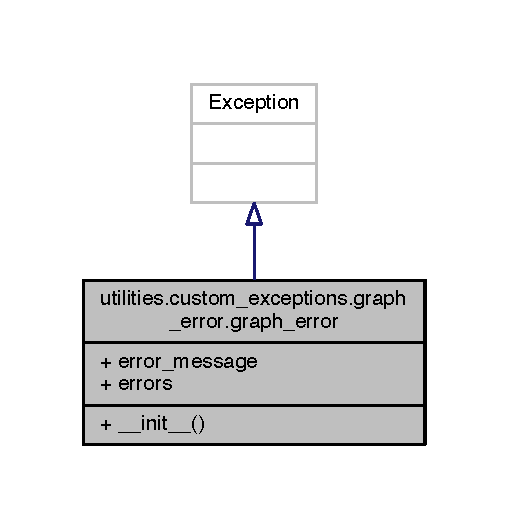
\includegraphics[width=244pt]{d4/d9a/classutilities_1_1custom__exceptions_1_1graph__error_1_1graph__error__inherit__graph}
\end{center}
\end{figure}


Collaboration diagram for utilities.\+custom\+\_\+exceptions.\+graph\+\_\+error.\+graph\+\_\+error\+:
\nopagebreak
\begin{figure}[H]
\begin{center}
\leavevmode
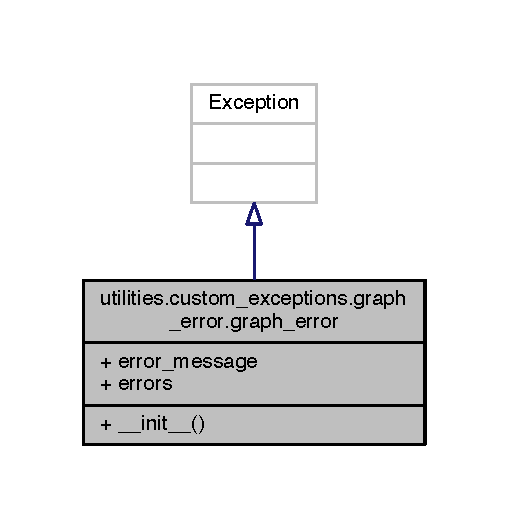
\includegraphics[width=244pt]{d6/d8d/classutilities_1_1custom__exceptions_1_1graph__error_1_1graph__error__coll__graph}
\end{center}
\end{figure}
\subsection*{Public Member Functions}
\begin{DoxyCompactItemize}
\item 
def \hyperlink{classutilities_1_1custom__exceptions_1_1graph__error_1_1graph__error_af1cd1f51b69ad2fc3af0521ae2922535}{\+\_\+\+\_\+init\+\_\+\+\_\+}
\begin{DoxyCompactList}\small\item\em Standard constructor for the graph\+\_\+exception class. \end{DoxyCompactList}\end{DoxyCompactItemize}
\subsection*{Public Attributes}
\begin{DoxyCompactItemize}
\item 
\hyperlink{classutilities_1_1custom__exceptions_1_1graph__error_1_1graph__error_a98eabd7ef4fec2794e8b88e3af478de6}{error\+\_\+message}
\item 
\hyperlink{classutilities_1_1custom__exceptions_1_1graph__error_1_1graph__error_abc34ad82ec3f8374e1ff60c5c888a3eb}{errors}
\end{DoxyCompactItemize}


\subsection{Detailed Description}
Import Custom Python Modules. 

Module of a custom graph\+\_\+exception that extends the default Python exception class. class my\+\_\+graph\+\_\+error(\+Exception)\+: 

Definition at line \hyperlink{graph__error_8py_source_l00085}{85} of file \hyperlink{graph__error_8py_source}{graph\+\_\+error.\+py}.



\subsection{Constructor \& Destructor Documentation}
\hypertarget{classutilities_1_1custom__exceptions_1_1graph__error_1_1graph__error_af1cd1f51b69ad2fc3af0521ae2922535}{}\index{utilities\+::custom\+\_\+exceptions\+::graph\+\_\+error\+::graph\+\_\+error@{utilities\+::custom\+\_\+exceptions\+::graph\+\_\+error\+::graph\+\_\+error}!\+\_\+\+\_\+init\+\_\+\+\_\+@{\+\_\+\+\_\+init\+\_\+\+\_\+}}
\index{\+\_\+\+\_\+init\+\_\+\+\_\+@{\+\_\+\+\_\+init\+\_\+\+\_\+}!utilities\+::custom\+\_\+exceptions\+::graph\+\_\+error\+::graph\+\_\+error@{utilities\+::custom\+\_\+exceptions\+::graph\+\_\+error\+::graph\+\_\+error}}
\subsubsection[{\+\_\+\+\_\+init\+\_\+\+\_\+}]{\setlength{\rightskip}{0pt plus 5cm}def utilities.\+custom\+\_\+exceptions.\+graph\+\_\+error.\+graph\+\_\+error.\+\_\+\+\_\+init\+\_\+\+\_\+ (
\begin{DoxyParamCaption}
\item[{}]{self, }
\item[{}]{error\+\_\+message, }
\item[{}]{errors = {\ttfamily None}}
\end{DoxyParamCaption}
)}\label{classutilities_1_1custom__exceptions_1_1graph__error_1_1graph__error_af1cd1f51b69ad2fc3af0521ae2922535}


Standard constructor for the graph\+\_\+exception class. 


\begin{DoxyParams}{Parameters}
{\em self} & -\/ This instance of the graph\+\_\+exception class. \\
\hline
{\em error\+\_\+message} & -\/ Custom error message included when raising/throwing this graph\+\_\+exception class. \\
\hline
{\em errors} & -\/ Associted errors to this instance of the graph\+\_\+exception. \\
\hline
\end{DoxyParams}


Definition at line \hyperlink{graph__error_8py_source_l00092}{92} of file \hyperlink{graph__error_8py_source}{graph\+\_\+error.\+py}.


\begin{DoxyCode}
\hypertarget{classutilities_1_1custom__exceptions_1_1graph__error_1_1graph__error_l00092}{}\hyperlink{classutilities_1_1custom__exceptions_1_1graph__error_1_1graph__error_af1cd1f51b69ad2fc3af0521ae2922535}{00092}     \textcolor{keyword}{def }\hyperlink{classutilities_1_1custom__exceptions_1_1graph__error_1_1graph__error_af1cd1f51b69ad2fc3af0521ae2922535}{\_\_init\_\_}(self, error\_message, errors=None):
\hypertarget{classutilities_1_1custom__exceptions_1_1graph__error_1_1graph__error_l00093}{}\hyperlink{classutilities_1_1custom__exceptions_1_1graph__error_1_1graph__error_a98eabd7ef4fec2794e8b88e3af478de6}{00093}         self.\hyperlink{classutilities_1_1custom__exceptions_1_1graph__error_1_1graph__error_a98eabd7ef4fec2794e8b88e3af478de6}{error\_message} = error\_message
00094         \textcolor{comment}{# Custom code: Assign associated errors.}
\hypertarget{classutilities_1_1custom__exceptions_1_1graph__error_1_1graph__error_l00095}{}\hyperlink{classutilities_1_1custom__exceptions_1_1graph__error_1_1graph__error_abc34ad82ec3f8374e1ff60c5c888a3eb}{00095}         self.\hyperlink{classutilities_1_1custom__exceptions_1_1graph__error_1_1graph__error_abc34ad82ec3f8374e1ff60c5c888a3eb}{errors} = errors
00096         \textcolor{comment}{# Call base class, Exception, constructor with required}
00097         \textcolor{comment}{#   parameters.}
00098         super(graph\_error, self).\hyperlink{classutilities_1_1custom__exceptions_1_1graph__error_1_1graph__error_af1cd1f51b69ad2fc3af0521ae2922535}{\_\_init\_\_}(\textcolor{stringliteral}{'error message: \{\}, list of errors: \{\}'}.format(
      error\_message, errors))
00099         \textcolor{comment}{#super(graph\_error, self).\_\_init\_\_(error\_message)}
00100         \textcolor{comment}{# Override the "\_\_reduce\_\_" method.}
00101         \textcolor{keyword}{def }\_\_reduce\_\_(self):
00102             \textcolor{keywordflow}{return} (graph\_error, (self.arg1, self.arg2))
00103 \end{DoxyCode}


\subsection{Member Data Documentation}
\hypertarget{classutilities_1_1custom__exceptions_1_1graph__error_1_1graph__error_a98eabd7ef4fec2794e8b88e3af478de6}{}\index{utilities\+::custom\+\_\+exceptions\+::graph\+\_\+error\+::graph\+\_\+error@{utilities\+::custom\+\_\+exceptions\+::graph\+\_\+error\+::graph\+\_\+error}!error\+\_\+message@{error\+\_\+message}}
\index{error\+\_\+message@{error\+\_\+message}!utilities\+::custom\+\_\+exceptions\+::graph\+\_\+error\+::graph\+\_\+error@{utilities\+::custom\+\_\+exceptions\+::graph\+\_\+error\+::graph\+\_\+error}}
\subsubsection[{error\+\_\+message}]{\setlength{\rightskip}{0pt plus 5cm}utilities.\+custom\+\_\+exceptions.\+graph\+\_\+error.\+graph\+\_\+error.\+error\+\_\+message}\label{classutilities_1_1custom__exceptions_1_1graph__error_1_1graph__error_a98eabd7ef4fec2794e8b88e3af478de6}


Definition at line \hyperlink{graph__error_8py_source_l00093}{93} of file \hyperlink{graph__error_8py_source}{graph\+\_\+error.\+py}.

\hypertarget{classutilities_1_1custom__exceptions_1_1graph__error_1_1graph__error_abc34ad82ec3f8374e1ff60c5c888a3eb}{}\index{utilities\+::custom\+\_\+exceptions\+::graph\+\_\+error\+::graph\+\_\+error@{utilities\+::custom\+\_\+exceptions\+::graph\+\_\+error\+::graph\+\_\+error}!errors@{errors}}
\index{errors@{errors}!utilities\+::custom\+\_\+exceptions\+::graph\+\_\+error\+::graph\+\_\+error@{utilities\+::custom\+\_\+exceptions\+::graph\+\_\+error\+::graph\+\_\+error}}
\subsubsection[{errors}]{\setlength{\rightskip}{0pt plus 5cm}utilities.\+custom\+\_\+exceptions.\+graph\+\_\+error.\+graph\+\_\+error.\+errors}\label{classutilities_1_1custom__exceptions_1_1graph__error_1_1graph__error_abc34ad82ec3f8374e1ff60c5c888a3eb}


Definition at line \hyperlink{graph__error_8py_source_l00095}{95} of file \hyperlink{graph__error_8py_source}{graph\+\_\+error.\+py}.



The documentation for this class was generated from the following file\+:\begin{DoxyCompactItemize}
\item 
utilities/custom\+\_\+exceptions/\hyperlink{graph__error_8py}{graph\+\_\+error.\+py}\end{DoxyCompactItemize}

\hypertarget{classutilities_1_1custom__exceptions_1_1graph__error__tester_1_1graph__error__tester}{}\section{utilities.\+custom\+\_\+exceptions.\+graph\+\_\+error\+\_\+tester.\+graph\+\_\+error\+\_\+tester Class Reference}
\label{classutilities_1_1custom__exceptions_1_1graph__error__tester_1_1graph__error__tester}\index{utilities.\+custom\+\_\+exceptions.\+graph\+\_\+error\+\_\+tester.\+graph\+\_\+error\+\_\+tester@{utilities.\+custom\+\_\+exceptions.\+graph\+\_\+error\+\_\+tester.\+graph\+\_\+error\+\_\+tester}}


Collaboration diagram for utilities.\+custom\+\_\+exceptions.\+graph\+\_\+error\+\_\+tester.\+graph\+\_\+error\+\_\+tester\+:
\nopagebreak
\begin{figure}[H]
\begin{center}
\leavevmode
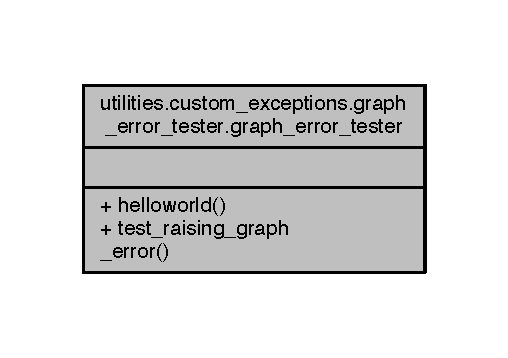
\includegraphics[width=244pt]{d9/d84/classutilities_1_1custom__exceptions_1_1graph__error__tester_1_1graph__error__tester__coll__graph}
\end{center}
\end{figure}
\subsection*{Static Public Member Functions}
\begin{DoxyCompactItemize}
\item 
def \hyperlink{classutilities_1_1custom__exceptions_1_1graph__error__tester_1_1graph__error__tester_a59e456a82b205066fe96b206ba70411f}{helloworld} ()
\begin{DoxyCompactList}\small\item\em ========================================================= Method to test throwing/raising the \hyperlink{namespaceutilities_1_1custom__exceptions_1_1graph__error}{graph\+\_\+error} exception. \end{DoxyCompactList}\item 
def \hyperlink{classutilities_1_1custom__exceptions_1_1graph__error__tester_1_1graph__error__tester_a844b0064bc87b5d840f5cf3f54d99240}{test\+\_\+raising\+\_\+graph\+\_\+error} ()
\begin{DoxyCompactList}\small\item\em ========================================================= Method to test throwing/raising the \hyperlink{namespaceutilities_1_1custom__exceptions_1_1graph__error}{graph\+\_\+error} exception. \end{DoxyCompactList}\end{DoxyCompactItemize}


\subsection{Detailed Description}


Definition at line \hyperlink{graph__error__tester_8py_source_l00093}{93} of file \hyperlink{graph__error__tester_8py_source}{graph\+\_\+error\+\_\+tester.\+py}.



\subsection{Member Function Documentation}
\hypertarget{classutilities_1_1custom__exceptions_1_1graph__error__tester_1_1graph__error__tester_a59e456a82b205066fe96b206ba70411f}{}\index{utilities\+::custom\+\_\+exceptions\+::graph\+\_\+error\+\_\+tester\+::graph\+\_\+error\+\_\+tester@{utilities\+::custom\+\_\+exceptions\+::graph\+\_\+error\+\_\+tester\+::graph\+\_\+error\+\_\+tester}!helloworld@{helloworld}}
\index{helloworld@{helloworld}!utilities\+::custom\+\_\+exceptions\+::graph\+\_\+error\+\_\+tester\+::graph\+\_\+error\+\_\+tester@{utilities\+::custom\+\_\+exceptions\+::graph\+\_\+error\+\_\+tester\+::graph\+\_\+error\+\_\+tester}}
\subsubsection[{helloworld()}]{\setlength{\rightskip}{0pt plus 5cm}def utilities.\+custom\+\_\+exceptions.\+graph\+\_\+error\+\_\+tester.\+graph\+\_\+error\+\_\+tester.\+helloworld (
\begin{DoxyParamCaption}
{}
\end{DoxyParamCaption}
)\hspace{0.3cm}{\ttfamily [static]}}\label{classutilities_1_1custom__exceptions_1_1graph__error__tester_1_1graph__error__tester_a59e456a82b205066fe96b206ba70411f}


========================================================= Method to test throwing/raising the \hyperlink{namespaceutilities_1_1custom__exceptions_1_1graph__error}{graph\+\_\+error} exception. 


\begin{DoxyParams}{Parameters}
{\em -\/} & Nothing \\
\hline
\end{DoxyParams}
\begin{DoxyReturn}{Returns}
-\/ Nothing. O(1) method. 
\end{DoxyReturn}


Definition at line \hyperlink{graph__error__tester_8py_source_l00100}{100} of file \hyperlink{graph__error__tester_8py_source}{graph\+\_\+error\+\_\+tester.\+py}.


\begin{DoxyCode}
\hypertarget{classutilities_1_1custom__exceptions_1_1graph__error__tester_1_1graph__error__tester_l00100}{}\hyperlink{classutilities_1_1custom__exceptions_1_1graph__error__tester_1_1graph__error__tester_a59e456a82b205066fe96b206ba70411f}{00100}     \textcolor{keyword}{def }\hyperlink{classutilities_1_1custom__exceptions_1_1graph__error__tester_1_1graph__error__tester_a59e456a82b205066fe96b206ba70411f}{helloworld}():
00101         print(\textcolor{stringliteral}{":::  graph\_error accessor method works."})
\end{DoxyCode}
\hypertarget{classutilities_1_1custom__exceptions_1_1graph__error__tester_1_1graph__error__tester_a844b0064bc87b5d840f5cf3f54d99240}{}\index{utilities\+::custom\+\_\+exceptions\+::graph\+\_\+error\+\_\+tester\+::graph\+\_\+error\+\_\+tester@{utilities\+::custom\+\_\+exceptions\+::graph\+\_\+error\+\_\+tester\+::graph\+\_\+error\+\_\+tester}!test\+\_\+raising\+\_\+graph\+\_\+error@{test\+\_\+raising\+\_\+graph\+\_\+error}}
\index{test\+\_\+raising\+\_\+graph\+\_\+error@{test\+\_\+raising\+\_\+graph\+\_\+error}!utilities\+::custom\+\_\+exceptions\+::graph\+\_\+error\+\_\+tester\+::graph\+\_\+error\+\_\+tester@{utilities\+::custom\+\_\+exceptions\+::graph\+\_\+error\+\_\+tester\+::graph\+\_\+error\+\_\+tester}}
\subsubsection[{test\+\_\+raising\+\_\+graph\+\_\+error()}]{\setlength{\rightskip}{0pt plus 5cm}def utilities.\+custom\+\_\+exceptions.\+graph\+\_\+error\+\_\+tester.\+graph\+\_\+error\+\_\+tester.\+test\+\_\+raising\+\_\+graph\+\_\+error (
\begin{DoxyParamCaption}
{}
\end{DoxyParamCaption}
)\hspace{0.3cm}{\ttfamily [static]}}\label{classutilities_1_1custom__exceptions_1_1graph__error__tester_1_1graph__error__tester_a844b0064bc87b5d840f5cf3f54d99240}


========================================================= Method to test throwing/raising the \hyperlink{namespaceutilities_1_1custom__exceptions_1_1graph__error}{graph\+\_\+error} exception. 


\begin{DoxyParams}{Parameters}
{\em -\/} & Nothing \\
\hline
\end{DoxyParams}
\begin{DoxyReturn}{Returns}
-\/ Nothing. O(1) method. 
\end{DoxyReturn}


Definition at line \hyperlink{graph__error__tester_8py_source_l00108}{108} of file \hyperlink{graph__error__tester_8py_source}{graph\+\_\+error\+\_\+tester.\+py}.


\begin{DoxyCode}
\hypertarget{classutilities_1_1custom__exceptions_1_1graph__error__tester_1_1graph__error__tester_l00108}{}\hyperlink{classutilities_1_1custom__exceptions_1_1graph__error__tester_1_1graph__error__tester_a844b0064bc87b5d840f5cf3f54d99240}{00108}     \textcolor{keyword}{def }\hyperlink{classutilities_1_1custom__exceptions_1_1graph__error__tester_1_1graph__error__tester_a844b0064bc87b5d840f5cf3f54d99240}{test\_raising\_graph\_error}():
00109         print(\textcolor{stringliteral}{""})
00110         print(\textcolor{stringliteral}{"==   Testing the graph\_error class/module."})
00111         \textcolor{keywordflow}{try}:
00112             prompt = \textcolor{stringliteral}{"  ... Test: raise graph\_error exception, 2 arguments  \{\}"}
00113             statistical\_analysis.increment\_number\_test\_cases\_used()
00114             \textcolor{comment}{#raise graph\_error("Can graph\_error be caught")}
00115             \textcolor{comment}{#raise utilities.custom\_exceptions.graph\_error("Can graph\_error be caught")}
00116             \textcolor{keywordflow}{raise} \hyperlink{classutilities_1_1custom__exceptions_1_1graph__error_1_1graph__error}{graph\_error}(\textcolor{stringliteral}{"Can graph\_error be caught?"},\textcolor{stringliteral}{"gyou"})
00117         \textcolor{comment}{#except utilities.custom\_exceptions.graph\_error:}
00118         \textcolor{keywordflow}{except} graph\_error:
00119             print(prompt .format(\textcolor{stringliteral}{"OK"}))
00120             statistical\_analysis.increment\_number\_test\_cases\_passed()
00121         \textcolor{keywordflow}{else}:
00122             print(prompt .format(\textcolor{stringliteral}{"FAIL!!!"}))
00123         \textcolor{keywordflow}{try}:
00124             prompt = \textcolor{stringliteral}{"  ... Test: raise graph\_error exception, 1 argument   \{\}"}
00125             statistical\_analysis.increment\_number\_test\_cases\_used()
00126             \textcolor{comment}{#raise graph\_error("Can graph\_error be caught")}
00127             \textcolor{comment}{#raise utilities.custom\_exceptions.graph\_error("Can graph\_error be caught")}
00128             \textcolor{keywordflow}{raise} \hyperlink{classutilities_1_1custom__exceptions_1_1graph__error_1_1graph__error}{graph\_error}(\textcolor{stringliteral}{"Can graph\_error be caught?"})
00129         \textcolor{comment}{#except utilities.custom\_exceptions.graph\_error:}
00130         \textcolor{keywordflow}{except} graph\_error:
00131             print(prompt .format(\textcolor{stringliteral}{"OK"}))
00132             statistical\_analysis.increment\_number\_test\_cases\_passed()
00133         \textcolor{keywordflow}{else}:
00134             print(prompt .format(\textcolor{stringliteral}{"FAIL!!!"}))
00135 \end{DoxyCode}


The documentation for this class was generated from the following file\+:\begin{DoxyCompactItemize}
\item 
utilities/custom\+\_\+exceptions/\hyperlink{graph__error__tester_8py}{graph\+\_\+error\+\_\+tester.\+py}\end{DoxyCompactItemize}

\hypertarget{classincremental__test_1_1incremental__test__automation}{}\section{incremental\+\_\+test.\+incremental\+\_\+test\+\_\+automation Class Reference}
\label{classincremental__test_1_1incremental__test__automation}\index{incremental\+\_\+test.\+incremental\+\_\+test\+\_\+automation@{incremental\+\_\+test.\+incremental\+\_\+test\+\_\+automation}}


Collaboration diagram for incremental\+\_\+test.\+incremental\+\_\+test\+\_\+automation\+:
\nopagebreak
\begin{figure}[H]
\begin{center}
\leavevmode

\includegraphics[width=224pt]{dc/d3c/classincremental__test_1_1incremental__test__automation__coll__graph}
\end{center}
\end{figure}
\subsection*{Static Public Attributes}
\begin{DoxyCompactItemize}
\item 
string \hyperlink{classincremental__test_1_1incremental__test__automation_afbbdcc0177de0d7d04bbf38ea90e9a5a}{result\+\_\+repository} = \char`\"{}$\sim$/Documents/ricerca/risultati\+\_\+sperimentali/std-\/cell-\/library-\/characterization\char`\"{}
\end{DoxyCompactItemize}


\subsection{Detailed Description}


Definition at line \hyperlink{incremental__test_8py_source_l00160}{160} of file \hyperlink{incremental__test_8py_source}{incremental\+\_\+test.\+py}.



\subsection{Member Data Documentation}
\hypertarget{classincremental__test_1_1incremental__test__automation_afbbdcc0177de0d7d04bbf38ea90e9a5a}{}\index{incremental\+\_\+test\+::incremental\+\_\+test\+\_\+automation@{incremental\+\_\+test\+::incremental\+\_\+test\+\_\+automation}!result\+\_\+repository@{result\+\_\+repository}}
\index{result\+\_\+repository@{result\+\_\+repository}!incremental\+\_\+test\+::incremental\+\_\+test\+\_\+automation@{incremental\+\_\+test\+::incremental\+\_\+test\+\_\+automation}}
\subsubsection[{result\+\_\+repository}]{\setlength{\rightskip}{0pt plus 5cm}string incremental\+\_\+test.\+incremental\+\_\+test\+\_\+automation.\+result\+\_\+repository = \char`\"{}$\sim$/Documents/ricerca/risultati\+\_\+sperimentali/std-\/cell-\/library-\/characterization\char`\"{}\hspace{0.3cm}{\ttfamily [static]}}\label{classincremental__test_1_1incremental__test__automation_afbbdcc0177de0d7d04bbf38ea90e9a5a}


Definition at line \hyperlink{incremental__test_8py_source_l00163}{163} of file \hyperlink{incremental__test_8py_source}{incremental\+\_\+test.\+py}.



The documentation for this class was generated from the following file\+:\begin{DoxyCompactItemize}
\item 
\hyperlink{incremental__test_8py}{incremental\+\_\+test.\+py}\end{DoxyCompactItemize}

\hypertarget{classutilities_1_1miscellaneous_1_1misc}{}\section{utilities.\+miscellaneous.\+misc Class Reference}
\label{classutilities_1_1miscellaneous_1_1misc}\index{utilities.\+miscellaneous.\+misc@{utilities.\+miscellaneous.\+misc}}


Module with methods that perform miscellaneous tasks.  




Collaboration diagram for utilities.\+miscellaneous.\+misc\+:
\nopagebreak
\begin{figure}[H]
\begin{center}
\leavevmode

\includegraphics[width=228pt]{d9/d28/classutilities_1_1miscellaneous_1_1misc__coll__graph}
\end{center}
\end{figure}
\subsection*{Static Public Member Functions}
\begin{DoxyCompactItemize}
\item 
def \hyperlink{classutilities_1_1miscellaneous_1_1misc_a17714d8ce76a7c4f04256b37b9938c15}{get\+\_\+absolute\+\_\+path\+\_\+to\+\_\+store\+\_\+results} ()
\begin{DoxyCompactList}\small\item\em Method to get the absolute path to store results. \end{DoxyCompactList}\item 
def \hyperlink{classutilities_1_1miscellaneous_1_1misc_a9b5ff2b3036d8a1a2e3bacb1d25e2785}{check\+\_\+absolute\+\_\+path\+\_\+to\+\_\+store\+\_\+results} (path\+\_\+to\+\_\+file, filename)
\begin{DoxyCompactList}\small\item\em Method to validate the absolute path to store results. \end{DoxyCompactList}\item 
def \hyperlink{classutilities_1_1miscellaneous_1_1misc_a96b7b4aa054c6c8eb7571314ec8edbc7}{check\+\_\+filename\+\_\+format} (filename)
\begin{DoxyCompactList}\small\item\em Method to determine if a filename has the D\+D-\/\+M\+M-\/\+Y\+Y-\/\+H\+H-\/\+M\+M-\/\+S\+S-\/u\+S.\+txt format. \end{DoxyCompactList}\item 
def \hyperlink{classutilities_1_1miscellaneous_1_1misc_ab675e34a1a463f5a6aac272debe372ae}{find\+\_\+desired\+\_\+location\+\_\+for\+\_\+results} (filename)
\begin{DoxyCompactList}\small\item\em Method to determine where to store the results of the experimental, simulation, verification, or testing runs. \end{DoxyCompactList}\item 
def \hyperlink{classutilities_1_1miscellaneous_1_1misc_ad364ae88435c58955e26fcc22b1cabb9}{store\+\_\+results} (path\+\_\+to\+\_\+file)
\begin{DoxyCompactList}\small\item\em Method to store the results file in the specified absolute path. \end{DoxyCompactList}\item 
def \hyperlink{classutilities_1_1miscellaneous_1_1misc_a7837597eba06ec38b69b931ec18e39eb}{add\+\_\+commit\+\_\+push\+\_\+updates\+\_\+to\+\_\+git\+\_\+repository} (comment)
\begin{DoxyCompactList}\small\item\em Method to add, commit, and push additions and updates to a Git repository. \end{DoxyCompactList}\end{DoxyCompactItemize}
\subsection*{Static Public Attributes}
\begin{DoxyCompactItemize}
\item 
string \hyperlink{classutilities_1_1miscellaneous_1_1misc_a27fd16369fd0995d7494ff4741de5b91}{absolute\+\_\+path\+\_\+to\+\_\+store\+\_\+results} = \char`\"{}/Users/zhiyang/Documents/ricerca/risultati\+\_\+sperimentali/std-\/cell-\/library-\/characterization\char`\"{}
\end{DoxyCompactItemize}


\subsection{Detailed Description}
Module with methods that perform miscellaneous tasks. 



Definition at line \hyperlink{miscellaneous_8py_source_l00095}{95} of file \hyperlink{miscellaneous_8py_source}{miscellaneous.\+py}.



\subsection{Member Function Documentation}
\hypertarget{classutilities_1_1miscellaneous_1_1misc_a7837597eba06ec38b69b931ec18e39eb}{}\index{utilities\+::miscellaneous\+::misc@{utilities\+::miscellaneous\+::misc}!add\+\_\+commit\+\_\+push\+\_\+updates\+\_\+to\+\_\+git\+\_\+repository@{add\+\_\+commit\+\_\+push\+\_\+updates\+\_\+to\+\_\+git\+\_\+repository}}
\index{add\+\_\+commit\+\_\+push\+\_\+updates\+\_\+to\+\_\+git\+\_\+repository@{add\+\_\+commit\+\_\+push\+\_\+updates\+\_\+to\+\_\+git\+\_\+repository}!utilities\+::miscellaneous\+::misc@{utilities\+::miscellaneous\+::misc}}
\subsubsection[{add\+\_\+commit\+\_\+push\+\_\+updates\+\_\+to\+\_\+git\+\_\+repository(comment)}]{\setlength{\rightskip}{0pt plus 5cm}def utilities.\+miscellaneous.\+misc.\+add\+\_\+commit\+\_\+push\+\_\+updates\+\_\+to\+\_\+git\+\_\+repository (
\begin{DoxyParamCaption}
\item[{}]{comment}
\end{DoxyParamCaption}
)\hspace{0.3cm}{\ttfamily [static]}}\label{classutilities_1_1miscellaneous_1_1misc_a7837597eba06ec38b69b931ec18e39eb}


Method to add, commit, and push additions and updates to a Git repository. 


\begin{DoxyParams}{Parameters}
{\em comment} & -\/ A comment for this commit/build \mbox{[}to the repository\mbox{]}. \\
\hline
\end{DoxyParams}
\begin{DoxyReturn}{Returns}
boolean True if updates can be added, committed, and push additions to a Git repository; Else, return boolean False. O(1) method. 
\end{DoxyReturn}


Definition at line \hyperlink{miscellaneous_8py_source_l00235}{235} of file \hyperlink{miscellaneous_8py_source}{miscellaneous.\+py}.


\begin{DoxyCode}
\hypertarget{classutilities_1_1miscellaneous_1_1misc_l00235}{}\hyperlink{classutilities_1_1miscellaneous_1_1misc_a7837597eba06ec38b69b931ec18e39eb}{00235}     \textcolor{keyword}{def }\hyperlink{classutilities_1_1miscellaneous_1_1misc_a7837597eba06ec38b69b931ec18e39eb}{add\_commit\_push\_updates\_to\_git\_repository}(comment):
00236         \textcolor{keywordflow}{try}:
00237             print(\textcolor{stringliteral}{"-------------------------------------------------"})
00238             cmd = [\textcolor{stringliteral}{'git'}, \textcolor{stringliteral}{'add'}, \textcolor{stringliteral}{"-A"}]
00239             p = subprocess.Popen(cmd, cwd=config\_manager.result\_repository)
00240             \textcolor{comment}{#p = subprocess.call(cmd, cwd=config\_manager.result\_repository)}
00241             print(\textcolor{stringliteral}{"-    Added. Commit now."})
00242             comment = \textcolor{stringliteral}{"Update build via Python."}
00243             cmd = [\textcolor{stringliteral}{"git"}, \textcolor{stringliteral}{"commit"}, \textcolor{stringliteral}{"-m"}, comment]
00244             p = subprocess.Popen(cmd, cwd=config\_manager.result\_repository)
00245             p.wait()
00246             print(\textcolor{stringliteral}{"-    Committed. Push now."})
00247             cmd = [\textcolor{stringliteral}{"git"}, \textcolor{stringliteral}{"push"}]
00248             p = subprocess.Popen(cmd, cwd=config\_manager.result\_repository)
00249             p.wait()
00250             print(\textcolor{stringliteral}{"-------------------------------------------------"})
00251             \textcolor{keywordflow}{return} \textcolor{keyword}{True}
00252         \textcolor{keywordflow}{except}:
00253             \textcolor{keywordflow}{return} \textcolor{keyword}{False}
00254 \end{DoxyCode}
\hypertarget{classutilities_1_1miscellaneous_1_1misc_a9b5ff2b3036d8a1a2e3bacb1d25e2785}{}\index{utilities\+::miscellaneous\+::misc@{utilities\+::miscellaneous\+::misc}!check\+\_\+absolute\+\_\+path\+\_\+to\+\_\+store\+\_\+results@{check\+\_\+absolute\+\_\+path\+\_\+to\+\_\+store\+\_\+results}}
\index{check\+\_\+absolute\+\_\+path\+\_\+to\+\_\+store\+\_\+results@{check\+\_\+absolute\+\_\+path\+\_\+to\+\_\+store\+\_\+results}!utilities\+::miscellaneous\+::misc@{utilities\+::miscellaneous\+::misc}}
\subsubsection[{check\+\_\+absolute\+\_\+path\+\_\+to\+\_\+store\+\_\+results(path\+\_\+to\+\_\+file, filename)}]{\setlength{\rightskip}{0pt plus 5cm}def utilities.\+miscellaneous.\+misc.\+check\+\_\+absolute\+\_\+path\+\_\+to\+\_\+store\+\_\+results (
\begin{DoxyParamCaption}
\item[{}]{path\+\_\+to\+\_\+file, }
\item[{}]{filename}
\end{DoxyParamCaption}
)\hspace{0.3cm}{\ttfamily [static]}}\label{classutilities_1_1miscellaneous_1_1misc_a9b5ff2b3036d8a1a2e3bacb1d25e2785}


Method to validate the absolute path to store results. 

It is an query method 
\begin{DoxyParams}{Parameters}
{\em path\+\_\+to\+\_\+file} & -\/ A path to store the results file. \\
\hline
{\em filename} & -\/ A filename. \\
\hline
\end{DoxyParams}
\begin{DoxyReturn}{Returns}
boolean True, if the path to the desired location can be contains the value in \char`\"{}misc.\+absolute\+\_\+path\+\_\+to\+\_\+store\+\_\+results\char`\"{} and the filename of the results file. Else, return boolean False. O(1) method. 
\end{DoxyReturn}


Definition at line \hyperlink{miscellaneous_8py_source_l00117}{117} of file \hyperlink{miscellaneous_8py_source}{miscellaneous.\+py}.


\begin{DoxyCode}
\hypertarget{classutilities_1_1miscellaneous_1_1misc_l00117}{}\hyperlink{classutilities_1_1miscellaneous_1_1misc_a9b5ff2b3036d8a1a2e3bacb1d25e2785}{00117}     \textcolor{keyword}{def }\hyperlink{classutilities_1_1miscellaneous_1_1misc_a9b5ff2b3036d8a1a2e3bacb1d25e2785}{check\_absolute\_path\_to\_store\_results}(path\_to\_file,filename):
00118         \textcolor{keywordflow}{if} path\_to\_file.find(filename):
00119             \textcolor{keywordflow}{return} \textcolor{keyword}{True}
00120         \textcolor{keywordflow}{else}:
00121             \textcolor{keywordflow}{return} \textcolor{keyword}{False}
\end{DoxyCode}
\hypertarget{classutilities_1_1miscellaneous_1_1misc_a96b7b4aa054c6c8eb7571314ec8edbc7}{}\index{utilities\+::miscellaneous\+::misc@{utilities\+::miscellaneous\+::misc}!check\+\_\+filename\+\_\+format@{check\+\_\+filename\+\_\+format}}
\index{check\+\_\+filename\+\_\+format@{check\+\_\+filename\+\_\+format}!utilities\+::miscellaneous\+::misc@{utilities\+::miscellaneous\+::misc}}
\subsubsection[{check\+\_\+filename\+\_\+format(filename)}]{\setlength{\rightskip}{0pt plus 5cm}def utilities.\+miscellaneous.\+misc.\+check\+\_\+filename\+\_\+format (
\begin{DoxyParamCaption}
\item[{}]{filename}
\end{DoxyParamCaption}
)\hspace{0.3cm}{\ttfamily [static]}}\label{classutilities_1_1miscellaneous_1_1misc_a96b7b4aa054c6c8eb7571314ec8edbc7}


Method to determine if a filename has the D\+D-\/\+M\+M-\/\+Y\+Y-\/\+H\+H-\/\+M\+M-\/\+S\+S-\/u\+S.\+txt format. 


\begin{DoxyParams}{Parameters}
{\em filename} & -\/ A filename. \\
\hline
\end{DoxyParams}
\begin{DoxyReturn}{Returns}
boolean True if the path to the desired location can be found; Else, return boolean False. O(1) method. 
\end{DoxyReturn}


Definition at line \hyperlink{miscellaneous_8py_source_l00131}{131} of file \hyperlink{miscellaneous_8py_source}{miscellaneous.\+py}.


\begin{DoxyCode}
\hypertarget{classutilities_1_1miscellaneous_1_1misc_l00131}{}\hyperlink{classutilities_1_1miscellaneous_1_1misc_a96b7b4aa054c6c8eb7571314ec8edbc7}{00131}     \textcolor{keyword}{def }\hyperlink{classutilities_1_1miscellaneous_1_1misc_a96b7b4aa054c6c8eb7571314ec8edbc7}{check\_filename\_format}(filename):
00132         filename\_wo\_extn, file\_extn = os.path.splitext(filename)
00133         \textcolor{keywordflow}{if} \textcolor{stringliteral}{".txt"} != file\_extn:
00134             \textcolor{keywordflow}{return} \textcolor{keyword}{False}
00135         tokens = filename\_wo\_extn.split(\textcolor{stringliteral}{"-"})
00136         \textcolor{stringliteral}{"""}
00137 \textcolor{stringliteral}{            Check against the format: DD-MM-YY-HH-MM-SS-uS[.txt].}
00138 \textcolor{stringliteral}{            tokens[0] = DD/Day}
00139 \textcolor{stringliteral}{            tokens[1] = MM/Month}
00140 \textcolor{stringliteral}{            tokens[2] = YY/Year}
00141 \textcolor{stringliteral}{            tokens[3] = HH/Hour}
00142 \textcolor{stringliteral}{            tokens[4] = MM/Minute}
00143 \textcolor{stringliteral}{            tokens[5] = [SS/Second]}
00144 \textcolor{stringliteral}{            tokens[6] = [uS/Microsecond]}
00145 \textcolor{stringliteral}{        """}
00146         \textcolor{keywordflow}{if} 7 != len(tokens):
00147             \textcolor{keywordflow}{return} \textcolor{keyword}{False}
00148         \textcolor{keywordflow}{if} 1 > int(tokens[0]):
00149             \textcolor{keywordflow}{return} \textcolor{keyword}{False}
00150         \textcolor{keywordflow}{if} 2 == int(tokens[1]) \textcolor{keywordflow}{and} 29 < int(tokens[0]) \textcolor{keywordflow}{and} calendar.isleap(int(tokens[2])):
00151             \textcolor{keywordflow}{return} \textcolor{keyword}{False}
00152         \textcolor{keywordflow}{if} 2 == int(tokens[1]) \textcolor{keywordflow}{and} 28 < int(tokens[0]) \textcolor{keywordflow}{and} \textcolor{keywordflow}{not} calendar.isleap(int(tokens[2])):
00153             \textcolor{keywordflow}{return} \textcolor{keyword}{False}
00154         \textcolor{keywordflow}{if} generate\_filename\_tester.is\_30\_day\_month(tokens[1]) \textcolor{keywordflow}{and} 30 < int(tokens[0]):
00155             \textcolor{keywordflow}{return} \textcolor{keyword}{False}
00156         \textcolor{keywordflow}{if} generate\_filename\_tester.is\_31\_day\_month(tokens[1]) \textcolor{keywordflow}{and} 31 < int(tokens[0]):
00157             \textcolor{keywordflow}{return} \textcolor{keyword}{False}
00158         \textcolor{keywordflow}{if} 1 > int(tokens[1]):
00159             \textcolor{keywordflow}{return} \textcolor{keyword}{False}
00160         \textcolor{keywordflow}{if} 12 < int(tokens[1]):
00161             \textcolor{keywordflow}{return} \textcolor{keyword}{False}
00162         \textcolor{keywordflow}{if} 2000 > int(tokens[2]):
00163             \textcolor{keywordflow}{return} \textcolor{keyword}{False}
00164         \textcolor{keywordflow}{if} 0 > int(tokens[3]):
00165             \textcolor{keywordflow}{return} \textcolor{keyword}{False}
00166         \textcolor{keywordflow}{if} 23 < int(tokens[3]):
00167             \textcolor{keywordflow}{return} \textcolor{keyword}{False}
00168         \textcolor{keywordflow}{if} 0 > int(tokens[4]):
00169             \textcolor{keywordflow}{return} \textcolor{keyword}{False}
00170         \textcolor{keywordflow}{if} 59 < int(tokens[4]):
00171             \textcolor{keywordflow}{return} \textcolor{keyword}{False}
00172         \textcolor{keywordflow}{if} 0 > int(tokens[5]):
00173             \textcolor{keywordflow}{return} \textcolor{keyword}{False}
00174         \textcolor{keywordflow}{if} 59 < int(tokens[5]):
00175             \textcolor{keywordflow}{return} \textcolor{keyword}{False}
00176         \textcolor{keywordflow}{if} 0 > int(tokens[6]):
00177             \textcolor{keywordflow}{return} \textcolor{keyword}{False}
00178         \textcolor{keywordflow}{if} 999999 < int(tokens[6]):
00179             \textcolor{keywordflow}{return} \textcolor{keyword}{False}
00180         \textcolor{keywordflow}{return} \textcolor{keyword}{True}
\end{DoxyCode}
\hypertarget{classutilities_1_1miscellaneous_1_1misc_ab675e34a1a463f5a6aac272debe372ae}{}\index{utilities\+::miscellaneous\+::misc@{utilities\+::miscellaneous\+::misc}!find\+\_\+desired\+\_\+location\+\_\+for\+\_\+results@{find\+\_\+desired\+\_\+location\+\_\+for\+\_\+results}}
\index{find\+\_\+desired\+\_\+location\+\_\+for\+\_\+results@{find\+\_\+desired\+\_\+location\+\_\+for\+\_\+results}!utilities\+::miscellaneous\+::misc@{utilities\+::miscellaneous\+::misc}}
\subsubsection[{find\+\_\+desired\+\_\+location\+\_\+for\+\_\+results(filename)}]{\setlength{\rightskip}{0pt plus 5cm}def utilities.\+miscellaneous.\+misc.\+find\+\_\+desired\+\_\+location\+\_\+for\+\_\+results (
\begin{DoxyParamCaption}
\item[{}]{filename}
\end{DoxyParamCaption}
)\hspace{0.3cm}{\ttfamily [static]}}\label{classutilities_1_1miscellaneous_1_1misc_ab675e34a1a463f5a6aac272debe372ae}


Method to determine where to store the results of the experimental, simulation, verification, or testing runs. 


\begin{DoxyParams}{Parameters}
{\em filename} & -\/ A filename that has the D\+D-\/\+M\+M-\/\+Y\+Y-\/\+H\+H-\/\+M\+M-\/\+S\+S-\/u\+S.\+txt. \\
\hline
\end{DoxyParams}
\begin{DoxyReturn}{Returns}
a string representing the absolute path of the location. O(1) method. 
\end{DoxyReturn}


Definition at line \hyperlink{miscellaneous_8py_source_l00188}{188} of file \hyperlink{miscellaneous_8py_source}{miscellaneous.\+py}.


\begin{DoxyCode}
\hypertarget{classutilities_1_1miscellaneous_1_1misc_l00188}{}\hyperlink{classutilities_1_1miscellaneous_1_1misc_ab675e34a1a463f5a6aac272debe372ae}{00188}     \textcolor{keyword}{def }\hyperlink{classutilities_1_1miscellaneous_1_1misc_ab675e34a1a463f5a6aac272debe372ae}{find\_desired\_location\_for\_results}(filename):
00189         \textcolor{comment}{# Does filename have the DD-MM-YY-HH-MM-SS-uS.txt format?}
00190         \textcolor{keywordflow}{if} \textcolor{keywordflow}{not} misc.check\_filename\_format(filename):
00191             \textcolor{keywordflow}{return} \textcolor{stringliteral}{"'filename' needs to have the format: DD-MM-YY-HH-MM-SS-uS.txt."}
00192         \textcolor{comment}{# Remove file extension, and tokenize the filename.}
00193         filename\_wo\_extn, file\_extn = os.path.splitext(filename)
00194         tokens = filename\_wo\_extn.split(\textcolor{stringliteral}{"-"})
00195         \textcolor{stringliteral}{"""}
00196 \textcolor{stringliteral}{            In the repository to store results from experiments,}
00197 \textcolor{stringliteral}{                simulations, and verification runs, and testing runs,}
00198 \textcolor{stringliteral}{                classify the files by subdirectories according to year}
00199 \textcolor{stringliteral}{                first before the month.}
00200 \textcolor{stringliteral}{        """}
00201         \textcolor{comment}{# Does a directory for the specified year exists?}
00202         path\_to\_results\_file = misc.get\_absolute\_path\_to\_store\_results() +  \textcolor{stringliteral}{"/"} + tokens[2]
00203         \textcolor{keywordflow}{if} \textcolor{keywordflow}{not} os.path.isdir(path\_to\_results\_file):
00204             \textcolor{comment}{# Creat the directory for the specified year.}
00205             os.mkdir(path\_to\_results\_file)
00206         \textcolor{comment}{# Does a directory for the specified month exists?}
00207         path\_to\_results\_file = path\_to\_results\_file + \textcolor{stringliteral}{"/"} + month\_name[int(tokens[1])].lower()
00208         \textcolor{keywordflow}{if} \textcolor{keywordflow}{not} os.path.isdir(path\_to\_results\_file):
00209             \textcolor{comment}{# Creat the directory for the specified month.}
00210             os.mkdir(path\_to\_results\_file)
00211         path\_to\_results\_file = path\_to\_results\_file + \textcolor{stringliteral}{"/"} + filename
00212         \textcolor{comment}{#print("path\_to\_results\_file:",path\_to\_results\_file,"=")}
00213         \textcolor{keywordflow}{return} path\_to\_results\_file
\end{DoxyCode}
\hypertarget{classutilities_1_1miscellaneous_1_1misc_a17714d8ce76a7c4f04256b37b9938c15}{}\index{utilities\+::miscellaneous\+::misc@{utilities\+::miscellaneous\+::misc}!get\+\_\+absolute\+\_\+path\+\_\+to\+\_\+store\+\_\+results@{get\+\_\+absolute\+\_\+path\+\_\+to\+\_\+store\+\_\+results}}
\index{get\+\_\+absolute\+\_\+path\+\_\+to\+\_\+store\+\_\+results@{get\+\_\+absolute\+\_\+path\+\_\+to\+\_\+store\+\_\+results}!utilities\+::miscellaneous\+::misc@{utilities\+::miscellaneous\+::misc}}
\subsubsection[{get\+\_\+absolute\+\_\+path\+\_\+to\+\_\+store\+\_\+results()}]{\setlength{\rightskip}{0pt plus 5cm}def utilities.\+miscellaneous.\+misc.\+get\+\_\+absolute\+\_\+path\+\_\+to\+\_\+store\+\_\+results (
\begin{DoxyParamCaption}
{}
\end{DoxyParamCaption}
)\hspace{0.3cm}{\ttfamily [static]}}\label{classutilities_1_1miscellaneous_1_1misc_a17714d8ce76a7c4f04256b37b9938c15}


Method to get the absolute path to store results. 

It is an accessor method. 
\begin{DoxyParams}{Parameters}
{\em -\/} & Nothing. \\
\hline
\end{DoxyParams}
\begin{DoxyReturn}{Returns}
the absolute path to store results. O(1) method. 
\end{DoxyReturn}


Definition at line \hyperlink{miscellaneous_8py_source_l00104}{104} of file \hyperlink{miscellaneous_8py_source}{miscellaneous.\+py}.


\begin{DoxyCode}
\hypertarget{classutilities_1_1miscellaneous_1_1misc_l00104}{}\hyperlink{classutilities_1_1miscellaneous_1_1misc_a17714d8ce76a7c4f04256b37b9938c15}{00104}     \textcolor{keyword}{def }\hyperlink{classutilities_1_1miscellaneous_1_1misc_a17714d8ce76a7c4f04256b37b9938c15}{get\_absolute\_path\_to\_store\_results}():
00105         \textcolor{keywordflow}{return} misc.absolute\_path\_to\_store\_results
\end{DoxyCode}
\hypertarget{classutilities_1_1miscellaneous_1_1misc_ad364ae88435c58955e26fcc22b1cabb9}{}\index{utilities\+::miscellaneous\+::misc@{utilities\+::miscellaneous\+::misc}!store\+\_\+results@{store\+\_\+results}}
\index{store\+\_\+results@{store\+\_\+results}!utilities\+::miscellaneous\+::misc@{utilities\+::miscellaneous\+::misc}}
\subsubsection[{store\+\_\+results(path\+\_\+to\+\_\+file)}]{\setlength{\rightskip}{0pt plus 5cm}def utilities.\+miscellaneous.\+misc.\+store\+\_\+results (
\begin{DoxyParamCaption}
\item[{}]{path\+\_\+to\+\_\+file}
\end{DoxyParamCaption}
)\hspace{0.3cm}{\ttfamily [static]}}\label{classutilities_1_1miscellaneous_1_1misc_ad364ae88435c58955e26fcc22b1cabb9}


Method to store the results file in the specified absolute path. 


\begin{DoxyParams}{Parameters}
{\em path\+\_\+to\+\_\+file} & -\/ A path to store the results file. \\
\hline
\end{DoxyParams}
\begin{DoxyReturn}{Returns}
a file object for the results file. O(1) method. 
\end{DoxyReturn}


Definition at line \hyperlink{miscellaneous_8py_source_l00220}{220} of file \hyperlink{miscellaneous_8py_source}{miscellaneous.\+py}.


\begin{DoxyCode}
\hypertarget{classutilities_1_1miscellaneous_1_1misc_l00220}{}\hyperlink{classutilities_1_1miscellaneous_1_1misc_ad364ae88435c58955e26fcc22b1cabb9}{00220}     \textcolor{keyword}{def }\hyperlink{classutilities_1_1miscellaneous_1_1misc_ad364ae88435c58955e26fcc22b1cabb9}{store\_results}(path\_to\_file):
00221         \textcolor{keywordflow}{if} path\_to\_file \textcolor{keywordflow}{is} \textcolor{keywordflow}{not} \textcolor{keywordtype}{None}:
00222             \textcolor{keywordflow}{return} open(path\_to\_file, \textcolor{stringliteral}{'w+'})
00223         \textcolor{keywordflow}{else}:
00224             \textcolor{keywordflow}{return} \textcolor{keywordtype}{None}
\end{DoxyCode}


\subsection{Member Data Documentation}
\hypertarget{classutilities_1_1miscellaneous_1_1misc_a27fd16369fd0995d7494ff4741de5b91}{}\index{utilities\+::miscellaneous\+::misc@{utilities\+::miscellaneous\+::misc}!absolute\+\_\+path\+\_\+to\+\_\+store\+\_\+results@{absolute\+\_\+path\+\_\+to\+\_\+store\+\_\+results}}
\index{absolute\+\_\+path\+\_\+to\+\_\+store\+\_\+results@{absolute\+\_\+path\+\_\+to\+\_\+store\+\_\+results}!utilities\+::miscellaneous\+::misc@{utilities\+::miscellaneous\+::misc}}
\subsubsection[{absolute\+\_\+path\+\_\+to\+\_\+store\+\_\+results}]{\setlength{\rightskip}{0pt plus 5cm}string utilities.\+miscellaneous.\+misc.\+absolute\+\_\+path\+\_\+to\+\_\+store\+\_\+results = \char`\"{}/Users/zhiyang/Documents/ricerca/risultati\+\_\+sperimentali/std-\/cell-\/library-\/characterization\char`\"{}\hspace{0.3cm}{\ttfamily [static]}}\label{classutilities_1_1miscellaneous_1_1misc_a27fd16369fd0995d7494ff4741de5b91}


Definition at line \hyperlink{miscellaneous_8py_source_l00096}{96} of file \hyperlink{miscellaneous_8py_source}{miscellaneous.\+py}.



The documentation for this class was generated from the following file\+:\begin{DoxyCompactItemize}
\item 
utilities/\hyperlink{miscellaneous_8py}{miscellaneous.\+py}\end{DoxyCompactItemize}

\hypertarget{classutilities_1_1miscellaneous__tester_1_1misc__tester}{}\section{utilities.\+miscellaneous\+\_\+tester.\+misc\+\_\+tester Class Reference}
\label{classutilities_1_1miscellaneous__tester_1_1misc__tester}\index{utilities.\+miscellaneous\+\_\+tester.\+misc\+\_\+tester@{utilities.\+miscellaneous\+\_\+tester.\+misc\+\_\+tester}}


Module with methods that perform miscellaneous tasks.  




Collaboration diagram for utilities.\+miscellaneous\+\_\+tester.\+misc\+\_\+tester\+:
\nopagebreak
\begin{figure}[H]
\begin{center}
\leavevmode

\includegraphics[width=220pt]{dc/de9/classutilities_1_1miscellaneous__tester_1_1misc__tester__coll__graph}
\end{center}
\end{figure}
\subsection*{Static Public Member Functions}
\begin{DoxyCompactItemize}
\item 
def \hyperlink{classutilities_1_1miscellaneous__tester_1_1misc__tester_a885a28d6852ecd76a814e6338ddfa0b3}{test\+\_\+check\+\_\+filename\+\_\+format} ()
\begin{DoxyCompactList}\small\item\em ========================================================= Method to test the methods that perform file I/\+O operations with an invalid file. \end{DoxyCompactList}\item 
def \hyperlink{classutilities_1_1miscellaneous__tester_1_1misc__tester_afc179d9fd7be9c37989dd86340bb40f7}{test\+\_\+find\+\_\+desired\+\_\+location\+\_\+for\+\_\+results} ()
\begin{DoxyCompactList}\small\item\em ========================================================= Method to test the miscellaneous method that determines where to store the results of experimental, simulation, verification, and testing runs. \end{DoxyCompactList}\item 
def \hyperlink{classutilities_1_1miscellaneous__tester_1_1misc__tester_a8a269b66a82f93ee9683ebbf8974ba24}{test\+\_\+miscellaneous\+\_\+methods} ()
\begin{DoxyCompactList}\small\item\em ========================================================= Method to test the miscellaneous methods. \end{DoxyCompactList}\end{DoxyCompactItemize}


\subsection{Detailed Description}
Module with methods that perform miscellaneous tasks. 



Definition at line \hyperlink{miscellaneous__tester_8py_source_l00095}{95} of file \hyperlink{miscellaneous__tester_8py_source}{miscellaneous\+\_\+tester.\+py}.



\subsection{Member Function Documentation}
\hypertarget{classutilities_1_1miscellaneous__tester_1_1misc__tester_a885a28d6852ecd76a814e6338ddfa0b3}{}\index{utilities\+::miscellaneous\+\_\+tester\+::misc\+\_\+tester@{utilities\+::miscellaneous\+\_\+tester\+::misc\+\_\+tester}!test\+\_\+check\+\_\+filename\+\_\+format@{test\+\_\+check\+\_\+filename\+\_\+format}}
\index{test\+\_\+check\+\_\+filename\+\_\+format@{test\+\_\+check\+\_\+filename\+\_\+format}!utilities\+::miscellaneous\+\_\+tester\+::misc\+\_\+tester@{utilities\+::miscellaneous\+\_\+tester\+::misc\+\_\+tester}}
\subsubsection[{test\+\_\+check\+\_\+filename\+\_\+format()}]{\setlength{\rightskip}{0pt plus 5cm}def utilities.\+miscellaneous\+\_\+tester.\+misc\+\_\+tester.\+test\+\_\+check\+\_\+filename\+\_\+format (
\begin{DoxyParamCaption}
{}
\end{DoxyParamCaption}
)\hspace{0.3cm}{\ttfamily [static]}}\label{classutilities_1_1miscellaneous__tester_1_1misc__tester_a885a28d6852ecd76a814e6338ddfa0b3}


========================================================= Method to test the methods that perform file I/\+O operations with an invalid file. 


\begin{DoxyParams}{Parameters}
{\em -\/} & Nothing \\
\hline
\end{DoxyParams}
\begin{DoxyReturn}{Returns}
-\/ Nothing. O(1) method. 
\end{DoxyReturn}


Definition at line \hyperlink{miscellaneous__tester_8py_source_l00103}{103} of file \hyperlink{miscellaneous__tester_8py_source}{miscellaneous\+\_\+tester.\+py}.


\begin{DoxyCode}
\hypertarget{classutilities_1_1miscellaneous__tester_1_1misc__tester_l00103}{}\hyperlink{classutilities_1_1miscellaneous__tester_1_1misc__tester_a885a28d6852ecd76a814e6338ddfa0b3}{00103}     \textcolor{keyword}{def }\hyperlink{classutilities_1_1miscellaneous__tester_1_1misc__tester_a885a28d6852ecd76a814e6338ddfa0b3}{test\_check\_filename\_format}():
00104         print(\textcolor{stringliteral}{" Testing the filename format checker."})
00105         prompt = \textcolor{stringliteral}{"  ... Test: incorrect file extension is '.txt'.       \{\}"}
00106         statistical\_analysis.increment\_number\_test\_cases\_used()
00107         \textcolor{keywordflow}{if} misc.check\_filename\_format(\textcolor{stringliteral}{"tyuw.iew"}):
00108             print(prompt .format(\textcolor{stringliteral}{"FAIL!!!"}))
00109         \textcolor{keywordflow}{else}:
00110             print(prompt .format(\textcolor{stringliteral}{"OK"}))
00111             statistical\_analysis.increment\_number\_test\_cases\_passed()
00112         prompt = \textcolor{stringliteral}{"  ... Test: filename no file extension has 6 tokens.  \{\}"}
00113         statistical\_analysis.increment\_number\_test\_cases\_used()
00114         \textcolor{keywordflow}{if} misc.check\_filename\_format(\textcolor{stringliteral}{"HH-MM-SS-uS.txt"}):
00115             print(prompt .format(\textcolor{stringliteral}{"FAIL!!!"}))
00116         \textcolor{keywordflow}{else}:
00117             print(prompt .format(\textcolor{stringliteral}{"OK"}))
00118             statistical\_analysis.increment\_number\_test\_cases\_passed()
00119         prompt = \textcolor{stringliteral}{"  ... Test: filename with -ve DD/day.         \{\}"}
00120         statistical\_analysis.increment\_number\_test\_cases\_used()
00121         \textcolor{keywordflow}{if} misc.check\_filename\_format(\textcolor{stringliteral}{"-5-MM-YY-HH-MM-SS-uS.txt"}):
00122             print(prompt .format(\textcolor{stringliteral}{"FAIL!!!"}))
00123         \textcolor{keywordflow}{else}:
00124             print(prompt .format(\textcolor{stringliteral}{"OK"}))
00125             statistical\_analysis.increment\_number\_test\_cases\_passed()
00126         prompt = \textcolor{stringliteral}{"  ... Test: filename with DD/day >29, Feb.        \{\}"}
00127         statistical\_analysis.increment\_number\_test\_cases\_used()
00128         \textcolor{stringliteral}{"""}
00129 \textcolor{stringliteral}{            All fields/tokens need to be numbers, else an exception}
00130 \textcolor{stringliteral}{                would be thrown.}
00131 \textcolor{stringliteral}{        """}
00132         \textcolor{keywordflow}{if} misc.check\_filename\_format(\textcolor{stringliteral}{"35-2-2016-00-00-00-00.txt"}):
00133             print(prompt .format(\textcolor{stringliteral}{"FAIL!!!"}))
00134         \textcolor{keywordflow}{else}:
00135             print(prompt .format(\textcolor{stringliteral}{"OK"}))
00136             statistical\_analysis.increment\_number\_test\_cases\_passed()
00137         prompt = \textcolor{stringliteral}{"  ... Test: filename with DD/day=29, Feb, leap year.  \{\}"}
00138         statistical\_analysis.increment\_number\_test\_cases\_used()
00139         \textcolor{keywordflow}{if} misc.check\_filename\_format(\textcolor{stringliteral}{"29-2-2016-00-00-00-00.txt"}):
00140             print(prompt .format(\textcolor{stringliteral}{"OK"}))
00141             statistical\_analysis.increment\_number\_test\_cases\_passed()
00142         \textcolor{keywordflow}{else}:
00143             print(prompt .format(\textcolor{stringliteral}{"FAIL!!!"}))
00144         prompt = \textcolor{stringliteral}{"  ... Test: filename with DD/day=28, Feb, not leap year.  \{\}"}
00145         statistical\_analysis.increment\_number\_test\_cases\_used()
00146         \textcolor{stringliteral}{"""}
00147 \textcolor{stringliteral}{            All fields/tokens need to be numbers, else an exception}
00148 \textcolor{stringliteral}{                would be thrown.}
00149 \textcolor{stringliteral}{        """}
00150         \textcolor{keywordflow}{if} misc.check\_filename\_format(\textcolor{stringliteral}{"28-2-2017-00-00-00-00.txt"}):
00151             print(prompt .format(\textcolor{stringliteral}{"OK"}))
00152             statistical\_analysis.increment\_number\_test\_cases\_passed()
00153         \textcolor{keywordflow}{else}:
00154             print(prompt .format(\textcolor{stringliteral}{"FAIL!!!"}))
00155         prompt = \textcolor{stringliteral}{"  ... Test: filename with DD/day = 34.            \{\}"}
00156         statistical\_analysis.increment\_number\_test\_cases\_used()
00157         \textcolor{stringliteral}{"""}
00158 \textcolor{stringliteral}{            All fields/tokens need to be numbers, else an exception}
00159 \textcolor{stringliteral}{                would be thrown.}
00160 \textcolor{stringliteral}{        """}
00161         \textcolor{keywordflow}{if} misc.check\_filename\_format(\textcolor{stringliteral}{"34-6-2017-00-00-00-00.txt"}):
00162             print(prompt .format(\textcolor{stringliteral}{"OK"}))
00163             statistical\_analysis.increment\_number\_test\_cases\_passed()
00164         \textcolor{keywordflow}{else}:
00165             print(prompt .format(\textcolor{stringliteral}{"FAIL!!!"}))
00166         prompt = \textcolor{stringliteral}{"  ... Test: filename with DD/day=31, 31 day mth.      \{\}"}
00167         statistical\_analysis.increment\_number\_test\_cases\_used()
00168         \textcolor{stringliteral}{"""}
00169 \textcolor{stringliteral}{            All fields/tokens need to be numbers, else an exception}
00170 \textcolor{stringliteral}{                would be thrown.}
00171 \textcolor{stringliteral}{        """}
00172         \textcolor{keywordflow}{if} misc.check\_filename\_format(\textcolor{stringliteral}{"31-7-2017-00-00-00-00.txt"}):
00173             print(prompt .format(\textcolor{stringliteral}{"OK"}))
00174             statistical\_analysis.increment\_number\_test\_cases\_passed()
00175         \textcolor{keywordflow}{else}:
00176             print(prompt .format(\textcolor{stringliteral}{"FAIL!!!"}))
00177         prompt = \textcolor{stringliteral}{"  ... Test: filename with DD/day=30, 30 day mth.      \{\}"}
00178         statistical\_analysis.increment\_number\_test\_cases\_used()
00179         \textcolor{stringliteral}{"""}
00180 \textcolor{stringliteral}{            All fields/tokens need to be numbers, else an exception}
00181 \textcolor{stringliteral}{                would be thrown.}
00182 \textcolor{stringliteral}{        """}
00183         \textcolor{keywordflow}{if} misc.check\_filename\_format(\textcolor{stringliteral}{"30-9-2017-00-00-00-00.txt"}):
00184             print(prompt .format(\textcolor{stringliteral}{"OK"}))
00185             statistical\_analysis.increment\_number\_test\_cases\_passed()
00186         \textcolor{keywordflow}{else}:
00187             print(prompt .format(\textcolor{stringliteral}{"FAIL!!!"}))
00188         prompt = \textcolor{stringliteral}{"  ... Test: filename with MM/month = 0.           \{\}"}
00189         statistical\_analysis.increment\_number\_test\_cases\_used()
00190         \textcolor{stringliteral}{"""}
00191 \textcolor{stringliteral}{            All fields/tokens need to be numbers, else an exception}
00192 \textcolor{stringliteral}{                would be thrown.}
00193 \textcolor{stringliteral}{        """}
00194         \textcolor{keywordflow}{if} misc.check\_filename\_format(\textcolor{stringliteral}{"30-0-2017-00-00-00-00.txt"}):
00195             print(prompt .format(\textcolor{stringliteral}{"FAIL!!!"}))
00196         \textcolor{keywordflow}{else}:
00197             print(prompt .format(\textcolor{stringliteral}{"OK"}))
00198             statistical\_analysis.increment\_number\_test\_cases\_passed()
00199         prompt = \textcolor{stringliteral}{"  ... Test: filename with MM/month = -4.          \{\}"}
00200         statistical\_analysis.increment\_number\_test\_cases\_used()
00201         \textcolor{stringliteral}{"""}
00202 \textcolor{stringliteral}{            All fields/tokens need to be numbers, else an exception}
00203 \textcolor{stringliteral}{                would be thrown.}
00204 \textcolor{stringliteral}{        """}
00205         \textcolor{keywordflow}{if} misc.check\_filename\_format(\textcolor{stringliteral}{"30--4-2017-00-00-00-00.txt"}):
00206             print(prompt .format(\textcolor{stringliteral}{"FAIL!!!"}))
00207         \textcolor{keywordflow}{else}:
00208             print(prompt .format(\textcolor{stringliteral}{"OK"}))
00209             statistical\_analysis.increment\_number\_test\_cases\_passed()
00210         prompt = \textcolor{stringliteral}{"  ... Test: filename with MM/month = 15.          \{\}"}
00211         statistical\_analysis.increment\_number\_test\_cases\_used()
00212         \textcolor{stringliteral}{"""}
00213 \textcolor{stringliteral}{            All fields/tokens need to be numbers, else an exception}
00214 \textcolor{stringliteral}{                would be thrown.}
00215 \textcolor{stringliteral}{        """}
00216         \textcolor{keywordflow}{if} misc.check\_filename\_format(\textcolor{stringliteral}{"30-15-2017-00-00-00-00.txt"}):
00217             print(prompt .format(\textcolor{stringliteral}{"FAIL!!!"}))
00218         \textcolor{keywordflow}{else}:
00219             print(prompt .format(\textcolor{stringliteral}{"OK"}))
00220             statistical\_analysis.increment\_number\_test\_cases\_passed()
00221         prompt = \textcolor{stringliteral}{"  ... Test: filename with MM/month = 9.           \{\}"}
00222         statistical\_analysis.increment\_number\_test\_cases\_used()
00223         \textcolor{stringliteral}{"""}
00224 \textcolor{stringliteral}{            All fields/tokens need to be numbers, else an exception}
00225 \textcolor{stringliteral}{                would be thrown.}
00226 \textcolor{stringliteral}{        """}
00227         \textcolor{keywordflow}{if} misc.check\_filename\_format(\textcolor{stringliteral}{"30-9-2017-00-00-00-00.txt"}):
00228             print(prompt .format(\textcolor{stringliteral}{"OK"}))
00229             statistical\_analysis.increment\_number\_test\_cases\_passed()
00230         \textcolor{keywordflow}{else}:
00231             print(prompt .format(\textcolor{stringliteral}{"FAIL!!!"}))
00232         prompt = \textcolor{stringliteral}{"  ... Test: filename with YY/year = 1582.         \{\}"}
00233         statistical\_analysis.increment\_number\_test\_cases\_used()
00234         \textcolor{stringliteral}{"""}
00235 \textcolor{stringliteral}{            All fields/tokens need to be numbers, else an exception}
00236 \textcolor{stringliteral}{                would be thrown.}
00237 \textcolor{stringliteral}{        """}
00238         \textcolor{keywordflow}{if} misc.check\_filename\_format(\textcolor{stringliteral}{"30-11-1582-00-00-00-00.txt"}):
00239             print(prompt .format(\textcolor{stringliteral}{"FAIL!!!"}))
00240         \textcolor{keywordflow}{else}:
00241             print(prompt .format(\textcolor{stringliteral}{"OK"}))
00242             statistical\_analysis.increment\_number\_test\_cases\_passed()
00243         prompt = \textcolor{stringliteral}{"  ... Test: filename with YY/year = 2083.         \{\}"}
00244         statistical\_analysis.increment\_number\_test\_cases\_used()
00245         \textcolor{stringliteral}{"""}
00246 \textcolor{stringliteral}{            All fields/tokens need to be numbers, else an exception}
00247 \textcolor{stringliteral}{                would be thrown.}
00248 \textcolor{stringliteral}{        """}
00249         \textcolor{keywordflow}{if} misc.check\_filename\_format(\textcolor{stringliteral}{"2-2-2083-00-00-00-00.txt"}):
00250             print(prompt .format(\textcolor{stringliteral}{"OK"}))
00251             statistical\_analysis.increment\_number\_test\_cases\_passed()
00252         \textcolor{keywordflow}{else}:
00253             print(prompt .format(\textcolor{stringliteral}{"FAIL!!!"}))
00254         prompt = \textcolor{stringliteral}{"  ... Test: filename with HH/hour = -3.           \{\}"}
00255         statistical\_analysis.increment\_number\_test\_cases\_used()
00256         \textcolor{stringliteral}{"""}
00257 \textcolor{stringliteral}{            All fields/tokens need to be numbers, else an exception}
00258 \textcolor{stringliteral}{                would be thrown.}
00259 \textcolor{stringliteral}{        """}
00260         \textcolor{keywordflow}{if} misc.check\_filename\_format(\textcolor{stringliteral}{"30-5-2015--3-00-00-00.txt"}):
00261             print(prompt .format(\textcolor{stringliteral}{"FAIL!!!"}))
00262         \textcolor{keywordflow}{else}:
00263             print(prompt .format(\textcolor{stringliteral}{"OK"}))
00264             statistical\_analysis.increment\_number\_test\_cases\_passed()
00265         prompt = \textcolor{stringliteral}{"  ... Test: filename with HH/hour = 25.           \{\}"}
00266         statistical\_analysis.increment\_number\_test\_cases\_used()
00267         \textcolor{stringliteral}{"""}
00268 \textcolor{stringliteral}{            All fields/tokens need to be numbers, else an exception}
00269 \textcolor{stringliteral}{                would be thrown.}
00270 \textcolor{stringliteral}{        """}
00271         \textcolor{keywordflow}{if} misc.check\_filename\_format(\textcolor{stringliteral}{"3-5-2017-25-00-00-00.txt"}):
00272             print(prompt .format(\textcolor{stringliteral}{"FAIL!!!"}))
00273         \textcolor{keywordflow}{else}:
00274             print(prompt .format(\textcolor{stringliteral}{"OK"}))
00275             statistical\_analysis.increment\_number\_test\_cases\_passed()
00276         prompt = \textcolor{stringliteral}{"  ... Test: filename with HH/hour = 17.           \{\}"}
00277         statistical\_analysis.increment\_number\_test\_cases\_used()
00278         \textcolor{stringliteral}{"""}
00279 \textcolor{stringliteral}{            All fields/tokens need to be numbers, else an exception}
00280 \textcolor{stringliteral}{                would be thrown.}
00281 \textcolor{stringliteral}{        """}
00282         \textcolor{keywordflow}{if} misc.check\_filename\_format(\textcolor{stringliteral}{"12-1-2013-17-00-00-00.txt"}):
00283             print(prompt .format(\textcolor{stringliteral}{"OK"}))
00284             statistical\_analysis.increment\_number\_test\_cases\_passed()
00285         \textcolor{keywordflow}{else}:
00286             print(prompt .format(\textcolor{stringliteral}{"FAIL!!!"}))
00287         prompt = \textcolor{stringliteral}{"  ... Test: filename with MM/minute = -8.         \{\}"}
00288         statistical\_analysis.increment\_number\_test\_cases\_used()
00289         \textcolor{stringliteral}{"""}
00290 \textcolor{stringliteral}{            All fields/tokens need to be numbers, else an exception}
00291 \textcolor{stringliteral}{                would be thrown.}
00292 \textcolor{stringliteral}{        """}
00293         \textcolor{keywordflow}{if} misc.check\_filename\_format(\textcolor{stringliteral}{"7-4-2012-2--8-00-00.txt"}):
00294             print(prompt .format(\textcolor{stringliteral}{"FAIL!!!"}))
00295         \textcolor{keywordflow}{else}:
00296             print(prompt .format(\textcolor{stringliteral}{"OK"}))
00297             statistical\_analysis.increment\_number\_test\_cases\_passed()
00298         prompt = \textcolor{stringliteral}{"  ... Test: filename with MM/minute = 73.         \{\}"}
00299         statistical\_analysis.increment\_number\_test\_cases\_used()
00300         \textcolor{stringliteral}{"""}
00301 \textcolor{stringliteral}{            All fields/tokens need to be numbers, else an exception}
00302 \textcolor{stringliteral}{                would be thrown.}
00303 \textcolor{stringliteral}{        """}
00304         \textcolor{keywordflow}{if} misc.check\_filename\_format(\textcolor{stringliteral}{"25-1-2020-5-73-00-00.txt"}):
00305             print(prompt .format(\textcolor{stringliteral}{"FAIL!!!"}))
00306         \textcolor{keywordflow}{else}:
00307             print(prompt .format(\textcolor{stringliteral}{"OK"}))
00308             statistical\_analysis.increment\_number\_test\_cases\_passed()
00309         prompt = \textcolor{stringliteral}{"  ... Test: filename with MM/minute = 59.         \{\}"}
00310         statistical\_analysis.increment\_number\_test\_cases\_used()
00311         \textcolor{stringliteral}{"""}
00312 \textcolor{stringliteral}{            All fields/tokens need to be numbers, else an exception}
00313 \textcolor{stringliteral}{                would be thrown.}
00314 \textcolor{stringliteral}{        """}
00315         \textcolor{keywordflow}{if} misc.check\_filename\_format(\textcolor{stringliteral}{"25-1-2020-5-59-00-00.txt"}):
00316             print(prompt .format(\textcolor{stringliteral}{"OK"}))
00317             statistical\_analysis.increment\_number\_test\_cases\_passed()
00318         \textcolor{keywordflow}{else}:
00319             print(prompt .format(\textcolor{stringliteral}{"FAIL!!!"}))
00320         prompt = \textcolor{stringliteral}{"  ... Test: filename with MM/minute = 0.          \{\}"}
00321         statistical\_analysis.increment\_number\_test\_cases\_used()
00322         \textcolor{stringliteral}{"""}
00323 \textcolor{stringliteral}{            All fields/tokens need to be numbers, else an exception}
00324 \textcolor{stringliteral}{                would be thrown.}
00325 \textcolor{stringliteral}{        """}
00326         \textcolor{keywordflow}{if} misc.check\_filename\_format(\textcolor{stringliteral}{"25-1-2020-5-0-00-00.txt"}):
00327             print(prompt .format(\textcolor{stringliteral}{"OK"}))
00328             statistical\_analysis.increment\_number\_test\_cases\_passed()
00329         \textcolor{keywordflow}{else}:
00330             print(prompt .format(\textcolor{stringliteral}{"FAIL!!!"}))
00331         prompt = \textcolor{stringliteral}{"  ... Test: filename with SS/second = -4.         \{\}"}
00332         statistical\_analysis.increment\_number\_test\_cases\_used()
00333         \textcolor{stringliteral}{"""}
00334 \textcolor{stringliteral}{            All fields/tokens need to be numbers, else an exception}
00335 \textcolor{stringliteral}{                would be thrown.}
00336 \textcolor{stringliteral}{        """}
00337         \textcolor{keywordflow}{if} misc.check\_filename\_format(\textcolor{stringliteral}{"25-1-2020-5-8--4-00.txt"}):
00338             print(prompt .format(\textcolor{stringliteral}{"FAIL!!!"}))
00339         \textcolor{keywordflow}{else}:
00340             print(prompt .format(\textcolor{stringliteral}{"OK"}))
00341             statistical\_analysis.increment\_number\_test\_cases\_passed()
00342         prompt = \textcolor{stringliteral}{"  ... Test: filename with SS/second = 81.         \{\}"}
00343         statistical\_analysis.increment\_number\_test\_cases\_used()
00344         \textcolor{stringliteral}{"""}
00345 \textcolor{stringliteral}{            All fields/tokens need to be numbers, else an exception}
00346 \textcolor{stringliteral}{                would be thrown.}
00347 \textcolor{stringliteral}{        """}
00348         \textcolor{keywordflow}{if} misc.check\_filename\_format(\textcolor{stringliteral}{"25-1-2020-5-8-81-00.txt"}):
00349             print(prompt .format(\textcolor{stringliteral}{"FAIL!!!"}))
00350         \textcolor{keywordflow}{else}:
00351             print(prompt .format(\textcolor{stringliteral}{"OK"}))
00352             statistical\_analysis.increment\_number\_test\_cases\_passed()
00353         prompt = \textcolor{stringliteral}{"  ... Test: filename with SS/second = 36.         \{\}"}
00354         statistical\_analysis.increment\_number\_test\_cases\_used()
00355         \textcolor{stringliteral}{"""}
00356 \textcolor{stringliteral}{            All fields/tokens need to be numbers, else an exception}
00357 \textcolor{stringliteral}{                would be thrown.}
00358 \textcolor{stringliteral}{        """}
00359         \textcolor{keywordflow}{if} misc.check\_filename\_format(\textcolor{stringliteral}{"25-1-2020-5-8-36-00.txt"}):
00360             print(prompt .format(\textcolor{stringliteral}{"OK"}))
00361             statistical\_analysis.increment\_number\_test\_cases\_passed()
00362         \textcolor{keywordflow}{else}:
00363             print(prompt .format(\textcolor{stringliteral}{"FAIL!!!"}))
00364         prompt = \textcolor{stringliteral}{"  ... Test: filename with uS/microsecond = -129.      \{\}"}
00365         statistical\_analysis.increment\_number\_test\_cases\_used()
00366         \textcolor{stringliteral}{"""}
00367 \textcolor{stringliteral}{            All fields/tokens need to be numbers, else an exception}
00368 \textcolor{stringliteral}{                would be thrown.}
00369 \textcolor{stringliteral}{        """}
00370         \textcolor{keywordflow}{if} misc.check\_filename\_format(\textcolor{stringliteral}{"25-1-2020-5-8-4--129.txt"}):
00371             print(prompt .format(\textcolor{stringliteral}{"FAIL!!!"}))
00372         \textcolor{keywordflow}{else}:
00373             print(prompt .format(\textcolor{stringliteral}{"OK"}))
00374             statistical\_analysis.increment\_number\_test\_cases\_passed()
00375         prompt = \textcolor{stringliteral}{"  ... Test: filename with uS/microsecond = 16534785929.   \{\}"}
00376         statistical\_analysis.increment\_number\_test\_cases\_used()
00377         \textcolor{stringliteral}{"""}
00378 \textcolor{stringliteral}{            All fields/tokens need to be numbers, else an exception}
00379 \textcolor{stringliteral}{                would be thrown.}
00380 \textcolor{stringliteral}{        """}
00381         \textcolor{keywordflow}{if} misc.check\_filename\_format(\textcolor{stringliteral}{"25-1-2020-5-8-32-16534785929.txt"}):
00382             print(prompt .format(\textcolor{stringliteral}{"FAIL!!!"}))
00383         \textcolor{keywordflow}{else}:
00384             print(prompt .format(\textcolor{stringliteral}{"OK"}))
00385             statistical\_analysis.increment\_number\_test\_cases\_passed()
00386         prompt = \textcolor{stringliteral}{"  ... Test: filename with uS/microsecond = 0.     \{\}"}
00387         statistical\_analysis.increment\_number\_test\_cases\_used()
00388         \textcolor{stringliteral}{"""}
00389 \textcolor{stringliteral}{            All fields/tokens need to be numbers, else an exception}
00390 \textcolor{stringliteral}{                would be thrown.}
00391 \textcolor{stringliteral}{        """}
00392         \textcolor{keywordflow}{if} misc.check\_filename\_format(\textcolor{stringliteral}{"25-1-2020-5-8-32-0.txt"}):
00393             print(prompt .format(\textcolor{stringliteral}{"OK"}))
00394             statistical\_analysis.increment\_number\_test\_cases\_passed()
00395         \textcolor{keywordflow}{else}:
00396             print(prompt .format(\textcolor{stringliteral}{"FAIL!!!"}))
00397         prompt = \textcolor{stringliteral}{"  ... Test: filename with uS/microsecond = 999999.    \{\}"}
00398         statistical\_analysis.increment\_number\_test\_cases\_used()
00399         \textcolor{stringliteral}{"""}
00400 \textcolor{stringliteral}{            All fields/tokens need to be numbers, else an exception}
00401 \textcolor{stringliteral}{                would be thrown.}
00402 \textcolor{stringliteral}{        """}
00403         \textcolor{keywordflow}{if} misc.check\_filename\_format(\textcolor{stringliteral}{"25-1-2020-5-8-51-999999.txt"}):
00404             print(prompt .format(\textcolor{stringliteral}{"OK"}))
00405             statistical\_analysis.increment\_number\_test\_cases\_passed()
00406         \textcolor{keywordflow}{else}:
00407             print(prompt .format(\textcolor{stringliteral}{"FAIL!!!"}))
\end{DoxyCode}
\hypertarget{classutilities_1_1miscellaneous__tester_1_1misc__tester_afc179d9fd7be9c37989dd86340bb40f7}{}\index{utilities\+::miscellaneous\+\_\+tester\+::misc\+\_\+tester@{utilities\+::miscellaneous\+\_\+tester\+::misc\+\_\+tester}!test\+\_\+find\+\_\+desired\+\_\+location\+\_\+for\+\_\+results@{test\+\_\+find\+\_\+desired\+\_\+location\+\_\+for\+\_\+results}}
\index{test\+\_\+find\+\_\+desired\+\_\+location\+\_\+for\+\_\+results@{test\+\_\+find\+\_\+desired\+\_\+location\+\_\+for\+\_\+results}!utilities\+::miscellaneous\+\_\+tester\+::misc\+\_\+tester@{utilities\+::miscellaneous\+\_\+tester\+::misc\+\_\+tester}}
\subsubsection[{test\+\_\+find\+\_\+desired\+\_\+location\+\_\+for\+\_\+results()}]{\setlength{\rightskip}{0pt plus 5cm}def utilities.\+miscellaneous\+\_\+tester.\+misc\+\_\+tester.\+test\+\_\+find\+\_\+desired\+\_\+location\+\_\+for\+\_\+results (
\begin{DoxyParamCaption}
{}
\end{DoxyParamCaption}
)\hspace{0.3cm}{\ttfamily [static]}}\label{classutilities_1_1miscellaneous__tester_1_1misc__tester_afc179d9fd7be9c37989dd86340bb40f7}


========================================================= Method to test the miscellaneous method that determines where to store the results of experimental, simulation, verification, and testing runs. 

This does not correct check if the results file is placed in the correct subdirectory of the results repository. \subparagraph*{T\+O B\+E C\+O\+M\+P\+L\+E\+T\+E\+D}

Test if the subdirectory is correct. This is busywork. 
\begin{DoxyParams}{Parameters}
{\em -\/} & Nothing \\
\hline
\end{DoxyParams}
\begin{DoxyReturn}{Returns}
a string representing the location to store the aforementioned results. O(1) method. 
\end{DoxyReturn}


Definition at line \hyperlink{miscellaneous__tester_8py_source_l00421}{421} of file \hyperlink{miscellaneous__tester_8py_source}{miscellaneous\+\_\+tester.\+py}.


\begin{DoxyCode}
\hypertarget{classutilities_1_1miscellaneous__tester_1_1misc__tester_l00421}{}\hyperlink{classutilities_1_1miscellaneous__tester_1_1misc__tester_afc179d9fd7be9c37989dd86340bb40f7}{00421}     \textcolor{keyword}{def }\hyperlink{classutilities_1_1miscellaneous__tester_1_1misc__tester_afc179d9fd7be9c37989dd86340bb40f7}{test\_find\_desired\_location\_for\_results}():
00422         incorrect\_format\_result = \textcolor{stringliteral}{"'filename' needs to have the format: DD-MM-YY-HH-MM-SS-uS.txt."}
00423         print(\textcolor{stringliteral}{"==   Test: test\_find\_desired\_location\_for\_results()."})
00424         test\_filename = \textcolor{stringliteral}{"25-3-2010-5-8-51-9994073289.dwq"}
00425         results\_location = misc.find\_desired\_location\_for\_results(test\_filename)
00426         prompt = \textcolor{stringliteral}{"  ... Test: filename is 25-3-2010-5-8-51-9994073289.dwq.  \{\}"}
00427         statistical\_analysis.increment\_number\_test\_cases\_used()
00428         \textcolor{keywordflow}{if} misc.find\_desired\_location\_for\_results(test\_filename) == incorrect\_format\_result:
00429             print(prompt .format(\textcolor{stringliteral}{"OK"}))
00430             statistical\_analysis.increment\_number\_test\_cases\_passed()
00431         \textcolor{keywordflow}{else}:
00432             print(prompt .format(\textcolor{stringliteral}{"FAIL!!!"}))
00433         print(\textcolor{stringliteral}{"==   Test: test\_find\_desired\_location\_for\_results()."})
00434         test\_filename = \textcolor{stringliteral}{"25-3-2010-5-8-51-9407.txt"}
00435         results\_location = misc.find\_desired\_location\_for\_results(test\_filename)
00436         prompt = \textcolor{stringliteral}{"  ... Test: filename 25-3-2010-5-8-51-9407.txt included.  \{\}"}
00437         statistical\_analysis.increment\_number\_test\_cases\_used()
00438         \textcolor{keywordflow}{if} misc.check\_absolute\_path\_to\_store\_results(results\_location,test\_filename):
00439             print(prompt .format(\textcolor{stringliteral}{"OK"}))
00440             statistical\_analysis.increment\_number\_test\_cases\_passed()
00441         \textcolor{keywordflow}{else}:
00442             print(prompt .format(\textcolor{stringliteral}{"FAIL!!!"}))
00443         prompt = \textcolor{stringliteral}{"  ... Test: 25-3-2010-5-8-51-9407.txt, correct path.  \{\}"}
00444         statistical\_analysis.increment\_number\_test\_cases\_used()
00445         \textcolor{keywordflow}{if} misc.get\_absolute\_path\_to\_store\_results() \textcolor{keywordflow}{in} results\_location:
00446             print(prompt .format(\textcolor{stringliteral}{"OK"}))
00447             statistical\_analysis.increment\_number\_test\_cases\_passed()
00448         \textcolor{keywordflow}{else}:
00449             print(prompt .format(\textcolor{stringliteral}{"FAIL!!!"}))
00450             \textcolor{stringliteral}{"""}
00451 \textcolor{stringliteral}{            print("results\_location:",results\_location,"=")}
00452 \textcolor{stringliteral}{            print("misc.get\_absolute\_path\_to\_store\_results():",misc.get\_absolute\_path\_to\_store\_results(),"=
      ")}
00453 \textcolor{stringliteral}{            print(results\_location.find(misc.get\_absolute\_path\_to\_store\_results()))}
00454 \textcolor{stringliteral}{            """}
00455         f\_obj = misc.store\_results(results\_location)
00456         f\_obj.write(\textcolor{stringliteral}{"Storage of experimental, simulation, verification, and testing results work."})
00457         file\_io\_operations.close\_file\_object(f\_obj)
\end{DoxyCode}
\hypertarget{classutilities_1_1miscellaneous__tester_1_1misc__tester_a8a269b66a82f93ee9683ebbf8974ba24}{}\index{utilities\+::miscellaneous\+\_\+tester\+::misc\+\_\+tester@{utilities\+::miscellaneous\+\_\+tester\+::misc\+\_\+tester}!test\+\_\+miscellaneous\+\_\+methods@{test\+\_\+miscellaneous\+\_\+methods}}
\index{test\+\_\+miscellaneous\+\_\+methods@{test\+\_\+miscellaneous\+\_\+methods}!utilities\+::miscellaneous\+\_\+tester\+::misc\+\_\+tester@{utilities\+::miscellaneous\+\_\+tester\+::misc\+\_\+tester}}
\subsubsection[{test\+\_\+miscellaneous\+\_\+methods()}]{\setlength{\rightskip}{0pt plus 5cm}def utilities.\+miscellaneous\+\_\+tester.\+misc\+\_\+tester.\+test\+\_\+miscellaneous\+\_\+methods (
\begin{DoxyParamCaption}
{}
\end{DoxyParamCaption}
)\hspace{0.3cm}{\ttfamily [static]}}\label{classutilities_1_1miscellaneous__tester_1_1misc__tester_a8a269b66a82f93ee9683ebbf8974ba24}


========================================================= Method to test the miscellaneous methods. 


\begin{DoxyParams}{Parameters}
{\em -\/} & Nothing \\
\hline
\end{DoxyParams}
\begin{DoxyReturn}{Returns}
-\/ Nothing. O(1) method. 
\end{DoxyReturn}


Definition at line \hyperlink{miscellaneous__tester_8py_source_l00464}{464} of file \hyperlink{miscellaneous__tester_8py_source}{miscellaneous\+\_\+tester.\+py}.


\begin{DoxyCode}
\hypertarget{classutilities_1_1miscellaneous__tester_1_1misc__tester_l00464}{}\hyperlink{classutilities_1_1miscellaneous__tester_1_1misc__tester_a8a269b66a82f93ee9683ebbf8974ba24}{00464}     \textcolor{keyword}{def }\hyperlink{classutilities_1_1miscellaneous__tester_1_1misc__tester_a8a269b66a82f93ee9683ebbf8974ba24}{test\_miscellaneous\_methods}():
00465         print(\textcolor{stringliteral}{""})
00466         print(\textcolor{stringliteral}{""})
00467         print(\textcolor{stringliteral}{"==   Testing class: misc\_tester."})
00468         misc\_tester.test\_check\_filename\_format()
00469         misc\_tester.test\_find\_desired\_location\_for\_results()
00470 \end{DoxyCode}


The documentation for this class was generated from the following file\+:\begin{DoxyCompactItemize}
\item 
utilities/\hyperlink{miscellaneous__tester_8py}{miscellaneous\+\_\+tester.\+py}\end{DoxyCompactItemize}

\hypertarget{classrandom__process__models_1_1pseudorandom__number__generator_1_1prng}{}\section{random\+\_\+process\+\_\+models.\+pseudorandom\+\_\+number\+\_\+generator.\+prng Class Reference}
\label{classrandom__process__models_1_1pseudorandom__number__generator_1_1prng}\index{random\+\_\+process\+\_\+models.\+pseudorandom\+\_\+number\+\_\+generator.\+prng@{random\+\_\+process\+\_\+models.\+pseudorandom\+\_\+number\+\_\+generator.\+prng}}


Import Custom Python Packages and Modules.  




Collaboration diagram for random\+\_\+process\+\_\+models.\+pseudorandom\+\_\+number\+\_\+generator.\+prng\+:
\nopagebreak
\begin{figure}[H]
\begin{center}
\leavevmode
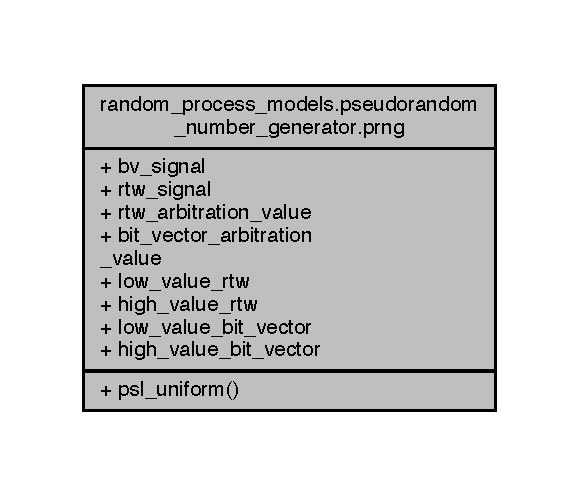
\includegraphics[width=278pt]{d0/d0d/classrandom__process__models_1_1pseudorandom__number__generator_1_1prng__coll__graph}
\end{center}
\end{figure}
\subsection*{Static Public Member Functions}
\begin{DoxyCompactItemize}
\item 
def \hyperlink{classrandom__process__models_1_1pseudorandom__number__generator_1_1prng_a1dcc8cc1bddef1852a007afc2f115f5e}{psl\+\_\+uniform}
\begin{DoxyCompactList}\small\item\em Method to generate a value for a random signal/process. \end{DoxyCompactList}\end{DoxyCompactItemize}
\subsection*{Static Public Attributes}
\begin{DoxyCompactItemize}
\item 
string \hyperlink{classrandom__process__models_1_1pseudorandom__number__generator_1_1prng_a82f57253641d85b4e2efba66fac47066}{bv\+\_\+signal} = \char`\"{}bv\char`\"{}
\item 
string \hyperlink{classrandom__process__models_1_1pseudorandom__number__generator_1_1prng_a6962172d81af8d6c172ba64e33eb0d55}{rtw\+\_\+signal} = \char`\"{}rtw\char`\"{}
\item 
float \hyperlink{classrandom__process__models_1_1pseudorandom__number__generator_1_1prng_a90c8ad6b1e19cfb7a8e9eea3f2c16728}{rtw\+\_\+arbitration\+\_\+value} = 0.\+0
\item 
float \hyperlink{classrandom__process__models_1_1pseudorandom__number__generator_1_1prng_ac3727731f4680b560c9856dce63b59b5}{bit\+\_\+vector\+\_\+arbitration\+\_\+value} = 0.\+5
\item 
int \hyperlink{classrandom__process__models_1_1pseudorandom__number__generator_1_1prng_adf3f03d77c73d020e031922b1e8ef1b4}{low\+\_\+value\+\_\+rtw} = -\/1
\item 
int \hyperlink{classrandom__process__models_1_1pseudorandom__number__generator_1_1prng_af12063b0aa05ec3b1cb998eb59af1b39}{high\+\_\+value\+\_\+rtw} = 1
\item 
int \hyperlink{classrandom__process__models_1_1pseudorandom__number__generator_1_1prng_a74806f6f1dfe673c2132e8c4ec4f0ac2}{low\+\_\+value\+\_\+bit\+\_\+vector} = 0
\item 
int \hyperlink{classrandom__process__models_1_1pseudorandom__number__generator_1_1prng_a3ff9b0f7e6c786c43774225d9ae911ce}{high\+\_\+value\+\_\+bit\+\_\+vector} = 1
\end{DoxyCompactItemize}


\subsection{Detailed Description}
Import Custom Python Packages and Modules. 

Definition at line \hyperlink{pseudorandom__number__generator_8py_source_l00087}{87} of file \hyperlink{pseudorandom__number__generator_8py_source}{pseudorandom\+\_\+number\+\_\+generator.\+py}.



\subsection{Member Function Documentation}
\hypertarget{classrandom__process__models_1_1pseudorandom__number__generator_1_1prng_a1dcc8cc1bddef1852a007afc2f115f5e}{}\index{random\+\_\+process\+\_\+models\+::pseudorandom\+\_\+number\+\_\+generator\+::prng@{random\+\_\+process\+\_\+models\+::pseudorandom\+\_\+number\+\_\+generator\+::prng}!psl\+\_\+uniform@{psl\+\_\+uniform}}
\index{psl\+\_\+uniform@{psl\+\_\+uniform}!random\+\_\+process\+\_\+models\+::pseudorandom\+\_\+number\+\_\+generator\+::prng@{random\+\_\+process\+\_\+models\+::pseudorandom\+\_\+number\+\_\+generator\+::prng}}
\subsubsection[{psl\+\_\+uniform}]{\setlength{\rightskip}{0pt plus 5cm}def random\+\_\+process\+\_\+models.\+pseudorandom\+\_\+number\+\_\+generator.\+prng.\+psl\+\_\+uniform (
\begin{DoxyParamCaption}
\item[{}]{type\+\_\+of\+\_\+signal = {\ttfamily {\bf bv\+\_\+signal}}}
\end{DoxyParamCaption}
)\hspace{0.3cm}{\ttfamily [static]}}\label{classrandom__process__models_1_1pseudorandom__number__generator_1_1prng_a1dcc8cc1bddef1852a007afc2f115f5e}


Method to generate a value for a random signal/process. 

Use the Python Standard Library\textquotesingle{}s random module to call the uniform function that is a P\+R\+N\+G based on a uniform distribution.


\begin{DoxyParams}{Parameters}
{\em type\+\_\+of\+\_\+signal} & -\/ Indicates if either of the following random signals (or random \char`\"{}processes\char`\"{}) are used.
\begin{DoxyItemize}
\item rtw, for a random telegraph wave
\begin{DoxyItemize}
\item high value\+: \char`\"{}1\char`\"{}
\item low value\+: \char`\"{}-\/1\char`\"{}
\end{DoxyItemize}
\item bv, for a bit-\/vector
\begin{DoxyItemize}
\item high value\+: \char`\"{}1\char`\"{}
\item low value\+: \char`\"{}0\char`\"{} 
\end{DoxyItemize}
\end{DoxyItemize}\\
\hline
\end{DoxyParams}
\begin{DoxyReturn}{Returns}
-\/ Nothing. O(1) method. 
\end{DoxyReturn}


Definition at line \hyperlink{pseudorandom__number__generator_8py_source_l00135}{135} of file \hyperlink{pseudorandom__number__generator_8py_source}{pseudorandom\+\_\+number\+\_\+generator.\+py}.


\begin{DoxyCode}
\hypertarget{classrandom__process__models_1_1pseudorandom__number__generator_1_1prng_l00135}{}\hyperlink{classrandom__process__models_1_1pseudorandom__number__generator_1_1prng_a1dcc8cc1bddef1852a007afc2f115f5e}{00135}     \textcolor{keyword}{def }\hyperlink{classrandom__process__models_1_1pseudorandom__number__generator_1_1prng_a1dcc8cc1bddef1852a007afc2f115f5e}{psl\_uniform}(type\_of\_signal=bv\_signal):
\end{DoxyCode}


\subsection{Member Data Documentation}
\hypertarget{classrandom__process__models_1_1pseudorandom__number__generator_1_1prng_ac3727731f4680b560c9856dce63b59b5}{}\index{random\+\_\+process\+\_\+models\+::pseudorandom\+\_\+number\+\_\+generator\+::prng@{random\+\_\+process\+\_\+models\+::pseudorandom\+\_\+number\+\_\+generator\+::prng}!bit\+\_\+vector\+\_\+arbitration\+\_\+value@{bit\+\_\+vector\+\_\+arbitration\+\_\+value}}
\index{bit\+\_\+vector\+\_\+arbitration\+\_\+value@{bit\+\_\+vector\+\_\+arbitration\+\_\+value}!random\+\_\+process\+\_\+models\+::pseudorandom\+\_\+number\+\_\+generator\+::prng@{random\+\_\+process\+\_\+models\+::pseudorandom\+\_\+number\+\_\+generator\+::prng}}
\subsubsection[{bit\+\_\+vector\+\_\+arbitration\+\_\+value}]{\setlength{\rightskip}{0pt plus 5cm}float random\+\_\+process\+\_\+models.\+pseudorandom\+\_\+number\+\_\+generator.\+prng.\+bit\+\_\+vector\+\_\+arbitration\+\_\+value = 0.\+5\hspace{0.3cm}{\ttfamily [static]}}\label{classrandom__process__models_1_1pseudorandom__number__generator_1_1prng_ac3727731f4680b560c9856dce63b59b5}


Definition at line \hyperlink{pseudorandom__number__generator_8py_source_l00110}{110} of file \hyperlink{pseudorandom__number__generator_8py_source}{pseudorandom\+\_\+number\+\_\+generator.\+py}.

\hypertarget{classrandom__process__models_1_1pseudorandom__number__generator_1_1prng_a82f57253641d85b4e2efba66fac47066}{}\index{random\+\_\+process\+\_\+models\+::pseudorandom\+\_\+number\+\_\+generator\+::prng@{random\+\_\+process\+\_\+models\+::pseudorandom\+\_\+number\+\_\+generator\+::prng}!bv\+\_\+signal@{bv\+\_\+signal}}
\index{bv\+\_\+signal@{bv\+\_\+signal}!random\+\_\+process\+\_\+models\+::pseudorandom\+\_\+number\+\_\+generator\+::prng@{random\+\_\+process\+\_\+models\+::pseudorandom\+\_\+number\+\_\+generator\+::prng}}
\subsubsection[{bv\+\_\+signal}]{\setlength{\rightskip}{0pt plus 5cm}string random\+\_\+process\+\_\+models.\+pseudorandom\+\_\+number\+\_\+generator.\+prng.\+bv\+\_\+signal = \char`\"{}bv\char`\"{}\hspace{0.3cm}{\ttfamily [static]}}\label{classrandom__process__models_1_1pseudorandom__number__generator_1_1prng_a82f57253641d85b4e2efba66fac47066}


Definition at line \hyperlink{pseudorandom__number__generator_8py_source_l00090}{90} of file \hyperlink{pseudorandom__number__generator_8py_source}{pseudorandom\+\_\+number\+\_\+generator.\+py}.

\hypertarget{classrandom__process__models_1_1pseudorandom__number__generator_1_1prng_a3ff9b0f7e6c786c43774225d9ae911ce}{}\index{random\+\_\+process\+\_\+models\+::pseudorandom\+\_\+number\+\_\+generator\+::prng@{random\+\_\+process\+\_\+models\+::pseudorandom\+\_\+number\+\_\+generator\+::prng}!high\+\_\+value\+\_\+bit\+\_\+vector@{high\+\_\+value\+\_\+bit\+\_\+vector}}
\index{high\+\_\+value\+\_\+bit\+\_\+vector@{high\+\_\+value\+\_\+bit\+\_\+vector}!random\+\_\+process\+\_\+models\+::pseudorandom\+\_\+number\+\_\+generator\+::prng@{random\+\_\+process\+\_\+models\+::pseudorandom\+\_\+number\+\_\+generator\+::prng}}
\subsubsection[{high\+\_\+value\+\_\+bit\+\_\+vector}]{\setlength{\rightskip}{0pt plus 5cm}int random\+\_\+process\+\_\+models.\+pseudorandom\+\_\+number\+\_\+generator.\+prng.\+high\+\_\+value\+\_\+bit\+\_\+vector = 1\hspace{0.3cm}{\ttfamily [static]}}\label{classrandom__process__models_1_1pseudorandom__number__generator_1_1prng_a3ff9b0f7e6c786c43774225d9ae911ce}


Definition at line \hyperlink{pseudorandom__number__generator_8py_source_l00116}{116} of file \hyperlink{pseudorandom__number__generator_8py_source}{pseudorandom\+\_\+number\+\_\+generator.\+py}.

\hypertarget{classrandom__process__models_1_1pseudorandom__number__generator_1_1prng_af12063b0aa05ec3b1cb998eb59af1b39}{}\index{random\+\_\+process\+\_\+models\+::pseudorandom\+\_\+number\+\_\+generator\+::prng@{random\+\_\+process\+\_\+models\+::pseudorandom\+\_\+number\+\_\+generator\+::prng}!high\+\_\+value\+\_\+rtw@{high\+\_\+value\+\_\+rtw}}
\index{high\+\_\+value\+\_\+rtw@{high\+\_\+value\+\_\+rtw}!random\+\_\+process\+\_\+models\+::pseudorandom\+\_\+number\+\_\+generator\+::prng@{random\+\_\+process\+\_\+models\+::pseudorandom\+\_\+number\+\_\+generator\+::prng}}
\subsubsection[{high\+\_\+value\+\_\+rtw}]{\setlength{\rightskip}{0pt plus 5cm}int random\+\_\+process\+\_\+models.\+pseudorandom\+\_\+number\+\_\+generator.\+prng.\+high\+\_\+value\+\_\+rtw = 1\hspace{0.3cm}{\ttfamily [static]}}\label{classrandom__process__models_1_1pseudorandom__number__generator_1_1prng_af12063b0aa05ec3b1cb998eb59af1b39}


Definition at line \hyperlink{pseudorandom__number__generator_8py_source_l00113}{113} of file \hyperlink{pseudorandom__number__generator_8py_source}{pseudorandom\+\_\+number\+\_\+generator.\+py}.

\hypertarget{classrandom__process__models_1_1pseudorandom__number__generator_1_1prng_a74806f6f1dfe673c2132e8c4ec4f0ac2}{}\index{random\+\_\+process\+\_\+models\+::pseudorandom\+\_\+number\+\_\+generator\+::prng@{random\+\_\+process\+\_\+models\+::pseudorandom\+\_\+number\+\_\+generator\+::prng}!low\+\_\+value\+\_\+bit\+\_\+vector@{low\+\_\+value\+\_\+bit\+\_\+vector}}
\index{low\+\_\+value\+\_\+bit\+\_\+vector@{low\+\_\+value\+\_\+bit\+\_\+vector}!random\+\_\+process\+\_\+models\+::pseudorandom\+\_\+number\+\_\+generator\+::prng@{random\+\_\+process\+\_\+models\+::pseudorandom\+\_\+number\+\_\+generator\+::prng}}
\subsubsection[{low\+\_\+value\+\_\+bit\+\_\+vector}]{\setlength{\rightskip}{0pt plus 5cm}int random\+\_\+process\+\_\+models.\+pseudorandom\+\_\+number\+\_\+generator.\+prng.\+low\+\_\+value\+\_\+bit\+\_\+vector = 0\hspace{0.3cm}{\ttfamily [static]}}\label{classrandom__process__models_1_1pseudorandom__number__generator_1_1prng_a74806f6f1dfe673c2132e8c4ec4f0ac2}


Definition at line \hyperlink{pseudorandom__number__generator_8py_source_l00115}{115} of file \hyperlink{pseudorandom__number__generator_8py_source}{pseudorandom\+\_\+number\+\_\+generator.\+py}.

\hypertarget{classrandom__process__models_1_1pseudorandom__number__generator_1_1prng_adf3f03d77c73d020e031922b1e8ef1b4}{}\index{random\+\_\+process\+\_\+models\+::pseudorandom\+\_\+number\+\_\+generator\+::prng@{random\+\_\+process\+\_\+models\+::pseudorandom\+\_\+number\+\_\+generator\+::prng}!low\+\_\+value\+\_\+rtw@{low\+\_\+value\+\_\+rtw}}
\index{low\+\_\+value\+\_\+rtw@{low\+\_\+value\+\_\+rtw}!random\+\_\+process\+\_\+models\+::pseudorandom\+\_\+number\+\_\+generator\+::prng@{random\+\_\+process\+\_\+models\+::pseudorandom\+\_\+number\+\_\+generator\+::prng}}
\subsubsection[{low\+\_\+value\+\_\+rtw}]{\setlength{\rightskip}{0pt plus 5cm}int random\+\_\+process\+\_\+models.\+pseudorandom\+\_\+number\+\_\+generator.\+prng.\+low\+\_\+value\+\_\+rtw = -\/1\hspace{0.3cm}{\ttfamily [static]}}\label{classrandom__process__models_1_1pseudorandom__number__generator_1_1prng_adf3f03d77c73d020e031922b1e8ef1b4}


Definition at line \hyperlink{pseudorandom__number__generator_8py_source_l00112}{112} of file \hyperlink{pseudorandom__number__generator_8py_source}{pseudorandom\+\_\+number\+\_\+generator.\+py}.

\hypertarget{classrandom__process__models_1_1pseudorandom__number__generator_1_1prng_a90c8ad6b1e19cfb7a8e9eea3f2c16728}{}\index{random\+\_\+process\+\_\+models\+::pseudorandom\+\_\+number\+\_\+generator\+::prng@{random\+\_\+process\+\_\+models\+::pseudorandom\+\_\+number\+\_\+generator\+::prng}!rtw\+\_\+arbitration\+\_\+value@{rtw\+\_\+arbitration\+\_\+value}}
\index{rtw\+\_\+arbitration\+\_\+value@{rtw\+\_\+arbitration\+\_\+value}!random\+\_\+process\+\_\+models\+::pseudorandom\+\_\+number\+\_\+generator\+::prng@{random\+\_\+process\+\_\+models\+::pseudorandom\+\_\+number\+\_\+generator\+::prng}}
\subsubsection[{rtw\+\_\+arbitration\+\_\+value}]{\setlength{\rightskip}{0pt plus 5cm}float random\+\_\+process\+\_\+models.\+pseudorandom\+\_\+number\+\_\+generator.\+prng.\+rtw\+\_\+arbitration\+\_\+value = 0.\+0\hspace{0.3cm}{\ttfamily [static]}}\label{classrandom__process__models_1_1pseudorandom__number__generator_1_1prng_a90c8ad6b1e19cfb7a8e9eea3f2c16728}


Definition at line \hyperlink{pseudorandom__number__generator_8py_source_l00101}{101} of file \hyperlink{pseudorandom__number__generator_8py_source}{pseudorandom\+\_\+number\+\_\+generator.\+py}.

\hypertarget{classrandom__process__models_1_1pseudorandom__number__generator_1_1prng_a6962172d81af8d6c172ba64e33eb0d55}{}\index{random\+\_\+process\+\_\+models\+::pseudorandom\+\_\+number\+\_\+generator\+::prng@{random\+\_\+process\+\_\+models\+::pseudorandom\+\_\+number\+\_\+generator\+::prng}!rtw\+\_\+signal@{rtw\+\_\+signal}}
\index{rtw\+\_\+signal@{rtw\+\_\+signal}!random\+\_\+process\+\_\+models\+::pseudorandom\+\_\+number\+\_\+generator\+::prng@{random\+\_\+process\+\_\+models\+::pseudorandom\+\_\+number\+\_\+generator\+::prng}}
\subsubsection[{rtw\+\_\+signal}]{\setlength{\rightskip}{0pt plus 5cm}string random\+\_\+process\+\_\+models.\+pseudorandom\+\_\+number\+\_\+generator.\+prng.\+rtw\+\_\+signal = \char`\"{}rtw\char`\"{}\hspace{0.3cm}{\ttfamily [static]}}\label{classrandom__process__models_1_1pseudorandom__number__generator_1_1prng_a6962172d81af8d6c172ba64e33eb0d55}


Definition at line \hyperlink{pseudorandom__number__generator_8py_source_l00092}{92} of file \hyperlink{pseudorandom__number__generator_8py_source}{pseudorandom\+\_\+number\+\_\+generator.\+py}.



The documentation for this class was generated from the following file\+:\begin{DoxyCompactItemize}
\item 
random\+\_\+process\+\_\+models/\hyperlink{pseudorandom__number__generator_8py}{pseudorandom\+\_\+number\+\_\+generator.\+py}\end{DoxyCompactItemize}

\hypertarget{classrandom__process__models_1_1pseudorandom__number__generator__tester_1_1prng__tester}{}\section{random\+\_\+process\+\_\+models.\+pseudorandom\+\_\+number\+\_\+generator\+\_\+tester.\+prng\+\_\+tester Class Reference}
\label{classrandom__process__models_1_1pseudorandom__number__generator__tester_1_1prng__tester}\index{random\+\_\+process\+\_\+models.\+pseudorandom\+\_\+number\+\_\+generator\+\_\+tester.\+prng\+\_\+tester@{random\+\_\+process\+\_\+models.\+pseudorandom\+\_\+number\+\_\+generator\+\_\+tester.\+prng\+\_\+tester}}


Module with methods that perform miscellaneous tasks.  




Collaboration diagram for random\+\_\+process\+\_\+models.\+pseudorandom\+\_\+number\+\_\+generator\+\_\+tester.\+prng\+\_\+tester\+:
\nopagebreak
\begin{figure}[H]
\begin{center}
\leavevmode

\includegraphics[width=278pt]{de/d6a/classrandom__process__models_1_1pseudorandom__number__generator__tester_1_1prng__tester__coll__graph}
\end{center}
\end{figure}
\subsection*{Static Public Member Functions}
\begin{DoxyCompactItemize}
\item 
def \hyperlink{classrandom__process__models_1_1pseudorandom__number__generator__tester_1_1prng__tester_a5597ea984257dcd64376064fda82385d}{test\+\_\+psl\+\_\+uniform} ()
\begin{DoxyCompactList}\small\item\em ========================================================= Method to test the methods that uses the P\+R\+N\+G from Python Standard Library to produce random numbers. \end{DoxyCompactList}\item 
def \hyperlink{classrandom__process__models_1_1pseudorandom__number__generator__tester_1_1prng__tester_aff9e5a07e94168e1eabd25b7f3a4eb32}{test\+\_\+prng\+\_\+methods} ()
\begin{DoxyCompactList}\small\item\em ========================================================= Method to test the miscellaneous methods. \end{DoxyCompactList}\end{DoxyCompactItemize}


\subsection{Detailed Description}
Module with methods that perform miscellaneous tasks. 



Definition at line \hyperlink{pseudorandom__number__generator__tester_8py_source_l00087}{87} of file \hyperlink{pseudorandom__number__generator__tester_8py_source}{pseudorandom\+\_\+number\+\_\+generator\+\_\+tester.\+py}.



\subsection{Member Function Documentation}
\hypertarget{classrandom__process__models_1_1pseudorandom__number__generator__tester_1_1prng__tester_aff9e5a07e94168e1eabd25b7f3a4eb32}{}\index{random\+\_\+process\+\_\+models\+::pseudorandom\+\_\+number\+\_\+generator\+\_\+tester\+::prng\+\_\+tester@{random\+\_\+process\+\_\+models\+::pseudorandom\+\_\+number\+\_\+generator\+\_\+tester\+::prng\+\_\+tester}!test\+\_\+prng\+\_\+methods@{test\+\_\+prng\+\_\+methods}}
\index{test\+\_\+prng\+\_\+methods@{test\+\_\+prng\+\_\+methods}!random\+\_\+process\+\_\+models\+::pseudorandom\+\_\+number\+\_\+generator\+\_\+tester\+::prng\+\_\+tester@{random\+\_\+process\+\_\+models\+::pseudorandom\+\_\+number\+\_\+generator\+\_\+tester\+::prng\+\_\+tester}}
\subsubsection[{test\+\_\+prng\+\_\+methods()}]{\setlength{\rightskip}{0pt plus 5cm}def random\+\_\+process\+\_\+models.\+pseudorandom\+\_\+number\+\_\+generator\+\_\+tester.\+prng\+\_\+tester.\+test\+\_\+prng\+\_\+methods (
\begin{DoxyParamCaption}
{}
\end{DoxyParamCaption}
)\hspace{0.3cm}{\ttfamily [static]}}\label{classrandom__process__models_1_1pseudorandom__number__generator__tester_1_1prng__tester_aff9e5a07e94168e1eabd25b7f3a4eb32}


========================================================= Method to test the miscellaneous methods. 


\begin{DoxyParams}{Parameters}
{\em -\/} & Nothing \\
\hline
\end{DoxyParams}
\begin{DoxyReturn}{Returns}
-\/ Nothing. O(1) method. 
\end{DoxyReturn}


Definition at line \hyperlink{pseudorandom__number__generator__tester_8py_source_l00127}{127} of file \hyperlink{pseudorandom__number__generator__tester_8py_source}{pseudorandom\+\_\+number\+\_\+generator\+\_\+tester.\+py}.


\begin{DoxyCode}
\hypertarget{classrandom__process__models_1_1pseudorandom__number__generator__tester_1_1prng__tester_l00127}{}\hyperlink{classrandom__process__models_1_1pseudorandom__number__generator__tester_1_1prng__tester_aff9e5a07e94168e1eabd25b7f3a4eb32}{00127}     \textcolor{keyword}{def }\hyperlink{classrandom__process__models_1_1pseudorandom__number__generator__tester_1_1prng__tester_aff9e5a07e94168e1eabd25b7f3a4eb32}{test\_prng\_methods}():
00128         print(\textcolor{stringliteral}{""})
00129         print(\textcolor{stringliteral}{""})
00130         print(\textcolor{stringliteral}{"==   Testing class: misc\_tester."})
00131         prng\_tester.test\_psl\_uniform()
00132 \end{DoxyCode}
\hypertarget{classrandom__process__models_1_1pseudorandom__number__generator__tester_1_1prng__tester_a5597ea984257dcd64376064fda82385d}{}\index{random\+\_\+process\+\_\+models\+::pseudorandom\+\_\+number\+\_\+generator\+\_\+tester\+::prng\+\_\+tester@{random\+\_\+process\+\_\+models\+::pseudorandom\+\_\+number\+\_\+generator\+\_\+tester\+::prng\+\_\+tester}!test\+\_\+psl\+\_\+uniform@{test\+\_\+psl\+\_\+uniform}}
\index{test\+\_\+psl\+\_\+uniform@{test\+\_\+psl\+\_\+uniform}!random\+\_\+process\+\_\+models\+::pseudorandom\+\_\+number\+\_\+generator\+\_\+tester\+::prng\+\_\+tester@{random\+\_\+process\+\_\+models\+::pseudorandom\+\_\+number\+\_\+generator\+\_\+tester\+::prng\+\_\+tester}}
\subsubsection[{test\+\_\+psl\+\_\+uniform()}]{\setlength{\rightskip}{0pt plus 5cm}def random\+\_\+process\+\_\+models.\+pseudorandom\+\_\+number\+\_\+generator\+\_\+tester.\+prng\+\_\+tester.\+test\+\_\+psl\+\_\+uniform (
\begin{DoxyParamCaption}
{}
\end{DoxyParamCaption}
)\hspace{0.3cm}{\ttfamily [static]}}\label{classrandom__process__models_1_1pseudorandom__number__generator__tester_1_1prng__tester_a5597ea984257dcd64376064fda82385d}


========================================================= Method to test the methods that uses the P\+R\+N\+G from Python Standard Library to produce random numbers. 


\begin{DoxyParams}{Parameters}
{\em -\/} & Nothing \\
\hline
\end{DoxyParams}
\begin{DoxyReturn}{Returns}
-\/ Nothing. O(1) method. 
\end{DoxyReturn}


Definition at line \hyperlink{pseudorandom__number__generator__tester_8py_source_l00095}{95} of file \hyperlink{pseudorandom__number__generator__tester_8py_source}{pseudorandom\+\_\+number\+\_\+generator\+\_\+tester.\+py}.


\begin{DoxyCode}
\hypertarget{classrandom__process__models_1_1pseudorandom__number__generator__tester_1_1prng__tester_l00095}{}\hyperlink{classrandom__process__models_1_1pseudorandom__number__generator__tester_1_1prng__tester_a5597ea984257dcd64376064fda82385d}{00095}     \textcolor{keyword}{def }\hyperlink{classrandom__process__models_1_1pseudorandom__number__generator__tester_1_1prng__tester_a5597ea984257dcd64376064fda82385d}{test\_psl\_uniform}():
00096         print(\textcolor{stringliteral}{" Testing the psl\_uniform()."})
00097         prompt = \textcolor{stringliteral}{"  ... Test: incorrect type of signal, 'whatever'.     \{\}"}
00098         statistical\_analysis.increment\_number\_test\_cases\_used()
00099         temp\_ran\_number = prng.psl\_uniform(\textcolor{stringliteral}{"whatever"})
00100         \textcolor{keywordflow}{if} (1==temp\_ran\_number) \textcolor{keywordflow}{or} (0==temp\_ran\_number):
00101             print(prompt .format(\textcolor{stringliteral}{"OK"}))
00102             statistical\_analysis.increment\_number\_test\_cases\_passed()
00103         \textcolor{keywordflow}{else}:
00104             print(prompt .format(\textcolor{stringliteral}{"FAIL!!!"}))
00105         prompt = \textcolor{stringliteral}{"  ... Test: for bit vector signal, 'bv'.          \{\}"}
00106         statistical\_analysis.increment\_number\_test\_cases\_used()
00107         temp\_ran\_number = prng.psl\_uniform(prng.bv\_signal)
00108         \textcolor{keywordflow}{if} (1==temp\_ran\_number) \textcolor{keywordflow}{or} (0==temp\_ran\_number):
00109             print(prompt .format(\textcolor{stringliteral}{"OK"}))
00110             statistical\_analysis.increment\_number\_test\_cases\_passed()
00111         \textcolor{keywordflow}{else}:
00112             print(prompt .format(\textcolor{stringliteral}{"FAIL!!!"}))
00113         prompt = \textcolor{stringliteral}{"  ... Test: for RTW signal, 'rtw'.        \{\}"}
00114         statistical\_analysis.increment\_number\_test\_cases\_used()
00115         temp\_ran\_number = prng.psl\_uniform(prng.rtw\_signal)
00116         \textcolor{keywordflow}{if} (1==temp\_ran\_number) \textcolor{keywordflow}{or} (-1==temp\_ran\_number):
00117             print(prompt .format(\textcolor{stringliteral}{"  OK"}))
00118             statistical\_analysis.increment\_number\_test\_cases\_passed()
00119         \textcolor{keywordflow}{else}:
00120             print(prompt .format(\textcolor{stringliteral}{"FAIL!!!"}))
\end{DoxyCode}


The documentation for this class was generated from the following file\+:\begin{DoxyCompactItemize}
\item 
random\+\_\+process\+\_\+models/\hyperlink{pseudorandom__number__generator__tester_8py}{pseudorandom\+\_\+number\+\_\+generator\+\_\+tester.\+py}\end{DoxyCompactItemize}

\hypertarget{classutilities_1_1queue__ip__arguments_1_1queue__ip__args}{}\section{utilities.\+queue\+\_\+ip\+\_\+arguments.\+queue\+\_\+ip\+\_\+args Class Reference}
\label{classutilities_1_1queue__ip__arguments_1_1queue__ip__args}\index{utilities.\+queue\+\_\+ip\+\_\+arguments.\+queue\+\_\+ip\+\_\+args@{utilities.\+queue\+\_\+ip\+\_\+arguments.\+queue\+\_\+ip\+\_\+args}}


Import Custom Python Modules.  




Collaboration diagram for utilities.\+queue\+\_\+ip\+\_\+arguments.\+queue\+\_\+ip\+\_\+args\+:
\nopagebreak
\begin{figure}[H]
\begin{center}
\leavevmode

\includegraphics[width=236pt]{d0/dae/classutilities_1_1queue__ip__arguments_1_1queue__ip__args__coll__graph}
\end{center}
\end{figure}
\subsection*{Static Public Member Functions}
\begin{DoxyCompactItemize}
\item 
def \hyperlink{classutilities_1_1queue__ip__arguments_1_1queue__ip__args_a1ace4b3c7b9a9e97a872c3a04337442c}{get\+\_\+list\+\_\+of\+\_\+input\+\_\+arguments} ()
\begin{DoxyCompactList}\small\item\em Method to get the list of input arguments. \end{DoxyCompactList}\item 
def \hyperlink{classutilities_1_1queue__ip__arguments_1_1queue__ip__args_a85480b443e2538123e8531852f9035c9}{print\+\_\+all\+\_\+input\+\_\+arguments} ()
\begin{DoxyCompactList}\small\item\em Method to print all the input arguments. \end{DoxyCompactList}\item 
def \hyperlink{classutilities_1_1queue__ip__arguments_1_1queue__ip__args_a7b3c5efad539fadfb53eda0cfb8d3f03}{get\+\_\+1st\+\_\+input\+\_\+argument} ()
\begin{DoxyCompactList}\small\item\em Method to get the first input argument. \end{DoxyCompactList}\item 
def \hyperlink{classutilities_1_1queue__ip__arguments_1_1queue__ip__args_a18e59da1e2c8044e79ca32a5455ef40b}{get\+\_\+2nd\+\_\+input\+\_\+argument} ()
\begin{DoxyCompactList}\small\item\em Method to get the second input argument. \end{DoxyCompactList}\item 
def \hyperlink{classutilities_1_1queue__ip__arguments_1_1queue__ip__args_ab95a4242fd55bf5d126b35a5f5172593}{get\+\_\+number\+\_\+of\+\_\+input\+\_\+arguments} ()
\begin{DoxyCompactList}\small\item\em Method to get the number of input arguments. \end{DoxyCompactList}\item 
def \hyperlink{classutilities_1_1queue__ip__arguments_1_1queue__ip__args_a4b34415e7ff12abecd89b1e10755aa8d}{set\+\_\+input\+\_\+arguments} (list\+\_\+of\+\_\+ip\+\_\+arguments)
\begin{DoxyCompactList}\small\item\em Method to set the input arguments. \end{DoxyCompactList}\item 
def \hyperlink{classutilities_1_1queue__ip__arguments_1_1queue__ip__args_a1a87ae4035acfa51fe1d1aff53f770f3}{check\+\_\+if\+\_\+help\+\_\+wanted} ()
\begin{DoxyCompactList}\small\item\em Method to determine if the user wants help, and conequently display the user manual. \end{DoxyCompactList}\item 
def \hyperlink{classutilities_1_1queue__ip__arguments_1_1queue__ip__args_a5fecd33a91d20f19acba2fb1b8d1a60e}{how\+\_\+to\+\_\+use\+\_\+script} ()
\begin{DoxyCompactList}\small\item\em Method to provide information on how to run this script. \end{DoxyCompactList}\item 
def \hyperlink{classutilities_1_1queue__ip__arguments_1_1queue__ip__args_a28c79307da87e28e9ac3467290fd5738}{print\+\_\+help\+\_\+option} ()
\begin{DoxyCompactList}\small\item\em Method to print the help option to access the user manual. \end{DoxyCompactList}\item 
def \hyperlink{classutilities_1_1queue__ip__arguments_1_1queue__ip__args_afdfbfffba8afb5e786283dd22d856e93}{input\+\_\+arguments\+\_\+error} ()
\begin{DoxyCompactList}\small\item\em Method to indicate error wth input arguments. \end{DoxyCompactList}\item 
def \hyperlink{classutilities_1_1queue__ip__arguments_1_1queue__ip__args_ae1fc6d7af2e429d0656dbf388711db94}{process\+\_\+1st\+\_\+ip\+\_\+arg} ()
\begin{DoxyCompactList}\small\item\em Method to process the first input argument. \end{DoxyCompactList}\item 
def \hyperlink{classutilities_1_1queue__ip__arguments_1_1queue__ip__args_a82d245379c48196f61d4268882dd5c6d}{process\+\_\+2nd\+\_\+ip\+\_\+arg} ()
\begin{DoxyCompactList}\small\item\em Method to process the second input argument. \end{DoxyCompactList}\end{DoxyCompactItemize}
\subsection*{Static Public Attributes}
\begin{DoxyCompactItemize}
\item 
list \hyperlink{classutilities_1_1queue__ip__arguments_1_1queue__ip__args_acc8e7685be71a7f95ede7c980355c9f3}{set\+\_\+of\+\_\+input\+\_\+arguments} = \mbox{[}$\,$\mbox{]}
\item 
string \hyperlink{classutilities_1_1queue__ip__arguments_1_1queue__ip__args_a14394c9820086e09d5b926d9910a180f}{first\+\_\+input\+\_\+argument} = \char`\"{}First input argument.\char`\"{}
\item 
string \hyperlink{classutilities_1_1queue__ip__arguments_1_1queue__ip__args_a0b179a70c0e57de2794d0d532e534c9c}{second\+\_\+input\+\_\+argument} = \char`\"{}Second input argument.\char`\"{}
\item 
string \hyperlink{classutilities_1_1queue__ip__arguments_1_1queue__ip__args_a8d93f9ade7608583602a9948c0d744f7}{json\+\_\+f\+\_\+ext} = \char`\"{}.json\char`\"{}
\end{DoxyCompactItemize}


\subsection{Detailed Description}
Import Custom Python Modules. 

Module with methods that clean Bib\+Te\+X files. 

Definition at line \hyperlink{queue__ip__arguments_8py_source_l00072}{72} of file \hyperlink{queue__ip__arguments_8py_source}{queue\+\_\+ip\+\_\+arguments.\+py}.



\subsection{Member Function Documentation}
\hypertarget{classutilities_1_1queue__ip__arguments_1_1queue__ip__args_a1a87ae4035acfa51fe1d1aff53f770f3}{}\index{utilities\+::queue\+\_\+ip\+\_\+arguments\+::queue\+\_\+ip\+\_\+args@{utilities\+::queue\+\_\+ip\+\_\+arguments\+::queue\+\_\+ip\+\_\+args}!check\+\_\+if\+\_\+help\+\_\+wanted@{check\+\_\+if\+\_\+help\+\_\+wanted}}
\index{check\+\_\+if\+\_\+help\+\_\+wanted@{check\+\_\+if\+\_\+help\+\_\+wanted}!utilities\+::queue\+\_\+ip\+\_\+arguments\+::queue\+\_\+ip\+\_\+args@{utilities\+::queue\+\_\+ip\+\_\+arguments\+::queue\+\_\+ip\+\_\+args}}
\subsubsection[{check\+\_\+if\+\_\+help\+\_\+wanted()}]{\setlength{\rightskip}{0pt plus 5cm}def utilities.\+queue\+\_\+ip\+\_\+arguments.\+queue\+\_\+ip\+\_\+args.\+check\+\_\+if\+\_\+help\+\_\+wanted (
\begin{DoxyParamCaption}
{}
\end{DoxyParamCaption}
)\hspace{0.3cm}{\ttfamily [static]}}\label{classutilities_1_1queue__ip__arguments_1_1queue__ip__args_a1a87ae4035acfa51fe1d1aff53f770f3}


Method to determine if the user wants help, and conequently display the user manual. 

O(n) method, with respect to the number of input arguments. 

Definition at line \hyperlink{queue__ip__arguments_8py_source_l00158}{158} of file \hyperlink{queue__ip__arguments_8py_source}{queue\+\_\+ip\+\_\+arguments.\+py}.


\begin{DoxyCode}
\hypertarget{classutilities_1_1queue__ip__arguments_1_1queue__ip__args_l00158}{}\hyperlink{classutilities_1_1queue__ip__arguments_1_1queue__ip__args_a1a87ae4035acfa51fe1d1aff53f770f3}{00158}     \textcolor{keyword}{def }\hyperlink{classutilities_1_1queue__ip__arguments_1_1queue__ip__args_a1a87ae4035acfa51fe1d1aff53f770f3}{check\_if\_help\_wanted}():
00159         \textcolor{comment}{# If user wants to read the brief user manual,}
00160         \textcolor{keywordflow}{if} \textcolor{stringliteral}{"-h"} \textcolor{keywordflow}{in} queue\_ip\_args.set\_of\_input\_arguments:
00161             \textcolor{comment}{# Display the user manual and exit.}
00162             queue\_ip\_args.how\_to\_use\_script()
00163             sys.exit()
\end{DoxyCode}
\hypertarget{classutilities_1_1queue__ip__arguments_1_1queue__ip__args_a7b3c5efad539fadfb53eda0cfb8d3f03}{}\index{utilities\+::queue\+\_\+ip\+\_\+arguments\+::queue\+\_\+ip\+\_\+args@{utilities\+::queue\+\_\+ip\+\_\+arguments\+::queue\+\_\+ip\+\_\+args}!get\+\_\+1st\+\_\+input\+\_\+argument@{get\+\_\+1st\+\_\+input\+\_\+argument}}
\index{get\+\_\+1st\+\_\+input\+\_\+argument@{get\+\_\+1st\+\_\+input\+\_\+argument}!utilities\+::queue\+\_\+ip\+\_\+arguments\+::queue\+\_\+ip\+\_\+args@{utilities\+::queue\+\_\+ip\+\_\+arguments\+::queue\+\_\+ip\+\_\+args}}
\subsubsection[{get\+\_\+1st\+\_\+input\+\_\+argument()}]{\setlength{\rightskip}{0pt plus 5cm}def utilities.\+queue\+\_\+ip\+\_\+arguments.\+queue\+\_\+ip\+\_\+args.\+get\+\_\+1st\+\_\+input\+\_\+argument (
\begin{DoxyParamCaption}
{}
\end{DoxyParamCaption}
)\hspace{0.3cm}{\ttfamily [static]}}\label{classutilities_1_1queue__ip__arguments_1_1queue__ip__args_a7b3c5efad539fadfb53eda0cfb8d3f03}


Method to get the first input argument. 

\begin{DoxyReturn}{Returns}
-\/ First input argument for the program. O(1) method. 
\end{DoxyReturn}


Definition at line \hyperlink{queue__ip__arguments_8py_source_l00108}{108} of file \hyperlink{queue__ip__arguments_8py_source}{queue\+\_\+ip\+\_\+arguments.\+py}.


\begin{DoxyCode}
\hypertarget{classutilities_1_1queue__ip__arguments_1_1queue__ip__args_l00108}{}\hyperlink{classutilities_1_1queue__ip__arguments_1_1queue__ip__args_a7b3c5efad539fadfb53eda0cfb8d3f03}{00108}     \textcolor{keyword}{def }\hyperlink{classutilities_1_1queue__ip__arguments_1_1queue__ip__args_a7b3c5efad539fadfb53eda0cfb8d3f03}{get\_1st\_input\_argument}():
00109         \textcolor{keywordflow}{if} 0 < len(queue\_ip\_args.get\_list\_of\_input\_arguments()):
00110             \textcolor{keywordflow}{return} queue\_ip\_args.set\_of\_input\_arguments[0]
00111         \textcolor{keywordflow}{else}:
00112             warnings.warn(\textcolor{stringliteral}{" 1st input argument is missing!!!"})
00113             queue\_ip\_args.input\_arguments\_error()
\end{DoxyCode}
\hypertarget{classutilities_1_1queue__ip__arguments_1_1queue__ip__args_a18e59da1e2c8044e79ca32a5455ef40b}{}\index{utilities\+::queue\+\_\+ip\+\_\+arguments\+::queue\+\_\+ip\+\_\+args@{utilities\+::queue\+\_\+ip\+\_\+arguments\+::queue\+\_\+ip\+\_\+args}!get\+\_\+2nd\+\_\+input\+\_\+argument@{get\+\_\+2nd\+\_\+input\+\_\+argument}}
\index{get\+\_\+2nd\+\_\+input\+\_\+argument@{get\+\_\+2nd\+\_\+input\+\_\+argument}!utilities\+::queue\+\_\+ip\+\_\+arguments\+::queue\+\_\+ip\+\_\+args@{utilities\+::queue\+\_\+ip\+\_\+arguments\+::queue\+\_\+ip\+\_\+args}}
\subsubsection[{get\+\_\+2nd\+\_\+input\+\_\+argument()}]{\setlength{\rightskip}{0pt plus 5cm}def utilities.\+queue\+\_\+ip\+\_\+arguments.\+queue\+\_\+ip\+\_\+args.\+get\+\_\+2nd\+\_\+input\+\_\+argument (
\begin{DoxyParamCaption}
{}
\end{DoxyParamCaption}
)\hspace{0.3cm}{\ttfamily [static]}}\label{classutilities_1_1queue__ip__arguments_1_1queue__ip__args_a18e59da1e2c8044e79ca32a5455ef40b}


Method to get the second input argument. 

\begin{DoxyReturn}{Returns}
-\/ Second input argument for the program. O(1) method. 
\end{DoxyReturn}


Definition at line \hyperlink{queue__ip__arguments_8py_source_l00119}{119} of file \hyperlink{queue__ip__arguments_8py_source}{queue\+\_\+ip\+\_\+arguments.\+py}.


\begin{DoxyCode}
\hypertarget{classutilities_1_1queue__ip__arguments_1_1queue__ip__args_l00119}{}\hyperlink{classutilities_1_1queue__ip__arguments_1_1queue__ip__args_a18e59da1e2c8044e79ca32a5455ef40b}{00119}     \textcolor{keyword}{def }\hyperlink{classutilities_1_1queue__ip__arguments_1_1queue__ip__args_a18e59da1e2c8044e79ca32a5455ef40b}{get\_2nd\_input\_argument}():
00120         \textcolor{keywordflow}{if} 1 < len(queue\_ip\_args.get\_list\_of\_input\_arguments()):
00121             \textcolor{keywordflow}{return} queue\_ip\_args.set\_of\_input\_arguments[1]
00122         \textcolor{keywordflow}{else}:
00123             warnings.warn(\textcolor{stringliteral}{" 2nd input argument is missing!!!"})
00124             queue\_ip\_args.input\_arguments\_error()
\end{DoxyCode}
\hypertarget{classutilities_1_1queue__ip__arguments_1_1queue__ip__args_a1ace4b3c7b9a9e97a872c3a04337442c}{}\index{utilities\+::queue\+\_\+ip\+\_\+arguments\+::queue\+\_\+ip\+\_\+args@{utilities\+::queue\+\_\+ip\+\_\+arguments\+::queue\+\_\+ip\+\_\+args}!get\+\_\+list\+\_\+of\+\_\+input\+\_\+arguments@{get\+\_\+list\+\_\+of\+\_\+input\+\_\+arguments}}
\index{get\+\_\+list\+\_\+of\+\_\+input\+\_\+arguments@{get\+\_\+list\+\_\+of\+\_\+input\+\_\+arguments}!utilities\+::queue\+\_\+ip\+\_\+arguments\+::queue\+\_\+ip\+\_\+args@{utilities\+::queue\+\_\+ip\+\_\+arguments\+::queue\+\_\+ip\+\_\+args}}
\subsubsection[{get\+\_\+list\+\_\+of\+\_\+input\+\_\+arguments()}]{\setlength{\rightskip}{0pt plus 5cm}def utilities.\+queue\+\_\+ip\+\_\+arguments.\+queue\+\_\+ip\+\_\+args.\+get\+\_\+list\+\_\+of\+\_\+input\+\_\+arguments (
\begin{DoxyParamCaption}
{}
\end{DoxyParamCaption}
)\hspace{0.3cm}{\ttfamily [static]}}\label{classutilities_1_1queue__ip__arguments_1_1queue__ip__args_a1ace4b3c7b9a9e97a872c3a04337442c}


Method to get the list of input arguments. 

\begin{DoxyReturn}{Returns}
-\/ List of input arguments to the program. O(1) method. \begin{DoxyVerb}print "=    Set_of_input_arguments:"
for cur_ip_arg in queue_ip_args.set_of_input_arguments:
    print " "+cur_ip_arg
\end{DoxyVerb}
 
\end{DoxyReturn}


Definition at line \hyperlink{queue__ip__arguments_8py_source_l00088}{88} of file \hyperlink{queue__ip__arguments_8py_source}{queue\+\_\+ip\+\_\+arguments.\+py}.


\begin{DoxyCode}
\hypertarget{classutilities_1_1queue__ip__arguments_1_1queue__ip__args_l00088}{}\hyperlink{classutilities_1_1queue__ip__arguments_1_1queue__ip__args_a1ace4b3c7b9a9e97a872c3a04337442c}{00088}     \textcolor{keyword}{def }\hyperlink{classutilities_1_1queue__ip__arguments_1_1queue__ip__args_a1ace4b3c7b9a9e97a872c3a04337442c}{get\_list\_of\_input\_arguments}():
00089         \textcolor{stringliteral}{"""}
00090 \textcolor{stringliteral}{        print "=    Set\_of\_input\_arguments:"}
00091 \textcolor{stringliteral}{        for cur\_ip\_arg in queue\_ip\_args.set\_of\_input\_arguments:}
00092 \textcolor{stringliteral}{            print " "+cur\_ip\_arg}
00093 \textcolor{stringliteral}{        """}
00094         \textcolor{keywordflow}{return} queue\_ip\_args.set\_of\_input\_arguments
\end{DoxyCode}
\hypertarget{classutilities_1_1queue__ip__arguments_1_1queue__ip__args_ab95a4242fd55bf5d126b35a5f5172593}{}\index{utilities\+::queue\+\_\+ip\+\_\+arguments\+::queue\+\_\+ip\+\_\+args@{utilities\+::queue\+\_\+ip\+\_\+arguments\+::queue\+\_\+ip\+\_\+args}!get\+\_\+number\+\_\+of\+\_\+input\+\_\+arguments@{get\+\_\+number\+\_\+of\+\_\+input\+\_\+arguments}}
\index{get\+\_\+number\+\_\+of\+\_\+input\+\_\+arguments@{get\+\_\+number\+\_\+of\+\_\+input\+\_\+arguments}!utilities\+::queue\+\_\+ip\+\_\+arguments\+::queue\+\_\+ip\+\_\+args@{utilities\+::queue\+\_\+ip\+\_\+arguments\+::queue\+\_\+ip\+\_\+args}}
\subsubsection[{get\+\_\+number\+\_\+of\+\_\+input\+\_\+arguments()}]{\setlength{\rightskip}{0pt plus 5cm}def utilities.\+queue\+\_\+ip\+\_\+arguments.\+queue\+\_\+ip\+\_\+args.\+get\+\_\+number\+\_\+of\+\_\+input\+\_\+arguments (
\begin{DoxyParamCaption}
{}
\end{DoxyParamCaption}
)\hspace{0.3cm}{\ttfamily [static]}}\label{classutilities_1_1queue__ip__arguments_1_1queue__ip__args_ab95a4242fd55bf5d126b35a5f5172593}


Method to get the number of input arguments. 

\begin{DoxyReturn}{Returns}
-\/ Number of input arguments for the program. O(1) method. 
\end{DoxyReturn}


Definition at line \hyperlink{queue__ip__arguments_8py_source_l00130}{130} of file \hyperlink{queue__ip__arguments_8py_source}{queue\+\_\+ip\+\_\+arguments.\+py}.


\begin{DoxyCode}
\hypertarget{classutilities_1_1queue__ip__arguments_1_1queue__ip__args_l00130}{}\hyperlink{classutilities_1_1queue__ip__arguments_1_1queue__ip__args_ab95a4242fd55bf5d126b35a5f5172593}{00130}     \textcolor{keyword}{def }\hyperlink{classutilities_1_1queue__ip__arguments_1_1queue__ip__args_ab95a4242fd55bf5d126b35a5f5172593}{get\_number\_of\_input\_arguments}():
00131         \textcolor{keywordflow}{return} len(queue\_ip\_args.set\_of\_input\_arguments)
\end{DoxyCode}
\hypertarget{classutilities_1_1queue__ip__arguments_1_1queue__ip__args_a5fecd33a91d20f19acba2fb1b8d1a60e}{}\index{utilities\+::queue\+\_\+ip\+\_\+arguments\+::queue\+\_\+ip\+\_\+args@{utilities\+::queue\+\_\+ip\+\_\+arguments\+::queue\+\_\+ip\+\_\+args}!how\+\_\+to\+\_\+use\+\_\+script@{how\+\_\+to\+\_\+use\+\_\+script}}
\index{how\+\_\+to\+\_\+use\+\_\+script@{how\+\_\+to\+\_\+use\+\_\+script}!utilities\+::queue\+\_\+ip\+\_\+arguments\+::queue\+\_\+ip\+\_\+args@{utilities\+::queue\+\_\+ip\+\_\+arguments\+::queue\+\_\+ip\+\_\+args}}
\subsubsection[{how\+\_\+to\+\_\+use\+\_\+script()}]{\setlength{\rightskip}{0pt plus 5cm}def utilities.\+queue\+\_\+ip\+\_\+arguments.\+queue\+\_\+ip\+\_\+args.\+how\+\_\+to\+\_\+use\+\_\+script (
\begin{DoxyParamCaption}
{}
\end{DoxyParamCaption}
)\hspace{0.3cm}{\ttfamily [static]}}\label{classutilities_1_1queue__ip__arguments_1_1queue__ip__args_a5fecd33a91d20f19acba2fb1b8d1a60e}


Method to provide information on how to run this script. 

O(1) method. 

Definition at line \hyperlink{queue__ip__arguments_8py_source_l00168}{168} of file \hyperlink{queue__ip__arguments_8py_source}{queue\+\_\+ip\+\_\+arguments.\+py}.


\begin{DoxyCode}
\hypertarget{classutilities_1_1queue__ip__arguments_1_1queue__ip__args_l00168}{}\hyperlink{classutilities_1_1queue__ip__arguments_1_1queue__ip__args_a5fecd33a91d20f19acba2fb1b8d1a60e}{00168}     \textcolor{keyword}{def }\hyperlink{classutilities_1_1queue__ip__arguments_1_1queue__ip__args_a5fecd33a91d20f19acba2fb1b8d1a60e}{how\_to\_use\_script}():
00169         print(\textcolor{stringliteral}{"-------------------------------------------------"})
00170         print(\textcolor{stringliteral}{"==>  This script performs genetic technology mapping."})
00171         print(\textcolor{stringliteral}{""})
00172         print(\textcolor{stringliteral}{"This script can be executed as follows:"})
00173         print(\textcolor{stringliteral}{"./problem1\_solution.py [input JSON netlist] [output JSON technology mapping] [-h]"})
00174         print(\textcolor{stringliteral}{""})
00175         print(\textcolor{stringliteral}{"==>  This other script performs incremental regression testing"})
00176         print(\textcolor{stringliteral}{" of my solution for genetic technology mapping."})
00177         print(\textcolor{stringliteral}{""})
00178         print(\textcolor{stringliteral}{"This other script can be executed as follows:"})
00179         print(\textcolor{stringliteral}{"./incremental\_test.py [input JSON netlist] [output JSON technology mapping] [-h]"})
00180         queue\_ip\_args.print\_help\_option()
00181         print(\textcolor{stringliteral}{"-------------------------------------------------"})
\end{DoxyCode}
\hypertarget{classutilities_1_1queue__ip__arguments_1_1queue__ip__args_afdfbfffba8afb5e786283dd22d856e93}{}\index{utilities\+::queue\+\_\+ip\+\_\+arguments\+::queue\+\_\+ip\+\_\+args@{utilities\+::queue\+\_\+ip\+\_\+arguments\+::queue\+\_\+ip\+\_\+args}!input\+\_\+arguments\+\_\+error@{input\+\_\+arguments\+\_\+error}}
\index{input\+\_\+arguments\+\_\+error@{input\+\_\+arguments\+\_\+error}!utilities\+::queue\+\_\+ip\+\_\+arguments\+::queue\+\_\+ip\+\_\+args@{utilities\+::queue\+\_\+ip\+\_\+arguments\+::queue\+\_\+ip\+\_\+args}}
\subsubsection[{input\+\_\+arguments\+\_\+error()}]{\setlength{\rightskip}{0pt plus 5cm}def utilities.\+queue\+\_\+ip\+\_\+arguments.\+queue\+\_\+ip\+\_\+args.\+input\+\_\+arguments\+\_\+error (
\begin{DoxyParamCaption}
{}
\end{DoxyParamCaption}
)\hspace{0.3cm}{\ttfamily [static]}}\label{classutilities_1_1queue__ip__arguments_1_1queue__ip__args_afdfbfffba8afb5e786283dd22d856e93}


Method to indicate error wth input arguments. 

O(1) method. 

Definition at line \hyperlink{queue__ip__arguments_8py_source_l00194}{194} of file \hyperlink{queue__ip__arguments_8py_source}{queue\+\_\+ip\+\_\+arguments.\+py}.


\begin{DoxyCode}
\hypertarget{classutilities_1_1queue__ip__arguments_1_1queue__ip__args_l00194}{}\hyperlink{classutilities_1_1queue__ip__arguments_1_1queue__ip__args_afdfbfffba8afb5e786283dd22d856e93}{00194}     \textcolor{keyword}{def }\hyperlink{classutilities_1_1queue__ip__arguments_1_1queue__ip__args_afdfbfffba8afb5e786283dd22d856e93}{input\_arguments\_error}():
00195         queue\_ip\_args.how\_to\_use\_script()
00196         \textcolor{comment}{# Inform the user what went wrong.}
00197         \textcolor{keywordflow}{raise} Exception(\textcolor{stringliteral}{"Error with input arguments."})
\end{DoxyCode}
\hypertarget{classutilities_1_1queue__ip__arguments_1_1queue__ip__args_a85480b443e2538123e8531852f9035c9}{}\index{utilities\+::queue\+\_\+ip\+\_\+arguments\+::queue\+\_\+ip\+\_\+args@{utilities\+::queue\+\_\+ip\+\_\+arguments\+::queue\+\_\+ip\+\_\+args}!print\+\_\+all\+\_\+input\+\_\+arguments@{print\+\_\+all\+\_\+input\+\_\+arguments}}
\index{print\+\_\+all\+\_\+input\+\_\+arguments@{print\+\_\+all\+\_\+input\+\_\+arguments}!utilities\+::queue\+\_\+ip\+\_\+arguments\+::queue\+\_\+ip\+\_\+args@{utilities\+::queue\+\_\+ip\+\_\+arguments\+::queue\+\_\+ip\+\_\+args}}
\subsubsection[{print\+\_\+all\+\_\+input\+\_\+arguments()}]{\setlength{\rightskip}{0pt plus 5cm}def utilities.\+queue\+\_\+ip\+\_\+arguments.\+queue\+\_\+ip\+\_\+args.\+print\+\_\+all\+\_\+input\+\_\+arguments (
\begin{DoxyParamCaption}
{}
\end{DoxyParamCaption}
)\hspace{0.3cm}{\ttfamily [static]}}\label{classutilities_1_1queue__ip__arguments_1_1queue__ip__args_a85480b443e2538123e8531852f9035c9}


Method to print all the input arguments. 

O(n) method, with respect to the number of input arguments. 

Definition at line \hyperlink{queue__ip__arguments_8py_source_l00099}{99} of file \hyperlink{queue__ip__arguments_8py_source}{queue\+\_\+ip\+\_\+arguments.\+py}.


\begin{DoxyCode}
\hypertarget{classutilities_1_1queue__ip__arguments_1_1queue__ip__args_l00099}{}\hyperlink{classutilities_1_1queue__ip__arguments_1_1queue__ip__args_a85480b443e2538123e8531852f9035c9}{00099}     \textcolor{keyword}{def }\hyperlink{classutilities_1_1queue__ip__arguments_1_1queue__ip__args_a85480b443e2538123e8531852f9035c9}{print\_all\_input\_arguments}():
00100         println = \textcolor{stringliteral}{"~    Set\_of\_input\_arguments:"}
00101         println += \textcolor{stringliteral}{"="}.join(str(x) \textcolor{keywordflow}{for} x \textcolor{keywordflow}{in} queue\_ip\_args.set\_of\_input\_arguments)
00102         print(println)
\end{DoxyCode}
\hypertarget{classutilities_1_1queue__ip__arguments_1_1queue__ip__args_a28c79307da87e28e9ac3467290fd5738}{}\index{utilities\+::queue\+\_\+ip\+\_\+arguments\+::queue\+\_\+ip\+\_\+args@{utilities\+::queue\+\_\+ip\+\_\+arguments\+::queue\+\_\+ip\+\_\+args}!print\+\_\+help\+\_\+option@{print\+\_\+help\+\_\+option}}
\index{print\+\_\+help\+\_\+option@{print\+\_\+help\+\_\+option}!utilities\+::queue\+\_\+ip\+\_\+arguments\+::queue\+\_\+ip\+\_\+args@{utilities\+::queue\+\_\+ip\+\_\+arguments\+::queue\+\_\+ip\+\_\+args}}
\subsubsection[{print\+\_\+help\+\_\+option()}]{\setlength{\rightskip}{0pt plus 5cm}def utilities.\+queue\+\_\+ip\+\_\+arguments.\+queue\+\_\+ip\+\_\+args.\+print\+\_\+help\+\_\+option (
\begin{DoxyParamCaption}
{}
\end{DoxyParamCaption}
)\hspace{0.3cm}{\ttfamily [static]}}\label{classutilities_1_1queue__ip__arguments_1_1queue__ip__args_a28c79307da87e28e9ac3467290fd5738}


Method to print the help option to access the user manual. 

O(1) method. 

Definition at line \hyperlink{queue__ip__arguments_8py_source_l00186}{186} of file \hyperlink{queue__ip__arguments_8py_source}{queue\+\_\+ip\+\_\+arguments.\+py}.


\begin{DoxyCode}
\hypertarget{classutilities_1_1queue__ip__arguments_1_1queue__ip__args_l00186}{}\hyperlink{classutilities_1_1queue__ip__arguments_1_1queue__ip__args_a28c79307da87e28e9ac3467290fd5738}{00186}     \textcolor{keyword}{def }\hyperlink{classutilities_1_1queue__ip__arguments_1_1queue__ip__args_a28c79307da87e28e9ac3467290fd5738}{print\_help\_option}():
00187         print(\textcolor{stringliteral}{"An optional '-h' flag can be used as any input argument"})
00188         print(\textcolor{stringliteral}{" to show the brief user manual and exit."})
00189         print(\textcolor{stringliteral}{""})
\end{DoxyCode}
\hypertarget{classutilities_1_1queue__ip__arguments_1_1queue__ip__args_ae1fc6d7af2e429d0656dbf388711db94}{}\index{utilities\+::queue\+\_\+ip\+\_\+arguments\+::queue\+\_\+ip\+\_\+args@{utilities\+::queue\+\_\+ip\+\_\+arguments\+::queue\+\_\+ip\+\_\+args}!process\+\_\+1st\+\_\+ip\+\_\+arg@{process\+\_\+1st\+\_\+ip\+\_\+arg}}
\index{process\+\_\+1st\+\_\+ip\+\_\+arg@{process\+\_\+1st\+\_\+ip\+\_\+arg}!utilities\+::queue\+\_\+ip\+\_\+arguments\+::queue\+\_\+ip\+\_\+args@{utilities\+::queue\+\_\+ip\+\_\+arguments\+::queue\+\_\+ip\+\_\+args}}
\subsubsection[{process\+\_\+1st\+\_\+ip\+\_\+arg()}]{\setlength{\rightskip}{0pt plus 5cm}def utilities.\+queue\+\_\+ip\+\_\+arguments.\+queue\+\_\+ip\+\_\+args.\+process\+\_\+1st\+\_\+ip\+\_\+arg (
\begin{DoxyParamCaption}
{}
\end{DoxyParamCaption}
)\hspace{0.3cm}{\ttfamily [static]}}\label{classutilities_1_1queue__ip__arguments_1_1queue__ip__args_ae1fc6d7af2e429d0656dbf388711db94}


Method to process the first input argument. 

\begin{DoxyReturn}{Returns}
-\/ 1st input argument, input filename. O(1) method. 
\end{DoxyReturn}


Definition at line \hyperlink{queue__ip__arguments_8py_source_l00203}{203} of file \hyperlink{queue__ip__arguments_8py_source}{queue\+\_\+ip\+\_\+arguments.\+py}.


\begin{DoxyCode}
\hypertarget{classutilities_1_1queue__ip__arguments_1_1queue__ip__args_l00203}{}\hyperlink{classutilities_1_1queue__ip__arguments_1_1queue__ip__args_ae1fc6d7af2e429d0656dbf388711db94}{00203}     \textcolor{keyword}{def }\hyperlink{classutilities_1_1queue__ip__arguments_1_1queue__ip__args_ae1fc6d7af2e429d0656dbf388711db94}{process\_1st\_ip\_arg}():
00204         \textcolor{comment}{#   Is the number of input arguments to the script <1?}
00205         \textcolor{keywordflow}{if} 1 > len(queue\_ip\_args.get\_list\_of\_input\_arguments()):
00206             warnings.warn(\textcolor{stringliteral}{" There are no input arguments!!!"})
00207             queue\_ip\_args.input\_arguments\_error()
00208         queue\_ip\_args.first\_input\_argument = queue\_ip\_args.get\_1st\_input\_argument()
00209         println = \textcolor{stringliteral}{"==   Is the 1st input argument a valid path to a file?"}
00210         \textcolor{keywordflow}{if} (os.path.exists(queue\_ip\_args.first\_input\_argument) \textcolor{keywordflow}{and} os.path.isfile(
      queue\_ip\_args.first\_input\_argument)):
00211             print(println .format(\textcolor{stringliteral}{" Yes."}))
00212         \textcolor{keywordflow}{else}:
00213             \textcolor{keywordflow}{raise} Exception(\textcolor{stringliteral}{"1st input argument isn't a valid path to a file!"})
00214         \textcolor{comment}{#   Does 1st input argument have a BibTeX file extension?}
00215         println = \textcolor{stringliteral}{"==   Does 1st input argument have a JSON file extension?"}
00216         \textcolor{comment}{#   Get the filename and file extension of the 1st input argument.}
00217         ip\_fname1, ip\_f\_ext1 = os.path.splitext(queue\_ip\_args.first\_input\_argument)
00218 \textcolor{comment}{#   print "==   File name of 1st input argument:"+ip\_fname}
00219 \textcolor{comment}{#   print "==   File extension of 1st input argument:"+ip\_f\_ext}
00220         if(ip\_f\_ext1 == queue\_ip\_args.json\_f\_ext):
00221             print(println .format(\textcolor{stringliteral}{" Yes."}))
00222             \textcolor{comment}{#   Add BibTeX file extension back to input filename.}
00223             ip\_fname1 = queue\_ip\_args.first\_input\_argument
00224         \textcolor{keywordflow}{else}:
00225             \textcolor{comment}{#   Add BibTeX file extension to input filename.}
00226             ip\_fname1 += queue\_ip\_args.json\_f\_ext
00227             print(\textcolor{stringliteral}{" New output filename is: \{\}"} .format(ip\_fname1))
00228             \textcolor{keywordflow}{raise} Exception(\textcolor{stringliteral}{"1st input argument doesn't have JSON file extension!"})
00229         \textcolor{keywordflow}{return} ip\_fname1
\end{DoxyCode}
\hypertarget{classutilities_1_1queue__ip__arguments_1_1queue__ip__args_a82d245379c48196f61d4268882dd5c6d}{}\index{utilities\+::queue\+\_\+ip\+\_\+arguments\+::queue\+\_\+ip\+\_\+args@{utilities\+::queue\+\_\+ip\+\_\+arguments\+::queue\+\_\+ip\+\_\+args}!process\+\_\+2nd\+\_\+ip\+\_\+arg@{process\+\_\+2nd\+\_\+ip\+\_\+arg}}
\index{process\+\_\+2nd\+\_\+ip\+\_\+arg@{process\+\_\+2nd\+\_\+ip\+\_\+arg}!utilities\+::queue\+\_\+ip\+\_\+arguments\+::queue\+\_\+ip\+\_\+args@{utilities\+::queue\+\_\+ip\+\_\+arguments\+::queue\+\_\+ip\+\_\+args}}
\subsubsection[{process\+\_\+2nd\+\_\+ip\+\_\+arg()}]{\setlength{\rightskip}{0pt plus 5cm}def utilities.\+queue\+\_\+ip\+\_\+arguments.\+queue\+\_\+ip\+\_\+args.\+process\+\_\+2nd\+\_\+ip\+\_\+arg (
\begin{DoxyParamCaption}
{}
\end{DoxyParamCaption}
)\hspace{0.3cm}{\ttfamily [static]}}\label{classutilities_1_1queue__ip__arguments_1_1queue__ip__args_a82d245379c48196f61d4268882dd5c6d}


Method to process the second input argument. 

\begin{DoxyReturn}{Returns}
the output filename, based on the second input argument O(1) method. 
\end{DoxyReturn}


Definition at line \hyperlink{queue__ip__arguments_8py_source_l00235}{235} of file \hyperlink{queue__ip__arguments_8py_source}{queue\+\_\+ip\+\_\+arguments.\+py}.


\begin{DoxyCode}
\hypertarget{classutilities_1_1queue__ip__arguments_1_1queue__ip__args_l00235}{}\hyperlink{classutilities_1_1queue__ip__arguments_1_1queue__ip__args_a82d245379c48196f61d4268882dd5c6d}{00235}     \textcolor{keyword}{def }\hyperlink{classutilities_1_1queue__ip__arguments_1_1queue__ip__args_a82d245379c48196f61d4268882dd5c6d}{process\_2nd\_ip\_arg}():
00236         \textcolor{comment}{#   Is the number of input arguments to the script <2?}
00237         \textcolor{keywordflow}{if} 2 > len(queue\_ip\_args.get\_list\_of\_input\_arguments()):
00238             warnings.warn(\textcolor{stringliteral}{" 2nd input argument isn't available!!!"})
00239             queue\_ip\_args.input\_arguments\_error()
00240         queue\_ip\_args.second\_input\_argument = queue\_ip\_args.get\_2nd\_input\_argument()
00241         \textcolor{stringliteral}{"""}
00242 \textcolor{stringliteral}{        The 2nd input argument shouldn't be a valid path to an existing file.}
00243 \textcolor{stringliteral}{        If it is, warn the user about overwritting the file & exit.}
00244 \textcolor{stringliteral}{        """}
00245         println = \textcolor{stringliteral}{"==   Is the 2nd input argument a valid path to a file?"}
00246         \textcolor{keywordflow}{if} (os.path.exists(queue\_ip\_args.second\_input\_argument) \textcolor{keywordflow}{and} os.path.isfile(
      queue\_ip\_args.second\_input\_argument)):
00247             print(\textcolor{stringliteral}{" 2nd input argument is a valid path to a file!"})
00248             println = \textcolor{stringliteral}{" File would be overwritten:"}
00249             println += queue\_ip\_args.second\_input\_argument
00250             \textcolor{keywordflow}{raise} Exception(\textcolor{stringliteral}{"End program to avoid overwritting file."})
00251         \textcolor{keywordflow}{else}:
00252             print(println.format(\textcolor{stringliteral}{"  Yes."}))
00253         \textcolor{comment}{#   Get the filename and file extension of the 2nd input argument.}
00254         ip\_fname2, ip\_f\_ext2 = os.path.splitext(queue\_ip\_args.second\_input\_argument)
00255         \textcolor{comment}{#   Does 2nd input argument have a BibTeX file extension?}
00256         println = \textcolor{stringliteral}{"==   Does 2nd input argument have a JSON file extension?"}
00257         if(ip\_f\_ext2 == queue\_ip\_args.json\_f\_ext):
00258             print(println.format(\textcolor{stringliteral}{"  Yes."}))
00259             ip\_fname2 = queue\_ip\_args.second\_input\_argument
00260         \textcolor{keywordflow}{else}:
00261             print(println.format(\textcolor{stringliteral}{"  No."}))
00262             \textcolor{comment}{#   Add BibTeX file extension to output filename.}
00263             ip\_fname2 = queue\_ip\_args.second\_input\_argument
00264             ip\_fname2 += queue\_ip\_args.json\_f\_ext
00265             print(\textcolor{stringliteral}{" New output filename is: \{\}"} .format(ip\_fname2))
00266         \textcolor{keywordflow}{return} ip\_fname2
00267 \end{DoxyCode}
\hypertarget{classutilities_1_1queue__ip__arguments_1_1queue__ip__args_a4b34415e7ff12abecd89b1e10755aa8d}{}\index{utilities\+::queue\+\_\+ip\+\_\+arguments\+::queue\+\_\+ip\+\_\+args@{utilities\+::queue\+\_\+ip\+\_\+arguments\+::queue\+\_\+ip\+\_\+args}!set\+\_\+input\+\_\+arguments@{set\+\_\+input\+\_\+arguments}}
\index{set\+\_\+input\+\_\+arguments@{set\+\_\+input\+\_\+arguments}!utilities\+::queue\+\_\+ip\+\_\+arguments\+::queue\+\_\+ip\+\_\+args@{utilities\+::queue\+\_\+ip\+\_\+arguments\+::queue\+\_\+ip\+\_\+args}}
\subsubsection[{set\+\_\+input\+\_\+arguments(list\+\_\+of\+\_\+ip\+\_\+arguments)}]{\setlength{\rightskip}{0pt plus 5cm}def utilities.\+queue\+\_\+ip\+\_\+arguments.\+queue\+\_\+ip\+\_\+args.\+set\+\_\+input\+\_\+arguments (
\begin{DoxyParamCaption}
\item[{}]{list\+\_\+of\+\_\+ip\+\_\+arguments}
\end{DoxyParamCaption}
)\hspace{0.3cm}{\ttfamily [static]}}\label{classutilities_1_1queue__ip__arguments_1_1queue__ip__args_a4b34415e7ff12abecd89b1e10755aa8d}


Method to set the input arguments. 

And, remove the name of the script from the list of input arguments, for easier processing. 
\begin{DoxyParams}{Parameters}
{\em list\+\_\+of\+\_\+ip\+\_\+arguments} & -\/ A list of input arguments to the program. \\
\hline
\end{DoxyParams}
\begin{DoxyReturn}{Returns}
-\/ Nothing. O(1) method. 
\end{DoxyReturn}


Definition at line \hyperlink{queue__ip__arguments_8py_source_l00143}{143} of file \hyperlink{queue__ip__arguments_8py_source}{queue\+\_\+ip\+\_\+arguments.\+py}.


\begin{DoxyCode}
\hypertarget{classutilities_1_1queue__ip__arguments_1_1queue__ip__args_l00143}{}\hyperlink{classutilities_1_1queue__ip__arguments_1_1queue__ip__args_a4b34415e7ff12abecd89b1e10755aa8d}{00143}     \textcolor{keyword}{def }\hyperlink{classutilities_1_1queue__ip__arguments_1_1queue__ip__args_a4b34415e7ff12abecd89b1e10755aa8d}{set\_input\_arguments}(list\_of\_ip\_arguments):
00144         \textcolor{comment}{#   Is the number of input arguments to the script <1?}
00145         \textcolor{keywordflow}{if} 1 > len(list\_of\_ip\_arguments):
00146             warnings.warn(\textcolor{stringliteral}{" There are no input arguments!!!"})
00147             queue\_ip\_args.input\_arguments\_error()
00148         queue\_ip\_args.set\_of\_input\_arguments = list\_of\_ip\_arguments
00149         \textcolor{comment}{# Remove the name of the script from the list of input arguments.}
00150         queue\_ip\_args.set\_of\_input\_arguments.pop(0)
\end{DoxyCode}


\subsection{Member Data Documentation}
\hypertarget{classutilities_1_1queue__ip__arguments_1_1queue__ip__args_a14394c9820086e09d5b926d9910a180f}{}\index{utilities\+::queue\+\_\+ip\+\_\+arguments\+::queue\+\_\+ip\+\_\+args@{utilities\+::queue\+\_\+ip\+\_\+arguments\+::queue\+\_\+ip\+\_\+args}!first\+\_\+input\+\_\+argument@{first\+\_\+input\+\_\+argument}}
\index{first\+\_\+input\+\_\+argument@{first\+\_\+input\+\_\+argument}!utilities\+::queue\+\_\+ip\+\_\+arguments\+::queue\+\_\+ip\+\_\+args@{utilities\+::queue\+\_\+ip\+\_\+arguments\+::queue\+\_\+ip\+\_\+args}}
\subsubsection[{first\+\_\+input\+\_\+argument}]{\setlength{\rightskip}{0pt plus 5cm}string utilities.\+queue\+\_\+ip\+\_\+arguments.\+queue\+\_\+ip\+\_\+args.\+first\+\_\+input\+\_\+argument = \char`\"{}First input argument.\char`\"{}\hspace{0.3cm}{\ttfamily [static]}}\label{classutilities_1_1queue__ip__arguments_1_1queue__ip__args_a14394c9820086e09d5b926d9910a180f}


Definition at line \hyperlink{queue__ip__arguments_8py_source_l00076}{76} of file \hyperlink{queue__ip__arguments_8py_source}{queue\+\_\+ip\+\_\+arguments.\+py}.

\hypertarget{classutilities_1_1queue__ip__arguments_1_1queue__ip__args_a8d93f9ade7608583602a9948c0d744f7}{}\index{utilities\+::queue\+\_\+ip\+\_\+arguments\+::queue\+\_\+ip\+\_\+args@{utilities\+::queue\+\_\+ip\+\_\+arguments\+::queue\+\_\+ip\+\_\+args}!json\+\_\+f\+\_\+ext@{json\+\_\+f\+\_\+ext}}
\index{json\+\_\+f\+\_\+ext@{json\+\_\+f\+\_\+ext}!utilities\+::queue\+\_\+ip\+\_\+arguments\+::queue\+\_\+ip\+\_\+args@{utilities\+::queue\+\_\+ip\+\_\+arguments\+::queue\+\_\+ip\+\_\+args}}
\subsubsection[{json\+\_\+f\+\_\+ext}]{\setlength{\rightskip}{0pt plus 5cm}string utilities.\+queue\+\_\+ip\+\_\+arguments.\+queue\+\_\+ip\+\_\+args.\+json\+\_\+f\+\_\+ext = \char`\"{}.json\char`\"{}\hspace{0.3cm}{\ttfamily [static]}}\label{classutilities_1_1queue__ip__arguments_1_1queue__ip__args_a8d93f9ade7608583602a9948c0d744f7}


Definition at line \hyperlink{queue__ip__arguments_8py_source_l00080}{80} of file \hyperlink{queue__ip__arguments_8py_source}{queue\+\_\+ip\+\_\+arguments.\+py}.

\hypertarget{classutilities_1_1queue__ip__arguments_1_1queue__ip__args_a0b179a70c0e57de2794d0d532e534c9c}{}\index{utilities\+::queue\+\_\+ip\+\_\+arguments\+::queue\+\_\+ip\+\_\+args@{utilities\+::queue\+\_\+ip\+\_\+arguments\+::queue\+\_\+ip\+\_\+args}!second\+\_\+input\+\_\+argument@{second\+\_\+input\+\_\+argument}}
\index{second\+\_\+input\+\_\+argument@{second\+\_\+input\+\_\+argument}!utilities\+::queue\+\_\+ip\+\_\+arguments\+::queue\+\_\+ip\+\_\+args@{utilities\+::queue\+\_\+ip\+\_\+arguments\+::queue\+\_\+ip\+\_\+args}}
\subsubsection[{second\+\_\+input\+\_\+argument}]{\setlength{\rightskip}{0pt plus 5cm}string utilities.\+queue\+\_\+ip\+\_\+arguments.\+queue\+\_\+ip\+\_\+args.\+second\+\_\+input\+\_\+argument = \char`\"{}Second input argument.\char`\"{}\hspace{0.3cm}{\ttfamily [static]}}\label{classutilities_1_1queue__ip__arguments_1_1queue__ip__args_a0b179a70c0e57de2794d0d532e534c9c}


Definition at line \hyperlink{queue__ip__arguments_8py_source_l00078}{78} of file \hyperlink{queue__ip__arguments_8py_source}{queue\+\_\+ip\+\_\+arguments.\+py}.

\hypertarget{classutilities_1_1queue__ip__arguments_1_1queue__ip__args_acc8e7685be71a7f95ede7c980355c9f3}{}\index{utilities\+::queue\+\_\+ip\+\_\+arguments\+::queue\+\_\+ip\+\_\+args@{utilities\+::queue\+\_\+ip\+\_\+arguments\+::queue\+\_\+ip\+\_\+args}!set\+\_\+of\+\_\+input\+\_\+arguments@{set\+\_\+of\+\_\+input\+\_\+arguments}}
\index{set\+\_\+of\+\_\+input\+\_\+arguments@{set\+\_\+of\+\_\+input\+\_\+arguments}!utilities\+::queue\+\_\+ip\+\_\+arguments\+::queue\+\_\+ip\+\_\+args@{utilities\+::queue\+\_\+ip\+\_\+arguments\+::queue\+\_\+ip\+\_\+args}}
\subsubsection[{set\+\_\+of\+\_\+input\+\_\+arguments}]{\setlength{\rightskip}{0pt plus 5cm}list utilities.\+queue\+\_\+ip\+\_\+arguments.\+queue\+\_\+ip\+\_\+args.\+set\+\_\+of\+\_\+input\+\_\+arguments = \mbox{[}$\,$\mbox{]}\hspace{0.3cm}{\ttfamily [static]}}\label{classutilities_1_1queue__ip__arguments_1_1queue__ip__args_acc8e7685be71a7f95ede7c980355c9f3}


Definition at line \hyperlink{queue__ip__arguments_8py_source_l00074}{74} of file \hyperlink{queue__ip__arguments_8py_source}{queue\+\_\+ip\+\_\+arguments.\+py}.



The documentation for this class was generated from the following file\+:\begin{DoxyCompactItemize}
\item 
utilities/\hyperlink{queue__ip__arguments_8py}{queue\+\_\+ip\+\_\+arguments.\+py}\end{DoxyCompactItemize}

\hypertarget{classutilities_1_1queue__ip__arguments__tester_1_1queue__ip__args__tester}{}\section{utilities.\+queue\+\_\+ip\+\_\+arguments\+\_\+tester.\+queue\+\_\+ip\+\_\+args\+\_\+tester Class Reference}
\label{classutilities_1_1queue__ip__arguments__tester_1_1queue__ip__args__tester}\index{utilities.\+queue\+\_\+ip\+\_\+arguments\+\_\+tester.\+queue\+\_\+ip\+\_\+args\+\_\+tester@{utilities.\+queue\+\_\+ip\+\_\+arguments\+\_\+tester.\+queue\+\_\+ip\+\_\+args\+\_\+tester}}


Collaboration diagram for utilities.\+queue\+\_\+ip\+\_\+arguments\+\_\+tester.\+queue\+\_\+ip\+\_\+args\+\_\+tester\+:
\nopagebreak
\begin{figure}[H]
\begin{center}
\leavevmode
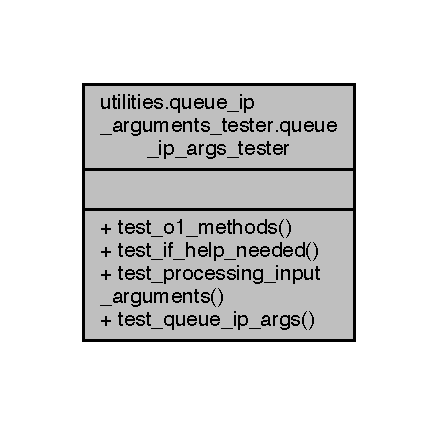
\includegraphics[width=210pt]{d0/dd1/classutilities_1_1queue__ip__arguments__tester_1_1queue__ip__args__tester__coll__graph}
\end{center}
\end{figure}
\subsection*{Static Public Member Functions}
\begin{DoxyCompactItemize}
\item 
def \hyperlink{classutilities_1_1queue__ip__arguments__tester_1_1queue__ip__args__tester_a49bd049dbf616cc1f604d3c0cbe84c43}{test\+\_\+o1\+\_\+methods} ()
\begin{DoxyCompactList}\small\item\em ========================================================= Method to test the O(1) methods that print information to the standard output, or are accessor methods. \end{DoxyCompactList}\item 
def \hyperlink{classutilities_1_1queue__ip__arguments__tester_1_1queue__ip__args__tester_a4af9d2177916d79d95fc9de5531162af}{test\+\_\+if\+\_\+help\+\_\+needed} ()
\begin{DoxyCompactList}\small\item\em ========================================================= Method to test if the user wants to read the brief user manual. \end{DoxyCompactList}\item 
def \hyperlink{classutilities_1_1queue__ip__arguments__tester_1_1queue__ip__args__tester_a53e53ec2797918a6488b0d75ba437407}{test\+\_\+processing\+\_\+input\+\_\+arguments} ()
\begin{DoxyCompactList}\small\item\em ========================================================= Method to test the processing of the 1st \& 2nd input arguments. \end{DoxyCompactList}\item 
def \hyperlink{classutilities_1_1queue__ip__arguments__tester_1_1queue__ip__args__tester_aee90077323d94238d7f81b23e31207c3}{test\+\_\+queue\+\_\+ip\+\_\+args} ()
\begin{DoxyCompactList}\small\item\em ========================================================= Method to test methods that process input arguments to the software. \end{DoxyCompactList}\end{DoxyCompactItemize}


\subsection{Detailed Description}


Definition at line \hyperlink{queue__ip__arguments__tester_8py_source_l00093}{93} of file \hyperlink{queue__ip__arguments__tester_8py_source}{queue\+\_\+ip\+\_\+arguments\+\_\+tester.\+py}.



\subsection{Member Function Documentation}
\hypertarget{classutilities_1_1queue__ip__arguments__tester_1_1queue__ip__args__tester_a4af9d2177916d79d95fc9de5531162af}{}\index{utilities\+::queue\+\_\+ip\+\_\+arguments\+\_\+tester\+::queue\+\_\+ip\+\_\+args\+\_\+tester@{utilities\+::queue\+\_\+ip\+\_\+arguments\+\_\+tester\+::queue\+\_\+ip\+\_\+args\+\_\+tester}!test\+\_\+if\+\_\+help\+\_\+needed@{test\+\_\+if\+\_\+help\+\_\+needed}}
\index{test\+\_\+if\+\_\+help\+\_\+needed@{test\+\_\+if\+\_\+help\+\_\+needed}!utilities\+::queue\+\_\+ip\+\_\+arguments\+\_\+tester\+::queue\+\_\+ip\+\_\+args\+\_\+tester@{utilities\+::queue\+\_\+ip\+\_\+arguments\+\_\+tester\+::queue\+\_\+ip\+\_\+args\+\_\+tester}}
\subsubsection[{test\+\_\+if\+\_\+help\+\_\+needed()}]{\setlength{\rightskip}{0pt plus 5cm}def utilities.\+queue\+\_\+ip\+\_\+arguments\+\_\+tester.\+queue\+\_\+ip\+\_\+args\+\_\+tester.\+test\+\_\+if\+\_\+help\+\_\+needed (
\begin{DoxyParamCaption}
{}
\end{DoxyParamCaption}
)\hspace{0.3cm}{\ttfamily [static]}}\label{classutilities_1_1queue__ip__arguments__tester_1_1queue__ip__args__tester_a4af9d2177916d79d95fc9de5531162af}


========================================================= Method to test if the user wants to read the brief user manual. 

\begin{DoxyReturn}{Returns}
-\/ Nothing. O(1) method. 
\end{DoxyReturn}


Definition at line \hyperlink{queue__ip__arguments__tester_8py_source_l00264}{264} of file \hyperlink{queue__ip__arguments__tester_8py_source}{queue\+\_\+ip\+\_\+arguments\+\_\+tester.\+py}.


\begin{DoxyCode}
\hypertarget{classutilities_1_1queue__ip__arguments__tester_1_1queue__ip__args__tester_l00264}{}\hyperlink{classutilities_1_1queue__ip__arguments__tester_1_1queue__ip__args__tester_a4af9d2177916d79d95fc9de5531162af}{00264}     \textcolor{keyword}{def }\hyperlink{classutilities_1_1queue__ip__arguments__tester_1_1queue__ip__args__tester_a4af9d2177916d79d95fc9de5531162af}{test\_if\_help\_needed}():
00265         print(\textcolor{stringliteral}{" Testing for no help needed..."})
00266         \textcolor{comment}{#   Set the list of input arguments to have 2 arguments.}
00267         name\_of\_script\_dumped = \textcolor{stringliteral}{"name-of-the-script"}
00268         current\_1st\_ip\_arg = \textcolor{stringliteral}{"garbage.json"}
00269         current\_2nd\_ip\_arg = \textcolor{stringliteral}{"nonsense.json"}
00270         new\_list\_ip\_args = [name\_of\_script\_dumped, current\_1st\_ip\_arg, current\_2nd\_ip\_arg]
00271         \textcolor{comment}{#   Assign input arguments to "set\_input\_arguments(...)" for processing.}
00272         queue\_ip\_args.set\_input\_arguments(new\_list\_ip\_args)
00273         prompt8 = \textcolor{stringliteral}{" ... Test: queue\_ip\_args.check\_if\_help\_wanted()  \{\}"}
00274         statistical\_analysis.increment\_number\_test\_cases\_used()
00275         queue\_ip\_args.check\_if\_help\_wanted()
00276         print(prompt8 .format(\textcolor{stringliteral}{" OK"}))
00277         statistical\_analysis.increment\_number\_test\_cases\_passed()
00278         print(\textcolor{stringliteral}{" Testing for help needed (1st arg)... "})
00279         \textcolor{comment}{#   Change the list of input arguments to have "-h" option.}
00280         current\_1st\_ip\_arg = \textcolor{stringliteral}{"-h"}
00281         new\_list\_ip\_args = [name\_of\_script\_dumped, current\_1st\_ip\_arg, current\_2nd\_ip\_arg]
00282         \textcolor{comment}{#   Assign input arguments to "set\_input\_arguments(...)" for processing.}
00283         queue\_ip\_args.set\_input\_arguments(new\_list\_ip\_args)
00284         statistical\_analysis.increment\_number\_test\_cases\_used()
00285         \textcolor{keywordflow}{try}:
00286             queue\_ip\_args.check\_if\_help\_wanted()
00287             print(prompt8 .format(\textcolor{stringliteral}{"FAIL!!!"}))
00288         \textcolor{keywordflow}{except}:
00289             print(prompt8 .format(\textcolor{stringliteral}{" OK"}))
00290             statistical\_analysis.increment\_number\_test\_cases\_passed()
00291         print(\textcolor{stringliteral}{" Testing for help needed (2nd arg)... "})
00292         current\_1st\_ip\_arg = \textcolor{stringliteral}{"garbage.json"}
00293         current\_2nd\_ip\_arg = \textcolor{stringliteral}{"-h"}
00294         new\_list\_ip\_args = [name\_of\_script\_dumped, current\_1st\_ip\_arg, current\_2nd\_ip\_arg]
00295         \textcolor{comment}{#   Assign input arguments to "set\_input\_arguments(...)" for processing.}
00296         queue\_ip\_args.set\_input\_arguments(new\_list\_ip\_args)
00297         statistical\_analysis.increment\_number\_test\_cases\_used()
00298         \textcolor{keywordflow}{try}:
00299             queue\_ip\_args.check\_if\_help\_wanted()
00300             print(prompt8 .format(\textcolor{stringliteral}{"FAIL!!!"}))
00301         \textcolor{keywordflow}{except}:
00302             print(prompt8 .format(\textcolor{stringliteral}{" OK"}))
00303             statistical\_analysis.increment\_number\_test\_cases\_passed()
00304         print(\textcolor{stringliteral}{" Testing for help needed (3rd arg)... "})
00305         current\_1st\_ip\_arg = \textcolor{stringliteral}{"garbage.json"}
00306         current\_2nd\_ip\_arg = \textcolor{stringliteral}{"nonsense.json"}
00307         current\_3rd\_ip\_arg = \textcolor{stringliteral}{"-h"}
00308         new\_list\_ip\_args = [name\_of\_script\_dumped, current\_1st\_ip\_arg, current\_2nd\_ip\_arg, 
      current\_3rd\_ip\_arg]
00309         \textcolor{comment}{#   Assign input arguments to "set\_input\_arguments(...)" for processing.}
00310         queue\_ip\_args.set\_input\_arguments(new\_list\_ip\_args)
00311         statistical\_analysis.increment\_number\_test\_cases\_used()
00312         \textcolor{keywordflow}{try}:
00313             queue\_ip\_args.check\_if\_help\_wanted()
00314             print(prompt8 .format(\textcolor{stringliteral}{"FAIL!!!"}))
00315         \textcolor{keywordflow}{except}:
00316             print(prompt8 .format(\textcolor{stringliteral}{" OK"}))
00317             statistical\_analysis.increment\_number\_test\_cases\_passed()
\end{DoxyCode}
\hypertarget{classutilities_1_1queue__ip__arguments__tester_1_1queue__ip__args__tester_a49bd049dbf616cc1f604d3c0cbe84c43}{}\index{utilities\+::queue\+\_\+ip\+\_\+arguments\+\_\+tester\+::queue\+\_\+ip\+\_\+args\+\_\+tester@{utilities\+::queue\+\_\+ip\+\_\+arguments\+\_\+tester\+::queue\+\_\+ip\+\_\+args\+\_\+tester}!test\+\_\+o1\+\_\+methods@{test\+\_\+o1\+\_\+methods}}
\index{test\+\_\+o1\+\_\+methods@{test\+\_\+o1\+\_\+methods}!utilities\+::queue\+\_\+ip\+\_\+arguments\+\_\+tester\+::queue\+\_\+ip\+\_\+args\+\_\+tester@{utilities\+::queue\+\_\+ip\+\_\+arguments\+\_\+tester\+::queue\+\_\+ip\+\_\+args\+\_\+tester}}
\subsubsection[{test\+\_\+o1\+\_\+methods()}]{\setlength{\rightskip}{0pt plus 5cm}def utilities.\+queue\+\_\+ip\+\_\+arguments\+\_\+tester.\+queue\+\_\+ip\+\_\+args\+\_\+tester.\+test\+\_\+o1\+\_\+methods (
\begin{DoxyParamCaption}
{}
\end{DoxyParamCaption}
)\hspace{0.3cm}{\ttfamily [static]}}\label{classutilities_1_1queue__ip__arguments__tester_1_1queue__ip__args__tester_a49bd049dbf616cc1f604d3c0cbe84c43}


========================================================= Method to test the O(1) methods that print information to the standard output, or are accessor methods. 

\begin{DoxyReturn}{Returns}
-\/ Nothing. O(1) method. O(n) in terms of the number of input arguments. 
\end{DoxyReturn}


Definition at line \hyperlink{queue__ip__arguments__tester_8py_source_l00101}{101} of file \hyperlink{queue__ip__arguments__tester_8py_source}{queue\+\_\+ip\+\_\+arguments\+\_\+tester.\+py}.


\begin{DoxyCode}
\hypertarget{classutilities_1_1queue__ip__arguments__tester_1_1queue__ip__args__tester_l00101}{}\hyperlink{classutilities_1_1queue__ip__arguments__tester_1_1queue__ip__args__tester_a49bd049dbf616cc1f604d3c0cbe84c43}{00101}     \textcolor{keyword}{def }\hyperlink{classutilities_1_1queue__ip__arguments__tester_1_1queue__ip__args__tester_a49bd049dbf616cc1f604d3c0cbe84c43}{test\_o1\_methods}():
00102         print(\textcolor{stringliteral}{" Test: queue\_ip\_args.how\_to\_use\_script()         OK"})
00103         queue\_ip\_args.how\_to\_use\_script()
00104         statistical\_analysis.increment\_number\_test\_cases\_used()
00105         statistical\_analysis.increment\_number\_test\_cases\_passed()
00106         print(\textcolor{stringliteral}{" Test: queue\_ip\_args.print\_help\_option()         OK"})
00107         queue\_ip\_args.print\_help\_option()
00108         statistical\_analysis.increment\_number\_test\_cases\_used()
00109         statistical\_analysis.increment\_number\_test\_cases\_passed()
00110         print(\textcolor{stringliteral}{" Test: queue\_ip\_args.get\_list\_of\_input\_arguments()   OK"})
00111         temp\_set\_ip\_args = queue\_ip\_args.get\_list\_of\_input\_arguments()
00112         statistical\_analysis.increment\_number\_test\_cases\_used()
00113         statistical\_analysis.increment\_number\_test\_cases\_passed()
00114         \textcolor{comment}{#   -   -   -   -   -   -   -   -   -   -   -   -   -   -   -}
00115         print(\textcolor{stringliteral}{" Test: queue\_ip\_args.print\_all\_input\_arguments()     OK"})
00116         queue\_ip\_args.print\_all\_input\_arguments()
00117         statistical\_analysis.increment\_number\_test\_cases\_used()
00118         statistical\_analysis.increment\_number\_test\_cases\_passed()
00119         \textcolor{comment}{#   -   -   -   -   -   -   -   -   -   -   -   -   -   -   -}
00120         prompt = \textcolor{stringliteral}{"  Test: queue\_ip\_args.get\_1st\_input\_argument()        \{\}"}
00121         statistical\_analysis.increment\_number\_test\_cases\_used()
00122         \textcolor{keywordflow}{if} queue\_ip\_args.get\_1st\_input\_argument() \textcolor{keywordflow}{is} \textcolor{keywordflow}{not} \textcolor{keywordtype}{None}:
00123             print(prompt .format(\textcolor{stringliteral}{"OK"}))
00124             statistical\_analysis.increment\_number\_test\_cases\_passed()
00125         \textcolor{keywordflow}{else}:
00126             print(prompt .format(\textcolor{stringliteral}{"FAIL!!!"}))
00127         \textcolor{comment}{#   -   -   -   -   -   -   -   -   -   -   -   -   -   -   -}
00128         prompt = \textcolor{stringliteral}{"  Test: queue\_ip\_args.get\_2nd\_input\_argument()        \{\}"}
00129         statistical\_analysis.increment\_number\_test\_cases\_used()
00130         \textcolor{keywordflow}{if} queue\_ip\_args.get\_2nd\_input\_argument() \textcolor{keywordflow}{is} \textcolor{keywordflow}{not} \textcolor{keywordtype}{None}:
00131             print(prompt .format(\textcolor{stringliteral}{"OK"}))
00132             statistical\_analysis.increment\_number\_test\_cases\_passed()
00133         \textcolor{keywordflow}{else}:
00134             print(prompt .format(\textcolor{stringliteral}{"FAIL!!!"}))
00135         \textcolor{comment}{#   -   -   -   -   -   -   -   -   -   -   -   -   -   -   -}
00136         print(\textcolor{stringliteral}{" Testing for an empty list..."})
00137         prompt1 = \textcolor{stringliteral}{" ... Test: queue\_ip\_args.get\_list\_of\_input\_arguments()   \{\}"}
00138         statistical\_analysis.increment\_number\_test\_cases\_used()
00139         prompt2 = \textcolor{stringliteral}{" ... Test: queue\_ip\_args.get\_number\_of\_input\_arguments() \{\}"}
00140         statistical\_analysis.increment\_number\_test\_cases\_used()
00141         prompt4 = \textcolor{stringliteral}{" ... Test: queue\_ip\_args.set\_input\_arguments(...)    \{\}"}
00142         statistical\_analysis.increment\_number\_test\_cases\_used()
00143         prompt5 = \textcolor{stringliteral}{" ... Test: queue\_ip\_args.get\_1st\_input\_argument()    \{\}"}
00144         prompt6 = \textcolor{stringliteral}{" ... Test: queue\_ip\_args.get\_2nd\_input\_argument()    \{\}"}
00145         \textcolor{comment}{#   List of input arguments.}
00146         old\_list\_ip\_args = queue\_ip\_args.get\_list\_of\_input\_arguments()
00147         new\_list\_ip\_args = []
00148         \textcolor{stringliteral}{"""}
00149 \textcolor{stringliteral}{            Assign input arguments to "set\_input\_arguments(...)" for}
00150 \textcolor{stringliteral}{                processing.}
00151 \textcolor{stringliteral}{            Statement should fail.}
00152 \textcolor{stringliteral}{        """}
00153         \textcolor{keywordflow}{try}:
00154             queue\_ip\_args.set\_input\_arguments(new\_list\_ip\_args)
00155         \textcolor{keywordflow}{except}:
00156             \textcolor{keywordflow}{if} old\_list\_ip\_args == queue\_ip\_args.get\_list\_of\_input\_arguments():
00157                 print(prompt1 .format(\textcolor{stringliteral}{"OK"}))
00158                 statistical\_analysis.increment\_number\_test\_cases\_passed()
00159             \textcolor{keywordflow}{else}:
00160                 print(prompt1 .format(\textcolor{stringliteral}{"FAIL!!!"}))
00161                 \textcolor{comment}{#print(queue\_ip\_args.get\_list\_of\_input\_arguments())}
00162             \textcolor{keywordflow}{if} len(old\_list\_ip\_args) == queue\_ip\_args.get\_number\_of\_input\_arguments():
00163                 print(prompt2 .format(\textcolor{stringliteral}{"OK"}))
00164                 statistical\_analysis.increment\_number\_test\_cases\_passed()
00165             \textcolor{keywordflow}{else}:
00166                 print(prompt2 .format(\textcolor{stringliteral}{"FAIL!!!"}))
00167                 \textcolor{comment}{#print(queue\_ip\_args.get\_number\_of\_input\_arguments())}
00168             print(prompt4 .format(\textcolor{stringliteral}{"OK"}))
00169             statistical\_analysis.increment\_number\_test\_cases\_passed()
00170         print(\textcolor{stringliteral}{" Testing for list with 1 argument..."})
00171         \textcolor{stringliteral}{"""}
00172 \textcolor{stringliteral}{            Set the list of input arguments to have 1 argument, in addition}
00173 \textcolor{stringliteral}{                to the name of the script.}
00174 \textcolor{stringliteral}{            Hence, the list would have 2 arguments, since the first}
00175 \textcolor{stringliteral}{                "argument" is dumped during the method call to}
00176 \textcolor{stringliteral}{                set\_input\_arguments(...);}
00177 \textcolor{stringliteral}{                this first "argument" is the name of the currently executing}
00178 \textcolor{stringliteral}{                    script.}
00179 \textcolor{stringliteral}{        """}
00180         name\_of\_script\_dumped = \textcolor{stringliteral}{"name-of-the-script"}
00181         current\_1st\_ip\_arg = \textcolor{stringliteral}{"benchmarks/majority\_netlist.json"}
00182         new\_list\_ip\_args = [name\_of\_script\_dumped, current\_1st\_ip\_arg]
00183         \textcolor{comment}{#   Assign input arguments to "set\_input\_arguments(...)" for processing.}
00184         queue\_ip\_args.set\_input\_arguments(new\_list\_ip\_args)
00185         statistical\_analysis.increment\_number\_test\_cases\_used()
00186         \textcolor{keywordflow}{if} new\_list\_ip\_args == queue\_ip\_args.get\_list\_of\_input\_arguments():
00187             print(prompt1 .format(\textcolor{stringliteral}{"OK"}))
00188             statistical\_analysis.increment\_number\_test\_cases\_passed()
00189         \textcolor{keywordflow}{else}:
00190             print(prompt1 .format(\textcolor{stringliteral}{"FAIL!!!"}))
00191             \textcolor{comment}{#print(queue\_ip\_args.get\_list\_of\_input\_arguments())}
00192         statistical\_analysis.increment\_number\_test\_cases\_used()
00193         \textcolor{keywordflow}{if} len(new\_list\_ip\_args) == queue\_ip\_args.get\_number\_of\_input\_arguments():
00194             print(prompt2 .format(\textcolor{stringliteral}{"OK"}))
00195             statistical\_analysis.increment\_number\_test\_cases\_passed()
00196         \textcolor{keywordflow}{else}:
00197             print(prompt2 .format(\textcolor{stringliteral}{"FAIL!!!"}))
00198             \textcolor{comment}{#print(len(new\_list\_ip\_args)-1)}
00199             \textcolor{comment}{#print(queue\_ip\_args.get\_number\_of\_input\_arguments())}
00200         statistical\_analysis.increment\_number\_test\_cases\_used()
00201         print(prompt4 .format(\textcolor{stringliteral}{"OK"}))
00202         statistical\_analysis.increment\_number\_test\_cases\_passed()
00203         \textcolor{comment}{#   -   -   -   -   -   -   -   -   -   -   -   -   -   -}
00204         statistical\_analysis.increment\_number\_test\_cases\_used()
00205         \textcolor{keywordflow}{if} current\_1st\_ip\_arg == queue\_ip\_args.get\_1st\_input\_argument():
00206             print(prompt5 .format(\textcolor{stringliteral}{"OK"}))
00207             statistical\_analysis.increment\_number\_test\_cases\_passed()
00208         \textcolor{keywordflow}{else}:
00209             print(prompt5 .format(\textcolor{stringliteral}{"FAIL!!!"}))
00210         \textcolor{stringliteral}{"""}
00211 \textcolor{stringliteral}{            If an input argument for the software is "-h", show the}
00212 \textcolor{stringliteral}{                brief user manual to the user.}
00213 \textcolor{stringliteral}{            Else, there is no need to test for more than 2 input arguments}
00214 \textcolor{stringliteral}{                for the software, since only the first two are processed.}
00215 \textcolor{stringliteral}{            So, the list shall have 3 elements, since the first element}
00216 \textcolor{stringliteral}{                is dumped during the method call to set\_input\_arguments(...).}
00217 \textcolor{stringliteral}{        """}
00218         print(\textcolor{stringliteral}{" Testing for list with 2 arguments..."})
00219         \textcolor{comment}{#   Set the list of input arguments to have 2 arguments.}
00220         \textcolor{comment}{#new\_list\_ip\_args = ["benchmarks/majority\_netlist.json" "nonsense.json"]}
00221         current\_1st\_ip\_arg = \textcolor{stringliteral}{"garbage.json"}
00222         current\_2nd\_ip\_arg = \textcolor{stringliteral}{"nonsense.json"}
00223         new\_list\_ip\_args = [name\_of\_script\_dumped, current\_1st\_ip\_arg, current\_2nd\_ip\_arg]
00224         \textcolor{comment}{#   Assign input arguments to "set\_input\_arguments(...)" for processing.}
00225         queue\_ip\_args.set\_input\_arguments(new\_list\_ip\_args)
00226         statistical\_analysis.increment\_number\_test\_cases\_used()
00227         \textcolor{keywordflow}{if} new\_list\_ip\_args == queue\_ip\_args.get\_list\_of\_input\_arguments():
00228             print(prompt1 .format(\textcolor{stringliteral}{"OK"}))
00229             statistical\_analysis.increment\_number\_test\_cases\_passed()
00230         \textcolor{keywordflow}{else}:
00231             print(prompt1 .format(\textcolor{stringliteral}{"FAIL!!!"}))
00232             \textcolor{comment}{#print(queue\_ip\_args.get\_list\_of\_input\_arguments())}
00233         statistical\_analysis.increment\_number\_test\_cases\_used()
00234         \textcolor{keywordflow}{if} len(new\_list\_ip\_args) == queue\_ip\_args.get\_number\_of\_input\_arguments():
00235             print(prompt2 .format(\textcolor{stringliteral}{"OK"}))
00236             statistical\_analysis.increment\_number\_test\_cases\_passed()
00237         \textcolor{keywordflow}{else}:
00238             print(prompt2 .format(\textcolor{stringliteral}{"FAIL!!!"}))
00239             \textcolor{comment}{#print(queue\_ip\_args.get\_number\_of\_input\_arguments())}
00240         statistical\_analysis.increment\_number\_test\_cases\_used()
00241         print(prompt4 .format(\textcolor{stringliteral}{"OK"}))
00242         statistical\_analysis.increment\_number\_test\_cases\_passed()
00243         \textcolor{comment}{#   -   -   -   -   -   -   -   -   -   -   -   -   -   -}
00244         statistical\_analysis.increment\_number\_test\_cases\_used()
00245         \textcolor{keywordflow}{if} current\_2nd\_ip\_arg == queue\_ip\_args.get\_2nd\_input\_argument():
00246             print(prompt6 .format(\textcolor{stringliteral}{"OK"}))
00247             statistical\_analysis.increment\_number\_test\_cases\_passed()
00248         \textcolor{keywordflow}{else}:
00249             print(prompt6 .format(\textcolor{stringliteral}{"FAIL!!!"}))
00250         prompt7 = \textcolor{stringliteral}{" ... Test: queue\_ip\_args.input\_arguments\_error() \{\}"}
00251         statistical\_analysis.increment\_number\_test\_cases\_used()
00252         \textcolor{keywordflow}{try}:
00253             queue\_ip\_args.input\_arguments\_error()
00254             print(prompt7 .format(\textcolor{stringliteral}{"FAIL!!!"}))
00255         \textcolor{keywordflow}{except}:
00256             print(prompt7 .format(\textcolor{stringliteral}{" OK"}))
00257             statistical\_analysis.increment\_number\_test\_cases\_passed()
\end{DoxyCode}
\hypertarget{classutilities_1_1queue__ip__arguments__tester_1_1queue__ip__args__tester_a53e53ec2797918a6488b0d75ba437407}{}\index{utilities\+::queue\+\_\+ip\+\_\+arguments\+\_\+tester\+::queue\+\_\+ip\+\_\+args\+\_\+tester@{utilities\+::queue\+\_\+ip\+\_\+arguments\+\_\+tester\+::queue\+\_\+ip\+\_\+args\+\_\+tester}!test\+\_\+processing\+\_\+input\+\_\+arguments@{test\+\_\+processing\+\_\+input\+\_\+arguments}}
\index{test\+\_\+processing\+\_\+input\+\_\+arguments@{test\+\_\+processing\+\_\+input\+\_\+arguments}!utilities\+::queue\+\_\+ip\+\_\+arguments\+\_\+tester\+::queue\+\_\+ip\+\_\+args\+\_\+tester@{utilities\+::queue\+\_\+ip\+\_\+arguments\+\_\+tester\+::queue\+\_\+ip\+\_\+args\+\_\+tester}}
\subsubsection[{test\+\_\+processing\+\_\+input\+\_\+arguments()}]{\setlength{\rightskip}{0pt plus 5cm}def utilities.\+queue\+\_\+ip\+\_\+arguments\+\_\+tester.\+queue\+\_\+ip\+\_\+args\+\_\+tester.\+test\+\_\+processing\+\_\+input\+\_\+arguments (
\begin{DoxyParamCaption}
{}
\end{DoxyParamCaption}
)\hspace{0.3cm}{\ttfamily [static]}}\label{classutilities_1_1queue__ip__arguments__tester_1_1queue__ip__args__tester_a53e53ec2797918a6488b0d75ba437407}


========================================================= Method to test the processing of the 1st \& 2nd input arguments. 

\begin{DoxyReturn}{Returns}
-\/ Nothing. O(1) method. 
\end{DoxyReturn}


Definition at line \hyperlink{queue__ip__arguments__tester_8py_source_l00323}{323} of file \hyperlink{queue__ip__arguments__tester_8py_source}{queue\+\_\+ip\+\_\+arguments\+\_\+tester.\+py}.


\begin{DoxyCode}
\hypertarget{classutilities_1_1queue__ip__arguments__tester_1_1queue__ip__args__tester_l00323}{}\hyperlink{classutilities_1_1queue__ip__arguments__tester_1_1queue__ip__args__tester_a53e53ec2797918a6488b0d75ba437407}{00323}     \textcolor{keyword}{def }\hyperlink{classutilities_1_1queue__ip__arguments__tester_1_1queue__ip__args__tester_a53e53ec2797918a6488b0d75ba437407}{test\_processing\_input\_arguments}():
00324         print(\textcolor{stringliteral}{" Test: queue\_ip\_args.process\_1st\_ip\_arg()... "})
00325         name\_of\_script\_dumped = \textcolor{stringliteral}{"name-of-the-script"}
00326         current\_1st\_ip\_arg = \textcolor{stringliteral}{"garbage.json"}
00327         current\_2nd\_ip\_arg = \textcolor{stringliteral}{"notes/guidelines/guidelines.tex"}
00328         new\_list\_ip\_args = [name\_of\_script\_dumped, current\_1st\_ip\_arg, current\_2nd\_ip\_arg]
00329         \textcolor{comment}{#   Assign input arguments to "set\_input\_arguments(...)" for processing.}
00330         queue\_ip\_args.set\_input\_arguments(new\_list\_ip\_args)
00331         prompt9 = \textcolor{stringliteral}{" ... Invalid path to file    \{\}"}
00332         statistical\_analysis.increment\_number\_test\_cases\_used()
00333         \textcolor{keywordflow}{try}:
00334             ip\_fname = queue\_ip\_args.process\_1st\_ip\_arg()
00335             print(prompt9 .format(\textcolor{stringliteral}{"     FAIL!!!"}))
00336         \textcolor{keywordflow}{except}:
00337             print(prompt9 .format(\textcolor{stringliteral}{"         OK"}))
00338             statistical\_analysis.increment\_number\_test\_cases\_passed()
00339         \textcolor{comment}{#   -   -   -   -   -   -   -   -   -   -   -   -   -}
00340         \textcolor{stringliteral}{"""}
00341 \textcolor{stringliteral}{            1st input argument: Valid path to file, no JSON file extension.}
00342 \textcolor{stringliteral}{        """}
00343         \textcolor{comment}{#current\_1st\_ip\_arg = "benchmarks/majority\_netlist.json"}
00344         current\_1st\_ip\_arg = \textcolor{stringliteral}{"notes/mit-license.text"}
00345         new\_list\_ip\_args = [name\_of\_script\_dumped, current\_1st\_ip\_arg, current\_2nd\_ip\_arg]
00346         queue\_ip\_args.set\_input\_arguments(new\_list\_ip\_args)
00347         prompt10 = \textcolor{stringliteral}{"    ... Valid path to file, no JSON file extension. \{\}"}
00348         statistical\_analysis.increment\_number\_test\_cases\_used()
00349         \textcolor{keywordflow}{try}:
00350             ip\_fname = queue\_ip\_args.process\_1st\_ip\_arg()
00351             print(prompt10 .format(\textcolor{stringliteral}{"        FAIL!!!"}))
00352         \textcolor{keywordflow}{except}:
00353             print(prompt10 .format(\textcolor{stringliteral}{"    OK"}))
00354             statistical\_analysis.increment\_number\_test\_cases\_passed()
00355         \textcolor{stringliteral}{"""}
00356 \textcolor{stringliteral}{            1st input argument: Valid path to file, JSON file extension.}
00357 \textcolor{stringliteral}{        """}
00358         current\_1st\_ip\_arg = \textcolor{stringliteral}{"benchmarks/majority\_netlist.json"}
00359         new\_list\_ip\_args = [name\_of\_script\_dumped, current\_1st\_ip\_arg, current\_2nd\_ip\_arg]
00360         queue\_ip\_args.set\_input\_arguments(new\_list\_ip\_args)
00361         prompt10 = \textcolor{stringliteral}{"    ... Valid path to file, JSON file extension.    \{\}"}
00362         statistical\_analysis.increment\_number\_test\_cases\_used()
00363         ip\_fname = queue\_ip\_args.process\_1st\_ip\_arg()
00364         print(prompt10 .format(\textcolor{stringliteral}{"    OK"}))
00365         statistical\_analysis.increment\_number\_test\_cases\_passed()
00366         print(\textcolor{stringliteral}{" -   -   -   -   -   -   -   -"})
00367         print(\textcolor{stringliteral}{" Test: queue\_ip\_args.process\_2nd\_ip\_arg()... "})
00368         prompt11 = \textcolor{stringliteral}{"    ... Valid path to file  \{\}"}
00369         statistical\_analysis.increment\_number\_test\_cases\_used()
00370         \textcolor{keywordflow}{try}:
00371             op\_fname = queue\_ip\_args.process\_2nd\_ip\_arg()
00372             print(prompt11 .format(\textcolor{stringliteral}{"                FAIL!!!"}))
00373         \textcolor{keywordflow}{except}:
00374             print(prompt11 .format(\textcolor{stringliteral}{"                OK"}))
00375             statistical\_analysis.increment\_number\_test\_cases\_passed()
00376         prompt12 = \textcolor{stringliteral}{"    ... Invalid path to file, no JSON extension \{\}"}
00377         statistical\_analysis.increment\_number\_test\_cases\_used()
00378         current\_2nd\_ip\_arg = \textcolor{stringliteral}{"nonsense"}
00379         new\_list\_ip\_args = [name\_of\_script\_dumped, current\_1st\_ip\_arg, current\_2nd\_ip\_arg]
00380         queue\_ip\_args.set\_input\_arguments(new\_list\_ip\_args)
00381         \textcolor{keywordflow}{try}:
00382             op\_fname = queue\_ip\_args.process\_2nd\_ip\_arg()
00383             print(prompt12 .format(\textcolor{stringliteral}{"    OK"}))
00384             statistical\_analysis.increment\_number\_test\_cases\_passed()
00385         \textcolor{keywordflow}{except}:
00386             print(prompt12 .format(\textcolor{stringliteral}{"    FAIL!!!"}))
00387         prompt13 = \textcolor{stringliteral}{"    ... Invalid path to file, JSON extension    \{\}"}
00388         statistical\_analysis.increment\_number\_test\_cases\_used()
00389         current\_2nd\_ip\_arg = \textcolor{stringliteral}{"nonsense.json"}
00390         new\_list\_ip\_args = [name\_of\_script\_dumped, current\_1st\_ip\_arg, current\_2nd\_ip\_arg]
00391         queue\_ip\_args.set\_input\_arguments(new\_list\_ip\_args)
00392         \textcolor{keywordflow}{try}:
00393             op\_fname = queue\_ip\_args.process\_2nd\_ip\_arg()
00394             print(prompt13 .format(\textcolor{stringliteral}{"    OK"}))
00395             statistical\_analysis.increment\_number\_test\_cases\_passed()
00396         \textcolor{keywordflow}{except}:
00397             print(prompt13 .format(\textcolor{stringliteral}{"    FAIL!!!"}))
00398 
\end{DoxyCode}
\hypertarget{classutilities_1_1queue__ip__arguments__tester_1_1queue__ip__args__tester_aee90077323d94238d7f81b23e31207c3}{}\index{utilities\+::queue\+\_\+ip\+\_\+arguments\+\_\+tester\+::queue\+\_\+ip\+\_\+args\+\_\+tester@{utilities\+::queue\+\_\+ip\+\_\+arguments\+\_\+tester\+::queue\+\_\+ip\+\_\+args\+\_\+tester}!test\+\_\+queue\+\_\+ip\+\_\+args@{test\+\_\+queue\+\_\+ip\+\_\+args}}
\index{test\+\_\+queue\+\_\+ip\+\_\+args@{test\+\_\+queue\+\_\+ip\+\_\+args}!utilities\+::queue\+\_\+ip\+\_\+arguments\+\_\+tester\+::queue\+\_\+ip\+\_\+args\+\_\+tester@{utilities\+::queue\+\_\+ip\+\_\+arguments\+\_\+tester\+::queue\+\_\+ip\+\_\+args\+\_\+tester}}
\subsubsection[{test\+\_\+queue\+\_\+ip\+\_\+args()}]{\setlength{\rightskip}{0pt plus 5cm}def utilities.\+queue\+\_\+ip\+\_\+arguments\+\_\+tester.\+queue\+\_\+ip\+\_\+args\+\_\+tester.\+test\+\_\+queue\+\_\+ip\+\_\+args (
\begin{DoxyParamCaption}
{}
\end{DoxyParamCaption}
)\hspace{0.3cm}{\ttfamily [static]}}\label{classutilities_1_1queue__ip__arguments__tester_1_1queue__ip__args__tester_aee90077323d94238d7f81b23e31207c3}


========================================================= Method to test methods that process input arguments to the software. 

\begin{DoxyReturn}{Returns}
-\/ Nothing. O(1) method. 
\end{DoxyReturn}


Definition at line \hyperlink{queue__ip__arguments__tester_8py_source_l00405}{405} of file \hyperlink{queue__ip__arguments__tester_8py_source}{queue\+\_\+ip\+\_\+arguments\+\_\+tester.\+py}.


\begin{DoxyCode}
\hypertarget{classutilities_1_1queue__ip__arguments__tester_1_1queue__ip__args__tester_l00405}{}\hyperlink{classutilities_1_1queue__ip__arguments__tester_1_1queue__ip__args__tester_aee90077323d94238d7f81b23e31207c3}{00405}     \textcolor{keyword}{def }\hyperlink{classutilities_1_1queue__ip__arguments__tester_1_1queue__ip__args__tester_aee90077323d94238d7f81b23e31207c3}{test\_queue\_ip\_args}():
00406         print(\textcolor{stringliteral}{""})
00407         print(\textcolor{stringliteral}{""})
00408         print(\textcolor{stringliteral}{"==   Testing class: queue\_ip\_args."})
00409         queue\_ip\_args\_tester.test\_o1\_methods()
00410         queue\_ip\_args\_tester.test\_if\_help\_needed()
00411         queue\_ip\_args\_tester.test\_processing\_input\_arguments()
00412 \end{DoxyCode}


The documentation for this class was generated from the following file\+:\begin{DoxyCompactItemize}
\item 
utilities/\hyperlink{queue__ip__arguments__tester_8py}{queue\+\_\+ip\+\_\+arguments\+\_\+tester.\+py}\end{DoxyCompactItemize}

\hypertarget{classrandom__process__models_1_1random__process__generator_1_1rand__signal__generator}{}\section{random\+\_\+process\+\_\+models.\+random\+\_\+process\+\_\+generator.\+rand\+\_\+signal\+\_\+generator Class Reference}
\label{classrandom__process__models_1_1random__process__generator_1_1rand__signal__generator}\index{random\+\_\+process\+\_\+models.\+random\+\_\+process\+\_\+generator.\+rand\+\_\+signal\+\_\+generator@{random\+\_\+process\+\_\+models.\+random\+\_\+process\+\_\+generator.\+rand\+\_\+signal\+\_\+generator}}


Collaboration diagram for random\+\_\+process\+\_\+models.\+random\+\_\+process\+\_\+generator.\+rand\+\_\+signal\+\_\+generator\+:
\nopagebreak
\begin{figure}[H]
\begin{center}
\leavevmode

\includegraphics[width=244pt]{d8/df9/classrandom__process__models_1_1random__process__generator_1_1rand__signal__generator__coll__graph}
\end{center}
\end{figure}
\subsection*{Static Public Member Functions}
\begin{DoxyCompactItemize}
\item 
def \hyperlink{classrandom__process__models_1_1random__process__generator_1_1rand__signal__generator_a0120f8a5803679907bca0d8267e30781}{gen\+\_\+rand\+\_\+signal\+\_\+uniform\+\_\+distributn}
\begin{DoxyCompactList}\small\item\em Method to generate a discrete-\/time random signal/process for \char`\"{}n\char`\"{} values. \end{DoxyCompactList}\item 
def \hyperlink{classrandom__process__models_1_1random__process__generator_1_1rand__signal__generator_a281d575afed0d10531c7cfaf17df2f5a}{gen\+\_\+bit\+\_\+vector\+\_\+getrandbits}
\begin{DoxyCompactList}\small\item\em Method to generate a discrete-\/time random signal/process for \char`\"{}n\char`\"{} values. \end{DoxyCompactList}\end{DoxyCompactItemize}
\subsection*{Static Public Attributes}
\begin{DoxyCompactItemize}
\item 
string \hyperlink{classrandom__process__models_1_1random__process__generator_1_1rand__signal__generator_ab5e9d283e3d5d2a2c6ba58897d208547}{bv\+\_\+signal} = \char`\"{}bv\char`\"{}
\item 
string \hyperlink{classrandom__process__models_1_1random__process__generator_1_1rand__signal__generator_a6628ea9c95a141778e1bb0e8ba8d0845}{rtw\+\_\+signal} = \char`\"{}rtw\char`\"{}
\item 
int \hyperlink{classrandom__process__models_1_1random__process__generator_1_1rand__signal__generator_a5c3b5601f4bbf03559fb7607929f7f7f}{low\+\_\+value\+\_\+rtw} = -\/1
\item 
int \hyperlink{classrandom__process__models_1_1random__process__generator_1_1rand__signal__generator_a71277d93f7a9f93faa86fb40e04e1f19}{high\+\_\+value\+\_\+rtw} = 1
\item 
int \hyperlink{classrandom__process__models_1_1random__process__generator_1_1rand__signal__generator_a68859568af63a4990b97fcfc4a604884}{low\+\_\+value\+\_\+bit\+\_\+vector} = 0
\item 
int \hyperlink{classrandom__process__models_1_1random__process__generator_1_1rand__signal__generator_ada393b856bd4abbd328d3c87fb13e120}{high\+\_\+value\+\_\+bit\+\_\+vector} = 1
\end{DoxyCompactItemize}


\subsection{Detailed Description}


Definition at line \hyperlink{random__process__generator_8py_source_l00091}{91} of file \hyperlink{random__process__generator_8py_source}{random\+\_\+process\+\_\+generator.\+py}.



\subsection{Member Function Documentation}
\hypertarget{classrandom__process__models_1_1random__process__generator_1_1rand__signal__generator_a281d575afed0d10531c7cfaf17df2f5a}{}\index{random\+\_\+process\+\_\+models\+::random\+\_\+process\+\_\+generator\+::rand\+\_\+signal\+\_\+generator@{random\+\_\+process\+\_\+models\+::random\+\_\+process\+\_\+generator\+::rand\+\_\+signal\+\_\+generator}!gen\+\_\+bit\+\_\+vector\+\_\+getrandbits@{gen\+\_\+bit\+\_\+vector\+\_\+getrandbits}}
\index{gen\+\_\+bit\+\_\+vector\+\_\+getrandbits@{gen\+\_\+bit\+\_\+vector\+\_\+getrandbits}!random\+\_\+process\+\_\+models\+::random\+\_\+process\+\_\+generator\+::rand\+\_\+signal\+\_\+generator@{random\+\_\+process\+\_\+models\+::random\+\_\+process\+\_\+generator\+::rand\+\_\+signal\+\_\+generator}}
\subsubsection[{gen\+\_\+bit\+\_\+vector\+\_\+getrandbits}]{\setlength{\rightskip}{0pt plus 5cm}def random\+\_\+process\+\_\+models.\+random\+\_\+process\+\_\+generator.\+rand\+\_\+signal\+\_\+generator.\+gen\+\_\+bit\+\_\+vector\+\_\+getrandbits (
\begin{DoxyParamCaption}
\item[{}]{n = {\ttfamily 16}}
\end{DoxyParamCaption}
)\hspace{0.3cm}{\ttfamily [static]}}\label{classrandom__process__models_1_1random__process__generator_1_1rand__signal__generator_a281d575afed0d10531c7cfaf17df2f5a}


Method to generate a discrete-\/time random signal/process for \char`\"{}n\char`\"{} values. 

Use the Python Standard Library\textquotesingle{}s random module to call the random.\+getrandbits(k) function that is based on the Mersenne\+Twister generator (or some other generators).

For the generated bit-\/vector (bv), it has a\+:
\begin{DoxyItemize}
\item high value\+: \char`\"{}1\char`\"{}
\item low value\+: \char`\"{}0\char`\"{}
\end{DoxyItemize}


\begin{DoxyParams}{Parameters}
{\em n} & -\/ number of discrete values used to represent the random signal/\char`\"{}process\char`\"{}. Its default value is\+: 16. \\
\hline
\end{DoxyParams}
\begin{DoxyReturn}{Returns}
-\/ Nothing. O(1) method. 
\end{DoxyReturn}


Definition at line \hyperlink{random__process__generator_8py_source_l00158}{158} of file \hyperlink{random__process__generator_8py_source}{random\+\_\+process\+\_\+generator.\+py}.


\begin{DoxyCode}
\hypertarget{classrandom__process__models_1_1random__process__generator_1_1rand__signal__generator_l00158}{}\hyperlink{classrandom__process__models_1_1random__process__generator_1_1rand__signal__generator_a281d575afed0d10531c7cfaf17df2f5a}{00158}     \textcolor{keyword}{def }\hyperlink{classrandom__process__models_1_1random__process__generator_1_1rand__signal__generator_a281d575afed0d10531c7cfaf17df2f5a}{gen\_bit\_vector\_getrandbits}(n=16):
00159         \textcolor{keywordflow}{return} random.getrandbits(n)
00160 
00161 
00162 
00163 
00164 
00165 \end{DoxyCode}
\hypertarget{classrandom__process__models_1_1random__process__generator_1_1rand__signal__generator_a0120f8a5803679907bca0d8267e30781}{}\index{random\+\_\+process\+\_\+models\+::random\+\_\+process\+\_\+generator\+::rand\+\_\+signal\+\_\+generator@{random\+\_\+process\+\_\+models\+::random\+\_\+process\+\_\+generator\+::rand\+\_\+signal\+\_\+generator}!gen\+\_\+rand\+\_\+signal\+\_\+uniform\+\_\+distributn@{gen\+\_\+rand\+\_\+signal\+\_\+uniform\+\_\+distributn}}
\index{gen\+\_\+rand\+\_\+signal\+\_\+uniform\+\_\+distributn@{gen\+\_\+rand\+\_\+signal\+\_\+uniform\+\_\+distributn}!random\+\_\+process\+\_\+models\+::random\+\_\+process\+\_\+generator\+::rand\+\_\+signal\+\_\+generator@{random\+\_\+process\+\_\+models\+::random\+\_\+process\+\_\+generator\+::rand\+\_\+signal\+\_\+generator}}
\subsubsection[{gen\+\_\+rand\+\_\+signal\+\_\+uniform\+\_\+distributn}]{\setlength{\rightskip}{0pt plus 5cm}def random\+\_\+process\+\_\+models.\+random\+\_\+process\+\_\+generator.\+rand\+\_\+signal\+\_\+generator.\+gen\+\_\+rand\+\_\+signal\+\_\+uniform\+\_\+distributn (
\begin{DoxyParamCaption}
\item[{}]{type\+\_\+of\+\_\+signal = {\ttfamily {\bf rand\+\_\+signal\+\_\+generator.\+bv\+\_\+signal}}, }
\item[{}]{n = {\ttfamily 16}}
\end{DoxyParamCaption}
)\hspace{0.3cm}{\ttfamily [static]}}\label{classrandom__process__models_1_1random__process__generator_1_1rand__signal__generator_a0120f8a5803679907bca0d8267e30781}


Method to generate a discrete-\/time random signal/process for \char`\"{}n\char`\"{} values. 

Use the Python Standard Library\textquotesingle{}s random module to call the uniform function that is a P\+R\+N\+G based on a uniform distribution.


\begin{DoxyParams}{Parameters}
{\em type\+\_\+of\+\_\+signal} & -\/ Indicates if either of the following random signals (or random \char`\"{}processes\char`\"{}) are used.
\begin{DoxyItemize}
\item rtw, for a random telegraph wave
\begin{DoxyItemize}
\item high value\+: \char`\"{}1\char`\"{}
\item low value\+: \char`\"{}-\/1\char`\"{}
\end{DoxyItemize}
\item bv, for a bit-\/vector
\begin{DoxyItemize}
\item high value\+: \char`\"{}1\char`\"{}
\item low value\+: \char`\"{}0\char`\"{} 
\end{DoxyItemize}
\end{DoxyItemize}\\
\hline
{\em n} & -\/ number of discrete values used to represent the random signal/\char`\"{}process\char`\"{}. Its default value is\+: 16. \\
\hline
\end{DoxyParams}
\begin{DoxyReturn}{Returns}
-\/ Nothing. O(1) method. 
\end{DoxyReturn}


Definition at line \hyperlink{random__process__generator_8py_source_l00125}{125} of file \hyperlink{random__process__generator_8py_source}{random\+\_\+process\+\_\+generator.\+py}.


\begin{DoxyCode}
\hypertarget{classrandom__process__models_1_1random__process__generator_1_1rand__signal__generator_l00125}{}\hyperlink{classrandom__process__models_1_1random__process__generator_1_1rand__signal__generator_a0120f8a5803679907bca0d8267e30781}{00125}     \textcolor{keyword}{def }\hyperlink{classrandom__process__models_1_1random__process__generator_1_1rand__signal__generator_a0120f8a5803679907bca0d8267e30781}{gen\_rand\_signal\_uniform\_distributn}(
      type\_of\_signal=rand\_signal\_generator.bv\_signal, n=16):
00126         random\_signal = []
00127         \textcolor{comment}{# Generate a random signal/"process" of n values.}
00128         \textcolor{keywordflow}{for} x \textcolor{keywordflow}{in} range(n):
00129             \textcolor{stringliteral}{"""}
00130 \textcolor{stringliteral}{                ### TODO}
00131 \textcolor{stringliteral}{                Check the output of psl\_uniform(type\_of\_signal)}
00132 \textcolor{stringliteral}{                    complies with specifications, as an assertion.}
00133 \textcolor{stringliteral}{            """}
00134             random\_signal.append(prng.psl\_uniform(type\_of\_signal))
00135         \textcolor{stringliteral}{"""}
00136 \textcolor{stringliteral}{            ### TODO}
00137 \textcolor{stringliteral}{            Check the random signal/"process" complies with}
00138 \textcolor{stringliteral}{                specifications, as a postcondition.}
00139 \textcolor{stringliteral}{        """}
\end{DoxyCode}


\subsection{Member Data Documentation}
\hypertarget{classrandom__process__models_1_1random__process__generator_1_1rand__signal__generator_ab5e9d283e3d5d2a2c6ba58897d208547}{}\index{random\+\_\+process\+\_\+models\+::random\+\_\+process\+\_\+generator\+::rand\+\_\+signal\+\_\+generator@{random\+\_\+process\+\_\+models\+::random\+\_\+process\+\_\+generator\+::rand\+\_\+signal\+\_\+generator}!bv\+\_\+signal@{bv\+\_\+signal}}
\index{bv\+\_\+signal@{bv\+\_\+signal}!random\+\_\+process\+\_\+models\+::random\+\_\+process\+\_\+generator\+::rand\+\_\+signal\+\_\+generator@{random\+\_\+process\+\_\+models\+::random\+\_\+process\+\_\+generator\+::rand\+\_\+signal\+\_\+generator}}
\subsubsection[{bv\+\_\+signal}]{\setlength{\rightskip}{0pt plus 5cm}string random\+\_\+process\+\_\+models.\+random\+\_\+process\+\_\+generator.\+rand\+\_\+signal\+\_\+generator.\+bv\+\_\+signal = \char`\"{}bv\char`\"{}\hspace{0.3cm}{\ttfamily [static]}}\label{classrandom__process__models_1_1random__process__generator_1_1rand__signal__generator_ab5e9d283e3d5d2a2c6ba58897d208547}


Definition at line \hyperlink{random__process__generator_8py_source_l00094}{94} of file \hyperlink{random__process__generator_8py_source}{random\+\_\+process\+\_\+generator.\+py}.

\hypertarget{classrandom__process__models_1_1random__process__generator_1_1rand__signal__generator_ada393b856bd4abbd328d3c87fb13e120}{}\index{random\+\_\+process\+\_\+models\+::random\+\_\+process\+\_\+generator\+::rand\+\_\+signal\+\_\+generator@{random\+\_\+process\+\_\+models\+::random\+\_\+process\+\_\+generator\+::rand\+\_\+signal\+\_\+generator}!high\+\_\+value\+\_\+bit\+\_\+vector@{high\+\_\+value\+\_\+bit\+\_\+vector}}
\index{high\+\_\+value\+\_\+bit\+\_\+vector@{high\+\_\+value\+\_\+bit\+\_\+vector}!random\+\_\+process\+\_\+models\+::random\+\_\+process\+\_\+generator\+::rand\+\_\+signal\+\_\+generator@{random\+\_\+process\+\_\+models\+::random\+\_\+process\+\_\+generator\+::rand\+\_\+signal\+\_\+generator}}
\subsubsection[{high\+\_\+value\+\_\+bit\+\_\+vector}]{\setlength{\rightskip}{0pt plus 5cm}int random\+\_\+process\+\_\+models.\+random\+\_\+process\+\_\+generator.\+rand\+\_\+signal\+\_\+generator.\+high\+\_\+value\+\_\+bit\+\_\+vector = 1\hspace{0.3cm}{\ttfamily [static]}}\label{classrandom__process__models_1_1random__process__generator_1_1rand__signal__generator_ada393b856bd4abbd328d3c87fb13e120}


Definition at line \hyperlink{random__process__generator_8py_source_l00102}{102} of file \hyperlink{random__process__generator_8py_source}{random\+\_\+process\+\_\+generator.\+py}.

\hypertarget{classrandom__process__models_1_1random__process__generator_1_1rand__signal__generator_a71277d93f7a9f93faa86fb40e04e1f19}{}\index{random\+\_\+process\+\_\+models\+::random\+\_\+process\+\_\+generator\+::rand\+\_\+signal\+\_\+generator@{random\+\_\+process\+\_\+models\+::random\+\_\+process\+\_\+generator\+::rand\+\_\+signal\+\_\+generator}!high\+\_\+value\+\_\+rtw@{high\+\_\+value\+\_\+rtw}}
\index{high\+\_\+value\+\_\+rtw@{high\+\_\+value\+\_\+rtw}!random\+\_\+process\+\_\+models\+::random\+\_\+process\+\_\+generator\+::rand\+\_\+signal\+\_\+generator@{random\+\_\+process\+\_\+models\+::random\+\_\+process\+\_\+generator\+::rand\+\_\+signal\+\_\+generator}}
\subsubsection[{high\+\_\+value\+\_\+rtw}]{\setlength{\rightskip}{0pt plus 5cm}int random\+\_\+process\+\_\+models.\+random\+\_\+process\+\_\+generator.\+rand\+\_\+signal\+\_\+generator.\+high\+\_\+value\+\_\+rtw = 1\hspace{0.3cm}{\ttfamily [static]}}\label{classrandom__process__models_1_1random__process__generator_1_1rand__signal__generator_a71277d93f7a9f93faa86fb40e04e1f19}


Definition at line \hyperlink{random__process__generator_8py_source_l00099}{99} of file \hyperlink{random__process__generator_8py_source}{random\+\_\+process\+\_\+generator.\+py}.

\hypertarget{classrandom__process__models_1_1random__process__generator_1_1rand__signal__generator_a68859568af63a4990b97fcfc4a604884}{}\index{random\+\_\+process\+\_\+models\+::random\+\_\+process\+\_\+generator\+::rand\+\_\+signal\+\_\+generator@{random\+\_\+process\+\_\+models\+::random\+\_\+process\+\_\+generator\+::rand\+\_\+signal\+\_\+generator}!low\+\_\+value\+\_\+bit\+\_\+vector@{low\+\_\+value\+\_\+bit\+\_\+vector}}
\index{low\+\_\+value\+\_\+bit\+\_\+vector@{low\+\_\+value\+\_\+bit\+\_\+vector}!random\+\_\+process\+\_\+models\+::random\+\_\+process\+\_\+generator\+::rand\+\_\+signal\+\_\+generator@{random\+\_\+process\+\_\+models\+::random\+\_\+process\+\_\+generator\+::rand\+\_\+signal\+\_\+generator}}
\subsubsection[{low\+\_\+value\+\_\+bit\+\_\+vector}]{\setlength{\rightskip}{0pt plus 5cm}int random\+\_\+process\+\_\+models.\+random\+\_\+process\+\_\+generator.\+rand\+\_\+signal\+\_\+generator.\+low\+\_\+value\+\_\+bit\+\_\+vector = 0\hspace{0.3cm}{\ttfamily [static]}}\label{classrandom__process__models_1_1random__process__generator_1_1rand__signal__generator_a68859568af63a4990b97fcfc4a604884}


Definition at line \hyperlink{random__process__generator_8py_source_l00101}{101} of file \hyperlink{random__process__generator_8py_source}{random\+\_\+process\+\_\+generator.\+py}.

\hypertarget{classrandom__process__models_1_1random__process__generator_1_1rand__signal__generator_a5c3b5601f4bbf03559fb7607929f7f7f}{}\index{random\+\_\+process\+\_\+models\+::random\+\_\+process\+\_\+generator\+::rand\+\_\+signal\+\_\+generator@{random\+\_\+process\+\_\+models\+::random\+\_\+process\+\_\+generator\+::rand\+\_\+signal\+\_\+generator}!low\+\_\+value\+\_\+rtw@{low\+\_\+value\+\_\+rtw}}
\index{low\+\_\+value\+\_\+rtw@{low\+\_\+value\+\_\+rtw}!random\+\_\+process\+\_\+models\+::random\+\_\+process\+\_\+generator\+::rand\+\_\+signal\+\_\+generator@{random\+\_\+process\+\_\+models\+::random\+\_\+process\+\_\+generator\+::rand\+\_\+signal\+\_\+generator}}
\subsubsection[{low\+\_\+value\+\_\+rtw}]{\setlength{\rightskip}{0pt plus 5cm}int random\+\_\+process\+\_\+models.\+random\+\_\+process\+\_\+generator.\+rand\+\_\+signal\+\_\+generator.\+low\+\_\+value\+\_\+rtw = -\/1\hspace{0.3cm}{\ttfamily [static]}}\label{classrandom__process__models_1_1random__process__generator_1_1rand__signal__generator_a5c3b5601f4bbf03559fb7607929f7f7f}


Definition at line \hyperlink{random__process__generator_8py_source_l00098}{98} of file \hyperlink{random__process__generator_8py_source}{random\+\_\+process\+\_\+generator.\+py}.

\hypertarget{classrandom__process__models_1_1random__process__generator_1_1rand__signal__generator_a6628ea9c95a141778e1bb0e8ba8d0845}{}\index{random\+\_\+process\+\_\+models\+::random\+\_\+process\+\_\+generator\+::rand\+\_\+signal\+\_\+generator@{random\+\_\+process\+\_\+models\+::random\+\_\+process\+\_\+generator\+::rand\+\_\+signal\+\_\+generator}!rtw\+\_\+signal@{rtw\+\_\+signal}}
\index{rtw\+\_\+signal@{rtw\+\_\+signal}!random\+\_\+process\+\_\+models\+::random\+\_\+process\+\_\+generator\+::rand\+\_\+signal\+\_\+generator@{random\+\_\+process\+\_\+models\+::random\+\_\+process\+\_\+generator\+::rand\+\_\+signal\+\_\+generator}}
\subsubsection[{rtw\+\_\+signal}]{\setlength{\rightskip}{0pt plus 5cm}string random\+\_\+process\+\_\+models.\+random\+\_\+process\+\_\+generator.\+rand\+\_\+signal\+\_\+generator.\+rtw\+\_\+signal = \char`\"{}rtw\char`\"{}\hspace{0.3cm}{\ttfamily [static]}}\label{classrandom__process__models_1_1random__process__generator_1_1rand__signal__generator_a6628ea9c95a141778e1bb0e8ba8d0845}


Definition at line \hyperlink{random__process__generator_8py_source_l00096}{96} of file \hyperlink{random__process__generator_8py_source}{random\+\_\+process\+\_\+generator.\+py}.



The documentation for this class was generated from the following file\+:\begin{DoxyCompactItemize}
\item 
random\+\_\+process\+\_\+models/\hyperlink{random__process__generator_8py}{random\+\_\+process\+\_\+generator.\+py}\end{DoxyCompactItemize}

\hypertarget{classstatistics_1_1test__statistics_1_1statistical__analysis}{}\section{statistics.\+test\+\_\+statistics.\+statistical\+\_\+analysis Class Reference}
\label{classstatistics_1_1test__statistics_1_1statistical__analysis}\index{statistics.\+test\+\_\+statistics.\+statistical\+\_\+analysis@{statistics.\+test\+\_\+statistics.\+statistical\+\_\+analysis}}


Import Custom Python Modules.  




Collaboration diagram for statistics.\+test\+\_\+statistics.\+statistical\+\_\+analysis\+:
\nopagebreak
\begin{figure}[H]
\begin{center}
\leavevmode

\includegraphics[width=246pt]{dd/d6c/classstatistics_1_1test__statistics_1_1statistical__analysis__coll__graph}
\end{center}
\end{figure}
\subsection*{Static Public Member Functions}
\begin{DoxyCompactItemize}
\item 
def \hyperlink{classstatistics_1_1test__statistics_1_1statistical__analysis_a8bddd92400d64e68caf934defa5ededb}{get\+\_\+number\+\_\+test\+\_\+cases\+\_\+used} ()
\item 
def \hyperlink{classstatistics_1_1test__statistics_1_1statistical__analysis_a0461b276e37fd6c24ab919efbeb04309}{get\+\_\+number\+\_\+test\+\_\+cases\+\_\+passed} ()
\item 
def \hyperlink{classstatistics_1_1test__statistics_1_1statistical__analysis_a7e88e87c8e6739dcaa37740985089f11}{increment\+\_\+number\+\_\+test\+\_\+cases\+\_\+used} ()
\item 
def \hyperlink{classstatistics_1_1test__statistics_1_1statistical__analysis_a056f55c0e7f60e29d4b37e8e74d3cd08}{increment\+\_\+number\+\_\+test\+\_\+cases\+\_\+passed} ()
\item 
def \hyperlink{classstatistics_1_1test__statistics_1_1statistical__analysis_a1bec04d2404b2bdf277c4ba170abb4a1}{get\+\_\+test\+\_\+cases\+\_\+passed\+\_\+average} ()
\item 
def \hyperlink{classstatistics_1_1test__statistics_1_1statistical__analysis_ad6bdf2cde8553974d93d5971870970d8}{print\+\_\+statistics\+\_\+of\+\_\+software\+\_\+testing} ()
\end{DoxyCompactItemize}
\subsection*{Static Public Attributes}
\begin{DoxyCompactItemize}
\item 
int \hyperlink{classstatistics_1_1test__statistics_1_1statistical__analysis_afed7a27a010e7377d2719b315d5d5f17}{number\+\_\+test\+\_\+cases\+\_\+used} = 0
\item 
int \hyperlink{classstatistics_1_1test__statistics_1_1statistical__analysis_ac7555db570919cec38a8325d8427093e}{number\+\_\+test\+\_\+cases\+\_\+passed} = 0
\end{DoxyCompactItemize}


\subsection{Detailed Description}
Import Custom Python Modules. 

Definition at line \hyperlink{test__statistics_8py_source_l00080}{80} of file \hyperlink{test__statistics_8py_source}{test\+\_\+statistics.\+py}.



\subsection{Member Function Documentation}
\hypertarget{classstatistics_1_1test__statistics_1_1statistical__analysis_a0461b276e37fd6c24ab919efbeb04309}{}\index{statistics\+::test\+\_\+statistics\+::statistical\+\_\+analysis@{statistics\+::test\+\_\+statistics\+::statistical\+\_\+analysis}!get\+\_\+number\+\_\+test\+\_\+cases\+\_\+passed@{get\+\_\+number\+\_\+test\+\_\+cases\+\_\+passed}}
\index{get\+\_\+number\+\_\+test\+\_\+cases\+\_\+passed@{get\+\_\+number\+\_\+test\+\_\+cases\+\_\+passed}!statistics\+::test\+\_\+statistics\+::statistical\+\_\+analysis@{statistics\+::test\+\_\+statistics\+::statistical\+\_\+analysis}}
\subsubsection[{get\+\_\+number\+\_\+test\+\_\+cases\+\_\+passed()}]{\setlength{\rightskip}{0pt plus 5cm}def statistics.\+test\+\_\+statistics.\+statistical\+\_\+analysis.\+get\+\_\+number\+\_\+test\+\_\+cases\+\_\+passed (
\begin{DoxyParamCaption}
{}
\end{DoxyParamCaption}
)\hspace{0.3cm}{\ttfamily [static]}}\label{classstatistics_1_1test__statistics_1_1statistical__analysis_a0461b276e37fd6c24ab919efbeb04309}


Definition at line \hyperlink{test__statistics_8py_source_l00103}{103} of file \hyperlink{test__statistics_8py_source}{test\+\_\+statistics.\+py}.


\begin{DoxyCode}
\hypertarget{classstatistics_1_1test__statistics_1_1statistical__analysis_l00103}{}\hyperlink{classstatistics_1_1test__statistics_1_1statistical__analysis_a0461b276e37fd6c24ab919efbeb04309}{00103}     \textcolor{keyword}{def }\hyperlink{classstatistics_1_1test__statistics_1_1statistical__analysis_a0461b276e37fd6c24ab919efbeb04309}{get\_number\_test\_cases\_passed}():
00104         \textcolor{keywordflow}{return} statistical\_analysis.number\_test\_cases\_passed
\end{DoxyCode}
\hypertarget{classstatistics_1_1test__statistics_1_1statistical__analysis_a8bddd92400d64e68caf934defa5ededb}{}\index{statistics\+::test\+\_\+statistics\+::statistical\+\_\+analysis@{statistics\+::test\+\_\+statistics\+::statistical\+\_\+analysis}!get\+\_\+number\+\_\+test\+\_\+cases\+\_\+used@{get\+\_\+number\+\_\+test\+\_\+cases\+\_\+used}}
\index{get\+\_\+number\+\_\+test\+\_\+cases\+\_\+used@{get\+\_\+number\+\_\+test\+\_\+cases\+\_\+used}!statistics\+::test\+\_\+statistics\+::statistical\+\_\+analysis@{statistics\+::test\+\_\+statistics\+::statistical\+\_\+analysis}}
\subsubsection[{get\+\_\+number\+\_\+test\+\_\+cases\+\_\+used()}]{\setlength{\rightskip}{0pt plus 5cm}def statistics.\+test\+\_\+statistics.\+statistical\+\_\+analysis.\+get\+\_\+number\+\_\+test\+\_\+cases\+\_\+used (
\begin{DoxyParamCaption}
{}
\end{DoxyParamCaption}
)\hspace{0.3cm}{\ttfamily [static]}}\label{classstatistics_1_1test__statistics_1_1statistical__analysis_a8bddd92400d64e68caf934defa5ededb}


Definition at line \hyperlink{test__statistics_8py_source_l00095}{95} of file \hyperlink{test__statistics_8py_source}{test\+\_\+statistics.\+py}.


\begin{DoxyCode}
\hypertarget{classstatistics_1_1test__statistics_1_1statistical__analysis_l00095}{}\hyperlink{classstatistics_1_1test__statistics_1_1statistical__analysis_a8bddd92400d64e68caf934defa5ededb}{00095}     \textcolor{keyword}{def }\hyperlink{classstatistics_1_1test__statistics_1_1statistical__analysis_a8bddd92400d64e68caf934defa5ededb}{get\_number\_test\_cases\_used}():
00096         \textcolor{keywordflow}{return} statistical\_analysis.number\_test\_cases\_used
\end{DoxyCode}
\hypertarget{classstatistics_1_1test__statistics_1_1statistical__analysis_a1bec04d2404b2bdf277c4ba170abb4a1}{}\index{statistics\+::test\+\_\+statistics\+::statistical\+\_\+analysis@{statistics\+::test\+\_\+statistics\+::statistical\+\_\+analysis}!get\+\_\+test\+\_\+cases\+\_\+passed\+\_\+average@{get\+\_\+test\+\_\+cases\+\_\+passed\+\_\+average}}
\index{get\+\_\+test\+\_\+cases\+\_\+passed\+\_\+average@{get\+\_\+test\+\_\+cases\+\_\+passed\+\_\+average}!statistics\+::test\+\_\+statistics\+::statistical\+\_\+analysis@{statistics\+::test\+\_\+statistics\+::statistical\+\_\+analysis}}
\subsubsection[{get\+\_\+test\+\_\+cases\+\_\+passed\+\_\+average()}]{\setlength{\rightskip}{0pt plus 5cm}def statistics.\+test\+\_\+statistics.\+statistical\+\_\+analysis.\+get\+\_\+test\+\_\+cases\+\_\+passed\+\_\+average (
\begin{DoxyParamCaption}
{}
\end{DoxyParamCaption}
)\hspace{0.3cm}{\ttfamily [static]}}\label{classstatistics_1_1test__statistics_1_1statistical__analysis_a1bec04d2404b2bdf277c4ba170abb4a1}


Definition at line \hyperlink{test__statistics_8py_source_l00145}{145} of file \hyperlink{test__statistics_8py_source}{test\+\_\+statistics.\+py}.


\begin{DoxyCode}
\hypertarget{classstatistics_1_1test__statistics_1_1statistical__analysis_l00145}{}\hyperlink{classstatistics_1_1test__statistics_1_1statistical__analysis_a1bec04d2404b2bdf277c4ba170abb4a1}{00145}     \textcolor{keyword}{def }\hyperlink{classstatistics_1_1test__statistics_1_1statistical__analysis_a1bec04d2404b2bdf277c4ba170abb4a1}{get\_test\_cases\_passed\_average}():
00146         \textcolor{keywordflow}{if} 0 == statistical\_analysis.number\_test\_cases\_used:
00147             \textcolor{keywordflow}{return} 0
00148         \textcolor{keywordflow}{else}:
00149             \textcolor{keywordflow}{if} (statistical\_analysis.get\_number\_test\_cases\_used() < 
      statistical\_analysis.get\_number\_test\_cases\_passed()):
00150                 print(\textcolor{stringliteral}{" Problem: number\_test\_cases\_used < number\_test\_cases\_passed"})
00151                 \textcolor{keywordflow}{raise} Exception(\textcolor{stringliteral}{"   Precondition failed (1): see number\_test\_cases\_used or
       number\_test\_cases\_passed."})
00152             \textcolor{keywordflow}{return} (statistical\_analysis.get\_number\_test\_cases\_passed()*100 / 
      statistical\_analysis.get\_number\_test\_cases\_used())
\end{DoxyCode}
\hypertarget{classstatistics_1_1test__statistics_1_1statistical__analysis_a056f55c0e7f60e29d4b37e8e74d3cd08}{}\index{statistics\+::test\+\_\+statistics\+::statistical\+\_\+analysis@{statistics\+::test\+\_\+statistics\+::statistical\+\_\+analysis}!increment\+\_\+number\+\_\+test\+\_\+cases\+\_\+passed@{increment\+\_\+number\+\_\+test\+\_\+cases\+\_\+passed}}
\index{increment\+\_\+number\+\_\+test\+\_\+cases\+\_\+passed@{increment\+\_\+number\+\_\+test\+\_\+cases\+\_\+passed}!statistics\+::test\+\_\+statistics\+::statistical\+\_\+analysis@{statistics\+::test\+\_\+statistics\+::statistical\+\_\+analysis}}
\subsubsection[{increment\+\_\+number\+\_\+test\+\_\+cases\+\_\+passed()}]{\setlength{\rightskip}{0pt plus 5cm}def statistics.\+test\+\_\+statistics.\+statistical\+\_\+analysis.\+increment\+\_\+number\+\_\+test\+\_\+cases\+\_\+passed (
\begin{DoxyParamCaption}
{}
\end{DoxyParamCaption}
)\hspace{0.3cm}{\ttfamily [static]}}\label{classstatistics_1_1test__statistics_1_1statistical__analysis_a056f55c0e7f60e29d4b37e8e74d3cd08}


Definition at line \hyperlink{test__statistics_8py_source_l00127}{127} of file \hyperlink{test__statistics_8py_source}{test\+\_\+statistics.\+py}.


\begin{DoxyCode}
\hypertarget{classstatistics_1_1test__statistics_1_1statistical__analysis_l00127}{}\hyperlink{classstatistics_1_1test__statistics_1_1statistical__analysis_a056f55c0e7f60e29d4b37e8e74d3cd08}{00127}     \textcolor{keyword}{def }\hyperlink{classstatistics_1_1test__statistics_1_1statistical__analysis_a056f55c0e7f60e29d4b37e8e74d3cd08}{increment\_number\_test\_cases\_passed}():
00128         \textcolor{keywordflow}{if} 0 == statistical\_analysis.number\_test\_cases\_passed:
00129             statistical\_analysis.number\_test\_cases\_passed = 1
00130         \textcolor{keywordflow}{else}:
00131             statistical\_analysis.number\_test\_cases\_passed = statistical\_analysis.number\_test\_cases\_passed +
       1
00132         \textcolor{keywordflow}{if} (statistical\_analysis.get\_number\_test\_cases\_used() < 
      statistical\_analysis.get\_number\_test\_cases\_passed()):
00133             print(\textcolor{stringliteral}{"Number of test cases passed: \{\}"} .format(
      statistical\_analysis.get\_number\_test\_cases\_passed()))
00134             print(\textcolor{stringliteral}{"Number of test cases used:   \{\}"} .format(statistical\_analysis.get\_number\_test\_cases\_used
      ()))
00135             print(\textcolor{stringliteral}{" Problem: number\_test\_cases\_used < number\_test\_cases\_passed"})
00136             \textcolor{keywordflow}{raise} Exception(\textcolor{stringliteral}{"   Error with number\_test\_cases\_used."})
\end{DoxyCode}
\hypertarget{classstatistics_1_1test__statistics_1_1statistical__analysis_a7e88e87c8e6739dcaa37740985089f11}{}\index{statistics\+::test\+\_\+statistics\+::statistical\+\_\+analysis@{statistics\+::test\+\_\+statistics\+::statistical\+\_\+analysis}!increment\+\_\+number\+\_\+test\+\_\+cases\+\_\+used@{increment\+\_\+number\+\_\+test\+\_\+cases\+\_\+used}}
\index{increment\+\_\+number\+\_\+test\+\_\+cases\+\_\+used@{increment\+\_\+number\+\_\+test\+\_\+cases\+\_\+used}!statistics\+::test\+\_\+statistics\+::statistical\+\_\+analysis@{statistics\+::test\+\_\+statistics\+::statistical\+\_\+analysis}}
\subsubsection[{increment\+\_\+number\+\_\+test\+\_\+cases\+\_\+used()}]{\setlength{\rightskip}{0pt plus 5cm}def statistics.\+test\+\_\+statistics.\+statistical\+\_\+analysis.\+increment\+\_\+number\+\_\+test\+\_\+cases\+\_\+used (
\begin{DoxyParamCaption}
{}
\end{DoxyParamCaption}
)\hspace{0.3cm}{\ttfamily [static]}}\label{classstatistics_1_1test__statistics_1_1statistical__analysis_a7e88e87c8e6739dcaa37740985089f11}


Definition at line \hyperlink{test__statistics_8py_source_l00113}{113} of file \hyperlink{test__statistics_8py_source}{test\+\_\+statistics.\+py}.


\begin{DoxyCode}
\hypertarget{classstatistics_1_1test__statistics_1_1statistical__analysis_l00113}{}\hyperlink{classstatistics_1_1test__statistics_1_1statistical__analysis_a7e88e87c8e6739dcaa37740985089f11}{00113}     \textcolor{keyword}{def }\hyperlink{classstatistics_1_1test__statistics_1_1statistical__analysis_a7e88e87c8e6739dcaa37740985089f11}{increment\_number\_test\_cases\_used}():
00114         \textcolor{keywordflow}{if} 0 == statistical\_analysis.get\_number\_test\_cases\_used():
00115             statistical\_analysis.number\_test\_cases\_used = 1
00116         \textcolor{keywordflow}{else}:
00117             statistical\_analysis.number\_test\_cases\_used = statistical\_analysis.number\_test\_cases\_used + 1
00118         \textcolor{keywordflow}{if} (statistical\_analysis.get\_number\_test\_cases\_used() < 
      statistical\_analysis.number\_test\_cases\_passed):
00119             print(\textcolor{stringliteral}{" Problem: number\_test\_cases\_used < number\_test\_cases\_passed"})
00120             \textcolor{keywordflow}{raise} Exception(\textcolor{stringliteral}{"   Error in incrementing number\_test\_cases\_used"})
\end{DoxyCode}
\hypertarget{classstatistics_1_1test__statistics_1_1statistical__analysis_ad6bdf2cde8553974d93d5971870970d8}{}\index{statistics\+::test\+\_\+statistics\+::statistical\+\_\+analysis@{statistics\+::test\+\_\+statistics\+::statistical\+\_\+analysis}!print\+\_\+statistics\+\_\+of\+\_\+software\+\_\+testing@{print\+\_\+statistics\+\_\+of\+\_\+software\+\_\+testing}}
\index{print\+\_\+statistics\+\_\+of\+\_\+software\+\_\+testing@{print\+\_\+statistics\+\_\+of\+\_\+software\+\_\+testing}!statistics\+::test\+\_\+statistics\+::statistical\+\_\+analysis@{statistics\+::test\+\_\+statistics\+::statistical\+\_\+analysis}}
\subsubsection[{print\+\_\+statistics\+\_\+of\+\_\+software\+\_\+testing()}]{\setlength{\rightskip}{0pt plus 5cm}def statistics.\+test\+\_\+statistics.\+statistical\+\_\+analysis.\+print\+\_\+statistics\+\_\+of\+\_\+software\+\_\+testing (
\begin{DoxyParamCaption}
{}
\end{DoxyParamCaption}
)\hspace{0.3cm}{\ttfamily [static]}}\label{classstatistics_1_1test__statistics_1_1statistical__analysis_ad6bdf2cde8553974d93d5971870970d8}


Definition at line \hyperlink{test__statistics_8py_source_l00159}{159} of file \hyperlink{test__statistics_8py_source}{test\+\_\+statistics.\+py}.


\begin{DoxyCode}
\hypertarget{classstatistics_1_1test__statistics_1_1statistical__analysis_l00159}{}\hyperlink{classstatistics_1_1test__statistics_1_1statistical__analysis_ad6bdf2cde8553974d93d5971870970d8}{00159}     \textcolor{keyword}{def }\hyperlink{classstatistics_1_1test__statistics_1_1statistical__analysis_ad6bdf2cde8553974d93d5971870970d8}{print\_statistics\_of\_software\_testing}():
00160         \textcolor{keywordflow}{if} (statistical\_analysis.get\_number\_test\_cases\_used() < 
      statistical\_analysis.get\_number\_test\_cases\_passed()):
00161             print(\textcolor{stringliteral}{" Problem: number\_test\_cases\_used < number\_test\_cases\_passed"})
00162             \textcolor{keywordflow}{raise} Exception(\textcolor{stringliteral}{"   Precondition failed (2): see number\_test\_cases\_used or
       number\_test\_cases\_passed."})
00163         print(\textcolor{stringliteral}{"*    Number of test cases passed:        \{\}"} .format(
      statistical\_analysis.get\_number\_test\_cases\_passed()))
00164         print(\textcolor{stringliteral}{"*    Number of test cases used:      \{\}"} .format(
      statistical\_analysis.get\_number\_test\_cases\_used()))
00165         print(\textcolor{stringliteral}{"*    Percentage of test cases passed:    \{\}%."} .format(
      statistical\_analysis.get\_test\_cases\_passed\_average()))
00166         \textcolor{comment}{#print "*   Percentage of test cases passed:    
      ",statistical\_analysis.get\_test\_cases\_passed\_average(),"%."}
00167         \textcolor{comment}{#   Format printing of the statistics as follows.}
00168         \textcolor{comment}{#print "*   Percentage of test cases passed:    ",(13*100/19),"%."}
00169         \textcolor{comment}{#   Most of the following cannot calculate the percentage properly.}
00170         \textcolor{comment}{#print "*   Percentage of test cases passed:    ",(13/19)*100,"%."}
00171         \textcolor{comment}{#print "*   Percentage of test cases passed:    ",(13/19)*(10000/100),"%."}
00172         \textcolor{comment}{#print "*   Percentage of test cases passed:    ",(10000/100)*(13/19),"%."}
00173         \textcolor{comment}{#print "*   Percentage of test cases passed:    ",(13*10000)/(19*100),"%."}
00174 \end{DoxyCode}


\subsection{Member Data Documentation}
\hypertarget{classstatistics_1_1test__statistics_1_1statistical__analysis_ac7555db570919cec38a8325d8427093e}{}\index{statistics\+::test\+\_\+statistics\+::statistical\+\_\+analysis@{statistics\+::test\+\_\+statistics\+::statistical\+\_\+analysis}!number\+\_\+test\+\_\+cases\+\_\+passed@{number\+\_\+test\+\_\+cases\+\_\+passed}}
\index{number\+\_\+test\+\_\+cases\+\_\+passed@{number\+\_\+test\+\_\+cases\+\_\+passed}!statistics\+::test\+\_\+statistics\+::statistical\+\_\+analysis@{statistics\+::test\+\_\+statistics\+::statistical\+\_\+analysis}}
\subsubsection[{number\+\_\+test\+\_\+cases\+\_\+passed}]{\setlength{\rightskip}{0pt plus 5cm}int statistics.\+test\+\_\+statistics.\+statistical\+\_\+analysis.\+number\+\_\+test\+\_\+cases\+\_\+passed = 0\hspace{0.3cm}{\ttfamily [static]}}\label{classstatistics_1_1test__statistics_1_1statistical__analysis_ac7555db570919cec38a8325d8427093e}


Definition at line \hyperlink{test__statistics_8py_source_l00086}{86} of file \hyperlink{test__statistics_8py_source}{test\+\_\+statistics.\+py}.

\hypertarget{classstatistics_1_1test__statistics_1_1statistical__analysis_afed7a27a010e7377d2719b315d5d5f17}{}\index{statistics\+::test\+\_\+statistics\+::statistical\+\_\+analysis@{statistics\+::test\+\_\+statistics\+::statistical\+\_\+analysis}!number\+\_\+test\+\_\+cases\+\_\+used@{number\+\_\+test\+\_\+cases\+\_\+used}}
\index{number\+\_\+test\+\_\+cases\+\_\+used@{number\+\_\+test\+\_\+cases\+\_\+used}!statistics\+::test\+\_\+statistics\+::statistical\+\_\+analysis@{statistics\+::test\+\_\+statistics\+::statistical\+\_\+analysis}}
\subsubsection[{number\+\_\+test\+\_\+cases\+\_\+used}]{\setlength{\rightskip}{0pt plus 5cm}int statistics.\+test\+\_\+statistics.\+statistical\+\_\+analysis.\+number\+\_\+test\+\_\+cases\+\_\+used = 0\hspace{0.3cm}{\ttfamily [static]}}\label{classstatistics_1_1test__statistics_1_1statistical__analysis_afed7a27a010e7377d2719b315d5d5f17}


Definition at line \hyperlink{test__statistics_8py_source_l00084}{84} of file \hyperlink{test__statistics_8py_source}{test\+\_\+statistics.\+py}.



The documentation for this class was generated from the following file\+:\begin{DoxyCompactItemize}
\item 
statistics/\hyperlink{test__statistics_8py}{test\+\_\+statistics.\+py}\end{DoxyCompactItemize}

\hypertarget{classstatistics_1_1test__statistics__tester_1_1statistical__analysis__tester}{}\section{statistics.\+test\+\_\+statistics\+\_\+tester.\+statistical\+\_\+analysis\+\_\+tester Class Reference}
\label{classstatistics_1_1test__statistics__tester_1_1statistical__analysis__tester}\index{statistics.\+test\+\_\+statistics\+\_\+tester.\+statistical\+\_\+analysis\+\_\+tester@{statistics.\+test\+\_\+statistics\+\_\+tester.\+statistical\+\_\+analysis\+\_\+tester}}


Collaboration diagram for statistics.\+test\+\_\+statistics\+\_\+tester.\+statistical\+\_\+analysis\+\_\+tester\+:
\nopagebreak
\begin{figure}[H]
\begin{center}
\leavevmode

\includegraphics[width=242pt]{d2/d41/classstatistics_1_1test__statistics__tester_1_1statistical__analysis__tester__coll__graph}
\end{center}
\end{figure}
\subsection*{Static Public Member Functions}
\begin{DoxyCompactItemize}
\item 
def \hyperlink{classstatistics_1_1test__statistics__tester_1_1statistical__analysis__tester_ad05a0d6e83aaba083bfba6212ec0b971}{test\+\_\+statistical\+\_\+analysis} ()
\begin{DoxyCompactList}\small\item\em Method to test the methods that support software test automation. \end{DoxyCompactList}\end{DoxyCompactItemize}


\subsection{Detailed Description}


Definition at line \hyperlink{test__statistics__tester_8py_source_l00087}{87} of file \hyperlink{test__statistics__tester_8py_source}{test\+\_\+statistics\+\_\+tester.\+py}.



\subsection{Member Function Documentation}
\hypertarget{classstatistics_1_1test__statistics__tester_1_1statistical__analysis__tester_ad05a0d6e83aaba083bfba6212ec0b971}{}\index{statistics\+::test\+\_\+statistics\+\_\+tester\+::statistical\+\_\+analysis\+\_\+tester@{statistics\+::test\+\_\+statistics\+\_\+tester\+::statistical\+\_\+analysis\+\_\+tester}!test\+\_\+statistical\+\_\+analysis@{test\+\_\+statistical\+\_\+analysis}}
\index{test\+\_\+statistical\+\_\+analysis@{test\+\_\+statistical\+\_\+analysis}!statistics\+::test\+\_\+statistics\+\_\+tester\+::statistical\+\_\+analysis\+\_\+tester@{statistics\+::test\+\_\+statistics\+\_\+tester\+::statistical\+\_\+analysis\+\_\+tester}}
\subsubsection[{test\+\_\+statistical\+\_\+analysis()}]{\setlength{\rightskip}{0pt plus 5cm}def statistics.\+test\+\_\+statistics\+\_\+tester.\+statistical\+\_\+analysis\+\_\+tester.\+test\+\_\+statistical\+\_\+analysis (
\begin{DoxyParamCaption}
{}
\end{DoxyParamCaption}
)\hspace{0.3cm}{\ttfamily [static]}}\label{classstatistics_1_1test__statistics__tester_1_1statistical__analysis__tester_ad05a0d6e83aaba083bfba6212ec0b971}


Method to test the methods that support software test automation. 

\begin{DoxyReturn}{Returns}
-\/ Nothing. O(1) method. 
\end{DoxyReturn}


Definition at line \hyperlink{test__statistics__tester_8py_source_l00094}{94} of file \hyperlink{test__statistics__tester_8py_source}{test\+\_\+statistics\+\_\+tester.\+py}.


\begin{DoxyCode}
\hypertarget{classstatistics_1_1test__statistics__tester_1_1statistical__analysis__tester_l00094}{}\hyperlink{classstatistics_1_1test__statistics__tester_1_1statistical__analysis__tester_ad05a0d6e83aaba083bfba6212ec0b971}{00094}     \textcolor{keyword}{def }\hyperlink{classstatistics_1_1test__statistics__tester_1_1statistical__analysis__tester_ad05a0d6e83aaba083bfba6212ec0b971}{test\_statistical\_analysis}():
00095         print(\textcolor{stringliteral}{""})
00096         print(\textcolor{stringliteral}{"==   Testing class: data\_analysis"})
00097         print(\textcolor{stringliteral}{"1) Number of test cases passed:      \{\}"} .format(
      statistical\_analysis.number\_test\_cases\_passed))
00098         print(\textcolor{stringliteral}{"2) Number of test cases used:        \{\}"} .format(statistical\_analysis.number\_test\_cases\_used
      ))
00099         print(\textcolor{stringliteral}{"Proportion of test cases passed: \{\}"} .format(
      statistical\_analysis.get\_test\_cases\_passed\_average()))
00100         \textcolor{keywordflow}{for} x \textcolor{keywordflow}{in} range(1,7):
00101             statistical\_analysis.increment\_number\_test\_cases\_used()
00102             statistical\_analysis.increment\_number\_test\_cases\_passed()
00103             print(\textcolor{stringliteral}{"Value of x is: \{\}."} .format(x))
00104             print(\textcolor{stringliteral}{"Number of test cases passed: \{\}"} .format(statistical\_analysis.number\_test\_cases\_passed))
00105             print(\textcolor{stringliteral}{"Number of test cases used:   \{\}"} .format(statistical\_analysis.number\_test\_cases\_used))
00106             print(\textcolor{stringliteral}{"Proportion of test cases passed: \{\}"} .format(
      statistical\_analysis.get\_test\_cases\_passed\_average()))
00107 \end{DoxyCode}


The documentation for this class was generated from the following file\+:\begin{DoxyCompactItemize}
\item 
statistics/\hyperlink{test__statistics__tester_8py}{test\+\_\+statistics\+\_\+tester.\+py}\end{DoxyCompactItemize}

\chapter{File Documentation}
\hypertarget{incremental__test_8py}{}\section{incremental\+\_\+test.\+py File Reference}
\label{incremental__test_8py}\index{incremental\+\_\+test.\+py@{incremental\+\_\+test.\+py}}
\subsection*{Classes}
\begin{DoxyCompactItemize}
\item 
class \hyperlink{classincremental__test_1_1incremental__test__automation}{incremental\+\_\+test.\+incremental\+\_\+test\+\_\+automation}
\end{DoxyCompactItemize}
\subsection*{Namespaces}
\begin{DoxyCompactItemize}
\item 
 \hyperlink{namespaceincremental__test}{incremental\+\_\+test}
\end{DoxyCompactItemize}
\subsection*{Variables}
\begin{DoxyCompactItemize}
\item 
string \hyperlink{namespaceincremental__test_a5f6427d0e520c9febabce9161afb249b}{incremental\+\_\+test.\+\_\+\+\_\+author\+\_\+\+\_\+} = \textquotesingle{}Zhiyang Ong\textquotesingle{}
\begin{DoxyCompactList}\small\item\em !/\+Users/zhiyang/anaconda3/bin/python3 !/\+Library/\+Frameworks/\+Python.framework/\+Versions/3.\+6/bin/python3 /usr/bin/python /\+Library/\+Frameworks/\+Python.framework/\+Versions/3.\+6/bin/python3 \#!/usr/bin/python -\/mtimeit /\+Library/\+Frameworks/\+Python.framework/\+Versions/3.\+6/bin/python3 . \end{DoxyCompactList}\item 
string \hyperlink{namespaceincremental__test_a0f94dd1f320b9558e27a5809d2041c4c}{incremental\+\_\+test.\+\_\+\+\_\+version\+\_\+\+\_\+} = \textquotesingle{}1.\+0\textquotesingle{}
\item 
string \hyperlink{namespaceincremental__test_afce713750b4dd215527495dfc84d047e}{incremental\+\_\+test.\+\_\+\+\_\+date\+\_\+\+\_\+} = \textquotesingle{}July 31, 2018\textquotesingle{}
\end{DoxyCompactItemize}

\hypertarget{incremental__test_8py_source}{}\section{incremental\+\_\+test.\+py}

\begin{DoxyCode}
\hypertarget{incremental__test_8py_source_l00001}{}\hyperlink{namespaceincremental__test}{00001} \textcolor{comment}{#!/usr/local/bin/python3}
00002 \textcolor{comment}{###!/Users/zhiyang/anaconda3/bin/python3 }
00003 \textcolor{comment}{###!/Library/Frameworks/Python.framework/Versions/3.6/bin/python3}
00004 \textcolor{comment}{### /usr/bin/python}
00005 \textcolor{comment}{### /Library/Frameworks/Python.framework/Versions/3.6/bin/python3}
00006 \textcolor{comment}{### #!/usr/bin/python -mtimeit}
00007 \textcolor{comment}{#   /Library/Frameworks/Python.framework/Versions/3.6/bin/python3 ./incremental\_test.py
       ./benchmarks/majority\_netlist.json  ./output/output-results}
00008 \textcolor{comment}{#   /Library/Frameworks/Python.framework/Versions/3.6/bin/python3 -mtimeit ./incremental\_test.py
       ./benchmarks/majority\_netlist.json ./output/output-results}
00009 
00010 \textcolor{stringliteral}{"""}
00011 \textcolor{stringliteral}{    This Python script is written by Zhiyang Ong to incrementally}
00012 \textcolor{stringliteral}{        test features for my software designing noise-based logic}
00013 \textcolor{stringliteral}{        circuits.}
00014 \textcolor{stringliteral}{}
00015 \textcolor{stringliteral}{}
00016 \textcolor{stringliteral}{    Synopsis:}
00017 \textcolor{stringliteral}{    Perform incremental software testing automatically for my}
00018 \textcolor{stringliteral}{        research solution.}
00019 \textcolor{stringliteral}{}
00020 \textcolor{stringliteral}{    This script can be executed as follows:}
00021 \textcolor{stringliteral}{    ./incremental\_test.py}
00022 \textcolor{stringliteral}{}
00023 \textcolor{stringliteral}{}
00024 \textcolor{stringliteral}{}
00025 \textcolor{stringliteral}{}
00026 \textcolor{stringliteral}{    Revision History:}
00027 \textcolor{stringliteral}{    July 31, 2018           Version 0.1 Script.}
00028 \textcolor{stringliteral}{"""}
00029 
\hypertarget{incremental__test_8py_source_l00030}{}\hyperlink{namespaceincremental__test_a5f6427d0e520c9febabce9161afb249b}{00030} \_\_author\_\_ = \textcolor{stringliteral}{'Zhiyang Ong'}
\hypertarget{incremental__test_8py_source_l00031}{}\hyperlink{namespaceincremental__test_a0f94dd1f320b9558e27a5809d2041c4c}{00031} \_\_version\_\_ = \textcolor{stringliteral}{'1.0'}
\hypertarget{incremental__test_8py_source_l00032}{}\hyperlink{namespaceincremental__test_afce713750b4dd215527495dfc84d047e}{00032} \_\_date\_\_ = \textcolor{stringliteral}{'July 31, 2018'}
00033 
00034 \textcolor{comment}{#   The MIT License (MIT)}
00035 
00036 \textcolor{comment}{#   Copyright (c) <2018> <Zhiyang Ong>}
00037 
00038 \textcolor{comment}{#   Permission is hereby granted, free of charge, to any person obtaining a copy of this software and
       associated documentation files (the "Software"), to deal in the Software without restriction, including without
       limitation the rights to use, copy, modify, merge, publish, distribute, sublicense, and/or sell copies of the
       Software, and to permit persons to whom the Software is furnished to do so, subject to the following
       conditions:}
00039 
00040 \textcolor{comment}{#   The above copyright notice and this permission notice shall be included in all copies or substantial
       portions of the Software.}
00041 
00042 \textcolor{comment}{#   THE SOFTWARE IS PROVIDED "AS IS", WITHOUT WARRANTY OF ANY KIND, EXPRESS OR IMPLIED, INCLUDING BUT NOT
       LIMITED TO THE WARRANTIES OF MERCHANTABILITY, FITNESS FOR A PARTICULAR PURPOSE AND NONINFRINGEMENT. IN NO
       EVENT SHALL THE AUTHORS OR COPYRIGHT HOLDERS BE LIABLE FOR ANY CLAIM, DAMAGES OR OTHER LIABILITY, WHETHER IN AN
       ACTION OF CONTRACT, TORT OR OTHERWISE, ARISING FROM, OUT OF OR IN CONNECTION WITH THE SOFTWARE OR THE USE
       OR OTHER DEALINGS IN THE SOFTWARE.}
00043 
00044 \textcolor{comment}{#   Email address: echo "cukj -wb- 23wU4X5M589 TROJANS cqkH wiuz2y 0f Mw Stanford" | awk '\{
       sub("23wU4X5M589","F.d\_c\_b. ") sub("Stanford","d0mA1n"); print $5, $2, $8; for (i=1; i<=1; i++) print "6\(\backslash\)b"; print $9, $7,
       $6 \}' | sed y/kqcbuHwM62z/gnotrzadqmC/ | tr 'q' ' ' | tr -d [:cntrl:] | tr -d 'ir' | tr y "\(\backslash\)n"   Che cosa
       significa?}
00045 
00046 
00047 \textcolor{comment}{###############################################################}
00048 \textcolor{stringliteral}{"""}
00049 \textcolor{stringliteral}{    Import modules from The Python Standard Library.}
00050 \textcolor{stringliteral}{    sys         Get access to any command-line arguments.}
00051 \textcolor{stringliteral}{    os          Use any operating system dependent functionality.}
00052 \textcolor{stringliteral}{    os.path     For pathname manipulations.}
00053 \textcolor{stringliteral}{}
00054 \textcolor{stringliteral}{    subprocess -> call}
00055 \textcolor{stringliteral}{                To make system calls.}
00056 \textcolor{stringliteral}{    time        To measure elapsed time.}
00057 \textcolor{stringliteral}{    warnings    Raise warnings.}
00058 \textcolor{stringliteral}{    re          Use regular expressions.}
00059 \textcolor{stringliteral}{}
00060 \textcolor{stringliteral}{    pathlib->Path}
00061 \textcolor{stringliteral}{                For mapping a string to a path.}
00062 \textcolor{stringliteral}{"""}
00063 
00064 \textcolor{keyword}{import} sys
00065 \textcolor{keyword}{import} os
00066 \textcolor{keyword}{import} os.path
00067 \textcolor{comment}{#from pathlib import Path}
00068 \textcolor{keyword}{from} subprocess \textcolor{keyword}{import} call
00069 \textcolor{keyword}{import} time
00070 \textcolor{keyword}{import} warnings
00071 \textcolor{keyword}{import} re
00072 
00073 
00074 
00075 \textcolor{comment}{###############################################################}
00076 \textcolor{comment}{#   Import Custom Python Packages and Modules}
00077 
00078 \textcolor{comment}{# Statistics package.}
00079 \textcolor{stringliteral}{"""}
00080 \textcolor{stringliteral}{    Package and module to print statistics of software testing}
00081 \textcolor{stringliteral}{        results.}
00082 \textcolor{stringliteral}{"""}
00083 \textcolor{keyword}{from} \hyperlink{namespacestatistics_1_1test__statistics}{statistics.test\_statistics} \textcolor{keyword}{import} statistical\_analysis
00084 \textcolor{comment}{# Package and module to check the validation of statistical analysis.}
00085 \textcolor{keyword}{from} \hyperlink{namespacestatistics_1_1test__statistics__tester}{statistics.test\_statistics\_tester} \textcolor{keyword}{import} statistical\_analysis\_tester
00086 
00087 \textcolor{stringliteral}{"""}
00088 \textcolor{stringliteral}{    Package and module to perform miscellaneous tasks in data}
00089 \textcolor{stringliteral}{        analysis.}
00090 \textcolor{stringliteral}{"""}
00091 \textcolor{keyword}{from} \hyperlink{namespacestatistics_1_1data__analysis__tool}{statistics.data\_analysis\_tool} \textcolor{keyword}{import} data\_analysis
00092 \textcolor{stringliteral}{"""}
00093 \textcolor{stringliteral}{    Package and module to test the miscellaneous tasks in}
00094 \textcolor{stringliteral}{        analyzing data. }
00095 \textcolor{stringliteral}{"""}
00096 \textcolor{keyword}{from} \hyperlink{namespacestatistics_1_1test__data__analysis__tool}{statistics.test\_data\_analysis\_tool} \textcolor{keyword}{import} data\_analysis\_tester
00097 
00098 
00099 
00100 \textcolor{comment}{# Utilities package.}
00101 \textcolor{comment}{# Package and module to perform file I/O (input/output) operations.}
00102 \textcolor{keyword}{from} \hyperlink{namespaceutilities_1_1file__io}{utilities.file\_io} \textcolor{keyword}{import} file\_io\_operations
00103 \textcolor{comment}{# Package and module to test file I/O (input/output) operations.}
00104 \textcolor{keyword}{from} \hyperlink{namespaceutilities_1_1file__io__tester}{utilities.file\_io\_tester} \textcolor{keyword}{import} file\_io\_operations\_tester
00105 \textcolor{comment}{# Package and module to process input arguments to the script/program.}
00106 \textcolor{comment}{# Package and module to perform date and time operations.}
00107 \textcolor{keyword}{from} \hyperlink{namespaceutilities_1_1date__time__processing}{utilities.date\_time\_processing} \textcolor{keyword}{import} date\_time\_operations
00108 \textcolor{comment}{# Package and module to test date and time operations.}
00109 \textcolor{keyword}{from} \hyperlink{namespaceutilities_1_1date__time__processing__tester}{utilities.date\_time\_processing\_tester} \textcolor{keyword}{import} 
      date\_time\_operations\_tester
00110 \textcolor{stringliteral}{"""}
00111 \textcolor{stringliteral}{    Module to generate the filename for storing the experimental}
00112 \textcolor{stringliteral}{        results and simulation output.}
00113 \textcolor{stringliteral}{"""}
00114 \textcolor{keyword}{from} \hyperlink{namespaceutilities_1_1generate__results__filename}{utilities.generate\_results\_filename} \textcolor{keyword}{import} generate\_filename
00115 \textcolor{stringliteral}{"""}
00116 \textcolor{stringliteral}{    Module to test if the generated filename (based on the}
00117 \textcolor{stringliteral}{        then-current time stamp) conforms to the specified}
00118 \textcolor{stringliteral}{        format.}
00119 \textcolor{stringliteral}{"""}
00120 \textcolor{keyword}{from} \hyperlink{namespaceutilities_1_1generate__results__filename__tester}{utilities.generate\_results\_filename\_tester} \textcolor{keyword}{import} 
      generate\_filename\_tester
00121 \textcolor{comment}{# Module to test miscellaneous methods.}
00122 \textcolor{keyword}{from} \hyperlink{namespaceutilities_1_1miscellaneous}{utilities.miscellaneous} \textcolor{keyword}{import} misc
00123 \textcolor{keyword}{from} \hyperlink{namespaceutilities_1_1miscellaneous__tester}{utilities.miscellaneous\_tester} \textcolor{keyword}{import} misc\_tester
00124 
00125 \textcolor{comment}{# Modules for user-defined error/exception.}
00126 
00127 
00128 
00129 
00130 \textcolor{comment}{# Modules for random number and random signal/"process" generation.}
00131 \textcolor{comment}{# Module to generate pseudorandom numbers.}
00132 \textcolor{keyword}{from} \hyperlink{namespacerandom__process__models_1_1pseudorandom__number__generator}{random\_process\_models.pseudorandom\_number\_generator}
       \textcolor{keyword}{import} prng
00133 \textcolor{comment}{# Module to generate pseudorandom numbers.}
00134 \textcolor{keyword}{from} \hyperlink{namespacerandom__process__models_1_1pseudorandom__number__generator__tester}{random\_process\_models.pseudorandom\_number\_generator\_tester}
       \textcolor{keyword}{import} prng\_tester
00135 
00136 
00137 
00138 
00139 
00140 
00141 \textcolor{comment}{###############################################################}
00142 
00143 \textcolor{comment}{# Global variables.}
00144 \textcolor{comment}{#   Location to store simulation and/or experimental results.}
00145 \textcolor{comment}{#result\_repository = "/Documents/ricerca/risultati\_sperimentali/std-cell-library-characterization"}
00146 
00147 
00148 \textcolor{comment}{###############################################################}
00149 \textcolor{stringliteral}{"""}
00150 \textcolor{stringliteral}{    Module with methods that incrementally test features for my}
00151 \textcolor{stringliteral}{        solution for designing noise-based logic circuits.}
00152 \textcolor{stringliteral}{    It tests the following:}
00153 \textcolor{stringliteral}{    + Test the module to analyzing results from testing my software.}
00154 \textcolor{stringliteral}{    + Test the functions of the modules in the utilities module.}
00155 \textcolor{stringliteral}{    + Test the functions of the modules in the random\_process\_models module.}
00156 \textcolor{stringliteral}{    + Test the implementations for the noise-based logic circuits.}
00157 \textcolor{stringliteral}{        - approximate circuit for calculating expectated value.}
00158 \textcolor{stringliteral}{        - ???}
00159 \textcolor{stringliteral}{"""}
\hypertarget{incremental__test_8py_source_l00160}{}\hyperlink{classincremental__test_1_1incremental__test__automation}{00160} \textcolor{keyword}{class }\hyperlink{classincremental__test_1_1incremental__test__automation}{incremental\_test\_automation}:
00161     \textcolor{comment}{# (Static) variables.}
00162     \textcolor{comment}{#   Location to store simulation and/or experimental results.}
\hypertarget{incremental__test_8py_source_l00163}{}\hyperlink{classincremental__test_1_1incremental__test__automation_afbbdcc0177de0d7d04bbf38ea90e9a5a}{00163}     result\_repository = \textcolor{stringliteral}{"~/Documents/ricerca/risultati\_sperimentali/std-cell-library-characterization"}
00164     \textcolor{comment}{# ============================================================}
00165 
00166 
00167 
00168 
00169 
00170 
00171 
00172 
00173 
00174 
00175 \textcolor{comment}{###############################################################}
00176 \textcolor{comment}{# Main method for the program.}
00177 
00178 \textcolor{comment}{#   If this is executed as a Python script,}
00179 \textcolor{keywordflow}{if} \_\_name\_\_ == \textcolor{stringliteral}{"\_\_main\_\_"}:
00180     \textcolor{stringliteral}{"""}
00181 \textcolor{stringliteral}{    # Redirect standard output and standard error to an output file.}
00182 \textcolor{stringliteral}{    results\_file\_object = file\_io\_operations.open\_file\_object\_write\_results()}
00183 \textcolor{stringliteral}{    file\_io\_operations.redirect\_std\_op\_to\_file\_obj(results\_file\_object)}
00184 \textcolor{stringliteral}{    file\_io\_operations.redirect\_std\_err\_to\_file\_obj(results\_file\_object)}
00185 \textcolor{stringliteral}{    """}
00186     print(\textcolor{stringliteral}{"=================================================="})
00187     print(\textcolor{stringliteral}{"Automating incremental regression testing of my software"})
00188     print(\textcolor{stringliteral}{" solution for genetic technology mapping."})
00189     print(\textcolor{stringliteral}{""})
00190     \textcolor{comment}{# - - - - - - - - - - - - - - - - - - - - - - - - - - - - -}
00191     \textcolor{comment}{# The real stuff begins here...}
00192     print(\textcolor{stringliteral}{"-    -   -   -   -   -   -   -   -   -   -   -   -"})
00193     print(\textcolor{stringliteral}{"=    Testing the statistical analysis package."})
00194     \textcolor{comment}{#   Insert test cases for statistical analysis package}
00195     statistical\_analysis\_tester.test\_statistical\_analysis()
00196     \textcolor{comment}{# Test the miscellaneous tasks in analyzing data.}
00197     data\_analysis\_tester.test\_data\_analysis()
00198     print(\textcolor{stringliteral}{""})
00199     print(\textcolor{stringliteral}{"-    -   -   -   -   -   -   -   -   -   -   -   -"})
00200     \textcolor{comment}{# Insert test cases for testing the utilities package.}
00201     print(\textcolor{stringliteral}{""})
00202     print(\textcolor{stringliteral}{"=    Testing the utilities package."})
00203     \textcolor{comment}{#   The original file I/O module has been rigorously tested.}
00204     \textcolor{comment}{#file\_io\_operations\_tester.test\_file\_io\_operations()}
00205     date\_time\_operations\_tester.test\_date\_time\_operations()
00206     generate\_filename\_tester.test\_filename\_generation\_methods()
00207     misc\_tester.test\_miscellaneous\_methods()
00208     print(\textcolor{stringliteral}{"-    -   -   -   -   -   -   -   -   -   -   -   -"})
00209     \textcolor{comment}{# Insert test cases for testing the random\_process\_models package.}
00210     print(\textcolor{stringliteral}{""})
00211     print(\textcolor{stringliteral}{"=    Testing the random\_process\_models package."})
00212     prng\_tester.test\_prng\_methods()
00213     print(\textcolor{stringliteral}{"-    -   -   -   -   -   -   -   -   -   -   -   -"})
00214     \textcolor{comment}{#   ### TO-DO}
00215     \textcolor{comment}{#   Test expr\_configuration}
00216 \textcolor{comment}{#   incremental\_test\_automation.read\_input\_BibTeX\_file(ip\_file\_obj,ip\_filename)}
00217     print(\textcolor{stringliteral}{"!    !   !   !   !   !   !   !   !   !   !"})
00218     print(\textcolor{stringliteral}{">>   Get statistics of the software testing process."})
00219     statistical\_analysis.print\_statistics\_of\_software\_testing()
00220     \textcolor{comment}{# Close the file object for reading.}
00221     \textcolor{comment}{#print("=   Close the file objects for reading (and writing).")}
00222     \textcolor{comment}{#file\_io\_operations.close\_file\_object(ip\_file\_obj)}
00223     \textcolor{stringliteral}{"""}
00224 \textcolor{stringliteral}{    file\_io\_operations.close\_file\_object(results\_file\_object)}
00225 \textcolor{stringliteral}{    # Stop redirecting standard output and standard to an output file.}
00226 \textcolor{stringliteral}{    file\_io\_operations.stop\_redirecting\_std\_op()}
00227 \textcolor{stringliteral}{    file\_io\_operations.stop\_redirecting\_std\_err()}
00228 \textcolor{stringliteral}{    """}
00229 \textcolor{comment}{#   print("<<   I can see this in standard output, printed in the Terminal.")}
00230     \textcolor{keywordflow}{if} misc.add\_commit\_push\_updates\_to\_git\_repository(\textcolor{stringliteral}{"Update build: Added access to Git repository"}):
00231         print(\textcolor{stringliteral}{"Update repository of simulation/experimental results."})
00232     \textcolor{keywordflow}{else}:
00233         print(\textcolor{stringliteral}{"DID NOT update repository of simulation/experimental results."})
\end{DoxyCode}

\hypertarget{random__process__models_2____init_____8py}{}\section{random\+\_\+process\+\_\+models/\+\_\+\+\_\+init\+\_\+\+\_\+.py File Reference}
\label{random__process__models_2____init_____8py}\index{random\+\_\+process\+\_\+models/\+\_\+\+\_\+init\+\_\+\+\_\+.\+py@{random\+\_\+process\+\_\+models/\+\_\+\+\_\+init\+\_\+\+\_\+.\+py}}
\subsection*{Namespaces}
\begin{DoxyCompactItemize}
\item 
 \hyperlink{namespacerandom__process__models}{random\+\_\+process\+\_\+models}
\end{DoxyCompactItemize}

\hypertarget{random__process__models_2____init_____8py_source}{}\section{\+\_\+\+\_\+init\+\_\+\+\_\+.\+py}
\label{random__process__models_2____init_____8py_source}\index{random\+\_\+process\+\_\+models/\+\_\+\+\_\+init\+\_\+\+\_\+.\+py@{random\+\_\+process\+\_\+models/\+\_\+\+\_\+init\+\_\+\+\_\+.\+py}}

\begin{DoxyCode}
\end{DoxyCode}

\hypertarget{statistics_2____init_____8py}{}\section{statistics/\+\_\+\+\_\+init\+\_\+\+\_\+.py File Reference}
\label{statistics_2____init_____8py}\index{statistics/\+\_\+\+\_\+init\+\_\+\+\_\+.\+py@{statistics/\+\_\+\+\_\+init\+\_\+\+\_\+.\+py}}
\subsection*{Namespaces}
\begin{DoxyCompactItemize}
\item 
 \hyperlink{namespacestatistics}{statistics}
\end{DoxyCompactItemize}

\hypertarget{statistics_2____init_____8py_source}{}\section{\+\_\+\+\_\+init\+\_\+\+\_\+.\+py}
\label{statistics_2____init_____8py_source}\index{statistics/\+\_\+\+\_\+init\+\_\+\+\_\+.\+py@{statistics/\+\_\+\+\_\+init\+\_\+\+\_\+.\+py}}

\begin{DoxyCode}
\end{DoxyCode}

\hypertarget{utilities_2____init_____8py}{}\section{utilities/\+\_\+\+\_\+init\+\_\+\+\_\+.py File Reference}
\label{utilities_2____init_____8py}\index{utilities/\+\_\+\+\_\+init\+\_\+\+\_\+.\+py@{utilities/\+\_\+\+\_\+init\+\_\+\+\_\+.\+py}}
\subsection*{Namespaces}
\begin{DoxyCompactItemize}
\item 
 \hyperlink{namespaceutilities}{utilities}
\end{DoxyCompactItemize}

\hypertarget{utilities_2____init_____8py_source}{}\section{\+\_\+\+\_\+init\+\_\+\+\_\+.\+py}
\label{utilities_2____init_____8py_source}\index{utilities/\+\_\+\+\_\+init\+\_\+\+\_\+.\+py@{utilities/\+\_\+\+\_\+init\+\_\+\+\_\+.\+py}}

\begin{DoxyCode}
\end{DoxyCode}

\hypertarget{utilities_2custom__exceptions_2____init_____8py}{}\section{utilities/custom\+\_\+exceptions/\+\_\+\+\_\+init\+\_\+\+\_\+.py File Reference}
\label{utilities_2custom__exceptions_2____init_____8py}\index{utilities/custom\+\_\+exceptions/\+\_\+\+\_\+init\+\_\+\+\_\+.\+py@{utilities/custom\+\_\+exceptions/\+\_\+\+\_\+init\+\_\+\+\_\+.\+py}}
\subsection*{Namespaces}
\begin{DoxyCompactItemize}
\item 
 \hyperlink{namespaceutilities_1_1custom__exceptions}{utilities.\+custom\+\_\+exceptions}
\end{DoxyCompactItemize}

\hypertarget{utilities_2custom__exceptions_2____init_____8py_source}{}\section{\+\_\+\+\_\+init\+\_\+\+\_\+.\+py}
\label{utilities_2custom__exceptions_2____init_____8py_source}\index{utilities/custom\+\_\+exceptions/\+\_\+\+\_\+init\+\_\+\+\_\+.\+py@{utilities/custom\+\_\+exceptions/\+\_\+\+\_\+init\+\_\+\+\_\+.\+py}}

\begin{DoxyCode}
\end{DoxyCode}

\hypertarget{utilities_2timing__measurements_2____init_____8py}{}\section{utilities/timing\+\_\+measurements/\+\_\+\+\_\+init\+\_\+\+\_\+.py File Reference}
\label{utilities_2timing__measurements_2____init_____8py}\index{utilities/timing\+\_\+measurements/\+\_\+\+\_\+init\+\_\+\+\_\+.\+py@{utilities/timing\+\_\+measurements/\+\_\+\+\_\+init\+\_\+\+\_\+.\+py}}
\subsection*{Namespaces}
\begin{DoxyCompactItemize}
\item 
 \hyperlink{namespaceutilities_1_1timing__measurements}{utilities.\+timing\+\_\+measurements}
\end{DoxyCompactItemize}

\hypertarget{utilities_2timing__measurements_2____init_____8py_source}{}\section{\+\_\+\+\_\+init\+\_\+\+\_\+.\+py}
\label{utilities_2timing__measurements_2____init_____8py_source}\index{utilities/timing\+\_\+measurements/\+\_\+\+\_\+init\+\_\+\+\_\+.\+py@{utilities/timing\+\_\+measurements/\+\_\+\+\_\+init\+\_\+\+\_\+.\+py}}

\begin{DoxyCode}
\end{DoxyCode}

\hypertarget{pseudorandom__number__generator_8py}{}\section{random\+\_\+process\+\_\+models/pseudorandom\+\_\+number\+\_\+generator.py File Reference}
\label{pseudorandom__number__generator_8py}\index{random\+\_\+process\+\_\+models/pseudorandom\+\_\+number\+\_\+generator.\+py@{random\+\_\+process\+\_\+models/pseudorandom\+\_\+number\+\_\+generator.\+py}}
\subsection*{Classes}
\begin{DoxyCompactItemize}
\item 
class \hyperlink{classrandom__process__models_1_1pseudorandom__number__generator_1_1prng}{random\+\_\+process\+\_\+models.\+pseudorandom\+\_\+number\+\_\+generator.\+prng}
\begin{DoxyCompactList}\small\item\em Import Custom Python Packages and Modules. \end{DoxyCompactList}\end{DoxyCompactItemize}
\subsection*{Namespaces}
\begin{DoxyCompactItemize}
\item 
 \hyperlink{namespacerandom__process__models_1_1pseudorandom__number__generator}{random\+\_\+process\+\_\+models.\+pseudorandom\+\_\+number\+\_\+generator}
\end{DoxyCompactItemize}
\subsection*{Variables}
\begin{DoxyCompactItemize}
\item 
string \hyperlink{namespacerandom__process__models_1_1pseudorandom__number__generator_a84092bcc9369063613d90d32f1b312c1}{random\+\_\+process\+\_\+models.\+pseudorandom\+\_\+number\+\_\+generator.\+\_\+\+\_\+author\+\_\+\+\_\+} = \textquotesingle{}Zhiyang Ong\textquotesingle{}
\begin{DoxyCompactList}\small\item\em !/\+Users/zhiyang/anaconda3/bin/python3 \end{DoxyCompactList}\item 
string \hyperlink{namespacerandom__process__models_1_1pseudorandom__number__generator_a86f3eea01762559cc8455c47914c636b}{random\+\_\+process\+\_\+models.\+pseudorandom\+\_\+number\+\_\+generator.\+\_\+\+\_\+version\+\_\+\+\_\+} = \textquotesingle{}1.\+0\textquotesingle{}
\item 
string \hyperlink{namespacerandom__process__models_1_1pseudorandom__number__generator_a331fc6d6b9f620aa4f2c18a74db5cb07}{random\+\_\+process\+\_\+models.\+pseudorandom\+\_\+number\+\_\+generator.\+\_\+\+\_\+date\+\_\+\+\_\+} = \textquotesingle{}September 6, 2019\textquotesingle{}
\end{DoxyCompactItemize}

\hypertarget{pseudorandom__number__generator_8py_source}{}\section{pseudorandom\+\_\+number\+\_\+generator.\+py}
\label{pseudorandom__number__generator_8py_source}\index{random\+\_\+process\+\_\+models/pseudorandom\+\_\+number\+\_\+generator.\+py@{random\+\_\+process\+\_\+models/pseudorandom\+\_\+number\+\_\+generator.\+py}}

\begin{DoxyCode}
\hypertarget{pseudorandom__number__generator_8py_source_l00001}{}\hyperlink{namespacerandom__process__models_1_1pseudorandom__number__generator}{00001} \textcolor{comment}{#!/usr/local/bin/python3}
00002 \textcolor{comment}{###!/Users/zhiyang/anaconda3/bin/python3}
00003 
00004 \textcolor{stringliteral}{"""}
00005 \textcolor{stringliteral}{    This Python script is written by Zhiyang Ong to generate}
00006 \textcolor{stringliteral}{        pseudorandom numbers deterministically in Python, using}
00007 \textcolor{stringliteral}{        pseudorandom number generators (PRNG) from the Python}
00008 \textcolor{stringliteral}{        Standard Library and other Python libraries.}
00009 \textcolor{stringliteral}{}
00010 \textcolor{stringliteral}{}
00011 \textcolor{stringliteral}{    Synopsis:}
00012 \textcolor{stringliteral}{    Generate pseudorandom numbers in Python.}
00013 \textcolor{stringliteral}{}
00014 \textcolor{stringliteral}{}
00015 \textcolor{stringliteral}{}
00016 \textcolor{stringliteral}{}
00017 \textcolor{stringliteral}{    Revision History:}
00018 \textcolor{stringliteral}{    September 6, 2019           Version 0.1 Script.}
00019 \textcolor{stringliteral}{"""}
00020 
\hypertarget{pseudorandom__number__generator_8py_source_l00021}{}\hyperlink{namespacerandom__process__models_1_1pseudorandom__number__generator_a84092bcc9369063613d90d32f1b312c1}{00021} \_\_author\_\_ = \textcolor{stringliteral}{'Zhiyang Ong'}
\hypertarget{pseudorandom__number__generator_8py_source_l00022}{}\hyperlink{namespacerandom__process__models_1_1pseudorandom__number__generator_a86f3eea01762559cc8455c47914c636b}{00022} \_\_version\_\_ = \textcolor{stringliteral}{'1.0'}
\hypertarget{pseudorandom__number__generator_8py_source_l00023}{}\hyperlink{namespacerandom__process__models_1_1pseudorandom__number__generator_a331fc6d6b9f620aa4f2c18a74db5cb07}{00023} \_\_date\_\_ = \textcolor{stringliteral}{'September 6, 2019'}
00024 
00025 \textcolor{comment}{#   The MIT License (MIT)}
00026 
00027 \textcolor{comment}{#   Copyright (c) <2019> <Zhiyang Ong>}
00028 
00029 \textcolor{comment}{#   Permission is hereby granted, free of charge, to any person obtaining a copy of this software and
       associated documentation files (the "Software"), to deal in the Software without restriction, including without
       limitation the rights to use, copy, modify, merge, publish, distribute, sublicense, and/or sell copies of the
       Software, and to permit persons to whom the Software is furnished to do so, subject to the following
       conditions:}
00030 
00031 \textcolor{comment}{#   The above copyright notice and this permission notice shall be included in all copies or substantial
       portions of the Software.}
00032 
00033 \textcolor{comment}{#   THE SOFTWARE IS PROVIDED "AS IS", WITHOUT WARRANTY OF ANY KIND, EXPRESS OR IMPLIED, INCLUDING BUT NOT
       LIMITED TO THE WARRANTIES OF MERCHANTABILITY, FITNESS FOR A PARTICULAR PURPOSE AND NONINFRINGEMENT. IN NO
       EVENT SHALL THE AUTHORS OR COPYRIGHT HOLDERS BE LIABLE FOR ANY CLAIM, DAMAGES OR OTHER LIABILITY, WHETHER IN AN
       ACTION OF CONTRACT, TORT OR OTHERWISE, ARISING FROM, OUT OF OR IN CONNECTION WITH THE SOFTWARE OR THE USE
       OR OTHER DEALINGS IN THE SOFTWARE.}
00034 
00035 \textcolor{comment}{#   Email address: echo "cukj -wb- 23wU4X5M589 TROJANS cqkH wiuz2y 0f Mw Stanford" | awk '\{
       sub("23wU4X5M589","F.d\_c\_b. ") sub("Stanford","d0mA1n"); print $5, $2, $8; for (i=1; i<=1; i++) print "6\(\backslash\)b"; print $9, $7,
       $6 \}' | sed y/kqcbuHwM62z/gnotrzadqmC/ | tr 'q' ' ' | tr -d [:cntrl:] | tr -d 'ir' | tr y "\(\backslash\)n"   Che cosa
       significa?}
00036 
00037 
00038 \textcolor{comment}{###############################################################}
00039 \textcolor{stringliteral}{"""}
00040 \textcolor{stringliteral}{    Import modules from the Python Standard Library.}
00041 \textcolor{stringliteral}{    sys         Get access to any command-line arguments.}
00042 \textcolor{stringliteral}{    os          Use any operating system dependent functionality.}
00043 \textcolor{stringliteral}{    os.path     For pathname manipulations.}
00044 \textcolor{stringliteral}{}
00045 \textcolor{stringliteral}{    subprocess -> call}
00046 \textcolor{stringliteral}{                To make system calls.}
00047 \textcolor{stringliteral}{    time        To measure elapsed time.}
00048 \textcolor{stringliteral}{    warnings    Raise warnings.}
00049 \textcolor{stringliteral}{    re          Use regular expressions.}
00050 \textcolor{stringliteral}{}
00051 \textcolor{stringliteral}{    pathlib->Path}
00052 \textcolor{stringliteral}{                For mapping a string to a path.}
00053 \textcolor{stringliteral}{    datetime    To obtain information about the current date and time.}
00054 \textcolor{stringliteral}{    time        To obtain information about the current time.}
00055 \textcolor{stringliteral}{                time\_ns version provides information about the}
00056 \textcolor{stringliteral}{                    current time with nanosecond accuracy.}
00057 \textcolor{stringliteral}{    warnings    Provide warnings to users without terminating the}
00058 \textcolor{stringliteral}{                    program abruptly.}
00059 \textcolor{stringliteral}{    random      For pseudorandom number generation.}
00060 \textcolor{stringliteral}{"""}
00061 
00062 \textcolor{keyword}{import} sys
00063 \textcolor{keyword}{import} os
00064 \textcolor{keyword}{import} os.path
00065 \textcolor{comment}{#from pathlib import Path}
00066 \textcolor{keyword}{from} subprocess \textcolor{keyword}{import} call
00067 \textcolor{keyword}{import} time
00068 \textcolor{keyword}{import} warnings
00069 \textcolor{keyword}{import} re
00070 \textcolor{keyword}{import} datetime
00071 \textcolor{keyword}{import} random
00072 
00073 \textcolor{comment}{###############################################################}
00074 \textcolor{comment}{#   Import Custom Python Packages and Modules}
00075 
00076 
00077 
00078 
00079 
00080 
00081 \textcolor{comment}{###############################################################}
00082 \textcolor{stringliteral}{"""}
00083 \textcolor{stringliteral}{    Module with methods that generate a "high" or "low" value}
00084 \textcolor{stringliteral}{        for a digital random process, using the pseudorandom}
00085 \textcolor{stringliteral}{        number generator from the Python Standard Library.}
00086 \textcolor{stringliteral}{"""}
\hypertarget{pseudorandom__number__generator_8py_source_l00087}{}\hyperlink{classrandom__process__models_1_1pseudorandom__number__generator_1_1prng}{00087} \textcolor{keyword}{class }\hyperlink{classrandom__process__models_1_1pseudorandom__number__generator_1_1prng}{prng}:
00088     \textcolor{comment}{# (Static) variables.}
00089     \textcolor{comment}{# Type of signal: bit-vector, BV.}
\hypertarget{pseudorandom__number__generator_8py_source_l00090}{}\hyperlink{classrandom__process__models_1_1pseudorandom__number__generator_1_1prng_a82f57253641d85b4e2efba66fac47066}{00090}     bv\_signal = \textcolor{stringliteral}{"bv"}
00091     \textcolor{comment}{# Type of signal: random telegraph wave, RTW.}
\hypertarget{pseudorandom__number__generator_8py_source_l00092}{}\hyperlink{classrandom__process__models_1_1pseudorandom__number__generator_1_1prng_a6962172d81af8d6c172ba64e33eb0d55}{00092}     rtw\_signal = \textcolor{stringliteral}{"rtw"}
00093     \textcolor{stringliteral}{"""}
00094 \textcolor{stringliteral}{        Default number for arbitrating a given pseudorandom number}
00095 \textcolor{stringliteral}{            into a high value (i.e., "1") or a low value (i.e., "-1")}
00096 \textcolor{stringliteral}{            for a random telegraph wave (RTW).}
00097 \textcolor{stringliteral}{        The RTW arbiter shall use this value to determine if the}
00098 \textcolor{stringliteral}{            generated pseudorandom number implies a high or low value}
00099 \textcolor{stringliteral}{            for a RTW.}
00100 \textcolor{stringliteral}{    """}
\hypertarget{pseudorandom__number__generator_8py_source_l00101}{}\hyperlink{classrandom__process__models_1_1pseudorandom__number__generator_1_1prng_a90c8ad6b1e19cfb7a8e9eea3f2c16728}{00101}     rtw\_arbitration\_value = 0.0
00102     \textcolor{stringliteral}{"""}
00103 \textcolor{stringliteral}{        Default number for arbitrating a given pseudorandom number}
00104 \textcolor{stringliteral}{            into a high value (i.e., "1") or a low value (i.e., "0")}
00105 \textcolor{stringliteral}{            for a bit-vector (BV, i.e., boolean array/list).}
00106 \textcolor{stringliteral}{        The bit-vector arbiter shall use this value to determine}
00107 \textcolor{stringliteral}{            if the generated pseudorandom number implies a high or}
00108 \textcolor{stringliteral}{            low value for a bit-vector.}
00109 \textcolor{stringliteral}{    """}
\hypertarget{pseudorandom__number__generator_8py_source_l00110}{}\hyperlink{classrandom__process__models_1_1pseudorandom__number__generator_1_1prng_ac3727731f4680b560c9856dce63b59b5}{00110}     bit\_vector\_arbitration\_value = 0.5
00111     \textcolor{comment}{# High and low values for a RTW.}
\hypertarget{pseudorandom__number__generator_8py_source_l00112}{}\hyperlink{classrandom__process__models_1_1pseudorandom__number__generator_1_1prng_adf3f03d77c73d020e031922b1e8ef1b4}{00112}     low\_value\_rtw = -1
\hypertarget{pseudorandom__number__generator_8py_source_l00113}{}\hyperlink{classrandom__process__models_1_1pseudorandom__number__generator_1_1prng_af12063b0aa05ec3b1cb998eb59af1b39}{00113}     high\_value\_rtw = 1
00114     \textcolor{comment}{# High and low values for a bit vector.}
\hypertarget{pseudorandom__number__generator_8py_source_l00115}{}\hyperlink{classrandom__process__models_1_1pseudorandom__number__generator_1_1prng_a74806f6f1dfe673c2132e8c4ec4f0ac2}{00115}     low\_value\_bit\_vector = 0
\hypertarget{pseudorandom__number__generator_8py_source_l00116}{}\hyperlink{classrandom__process__models_1_1pseudorandom__number__generator_1_1prng_a3ff9b0f7e6c786c43774225d9ae911ce}{00116}     high\_value\_bit\_vector = 1
00117     \textcolor{comment}{# ============================================================}
00118     \textcolor{comment}{##  Method to generate a value for a random signal/process.}
00119     \textcolor{comment}{#}
00120     \textcolor{comment}{#   Use the Python Standard Library's random module to call the}
00121     \textcolor{comment}{#       uniform function that is a PRNG based on a uniform}
00122     \textcolor{comment}{#       distribution.}
00123     \textcolor{comment}{#}
00124     \textcolor{comment}{#   @param type\_of\_signal - Indicates if either of the following}
00125     \textcolor{comment}{#               random signals (or random "processes") are used.}
00126     \textcolor{comment}{#               * rtw, for a random telegraph wave}
00127     \textcolor{comment}{#                   - high value: "1"}
00128     \textcolor{comment}{#                   - low value: "-1"}
00129     \textcolor{comment}{#               * bv, for a bit-vector}
00130     \textcolor{comment}{#                   - high value: "1"}
00131     \textcolor{comment}{#                   - low value: "0"}
00132     \textcolor{comment}{#   @return - Nothing.}
00133     \textcolor{comment}{#   O(1) method.}
00134     @staticmethod
\hypertarget{pseudorandom__number__generator_8py_source_l00135}{}\hyperlink{classrandom__process__models_1_1pseudorandom__number__generator_1_1prng_a1dcc8cc1bddef1852a007afc2f115f5e}{00135}     \textcolor{keyword}{def }\hyperlink{classrandom__process__models_1_1pseudorandom__number__generator_1_1prng_a1dcc8cc1bddef1852a007afc2f115f5e}{psl\_uniform}(type\_of\_signal=bv\_signal):
00136     \textcolor{comment}{#def psl\_uniform(type\_of\_signal=prng.bv\_signal):}
00137         \textcolor{comment}{# Is the selected random signal/process a RTW?}
00138         \textcolor{keywordflow}{if} type\_of\_signal == prng.rtw\_signal:
00139             \textcolor{stringliteral}{"""}
00140 \textcolor{stringliteral}{                Yes.}
00141 \textcolor{stringliteral}{                Shall the generated pseudorandom number arbitrated}
00142 \textcolor{stringliteral}{                    to a high or low value?}
00143 \textcolor{stringliteral}{            """}
00144             \textcolor{keywordflow}{if} random.uniform(prng.low\_value\_rtw,prng.high\_value\_rtw) >= prng.rtw\_arbitration\_value:
00145                 \textcolor{keywordflow}{return} prng.high\_value\_rtw
00146             \textcolor{keywordflow}{else}:
00147                 \textcolor{keywordflow}{return} prng.low\_value\_rtw
00148         \textcolor{keywordflow}{else}:
00149             \textcolor{stringliteral}{"""}
00150 \textcolor{stringliteral}{                No. The random signal/process is treated as}
00151 \textcolor{stringliteral}{                    a bit vector by default.}
00152 \textcolor{stringliteral}{                Shall the generated pseudorandom number arbitrated}
00153 \textcolor{stringliteral}{                    to a high or low value?}
00154 \textcolor{stringliteral}{            """}
00155             \textcolor{keywordflow}{if} random.uniform(prng.low\_value\_bit\_vector,prng.high\_value\_bit\_vector) >= 
      prng.bit\_vector\_arbitration\_value:
00156                 \textcolor{keywordflow}{return} prng.high\_value\_bit\_vector
00157             \textcolor{keywordflow}{else}:
00158                 \textcolor{keywordflow}{return} prng.low\_value\_bit\_vector
00159 
00160 
\end{DoxyCode}

\hypertarget{pseudorandom__number__generator__tester_8py}{}\section{random\+\_\+process\+\_\+models/pseudorandom\+\_\+number\+\_\+generator\+\_\+tester.py File Reference}
\label{pseudorandom__number__generator__tester_8py}\index{random\+\_\+process\+\_\+models/pseudorandom\+\_\+number\+\_\+generator\+\_\+tester.\+py@{random\+\_\+process\+\_\+models/pseudorandom\+\_\+number\+\_\+generator\+\_\+tester.\+py}}
\subsection*{Classes}
\begin{DoxyCompactItemize}
\item 
class \hyperlink{classrandom__process__models_1_1pseudorandom__number__generator__tester_1_1prng__tester}{random\+\_\+process\+\_\+models.\+pseudorandom\+\_\+number\+\_\+generator\+\_\+tester.\+prng\+\_\+tester}
\begin{DoxyCompactList}\small\item\em Module with methods that perform miscellaneous tasks. \end{DoxyCompactList}\end{DoxyCompactItemize}
\subsection*{Namespaces}
\begin{DoxyCompactItemize}
\item 
 \hyperlink{namespacerandom__process__models_1_1pseudorandom__number__generator__tester}{random\+\_\+process\+\_\+models.\+pseudorandom\+\_\+number\+\_\+generator\+\_\+tester}
\end{DoxyCompactItemize}
\subsection*{Variables}
\begin{DoxyCompactItemize}
\item 
string \hyperlink{namespacerandom__process__models_1_1pseudorandom__number__generator__tester_a67279ea57e007a95e27af9f25cf84db6}{random\+\_\+process\+\_\+models.\+pseudorandom\+\_\+number\+\_\+generator\+\_\+tester.\+\_\+\+\_\+author\+\_\+\+\_\+} = \textquotesingle{}Zhiyang Ong\textquotesingle{}
\begin{DoxyCompactList}\small\item\em !/\+Users/zhiyang/anaconda3/bin/python3 \end{DoxyCompactList}\item 
string \hyperlink{namespacerandom__process__models_1_1pseudorandom__number__generator__tester_abdadf15e475ca77a4ef2bebd886b8dcc}{random\+\_\+process\+\_\+models.\+pseudorandom\+\_\+number\+\_\+generator\+\_\+tester.\+\_\+\+\_\+version\+\_\+\+\_\+} = \textquotesingle{}1.\+0\textquotesingle{}
\item 
string \hyperlink{namespacerandom__process__models_1_1pseudorandom__number__generator__tester_a8dbe9b20b965a3a680bcad127e27c55e}{random\+\_\+process\+\_\+models.\+pseudorandom\+\_\+number\+\_\+generator\+\_\+tester.\+\_\+\+\_\+date\+\_\+\+\_\+} = \textquotesingle{}September 6, 2019\textquotesingle{}
\end{DoxyCompactItemize}

\hypertarget{pseudorandom__number__generator__tester_8py_source}{}\section{pseudorandom\+\_\+number\+\_\+generator\+\_\+tester.\+py}
\label{pseudorandom__number__generator__tester_8py_source}\index{random\+\_\+process\+\_\+models/pseudorandom\+\_\+number\+\_\+generator\+\_\+tester.\+py@{random\+\_\+process\+\_\+models/pseudorandom\+\_\+number\+\_\+generator\+\_\+tester.\+py}}

\begin{DoxyCode}
\hypertarget{pseudorandom__number__generator__tester_8py_source_l00001}{}\hyperlink{namespacerandom__process__models_1_1pseudorandom__number__generator__tester}{00001} \textcolor{comment}{#!/usr/local/bin/python3}
00002 \textcolor{comment}{###!/Users/zhiyang/anaconda3/bin/python3}
00003 
00004 \textcolor{stringliteral}{"""}
00005 \textcolor{stringliteral}{    This Python script is written by Zhiyang Ong to test my}
00006 \textcolor{stringliteral}{        custom Python module that generates pseudorandom numbers.}
00007 \textcolor{stringliteral}{}
00008 \textcolor{stringliteral}{}
00009 \textcolor{stringliteral}{    Synopsis:}
00010 \textcolor{stringliteral}{    Test pseudorandom number generator (PRNG).}
00011 \textcolor{stringliteral}{}
00012 \textcolor{stringliteral}{}
00013 \textcolor{stringliteral}{}
00014 \textcolor{stringliteral}{}
00015 \textcolor{stringliteral}{    Revision History:}
00016 \textcolor{stringliteral}{    September 6, 2019           Version 0.1 Script.}
00017 \textcolor{stringliteral}{"""}
00018 
\hypertarget{pseudorandom__number__generator__tester_8py_source_l00019}{}\hyperlink{namespacerandom__process__models_1_1pseudorandom__number__generator__tester_a67279ea57e007a95e27af9f25cf84db6}{00019} \_\_author\_\_ = \textcolor{stringliteral}{'Zhiyang Ong'}
\hypertarget{pseudorandom__number__generator__tester_8py_source_l00020}{}\hyperlink{namespacerandom__process__models_1_1pseudorandom__number__generator__tester_abdadf15e475ca77a4ef2bebd886b8dcc}{00020} \_\_version\_\_ = \textcolor{stringliteral}{'1.0'}
\hypertarget{pseudorandom__number__generator__tester_8py_source_l00021}{}\hyperlink{namespacerandom__process__models_1_1pseudorandom__number__generator__tester_a8dbe9b20b965a3a680bcad127e27c55e}{00021} \_\_date\_\_ = \textcolor{stringliteral}{'September 6, 2019'}
00022 
00023 \textcolor{comment}{#   The MIT License (MIT)}
00024 
00025 \textcolor{comment}{#   Copyright (c) <2019> <Zhiyang Ong>}
00026 
00027 \textcolor{comment}{#   Permission is hereby granted, free of charge, to any person obtaining a copy of this software and
       associated documentation files (the "Software"), to deal in the Software without restriction, including without
       limitation the rights to use, copy, modify, merge, publish, distribute, sublicense, and/or sell copies of the
       Software, and to permit persons to whom the Software is furnished to do so, subject to the following
       conditions:}
00028 
00029 \textcolor{comment}{#   The above copyright notice and this permission notice shall be included in all copies or substantial
       portions of the Software.}
00030 
00031 \textcolor{comment}{#   THE SOFTWARE IS PROVIDED "AS IS", WITHOUT WARRANTY OF ANY KIND, EXPRESS OR IMPLIED, INCLUDING BUT NOT
       LIMITED TO THE WARRANTIES OF MERCHANTABILITY, FITNESS FOR A PARTICULAR PURPOSE AND NONINFRINGEMENT. IN NO
       EVENT SHALL THE AUTHORS OR COPYRIGHT HOLDERS BE LIABLE FOR ANY CLAIM, DAMAGES OR OTHER LIABILITY, WHETHER IN AN
       ACTION OF CONTRACT, TORT OR OTHERWISE, ARISING FROM, OUT OF OR IN CONNECTION WITH THE SOFTWARE OR THE USE
       OR OTHER DEALINGS IN THE SOFTWARE.}
00032 
00033 \textcolor{comment}{#   Email address: echo "cukj -wb- 23wU4X5M589 TROJANS cqkH wiuz2y 0f Mw Stanford" | awk '\{
       sub("23wU4X5M589","F.d\_c\_b. ") sub("Stanford","d0mA1n"); print $5, $2, $8; for (i=1; i<=1; i++) print "6\(\backslash\)b"; print $9, $7,
       $6 \}' | sed y/kqcbuHwM62z/gnotrzadqmC/ | tr 'q' ' ' | tr -d [:cntrl:] | tr -d 'ir' | tr y "\(\backslash\)n"   Che cosa
       significa?}
00034 
00035 
00036 \textcolor{comment}{###############################################################}
00037 \textcolor{stringliteral}{"""}
00038 \textcolor{stringliteral}{    Import modules from the Python Standard Library.}
00039 \textcolor{stringliteral}{    sys         Get access to any command-line arguments.}
00040 \textcolor{stringliteral}{    os          Use any operating system dependent functionality.}
00041 \textcolor{stringliteral}{    os.path     For pathname manipulations.}
00042 \textcolor{stringliteral}{}
00043 \textcolor{stringliteral}{    subprocess -> call}
00044 \textcolor{stringliteral}{                To make system calls.}
00045 \textcolor{stringliteral}{    time        To measure elapsed time.}
00046 \textcolor{stringliteral}{    warnings    Raise warnings.}
00047 \textcolor{stringliteral}{    re          Use regular expressions.}
00048 \textcolor{stringliteral}{}
00049 \textcolor{stringliteral}{    pathlib->Path}
00050 \textcolor{stringliteral}{                For mapping a string to a path.}
00051 \textcolor{stringliteral}{    datetime    To obtain information about the current date and time.}
00052 \textcolor{stringliteral}{    time        To obtain information about the current time.}
00053 \textcolor{stringliteral}{                time\_ns version provides information about the}
00054 \textcolor{stringliteral}{                    current time with nanosecond accuracy.}
00055 \textcolor{stringliteral}{    warnings    Provide warnings to users without terminating the}
00056 \textcolor{stringliteral}{                    program abruptly.}
00057 \textcolor{stringliteral}{    random      For pseudorandom number generation.}
00058 \textcolor{stringliteral}{"""}
00059 
00060 \textcolor{keyword}{import} sys
00061 \textcolor{keyword}{import} os
00062 \textcolor{keyword}{import} os.path
00063 \textcolor{comment}{#from pathlib import Path}
00064 \textcolor{keyword}{from} subprocess \textcolor{keyword}{import} call
00065 \textcolor{keyword}{import} time
00066 \textcolor{keyword}{import} warnings
00067 \textcolor{keyword}{import} re
00068 \textcolor{keyword}{import} datetime
00069 \textcolor{keyword}{import} random
00070 
00071 \textcolor{comment}{###############################################################}
00072 \textcolor{comment}{#   Import Custom Python Packages and Modules}
00073 
00074 \textcolor{stringliteral}{"""}
00075 \textcolor{stringliteral}{    Package and module to print statistics of software testing}
00076 \textcolor{stringliteral}{        results.}
00077 \textcolor{stringliteral}{"""}
00078 \textcolor{keyword}{from} \hyperlink{namespacestatistics_1_1test__statistics}{statistics.test\_statistics} \textcolor{keyword}{import} statistical\_analysis
00079 
00080 
00081 \textcolor{comment}{# Module to generate pseudorandom numbers.}
00082 \textcolor{keyword}{from} \hyperlink{namespacerandom__process__models_1_1pseudorandom__number__generator}{random\_process\_models.pseudorandom\_number\_generator}
       \textcolor{keyword}{import} prng
00083 
00084 
00085 \textcolor{comment}{###############################################################}
00086 \textcolor{comment}{##  Module with methods that perform miscellaneous tasks.}
\hypertarget{pseudorandom__number__generator__tester_8py_source_l00087}{}\hyperlink{classrandom__process__models_1_1pseudorandom__number__generator__tester_1_1prng__tester}{00087} \textcolor{keyword}{class }\hyperlink{classrandom__process__models_1_1pseudorandom__number__generator__tester_1_1prng__tester}{prng\_tester}:
00088     \textcolor{comment}{## =========================================================}
00089     \textcolor{comment}{#   Method to test the methods that uses the PRNG from Python}
00090     \textcolor{comment}{#       Standard Library to produce random numbers.}
00091     \textcolor{comment}{#   @param - Nothing}
00092     \textcolor{comment}{#   @return - Nothing.}
00093     \textcolor{comment}{#   O(1) method.}
00094     @staticmethod
\hypertarget{pseudorandom__number__generator__tester_8py_source_l00095}{}\hyperlink{classrandom__process__models_1_1pseudorandom__number__generator__tester_1_1prng__tester_a5597ea984257dcd64376064fda82385d}{00095}     \textcolor{keyword}{def }\hyperlink{classrandom__process__models_1_1pseudorandom__number__generator__tester_1_1prng__tester_a5597ea984257dcd64376064fda82385d}{test\_psl\_uniform}():
00096         print(\textcolor{stringliteral}{" Testing the psl\_uniform()."})
00097         prompt = \textcolor{stringliteral}{"  ... Test: incorrect type of signal, 'whatever'.     \{\}"}
00098         statistical\_analysis.increment\_number\_test\_cases\_used()
00099         temp\_ran\_number = prng.psl\_uniform(\textcolor{stringliteral}{"whatever"})
00100         \textcolor{keywordflow}{if} (1==temp\_ran\_number) \textcolor{keywordflow}{or} (0==temp\_ran\_number):
00101             print(prompt .format(\textcolor{stringliteral}{"OK"}))
00102             statistical\_analysis.increment\_number\_test\_cases\_passed()
00103         \textcolor{keywordflow}{else}:
00104             print(prompt .format(\textcolor{stringliteral}{"FAIL!!!"}))
00105         prompt = \textcolor{stringliteral}{"  ... Test: for bit vector signal, 'bv'.          \{\}"}
00106         statistical\_analysis.increment\_number\_test\_cases\_used()
00107         temp\_ran\_number = prng.psl\_uniform(prng.bv\_signal)
00108         \textcolor{keywordflow}{if} (1==temp\_ran\_number) \textcolor{keywordflow}{or} (0==temp\_ran\_number):
00109             print(prompt .format(\textcolor{stringliteral}{"OK"}))
00110             statistical\_analysis.increment\_number\_test\_cases\_passed()
00111         \textcolor{keywordflow}{else}:
00112             print(prompt .format(\textcolor{stringliteral}{"FAIL!!!"}))
00113         prompt = \textcolor{stringliteral}{"  ... Test: for RTW signal, 'rtw'.        \{\}"}
00114         statistical\_analysis.increment\_number\_test\_cases\_used()
00115         temp\_ran\_number = prng.psl\_uniform(prng.rtw\_signal)
00116         \textcolor{keywordflow}{if} (1==temp\_ran\_number) \textcolor{keywordflow}{or} (-1==temp\_ran\_number):
00117             print(prompt .format(\textcolor{stringliteral}{"  OK"}))
00118             statistical\_analysis.increment\_number\_test\_cases\_passed()
00119         \textcolor{keywordflow}{else}:
00120             print(prompt .format(\textcolor{stringliteral}{"FAIL!!!"}))
00121     \textcolor{comment}{## =========================================================}
00122     \textcolor{comment}{#   Method to test the miscellaneous methods.}
00123     \textcolor{comment}{#   @param - Nothing}
00124     \textcolor{comment}{#   @return - Nothing.}
00125     \textcolor{comment}{#   O(1) method.}
00126     @staticmethod
\hypertarget{pseudorandom__number__generator__tester_8py_source_l00127}{}\hyperlink{classrandom__process__models_1_1pseudorandom__number__generator__tester_1_1prng__tester_aff9e5a07e94168e1eabd25b7f3a4eb32}{00127}     \textcolor{keyword}{def }\hyperlink{classrandom__process__models_1_1pseudorandom__number__generator__tester_1_1prng__tester_aff9e5a07e94168e1eabd25b7f3a4eb32}{test\_prng\_methods}():
00128         print(\textcolor{stringliteral}{""})
00129         print(\textcolor{stringliteral}{""})
00130         print(\textcolor{stringliteral}{"==   Testing class: misc\_tester."})
00131         prng\_tester.test\_psl\_uniform()
\end{DoxyCode}

\hypertarget{random__number__generator_8py}{}\section{random\+\_\+process\+\_\+models/random\+\_\+number\+\_\+generator.py File Reference}
\label{random__number__generator_8py}\index{random\+\_\+process\+\_\+models/random\+\_\+number\+\_\+generator.\+py@{random\+\_\+process\+\_\+models/random\+\_\+number\+\_\+generator.\+py}}
\subsection*{Namespaces}
\begin{DoxyCompactItemize}
\item 
 \hyperlink{namespacerandom__process__models_1_1random__number__generator}{random\+\_\+process\+\_\+models.\+random\+\_\+number\+\_\+generator}
\end{DoxyCompactItemize}

\hypertarget{random__number__generator_8py_source}{}\section{random\+\_\+number\+\_\+generator.\+py}
\label{random__number__generator_8py_source}\index{random\+\_\+process\+\_\+models/random\+\_\+number\+\_\+generator.\+py@{random\+\_\+process\+\_\+models/random\+\_\+number\+\_\+generator.\+py}}

\begin{DoxyCode}
\end{DoxyCode}

\hypertarget{random__process__generator_8py}{}\section{random\+\_\+process\+\_\+models/random\+\_\+process\+\_\+generator.py File Reference}
\label{random__process__generator_8py}\index{random\+\_\+process\+\_\+models/random\+\_\+process\+\_\+generator.\+py@{random\+\_\+process\+\_\+models/random\+\_\+process\+\_\+generator.\+py}}
\subsection*{Classes}
\begin{DoxyCompactItemize}
\item 
class \hyperlink{classrandom__process__models_1_1random__process__generator_1_1rand__signal__generator}{random\+\_\+process\+\_\+models.\+random\+\_\+process\+\_\+generator.\+rand\+\_\+signal\+\_\+generator}
\end{DoxyCompactItemize}
\subsection*{Namespaces}
\begin{DoxyCompactItemize}
\item 
 \hyperlink{namespacerandom__process__models_1_1random__process__generator}{random\+\_\+process\+\_\+models.\+random\+\_\+process\+\_\+generator}
\end{DoxyCompactItemize}
\subsection*{Variables}
\begin{DoxyCompactItemize}
\item 
string \hyperlink{namespacerandom__process__models_1_1random__process__generator_ad5ac8c8c735362abc3272ed79347b666}{random\+\_\+process\+\_\+models.\+random\+\_\+process\+\_\+generator.\+\_\+\+\_\+author\+\_\+\+\_\+} = \textquotesingle{}Zhiyang Ong\textquotesingle{}
\begin{DoxyCompactList}\small\item\em !/\+Users/zhiyang/anaconda3/bin/python3 \end{DoxyCompactList}\item 
string \hyperlink{namespacerandom__process__models_1_1random__process__generator_ab646d91986add5570041ec883e29d8da}{random\+\_\+process\+\_\+models.\+random\+\_\+process\+\_\+generator.\+\_\+\+\_\+version\+\_\+\+\_\+} = \textquotesingle{}1.\+0\textquotesingle{}
\item 
string \hyperlink{namespacerandom__process__models_1_1random__process__generator_ad850a80bfc86ef183d906895e7f75402}{random\+\_\+process\+\_\+models.\+random\+\_\+process\+\_\+generator.\+\_\+\+\_\+date\+\_\+\+\_\+} = \textquotesingle{}September 6, 2019\textquotesingle{}
\end{DoxyCompactItemize}

\hypertarget{random__process__generator_8py_source}{}\section{random\+\_\+process\+\_\+generator.\+py}
\label{random__process__generator_8py_source}\index{random\+\_\+process\+\_\+models/random\+\_\+process\+\_\+generator.\+py@{random\+\_\+process\+\_\+models/random\+\_\+process\+\_\+generator.\+py}}

\begin{DoxyCode}
\hypertarget{random__process__generator_8py_source_l00001}{}\hyperlink{namespacerandom__process__models_1_1random__process__generator}{00001} \textcolor{comment}{#!/usr/local/bin/python3}
00002 \textcolor{comment}{###!/Users/zhiyang/anaconda3/bin/python3}
00003 
00004 \textcolor{stringliteral}{"""}
00005 \textcolor{stringliteral}{    This Python script is written by Zhiyang Ong to generate}
00006 \textcolor{stringliteral}{        random signals/"processes" by calling pseudorandom number}
00007 \textcolor{stringliteral}{        generators iteratively, using pseudorandom number}
00008 \textcolor{stringliteral}{        generators (PRNG) from the Python Standard Library and}
00009 \textcolor{stringliteral}{        other Python libraries.}
00010 \textcolor{stringliteral}{}
00011 \textcolor{stringliteral}{}
00012 \textcolor{stringliteral}{    Synopsis:}
00013 \textcolor{stringliteral}{    Generate random signals/"processes" in Python.}
00014 \textcolor{stringliteral}{}
00015 \textcolor{stringliteral}{    This script can be executed as follows:}
00016 \textcolor{stringliteral}{    ./random\_process\_generator.py}
00017 \textcolor{stringliteral}{}
00018 \textcolor{stringliteral}{}
00019 \textcolor{stringliteral}{}
00020 \textcolor{stringliteral}{    Revision History:}
00021 \textcolor{stringliteral}{    September 6, 2019           Version 0.1 Script.}
00022 \textcolor{stringliteral}{"""}
00023 
\hypertarget{random__process__generator_8py_source_l00024}{}\hyperlink{namespacerandom__process__models_1_1random__process__generator_ad5ac8c8c735362abc3272ed79347b666}{00024} \_\_author\_\_ = \textcolor{stringliteral}{'Zhiyang Ong'}
\hypertarget{random__process__generator_8py_source_l00025}{}\hyperlink{namespacerandom__process__models_1_1random__process__generator_ab646d91986add5570041ec883e29d8da}{00025} \_\_version\_\_ = \textcolor{stringliteral}{'1.0'}
\hypertarget{random__process__generator_8py_source_l00026}{}\hyperlink{namespacerandom__process__models_1_1random__process__generator_ad850a80bfc86ef183d906895e7f75402}{00026} \_\_date\_\_ = \textcolor{stringliteral}{'September 6, 2019'}
00027 
00028 \textcolor{comment}{#   The MIT License (MIT)}
00029 
00030 \textcolor{comment}{#   Copyright (c) <2019> <Zhiyang Ong>}
00031 
00032 \textcolor{comment}{#   Permission is hereby granted, free of charge, to any person obtaining a copy of this software and
       associated documentation files (the "Software"), to deal in the Software without restriction, including without
       limitation the rights to use, copy, modify, merge, publish, distribute, sublicense, and/or sell copies of the
       Software, and to permit persons to whom the Software is furnished to do so, subject to the following
       conditions:}
00033 
00034 \textcolor{comment}{#   The above copyright notice and this permission notice shall be included in all copies or substantial
       portions of the Software.}
00035 
00036 \textcolor{comment}{#   THE SOFTWARE IS PROVIDED "AS IS", WITHOUT WARRANTY OF ANY KIND, EXPRESS OR IMPLIED, INCLUDING BUT NOT
       LIMITED TO THE WARRANTIES OF MERCHANTABILITY, FITNESS FOR A PARTICULAR PURPOSE AND NONINFRINGEMENT. IN NO
       EVENT SHALL THE AUTHORS OR COPYRIGHT HOLDERS BE LIABLE FOR ANY CLAIM, DAMAGES OR OTHER LIABILITY, WHETHER IN AN
       ACTION OF CONTRACT, TORT OR OTHERWISE, ARISING FROM, OUT OF OR IN CONNECTION WITH THE SOFTWARE OR THE USE
       OR OTHER DEALINGS IN THE SOFTWARE.}
00037 
00038 \textcolor{comment}{#   Email address: echo "cukj -wb- 23wU4X5M589 TROJANS cqkH wiuz2y 0f Mw Stanford" | awk '\{
       sub("23wU4X5M589","F.d\_c\_b. ") sub("Stanford","d0mA1n"); print $5, $2, $8; for (i=1; i<=1; i++) print "6\(\backslash\)b"; print $9, $7,
       $6 \}' | sed y/kqcbuHwM62z/gnotrzadqmC/ | tr 'q' ' ' | tr -d [:cntrl:] | tr -d 'ir' | tr y "\(\backslash\)n"   Che cosa
       significa?}
00039 
00040 
00041 \textcolor{comment}{###############################################################}
00042 \textcolor{stringliteral}{"""}
00043 \textcolor{stringliteral}{    Import modules from the Python Standard Library.}
00044 \textcolor{stringliteral}{    sys         Get access to any command-line arguments.}
00045 \textcolor{stringliteral}{    os          Use any operating system dependent functionality.}
00046 \textcolor{stringliteral}{    os.path     For pathname manipulations.}
00047 \textcolor{stringliteral}{}
00048 \textcolor{stringliteral}{    subprocess -> call}
00049 \textcolor{stringliteral}{                To make system calls.}
00050 \textcolor{stringliteral}{    time        To measure elapsed time.}
00051 \textcolor{stringliteral}{    warnings    Raise warnings.}
00052 \textcolor{stringliteral}{    re          Use regular expressions.}
00053 \textcolor{stringliteral}{}
00054 \textcolor{stringliteral}{    pathlib->Path}
00055 \textcolor{stringliteral}{                For mapping a string to a path.}
00056 \textcolor{stringliteral}{    datetime    To obtain information about the current date and time.}
00057 \textcolor{stringliteral}{    time        To obtain information about the current time.}
00058 \textcolor{stringliteral}{                time\_ns version provides information about the}
00059 \textcolor{stringliteral}{                    current time with nanosecond accuracy.}
00060 \textcolor{stringliteral}{    warnings    Provide warnings to users without terminating the}
00061 \textcolor{stringliteral}{                    program abruptly.}
00062 \textcolor{stringliteral}{    random      For pseudorandom number generation.}
00063 \textcolor{stringliteral}{"""}
00064 
00065 \textcolor{keyword}{import} sys
00066 \textcolor{keyword}{import} os
00067 \textcolor{keyword}{import} os.path
00068 \textcolor{comment}{#from pathlib import Path}
00069 \textcolor{keyword}{from} subprocess \textcolor{keyword}{import} call
00070 \textcolor{keyword}{import} time
00071 \textcolor{keyword}{import} warnings
00072 \textcolor{keyword}{import} re
00073 \textcolor{keyword}{import} datetime
00074 \textcolor{keyword}{import} random
00075 
00076 \textcolor{comment}{###############################################################}
00077 \textcolor{comment}{#   Import Custom Python Packages and Modules}
00078 
00079 \textcolor{comment}{# Module to generate pseudorandom numbers.}
00080 \textcolor{keyword}{from} \hyperlink{namespacerandom__process__models_1_1pseudorandom__number__generator}{random\_process\_models.pseudorandom\_number\_generator}
       \textcolor{keyword}{import} prng
00081 
00082 
00083 
00084 \textcolor{comment}{###############################################################}
00085 \textcolor{stringliteral}{"""}
00086 \textcolor{stringliteral}{    Module with methods that generate a digital random process,}
00087 \textcolor{stringliteral}{        which consists of only "high" and/or "low" values, using}
00088 \textcolor{stringliteral}{        the pseudorandom number generator from the Python}
00089 \textcolor{stringliteral}{        Standard Library or other Python libraries.}
00090 \textcolor{stringliteral}{"""}
\hypertarget{random__process__generator_8py_source_l00091}{}\hyperlink{classrandom__process__models_1_1random__process__generator_1_1rand__signal__generator}{00091} \textcolor{keyword}{class }\hyperlink{classrandom__process__models_1_1random__process__generator_1_1rand__signal__generator}{rand\_signal\_generator}:
00092     \textcolor{comment}{# (Static) variables.}
00093     \textcolor{comment}{# Type of signal: bit-vector, BV.}
\hypertarget{random__process__generator_8py_source_l00094}{}\hyperlink{classrandom__process__models_1_1random__process__generator_1_1rand__signal__generator_ab5e9d283e3d5d2a2c6ba58897d208547}{00094}     bv\_signal = \textcolor{stringliteral}{"bv"}
00095     \textcolor{comment}{# Type of signal: random telegraph wave, RTW.}
\hypertarget{random__process__generator_8py_source_l00096}{}\hyperlink{classrandom__process__models_1_1random__process__generator_1_1rand__signal__generator_a6628ea9c95a141778e1bb0e8ba8d0845}{00096}     rtw\_signal = \textcolor{stringliteral}{"rtw"}
00097     \textcolor{comment}{# High and low values for a random telegraph wave, RTW.}
\hypertarget{random__process__generator_8py_source_l00098}{}\hyperlink{classrandom__process__models_1_1random__process__generator_1_1rand__signal__generator_a5c3b5601f4bbf03559fb7607929f7f7f}{00098}     low\_value\_rtw = -1
\hypertarget{random__process__generator_8py_source_l00099}{}\hyperlink{classrandom__process__models_1_1random__process__generator_1_1rand__signal__generator_a71277d93f7a9f93faa86fb40e04e1f19}{00099}     high\_value\_rtw = 1
00100     \textcolor{comment}{# High and low values for a bit vector (BV).}
\hypertarget{random__process__generator_8py_source_l00101}{}\hyperlink{classrandom__process__models_1_1random__process__generator_1_1rand__signal__generator_a68859568af63a4990b97fcfc4a604884}{00101}     low\_value\_bit\_vector = 0
\hypertarget{random__process__generator_8py_source_l00102}{}\hyperlink{classrandom__process__models_1_1random__process__generator_1_1rand__signal__generator_ada393b856bd4abbd328d3c87fb13e120}{00102}     high\_value\_bit\_vector = 1
00103     \textcolor{comment}{# ============================================================}
00104     \textcolor{comment}{##  Method to generate a discrete-time random signal/process}
00105     \textcolor{comment}{#       for "n" values.}
00106     \textcolor{comment}{#}
00107     \textcolor{comment}{#   Use the Python Standard Library's random module to call the}
00108     \textcolor{comment}{#       uniform function that is a PRNG based on a uniform}
00109     \textcolor{comment}{#       distribution.}
00110     \textcolor{comment}{#}
00111     \textcolor{comment}{#   @param type\_of\_signal - Indicates if either of the following}
00112     \textcolor{comment}{#               random signals (or random "processes") are used.}
00113     \textcolor{comment}{#               * rtw, for a random telegraph wave}
00114     \textcolor{comment}{#                   - high value: "1"}
00115     \textcolor{comment}{#                   - low value: "-1"}
00116     \textcolor{comment}{#               * bv, for a bit-vector}
00117     \textcolor{comment}{#                   - high value: "1"}
00118     \textcolor{comment}{#                   - low value: "0"}
00119     \textcolor{comment}{#   @param n - number of discrete values used to represent the}
00120     \textcolor{comment}{#               random signal/"process".}
00121     \textcolor{comment}{#               Its default value is: 16.}
00122     \textcolor{comment}{#   @return - Nothing.}
00123     \textcolor{comment}{#   O(1) method.}
00124     @staticmethod
\hypertarget{random__process__generator_8py_source_l00125}{}\hyperlink{classrandom__process__models_1_1random__process__generator_1_1rand__signal__generator_a0120f8a5803679907bca0d8267e30781}{00125}     \textcolor{keyword}{def }\hyperlink{classrandom__process__models_1_1random__process__generator_1_1rand__signal__generator_a0120f8a5803679907bca0d8267e30781}{gen\_rand\_signal\_uniform\_distributn}(
      type\_of\_signal=rand\_signal\_generator.bv\_signal, n=16):
00126         random\_signal = []
00127         \textcolor{comment}{# Generate a random signal/"process" of n values.}
00128         \textcolor{keywordflow}{for} x \textcolor{keywordflow}{in} range(n):
00129             \textcolor{stringliteral}{"""}
00130 \textcolor{stringliteral}{                ### TODO}
00131 \textcolor{stringliteral}{                Check the output of psl\_uniform(type\_of\_signal)}
00132 \textcolor{stringliteral}{                    complies with specifications, as an assertion.}
00133 \textcolor{stringliteral}{            """}
00134             random\_signal.append(prng.psl\_uniform(type\_of\_signal))
00135         \textcolor{stringliteral}{"""}
00136 \textcolor{stringliteral}{            ### TODO}
00137 \textcolor{stringliteral}{            Check the random signal/"process" complies with}
00138 \textcolor{stringliteral}{                specifications, as a postcondition.}
00139 \textcolor{stringliteral}{        """}
00140     \textcolor{comment}{# ============================================================}
00141     \textcolor{comment}{##  Method to generate a discrete-time random signal/process}
00142     \textcolor{comment}{#       for "n" values.}
00143     \textcolor{comment}{#}
00144     \textcolor{comment}{#   Use the Python Standard Library's random module to call the}
00145     \textcolor{comment}{#       random.getrandbits(k) function that is based on the}
00146     \textcolor{comment}{#       MersenneTwister generator (or some other generators).}
00147     \textcolor{comment}{#}
00148     \textcolor{comment}{#   For the generated bit-vector (bv), it has a:}
00149     \textcolor{comment}{#   - high value: "1"}
00150     \textcolor{comment}{#   - low value: "0"}
00151     \textcolor{comment}{#}
00152     \textcolor{comment}{#   @param n - number of discrete values used to represent the}
00153     \textcolor{comment}{#               random signal/"process".}
00154     \textcolor{comment}{#               Its default value is: 16.}
00155     \textcolor{comment}{#   @return - Nothing.}
00156     \textcolor{comment}{#   O(1) method.}
00157     @staticmethod
\hypertarget{random__process__generator_8py_source_l00158}{}\hyperlink{classrandom__process__models_1_1random__process__generator_1_1rand__signal__generator_a281d575afed0d10531c7cfaf17df2f5a}{00158}     \textcolor{keyword}{def }\hyperlink{classrandom__process__models_1_1random__process__generator_1_1rand__signal__generator_a281d575afed0d10531c7cfaf17df2f5a}{gen\_bit\_vector\_getrandbits}(n=16):
00159         \textcolor{keywordflow}{return} random.getrandbits(n)
00160 
00161 
00162 
00163 
00164 
\end{DoxyCode}

\hypertarget{random__process__generator__tester_8py}{}\section{random\+\_\+process\+\_\+models/random\+\_\+process\+\_\+generator\+\_\+tester.py File Reference}
\label{random__process__generator__tester_8py}\index{random\+\_\+process\+\_\+models/random\+\_\+process\+\_\+generator\+\_\+tester.\+py@{random\+\_\+process\+\_\+models/random\+\_\+process\+\_\+generator\+\_\+tester.\+py}}
\subsection*{Namespaces}
\begin{DoxyCompactItemize}
\item 
 \hyperlink{namespacerandom__process__models_1_1random__process__generator__tester}{random\+\_\+process\+\_\+models.\+random\+\_\+process\+\_\+generator\+\_\+tester}
\end{DoxyCompactItemize}
\subsection*{Variables}
\begin{DoxyCompactItemize}
\item 
string \hyperlink{namespacerandom__process__models_1_1random__process__generator__tester_a533d9611b280d2c9d3154e7ddea602f0}{random\+\_\+process\+\_\+models.\+random\+\_\+process\+\_\+generator\+\_\+tester.\+\_\+\+\_\+author\+\_\+\+\_\+} = \textquotesingle{}Zhiyang Ong\textquotesingle{}
\begin{DoxyCompactList}\small\item\em !/\+Users/zhiyang/anaconda3/bin/python3 \end{DoxyCompactList}\item 
string \hyperlink{namespacerandom__process__models_1_1random__process__generator__tester_a6d64c35578abb54108b6261a9a668bbe}{random\+\_\+process\+\_\+models.\+random\+\_\+process\+\_\+generator\+\_\+tester.\+\_\+\+\_\+version\+\_\+\+\_\+} = \textquotesingle{}1.\+0\textquotesingle{}
\item 
string \hyperlink{namespacerandom__process__models_1_1random__process__generator__tester_a0535cc1b4a76908d454a4480982fd703}{random\+\_\+process\+\_\+models.\+random\+\_\+process\+\_\+generator\+\_\+tester.\+\_\+\+\_\+date\+\_\+\+\_\+} = \textquotesingle{}September 6, 2019\textquotesingle{}
\end{DoxyCompactItemize}

\hypertarget{random__process__generator__tester_8py_source}{}\section{random\+\_\+process\+\_\+generator\+\_\+tester.\+py}
\label{random__process__generator__tester_8py_source}\index{random\+\_\+process\+\_\+models/random\+\_\+process\+\_\+generator\+\_\+tester.\+py@{random\+\_\+process\+\_\+models/random\+\_\+process\+\_\+generator\+\_\+tester.\+py}}

\begin{DoxyCode}
\hypertarget{random__process__generator__tester_8py_source_l00001}{}\hyperlink{namespacerandom__process__models_1_1random__process__generator__tester}{00001} \textcolor{comment}{#!/usr/local/bin/python3}
00002 \textcolor{comment}{###!/Users/zhiyang/anaconda3/bin/python3}
00003 
00004 \textcolor{stringliteral}{"""}
00005 \textcolor{stringliteral}{    This Python script is written by Zhiyang Ong to test the}
00006 \textcolor{stringliteral}{        generator for random signals/"processes".}
00007 \textcolor{stringliteral}{}
00008 \textcolor{stringliteral}{}
00009 \textcolor{stringliteral}{    Synopsis:}
00010 \textcolor{stringliteral}{    Test the generator for random signals/"processes".}
00011 \textcolor{stringliteral}{}
00012 \textcolor{stringliteral}{    This script can be executed as follows:}
00013 \textcolor{stringliteral}{    ./random\_process\_generator.py}
00014 \textcolor{stringliteral}{}
00015 \textcolor{stringliteral}{}
00016 \textcolor{stringliteral}{}
00017 \textcolor{stringliteral}{    Revision History:}
00018 \textcolor{stringliteral}{    September 6, 2019           Version 0.1 Script.}
00019 \textcolor{stringliteral}{"""}
00020 
\hypertarget{random__process__generator__tester_8py_source_l00021}{}\hyperlink{namespacerandom__process__models_1_1random__process__generator__tester_a533d9611b280d2c9d3154e7ddea602f0}{00021} \_\_author\_\_ = \textcolor{stringliteral}{'Zhiyang Ong'}
\hypertarget{random__process__generator__tester_8py_source_l00022}{}\hyperlink{namespacerandom__process__models_1_1random__process__generator__tester_a6d64c35578abb54108b6261a9a668bbe}{00022} \_\_version\_\_ = \textcolor{stringliteral}{'1.0'}
\hypertarget{random__process__generator__tester_8py_source_l00023}{}\hyperlink{namespacerandom__process__models_1_1random__process__generator__tester_a0535cc1b4a76908d454a4480982fd703}{00023} \_\_date\_\_ = \textcolor{stringliteral}{'September 6, 2019'}
00024 
00025 \textcolor{comment}{#   The MIT License (MIT)}
00026 
00027 \textcolor{comment}{#   Copyright (c) <2019> <Zhiyang Ong>}
00028 
00029 \textcolor{comment}{#   Permission is hereby granted, free of charge, to any person obtaining a copy of this software and
       associated documentation files (the "Software"), to deal in the Software without restriction, including without
       limitation the rights to use, copy, modify, merge, publish, distribute, sublicense, and/or sell copies of the
       Software, and to permit persons to whom the Software is furnished to do so, subject to the following
       conditions:}
00030 
00031 \textcolor{comment}{#   The above copyright notice and this permission notice shall be included in all copies or substantial
       portions of the Software.}
00032 
00033 \textcolor{comment}{#   THE SOFTWARE IS PROVIDED "AS IS", WITHOUT WARRANTY OF ANY KIND, EXPRESS OR IMPLIED, INCLUDING BUT NOT
       LIMITED TO THE WARRANTIES OF MERCHANTABILITY, FITNESS FOR A PARTICULAR PURPOSE AND NONINFRINGEMENT. IN NO
       EVENT SHALL THE AUTHORS OR COPYRIGHT HOLDERS BE LIABLE FOR ANY CLAIM, DAMAGES OR OTHER LIABILITY, WHETHER IN AN
       ACTION OF CONTRACT, TORT OR OTHERWISE, ARISING FROM, OUT OF OR IN CONNECTION WITH THE SOFTWARE OR THE USE
       OR OTHER DEALINGS IN THE SOFTWARE.}
00034 
00035 \textcolor{comment}{#   Email address: echo "cukj -wb- 23wU4X5M589 TROJANS cqkH wiuz2y 0f Mw Stanford" | awk '\{
       sub("23wU4X5M589","F.d\_c\_b. ") sub("Stanford","d0mA1n"); print $5, $2, $8; for (i=1; i<=1; i++) print "6\(\backslash\)b"; print $9, $7,
       $6 \}' | sed y/kqcbuHwM62z/gnotrzadqmC/ | tr 'q' ' ' | tr -d [:cntrl:] | tr -d 'ir' | tr y "\(\backslash\)n"   Che cosa
       significa?}
00036 
00037 
00038 \textcolor{comment}{###############################################################}
00039 \textcolor{stringliteral}{"""}
00040 \textcolor{stringliteral}{    Import modules from the Python Standard Library.}
00041 \textcolor{stringliteral}{    sys         Get access to any command-line arguments.}
00042 \textcolor{stringliteral}{    os          Use any operating system dependent functionality.}
00043 \textcolor{stringliteral}{    os.path     For pathname manipulations.}
00044 \textcolor{stringliteral}{}
00045 \textcolor{stringliteral}{    subprocess -> call}
00046 \textcolor{stringliteral}{                To make system calls.}
00047 \textcolor{stringliteral}{    time        To measure elapsed time.}
00048 \textcolor{stringliteral}{    warnings    Raise warnings.}
00049 \textcolor{stringliteral}{    re          Use regular expressions.}
00050 \textcolor{stringliteral}{}
00051 \textcolor{stringliteral}{    pathlib->Path}
00052 \textcolor{stringliteral}{                For mapping a string to a path.}
00053 \textcolor{stringliteral}{    datetime    To obtain information about the current date and time.}
00054 \textcolor{stringliteral}{    time        To obtain information about the current time.}
00055 \textcolor{stringliteral}{                time\_ns version provides information about the}
00056 \textcolor{stringliteral}{                    current time with nanosecond accuracy.}
00057 \textcolor{stringliteral}{    warnings    Provide warnings to users without terminating the}
00058 \textcolor{stringliteral}{                    program abruptly.}
00059 \textcolor{stringliteral}{    random      For pseudorandom number generation.}
00060 \textcolor{stringliteral}{"""}
00061 
00062 \textcolor{keyword}{import} sys
00063 \textcolor{keyword}{import} os
00064 \textcolor{keyword}{import} os.path
00065 \textcolor{comment}{#from pathlib import Path}
00066 \textcolor{keyword}{from} subprocess \textcolor{keyword}{import} call
00067 \textcolor{keyword}{import} time
00068 \textcolor{keyword}{import} warnings
00069 \textcolor{keyword}{import} re
00070 \textcolor{keyword}{import} datetime
00071 \textcolor{keyword}{import} random
00072 
00073 \textcolor{comment}{###############################################################}
00074 \textcolor{comment}{#   Import Custom Python Packages and Modules}
00075 
00076 \textcolor{comment}{# Module to generate pseudorandom numbers.}
00077 \textcolor{keyword}{from} \hyperlink{namespacerandom__process__models_1_1pseudorandom__number__generator}{random\_process\_models.pseudorandom\_number\_generator}
       \textcolor{keyword}{import} prng
\end{DoxyCode}

\hypertarget{data__analysis__tool_8py}{}\section{statistics/data\+\_\+analysis\+\_\+tool.py File Reference}
\label{data__analysis__tool_8py}\index{statistics/data\+\_\+analysis\+\_\+tool.\+py@{statistics/data\+\_\+analysis\+\_\+tool.\+py}}
\subsection*{Classes}
\begin{DoxyCompactItemize}
\item 
class \hyperlink{classstatistics_1_1data__analysis__tool_1_1data__analysis}{statistics.\+data\+\_\+analysis\+\_\+tool.\+data\+\_\+analysis}
\begin{DoxyCompactList}\small\item\em Import Custom Python Modules. \end{DoxyCompactList}\end{DoxyCompactItemize}
\subsection*{Namespaces}
\begin{DoxyCompactItemize}
\item 
 \hyperlink{namespacestatistics_1_1data__analysis__tool}{statistics.\+data\+\_\+analysis\+\_\+tool}
\end{DoxyCompactItemize}
\subsection*{Variables}
\begin{DoxyCompactItemize}
\item 
string \hyperlink{namespacestatistics_1_1data__analysis__tool_a0d015dff70798eb64719348296063f84}{statistics.\+data\+\_\+analysis\+\_\+tool.\+\_\+\+\_\+author\+\_\+\+\_\+} = \textquotesingle{}Zhiyang Ong\textquotesingle{}
\begin{DoxyCompactList}\small\item\em !/\+Users/zhiyang/anaconda3/bin/python3 \end{DoxyCompactList}\item 
string \hyperlink{namespacestatistics_1_1data__analysis__tool_ada80d84be4de19ef8e1df3bf71640e46}{statistics.\+data\+\_\+analysis\+\_\+tool.\+\_\+\+\_\+version\+\_\+\+\_\+} = \textquotesingle{}1.\+0\textquotesingle{}
\item 
string \hyperlink{namespacestatistics_1_1data__analysis__tool_a59cd367b85d035e0be0b931b6c346ec8}{statistics.\+data\+\_\+analysis\+\_\+tool.\+\_\+\+\_\+date\+\_\+\+\_\+} = \textquotesingle{}August 1, 2018\textquotesingle{}
\end{DoxyCompactItemize}

\hypertarget{data__analysis__tool_8py_source}{}\section{data\+\_\+analysis\+\_\+tool.\+py}
\label{data__analysis__tool_8py_source}\index{statistics/data\+\_\+analysis\+\_\+tool.\+py@{statistics/data\+\_\+analysis\+\_\+tool.\+py}}

\begin{DoxyCode}
\hypertarget{data__analysis__tool_8py_source_l00001}{}\hyperlink{namespacestatistics_1_1data__analysis__tool}{00001} \textcolor{comment}{#!/usr/local/bin/python3}
00002 \textcolor{comment}{###!/Users/zhiyang/anaconda3/bin/python3}
00003 
00004 \textcolor{stringliteral}{"""}
00005 \textcolor{stringliteral}{    This Python script is written by Zhiyang Ong to perform}
00006 \textcolor{stringliteral}{        miscellaneous tasks in analyzing data.}
00007 \textcolor{stringliteral}{}
00008 \textcolor{stringliteral}{}
00009 \textcolor{stringliteral}{    Synopsis:}
00010 \textcolor{stringliteral}{    Perform miscellaneous tasks in data analysis.}
00011 \textcolor{stringliteral}{}
00012 \textcolor{stringliteral}{    To-Do List:}
00013 \textcolor{stringliteral}{    + Add information for statistics regarding:}
00014 \textcolor{stringliteral}{        - accuracy}
00015 \textcolor{stringliteral}{        - precision}
00016 \textcolor{stringliteral}{}
00017 \textcolor{stringliteral}{}
00018 \textcolor{stringliteral}{}
00019 \textcolor{stringliteral}{    Revision History:}
00020 \textcolor{stringliteral}{    December 15, 2017           Version 0.1, initial build.}
00021 \textcolor{stringliteral}{}
00022 \textcolor{stringliteral}{}
00023 \textcolor{stringliteral}{}
00024 \textcolor{stringliteral}{}
00025 \textcolor{stringliteral}{    Additional resources:}
00026 \textcolor{stringliteral}{    + https://stackoverflow.com/questions/9039961/finding-the-average-of-a-list}
00027 \textcolor{stringliteral}{        - use of functional programming features to calculate the}
00028 \textcolor{stringliteral}{            average of a list/array/container/series of numbers.}
00029 \textcolor{stringliteral}{            * reduce(lambda x, y: x + y, l) / len(l)}
00030 \textcolor{stringliteral}{    + import itertools,operator}
00031 \textcolor{stringliteral}{        list(itertools.accumulate(l,operator.add)).pop(-1) / len(l)}
00032 \textcolor{stringliteral}{        https://stackoverflow.com/questions/9039961/finding-the-average-of-a-list}
00033 \textcolor{stringliteral}{        https://docs.python.org/3/library/itertools.html}
00034 \textcolor{stringliteral}{        https://docs.python.org/3/library/functional.html}
00035 \textcolor{stringliteral}{    + https://pandas.pydata.org/pandas-docs/stable/reference/api/pandas.DataFrame.mean.html}
00036 \textcolor{stringliteral}{    + https://acadgild.com/blog/python-mean-median-mode}
00037 \textcolor{stringliteral}{    +
       https://learnandlearn.com/python-programming/python-reference/find-calculate-arithmetic-mean-python-using-mean-function}
00038 \textcolor{stringliteral}{    + https://www.quora.com/How-do-I-get-the-average-value-in-Python-of-a-list-containing-NAN-value}
00039 \textcolor{stringliteral}{        - Processing NANs in the data sets }
00040 \textcolor{stringliteral}{    +
       https://docs.opencv.org/2.4/modules/core/doc/operations\_on\_arrays.html#Scalar%20mean(InputArray%20src,%20InputArray%20mask)}
00041 \textcolor{stringliteral}{    + https://rails.devcamp.com/38/274/get-average-list-python}
00042 \textcolor{stringliteral}{    + from numpy}
00043 \textcolor{stringliteral}{        - https://pythontic.com/numpy/ndarray/mean\_std\_var}
00044 \textcolor{stringliteral}{    + https://pytorch.org/docs/stable/torch.html#torch.mean}
00045 \textcolor{stringliteral}{    }
00046 \textcolor{stringliteral}{}
00047 \textcolor{stringliteral}{    Reference:}
00048 \textcolor{stringliteral}{    [WikipediaContributors2019g]}
00049 \textcolor{stringliteral}{        Address = San Francisco, CA}
00050 \textcolor{stringliteral}{        Author = Wikipedia contributors}
00051 \textcolor{stringliteral}{        Howpublished = Available online from Wikipedia, The Free Encyclopedia: Measurement at:
       https://en.wikipedia.org/wiki/Relative\_change\_and\_difference; October 1, 2019 was the last accessed date}
00052 \textcolor{stringliteral}{        Month = September 25}
00053 \textcolor{stringliteral}{        Publisher = Wikimedia Foundation}
00054 \textcolor{stringliteral}{        Title = Relative change and difference}
00055 \textcolor{stringliteral}{        Url = https://en.wikipedia.org/wiki/Relative\_change\_and\_difference}
00056 \textcolor{stringliteral}{        Year = 2019}
00057 \textcolor{stringliteral}{    [DrakeJr2016b]}
00058 \textcolor{stringliteral}{        statistics package from Python Standard Library for Python 3.7.5rc1}
00059 \textcolor{stringliteral}{        https://docs.python.org/3/library/statistics.html}
00060 \textcolor{stringliteral}{"""}
00061 
\hypertarget{data__analysis__tool_8py_source_l00062}{}\hyperlink{namespacestatistics_1_1data__analysis__tool_a0d015dff70798eb64719348296063f84}{00062} \_\_author\_\_ = \textcolor{stringliteral}{'Zhiyang Ong'}
\hypertarget{data__analysis__tool_8py_source_l00063}{}\hyperlink{namespacestatistics_1_1data__analysis__tool_ada80d84be4de19ef8e1df3bf71640e46}{00063} \_\_version\_\_ = \textcolor{stringliteral}{'1.0'}
\hypertarget{data__analysis__tool_8py_source_l00064}{}\hyperlink{namespacestatistics_1_1data__analysis__tool_a59cd367b85d035e0be0b931b6c346ec8}{00064} \_\_date\_\_ = \textcolor{stringliteral}{'August 1, 2018'}
00065 
00066 \textcolor{comment}{#   The MIT License (MIT)}
00067 
00068 \textcolor{comment}{#   Copyright (c) <2018> <Zhiyang Ong>}
00069 
00070 \textcolor{comment}{#   Permission is hereby granted, free of charge, to any person obtaining a copy of this software and
       associated documentation files (the "Software"), to deal in the Software without restriction, including without
       limitation the rights to use, copy, modify, merge, publish, distribute, sublicense, and/or sell copies of the
       Software, and to permit persons to whom the Software is furnished to do so, subject to the following
       conditions:}
00071 
00072 \textcolor{comment}{#   The above copyright notice and this permission notice shall be included in all copies or substantial
       portions of the Software.}
00073 
00074 \textcolor{comment}{#   THE SOFTWARE IS PROVIDED "AS IS", WITHOUT WARRANTY OF ANY KIND, EXPRESS OR IMPLIED, INCLUDING BUT NOT
       LIMITED TO THE WARRANTIES OF MERCHANTABILITY, FITNESS FOR A PARTICULAR PURPOSE AND NONINFRINGEMENT. IN NO
       EVENT SHALL THE AUTHORS OR COPYRIGHT HOLDERS BE LIABLE FOR ANY CLAIM, DAMAGES OR OTHER LIABILITY, WHETHER IN AN
       ACTION OF CONTRACT, TORT OR OTHERWISE, ARISING FROM, OUT OF OR IN CONNECTION WITH THE SOFTWARE OR THE USE
       OR OTHER DEALINGS IN THE SOFTWARE.}
00075 
00076 \textcolor{comment}{#   Email address: echo "cukj -wb- 23wU4X5M589 TROJANS cqkH wiuz2y 0f Mw Stanford" | awk '\{
       sub("23wU4X5M589","F.d\_c\_b. ") sub("Stanford","d0mA1n"); print $5, $2, $8; for (i=1; i<=1; i++) print "6\(\backslash\)b"; print $9, $7,
       $6 \}' | sed y/kqcbuHwM62z/gnotrzadqmC/ | tr 'q' ' ' | tr -d [:cntrl:] | tr -d 'ir' | tr y "\(\backslash\)n"   Che cosa
       significa?}
00077 
00078 \textcolor{comment}{###############################################################}
00079 \textcolor{stringliteral}{"""}
00080 \textcolor{stringliteral}{    Import modules from The Python Standard Library.}
00081 \textcolor{stringliteral}{    sys         Get access to any command-line arguments.}
00082 \textcolor{stringliteral}{    os          Use any operating system dependent functionality.}
00083 \textcolor{stringliteral}{    os.path     For pathname manipulations.}
00084 \textcolor{stringliteral}{}
00085 \textcolor{stringliteral}{    subprocess -> call}
00086 \textcolor{stringliteral}{                To make system calls.}
00087 \textcolor{stringliteral}{}
00088 \textcolor{stringliteral}{    time        To measure elapsed time.}
00089 \textcolor{stringliteral}{    warnings    Raise warnings.}
00090 \textcolor{stringliteral}{    re          Use regular expressions.}
00091 \textcolor{stringliteral}{}
00092 \textcolor{stringliteral}{    collections -> namedtuple}
00093 \textcolor{stringliteral}{                To use named tuples.}
00094 \textcolor{stringliteral}{    operator    attrgetter}
00095 \textcolor{stringliteral}{                To manipulate attributes of a named tuple as callable}
00096 \textcolor{stringliteral}{                    objects.}
00097 \textcolor{stringliteral}{    statistics  Module with functions for mathematical statistics}
00098 \textcolor{stringliteral}{                    functions.}
00099 \textcolor{stringliteral}{                    + reduce(lambda aggr, elem: (aggr[0] + elem, aggr[1]+1), l, (0.0,0))}
00100 \textcolor{stringliteral}{                    + print reduce(lambda x, y: x + y, l) / len(l)}
00101 \textcolor{stringliteral}{    pandas      Machine learning library}
00102 \textcolor{stringliteral}{                    https://pandas.pydata.org/pandas-docs/stable/generated/pandas.Series.mean.html}
00103 \textcolor{stringliteral}{                    For the whole documentation:}
00104 \textcolor{stringliteral}{                    https://pandas.pydata.org/pandas-docs/stable/generated/pandas.Series.mean.html}
00105 \textcolor{stringliteral}{}
00106 \textcolor{stringliteral}{                    And the whole documentation:}
00107 \textcolor{stringliteral}{                        https://pandas.pydata.org/pandas-docs/stable/10min.html}
00108 \textcolor{stringliteral}{                        https://pandas.pydata.org/pandas-docs/stable/10min.html}
00109 \textcolor{stringliteral}{    NumPy       Numerical computing and machine learning library}
00110 \textcolor{stringliteral}{"""}
00111 
00112 \textcolor{comment}{#import sys}
00113 \textcolor{comment}{#import os}
00114 \textcolor{comment}{#import os.path}
00115 \textcolor{comment}{#from subprocess import call}
00116 \textcolor{comment}{#import time}
00117 \textcolor{keyword}{import} warnings
00118 \textcolor{comment}{#import re}
00119 \textcolor{comment}{#from collections import namedtuple}
00120 \textcolor{comment}{#from operator import attrgetter}
00121 \textcolor{keyword}{import} statistics \textcolor{keyword}{as} s
00122 \textcolor{comment}{#import pandas as pd}
00123 
00124 \textcolor{comment}{###############################################################}
00125 \textcolor{comment}{#   Import Custom Python Modules}
00126 
00127 
00128 
00129 
00130 
00131 
00132 \textcolor{comment}{###############################################################}
00133 \textcolor{stringliteral}{"""}
00134 \textcolor{stringliteral}{    Module with methods that perform miscellaneous tasks in}
00135 \textcolor{stringliteral}{        data analysis.}
00136 \textcolor{stringliteral}{"""}
\hypertarget{data__analysis__tool_8py_source_l00137}{}\hyperlink{classstatistics_1_1data__analysis__tool_1_1data__analysis}{00137} \textcolor{keyword}{class }\hyperlink{classstatistics_1_1data__analysis__tool_1_1data__analysis}{data\_analysis}:
00138     \textcolor{comment}{#   Static variable declaration.}
00139     \textcolor{comment}{#}
00140     \textcolor{stringliteral}{"""}
00141 \textcolor{stringliteral}{        Dictionary of reference values.}
00142 \textcolor{stringliteral}{        }
00143 \textcolor{stringliteral}{        Note that "standard atmosphere" refers to standard}
00144 \textcolor{stringliteral}{            atmospheric pressure.}
00145 \textcolor{stringliteral}{        }
00146 \textcolor{stringliteral}{        References:}
00147 \textcolor{stringliteral}{            https://en.wikipedia.org/wiki/List\_of\_physical\_constants}
00148 \textcolor{stringliteral}{            https://en.wikipedia.org/wiki/Physical\_constant}
00149 \textcolor{stringliteral}{            https://en.wikipedia.org/wiki/List\_of\_common\_physics\_notations}
00150 \textcolor{stringliteral}{    """}
\hypertarget{data__analysis__tool_8py_source_l00151}{}\hyperlink{classstatistics_1_1data__analysis__tool_1_1data__analysis_a946ccd65157a8c3b3b9be607fcaed9f6}{00151}     dict\_of\_reference\_values = \{\textcolor{stringliteral}{"c"}:299792458, \textcolor{stringliteral}{"standard acceleration due to gravity"}:9.80665, \textcolor{stringliteral}{"standard
       atmosphere"}:101325\}
00152     \textcolor{comment}{# =========================================================}
00153     \textcolor{comment}{#   Method to access the reference value for a particular}
00154     \textcolor{comment}{#       attribute/property.}
00155     \textcolor{comment}{#   \(\backslash\)cite\{WikipediaContributors2019g\}}
00156     \textcolor{comment}{#   @return - The reference value for a particular attribute/property.}
00157     \textcolor{comment}{#   O(1) method.}
00158     @staticmethod
\hypertarget{data__analysis__tool_8py_source_l00159}{}\hyperlink{classstatistics_1_1data__analysis__tool_1_1data__analysis_a890a06cfd5f3dbb95a7d5e41ec89b8e9}{00159}     \textcolor{keyword}{def }\hyperlink{classstatistics_1_1data__analysis__tool_1_1data__analysis_a890a06cfd5f3dbb95a7d5e41ec89b8e9}{get\_reference\_value}(property="c"):
00160         \textcolor{keywordflow}{return} data\_analysis.dict\_of\_reference\_values[property]
00161     \textcolor{comment}{# =========================================================}
00162     \textcolor{comment}{#   Method to determine the actual change between quantity1 and}
00163     \textcolor{comment}{#       quantity2.}
00164     \textcolor{comment}{#   \(\backslash\)cite\{WikipediaContributors2019g\}}
00165     \textcolor{comment}{#   @param quantity1 - A quantity that I want to find the actual}
00166     \textcolor{comment}{#       change of.}
00167     \textcolor{comment}{#   @param quantity2 - Another quantity that I want to find the}
00168     \textcolor{comment}{#       actual change of.}
00169     \textcolor{comment}{#   @return - The actual change.}
00170     \textcolor{comment}{#   Note that the actual change can be negative.}
00171     \textcolor{comment}{#   O(1) method.}
00172     @staticmethod
\hypertarget{data__analysis__tool_8py_source_l00173}{}\hyperlink{classstatistics_1_1data__analysis__tool_1_1data__analysis_a2559796fe2b8c7a1619e741345ff2f8d}{00173}     \textcolor{keyword}{def }\hyperlink{classstatistics_1_1data__analysis__tool_1_1data__analysis_a2559796fe2b8c7a1619e741345ff2f8d}{get\_actual\_change}(quantity1=0,quantity2=0):
00174         \textcolor{keywordflow}{return} (quantity1 - quantity2)
00175     \textcolor{comment}{# =========================================================}
00176     \textcolor{comment}{#   Method to determine the absolute difference between quantity1}
00177     \textcolor{comment}{#       and quantity2.}
00178     \textcolor{comment}{#   \(\backslash\)cite\{WikipediaContributors2019g\}}
00179     \textcolor{comment}{#   @param quantity1 - A quantity that I want to find the}
00180     \textcolor{comment}{#       absolute difference of.}
00181     \textcolor{comment}{#   @param quantity2 - Another quantity that I want to find the}
00182     \textcolor{comment}{#       absolute difference of.}
00183     \textcolor{comment}{#   @return - The absolute difference.}
00184     \textcolor{comment}{#   @postcondition - absolute difference, |quantity1 - quantity2| >= 0.}
00185     \textcolor{comment}{#   O(1) method.}
00186     \textcolor{comment}{#   Reference:}
00187     \textcolor{comment}{#       https://en.wikipedia.org/wiki/Absolute\_difference}
00188     @staticmethod
\hypertarget{data__analysis__tool_8py_source_l00189}{}\hyperlink{classstatistics_1_1data__analysis__tool_1_1data__analysis_a4443b2fd70b1f2632cc3e003915af2f3}{00189}     \textcolor{keyword}{def }\hyperlink{classstatistics_1_1data__analysis__tool_1_1data__analysis_a4443b2fd70b1f2632cc3e003915af2f3}{get\_absolute\_difference}(quantity1=0,quantity2=0):
00190         \textcolor{stringliteral}{"""}
00191 \textcolor{stringliteral}{            Check postcondition:}
00192 \textcolor{stringliteral}{                absolute difference, |quantity1 - quantity2| >= 0.}
00193 \textcolor{stringliteral}{        """}
00194         absolute\_difference = abs(quantity1 - quantity2)
00195         \textcolor{keywordflow}{if} (0 > absolute\_difference):
00196             \textcolor{keywordflow}{raise} Exception(\textcolor{stringliteral}{"   get\_absolute\_difference(): Absolute difference must be non-negative."})
00197         \textcolor{keywordflow}{return} absolute\_difference
00198     \textcolor{comment}{# =========================================================}
00199     \textcolor{comment}{#   Method to determine the relative change between quantity}
00200     \textcolor{comment}{#       quantity1 and ref\_qty (the reference quantity).}
00201     \textcolor{comment}{#   \(\backslash\)cite\{WikipediaContributors2019g\}}
00202     \textcolor{comment}{#   @param quantity1 - A quantity that I want to find the}
00203     \textcolor{comment}{#       relative change of.}
00204     \textcolor{comment}{#   @param ref\_qty - A reference quantity that I want to find}
00205     \textcolor{comment}{#       the relative change of.}
00206     \textcolor{comment}{#   @return - The relative change.}
00207     \textcolor{comment}{#   Note that the relative change can be negative.}
00208     \textcolor{comment}{#   @precondition - ref\_qty != 0.}
00209     \textcolor{comment}{#   O(1) method.}
00210     @staticmethod
\hypertarget{data__analysis__tool_8py_source_l00211}{}\hyperlink{classstatistics_1_1data__analysis__tool_1_1data__analysis_a9a050987fc4c731a48d99a8db1e28c8c}{00211}     \textcolor{keyword}{def }\hyperlink{classstatistics_1_1data__analysis__tool_1_1data__analysis_a9a050987fc4c731a48d99a8db1e28c8c}{get\_relative\_change}(quantity1=1,ref\_qty=1):
00212         \textcolor{comment}{# Check precondition: ref\_qty != 0.}
00213         \textcolor{keywordflow}{if} 0 == ref\_qty:
00214             \textcolor{keywordflow}{raise} Exception(\textcolor{stringliteral}{"   ref\_qty cannot be zero."})
00215         \textcolor{keywordflow}{return} (data\_analysis.get\_actual\_change(quantity1,ref\_qty)/ref\_qty)
00216     \textcolor{comment}{# =========================================================}
00217     \textcolor{comment}{#   Method to determine the percentage change between quantity}
00218     \textcolor{comment}{#       quantity1 and ref\_qty (the reference quantity).}
00219     \textcolor{comment}{#   \(\backslash\)cite\{WikipediaContributors2019g\}}
00220     \textcolor{comment}{#   @param quantity1 - A quantity that I want to find the}
00221     \textcolor{comment}{#       percentage change of.}
00222     \textcolor{comment}{#   @param ref\_qty - A reference quantity that I want to find}
00223     \textcolor{comment}{#       the percentage change of.}
00224     \textcolor{comment}{#   @return - The percentage change.}
00225     \textcolor{comment}{#   @precondition - ref\_qty != 0.}
00226     \textcolor{comment}{#   @postcondition - 0 <= percentage change <= 1.}
00227     \textcolor{comment}{#   O(1) method.}
00228     @staticmethod
\hypertarget{data__analysis__tool_8py_source_l00229}{}\hyperlink{classstatistics_1_1data__analysis__tool_1_1data__analysis_ae013c86ec44948a2b9ac2798bd4a9cb2}{00229}     \textcolor{keyword}{def }\hyperlink{classstatistics_1_1data__analysis__tool_1_1data__analysis_ae013c86ec44948a2b9ac2798bd4a9cb2}{get\_percentage\_change}(quantity1=1,ref\_qty=1):
00230         \textcolor{comment}{# Check precondition: ref\_qty != 0.}
00231         \textcolor{keywordflow}{if} 0 == ref\_qty:
00232             \textcolor{keywordflow}{raise} Exception(\textcolor{stringliteral}{"   ref\_qty cannot be zero."})
00233         relative\_change = data\_analysis.get\_relative\_change(quantity1,ref\_qty)
00234         \textcolor{keywordflow}{return} (relative\_change*100)
00235     \textcolor{comment}{# =========================================================}
00236     \textcolor{comment}{#   Method to determine the relative error between experimental}
00237     \textcolor{comment}{#       (measured) and theoretical (accepted) values:}
00238     \textcolor{comment}{#       experimental\_value and theoretical\_value.}
00239     \textcolor{comment}{#   \(\backslash\)cite\{WikipediaContributors2019g\}}
00240     \textcolor{comment}{#   @param experimental\_value - The experimental (measured) value.}
00241     \textcolor{comment}{#   @param theoretical\_value - The theoretical (accepted) value.}
00242     \textcolor{comment}{#   @return - The relative error.}
00243     \textcolor{comment}{#   O(1) method.}
00244     \textcolor{comment}{#   Reference:}
00245     \textcolor{comment}{#       https://en.wikipedia.org/wiki/Relative\_change\_and\_difference}
00246     @staticmethod
\hypertarget{data__analysis__tool_8py_source_l00247}{}\hyperlink{classstatistics_1_1data__analysis__tool_1_1data__analysis_aac1f458b15db107e27de367591361884}{00247}     \textcolor{keyword}{def }\hyperlink{classstatistics_1_1data__analysis__tool_1_1data__analysis_aac1f458b15db107e27de367591361884}{get\_relative\_error}(experimental\_value=1,theoretical\_value=1):
00248         \textcolor{keywordflow}{return} (data\_analysis.get\_absolute\_difference(experimental\_value,theoretical\_value)/abs(
      theoretical\_value))
00249     \textcolor{comment}{# =========================================================}
00250     \textcolor{comment}{#   Method to determine the percent error between experimental}
00251     \textcolor{comment}{#       (measured) and theoretical (accepted) values:}
00252     \textcolor{comment}{#       experimental\_value and theoretical\_value.}
00253     \textcolor{comment}{#   \(\backslash\)cite\{WikipediaContributors2019g,Wenning2014a\}}
00254     \textcolor{comment}{#   @param experimental\_value - The experimental (measured) value.}
00255     \textcolor{comment}{#   @param theoretical\_value - The theoretical (accepted) value.}
00256     \textcolor{comment}{#   @return - The relative change.}
00257     \textcolor{comment}{#   O(1) method.}
00258     \textcolor{comment}{#   Reference:}
00259     \textcolor{comment}{#       https://en.wikipedia.org/wiki/Relative\_change\_and\_difference}
00260     @staticmethod
\hypertarget{data__analysis__tool_8py_source_l00261}{}\hyperlink{classstatistics_1_1data__analysis__tool_1_1data__analysis_a2c0e62016c7d45cc39b71372ccb6d028}{00261}     \textcolor{keyword}{def }\hyperlink{classstatistics_1_1data__analysis__tool_1_1data__analysis_a2c0e62016c7d45cc39b71372ccb6d028}{get\_percent\_error}(experimental\_value=1,theoretical\_value=1):
00262         \textcolor{keywordflow}{return} (data\_analysis.get\_relative\_error(experimental\_value,theoretical\_value)*100)
00263     \textcolor{comment}{# =========================================================}
00264     \textcolor{comment}{#   Method to determine the arithmetic mean, or average, of}
00265     \textcolor{comment}{#       a list of absolute values of numbers, which can be}
00266     \textcolor{comment}{#       negative or otherwise.}
00267     \textcolor{comment}{#   The list of numbers, which can be negative or otherwise,}
00268     \textcolor{comment}{#       are copied into another list as their absolute values.}
00269     \textcolor{comment}{#   This method computes the arithmetic mean for this new}
00270     \textcolor{comment}{#       list of absolute values.}
00271     \textcolor{comment}{#   }
00272     \textcolor{comment}{#   @param list\_of\_numbers - A list of numbers that I want}
00273     \textcolor{comment}{#       to find the arithmetic mean, or average, of.}
00274     \textcolor{comment}{#   @return - The arithmetic mean, or average, of the list of}
00275     \textcolor{comment}{#       absolute values.}
00276     \textcolor{comment}{#   @precondition - list\_of\_numbers is not a None object.}
00277     \textcolor{comment}{#   @postcondition - mean of absolute values of numbers >= 0.}
00278     \textcolor{comment}{#   O(n) method, where n is the number of elements in the list.}
00279     \textcolor{comment}{#   References:}
00280     \textcolor{comment}{#       https://en.wikipedia.org/wiki/Arithmetic\_mean}
00281     \textcolor{comment}{#       https://en.wikipedia.org/wiki/Absolute\_value}
00282     \textcolor{comment}{#       https://en.wikipedia.org/wiki/Average}
00283     @staticmethod
\hypertarget{data__analysis__tool_8py_source_l00284}{}\hyperlink{classstatistics_1_1data__analysis__tool_1_1data__analysis_a3eb98f0cd57564ad42dd8b2cef5feab5}{00284}     \textcolor{keyword}{def }\hyperlink{classstatistics_1_1data__analysis__tool_1_1data__analysis_a3eb98f0cd57564ad42dd8b2cef5feab5}{get\_arithmetic\_average\_of\_absolute\_values}(
      list\_of\_numbers=[]):
00285         \textcolor{comment}{# Check precondition: list\_of\_numbers is not a None object.}
00286         \textcolor{keywordflow}{if} list\_of\_numbers \textcolor{keywordflow}{is} \textcolor{keywordtype}{None}:
00287             \textcolor{keywordflow}{raise} Exception(\textcolor{stringliteral}{"   A 'None' object is passed to the
       get\_arithmetic\_average\_of\_absolute\_values() method."})
00288         \textcolor{comment}{# Else, is list\_of\_numbers an empty list?}
00289         \textcolor{comment}{#elif 0 == len(list\_of\_numbers):}
00290         \textcolor{keywordflow}{elif} \textcolor{keywordflow}{not} list\_of\_numbers:   \textcolor{comment}{# More Pythonic solution.}
00291             \textcolor{keywordflow}{return} 0
00292         \textcolor{keywordflow}{else}:
00293             \textcolor{stringliteral}{"""}
00294 \textcolor{stringliteral}{                Copy the absolute values of numbers in the list to}
00295 \textcolor{stringliteral}{                    another list, absolute\_list\_of\_numbers.}
00296 \textcolor{stringliteral}{            """}
00297             absolute\_list\_of\_numbers = []
00298             \textcolor{keywordflow}{for} elem \textcolor{keywordflow}{in} list\_of\_numbers:
00299                 absolute\_list\_of\_numbers.append(abs(elem))
00300             \textcolor{comment}{#print("absolute\_list\_of\_numbers:",absolute\_list\_of\_numbers,"=")}
00301             \textcolor{comment}{# Determine the arithmetic mean of these absolute values.}
00302             mean\_absolute\_list\_of\_numbers = s.mean(absolute\_list\_of\_numbers)
00303             \textcolor{comment}{# Check postcondition: mean of absolute values of numbers >= 0.}
00304             \textcolor{keywordflow}{if} 0 > mean\_absolute\_list\_of\_numbers:
00305                 \textcolor{keywordflow}{raise} Exception(\textcolor{stringliteral}{"   mean of the list of absolute values. < 0."})
00306             \textcolor{keywordflow}{return} mean\_absolute\_list\_of\_numbers
00307     \textcolor{comment}{# =========================================================}
00308     \textcolor{comment}{#   Method to determine the relative difference between}
00309     \textcolor{comment}{#       quantity quantity1 and quantity quantity2.}
00310     \textcolor{comment}{#   relative difference = |quantity1 - quantity2|/(0.5 * (abs(quantity1) + abs(quantity1)))}
00311     \textcolor{comment}{#   \(\backslash\)cite\{WikipediaContributors2019g\}}
00312     \textcolor{comment}{#   @param quantity1 - A quantity that I want to find the}
00313     \textcolor{comment}{#       relative difference of.}
00314     \textcolor{comment}{#   @param quantity2 - Another quantity that I want to find}
00315     \textcolor{comment}{#       the relative difference of.}
00316     \textcolor{comment}{#   @return - The relative difference.}
00317     \textcolor{comment}{#   @precondition - (quantity1 != 0) or (quantity2 != 0).}
00318     \textcolor{comment}{#   @assertion - absolute difference, |quantity1 - quantity2| >= 0.}
00319     \textcolor{comment}{#   @postcondition - average\_of\_absolute\_values > 0.}
00320     \textcolor{comment}{#   O(1) method.}
00321     \textcolor{comment}{#   Reference:}
00322     \textcolor{comment}{#       https://en.wikipedia.org/wiki/Absolute\_difference}
00323     @staticmethod
\hypertarget{data__analysis__tool_8py_source_l00324}{}\hyperlink{classstatistics_1_1data__analysis__tool_1_1data__analysis_a04973a814dd603d6603da8c4d21ea1d8}{00324}     \textcolor{keyword}{def }\hyperlink{classstatistics_1_1data__analysis__tool_1_1data__analysis_a04973a814dd603d6603da8c4d21ea1d8}{get\_relative\_difference}(quantity1=1,quantity2=1):
00325         \textcolor{comment}{# Check for precondition: (quantity1 != 0) or (quantity2 != 0).}
00326         \textcolor{keywordflow}{if} (0 == quantity1) \textcolor{keywordflow}{and} (0 == quantity2):
00327             \textcolor{keywordflow}{raise} Exception(\textcolor{stringliteral}{"   relative difference does not exist for quantity1 == quantity2."})
00328         absolute\_diff = data\_analysis.get\_absolute\_difference(quantity1,quantity2)
00329         \textcolor{comment}{# Check assertion: absolute difference, |quantity1 - quantity2| >= 0.}
00330         \textcolor{keywordflow}{if} 0 > absolute\_diff:
00331             \textcolor{keywordflow}{raise} Exception(\textcolor{stringliteral}{"   get\_relative\_difference(): Absolute difference must be non-negative."})
00332         list\_of\_values = [quantity1, quantity2]
00333         average\_of\_absolute\_values = \hyperlink{classstatistics_1_1data__analysis__tool_1_1data__analysis_a3eb98f0cd57564ad42dd8b2cef5feab5}{get\_arithmetic\_average\_of\_absolute\_values}
      (list\_of\_numbers)
00334         \textcolor{comment}{# Check postcondition: average\_of\_absolute\_values > 0.}
00335         \textcolor{keywordflow}{if} 0 >= average\_of\_absolute\_values:
00336             \textcolor{keywordflow}{raise} Exception(\textcolor{stringliteral}{"   0 >= arithmetic mean of absolute values."})
00337         \textcolor{keywordflow}{return} (absolute\_diff/average\_of\_absolute\_values)
00338     
\end{DoxyCode}

\hypertarget{test__data__analysis__tool_8py}{}\section{statistics/test\+\_\+data\+\_\+analysis\+\_\+tool.py File Reference}
\label{test__data__analysis__tool_8py}\index{statistics/test\+\_\+data\+\_\+analysis\+\_\+tool.\+py@{statistics/test\+\_\+data\+\_\+analysis\+\_\+tool.\+py}}
\subsection*{Classes}
\begin{DoxyCompactItemize}
\item 
class \hyperlink{classstatistics_1_1test__data__analysis__tool_1_1data__analysis__tester}{statistics.\+test\+\_\+data\+\_\+analysis\+\_\+tool.\+data\+\_\+analysis\+\_\+tester}
\end{DoxyCompactItemize}
\subsection*{Namespaces}
\begin{DoxyCompactItemize}
\item 
 \hyperlink{namespacestatistics_1_1test__data__analysis__tool}{statistics.\+test\+\_\+data\+\_\+analysis\+\_\+tool}
\end{DoxyCompactItemize}
\subsection*{Variables}
\begin{DoxyCompactItemize}
\item 
string \hyperlink{namespacestatistics_1_1test__data__analysis__tool_a980d8dc33d59285196b930ec7ddabdc8}{statistics.\+test\+\_\+data\+\_\+analysis\+\_\+tool.\+\_\+\+\_\+author\+\_\+\+\_\+} = \textquotesingle{}Zhiyang Ong\textquotesingle{}
\begin{DoxyCompactList}\small\item\em !/\+Users/zhiyang/anaconda3/bin/python3 \end{DoxyCompactList}\item 
string \hyperlink{namespacestatistics_1_1test__data__analysis__tool_a3299e44231fc0bc029f4c6d86924b125}{statistics.\+test\+\_\+data\+\_\+analysis\+\_\+tool.\+\_\+\+\_\+version\+\_\+\+\_\+} = \textquotesingle{}1.\+0\textquotesingle{}
\item 
string \hyperlink{namespacestatistics_1_1test__data__analysis__tool_a15ce2cfbc6ba4e95b94a79c18678373f}{statistics.\+test\+\_\+data\+\_\+analysis\+\_\+tool.\+\_\+\+\_\+date\+\_\+\+\_\+} = \textquotesingle{}December 15, 2017\textquotesingle{}
\end{DoxyCompactItemize}

\hypertarget{test__data__analysis__tool_8py_source}{}\section{test\+\_\+data\+\_\+analysis\+\_\+tool.\+py}
\label{test__data__analysis__tool_8py_source}\index{statistics/test\+\_\+data\+\_\+analysis\+\_\+tool.\+py@{statistics/test\+\_\+data\+\_\+analysis\+\_\+tool.\+py}}

\begin{DoxyCode}
\hypertarget{test__data__analysis__tool_8py_source_l00001}{}\hyperlink{namespacestatistics_1_1test__data__analysis__tool}{00001} \textcolor{comment}{#!/usr/local/bin/python3}
00002 \textcolor{comment}{###!/Users/zhiyang/anaconda3/bin/python3}
00003 
00004 
00005 \textcolor{stringliteral}{"""}
00006 \textcolor{stringliteral}{    This Python script is written by Zhiyang Ong to test}
00007 \textcolor{stringliteral}{        miscellaneous tasks in analyzing data.}
00008 \textcolor{stringliteral}{}
00009 \textcolor{stringliteral}{}
00010 \textcolor{stringliteral}{    Synopsis:}
00011 \textcolor{stringliteral}{    Test the miscellaneous tasks in analyzing data.}
00012 \textcolor{stringliteral}{}
00013 \textcolor{stringliteral}{}
00014 \textcolor{stringliteral}{    Revision History:}
00015 \textcolor{stringliteral}{    December 15, 2017           Version 0.1, initial build.}
00016 \textcolor{stringliteral}{"""}
00017 
\hypertarget{test__data__analysis__tool_8py_source_l00018}{}\hyperlink{namespacestatistics_1_1test__data__analysis__tool_a980d8dc33d59285196b930ec7ddabdc8}{00018} \_\_author\_\_ = \textcolor{stringliteral}{'Zhiyang Ong'}
\hypertarget{test__data__analysis__tool_8py_source_l00019}{}\hyperlink{namespacestatistics_1_1test__data__analysis__tool_a3299e44231fc0bc029f4c6d86924b125}{00019} \_\_version\_\_ = \textcolor{stringliteral}{'1.0'}
\hypertarget{test__data__analysis__tool_8py_source_l00020}{}\hyperlink{namespacestatistics_1_1test__data__analysis__tool_a15ce2cfbc6ba4e95b94a79c18678373f}{00020} \_\_date\_\_ = \textcolor{stringliteral}{'December 15, 2017'}
00021 
00022 \textcolor{comment}{#   The MIT License (MIT)}
00023 
00024 \textcolor{comment}{#   Copyright (c) <2014-2018> <Zhiyang Ong>}
00025 
00026 \textcolor{comment}{#   Permission is hereby granted, free of charge, to any person obtaining a copy of this software and
       associated documentation files (the "Software"), to deal in the Software without restriction, including without
       limitation the rights to use, copy, modify, merge, publish, distribute, sublicense, and/or sell copies of the
       Software, and to permit persons to whom the Software is furnished to do so, subject to the following
       conditions:}
00027 
00028 \textcolor{comment}{#   The above copyright notice and this permission notice shall be included in all copies or substantial
       portions of the Software.}
00029 
00030 \textcolor{comment}{#   THE SOFTWARE IS PROVIDED "AS IS", WITHOUT WARRANTY OF ANY KIND, EXPRESS OR IMPLIED, INCLUDING BUT NOT
       LIMITED TO THE WARRANTIES OF MERCHANTABILITY, FITNESS FOR A PARTICULAR PURPOSE AND NONINFRINGEMENT. IN NO
       EVENT SHALL THE AUTHORS OR COPYRIGHT HOLDERS BE LIABLE FOR ANY CLAIM, DAMAGES OR OTHER LIABILITY, WHETHER IN AN
       ACTION OF CONTRACT, TORT OR OTHERWISE, ARISING FROM, OUT OF OR IN CONNECTION WITH THE SOFTWARE OR THE USE
       OR OTHER DEALINGS IN THE SOFTWARE.}
00031 
00032 \textcolor{comment}{#   Email address: echo "cukj -wb- 23wU4X5M589 TROJANS cqkH wiuz2y 0f Mw Stanford" | awk '\{
       sub("23wU4X5M589","F.d\_c\_b. ") sub("Stanford","d0mA1n"); print $5, $2, $8; for (i=1; i<=1; i++) print "6\(\backslash\)b"; print $9, $7,
       $6 \}' | sed y/kqcbuHwM62z/gnotrzadqmC/ | tr 'q' ' ' | tr -d [:cntrl:] | tr -d 'ir' | tr y "\(\backslash\)n"   Che cosa
       significa?}
00033 
00034 \textcolor{comment}{###############################################################}
00035 \textcolor{stringliteral}{"""}
00036 \textcolor{stringliteral}{    Import modules from The Python Standard Library.}
00037 \textcolor{stringliteral}{    sys         Get access to any command-line arguments.}
00038 \textcolor{stringliteral}{    os          Use any operating system dependent functionality.}
00039 \textcolor{stringliteral}{    os.path     For pathname manipulations.}
00040 \textcolor{stringliteral}{}
00041 \textcolor{stringliteral}{    subprocess -> call}
00042 \textcolor{stringliteral}{                To make system calls.}
00043 \textcolor{stringliteral}{}
00044 \textcolor{stringliteral}{    time        To measure elapsed time.}
00045 \textcolor{stringliteral}{    warnings    Raise warnings.}
00046 \textcolor{stringliteral}{    re          Use regular expressions.}
00047 \textcolor{stringliteral}{}
00048 \textcolor{stringliteral}{    collections -> namedtuple}
00049 \textcolor{stringliteral}{                To use named tuples.}
00050 \textcolor{stringliteral}{    operator -> attrgetter}
00051 \textcolor{stringliteral}{                To manipulate attributes of a named tuple as callable}
00052 \textcolor{stringliteral}{                    objects.}
00053 \textcolor{stringliteral}{    statistics  Module with functions for mathematical statistics}
00054 \textcolor{stringliteral}{                    functions.}
00055 \textcolor{stringliteral}{"""}
00056 
00057 \textcolor{comment}{#import sys}
00058 \textcolor{comment}{#import os}
00059 \textcolor{comment}{#import os.path}
00060 \textcolor{comment}{#from subprocess import call}
00061 \textcolor{comment}{#import time}
00062 \textcolor{keyword}{import} warnings
00063 \textcolor{comment}{#import re}
00064 \textcolor{comment}{#from collections import namedtuple}
00065 \textcolor{comment}{#from operator import attrgetter}
00066 \textcolor{keyword}{import} statistics \textcolor{keyword}{as} s
00067 
00068 \textcolor{comment}{###############################################################}
00069 \textcolor{comment}{#   Import Custom Python Modules}
00070 
00071 \textcolor{stringliteral}{"""}
00072 \textcolor{stringliteral}{    Package and module to print statistics of software testing}
00073 \textcolor{stringliteral}{        results.}
00074 \textcolor{stringliteral}{"""}
00075 \textcolor{keyword}{from} \hyperlink{namespacestatistics_1_1test__statistics}{statistics.test\_statistics} \textcolor{keyword}{import} statistical\_analysis
00076 \textcolor{stringliteral}{"""}
00077 \textcolor{stringliteral}{    Package and module to perform miscellaneous tasks in data}
00078 \textcolor{stringliteral}{        analysis.}
00079 \textcolor{stringliteral}{"""}
00080 \textcolor{keyword}{from} \hyperlink{namespacestatistics_1_1data__analysis__tool}{statistics.data\_analysis\_tool} \textcolor{keyword}{import} data\_analysis
00081 
00082 
00083 
00084 
00085 
00086 \textcolor{comment}{###############################################################}
00087 \textcolor{stringliteral}{"""}
00088 \textcolor{stringliteral}{    Module that tests the methods for performing miscellaneous}
00089 \textcolor{stringliteral}{        tasks in data analysis.}
00090 \textcolor{stringliteral}{}
00091 \textcolor{stringliteral}{    Support for class instantiation is not provided, to avoid}
00092 \textcolor{stringliteral}{        acquiring a collection of useless "statistical\_analysis"}
00093 \textcolor{stringliteral}{        objects.}
00094 \textcolor{stringliteral}{}
00095 \textcolor{stringliteral}{    Test each static method of the "data\_analysis" class.}
00096 \textcolor{stringliteral}{"""}
\hypertarget{test__data__analysis__tool_8py_source_l00097}{}\hyperlink{classstatistics_1_1test__data__analysis__tool_1_1data__analysis__tester}{00097} \textcolor{keyword}{class }\hyperlink{classstatistics_1_1test__data__analysis__tool_1_1data__analysis__tester}{data\_analysis\_tester}:
00098     \textcolor{comment}{## =========================================================}
00099     \textcolor{comment}{#   Method to test the method that accesses reference values}
00100     \textcolor{comment}{#       for a corresponding particular attribute/property,}
00101     \textcolor{comment}{#       using the Python dictionary containing pairs/2-tuples}
00102     \textcolor{comment}{#       of attributes/properties and values.}
00103     \textcolor{comment}{#   @return - Nothing.}
00104     \textcolor{comment}{#   O(1) method.}
00105     @staticmethod
\hypertarget{test__data__analysis__tool_8py_source_l00106}{}\hyperlink{classstatistics_1_1test__data__analysis__tool_1_1data__analysis__tester_ac5dee1d2f7bb003c3b322ec9692766af}{00106}     \textcolor{keyword}{def }\hyperlink{classstatistics_1_1test__data__analysis__tool_1_1data__analysis__tester_ac5dee1d2f7bb003c3b322ec9692766af}{test\_get\_reference\_value}():
00107         print(\textcolor{stringliteral}{" Testing get\_reference\_value() method."})
00108         speed\_of\_light = 299792458
00109         \textcolor{comment}{#prompt = " ... Test: get\_reference\_value(c) == 299792458       \{\}"}
00110         prompt = \textcolor{stringliteral}{"  ... Test: get\_reference\_value(c) == "}
00111         prompt = prompt + str(speed\_of\_light) + \textcolor{stringliteral}{"       \{\}"}
00112         statistical\_analysis.increment\_number\_test\_cases\_used()
00113         \textcolor{keywordflow}{if} speed\_of\_light == data\_analysis.get\_reference\_value(\textcolor{stringliteral}{"c"}):
00114             print(prompt .format(\textcolor{stringliteral}{"OK"}))
00115             statistical\_analysis.increment\_number\_test\_cases\_passed()
00116         \textcolor{keywordflow}{else}:
00117             print(prompt .format(\textcolor{stringliteral}{"FAIL!!!"}))
00118         prompt = \textcolor{stringliteral}{"  ... Test: method with default option == "}
00119         prompt = prompt + str(speed\_of\_light) + \textcolor{stringliteral}{"   \{\}"}
00120         statistical\_analysis.increment\_number\_test\_cases\_used()
00121         \textcolor{keywordflow}{if} speed\_of\_light == data\_analysis.get\_reference\_value():
00122             print(prompt .format(\textcolor{stringliteral}{"OK"}))
00123             statistical\_analysis.increment\_number\_test\_cases\_passed()
00124         \textcolor{keywordflow}{else}:
00125             print(prompt .format(\textcolor{stringliteral}{"FAIL!!!"}))
00126         standard\_acceleration\_due\_to\_gravity = 9.80665
00127         prompt = \textcolor{stringliteral}{"  ... Test: get\_reference\_value(g) == "}
00128         prompt = prompt + str(standard\_acceleration\_due\_to\_gravity) + \textcolor{stringliteral}{"     \{\}"}
00129         statistical\_analysis.increment\_number\_test\_cases\_used()
00130         \textcolor{keywordflow}{if} standard\_acceleration\_due\_to\_gravity == data\_analysis.get\_reference\_value(\textcolor{stringliteral}{"standard acceleration
       due to gravity"}):
00131             print(prompt .format(\textcolor{stringliteral}{"OK"}))
00132             statistical\_analysis.increment\_number\_test\_cases\_passed()
00133         \textcolor{keywordflow}{else}:
00134             print(prompt .format(\textcolor{stringliteral}{"FAIL!!!"}))
00135         standard\_atmosphere = 101325
00136         prompt = \textcolor{stringliteral}{"  ... Test: get\_reference\_value(std atm) == "}
00137         prompt = prompt + str(standard\_atmosphere) + \textcolor{stringliteral}{"  \{\}"}
00138         statistical\_analysis.increment\_number\_test\_cases\_used()
00139         \textcolor{keywordflow}{if} standard\_atmosphere == data\_analysis.get\_reference\_value(\textcolor{stringliteral}{"standard atmosphere"}):
00140             print(prompt .format(\textcolor{stringliteral}{"OK"}))
00141             statistical\_analysis.increment\_number\_test\_cases\_passed()
00142         \textcolor{keywordflow}{else}:
00143             print(prompt .format(\textcolor{stringliteral}{"FAIL!!!"}))
00144     \textcolor{comment}{## =========================================================}
00145     \textcolor{comment}{#   Method to test the method that determines the actual}
00146     \textcolor{comment}{#       change between quantity1 and quantity2.}
00147     \textcolor{comment}{#   @return - Nothing.}
00148     \textcolor{comment}{#   O(1) method.}
00149     @staticmethod
\hypertarget{test__data__analysis__tool_8py_source_l00150}{}\hyperlink{classstatistics_1_1test__data__analysis__tool_1_1data__analysis__tester_af355b89d75dbd6f03b47a52bcfdb9025}{00150}     \textcolor{keyword}{def }\hyperlink{classstatistics_1_1test__data__analysis__tool_1_1data__analysis__tester_af355b89d75dbd6f03b47a52bcfdb9025}{test\_get\_actual\_change}():
00151         print(\textcolor{stringliteral}{" Testing get\_actual\_change() method."})
00152         prompt = \textcolor{stringliteral}{"  ... Test: default option, get\_actual\_change(0,0) == 0   \{\}"}
00153         statistical\_analysis.increment\_number\_test\_cases\_used()
00154         \textcolor{keywordflow}{if} 0 == data\_analysis.get\_actual\_change():
00155             print(prompt .format(\textcolor{stringliteral}{"OK"}))
00156             statistical\_analysis.increment\_number\_test\_cases\_passed()
00157         \textcolor{keywordflow}{else}:
00158             print(prompt .format(\textcolor{stringliteral}{"FAIL!!!"}))
00159         prompt = \textcolor{stringliteral}{"  ... Test: get\_actual\_change(19,13) == 6         \{\}"}
00160         statistical\_analysis.increment\_number\_test\_cases\_used()
00161         \textcolor{keywordflow}{if} 6 == data\_analysis.get\_actual\_change(19,13):
00162             print(prompt .format(\textcolor{stringliteral}{"OK"}))
00163             statistical\_analysis.increment\_number\_test\_cases\_passed()
00164         \textcolor{keywordflow}{else}:
00165             print(prompt .format(\textcolor{stringliteral}{"FAIL!!!"}))
00166         prompt = \textcolor{stringliteral}{"  ... Test: get\_actual\_change(10,14) == -4        \{\}"}
00167         statistical\_analysis.increment\_number\_test\_cases\_used()
00168         \textcolor{keywordflow}{if} -4 == data\_analysis.get\_actual\_change(10, 14):
00169             print(prompt .format(\textcolor{stringliteral}{"OK"}))
00170             statistical\_analysis.increment\_number\_test\_cases\_passed()
00171         \textcolor{keywordflow}{else}:
00172             print(prompt .format(\textcolor{stringliteral}{"FAIL!!!"}))
00173         prompt = \textcolor{stringliteral}{"  ... Test: get\_actual\_change(-20,27) == -47      \{\}"}
00174         statistical\_analysis.increment\_number\_test\_cases\_used()
00175         \textcolor{keywordflow}{if} -47 == data\_analysis.get\_actual\_change(-20,27):
00176             print(prompt .format(\textcolor{stringliteral}{"OK"}))
00177             statistical\_analysis.increment\_number\_test\_cases\_passed()
00178         \textcolor{keywordflow}{else}:
00179             print(prompt .format(\textcolor{stringliteral}{"FAIL!!!"}))
00180         prompt = \textcolor{stringliteral}{"  ... Test: get\_actual\_change(-7,-3) == -4        \{\}"}
00181         statistical\_analysis.increment\_number\_test\_cases\_used()
00182         \textcolor{keywordflow}{if} -4 == data\_analysis.get\_actual\_change(-7,-3):
00183             print(prompt .format(\textcolor{stringliteral}{"OK"}))
00184             statistical\_analysis.increment\_number\_test\_cases\_passed()
00185         \textcolor{keywordflow}{else}:
00186             print(prompt .format(\textcolor{stringliteral}{"FAIL!!!"}))
00187         prompt = \textcolor{stringliteral}{"  ... Test: get\_actual\_change(-4,-9) == 5         \{\}"}
00188         statistical\_analysis.increment\_number\_test\_cases\_used()
00189         \textcolor{keywordflow}{if} 5 == data\_analysis.get\_actual\_change(-4,-9):
00190             print(prompt .format(\textcolor{stringliteral}{"OK"}))
00191             statistical\_analysis.increment\_number\_test\_cases\_passed()
00192         \textcolor{keywordflow}{else}:
00193             print(prompt .format(\textcolor{stringliteral}{"FAIL!!!"}))
00194     \textcolor{comment}{## =========================================================}
00195     \textcolor{comment}{#   Method to test the method that determines the absolute}
00196     \textcolor{comment}{#       difference between quantity1 and quantity2.}
00197     \textcolor{comment}{#   @return - Nothing.}
00198     \textcolor{comment}{#   O(1) method.}
00199     @staticmethod
\hypertarget{test__data__analysis__tool_8py_source_l00200}{}\hyperlink{classstatistics_1_1test__data__analysis__tool_1_1data__analysis__tester_a3b1f6f4fd16ef986ead81484c80fc164}{00200}     \textcolor{keyword}{def }\hyperlink{classstatistics_1_1test__data__analysis__tool_1_1data__analysis__tester_a3b1f6f4fd16ef986ead81484c80fc164}{test\_get\_absolute\_difference}():
00201         print(\textcolor{stringliteral}{" Testing get\_absolute\_difference() method."})
00202         prompt = \textcolor{stringliteral}{"  ... Test: default, get\_absolute\_difference(0,0) == 0    \{\}"}
00203         statistical\_analysis.increment\_number\_test\_cases\_used()
00204         \textcolor{keywordflow}{if} 0 == data\_analysis.get\_absolute\_difference():
00205             print(prompt .format(\textcolor{stringliteral}{"OK"}))
00206             statistical\_analysis.increment\_number\_test\_cases\_passed()
00207         \textcolor{keywordflow}{else}:
00208             print(prompt .format(\textcolor{stringliteral}{"FAIL!!!"}))
00209         prompt = \textcolor{stringliteral}{"  ... Test: get\_absolute\_difference(19,13) == 6       \{\}"}
00210         statistical\_analysis.increment\_number\_test\_cases\_used()
00211         \textcolor{keywordflow}{if} 6 == data\_analysis.get\_absolute\_difference(19,13):
00212             print(prompt .format(\textcolor{stringliteral}{"OK"}))
00213             statistical\_analysis.increment\_number\_test\_cases\_passed()
00214         \textcolor{keywordflow}{else}:
00215             print(prompt .format(\textcolor{stringliteral}{"FAIL!!!"}))
00216         prompt = \textcolor{stringliteral}{"  ... Test: get\_absolute\_difference(10,14) == 4       \{\}"}
00217         statistical\_analysis.increment\_number\_test\_cases\_used()
00218         \textcolor{keywordflow}{if} 4 == data\_analysis.get\_absolute\_difference(10, 14):
00219             print(prompt .format(\textcolor{stringliteral}{"OK"}))
00220             statistical\_analysis.increment\_number\_test\_cases\_passed()
00221         \textcolor{keywordflow}{else}:
00222             print(prompt .format(\textcolor{stringliteral}{"FAIL!!!"}))
00223         prompt = \textcolor{stringliteral}{"  ... Test: get\_absolute\_difference(-20,27) == 47     \{\}"}
00224         statistical\_analysis.increment\_number\_test\_cases\_used()
00225         \textcolor{keywordflow}{if} 47 == data\_analysis.get\_absolute\_difference(-20,27):
00226             print(prompt .format(\textcolor{stringliteral}{"OK"}))
00227             statistical\_analysis.increment\_number\_test\_cases\_passed()
00228         \textcolor{keywordflow}{else}:
00229             print(prompt .format(\textcolor{stringliteral}{"FAIL!!!"}))
00230         prompt = \textcolor{stringliteral}{"  ... Test: get\_absolute\_difference(-7,-3) == 4       \{\}"}
00231         statistical\_analysis.increment\_number\_test\_cases\_used()
00232         \textcolor{keywordflow}{if} 4 == data\_analysis.get\_absolute\_difference(-7,-3):
00233             print(prompt .format(\textcolor{stringliteral}{"OK"}))
00234             statistical\_analysis.increment\_number\_test\_cases\_passed()
00235         \textcolor{keywordflow}{else}:
00236             print(prompt .format(\textcolor{stringliteral}{"FAIL!!!"}))
00237         prompt = \textcolor{stringliteral}{"  ... Test: get\_absolute\_difference(-4,-9) == 5       \{\}"}
00238         statistical\_analysis.increment\_number\_test\_cases\_used()
00239         \textcolor{keywordflow}{if} 5 == data\_analysis.get\_absolute\_difference(-4,-9):
00240             print(prompt .format(\textcolor{stringliteral}{"OK"}))
00241             statistical\_analysis.increment\_number\_test\_cases\_passed()
00242         \textcolor{keywordflow}{else}:
00243             print(prompt .format(\textcolor{stringliteral}{"FAIL!!!"}))
00244     \textcolor{comment}{## =========================================================}
00245     \textcolor{comment}{#   Method to test the method that determines the relative change}
00246     \textcolor{comment}{#       between quantity1 and quantity2.}
00247     \textcolor{comment}{#   @return - Nothing.}
00248     \textcolor{comment}{#   O(1) method.}
00249     @staticmethod
\hypertarget{test__data__analysis__tool_8py_source_l00250}{}\hyperlink{classstatistics_1_1test__data__analysis__tool_1_1data__analysis__tester_a8ca74240a173de29733a73137df4bd95}{00250}     \textcolor{keyword}{def }\hyperlink{classstatistics_1_1test__data__analysis__tool_1_1data__analysis__tester_a8ca74240a173de29733a73137df4bd95}{test\_get\_relative\_change}():
00251         print(\textcolor{stringliteral}{" Testing get\_relative\_change() method."})
00252         prompt = \textcolor{stringliteral}{"  ... Test: default, get\_relative\_change(1,1) == 0    \{\}"}
00253         statistical\_analysis.increment\_number\_test\_cases\_used()
00254         \textcolor{keywordflow}{if} 0 == data\_analysis.get\_relative\_change():
00255             print(prompt .format(\textcolor{stringliteral}{"OK"}))
00256             statistical\_analysis.increment\_number\_test\_cases\_passed()
00257         \textcolor{keywordflow}{else}:
00258             print(prompt .format(\textcolor{stringliteral}{"FAIL!!!"}))
00259         prompt = \textcolor{stringliteral}{"  ... Test: get\_relative\_change(15,12) == 0.25        \{\}"}
00260         statistical\_analysis.increment\_number\_test\_cases\_used()
00261         \textcolor{keywordflow}{if} 0.25 == data\_analysis.get\_relative\_change(15,12):
00262             print(prompt .format(\textcolor{stringliteral}{"OK"}))
00263             statistical\_analysis.increment\_number\_test\_cases\_passed()
00264         \textcolor{keywordflow}{else}:
00265             print(\textcolor{stringliteral}{"data\_analysis.get\_relative\_change(15,12):"},data\_analysis.get\_relative\_change(15,12),\textcolor{stringliteral}{"="})
00266             print(prompt .format(\textcolor{stringliteral}{"FAIL!!!"}))
00267         prompt = \textcolor{stringliteral}{"  ... Test: get\_relative\_change(18,20) == -0.10       \{\}"}
00268         statistical\_analysis.increment\_number\_test\_cases\_used()
00269         \textcolor{keywordflow}{if} -0.10 == data\_analysis.get\_relative\_change(18,20):
00270             print(prompt .format(\textcolor{stringliteral}{"OK"}))
00271             statistical\_analysis.increment\_number\_test\_cases\_passed()
00272         \textcolor{keywordflow}{else}:
00273             \textcolor{comment}{
      #print("data\_analysis.get\_relative\_change(18,20):",data\_analysis.get\_relative\_change(18,20),"=")}
00274             print(prompt .format(\textcolor{stringliteral}{"FAIL!!!"}))
00275         prompt = \textcolor{stringliteral}{"  ... Test: get\_relative\_change(-97,-100) == -0.10        \{\}"}
00276         statistical\_analysis.increment\_number\_test\_cases\_used()
00277         \textcolor{keywordflow}{if} -0.10 == data\_analysis.get\_relative\_change(18,20):
00278             print(prompt .format(\textcolor{stringliteral}{"OK"}))
00279             statistical\_analysis.increment\_number\_test\_cases\_passed()
00280         \textcolor{keywordflow}{else}:
00281             \textcolor{comment}{
      #print("data\_analysis.get\_relative\_change(18,20):",data\_analysis.get\_relative\_change(18,20),"=")}
00282             print(prompt .format(\textcolor{stringliteral}{"FAIL!!!"}))
00283     \textcolor{comment}{# =========================================================}
00284     \textcolor{comment}{##  Method to test the methods that perform miscellaneous}
00285     \textcolor{comment}{#       tasks in data analysis.}
00286     \textcolor{comment}{#   @return - Nothing.}
00287     \textcolor{comment}{#   O(1) method.}
00288     @staticmethod
\hypertarget{test__data__analysis__tool_8py_source_l00289}{}\hyperlink{classstatistics_1_1test__data__analysis__tool_1_1data__analysis__tester_a770fcf75cc2e1a9e8e840d1f3bb770af}{00289}     \textcolor{keyword}{def }\hyperlink{classstatistics_1_1test__data__analysis__tool_1_1data__analysis__tester_a770fcf75cc2e1a9e8e840d1f3bb770af}{test\_data\_analysis}():
00290         print(\textcolor{stringliteral}{""})
00291         print(\textcolor{stringliteral}{""})
00292         print(\textcolor{stringliteral}{"-------------------------------------------------"})
00293         print(\textcolor{stringliteral}{"==   Testing class: data\_analysis."})
00294         data\_analysis\_tester.test\_get\_reference\_value()
00295         print(\textcolor{stringliteral}{""})
00296         data\_analysis\_tester.test\_get\_actual\_change()
00297         print(\textcolor{stringliteral}{""})
00298         data\_analysis\_tester.test\_get\_absolute\_difference()
00299         print(\textcolor{stringliteral}{""})
00300         data\_analysis\_tester.test\_get\_relative\_change()
00301         \textcolor{comment}{# TEST ALL METHODS!!!}
\end{DoxyCode}

\hypertarget{test__statistics_8py}{}\section{statistics/test\+\_\+statistics.py File Reference}
\label{test__statistics_8py}\index{statistics/test\+\_\+statistics.\+py@{statistics/test\+\_\+statistics.\+py}}
\subsection*{Classes}
\begin{DoxyCompactItemize}
\item 
class \hyperlink{classstatistics_1_1test__statistics_1_1statistical__analysis}{statistics.\+test\+\_\+statistics.\+statistical\+\_\+analysis}
\begin{DoxyCompactList}\small\item\em Import Custom Python Modules. \end{DoxyCompactList}\end{DoxyCompactItemize}
\subsection*{Namespaces}
\begin{DoxyCompactItemize}
\item 
 \hyperlink{namespacestatistics_1_1test__statistics}{statistics.\+test\+\_\+statistics}
\end{DoxyCompactItemize}
\subsection*{Variables}
\begin{DoxyCompactItemize}
\item 
string \hyperlink{namespacestatistics_1_1test__statistics_a188ace18635f13c413bf14347b4eb7f0}{statistics.\+test\+\_\+statistics.\+\_\+\+\_\+author\+\_\+\+\_\+} = \textquotesingle{}Zhiyang Ong\textquotesingle{}
\begin{DoxyCompactList}\small\item\em !/\+Users/zhiyang/anaconda3/bin/python3 \end{DoxyCompactList}\item 
string \hyperlink{namespacestatistics_1_1test__statistics_ad5c236202b813efcbc877e38a20d7f07}{statistics.\+test\+\_\+statistics.\+\_\+\+\_\+version\+\_\+\+\_\+} = \textquotesingle{}1.\+0\textquotesingle{}
\item 
string \hyperlink{namespacestatistics_1_1test__statistics_a271285b175d250f7888c9b41fa124abd}{statistics.\+test\+\_\+statistics.\+\_\+\+\_\+date\+\_\+\+\_\+} = \textquotesingle{}December 15, 2017\textquotesingle{}
\end{DoxyCompactItemize}

\hypertarget{test__statistics_8py_source}{}\section{test\+\_\+statistics.\+py}
\label{test__statistics_8py_source}\index{statistics/test\+\_\+statistics.\+py@{statistics/test\+\_\+statistics.\+py}}

\begin{DoxyCode}
\hypertarget{test__statistics_8py_source_l00001}{}\hyperlink{namespacestatistics_1_1test__statistics}{00001} \textcolor{comment}{#!/usr/local/bin/python3}
00002 \textcolor{comment}{###!/Users/zhiyang/anaconda3/bin/python3}
00003 
00004 
00005 \textcolor{stringliteral}{"""}
00006 \textcolor{stringliteral}{    This Python script is written by Zhiyang Ong to perform}
00007 \textcolor{stringliteral}{        operations to support basic statistical analysis}
00008 \textcolor{stringliteral}{        during software test automation.}
00009 \textcolor{stringliteral}{}
00010 \textcolor{stringliteral}{}
00011 \textcolor{stringliteral}{    Synopsis:}
00012 \textcolor{stringliteral}{    Perform statistical analysis during software test}
00013 \textcolor{stringliteral}{        automation.}
00014 \textcolor{stringliteral}{}
00015 \textcolor{stringliteral}{}
00016 \textcolor{stringliteral}{    Revision History:}
00017 \textcolor{stringliteral}{    December 15, 2017           Version 0.1, initial build.}
00018 \textcolor{stringliteral}{"""}
00019 
\hypertarget{test__statistics_8py_source_l00020}{}\hyperlink{namespacestatistics_1_1test__statistics_a188ace18635f13c413bf14347b4eb7f0}{00020} \_\_author\_\_ = \textcolor{stringliteral}{'Zhiyang Ong'}
\hypertarget{test__statistics_8py_source_l00021}{}\hyperlink{namespacestatistics_1_1test__statistics_ad5c236202b813efcbc877e38a20d7f07}{00021} \_\_version\_\_ = \textcolor{stringliteral}{'1.0'}
\hypertarget{test__statistics_8py_source_l00022}{}\hyperlink{namespacestatistics_1_1test__statistics_a271285b175d250f7888c9b41fa124abd}{00022} \_\_date\_\_ = \textcolor{stringliteral}{'December 15, 2017'}
00023 
00024 \textcolor{comment}{#   The MIT License (MIT)}
00025 
00026 \textcolor{comment}{#   Copyright (c) <2014-2018> <Zhiyang Ong>}
00027 
00028 \textcolor{comment}{#   Permission is hereby granted, free of charge, to any person obtaining a copy of this software and
       associated documentation files (the "Software"), to deal in the Software without restriction, including without
       limitation the rights to use, copy, modify, merge, publish, distribute, sublicense, and/or sell copies of the
       Software, and to permit persons to whom the Software is furnished to do so, subject to the following
       conditions:}
00029 
00030 \textcolor{comment}{#   The above copyright notice and this permission notice shall be included in all copies or substantial
       portions of the Software.}
00031 
00032 \textcolor{comment}{#   THE SOFTWARE IS PROVIDED "AS IS", WITHOUT WARRANTY OF ANY KIND, EXPRESS OR IMPLIED, INCLUDING BUT NOT
       LIMITED TO THE WARRANTIES OF MERCHANTABILITY, FITNESS FOR A PARTICULAR PURPOSE AND NONINFRINGEMENT. IN NO
       EVENT SHALL THE AUTHORS OR COPYRIGHT HOLDERS BE LIABLE FOR ANY CLAIM, DAMAGES OR OTHER LIABILITY, WHETHER IN AN
       ACTION OF CONTRACT, TORT OR OTHERWISE, ARISING FROM, OUT OF OR IN CONNECTION WITH THE SOFTWARE OR THE USE
       OR OTHER DEALINGS IN THE SOFTWARE.}
00033 
00034 \textcolor{comment}{#   Email address: echo "cukj -wb- 23wU4X5M589 TROJANS cqkH wiuz2y 0f Mw Stanford" | awk '\{
       sub("23wU4X5M589","F.d\_c\_b. ") sub("Stanford","d0mA1n"); print $5, $2, $8; for (i=1; i<=1; i++) print "6\(\backslash\)b"; print $9, $7,
       $6 \}' | sed y/kqcbuHwM62z/gnotrzadqmC/ | tr 'q' ' ' | tr -d [:cntrl:] | tr -d 'ir' | tr y "\(\backslash\)n"   Che cosa
       significa?}
00035 
00036 \textcolor{comment}{###############################################################}
00037 \textcolor{stringliteral}{"""}
00038 \textcolor{stringliteral}{    Import modules from The Python Standard Library.}
00039 \textcolor{stringliteral}{    sys         Get access to any command-line arguments.}
00040 \textcolor{stringliteral}{    os          Use any operating system dependent functionality.}
00041 \textcolor{stringliteral}{    os.path     For pathname manipulations.}
00042 \textcolor{stringliteral}{}
00043 \textcolor{stringliteral}{    subprocess -> call}
00044 \textcolor{stringliteral}{                To make system calls.}
00045 \textcolor{stringliteral}{}
00046 \textcolor{stringliteral}{    time        To measure elapsed time.}
00047 \textcolor{stringliteral}{    warnings    Raise warnings.}
00048 \textcolor{stringliteral}{    re          Use regular expressions.}
00049 \textcolor{stringliteral}{}
00050 \textcolor{stringliteral}{    collections -> namedtuple}
00051 \textcolor{stringliteral}{                To use named tuples.}
00052 \textcolor{stringliteral}{    operator -> attrgetter}
00053 \textcolor{stringliteral}{                To manipulate attributes of a named tuple as callable}
00054 \textcolor{stringliteral}{                    objects.}
00055 \textcolor{stringliteral}{"""}
00056 
00057 \textcolor{comment}{#import sys}
00058 \textcolor{comment}{#import os}
00059 \textcolor{comment}{#import os.path}
00060 \textcolor{comment}{#from subprocess import call}
00061 \textcolor{comment}{#import time}
00062 \textcolor{keyword}{import} warnings
00063 \textcolor{comment}{#import re}
00064 \textcolor{comment}{#from collections import namedtuple}
00065 \textcolor{comment}{#from operator import attrgetter}
00066 
00067 \textcolor{comment}{###############################################################}
00068 \textcolor{comment}{#   Import Custom Python Modules}
00069 
00070 
00071 
00072 
00073 
00074 
00075 \textcolor{comment}{###############################################################}
00076 \textcolor{stringliteral}{"""}
00077 \textcolor{stringliteral}{    Module with methods that perform basic statistical analysis}
00078 \textcolor{stringliteral}{        during software test automation.}
00079 \textcolor{stringliteral}{"""}
\hypertarget{test__statistics_8py_source_l00080}{}\hyperlink{classstatistics_1_1test__statistics_1_1statistical__analysis}{00080} \textcolor{keyword}{class }\hyperlink{classstatistics_1_1test__statistics_1_1statistical__analysis}{statistical\_analysis}:
00081     \textcolor{comment}{#   Static variable declaration.}
00082     \textcolor{comment}{#}
00083     \textcolor{comment}{#   Number of test cases used.}
\hypertarget{test__statistics_8py_source_l00084}{}\hyperlink{classstatistics_1_1test__statistics_1_1statistical__analysis_afed7a27a010e7377d2719b315d5d5f17}{00084}     number\_test\_cases\_used = 0
00085     \textcolor{comment}{#   Number of test cases passed.}
\hypertarget{test__statistics_8py_source_l00086}{}\hyperlink{classstatistics_1_1test__statistics_1_1statistical__analysis_ac7555db570919cec38a8325d8427093e}{00086}     number\_test\_cases\_passed = 0
00087     \textcolor{comment}{# =========================================================}
00088     \textcolor{comment}{#   Accessor methods.}
00089     \textcolor{comment}{# =========================================================}
00090     \textcolor{comment}{#   Method to access the number of test cases used.}
00091     \textcolor{comment}{#   @return - Nothing.}
00092     \textcolor{comment}{#   @postcondition - number\_test\_cases\_used < number\_test\_cases\_passed.}
00093     \textcolor{comment}{#   O(1) method.}
00094     @staticmethod
\hypertarget{test__statistics_8py_source_l00095}{}\hyperlink{classstatistics_1_1test__statistics_1_1statistical__analysis_a8bddd92400d64e68caf934defa5ededb}{00095}     \textcolor{keyword}{def }\hyperlink{classstatistics_1_1test__statistics_1_1statistical__analysis_a8bddd92400d64e68caf934defa5ededb}{get\_number\_test\_cases\_used}():
00096         \textcolor{keywordflow}{return} statistical\_analysis.number\_test\_cases\_used
00097     \textcolor{comment}{# =========================================================}
00098     \textcolor{comment}{#   Method to access the number of test cases passed.}
00099     \textcolor{comment}{#   @return - Nothing.}
00100     \textcolor{comment}{#   @postcondition - number\_test\_cases\_used < number\_test\_cases\_passed.}
00101     \textcolor{comment}{#   O(1) method.}
00102     @staticmethod
\hypertarget{test__statistics_8py_source_l00103}{}\hyperlink{classstatistics_1_1test__statistics_1_1statistical__analysis_a0461b276e37fd6c24ab919efbeb04309}{00103}     \textcolor{keyword}{def }\hyperlink{classstatistics_1_1test__statistics_1_1statistical__analysis_a0461b276e37fd6c24ab919efbeb04309}{get\_number\_test\_cases\_passed}():
00104         \textcolor{keywordflow}{return} statistical\_analysis.number\_test\_cases\_passed
00105     \textcolor{comment}{# =========================================================}
00106     \textcolor{comment}{#   Mutator methods.}
00107     \textcolor{comment}{# =========================================================}
00108     \textcolor{comment}{#   Method to increment the number of test cases used.}
00109     \textcolor{comment}{#   @return - Nothing.}
00110     \textcolor{comment}{#   @postcondition - number\_test\_cases\_used < number\_test\_cases\_passed.}
00111     \textcolor{comment}{#   O(1) method.}
00112     @staticmethod
\hypertarget{test__statistics_8py_source_l00113}{}\hyperlink{classstatistics_1_1test__statistics_1_1statistical__analysis_a7e88e87c8e6739dcaa37740985089f11}{00113}     \textcolor{keyword}{def }\hyperlink{classstatistics_1_1test__statistics_1_1statistical__analysis_a7e88e87c8e6739dcaa37740985089f11}{increment\_number\_test\_cases\_used}():
00114         \textcolor{keywordflow}{if} 0 == statistical\_analysis.get\_number\_test\_cases\_used():
00115             statistical\_analysis.number\_test\_cases\_used = 1
00116         \textcolor{keywordflow}{else}:
00117             statistical\_analysis.number\_test\_cases\_used = statistical\_analysis.number\_test\_cases\_used + 1
00118         \textcolor{keywordflow}{if} (statistical\_analysis.get\_number\_test\_cases\_used() < 
      statistical\_analysis.number\_test\_cases\_passed):
00119             print(\textcolor{stringliteral}{" Problem: number\_test\_cases\_used < number\_test\_cases\_passed"})
00120             \textcolor{keywordflow}{raise} Exception(\textcolor{stringliteral}{"   Error in incrementing number\_test\_cases\_used"})
00121     \textcolor{comment}{# =========================================================}
00122     \textcolor{comment}{#   Method to increment the number of test cases passed.}
00123     \textcolor{comment}{#   @return - Nothing.}
00124     \textcolor{comment}{#   @postcondition - number\_test\_cases\_used < number\_test\_cases\_passed.}
00125     \textcolor{comment}{#   O(1) method.}
00126     @staticmethod
\hypertarget{test__statistics_8py_source_l00127}{}\hyperlink{classstatistics_1_1test__statistics_1_1statistical__analysis_a056f55c0e7f60e29d4b37e8e74d3cd08}{00127}     \textcolor{keyword}{def }\hyperlink{classstatistics_1_1test__statistics_1_1statistical__analysis_a056f55c0e7f60e29d4b37e8e74d3cd08}{increment\_number\_test\_cases\_passed}():
00128         \textcolor{keywordflow}{if} 0 == statistical\_analysis.number\_test\_cases\_passed:
00129             statistical\_analysis.number\_test\_cases\_passed = 1
00130         \textcolor{keywordflow}{else}:
00131             statistical\_analysis.number\_test\_cases\_passed = statistical\_analysis.number\_test\_cases\_passed +
       1
00132         \textcolor{keywordflow}{if} (statistical\_analysis.get\_number\_test\_cases\_used() < 
      statistical\_analysis.get\_number\_test\_cases\_passed()):
00133             print(\textcolor{stringliteral}{"Number of test cases passed: \{\}"} .format(
      statistical\_analysis.get\_number\_test\_cases\_passed()))
00134             print(\textcolor{stringliteral}{"Number of test cases used:   \{\}"} .format(statistical\_analysis.get\_number\_test\_cases\_used
      ()))
00135             print(\textcolor{stringliteral}{" Problem: number\_test\_cases\_used < number\_test\_cases\_passed"})
00136             \textcolor{keywordflow}{raise} Exception(\textcolor{stringliteral}{"   Error with number\_test\_cases\_used."})
00137     \textcolor{comment}{# =========================================================}
00138     \textcolor{comment}{#   Other methods.}
00139     \textcolor{comment}{# =========================================================}
00140     \textcolor{comment}{#   Method to determine percentage of test cases passed.}
00141     \textcolor{comment}{#   @return - percentage of test cases passed.}
00142     \textcolor{comment}{#   @precondition - number\_test\_cases\_used < number\_test\_cases\_passed.}
00143     \textcolor{comment}{#   O(1) method.}
00144     @staticmethod
\hypertarget{test__statistics_8py_source_l00145}{}\hyperlink{classstatistics_1_1test__statistics_1_1statistical__analysis_a1bec04d2404b2bdf277c4ba170abb4a1}{00145}     \textcolor{keyword}{def }\hyperlink{classstatistics_1_1test__statistics_1_1statistical__analysis_a1bec04d2404b2bdf277c4ba170abb4a1}{get\_test\_cases\_passed\_average}():
00146         \textcolor{keywordflow}{if} 0 == statistical\_analysis.number\_test\_cases\_used:
00147             \textcolor{keywordflow}{return} 0
00148         \textcolor{keywordflow}{else}:
00149             \textcolor{keywordflow}{if} (statistical\_analysis.get\_number\_test\_cases\_used() < 
      statistical\_analysis.get\_number\_test\_cases\_passed()):
00150                 print(\textcolor{stringliteral}{" Problem: number\_test\_cases\_used < number\_test\_cases\_passed"})
00151                 \textcolor{keywordflow}{raise} Exception(\textcolor{stringliteral}{"   Precondition failed (1): see number\_test\_cases\_used or
       number\_test\_cases\_passed."})
00152             \textcolor{keywordflow}{return} (statistical\_analysis.get\_number\_test\_cases\_passed()*100 / 
      statistical\_analysis.get\_number\_test\_cases\_used())
00153     \textcolor{comment}{# =========================================================}
00154     \textcolor{comment}{#   Method to print statistics of software testing results.}
00155     \textcolor{comment}{#   @return - Nothing}
00156     \textcolor{comment}{#   @precondition - number\_test\_cases\_used < number\_test\_cases\_passed.}
00157     \textcolor{comment}{#   O(1) method.}
00158     @staticmethod
\hypertarget{test__statistics_8py_source_l00159}{}\hyperlink{classstatistics_1_1test__statistics_1_1statistical__analysis_ad6bdf2cde8553974d93d5971870970d8}{00159}     \textcolor{keyword}{def }\hyperlink{classstatistics_1_1test__statistics_1_1statistical__analysis_ad6bdf2cde8553974d93d5971870970d8}{print\_statistics\_of\_software\_testing}():
00160         \textcolor{keywordflow}{if} (statistical\_analysis.get\_number\_test\_cases\_used() < 
      statistical\_analysis.get\_number\_test\_cases\_passed()):
00161             print(\textcolor{stringliteral}{" Problem: number\_test\_cases\_used < number\_test\_cases\_passed"})
00162             \textcolor{keywordflow}{raise} Exception(\textcolor{stringliteral}{"   Precondition failed (2): see number\_test\_cases\_used or
       number\_test\_cases\_passed."})
00163         print(\textcolor{stringliteral}{"*    Number of test cases passed:        \{\}"} .format(
      statistical\_analysis.get\_number\_test\_cases\_passed()))
00164         print(\textcolor{stringliteral}{"*    Number of test cases used:      \{\}"} .format(
      statistical\_analysis.get\_number\_test\_cases\_used()))
00165         print(\textcolor{stringliteral}{"*    Percentage of test cases passed:    \{\}%."} .format(
      statistical\_analysis.get\_test\_cases\_passed\_average()))
00166         \textcolor{comment}{#print "*   Percentage of test cases passed:    
      ",statistical\_analysis.get\_test\_cases\_passed\_average(),"%."}
00167         \textcolor{comment}{#   Format printing of the statistics as follows.}
00168         \textcolor{comment}{#print "*   Percentage of test cases passed:    ",(13*100/19),"%."}
00169         \textcolor{comment}{#   Most of the following cannot calculate the percentage properly.}
00170         \textcolor{comment}{#print "*   Percentage of test cases passed:    ",(13/19)*100,"%."}
00171         \textcolor{comment}{#print "*   Percentage of test cases passed:    ",(13/19)*(10000/100),"%."}
00172         \textcolor{comment}{#print "*   Percentage of test cases passed:    ",(10000/100)*(13/19),"%."}
00173         \textcolor{comment}{#print "*   Percentage of test cases passed:    ",(13*10000)/(19*100),"%."}
\end{DoxyCode}

\hypertarget{test__statistics__tester_8py}{}\section{statistics/test\+\_\+statistics\+\_\+tester.py File Reference}
\label{test__statistics__tester_8py}\index{statistics/test\+\_\+statistics\+\_\+tester.\+py@{statistics/test\+\_\+statistics\+\_\+tester.\+py}}
\subsection*{Classes}
\begin{DoxyCompactItemize}
\item 
class \hyperlink{classstatistics_1_1test__statistics__tester_1_1statistical__analysis__tester}{statistics.\+test\+\_\+statistics\+\_\+tester.\+statistical\+\_\+analysis\+\_\+tester}
\end{DoxyCompactItemize}
\subsection*{Namespaces}
\begin{DoxyCompactItemize}
\item 
 \hyperlink{namespacestatistics_1_1test__statistics__tester}{statistics.\+test\+\_\+statistics\+\_\+tester}
\end{DoxyCompactItemize}
\subsection*{Variables}
\begin{DoxyCompactItemize}
\item 
string \hyperlink{namespacestatistics_1_1test__statistics__tester_ab9ecb1d5ecfb751c8b2a27ac138a0eed}{statistics.\+test\+\_\+statistics\+\_\+tester.\+\_\+\+\_\+author\+\_\+\+\_\+} = \textquotesingle{}Zhiyang Ong\textquotesingle{}
\begin{DoxyCompactList}\small\item\em !/\+Users/zhiyang/anaconda3/bin/python3 \end{DoxyCompactList}\item 
string \hyperlink{namespacestatistics_1_1test__statistics__tester_a29677162e8392e196da563156d924f5d}{statistics.\+test\+\_\+statistics\+\_\+tester.\+\_\+\+\_\+version\+\_\+\+\_\+} = \textquotesingle{}1.\+0\textquotesingle{}
\item 
string \hyperlink{namespacestatistics_1_1test__statistics__tester_a0d2103581aebe4f7dfb05775432fa386}{statistics.\+test\+\_\+statistics\+\_\+tester.\+\_\+\+\_\+date\+\_\+\+\_\+} = \textquotesingle{}December 15, 2017\textquotesingle{}
\end{DoxyCompactItemize}

\hypertarget{test__statistics__tester_8py_source}{}\section{test\+\_\+statistics\+\_\+tester.\+py}
\label{test__statistics__tester_8py_source}\index{statistics/test\+\_\+statistics\+\_\+tester.\+py@{statistics/test\+\_\+statistics\+\_\+tester.\+py}}

\begin{DoxyCode}
\hypertarget{test__statistics__tester_8py_source_l00001}{}\hyperlink{namespacestatistics_1_1test__statistics__tester}{00001} \textcolor{comment}{#!/usr/local/bin/python3}
00002 \textcolor{comment}{###!/Users/zhiyang/anaconda3/bin/python3}
00003 
00004 
00005 \textcolor{stringliteral}{"""}
00006 \textcolor{stringliteral}{    This Python script is written by Zhiyang Ong to test support}
00007 \textcolor{stringliteral}{        functions for basic statistical analysis during software}
00008 \textcolor{stringliteral}{        test automation.}
00009 \textcolor{stringliteral}{}
00010 \textcolor{stringliteral}{}
00011 \textcolor{stringliteral}{    Synopsis:}
00012 \textcolor{stringliteral}{    Test the support software for statistical analysis during}
00013 \textcolor{stringliteral}{        software test automation.}
00014 \textcolor{stringliteral}{}
00015 \textcolor{stringliteral}{}
00016 \textcolor{stringliteral}{    Revision History:}
00017 \textcolor{stringliteral}{    December 15, 2017           Version 0.1, initial build.}
00018 \textcolor{stringliteral}{"""}
00019 
\hypertarget{test__statistics__tester_8py_source_l00020}{}\hyperlink{namespacestatistics_1_1test__statistics__tester_ab9ecb1d5ecfb751c8b2a27ac138a0eed}{00020} \_\_author\_\_ = \textcolor{stringliteral}{'Zhiyang Ong'}
\hypertarget{test__statistics__tester_8py_source_l00021}{}\hyperlink{namespacestatistics_1_1test__statistics__tester_a29677162e8392e196da563156d924f5d}{00021} \_\_version\_\_ = \textcolor{stringliteral}{'1.0'}
\hypertarget{test__statistics__tester_8py_source_l00022}{}\hyperlink{namespacestatistics_1_1test__statistics__tester_a0d2103581aebe4f7dfb05775432fa386}{00022} \_\_date\_\_ = \textcolor{stringliteral}{'December 15, 2017'}
00023 
00024 \textcolor{comment}{#   The MIT License (MIT)}
00025 
00026 \textcolor{comment}{#   Copyright (c) <2014-2018> <Zhiyang Ong>}
00027 
00028 \textcolor{comment}{#   Permission is hereby granted, free of charge, to any person obtaining a copy of this software and
       associated documentation files (the "Software"), to deal in the Software without restriction, including without
       limitation the rights to use, copy, modify, merge, publish, distribute, sublicense, and/or sell copies of the
       Software, and to permit persons to whom the Software is furnished to do so, subject to the following
       conditions:}
00029 
00030 \textcolor{comment}{#   The above copyright notice and this permission notice shall be included in all copies or substantial
       portions of the Software.}
00031 
00032 \textcolor{comment}{#   THE SOFTWARE IS PROVIDED "AS IS", WITHOUT WARRANTY OF ANY KIND, EXPRESS OR IMPLIED, INCLUDING BUT NOT
       LIMITED TO THE WARRANTIES OF MERCHANTABILITY, FITNESS FOR A PARTICULAR PURPOSE AND NONINFRINGEMENT. IN NO
       EVENT SHALL THE AUTHORS OR COPYRIGHT HOLDERS BE LIABLE FOR ANY CLAIM, DAMAGES OR OTHER LIABILITY, WHETHER IN AN
       ACTION OF CONTRACT, TORT OR OTHERWISE, ARISING FROM, OUT OF OR IN CONNECTION WITH THE SOFTWARE OR THE USE
       OR OTHER DEALINGS IN THE SOFTWARE.}
00033 
00034 \textcolor{comment}{#   Email address: echo "cukj -wb- 23wU4X5M589 TROJANS cqkH wiuz2y 0f Mw Stanford" | awk '\{
       sub("23wU4X5M589","F.d\_c\_b. ") sub("Stanford","d0mA1n"); print $5, $2, $8; for (i=1; i<=1; i++) print "6\(\backslash\)b"; print $9, $7,
       $6 \}' | sed y/kqcbuHwM62z/gnotrzadqmC/ | tr 'q' ' ' | tr -d [:cntrl:] | tr -d 'ir' | tr y "\(\backslash\)n"   Che cosa
       significa?}
00035 
00036 \textcolor{comment}{###############################################################}
00037 \textcolor{stringliteral}{"""}
00038 \textcolor{stringliteral}{    Import modules from The Python Standard Library.}
00039 \textcolor{stringliteral}{    sys         Get access to any command-line arguments.}
00040 \textcolor{stringliteral}{    os          Use any operating system dependent functionality.}
00041 \textcolor{stringliteral}{    os.path     For pathname manipulations.}
00042 \textcolor{stringliteral}{}
00043 \textcolor{stringliteral}{    subprocess -> call}
00044 \textcolor{stringliteral}{                To make system calls.}
00045 \textcolor{stringliteral}{}
00046 \textcolor{stringliteral}{    time        To measure elapsed time.}
00047 \textcolor{stringliteral}{    warnings    Raise warnings.}
00048 \textcolor{stringliteral}{    re          Use regular expressions.}
00049 \textcolor{stringliteral}{}
00050 \textcolor{stringliteral}{    collections -> namedtuple}
00051 \textcolor{stringliteral}{                To use named tuples.}
00052 \textcolor{stringliteral}{    operator -> attrgetter}
00053 \textcolor{stringliteral}{                To manipulate attributes of a named tuple as callable}
00054 \textcolor{stringliteral}{                    objects.}
00055 \textcolor{stringliteral}{"""}
00056 
00057 \textcolor{comment}{#import sys}
00058 \textcolor{comment}{#import os}
00059 \textcolor{comment}{#import os.path}
00060 \textcolor{comment}{#from subprocess import call}
00061 \textcolor{comment}{#import time}
00062 \textcolor{keyword}{import} warnings
00063 \textcolor{comment}{#import re}
00064 \textcolor{comment}{#from collections import namedtuple}
00065 \textcolor{comment}{#from operator import attrgetter}
00066 
00067 \textcolor{comment}{###############################################################}
00068 \textcolor{comment}{#   Import Custom Python Modules}
00069 
00070 \textcolor{stringliteral}{"""}
00071 \textcolor{stringliteral}{    Package and module to print statistics of software testing}
00072 \textcolor{stringliteral}{        results.}
00073 \textcolor{stringliteral}{"""}
00074 \textcolor{keyword}{from} \hyperlink{namespacestatistics_1_1test__statistics}{statistics.test\_statistics} \textcolor{keyword}{import} statistical\_analysis
00075 
00076 \textcolor{comment}{###############################################################}
00077 \textcolor{stringliteral}{"""}
00078 \textcolor{stringliteral}{    Module that tests the methods for statistically analyzing}
00079 \textcolor{stringliteral}{        test results of software test automation.}
00080 \textcolor{stringliteral}{}
00081 \textcolor{stringliteral}{    Support for class instantiation is not provided, to avoid}
00082 \textcolor{stringliteral}{        acquiring a collection of useless "statistical\_analysis"}
00083 \textcolor{stringliteral}{        objects.}
00084 \textcolor{stringliteral}{}
00085 \textcolor{stringliteral}{    Test each static method of the "statistical\_analysis" class.}
00086 \textcolor{stringliteral}{"""}
\hypertarget{test__statistics__tester_8py_source_l00087}{}\hyperlink{classstatistics_1_1test__statistics__tester_1_1statistical__analysis__tester}{00087} \textcolor{keyword}{class }\hyperlink{classstatistics_1_1test__statistics__tester_1_1statistical__analysis__tester}{statistical\_analysis\_tester}:
00088     \textcolor{comment}{# =========================================================}
00089     \textcolor{comment}{##  Method to test the methods that support software test}
00090     \textcolor{comment}{#       automation.}
00091     \textcolor{comment}{#   @return - Nothing.}
00092     \textcolor{comment}{#   O(1) method.}
00093     @staticmethod
\hypertarget{test__statistics__tester_8py_source_l00094}{}\hyperlink{classstatistics_1_1test__statistics__tester_1_1statistical__analysis__tester_ad05a0d6e83aaba083bfba6212ec0b971}{00094}     \textcolor{keyword}{def }\hyperlink{classstatistics_1_1test__statistics__tester_1_1statistical__analysis__tester_ad05a0d6e83aaba083bfba6212ec0b971}{test\_statistical\_analysis}():
00095         print(\textcolor{stringliteral}{""})
00096         print(\textcolor{stringliteral}{"==   Testing class: data\_analysis"})
00097         print(\textcolor{stringliteral}{"1) Number of test cases passed:      \{\}"} .format(
      statistical\_analysis.number\_test\_cases\_passed))
00098         print(\textcolor{stringliteral}{"2) Number of test cases used:        \{\}"} .format(statistical\_analysis.number\_test\_cases\_used
      ))
00099         print(\textcolor{stringliteral}{"Proportion of test cases passed: \{\}"} .format(
      statistical\_analysis.get\_test\_cases\_passed\_average()))
00100         \textcolor{keywordflow}{for} x \textcolor{keywordflow}{in} range(1,7):
00101             statistical\_analysis.increment\_number\_test\_cases\_used()
00102             statistical\_analysis.increment\_number\_test\_cases\_passed()
00103             print(\textcolor{stringliteral}{"Value of x is: \{\}."} .format(x))
00104             print(\textcolor{stringliteral}{"Number of test cases passed: \{\}"} .format(statistical\_analysis.number\_test\_cases\_passed))
00105             print(\textcolor{stringliteral}{"Number of test cases used:   \{\}"} .format(statistical\_analysis.number\_test\_cases\_used))
00106             print(\textcolor{stringliteral}{"Proportion of test cases passed: \{\}"} .format(
      statistical\_analysis.get\_test\_cases\_passed\_average()))
\end{DoxyCode}

\hypertarget{configuration__manager_8py}{}\section{utilities/configuration\+\_\+manager.py File Reference}
\label{configuration__manager_8py}\index{utilities/configuration\+\_\+manager.\+py@{utilities/configuration\+\_\+manager.\+py}}
\subsection*{Classes}
\begin{DoxyCompactItemize}
\item 
class \hyperlink{classutilities_1_1configuration__manager_1_1config__manager}{utilities.\+configuration\+\_\+manager.\+config\+\_\+manager}
\begin{DoxyCompactList}\small\item\em Import Custom Python Modules. \end{DoxyCompactList}\end{DoxyCompactItemize}
\subsection*{Namespaces}
\begin{DoxyCompactItemize}
\item 
 \hyperlink{namespaceutilities_1_1configuration__manager}{utilities.\+configuration\+\_\+manager}
\end{DoxyCompactItemize}

\hypertarget{configuration__manager_8py_source}{}\section{configuration\+\_\+manager.\+py}
\label{configuration__manager_8py_source}\index{utilities/configuration\+\_\+manager.\+py@{utilities/configuration\+\_\+manager.\+py}}

\begin{DoxyCode}
\hypertarget{configuration__manager_8py_source_l00001}{}\hyperlink{namespaceutilities_1_1configuration__manager}{00001} \textcolor{comment}{#!/usr/local/bin/python3}
00002 \textcolor{comment}{###!/Users/zhiyang/anaconda3/bin/python3}
00003 
00004 \textcolor{stringliteral}{"""}
00005 \textcolor{stringliteral}{    This Python script is written by Zhiyang Ong to configure the}
00006 \textcolor{stringliteral}{        software application's parameters, via a JSON-based}
00007 \textcolor{stringliteral}{        "parameters.config" (or "configuration.json") file.}
00008 \textcolor{stringliteral}{}
00009 \textcolor{stringliteral}{    Synopsis:}
00010 \textcolor{stringliteral}{    Manage the configuration of the software application's parameters.}
00011 \textcolor{stringliteral}{}
00012 \textcolor{stringliteral}{    Notes/Assumptions:}
00013 \textcolor{stringliteral}{    The "configuration.json" is parsed by the "config\_file\_parser.py",}
00014 \textcolor{stringliteral}{        and its fields are mapped from a JSON object into a Python object}
00015 \textcolor{stringliteral}{        represented by "json\_object.py".}
00016 \textcolor{stringliteral}{    In this parsing process, it sets the field(s) in this Python module/class.}
00017 \textcolor{stringliteral}{}
00018 \textcolor{stringliteral}{        JSON (JavaScript Object Notation) is a subset of YAML}
00019 \textcolor{stringliteral}{            (YAML Ain't Markup Language) \(\backslash\)cite\{WikipediaContributors2018o\}.}
00020 \textcolor{stringliteral}{        Hence, JSON is simpler to parse than YAML.}
00021 \textcolor{stringliteral}{        Also, since XML (Extensible Markup Language)}
00022 \textcolor{stringliteral}{            \(\backslash\)cite\{WikipediaContributors2018n\} is more complex}
00023 \textcolor{stringliteral}{            to parse than JSON \(\backslash\)cite\{Desai2015\}, I am going to}
00024 \textcolor{stringliteral}{            use the JSON format to represent data that is used}
00025 \textcolor{stringliteral}{            to configure the parameters of the software application.}
00026 \textcolor{stringliteral}{}
00027 \textcolor{stringliteral}{    Assume that relative paths refer to paths that begin from the}
00028 \textcolor{stringliteral}{        user's home directory ("~/").}
00029 \textcolor{stringliteral}{    Regarding Python's "os.path" module, paths that begin with}
00030 \textcolor{stringliteral}{        "../" or "statistics"}
00031 \textcolor{stringliteral}{}
00032 \textcolor{stringliteral}{    References:}
00033 \textcolor{stringliteral}{    Citations/References that use the LaTeX/BibTeX notation are taken}
00034 \textcolor{stringliteral}{        from my BibTeX database (set of BibTeX entries).}
00035 \textcolor{stringliteral}{}
00036 \textcolor{stringliteral}{    [DrakeJr2016b]}
00037 \textcolor{stringliteral}{        Section 11 File and Directory Access, Subsection 11.2 os.path - Common pathname manipulations}
00038 \textcolor{stringliteral}{}
00039 \textcolor{stringliteral}{}
00040 \textcolor{stringliteral}{"""}
00041 
00042 \textcolor{comment}{#   The MIT License (MIT)}
00043 
00044 \textcolor{comment}{#   Copyright (c) <2014> <Zhiyang Ong>}
00045 
00046 \textcolor{comment}{#   Permission is hereby granted, free of charge, to any person obtaining a copy of this software and
       associated documentation files (the "Software"), to deal in the Software without restriction, including without
       limitation the rights to use, copy, modify, merge, publish, distribute, sublicense, and/or sell copies of the
       Software, and to permit persons to whom the Software is furnished to do so, subject to the following
       conditions:}
00047 
00048 \textcolor{comment}{#   The above copyright notice and this permission notice shall be included in all copies or substantial
       portions of the Software.}
00049 
00050 \textcolor{comment}{#   THE SOFTWARE IS PROVIDED "AS IS", WITHOUT WARRANTY OF ANY KIND, EXPRESS OR IMPLIED, INCLUDING BUT NOT
       LIMITED TO THE WARRANTIES OF MERCHANTABILITY, FITNESS FOR A PARTICULAR PURPOSE AND NONINFRINGEMENT. IN NO
       EVENT SHALL THE AUTHORS OR COPYRIGHT HOLDERS BE LIABLE FOR ANY CLAIM, DAMAGES OR OTHER LIABILITY, WHETHER IN AN
       ACTION OF CONTRACT, TORT OR OTHERWISE, ARISING FROM, OUT OF OR IN CONNECTION WITH THE SOFTWARE OR THE USE
       OR OTHER DEALINGS IN THE SOFTWARE.}
00051 
00052 \textcolor{comment}{#   Email address: echo "cukj -wb- 23wU4X5M589 TROJANS cqkH wiuz2y 0f Mw Stanford" | awk '\{
       sub("23wU4X5M589","F.d\_c\_b. ") sub("Stanford","d0mA1n"); print $5, $2, $8; for (i=1; i<=1; i++) print "6\(\backslash\)b"; print $9, $7,
       $6 \}' | sed y/kqcbuHwM62z/gnotrzadqmC/ | tr 'q' ' ' | tr -d [:cntrl:] | tr -d 'ir' | tr y "\(\backslash\)n"   Che cosa
       significa?}
00053 
00054 
00055 
00056 \textcolor{comment}{###############################################################}
00057 \textcolor{stringliteral}{"""}
00058 \textcolor{stringliteral}{    Import modules from The Python Standard Library.}
00059 \textcolor{stringliteral}{    sys         Get access to any command-line arguments.}
00060 \textcolor{stringliteral}{    os          Use any operating system dependent functionality.}
00061 \textcolor{stringliteral}{    os.path     For pathname manipulations.}
00062 \textcolor{stringliteral}{}
00063 \textcolor{stringliteral}{    subprocess -> call}
00064 \textcolor{stringliteral}{                To make system calls.}
00065 \textcolor{stringliteral}{    time        To measure elapsed time.}
00066 \textcolor{stringliteral}{    warnings    Raise warnings.}
00067 \textcolor{stringliteral}{    re          Use regular expressions.}
00068 \textcolor{stringliteral}{    filecmp     For file comparison.}
00069 \textcolor{stringliteral}{"""}
00070 
00071 \textcolor{keyword}{import} sys
00072 \textcolor{keyword}{import} os
00073 \textcolor{keyword}{import} os.path
00074 \textcolor{keyword}{from} subprocess \textcolor{keyword}{import} call
00075 \textcolor{keyword}{import} time
00076 \textcolor{keyword}{import} warnings
00077 \textcolor{keyword}{import} re
00078 \textcolor{keyword}{import} filecmp
00079 \textcolor{keyword}{import} calendar
00080 
00081 
00082 \textcolor{comment}{###############################################################}
00083 \textcolor{comment}{#   Import Custom Python Modules}
00084 
00085 
00086 \textcolor{comment}{###############################################################}
00087 \textcolor{comment}{#   Module with methods that perform file I/O operations.}
\hypertarget{configuration__manager_8py_source_l00088}{}\hyperlink{classutilities_1_1configuration__manager_1_1config__manager}{00088} \textcolor{keyword}{class }\hyperlink{classutilities_1_1configuration__manager_1_1config__manager}{config\_manager}:
00089     \textcolor{comment}{#   Base location to store simulation and/or experimental results.}
00090     \textcolor{comment}{#result\_repository =
       "/Users/zhiyang/Documents/ricerca/risultati\_sperimentali/std-cell-library-characterization"}
\hypertarget{configuration__manager_8py_source_l00091}{}\hyperlink{classutilities_1_1configuration__manager_1_1config__manager_a19ed9ae453acea0ed85f704f18ee4b30}{00091}     result\_repository = \textcolor{stringliteral}{"Unknown location."}
\hypertarget{configuration__manager_8py_source_l00092}{}\hyperlink{classutilities_1_1configuration__manager_1_1config__manager_a884c4ec67676c35cc6fd674c208abfe2}{00092}     home\_directory\_of\_zhiyang\_ong = \textcolor{stringliteral}{"/Users/zhiyang"}
00093     \textcolor{comment}{#}
00094     \textcolor{comment}{# ============================================================}
00095     \textcolor{comment}{##  Method to set the location of simulation/experimental results.}
00096     \textcolor{comment}{#   @param location - Location of a directory.}
00097     \textcolor{comment}{#   @return the absolute path of location, if location is a}
00098     \textcolor{comment}{#       relative path from the user's home directory.}
00099     \textcolor{comment}{#       Else, return location.}
00100     \textcolor{comment}{#   #### IMPORTANT NOTES: Method to fix bug in the method}
00101     \textcolor{comment}{#       "os.path.expanduser", which had replaced the initial}
00102     \textcolor{comment}{#       substring "~/" of the relative path from the user's}
00103     \textcolor{comment}{#       home directory with "../"}
00104     \textcolor{comment}{#       This bug is not always replicable.}
00105     \textcolor{comment}{#       This is because os.environ['HOME'] is set to "../".}
00106     \textcolor{comment}{#       Hence, it will replace "~/" with "../".}
00107     \textcolor{comment}{#       Hence, I am providing/using this workaround.}
00108     \textcolor{comment}{#   O(1) method.}
00109     @staticmethod
\hypertarget{configuration__manager_8py_source_l00110}{}\hyperlink{classutilities_1_1configuration__manager_1_1config__manager_a15f03ca784cab4d34b95dc020f3b0c23}{00110}     \textcolor{keyword}{def }\hyperlink{classutilities_1_1configuration__manager_1_1config__manager_a15f03ca784cab4d34b95dc020f3b0c23}{relative\_path\_from\_user\_home\_directory\_to\_absolute\_path}
      (location):
00111         \textcolor{comment}{#print("Where is my home?",os.environ['HOME'],"=")}
00112         \textcolor{comment}{#home\_directory = os.path.expanduser("~")}
00113         \textcolor{comment}{#print("?   home\_directory:::",home\_directory,"=")}
00114         home\_directory\_of\_zhiyang\_ong = \textcolor{stringliteral}{"/Users/zhiyang/"}
00115         \textcolor{keywordflow}{if} location.startswith(\textcolor{stringliteral}{"~/"}):
00116             \textcolor{keywordflow}{return} location.replace(\textcolor{stringliteral}{"~/"},home\_directory\_of\_zhiyang\_ong)
00117         \textcolor{keywordflow}{else}:
00118             \textcolor{keywordflow}{return} location
00119     \textcolor{comment}{# ============================================================}
00120     \textcolor{comment}{##  Method to set the location of simulation/experimental results.}
00121     \textcolor{comment}{#   @param location - Location of a directory.}
00122     \textcolor{comment}{#   @return a boolean TRUE, if the location is a valid directory.}
00123     \textcolor{comment}{#       Else, return FALSE.}
00124     \textcolor{comment}{#   O(1) method.}
00125     @staticmethod
\hypertarget{configuration__manager_8py_source_l00126}{}\hyperlink{classutilities_1_1configuration__manager_1_1config__manager_a3ac8c649652805fc0bddd2b6d8187329}{00126}     \textcolor{keyword}{def }\hyperlink{classutilities_1_1configuration__manager_1_1config__manager_a3ac8c649652805fc0bddd2b6d8187329}{set\_result\_repository}(location):
00127         \textcolor{stringliteral}{"""}
00128 \textcolor{stringliteral}{            Since os.path.isdir returns false for relative paths,}
00129 \textcolor{stringliteral}{                ensure that the directory is an absolute path}
00130 \textcolor{stringliteral}{                    before proceeding.}
00131 \textcolor{stringliteral}{        """}
00132         location = config\_manager.relative\_path\_from\_user\_home\_directory\_to\_absolute\_path(location)
00133         print(\textcolor{stringliteral}{";;;~current location:::"},location,\textcolor{stringliteral}{"="})
00134         \textcolor{keywordflow}{if} \textcolor{keywordflow}{not} os.path.isabs(location):
00135             \textcolor{comment}{#print("    location is a relative path.")}
00136             \textcolor{comment}{# Change the relative path to an absolute path.}
00137             location = os.path.expanduser(location)
00138             \textcolor{comment}{#print("    location made abs:::",location,"=")}
00139         print(\textcolor{stringliteral}{" location should be abs:::"},location,\textcolor{stringliteral}{"="})
00140         print(\textcolor{stringliteral}{"os.path.isdir(location)"},os.path.isdir(location),\textcolor{stringliteral}{"="})
00141         \textcolor{keywordflow}{if} os.path.isdir(location):
00142             config\_manager.result\_repository = location
00143             \textcolor{comment}{#print("config\_manager.result\_repository:::",config\_manager.result\_repository,"=")}
00144             \textcolor{comment}{#print("    config\_manager.result\_repository is set correctly.")}
00145             \textcolor{keywordflow}{return} \textcolor{keyword}{True}
00146         \textcolor{keywordflow}{else}:
00147             \textcolor{comment}{#print("    location is an invalid directory.")}
00148             \textcolor{comment}{#print("&&& config\_manager.result\_repository:::",config\_manager.result\_repository,"=")}
00149             \textcolor{comment}{#print("    'location' is a valid directory.")}
00150             \textcolor{comment}{#print("    'location' path
       check:::",os.path.isdir("/Users/zhiyang/Documents/ricerca/risultati\_sperimentali/std-cell-library-characterization"),"=")}
00151             \textcolor{comment}{#if "/Users/zhiyang/Documents/ricerca/risultati\_sperimentali/std-cell-library-characterization"
       == location.strip():}
00152             \textcolor{keywordflow}{if} \textcolor{stringliteral}{"/Users/zhiyang/Documents/ricerca/risultati\_sperimentali/std-cell-library-characterization"} 
      == location:
00153                 print(\textcolor{stringliteral}{"location value is WRONG!!!"})
00154             print(\textcolor{stringliteral}{" 'location':::"},location,\textcolor{stringliteral}{"="})
00155             \textcolor{comment}{#print("    'copy\_of\_location':::",copy\_of\_location,"=")}
00156             \textcolor{keywordflow}{return} \textcolor{keyword}{False}
00157     \textcolor{comment}{# ============================================================}
00158     \textcolor{comment}{##  Method to get the location of simulation/experimental results.}
00159     \textcolor{comment}{#   @param - None.}
00160     \textcolor{comment}{#   @return the location of simulation/experimental results.}
00161     \textcolor{comment}{#   O(1) method.}
00162     @staticmethod
\hypertarget{configuration__manager_8py_source_l00163}{}\hyperlink{classutilities_1_1configuration__manager_1_1config__manager_a3e06a71db0338806c87430dc45fbab66}{00163}     \textcolor{keyword}{def }\hyperlink{classutilities_1_1configuration__manager_1_1config__manager_a3e06a71db0338806c87430dc45fbab66}{get\_result\_repository}():
00164         \textcolor{keywordflow}{return} config\_manager.result\_repository
\end{DoxyCode}

\hypertarget{configuration__manager__tester_8py}{}\section{utilities/configuration\+\_\+manager\+\_\+tester.py File Reference}
\label{configuration__manager__tester_8py}\index{utilities/configuration\+\_\+manager\+\_\+tester.\+py@{utilities/configuration\+\_\+manager\+\_\+tester.\+py}}
\subsection*{Classes}
\begin{DoxyCompactItemize}
\item 
class \hyperlink{classutilities_1_1configuration__manager__tester_1_1config__manager__tester}{utilities.\+configuration\+\_\+manager\+\_\+tester.\+config\+\_\+manager\+\_\+tester}
\end{DoxyCompactItemize}
\subsection*{Namespaces}
\begin{DoxyCompactItemize}
\item 
 \hyperlink{namespaceutilities_1_1configuration__manager__tester}{utilities.\+configuration\+\_\+manager\+\_\+tester}
\end{DoxyCompactItemize}
\subsection*{Variables}
\begin{DoxyCompactItemize}
\item 
string \hyperlink{namespaceutilities_1_1configuration__manager__tester_aa6fa7c3492580a61698b531deb1df918}{utilities.\+configuration\+\_\+manager\+\_\+tester.\+\_\+\+\_\+author\+\_\+\+\_\+} = \textquotesingle{}Zhiyang Ong\textquotesingle{}
\begin{DoxyCompactList}\small\item\em !/\+Users/zhiyang/anaconda3/bin/python3 \end{DoxyCompactList}\item 
string \hyperlink{namespaceutilities_1_1configuration__manager__tester_a5106d1471e1cb4d2b0f14486768f1096}{utilities.\+configuration\+\_\+manager\+\_\+tester.\+\_\+\+\_\+version\+\_\+\+\_\+} = \textquotesingle{}1.\+0\textquotesingle{}
\item 
string \hyperlink{namespaceutilities_1_1configuration__manager__tester_ac13eba5bd97c2c6945d9195a63f2ee1b}{utilities.\+configuration\+\_\+manager\+\_\+tester.\+\_\+\+\_\+date\+\_\+\+\_\+} = \textquotesingle{}August 1, 2018\textquotesingle{}
\end{DoxyCompactItemize}

\hypertarget{configuration__manager__tester_8py_source}{}\section{configuration\+\_\+manager\+\_\+tester.\+py}
\label{configuration__manager__tester_8py_source}\index{utilities/configuration\+\_\+manager\+\_\+tester.\+py@{utilities/configuration\+\_\+manager\+\_\+tester.\+py}}

\begin{DoxyCode}
\hypertarget{configuration__manager__tester_8py_source_l00001}{}\hyperlink{namespaceutilities_1_1configuration__manager__tester}{00001} \textcolor{comment}{#!/usr/local/bin/python3}
00002 \textcolor{comment}{###!/Users/zhiyang/anaconda3/bin/python3}
00003 
00004 \textcolor{stringliteral}{"""}
00005 \textcolor{stringliteral}{    This Python script is written by Zhiyang Ong to test the}
00006 \textcolor{stringliteral}{        configuration of the software application's parameters,}
00007 \textcolor{stringliteral}{        via a JSON-based "parameters.config" (or "configuration.json")}
00008 \textcolor{stringliteral}{        file.}
00009 \textcolor{stringliteral}{}
00010 \textcolor{stringliteral}{    Synopsis:}
00011 \textcolor{stringliteral}{    Test the configuration of the software application's parameters.}
00012 \textcolor{stringliteral}{}
00013 \textcolor{stringliteral}{    Notes/Assumptions:}
00014 \textcolor{stringliteral}{    None at the moment.}
00015 \textcolor{stringliteral}{}
00016 \textcolor{stringliteral}{}
00017 \textcolor{stringliteral}{    References:}
00018 \textcolor{stringliteral}{    Citations/References that use the LaTeX/BibTeX notation are taken}
00019 \textcolor{stringliteral}{        from my BibTeX database (set of BibTeX entries).}
00020 \textcolor{stringliteral}{}
00021 \textcolor{stringliteral}{    Revision History:}
00022 \textcolor{stringliteral}{    August 1, 2018          Version 0.1, initial build.}
00023 \textcolor{stringliteral}{"""}
00024 
\hypertarget{configuration__manager__tester_8py_source_l00025}{}\hyperlink{namespaceutilities_1_1configuration__manager__tester_aa6fa7c3492580a61698b531deb1df918}{00025} \_\_author\_\_ = \textcolor{stringliteral}{'Zhiyang Ong'}
\hypertarget{configuration__manager__tester_8py_source_l00026}{}\hyperlink{namespaceutilities_1_1configuration__manager__tester_a5106d1471e1cb4d2b0f14486768f1096}{00026} \_\_version\_\_ = \textcolor{stringliteral}{'1.0'}
\hypertarget{configuration__manager__tester_8py_source_l00027}{}\hyperlink{namespaceutilities_1_1configuration__manager__tester_ac13eba5bd97c2c6945d9195a63f2ee1b}{00027} \_\_date\_\_ = \textcolor{stringliteral}{'August 1, 2018'}
00028 
00029 \textcolor{comment}{#   The MIT License (MIT)}
00030 
00031 \textcolor{comment}{#   Copyright (c) <2018> <Zhiyang Ong>}
00032 
00033 \textcolor{comment}{#   Permission is hereby granted, free of charge, to any person obtaining a copy of this software and
       associated documentation files (the "Software"), to deal in the Software without restriction, including without
       limitation the rights to use, copy, modify, merge, publish, distribute, sublicense, and/or sell copies of the
       Software, and to permit persons to whom the Software is furnished to do so, subject to the following
       conditions:}
00034 
00035 \textcolor{comment}{#   The above copyright notice and this permission notice shall be included in all copies or substantial
       portions of the Software.}
00036 
00037 \textcolor{comment}{#   THE SOFTWARE IS PROVIDED "AS IS", WITHOUT WARRANTY OF ANY KIND, EXPRESS OR IMPLIED, INCLUDING BUT NOT
       LIMITED TO THE WARRANTIES OF MERCHANTABILITY, FITNESS FOR A PARTICULAR PURPOSE AND NONINFRINGEMENT. IN NO
       EVENT SHALL THE AUTHORS OR COPYRIGHT HOLDERS BE LIABLE FOR ANY CLAIM, DAMAGES OR OTHER LIABILITY, WHETHER IN AN
       ACTION OF CONTRACT, TORT OR OTHERWISE, ARISING FROM, OUT OF OR IN CONNECTION WITH THE SOFTWARE OR THE USE
       OR OTHER DEALINGS IN THE SOFTWARE.}
00038 
00039 \textcolor{comment}{#   Email address: echo "cukj -wb- 23wU4X5M589 TROJANS cqkH wiuz2y 0f Mw Stanford" | awk '\{
       sub("23wU4X5M589","F.d\_c\_b. ") sub("Stanford","d0mA1n"); print $5, $2, $8; for (i=1; i<=1; i++) print "6\(\backslash\)b"; print $9, $7,
       $6 \}' | sed y/kqcbuHwM62z/gnotrzadqmC/ | tr 'q' ' ' | tr -d [:cntrl:] | tr -d 'ir' | tr y "\(\backslash\)n"   Che cosa
       significa?}
00040 
00041 
00042 
00043 \textcolor{comment}{###############################################################}
00044 \textcolor{stringliteral}{"""}
00045 \textcolor{stringliteral}{    Import modules from The Python Standard Library.}
00046 \textcolor{stringliteral}{    sys         Get access to any command-line arguments.}
00047 \textcolor{stringliteral}{    os          Use any operating system dependent functionality.}
00048 \textcolor{stringliteral}{    os.path     For pathname manipulations.}
00049 \textcolor{stringliteral}{}
00050 \textcolor{stringliteral}{    subprocess -> call}
00051 \textcolor{stringliteral}{                To make system calls.}
00052 \textcolor{stringliteral}{    time        To measure elapsed time.}
00053 \textcolor{stringliteral}{    warnings    Raise warnings.}
00054 \textcolor{stringliteral}{    re          Use regular expressions.}
00055 \textcolor{stringliteral}{    filecmp     For file comparison.}
00056 \textcolor{stringliteral}{"""}
00057 
00058 \textcolor{keyword}{import} sys
00059 \textcolor{keyword}{import} os
00060 \textcolor{keyword}{import} os.path
00061 \textcolor{keyword}{from} subprocess \textcolor{keyword}{import} call
00062 \textcolor{keyword}{import} time
00063 \textcolor{keyword}{import} warnings
00064 \textcolor{keyword}{import} re
00065 \textcolor{keyword}{import} filecmp
00066 \textcolor{comment}{# Copy a file from [source] to [destination]}
00067 \textcolor{keyword}{from} shutil \textcolor{keyword}{import} copyfile
00068 
00069 \textcolor{comment}{###############################################################}
00070 \textcolor{comment}{#   Import Custom Python Modules}
00071 
00072 \textcolor{stringliteral}{"""}
00073 \textcolor{stringliteral}{    Package and module to print statistics of software testing}
00074 \textcolor{stringliteral}{        results.}
00075 \textcolor{stringliteral}{"""}
00076 \textcolor{keyword}{from} \hyperlink{namespacestatistics_1_1test__statistics}{statistics.test\_statistics} \textcolor{keyword}{import} statistical\_analysis
00077 \textcolor{stringliteral}{"""}
00078 \textcolor{stringliteral}{    Package and module to configure the software application's}
00079 \textcolor{stringliteral}{        parameters.}
00080 \textcolor{stringliteral}{"""}
00081 \textcolor{keyword}{from} \hyperlink{namespaceutilities_1_1configuration__manager}{utilities.configuration\_manager} \textcolor{keyword}{import} config\_manager
00082 
00083 \textcolor{comment}{###############################################################}
00084 \textcolor{stringliteral}{"""}
00085 \textcolor{stringliteral}{    Module with methods that configure the software application's}
00086 \textcolor{stringliteral}{        parameters.}
00087 \textcolor{stringliteral}{    Support for class instantiation is not provided, to avoid}
00088 \textcolor{stringliteral}{        acquiring a collection of useless "config\_manager"}
00089 \textcolor{stringliteral}{        objects.}
00090 \textcolor{stringliteral}{    Test each static method of the "config\_manager" class.}
00091 \textcolor{stringliteral}{"""}
\hypertarget{configuration__manager__tester_8py_source_l00092}{}\hyperlink{classutilities_1_1configuration__manager__tester_1_1config__manager__tester}{00092} \textcolor{keyword}{class }\hyperlink{classutilities_1_1configuration__manager__tester_1_1config__manager__tester}{config\_manager\_tester}:
00093     \textcolor{comment}{## =========================================================}
00094     \textcolor{comment}{#   Method to test the methods that configure the software}
00095     \textcolor{comment}{#       application's parameters.}
00096     \textcolor{comment}{#   @param - Nothing}
00097     \textcolor{comment}{#   @return - Nothing.}
00098     \textcolor{comment}{#   O(1) method.}
00099     @staticmethod
\hypertarget{configuration__manager__tester_8py_source_l00100}{}\hyperlink{classutilities_1_1configuration__manager__tester_1_1config__manager__tester_a1f30cbc427332b33d4e4a8e32ae3b980}{00100}     \textcolor{keyword}{def }\hyperlink{classutilities_1_1configuration__manager__tester_1_1config__manager__tester_a1f30cbc427332b33d4e4a8e32ae3b980}{test\_configure\_sw\_application\_parameters}():
00101     \textcolor{comment}{#def test\_configure\_sw\_application\_parameter\_result\_repository():}
00102         print(\textcolor{stringliteral}{""})
00103         print(\textcolor{stringliteral}{""})
00104         print(\textcolor{stringliteral}{"==   Testing the config\_manager class/module."})
\hypertarget{configuration__manager__tester_8py_source_l00105}{}\hyperlink{classutilities_1_1configuration__manager__tester_1_1config__manager__tester_aa2904b10cd29c4fe16374fa249686be2}{00105}         prompt = \textcolor{stringliteral}{"  ... Test: check default result\_repository       \{\}"}
00106         statistical\_analysis.increment\_number\_test\_cases\_used()
00107         \textcolor{keywordflow}{if} (config\_manager.get\_result\_repository() == \textcolor{stringliteral}{"Unknown location."}):
00108             print(prompt .format(\textcolor{stringliteral}{"OK"}))
00109             statistical\_analysis.increment\_number\_test\_cases\_passed()
00110         \textcolor{keywordflow}{else}:
00111             print(prompt .format(\textcolor{stringliteral}{"FAIL!!!"}))
00112             \textcolor{comment}{#print("location=",config\_manager.get\_result\_repository(),"=")}
\hypertarget{configuration__manager__tester_8py_source_l00113}{}\hyperlink{classutilities_1_1configuration__manager__tester_1_1config__manager__tester_aa23d0c5b64043e706aa32519034a37e8}{00113}         absolute\_path = \textcolor{stringliteral}{"
      /Users/zhiyang/Documents/ricerca/risultati\_sperimentali/std-cell-library-characterization"}
00114         prompt = \textcolor{stringliteral}{"  ... Test: result\_repository, check change to abs. path. \{\}"}
00115         statistical\_analysis.increment\_number\_test\_cases\_used()
00116         \textcolor{keywordflow}{if} config\_manager.set\_result\_repository(absolute\_path):
00117             print(\textcolor{stringliteral}{" result\_repository is changed to an absolute path."})
00118         \textcolor{keywordflow}{else}:
00119             print(\textcolor{stringliteral}{" result\_repository is NOT changed to an absolute path."})
00120         \textcolor{keywordflow}{if} (config\_manager.get\_result\_repository() == absolute\_path):
00121             print(prompt .format(\textcolor{stringliteral}{"OK"}))
00122             statistical\_analysis.increment\_number\_test\_cases\_passed()
00123         \textcolor{keywordflow}{else}:
00124             print(prompt .format(\textcolor{stringliteral}{"FAIL!!!"}))
00125             print(\textcolor{stringliteral}{"Actual location="},config\_manager.get\_result\_repository(),\textcolor{stringliteral}{"="})
00126         \textcolor{comment}{# ------------------------------------------------------------}
00127         prompt = \textcolor{stringliteral}{"  ... Test: result\_repository, check change to rel. path. \{\}"}
00128         statistical\_analysis.increment\_number\_test\_cases\_used()
00129         \textcolor{stringliteral}{"""}
00130 \textcolor{stringliteral}{            Set "result\_repository" to a relative path that is equivalent}
00131 \textcolor{stringliteral}{                absolute path, "absolute\_path".}
00132 \textcolor{stringliteral}{        """}
00133         \textcolor{keywordflow}{if} config\_manager.set\_result\_repository(\textcolor{stringliteral}{"
      ~/Documents/ricerca/risultati\_sperimentali/std-cell-library-characterization"}):
00134             print(\textcolor{stringliteral}{" result\_repository is changed to an relative path."})
00135         \textcolor{keywordflow}{else}:
00136             print(\textcolor{stringliteral}{" result\_repository is NOT changed to an relative path."})
00137         \textcolor{stringliteral}{"""}
00138 \textcolor{stringliteral}{            "result\_repository" is changed to an relative path.}
00139 \textcolor{stringliteral}{            However, compare "result\_repository" to the equivalent}
00140 \textcolor{stringliteral}{                absolute path.}
00141 \textcolor{stringliteral}{            This is because if a relative path is detected, it will be}
00142 \textcolor{stringliteral}{                transform/changed to an absolute path, before being}
00143 \textcolor{stringliteral}{                assigned to "result\_repository".}
00144 \textcolor{stringliteral}{        """}
00145         \textcolor{keywordflow}{if} (config\_manager.get\_result\_repository() == absolute\_path):
00146             print(prompt .format(\textcolor{stringliteral}{"OK"}))
00147             statistical\_analysis.increment\_number\_test\_cases\_passed()
00148         \textcolor{keywordflow}{else}:
00149             print(prompt .format(\textcolor{stringliteral}{"FAIL!!!"}))
00150             print(\textcolor{stringliteral}{"Actual location="},config\_manager.get\_result\_repository(),\textcolor{stringliteral}{"="})
00151         \textcolor{comment}{# ------------------------------------------------------------}
00152         prompt = \textcolor{stringliteral}{"  ... Test: result\_repository, changing to invalid path.  \{\}"}
00153         statistical\_analysis.increment\_number\_test\_cases\_used()
00154         \textcolor{stringliteral}{"""}
00155 \textcolor{stringliteral}{            Set "result\_repository" to an invalid path.}
00156 \textcolor{stringliteral}{        """}
00157         \textcolor{keywordflow}{if} \textcolor{keywordflow}{not} config\_manager.set\_result\_repository(\textcolor{stringliteral}{"~/This/is/an/invalid/path"}):
00158             print(\textcolor{stringliteral}{" result\_repository is not changed to an invalid path."})
00159         \textcolor{keywordflow}{else}:
00160             print(\textcolor{stringliteral}{" result\_repository is CHANGED to an INVALID path."})
00161         \textcolor{stringliteral}{"""}
00162 \textcolor{stringliteral}{            "result\_repository" should not be changed to an invalid path.}
00163 \textcolor{stringliteral}{            Hence, it shall still refer to "absolute\_path".}
00164 \textcolor{stringliteral}{        """}
00165         \textcolor{keywordflow}{if} (config\_manager.get\_result\_repository() == absolute\_path):
00166             print(prompt .format(\textcolor{stringliteral}{"OK"}))
00167             statistical\_analysis.increment\_number\_test\_cases\_passed()
00168         \textcolor{keywordflow}{else}:
00169             print(prompt .format(\textcolor{stringliteral}{"FAIL!!!"}))
00170             print(\textcolor{stringliteral}{"Actual location="},config\_manager.get\_result\_repository(),\textcolor{stringliteral}{"="})
\end{DoxyCode}

\hypertarget{graph__error_8py}{}\section{utilities/custom\+\_\+exceptions/graph\+\_\+error.py File Reference}
\label{graph__error_8py}\index{utilities/custom\+\_\+exceptions/graph\+\_\+error.\+py@{utilities/custom\+\_\+exceptions/graph\+\_\+error.\+py}}
\subsection*{Classes}
\begin{DoxyCompactItemize}
\item 
class \hyperlink{classutilities_1_1custom__exceptions_1_1graph__error_1_1graph__error}{utilities.\+custom\+\_\+exceptions.\+graph\+\_\+error.\+graph\+\_\+error}
\begin{DoxyCompactList}\small\item\em Import Custom Python Modules. \end{DoxyCompactList}\end{DoxyCompactItemize}
\subsection*{Namespaces}
\begin{DoxyCompactItemize}
\item 
 \hyperlink{namespaceutilities_1_1custom__exceptions_1_1graph__error}{utilities.\+custom\+\_\+exceptions.\+graph\+\_\+error}
\end{DoxyCompactItemize}

\hypertarget{graph__error_8py_source}{}\section{graph\+\_\+error.\+py}
\label{graph__error_8py_source}\index{utilities/custom\+\_\+exceptions/graph\+\_\+error.\+py@{utilities/custom\+\_\+exceptions/graph\+\_\+error.\+py}}

\begin{DoxyCode}
\hypertarget{graph__error_8py_source_l00001}{}\hyperlink{namespaceutilities_1_1custom__exceptions_1_1graph__error}{00001} \textcolor{comment}{#!/usr/local/bin/python3}
00002 \textcolor{comment}{###!/Users/zhiyang/anaconda3/bin/python3}
00003 
00004 \textcolor{stringliteral}{"""}
00005 \textcolor{stringliteral}{    Check for no usage of the term "error".}
00006 \textcolor{stringliteral}{    This Python script is written by Zhiyang Ong to implement}
00007 \textcolor{stringliteral}{        a custom graph\_exception that extends the default Python}
00008 \textcolor{stringliteral}{        exception class.}
00009 \textcolor{stringliteral}{}
00010 \textcolor{stringliteral}{    Synopsis:}
00011 \textcolor{stringliteral}{    Raises an error when a run-time error specific to graph}
00012 \textcolor{stringliteral}{        implementations occurs.}
00013 \textcolor{stringliteral}{}
00014 \textcolor{stringliteral}{    Notes/Assumptions:}
00015 \textcolor{stringliteral}{    Use case \(\backslash\)\(\backslash\)cite[\(\backslash\)\(\backslash\)S8.4 Raising Exceptions]\{Brandl2017a\}: raise graph\_error("Error message describing
       the specific problem.")}
00016 \textcolor{stringliteral}{}
00017 \textcolor{stringliteral}{    #### TO BE COMPLETED}
00018 \textcolor{stringliteral}{}
00019 \textcolor{stringliteral}{    References:}
00020 \textcolor{stringliteral}{    Citations/References that use the LaTeX/BibTeX notation are taken}
00021 \textcolor{stringliteral}{        from my BibTeX database (set of BibTeX entries).}
00022 \textcolor{stringliteral}{}
00023 \textcolor{stringliteral}{    \(\backslash\)\(\backslash\)cite[from Learn Python Programming -- The Definitive Guide: Python Custom
       Exceptions]\{ParewaLabsStaff20XY\}}
00024 \textcolor{stringliteral}{}
00025 \textcolor{stringliteral}{    gahooa, Answer to ``Proper way to declare custom exceptions in modern Python?,'' Stack Exchange Inc.,
       New York, NY, August 23, 2009. Available online from \{\(\backslash\)\(\backslash\)it Stack Exchange Inc.: Stack Overflow: Questions\}
       at:
       \(\backslash\)\(\backslash\)url\{https://stackoverflow.com/questions/1319615/proper-way-to-declare-custom-exceptions-in-modern-python\} and \(\backslash\)\(\backslash\)url\{https://stackoverflow.com/revisions/1319675/7\}; March 26, 2018 was the last accessed date.}
00026 \textcolor{stringliteral}{}
00027 \textcolor{stringliteral}{    \(\backslash\)\(\backslash\)cite[\(\backslash\)\(\backslash\)S pickle — Python object serialization]\{DrakeJr2016b\}}
00028 \textcolor{stringliteral}{        Available online at: \(\backslash\)\(\backslash\)url\{https://docs.python.org/3/library/pickle.html\}; February 27, 2019 was
       the last accessed date}
00029 \textcolor{stringliteral}{}
00030 \textcolor{stringliteral}{    kylejmcintyre, ``How to make a custom exception class with multiple init args pickleable,'' Stack
       Exchange Inc., New York, NY, April 26, 2013. Available online from \{\(\backslash\)\(\backslash\)it Stack Exchange Inc.: Stack Overflow:
       Questions\} at:
       \(\backslash\)\(\backslash\)url\{https://stackoverflow.com/questions/16244923/how-to-make-a-custom-exception-class-with-multiple-init-args-pickleable\}, \(\backslash\)\(\backslash\)url\{https://stackoverflow.com/posts/36342588/revisions\}, and
       \(\backslash\)\(\backslash\)url\{https://stackoverflow.com/posts/16245182/revisions\}; February 27, 2019 was the last accessed date.}
00031 \textcolor{stringliteral}{}
00032 \textcolor{stringliteral}{    \(\backslash\)\(\backslash\)cite[\(\backslash\)\(\backslash\)8.5 User-defined Exceptions]\{Brandl2017a\}}
00033 \textcolor{stringliteral}{}
00034 \textcolor{stringliteral}{    \(\backslash\)\(\backslash\)cite[in \(\backslash\)\(\backslash\)S Errors and Exceptions]\{Klein2018\}}
00035 \textcolor{stringliteral}{"""}
00036 
00037 \textcolor{comment}{#   The MIT License (MIT)}
00038 
00039 \textcolor{comment}{#   Copyright (c) <2014> <Zhiyang Ong>}
00040 
00041 \textcolor{comment}{#   Permission is hereby granted, free of charge, to any person obtaining a copy of this software and
       associated documentation files (the "Software"), to deal in the Software without restriction, including without
       limitation the rights to use, copy, modify, merge, publish, distribute, sublicense, and/or sell copies of the
       Software, and to permit persons to whom the Software is furnished to do so, subject to the following
       conditions:}
00042 
00043 \textcolor{comment}{#   The above copyright notice and this permission notice shall be included in all copies or substantial
       portions of the Software.}
00044 
00045 \textcolor{comment}{#   THE SOFTWARE IS PROVIDED "AS IS", WITHOUT WARRANTY OF ANY KIND, EXPRESS OR IMPLIED, INCLUDING BUT NOT
       LIMITED TO THE WARRANTIES OF MERCHANTABILITY, FITNESS FOR A PARTICULAR PURPOSE AND NONINFRINGEMENT. IN NO
       EVENT SHALL THE AUTHORS OR COPYRIGHT HOLDERS BE LIABLE FOR ANY CLAIM, DAMAGES OR OTHER LIABILITY, WHETHER IN AN
       ACTION OF CONTRACT, TORT OR OTHERWISE, ARISING FROM, OUT OF OR IN CONNECTION WITH THE SOFTWARE OR THE USE
       OR OTHER DEALINGS IN THE SOFTWARE.}
00046 
00047 \textcolor{comment}{#   Email address: echo "cukj -wb- 23wU4X5M589 TROJANS cqkH wiuz2y 0f Mw Stanford" | awk '\{
       sub("23wU4X5M589","F.d\_c\_b. ") sub("Stanford","d0mA1n"); print $5, $2, $8; for (i=1; i<=1; i++) print "6\(\backslash\)b"; print $9, $7,
       $6 \}' | sed y/kqcbuHwM62z/gnotrzadqmC/ | tr 'q' ' ' | tr -d [:cntrl:] | tr -d 'ir' | tr y "\(\backslash\)n"   Che cosa
       significa?}
00048 
00049 
00050 
00051 \textcolor{comment}{###############################################################}
00052 \textcolor{stringliteral}{"""}
00053 \textcolor{stringliteral}{    Import modules from The Python Standard Library.}
00054 \textcolor{stringliteral}{    sys         Get access to any command-line arguments.}
00055 \textcolor{stringliteral}{    os          Use any operating system dependent functionality.}
00056 \textcolor{stringliteral}{    os.path     For pathname manipulations.}
00057 \textcolor{stringliteral}{}
00058 \textcolor{stringliteral}{    subprocess -> call}
00059 \textcolor{stringliteral}{                To make system calls.}
00060 \textcolor{stringliteral}{    time        To measure elapsed time.}
00061 \textcolor{stringliteral}{    warnings    Raise warnings.}
00062 \textcolor{stringliteral}{    re          Use regular expressions.}
00063 \textcolor{stringliteral}{    filecmp     For file comparison.}
00064 \textcolor{stringliteral}{"""}
00065 
00066 \textcolor{keyword}{import} sys
00067 \textcolor{keyword}{import} os
00068 \textcolor{keyword}{import} os.path
00069 \textcolor{keyword}{from} subprocess \textcolor{keyword}{import} call
00070 \textcolor{keyword}{import} time
00071 \textcolor{keyword}{import} warnings
00072 \textcolor{keyword}{import} re
00073 \textcolor{keyword}{import} filecmp
00074 \textcolor{keyword}{import} calendar
00075 
00076 
00077 \textcolor{comment}{###############################################################}
00078 \textcolor{comment}{#   Import Custom Python Modules}
00079 
00080 
00081 \textcolor{comment}{###############################################################}
00082 \textcolor{comment}{#   Module of a custom graph\_exception that extends the default}
00083 \textcolor{comment}{#       Python exception class.}
00084 \textcolor{comment}{#class my\_graph\_error(Exception):}
\hypertarget{graph__error_8py_source_l00085}{}\hyperlink{classutilities_1_1custom__exceptions_1_1graph__error_1_1graph__error}{00085} \textcolor{keyword}{class }\hyperlink{classutilities_1_1custom__exceptions_1_1graph__error_1_1graph__error}{graph\_error}(Exception):
00086     \textcolor{comment}{##  Standard constructor for the graph\_exception class.}
00087     \textcolor{comment}{#   @param self - This instance of the graph\_exception class.}
00088     \textcolor{comment}{#   @param error\_message - Custom error message included when}
00089     \textcolor{comment}{#       raising/throwing this graph\_exception class.}
00090     \textcolor{comment}{#   @param errors - Associted errors to this instance of the}
00091     \textcolor{comment}{#       graph\_exception.}
\hypertarget{graph__error_8py_source_l00092}{}\hyperlink{classutilities_1_1custom__exceptions_1_1graph__error_1_1graph__error_af1cd1f51b69ad2fc3af0521ae2922535}{00092}     \textcolor{keyword}{def }\hyperlink{classutilities_1_1custom__exceptions_1_1graph__error_1_1graph__error_af1cd1f51b69ad2fc3af0521ae2922535}{\_\_init\_\_}(self, error\_message, errors=None):
\hypertarget{graph__error_8py_source_l00093}{}\hyperlink{classutilities_1_1custom__exceptions_1_1graph__error_1_1graph__error_a98eabd7ef4fec2794e8b88e3af478de6}{00093}         self.\hyperlink{classutilities_1_1custom__exceptions_1_1graph__error_1_1graph__error_a98eabd7ef4fec2794e8b88e3af478de6}{error\_message} = error\_message
00094         \textcolor{comment}{# Custom code: Assign associated errors.}
\hypertarget{graph__error_8py_source_l00095}{}\hyperlink{classutilities_1_1custom__exceptions_1_1graph__error_1_1graph__error_abc34ad82ec3f8374e1ff60c5c888a3eb}{00095}         self.\hyperlink{classutilities_1_1custom__exceptions_1_1graph__error_1_1graph__error_abc34ad82ec3f8374e1ff60c5c888a3eb}{errors} = errors
00096         \textcolor{comment}{# Call base class, Exception, constructor with required}
00097         \textcolor{comment}{#   parameters.}
00098         super(graph\_error, self).\hyperlink{classutilities_1_1custom__exceptions_1_1graph__error_1_1graph__error_af1cd1f51b69ad2fc3af0521ae2922535}{\_\_init\_\_}(\textcolor{stringliteral}{'error message: \{\}, list of errors: \{\}'}.format(
      error\_message, errors))
00099         \textcolor{comment}{#super(graph\_error, self).\_\_init\_\_(error\_message)}
00100         \textcolor{comment}{# Override the "\_\_reduce\_\_" method.}
00101         \textcolor{keyword}{def }\_\_reduce\_\_(self):
00102             \textcolor{keywordflow}{return} (graph\_error, (self.arg1, self.arg2))
\end{DoxyCode}

\hypertarget{graph__error__tester_8py}{}\section{utilities/custom\+\_\+exceptions/graph\+\_\+error\+\_\+tester.py File Reference}
\label{graph__error__tester_8py}\index{utilities/custom\+\_\+exceptions/graph\+\_\+error\+\_\+tester.\+py@{utilities/custom\+\_\+exceptions/graph\+\_\+error\+\_\+tester.\+py}}
\subsection*{Classes}
\begin{DoxyCompactItemize}
\item 
class \hyperlink{classutilities_1_1custom__exceptions_1_1graph__error__tester_1_1graph__error__tester}{utilities.\+custom\+\_\+exceptions.\+graph\+\_\+error\+\_\+tester.\+graph\+\_\+error\+\_\+tester}
\end{DoxyCompactItemize}
\subsection*{Namespaces}
\begin{DoxyCompactItemize}
\item 
 \hyperlink{namespaceutilities_1_1custom__exceptions_1_1graph__error__tester}{utilities.\+custom\+\_\+exceptions.\+graph\+\_\+error\+\_\+tester}
\end{DoxyCompactItemize}
\subsection*{Variables}
\begin{DoxyCompactItemize}
\item 
string \hyperlink{namespaceutilities_1_1custom__exceptions_1_1graph__error__tester_a3dfce4d30766c0501517e21f0f7d81c8}{utilities.\+custom\+\_\+exceptions.\+graph\+\_\+error\+\_\+tester.\+\_\+\+\_\+author\+\_\+\+\_\+} = \textquotesingle{}Zhiyang Ong\textquotesingle{}
\begin{DoxyCompactList}\small\item\em !/\+Users/zhiyang/anaconda3/bin/python3 \end{DoxyCompactList}\item 
string \hyperlink{namespaceutilities_1_1custom__exceptions_1_1graph__error__tester_a0737f017d717d1aa08ae05d54ae5a491}{utilities.\+custom\+\_\+exceptions.\+graph\+\_\+error\+\_\+tester.\+\_\+\+\_\+version\+\_\+\+\_\+} = \textquotesingle{}1.\+0\textquotesingle{}
\item 
string \hyperlink{namespaceutilities_1_1custom__exceptions_1_1graph__error__tester_aa140a2b3da93c2d18ff00df34291a231}{utilities.\+custom\+\_\+exceptions.\+graph\+\_\+error\+\_\+tester.\+\_\+\+\_\+date\+\_\+\+\_\+} = \textquotesingle{}August 1, 2018\textquotesingle{}
\end{DoxyCompactItemize}

\hypertarget{graph__error__tester_8py_source}{}\section{graph\+\_\+error\+\_\+tester.\+py}
\label{graph__error__tester_8py_source}\index{utilities/custom\+\_\+exceptions/graph\+\_\+error\+\_\+tester.\+py@{utilities/custom\+\_\+exceptions/graph\+\_\+error\+\_\+tester.\+py}}

\begin{DoxyCode}
\hypertarget{graph__error__tester_8py_source_l00001}{}\hyperlink{namespaceutilities_1_1custom__exceptions_1_1graph__error__tester}{00001} \textcolor{comment}{#!/usr/local/bin/python3}
00002 \textcolor{comment}{###!/Users/zhiyang/anaconda3/bin/python3}
00003 
00004 \textcolor{stringliteral}{"""}
00005 \textcolor{stringliteral}{    Check for no usage of the term "error".}
00006 \textcolor{stringliteral}{    This Python script is written by Zhiyang Ong to test the}
00007 \textcolor{stringliteral}{        custom exception graph\_exception, from the utilities.custom\_exceptions package.}
00008 \textcolor{stringliteral}{}
00009 \textcolor{stringliteral}{    Synopsis:}
00010 \textcolor{stringliteral}{    Test the custom exception graph\_exception.}
00011 \textcolor{stringliteral}{}
00012 \textcolor{stringliteral}{    Notes/Assumptions:}
00013 \textcolor{stringliteral}{    None at the moment.}
00014 \textcolor{stringliteral}{}
00015 \textcolor{stringliteral}{}
00016 \textcolor{stringliteral}{    References:}
00017 \textcolor{stringliteral}{    Citations/References that use the LaTeX/BibTeX notation are taken}
00018 \textcolor{stringliteral}{        from my BibTeX database (set of BibTeX entries).}
00019 \textcolor{stringliteral}{}
00020 \textcolor{stringliteral}{    Revision History:}
00021 \textcolor{stringliteral}{    August 1, 2018          Version 0.1, initial build.}
00022 \textcolor{stringliteral}{"""}
00023 
\hypertarget{graph__error__tester_8py_source_l00024}{}\hyperlink{namespaceutilities_1_1custom__exceptions_1_1graph__error__tester_a3dfce4d30766c0501517e21f0f7d81c8}{00024} \_\_author\_\_ = \textcolor{stringliteral}{'Zhiyang Ong'}
\hypertarget{graph__error__tester_8py_source_l00025}{}\hyperlink{namespaceutilities_1_1custom__exceptions_1_1graph__error__tester_a0737f017d717d1aa08ae05d54ae5a491}{00025} \_\_version\_\_ = \textcolor{stringliteral}{'1.0'}
\hypertarget{graph__error__tester_8py_source_l00026}{}\hyperlink{namespaceutilities_1_1custom__exceptions_1_1graph__error__tester_aa140a2b3da93c2d18ff00df34291a231}{00026} \_\_date\_\_ = \textcolor{stringliteral}{'August 1, 2018'}
00027 
00028 \textcolor{comment}{#   The MIT License (MIT)}
00029 
00030 \textcolor{comment}{#   Copyright (c) <2018> <Zhiyang Ong>}
00031 
00032 \textcolor{comment}{#   Permission is hereby granted, free of charge, to any person obtaining a copy of this software and
       associated documentation files (the "Software"), to deal in the Software without restriction, including without
       limitation the rights to use, copy, modify, merge, publish, distribute, sublicense, and/or sell copies of the
       Software, and to permit persons to whom the Software is furnished to do so, subject to the following
       conditions:}
00033 
00034 \textcolor{comment}{#   The above copyright notice and this permission notice shall be included in all copies or substantial
       portions of the Software.}
00035 
00036 \textcolor{comment}{#   THE SOFTWARE IS PROVIDED "AS IS", WITHOUT WARRANTY OF ANY KIND, EXPRESS OR IMPLIED, INCLUDING BUT NOT
       LIMITED TO THE WARRANTIES OF MERCHANTABILITY, FITNESS FOR A PARTICULAR PURPOSE AND NONINFRINGEMENT. IN NO
       EVENT SHALL THE AUTHORS OR COPYRIGHT HOLDERS BE LIABLE FOR ANY CLAIM, DAMAGES OR OTHER LIABILITY, WHETHER IN AN
       ACTION OF CONTRACT, TORT OR OTHERWISE, ARISING FROM, OUT OF OR IN CONNECTION WITH THE SOFTWARE OR THE USE
       OR OTHER DEALINGS IN THE SOFTWARE.}
00037 
00038 \textcolor{comment}{#   Email address: echo "cukj -wb- 23wU4X5M589 TROJANS cqkH wiuz2y 0f Mw Stanford" | awk '\{
       sub("23wU4X5M589","F.d\_c\_b. ") sub("Stanford","d0mA1n"); print $5, $2, $8; for (i=1; i<=1; i++) print "6\(\backslash\)b"; print $9, $7,
       $6 \}' | sed y/kqcbuHwM62z/gnotrzadqmC/ | tr 'q' ' ' | tr -d [:cntrl:] | tr -d 'ir' | tr y "\(\backslash\)n"   Che cosa
       significa?}
00039 
00040 
00041 
00042 \textcolor{comment}{###############################################################}
00043 \textcolor{stringliteral}{"""}
00044 \textcolor{stringliteral}{    Import modules from The Python Standard Library.}
00045 \textcolor{stringliteral}{    sys         Get access to any command-line arguments.}
00046 \textcolor{stringliteral}{    os          Use any operating system dependent functionality.}
00047 \textcolor{stringliteral}{    os.path     For pathname manipulations.}
00048 \textcolor{stringliteral}{}
00049 \textcolor{stringliteral}{    subprocess -> call}
00050 \textcolor{stringliteral}{                To make system calls.}
00051 \textcolor{stringliteral}{    time        To measure elapsed time.}
00052 \textcolor{stringliteral}{    warnings    Raise warnings.}
00053 \textcolor{stringliteral}{    re          Use regular expressions.}
00054 \textcolor{stringliteral}{    filecmp     For file comparison.}
00055 \textcolor{stringliteral}{"""}
00056 
00057 \textcolor{keyword}{import} sys
00058 \textcolor{keyword}{import} os
00059 \textcolor{keyword}{import} os.path
00060 \textcolor{keyword}{from} subprocess \textcolor{keyword}{import} call
00061 \textcolor{keyword}{import} time
00062 \textcolor{keyword}{import} warnings
00063 \textcolor{keyword}{import} re
00064 \textcolor{keyword}{import} filecmp
00065 \textcolor{comment}{# Copy a file from [source] to [destination]}
00066 \textcolor{keyword}{from} shutil \textcolor{keyword}{import} copyfile
00067 
00068 \textcolor{comment}{###############################################################}
00069 \textcolor{comment}{#   Import Custom Python Modules}
00070 
00071 \textcolor{stringliteral}{"""}
00072 \textcolor{stringliteral}{    Package and module to print statistics of software testing}
00073 \textcolor{stringliteral}{        results.}
00074 \textcolor{stringliteral}{"""}
00075 \textcolor{keyword}{from} \hyperlink{namespacestatistics_1_1test__statistics}{statistics.test\_statistics} \textcolor{keyword}{import} statistical\_analysis
00076 \textcolor{stringliteral}{"""}
00077 \textcolor{stringliteral}{    Package and module to throw/raise the custom exception}
00078 \textcolor{stringliteral}{        graph\_exception.}
00079 \textcolor{stringliteral}{"""}
00080 \textcolor{comment}{#from utilities.custom\_exceptions.graph\_error import graph\_err}
00081 \textcolor{comment}{#import utilities.custom\_exceptions.graph\_error}
00082 \textcolor{keyword}{from} \hyperlink{namespaceutilities_1_1custom__exceptions_1_1graph__error}{utilities.custom\_exceptions.graph\_error} \textcolor{keyword}{import} *
00083 
00084 \textcolor{comment}{###############################################################}
00085 \textcolor{stringliteral}{"""}
00086 \textcolor{stringliteral}{    Module with method that test the custom exception graph\_exception.}
00087 \textcolor{stringliteral}{    Support for class instantiation is not provided, to avoid}
00088 \textcolor{stringliteral}{        acquiring a collection of useless "graph\_error"}
00089 \textcolor{stringliteral}{        and "graph\_error\_tester" objects.}
00090 \textcolor{stringliteral}{    Test throwing/raising the graph\_error exception.}
00091 \textcolor{stringliteral}{"""}
00092 \textcolor{comment}{#class my\_graph\_error\_tester:}
\hypertarget{graph__error__tester_8py_source_l00093}{}\hyperlink{classutilities_1_1custom__exceptions_1_1graph__error__tester_1_1graph__error__tester}{00093} \textcolor{keyword}{class }\hyperlink{classutilities_1_1custom__exceptions_1_1graph__error__tester_1_1graph__error__tester}{graph\_error\_tester}:
00094     \textcolor{comment}{## =========================================================}
00095     \textcolor{comment}{#   Method to test throwing/raising the graph\_error exception.}
00096     \textcolor{comment}{#   @param - Nothing}
00097     \textcolor{comment}{#   @return - Nothing.}
00098     \textcolor{comment}{#   O(1) method.}
00099     @staticmethod
\hypertarget{graph__error__tester_8py_source_l00100}{}\hyperlink{classutilities_1_1custom__exceptions_1_1graph__error__tester_1_1graph__error__tester_a59e456a82b205066fe96b206ba70411f}{00100}     \textcolor{keyword}{def }\hyperlink{classutilities_1_1custom__exceptions_1_1graph__error__tester_1_1graph__error__tester_a59e456a82b205066fe96b206ba70411f}{helloworld}():
00101         print(\textcolor{stringliteral}{":::  graph\_error accessor method works."})
00102     \textcolor{comment}{## =========================================================}
00103     \textcolor{comment}{#   Method to test throwing/raising the graph\_error exception.}
00104     \textcolor{comment}{#   @param - Nothing}
00105     \textcolor{comment}{#   @return - Nothing.}
00106     \textcolor{comment}{#   O(1) method.}
00107     @staticmethod
\hypertarget{graph__error__tester_8py_source_l00108}{}\hyperlink{classutilities_1_1custom__exceptions_1_1graph__error__tester_1_1graph__error__tester_a844b0064bc87b5d840f5cf3f54d99240}{00108}     \textcolor{keyword}{def }\hyperlink{classutilities_1_1custom__exceptions_1_1graph__error__tester_1_1graph__error__tester_a844b0064bc87b5d840f5cf3f54d99240}{test\_raising\_graph\_error}():
00109         print(\textcolor{stringliteral}{""})
00110         print(\textcolor{stringliteral}{"==   Testing the graph\_error class/module."})
00111         \textcolor{keywordflow}{try}:
00112             prompt = \textcolor{stringliteral}{"  ... Test: raise graph\_error exception, 2 arguments  \{\}"}
00113             statistical\_analysis.increment\_number\_test\_cases\_used()
00114             \textcolor{comment}{#raise graph\_error("Can graph\_error be caught")}
00115             \textcolor{comment}{#raise utilities.custom\_exceptions.graph\_error("Can graph\_error be caught")}
00116             \textcolor{keywordflow}{raise} \hyperlink{classutilities_1_1custom__exceptions_1_1graph__error_1_1graph__error}{graph\_error}(\textcolor{stringliteral}{"Can graph\_error be caught?"},\textcolor{stringliteral}{"gyou"})
00117         \textcolor{comment}{#except utilities.custom\_exceptions.graph\_error:}
00118         \textcolor{keywordflow}{except} graph\_error:
00119             print(prompt .format(\textcolor{stringliteral}{"OK"}))
00120             statistical\_analysis.increment\_number\_test\_cases\_passed()
00121         \textcolor{keywordflow}{else}:
00122             print(prompt .format(\textcolor{stringliteral}{"FAIL!!!"}))
00123         \textcolor{keywordflow}{try}:
00124             prompt = \textcolor{stringliteral}{"  ... Test: raise graph\_error exception, 1 argument   \{\}"}
00125             statistical\_analysis.increment\_number\_test\_cases\_used()
00126             \textcolor{comment}{#raise graph\_error("Can graph\_error be caught")}
00127             \textcolor{comment}{#raise utilities.custom\_exceptions.graph\_error("Can graph\_error be caught")}
00128             \textcolor{keywordflow}{raise} \hyperlink{classutilities_1_1custom__exceptions_1_1graph__error_1_1graph__error}{graph\_error}(\textcolor{stringliteral}{"Can graph\_error be caught?"})
00129         \textcolor{comment}{#except utilities.custom\_exceptions.graph\_error:}
00130         \textcolor{keywordflow}{except} graph\_error:
00131             print(prompt .format(\textcolor{stringliteral}{"OK"}))
00132             statistical\_analysis.increment\_number\_test\_cases\_passed()
00133         \textcolor{keywordflow}{else}:
00134             print(prompt .format(\textcolor{stringliteral}{"FAIL!!!"}))
\end{DoxyCode}

\hypertarget{date__time__processing_8py}{}\section{utilities/date\+\_\+time\+\_\+processing.py File Reference}
\label{date__time__processing_8py}\index{utilities/date\+\_\+time\+\_\+processing.\+py@{utilities/date\+\_\+time\+\_\+processing.\+py}}
\subsection*{Classes}
\begin{DoxyCompactItemize}
\item 
class \hyperlink{classutilities_1_1date__time__processing_1_1date__time__operations}{utilities.\+date\+\_\+time\+\_\+processing.\+date\+\_\+time\+\_\+operations}
\begin{DoxyCompactList}\small\item\em Module with methods that perform date \& time processing/operations. \end{DoxyCompactList}\end{DoxyCompactItemize}
\subsection*{Namespaces}
\begin{DoxyCompactItemize}
\item 
 \hyperlink{namespaceutilities_1_1date__time__processing}{utilities.\+date\+\_\+time\+\_\+processing}
\end{DoxyCompactItemize}

\hypertarget{date__time__processing_8py_source}{}\section{date\+\_\+time\+\_\+processing.\+py}
\label{date__time__processing_8py_source}\index{utilities/date\+\_\+time\+\_\+processing.\+py@{utilities/date\+\_\+time\+\_\+processing.\+py}}

\begin{DoxyCode}
\hypertarget{date__time__processing_8py_source_l00001}{}\hyperlink{namespaceutilities_1_1date__time__processing}{00001} \textcolor{comment}{#!/usr/local/bin/python3}
00002 \textcolor{comment}{###!/Users/zhiyang/anaconda3/bin/python3}
00003 
00004 \textcolor{stringliteral}{"""}
00005 \textcolor{stringliteral}{    This Python script is written by Zhiyang Ong to perform date and time}
00006 \textcolor{stringliteral}{        processing/operations.}
00007 \textcolor{stringliteral}{}
00008 \textcolor{stringliteral}{    References:}
00009 \textcolor{stringliteral}{    Citations/References that use the LaTeX/BibTeX notation are taken}
00010 \textcolor{stringliteral}{        from my BibTeX database (set of BibTeX entries).}
00011 \textcolor{stringliteral}{}
00012 \textcolor{stringliteral}{    Notes/Assumptions:}
00013 \textcolor{stringliteral}{    Assume that the following functions would be used together}
00014 \textcolor{stringliteral}{        to validate the date/day of a month (and given year):}
00015 \textcolor{stringliteral}{        + date\_time\_operations.is\_valid\_31\_day\_month(dd,mm)}
00016 \textcolor{stringliteral}{        + date\_time\_operations.is\_valid\_30\_day\_month(dd,mm)}
00017 \textcolor{stringliteral}{        + date\_time\_operations.is\_valid\_date\_in\_Feb(dd,mm,yy))}
00018 \textcolor{stringliteral}{"""}
00019 
00020 \textcolor{comment}{#   The MIT License (MIT)}
00021 
00022 \textcolor{comment}{#   Copyright (c) <2014> <Zhiyang Ong>}
00023 
00024 \textcolor{comment}{#   Permission is hereby granted, free of charge, to any person obtaining a copy of this software and
       associated documentation files (the "Software"), to deal in the Software without restriction, including without
       limitation the rights to use, copy, modify, merge, publish, distribute, sublicense, and/or sell copies of the
       Software, and to permit persons to whom the Software is furnished to do so, subject to the following
       conditions:}
00025 
00026 \textcolor{comment}{#   The above copyright notice and this permission notice shall be included in all copies or substantial
       portions of the Software.}
00027 
00028 \textcolor{comment}{#   THE SOFTWARE IS PROVIDED "AS IS", WITHOUT WARRANTY OF ANY KIND, EXPRESS OR IMPLIED, INCLUDING BUT NOT
       LIMITED TO THE WARRANTIES OF MERCHANTABILITY, FITNESS FOR A PARTICULAR PURPOSE AND NONINFRINGEMENT. IN NO
       EVENT SHALL THE AUTHORS OR COPYRIGHT HOLDERS BE LIABLE FOR ANY CLAIM, DAMAGES OR OTHER LIABILITY, WHETHER IN AN
       ACTION OF CONTRACT, TORT OR OTHERWISE, ARISING FROM, OUT OF OR IN CONNECTION WITH THE SOFTWARE OR THE USE
       OR OTHER DEALINGS IN THE SOFTWARE.}
00029 
00030 \textcolor{comment}{#   Email address: echo "cukj -wb- 23wU4X5M589 TROJANS cqkH wiuz2y 0f Mw Stanford" | awk '\{
       sub("23wU4X5M589","F.d\_c\_b. ") sub("Stanford","d0mA1n"); print $5, $2, $8; for (i=1; i<=1; i++) print "6\(\backslash\)b"; print $9, $7,
       $6 \}' | sed y/kqcbuHwM62z/gnotrzadqmC/ | tr 'q' ' ' | tr -d [:cntrl:] | tr -d 'ir' | tr y "\(\backslash\)n"   Che cosa
       significa?}
00031 
00032 
00033 
00034 \textcolor{comment}{###############################################################}
00035 \textcolor{stringliteral}{"""}
00036 \textcolor{stringliteral}{    Import modules from The Python Standard Library.}
00037 \textcolor{stringliteral}{    sys         Get access to any command-line arguments.}
00038 \textcolor{stringliteral}{    os          Use any operating system dependent functionality.}
00039 \textcolor{stringliteral}{    os.path     For pathname manipulations.}
00040 \textcolor{stringliteral}{}
00041 \textcolor{stringliteral}{    subprocess -> call}
00042 \textcolor{stringliteral}{                To make system calls.}
00043 \textcolor{stringliteral}{    time        To measure elapsed time.}
00044 \textcolor{stringliteral}{    warnings    Raise warnings.}
00045 \textcolor{stringliteral}{    re          Use regular expressions.}
00046 \textcolor{stringliteral}{    filecmp     For file comparison.}
00047 \textcolor{stringliteral}{"""}
00048 
00049 \textcolor{keyword}{import} sys
00050 \textcolor{keyword}{import} os
00051 \textcolor{keyword}{import} os.path
00052 \textcolor{keyword}{from} subprocess \textcolor{keyword}{import} call
00053 \textcolor{keyword}{import} time
00054 \textcolor{keyword}{import} warnings
00055 \textcolor{keyword}{import} re
00056 \textcolor{keyword}{import} filecmp
00057 \textcolor{keyword}{import} calendar
00058 
00059 
00060 \textcolor{comment}{###############################################################}
00061 \textcolor{comment}{#   Module with methods that perform date & time processing/operations.}
\hypertarget{date__time__processing_8py_source_l00062}{}\hyperlink{classutilities_1_1date__time__processing_1_1date__time__operations}{00062} \textcolor{keyword}{class }\hyperlink{classutilities_1_1date__time__processing_1_1date__time__operations}{date\_time\_operations}:
00063     \textcolor{stringliteral}{"""}
00064 \textcolor{stringliteral}{        Create a dictionary (associative memories, or associative arrays)}
00065 \textcolor{stringliteral}{            of (number, name) months.}
00066 \textcolor{stringliteral}{    """}
\hypertarget{date__time__processing_8py_source_l00067}{}\hyperlink{classutilities_1_1date__time__processing_1_1date__time__operations_a640d6fe5b1045e4c92057b524264295d}{00067}     mth\_number\_name = \{\textcolor{stringliteral}{"1"}:\textcolor{stringliteral}{"january"}, \textcolor{stringliteral}{"2"}:\textcolor{stringliteral}{"february"}, \textcolor{stringliteral}{"3"}:\textcolor{stringliteral}{"march"}, \textcolor{stringliteral}{"4"}:\textcolor{stringliteral}{"april"}, \textcolor{stringliteral}{"5"}:\textcolor{stringliteral}{"may"}, \textcolor{stringliteral}{"6"}:\textcolor{stringliteral}{"june"}, \textcolor{stringliteral}{"7"}:\textcolor{stringliteral}{
      "july"}, \textcolor{stringliteral}{"8"}:\textcolor{stringliteral}{"august"}, \textcolor{stringliteral}{"9"}:\textcolor{stringliteral}{"september"}, \textcolor{stringliteral}{"10"}:\textcolor{stringliteral}{"october"}, \textcolor{stringliteral}{"11"}:\textcolor{stringliteral}{"november"}, \textcolor{stringliteral}{"12"}:\textcolor{stringliteral}{"december"}\}
00068     \textcolor{comment}{# ============================================================}
00069     \textcolor{comment}{##  Method to determine if the time is valid.}
00070     \textcolor{comment}{#   @param hh - Hour of a time in numbers.}
00071     \textcolor{comment}{#   @param mm - Minutes of a time in numbers.}
00072     \textcolor{comment}{#   @param ss - Seconds of a time in numbers.}
00073     \textcolor{comment}{#   @param us - Microseconds of a time in numbers.}
00074     \textcolor{comment}{#   @return boolean True if the date is valid;}
00075     \textcolor{comment}{#       else, return False.}
00076     \textcolor{comment}{#   O(1) method.}
00077     @staticmethod
\hypertarget{date__time__processing_8py_source_l00078}{}\hyperlink{classutilities_1_1date__time__processing_1_1date__time__operations_aaa8f94503a00886b6ca54e79c5ac2e84}{00078}     \textcolor{keyword}{def }\hyperlink{classutilities_1_1date__time__processing_1_1date__time__operations_aaa8f94503a00886b6ca54e79c5ac2e84}{is\_valid\_time}(hh,mm,ss,us):
00079         \textcolor{comment}{# Check if the hour is valid: 0 <= tokens[3] <= 23.}
00080         \textcolor{keywordflow}{if} (0>hh) \textcolor{keywordflow}{or} (23<hh):
00081             \textcolor{keywordflow}{return} \textcolor{keyword}{False}
00082         \textcolor{comment}{# Check if the minute is valid: 0 <= tokens[4] <= 59.}
00083         \textcolor{keywordflow}{if} (0>mm) \textcolor{keywordflow}{or} (59<mm):
00084             \textcolor{keywordflow}{return} \textcolor{keyword}{False}
00085         \textcolor{comment}{# Check if the second is valid: 0 <= tokens[5] <= 59.}
00086         \textcolor{keywordflow}{if} (0>ss) \textcolor{keywordflow}{or} (59<ss):
00087             \textcolor{keywordflow}{return} \textcolor{keyword}{False}
00088         \textcolor{comment}{# Check if the microsecond is valid: 0 <= tokens[6] <= 1000000.}
00089         \textcolor{keywordflow}{if} (0>us) \textcolor{keywordflow}{or} (1000000<us):
00090             \textcolor{keywordflow}{return} \textcolor{keyword}{False}
00091         \textcolor{keywordflow}{return} \textcolor{keyword}{True}
00092     \textcolor{comment}{# ============================================================}
00093     \textcolor{comment}{##  Method to determine if the year is valid.}
00094     \textcolor{comment}{#   Check if the year is valid: 2014 <= yy <= 2100.}
00095     \textcolor{comment}{#   @param yy - year of a date in numbers.}
00096     \textcolor{comment}{#   @return boolean True if the year is valid;}
00097     \textcolor{comment}{#       else, return False.}
00098     \textcolor{comment}{#   O(1) method.}
00099     @staticmethod
\hypertarget{date__time__processing_8py_source_l00100}{}\hyperlink{classutilities_1_1date__time__processing_1_1date__time__operations_a621d736cda0d00786c1e8803cf7fc768}{00100}     \textcolor{keyword}{def }\hyperlink{classutilities_1_1date__time__processing_1_1date__time__operations_a621d736cda0d00786c1e8803cf7fc768}{is\_valid\_year}(yy):
00101         \textcolor{keywordflow}{if} (2014 > yy) \textcolor{keywordflow}{or} (2100 < yy):
00102             \textcolor{keywordflow}{return} \textcolor{keyword}{False}
00103         \textcolor{keywordflow}{else}:
00104             \textcolor{keywordflow}{return} \textcolor{keyword}{True}
00105     \textcolor{comment}{# ============================================================}
00106     \textcolor{comment}{##  Method to determine if the month is valid.}
00107     \textcolor{comment}{#   Check if the month is valid: 1 <= mm <= 12.}
00108     \textcolor{comment}{#   @param mm - Month of a date in numbers.}
00109     \textcolor{comment}{#   @return boolean True if the month is valid;}
00110     \textcolor{comment}{#       else, return False.}
00111     \textcolor{comment}{#   O(1) method.}
00112     @staticmethod
\hypertarget{date__time__processing_8py_source_l00113}{}\hyperlink{classutilities_1_1date__time__processing_1_1date__time__operations_a7ca9f5b1f8592678a4485eb1b9618917}{00113}     \textcolor{keyword}{def }\hyperlink{classutilities_1_1date__time__processing_1_1date__time__operations_a7ca9f5b1f8592678a4485eb1b9618917}{is\_valid\_month}(mm):
00114         \textcolor{keywordflow}{if} (1 > mm) \textcolor{keywordflow}{or} (12 < mm):
00115             \textcolor{keywordflow}{return} \textcolor{keyword}{False}
00116         \textcolor{keywordflow}{else}:
00117             \textcolor{keywordflow}{return} \textcolor{keyword}{True}
00118     \textcolor{comment}{# ============================================================}
00119     \textcolor{comment}{##  Method to determine if the date/day of a 31-day month is valid.}
00120     \textcolor{comment}{#   @param dd - Date/Day of a date (specifically 31-day month)}
00121     \textcolor{comment}{#                   in numbers.}
00122     \textcolor{comment}{#   @param mm - 31-day month of a date in numbers.}
00123     \textcolor{comment}{#   @return boolean True if the date/day of a 31-day month is valid;}
00124     \textcolor{comment}{#       else, return False.}
00125     \textcolor{comment}{#   O(1) method.}
00126     \textcolor{comment}{#}
00127     \textcolor{comment}{#   Assume that the functions is\_valid\_30\_day\_month(dd,mm) and}
00128     \textcolor{comment}{#       is\_valid\_date\_in\_Feb(dd,mm,yy) will determine the}
00129     \textcolor{comment}{#       validity of the date for not-a-31-day months.}
00130     @staticmethod
\hypertarget{date__time__processing_8py_source_l00131}{}\hyperlink{classutilities_1_1date__time__processing_1_1date__time__operations_a4cef78f32520246407763e39a5b090ab}{00131}     \textcolor{keyword}{def }\hyperlink{classutilities_1_1date__time__processing_1_1date__time__operations_a4cef78f32520246407763e39a5b090ab}{is\_valid\_31\_day\_month}(dd,mm):
00132         \textcolor{keywordflow}{if} \textcolor{keywordflow}{not} date\_time\_operations.is\_valid\_month(mm):
00133             \textcolor{keywordflow}{return} \textcolor{keyword}{False}
00134         \textcolor{comment}{# Check if month has 31 days, 1 <= dd <= 31.}
00135         \textcolor{keywordflow}{if} ((1 == mm) \textcolor{keywordflow}{or} (3 == mm) \textcolor{keywordflow}{or} (5 == mm) \textcolor{keywordflow}{or} (7 == mm) \textcolor{keywordflow}{or} (8 == mm) \textcolor{keywordflow}{or} (10 == mm) \textcolor{keywordflow}{or} (12 == mm)):
00136             \textcolor{keywordflow}{if} (1 > dd) \textcolor{keywordflow}{or} (31 < dd):
00137                 \textcolor{keywordflow}{return} \textcolor{keyword}{False}
00138         \textcolor{stringliteral}{"""}
00139 \textcolor{stringliteral}{            Assume that the functions is\_valid\_30\_day\_month(dd,mm) and}
00140 \textcolor{stringliteral}{                is\_valid\_date\_in\_Feb(dd,mm,yy) will determine the}
00141 \textcolor{stringliteral}{                validity of the date for not-a-31-day months.}
00142 \textcolor{stringliteral}{        """}
00143         \textcolor{keywordflow}{return} \textcolor{keyword}{True}
00144     \textcolor{comment}{# ============================================================}
00145     \textcolor{comment}{##  Method to determine if the date/day of a 30-day month is valid.}
00146     \textcolor{comment}{#   @param dd - Date/Day of a date (specifically 30-day month)}
00147     \textcolor{comment}{#                   in numbers.}
00148     \textcolor{comment}{#   @param mm - 30-day month of a date in numbers.}
00149     \textcolor{comment}{#   @return boolean True if the date/day of a 30-day month is valid;}
00150     \textcolor{comment}{#       else, return False.}
00151     \textcolor{comment}{#   O(1) method.}
00152     \textcolor{comment}{#}
00153     \textcolor{comment}{#   Assume that the functions is\_valid\_31\_day\_month(dd,mm) and}
00154     \textcolor{comment}{#       is\_valid\_date\_in\_Feb(dd,mm,yy) will determine the}
00155     \textcolor{comment}{#       validity of the date for not-a-30-day months.}
00156     @staticmethod
\hypertarget{date__time__processing_8py_source_l00157}{}\hyperlink{classutilities_1_1date__time__processing_1_1date__time__operations_a15c6ea3d519b1665781fd9dcddec04a6}{00157}     \textcolor{keyword}{def }\hyperlink{classutilities_1_1date__time__processing_1_1date__time__operations_a15c6ea3d519b1665781fd9dcddec04a6}{is\_valid\_30\_day\_month}(dd,mm):
00158         \textcolor{keywordflow}{if} \textcolor{keywordflow}{not} date\_time\_operations.is\_valid\_month(mm):
00159             \textcolor{keywordflow}{return} \textcolor{keyword}{False}
00160         \textcolor{comment}{# Check if month has 30 days, 1 <= dd <= 30.}
00161         \textcolor{keywordflow}{if} ((4 == mm) \textcolor{keywordflow}{or} (6 == mm) \textcolor{keywordflow}{or} (9 == mm) \textcolor{keywordflow}{or} (11 == mm)):
00162             \textcolor{keywordflow}{if} (1 > dd) \textcolor{keywordflow}{or} (30 < dd):
00163                 \textcolor{keywordflow}{return} \textcolor{keyword}{False}
00164         \textcolor{stringliteral}{"""}
00165 \textcolor{stringliteral}{            Assume that the functions is\_valid\_31\_day\_month(dd,mm) and}
00166 \textcolor{stringliteral}{                is\_valid\_date\_in\_Feb(dd,mm,yy) will determine the}
00167 \textcolor{stringliteral}{                validity of the date for not-a-30-day months.}
00168 \textcolor{stringliteral}{        """}
00169         \textcolor{keywordflow}{return} \textcolor{keyword}{True}
00170     \textcolor{comment}{# ============================================================}
00171     \textcolor{comment}{##  Method to determine if the date in February is valid.}
00172     \textcolor{comment}{#   @param dd - Date/Day of a date in February in numbers.}
00173     \textcolor{comment}{#   @param mm - Month of a date (in February) in numbers.}
00174     \textcolor{comment}{#   @param yy - Year of a date in numbers.}
00175     \textcolor{comment}{#   @return boolean True if the date is valid;}
00176     \textcolor{comment}{#       else, return False.}
00177     \textcolor{comment}{#   O(1) method.}
00178     \textcolor{comment}{#}
00179     \textcolor{comment}{#   Assume that the functions is\_valid\_31\_day\_month(dd,mm)}
00180     \textcolor{comment}{#       and is\_valid\_30\_day\_month(dd,mm) will determine the}
00181     \textcolor{comment}{#       validity of the date for not-February months.}
00182     @staticmethod
\hypertarget{date__time__processing_8py_source_l00183}{}\hyperlink{classutilities_1_1date__time__processing_1_1date__time__operations_a659b5810ce55e7bbb18820664ef97d83}{00183}     \textcolor{keyword}{def }\hyperlink{classutilities_1_1date__time__processing_1_1date__time__operations_a659b5810ce55e7bbb18820664ef97d83}{is\_valid\_date\_in\_Feb}(dd,mm,yy):
00184         \textcolor{keywordflow}{if} \textcolor{keywordflow}{not} date\_time\_operations.is\_valid\_year(yy):
00185             \textcolor{keywordflow}{return} \textcolor{keyword}{False}
00186         \textcolor{keywordflow}{if} \textcolor{keywordflow}{not} date\_time\_operations.is\_valid\_month(mm):
00187             \textcolor{keywordflow}{return} \textcolor{keyword}{False}
00188         \textcolor{keywordflow}{if} (calendar.isleap(yy)) \textcolor{keywordflow}{and} (2 == mm):
00189             \textcolor{keywordflow}{if} ((1 > dd) \textcolor{keywordflow}{or} (29 < dd)):
00190                 \textcolor{keywordflow}{return} \textcolor{keyword}{False}
00191             \textcolor{keywordflow}{else}:
00192                 \textcolor{keywordflow}{return} \textcolor{keyword}{True}
00193         \textcolor{keywordflow}{elif} (\textcolor{keywordflow}{not} calendar.isleap(yy)) \textcolor{keywordflow}{and} (2 == mm):
00194             \textcolor{keywordflow}{if} ((1 > dd) \textcolor{keywordflow}{or} (28 < dd)):
00195                 \textcolor{keywordflow}{return} \textcolor{keyword}{False}
00196             \textcolor{keywordflow}{else}:
00197                 \textcolor{keywordflow}{return} \textcolor{keyword}{True}
00198         \textcolor{keywordflow}{else}:
00199             \textcolor{stringliteral}{"""}
00200 \textcolor{stringliteral}{                Assume that the functions is\_valid\_31\_day\_month(dd,mm)}
00201 \textcolor{stringliteral}{                    and is\_valid\_30\_day\_month(dd,mm) will determine the}
00202 \textcolor{stringliteral}{                    validity of the date for not-February months.}
00203 \textcolor{stringliteral}{            """}
00204             \textcolor{keywordflow}{return} \textcolor{keyword}{True}
00205     \textcolor{comment}{# ============================================================}
00206     \textcolor{comment}{##  Method to determine if the date is valid.}
00207     \textcolor{comment}{#   @param dd - Date/Day of a date in numbers.}
00208     \textcolor{comment}{#   @param mm - Month of a date in numbers.}
00209     \textcolor{comment}{#   @param yy - Year of a date in numbers.}
00210     \textcolor{comment}{#   @return boolean True if the date is valid;}
00211     \textcolor{comment}{#       else, return False.}
00212     \textcolor{comment}{#   O(1) method.}
00213     \textcolor{comment}{#}
00214     \textcolor{comment}{#   Assume that the following functions would be used together}
00215     \textcolor{comment}{#       to validate the date/day of a month (and given year):}
00216     \textcolor{comment}{#       + date\_time\_operations.is\_valid\_31\_day\_month(dd,mm)}
00217     \textcolor{comment}{#       + date\_time\_operations.is\_valid\_30\_day\_month(dd,mm)}
00218     \textcolor{comment}{#       + date\_time\_operations.is\_valid\_date\_in\_Feb(dd,mm,yy))}
00219     @staticmethod
\hypertarget{date__time__processing_8py_source_l00220}{}\hyperlink{classutilities_1_1date__time__processing_1_1date__time__operations_acfa0ace983c6e5e715ee0fdb1a9a590b}{00220}     \textcolor{keyword}{def }\hyperlink{classutilities_1_1date__time__processing_1_1date__time__operations_acfa0ace983c6e5e715ee0fdb1a9a590b}{is\_valid\_date}(dd,mm,yy):
00221         \textcolor{keywordflow}{return} (date\_time\_operations.is\_valid\_month(mm) \textcolor{keywordflow}{and} date\_time\_operations.is\_valid\_year(yy) \textcolor{keywordflow}{and} 
      date\_time\_operations.is\_valid\_31\_day\_month(dd,mm) \textcolor{keywordflow}{and} date\_time\_operations.is\_valid\_30\_day\_month(dd,mm) \textcolor{keywordflow}{and} 
      date\_time\_operations.is\_valid\_date\_in\_Feb(dd,mm,yy))
00222     \textcolor{comment}{# ============================================================}
00223     \textcolor{comment}{##  Method to tokenize the filename containing information}
00224     \textcolor{comment}{#       about the date and time in which the output files are}
00225     \textcolor{comment}{#       generated.}
00226     \textcolor{comment}{#   @param filename - Name of a file.}
00227     \textcolor{comment}{#   @return tokens if the filename containing the date and}
00228     \textcolor{comment}{#       time placed in the DD-MM-YY-HR-MN-SS-US format is valid;}
00229     \textcolor{comment}{#       else, return None.}
00230     \textcolor{comment}{#   O(n) method, with respect to the number of characters in the}
00231     \textcolor{comment}{#       filename argument;}
00232     \textcolor{comment}{#       traverse the string from the right end till the first}
00233     \textcolor{comment}{#           period is found (this indicates the file extension).}
00234     @staticmethod
\hypertarget{date__time__processing_8py_source_l00235}{}\hyperlink{classutilities_1_1date__time__processing_1_1date__time__operations_ad6047ac1098493c3511ec209f52250c0}{00235}     \textcolor{keyword}{def }\hyperlink{classutilities_1_1date__time__processing_1_1date__time__operations_ad6047ac1098493c3511ec209f52250c0}{get\_date\_time\_tokens\_of\_filename}(filename):
00236         \textcolor{keywordflow}{if} date\_time\_operations.check\_filename\_date\_time\_format(filename):
00237             \textcolor{comment}{# Remove the file extension from the filename.}
00238             filename, filename\_extension = os.path.splitext(filename)
00239             tokens = filename.split(\textcolor{stringliteral}{"-"})
00240             \textcolor{keywordflow}{return} tokens
00241         \textcolor{keywordflow}{else}:
00242             \textcolor{keywordflow}{return} \textcolor{keywordtype}{None}
00243     \textcolor{comment}{# ============================================================}
00244     \textcolor{comment}{##  Method to determine if the filename contains information}
00245     \textcolor{comment}{#       about the date and time in which the output files are}
00246     \textcolor{comment}{#       generated.}
00247     \textcolor{comment}{#   @param filename - Name of a file.}
00248     \textcolor{comment}{#   @return boolean True if the filename contains the date and}
00249     \textcolor{comment}{#       time placed in the DD-MM-YY-HR-MN-SS-US format is valid;}
00250     \textcolor{comment}{#       else, return False.}
00251     \textcolor{comment}{#   O(n) method, with respect to the number of characters in the}
00252     \textcolor{comment}{#       filename argument;}
00253     \textcolor{comment}{#       traverse the string from the right end till the first}
00254     \textcolor{comment}{#           period is found (this indicates the file extension).}
00255     @staticmethod
\hypertarget{date__time__processing_8py_source_l00256}{}\hyperlink{classutilities_1_1date__time__processing_1_1date__time__operations_a3176a51995ec999ab7be5cd627019f1c}{00256}     \textcolor{keyword}{def }\hyperlink{classutilities_1_1date__time__processing_1_1date__time__operations_a3176a51995ec999ab7be5cd627019f1c}{check\_filename\_date\_time\_format}(filename):
00257         \textcolor{stringliteral}{"""}
00258 \textcolor{stringliteral}{            Cannot use the get\_date\_time\_tokens\_of\_filename() method}
00259 \textcolor{stringliteral}{                of this date\_time\_operations module/class, because it}
00260 \textcolor{stringliteral}{                will result in infinite recursion.}
00261 \textcolor{stringliteral}{            #tokens = date\_time\_operations.get\_date\_time\_tokens\_of\_filename(filename)}
00262 \textcolor{stringliteral}{        """}
00263         \textcolor{comment}{# Remove the file extension from the filename.}
00264         filename, filename\_extension = os.path.splitext(filename)
00265         tokens = filename.split(\textcolor{stringliteral}{"-"})
00266         \textcolor{keywordflow}{return} (date\_time\_operations.is\_valid\_date(int(tokens[0]),int(tokens[1]),int(tokens[2])) \textcolor{keywordflow}{and} 
      date\_time\_operations.is\_valid\_time(int(tokens[3]),int(tokens[4]),int(tokens[5]),int(tokens[6])))
\end{DoxyCode}

\hypertarget{date__time__processing__tester_8py}{}\section{utilities/date\+\_\+time\+\_\+processing\+\_\+tester.py File Reference}
\label{date__time__processing__tester_8py}\index{utilities/date\+\_\+time\+\_\+processing\+\_\+tester.\+py@{utilities/date\+\_\+time\+\_\+processing\+\_\+tester.\+py}}
\subsection*{Classes}
\begin{DoxyCompactItemize}
\item 
class \hyperlink{classutilities_1_1date__time__processing__tester_1_1date__time__operations__tester}{utilities.\+date\+\_\+time\+\_\+processing\+\_\+tester.\+date\+\_\+time\+\_\+operations\+\_\+tester}
\end{DoxyCompactItemize}
\subsection*{Namespaces}
\begin{DoxyCompactItemize}
\item 
 \hyperlink{namespaceutilities_1_1date__time__processing__tester}{utilities.\+date\+\_\+time\+\_\+processing\+\_\+tester}
\end{DoxyCompactItemize}
\subsection*{Variables}
\begin{DoxyCompactItemize}
\item 
string \hyperlink{namespaceutilities_1_1date__time__processing__tester_ae1106460c338050149a3f7aa6690002a}{utilities.\+date\+\_\+time\+\_\+processing\+\_\+tester.\+\_\+\+\_\+author\+\_\+\+\_\+} = \textquotesingle{}Zhiyang Ong\textquotesingle{}
\begin{DoxyCompactList}\small\item\em !/\+Users/zhiyang/anaconda3/bin/python3 \end{DoxyCompactList}\item 
string \hyperlink{namespaceutilities_1_1date__time__processing__tester_a98cf80a86a0ee83e7b23e071b489b6b8}{utilities.\+date\+\_\+time\+\_\+processing\+\_\+tester.\+\_\+\+\_\+version\+\_\+\+\_\+} = \textquotesingle{}1.\+0\textquotesingle{}
\item 
string \hyperlink{namespaceutilities_1_1date__time__processing__tester_a3cf1bc57db206c3849901a593e205b09}{utilities.\+date\+\_\+time\+\_\+processing\+\_\+tester.\+\_\+\+\_\+date\+\_\+\+\_\+} = \textquotesingle{}August 1, 2018\textquotesingle{}
\end{DoxyCompactItemize}

\hypertarget{date__time__processing__tester_8py_source}{}\section{date\+\_\+time\+\_\+processing\+\_\+tester.\+py}
\label{date__time__processing__tester_8py_source}\index{utilities/date\+\_\+time\+\_\+processing\+\_\+tester.\+py@{utilities/date\+\_\+time\+\_\+processing\+\_\+tester.\+py}}

\begin{DoxyCode}
\hypertarget{date__time__processing__tester_8py_source_l00001}{}\hyperlink{namespaceutilities_1_1date__time__processing__tester}{00001} \textcolor{comment}{#!/usr/local/bin/python3}
00002 \textcolor{comment}{###!/Users/zhiyang/anaconda3/bin/python3}
00003 
00004 \textcolor{stringliteral}{"""}
00005 \textcolor{stringliteral}{    This Python script is written by Zhiyang Ong to test}
00006 \textcolor{stringliteral}{        date and time operations.}
00007 \textcolor{stringliteral}{}
00008 \textcolor{stringliteral}{    Synopsis:}
00009 \textcolor{stringliteral}{    Test different/all date and time operations.}
00010 \textcolor{stringliteral}{}
00011 \textcolor{stringliteral}{    Notes/Assumptions:}
00012 \textcolor{stringliteral}{}
00013 \textcolor{stringliteral}{}
00014 \textcolor{stringliteral}{}
00015 \textcolor{stringliteral}{}
00016 \textcolor{stringliteral}{    Revision History:}
00017 \textcolor{stringliteral}{    August 1, 2018          Version 0.1, initial build.}
00018 \textcolor{stringliteral}{"""}
00019 
\hypertarget{date__time__processing__tester_8py_source_l00020}{}\hyperlink{namespaceutilities_1_1date__time__processing__tester_ae1106460c338050149a3f7aa6690002a}{00020} \_\_author\_\_ = \textcolor{stringliteral}{'Zhiyang Ong'}
\hypertarget{date__time__processing__tester_8py_source_l00021}{}\hyperlink{namespaceutilities_1_1date__time__processing__tester_a98cf80a86a0ee83e7b23e071b489b6b8}{00021} \_\_version\_\_ = \textcolor{stringliteral}{'1.0'}
\hypertarget{date__time__processing__tester_8py_source_l00022}{}\hyperlink{namespaceutilities_1_1date__time__processing__tester_a3cf1bc57db206c3849901a593e205b09}{00022} \_\_date\_\_ = \textcolor{stringliteral}{'August 1, 2018'}
00023 
00024 \textcolor{comment}{#   The MIT License (MIT)}
00025 
00026 \textcolor{comment}{#   Copyright (c) <2018> <Zhiyang Ong>}
00027 
00028 \textcolor{comment}{#   Permission is hereby granted, free of charge, to any person obtaining a copy of this software and
       associated documentation files (the "Software"), to deal in the Software without restriction, including without
       limitation the rights to use, copy, modify, merge, publish, distribute, sublicense, and/or sell copies of the
       Software, and to permit persons to whom the Software is furnished to do so, subject to the following
       conditions:}
00029 
00030 \textcolor{comment}{#   The above copyright notice and this permission notice shall be included in all copies or substantial
       portions of the Software.}
00031 
00032 \textcolor{comment}{#   THE SOFTWARE IS PROVIDED "AS IS", WITHOUT WARRANTY OF ANY KIND, EXPRESS OR IMPLIED, INCLUDING BUT NOT
       LIMITED TO THE WARRANTIES OF MERCHANTABILITY, FITNESS FOR A PARTICULAR PURPOSE AND NONINFRINGEMENT. IN NO
       EVENT SHALL THE AUTHORS OR COPYRIGHT HOLDERS BE LIABLE FOR ANY CLAIM, DAMAGES OR OTHER LIABILITY, WHETHER IN AN
       ACTION OF CONTRACT, TORT OR OTHERWISE, ARISING FROM, OUT OF OR IN CONNECTION WITH THE SOFTWARE OR THE USE
       OR OTHER DEALINGS IN THE SOFTWARE.}
00033 
00034 \textcolor{comment}{#   Email address: echo "cukj -wb- 23wU4X5M589 TROJANS cqkH wiuz2y 0f Mw Stanford" | awk '\{
       sub("23wU4X5M589","F.d\_c\_b. ") sub("Stanford","d0mA1n"); print $5, $2, $8; for (i=1; i<=1; i++) print "6\(\backslash\)b"; print $9, $7,
       $6 \}' | sed y/kqcbuHwM62z/gnotrzadqmC/ | tr 'q' ' ' | tr -d [:cntrl:] | tr -d 'ir' | tr y "\(\backslash\)n"   Che cosa
       significa?}
00035 
00036 
00037 
00038 \textcolor{comment}{###############################################################}
00039 \textcolor{stringliteral}{"""}
00040 \textcolor{stringliteral}{    Import modules from The Python Standard Library.}
00041 \textcolor{stringliteral}{    sys         Get access to any command-line arguments.}
00042 \textcolor{stringliteral}{    os          Use any operating system dependent functionality.}
00043 \textcolor{stringliteral}{    os.path     For pathname manipulations.}
00044 \textcolor{stringliteral}{}
00045 \textcolor{stringliteral}{    subprocess -> call}
00046 \textcolor{stringliteral}{                To make system calls.}
00047 \textcolor{stringliteral}{    time        To measure elapsed time.}
00048 \textcolor{stringliteral}{    warnings    Raise warnings.}
00049 \textcolor{stringliteral}{    re          Use regular expressions.}
00050 \textcolor{stringliteral}{    filecmp     For file comparison.}
00051 \textcolor{stringliteral}{"""}
00052 
00053 \textcolor{keyword}{import} sys
00054 \textcolor{keyword}{import} os
00055 \textcolor{keyword}{import} os.path
00056 \textcolor{keyword}{from} subprocess \textcolor{keyword}{import} call
00057 \textcolor{keyword}{import} time
00058 \textcolor{keyword}{import} warnings
00059 \textcolor{keyword}{import} re
00060 \textcolor{keyword}{import} filecmp
00061 
00062 \textcolor{comment}{###############################################################}
00063 \textcolor{comment}{#   Import Custom Python Modules}
00064 
00065 \textcolor{stringliteral}{"""}
00066 \textcolor{stringliteral}{    Package and module to print statistics of software testing}
00067 \textcolor{stringliteral}{        results.}
00068 \textcolor{stringliteral}{"""}
00069 \textcolor{keyword}{from} \hyperlink{namespacestatistics_1_1test__statistics}{statistics.test\_statistics} \textcolor{keyword}{import} statistical\_analysis
00070 \textcolor{comment}{# Package and module to process input arguments to the script/program.}
00071 \textcolor{keyword}{from} \hyperlink{namespaceutilities_1_1queue__ip__arguments}{utilities.queue\_ip\_arguments} \textcolor{keyword}{import} queue\_ip\_args
00072 \textcolor{comment}{# Package and module to perform date and time operations.}
00073 \textcolor{keyword}{from} \hyperlink{namespaceutilities_1_1date__time__processing}{utilities.date\_time\_processing} \textcolor{keyword}{import} date\_time\_operations
00074 \textcolor{stringliteral}{"""}
00075 \textcolor{stringliteral}{    Module to generate the filename for storing the experimental}
00076 \textcolor{stringliteral}{        results and simulation output.}
00077 \textcolor{stringliteral}{"""}
00078 \textcolor{keyword}{from} \hyperlink{namespaceutilities_1_1generate__results__filename}{utilities.generate\_results\_filename} \textcolor{keyword}{import} generate\_filename
00079 
00080 \textcolor{comment}{###############################################################}
00081 \textcolor{stringliteral}{"""}
00082 \textcolor{stringliteral}{    Module with methods that perform date and time operations.}
00083 \textcolor{stringliteral}{    Support for class instantiation is not provided, to avoid}
00084 \textcolor{stringliteral}{        acquiring a collection of useless "date\_time\_operations"}
00085 \textcolor{stringliteral}{        objects.}
00086 \textcolor{stringliteral}{    Test each static method of the "date\_time\_operations" class.}
00087 \textcolor{stringliteral}{"""}
\hypertarget{date__time__processing__tester_8py_source_l00088}{}\hyperlink{classutilities_1_1date__time__processing__tester_1_1date__time__operations__tester}{00088} \textcolor{keyword}{class }\hyperlink{classutilities_1_1date__time__processing__tester_1_1date__time__operations__tester}{date\_time\_operations\_tester}:
00089     \textcolor{comment}{## =========================================================}
00090     \textcolor{comment}{#   Method to test the methods that perform time operations.}
00091     \textcolor{comment}{#   @return - Nothing.}
00092     \textcolor{comment}{#   O(1) method.}
00093     @staticmethod
\hypertarget{date__time__processing__tester_8py_source_l00094}{}\hyperlink{classutilities_1_1date__time__processing__tester_1_1date__time__operations__tester_a024182086c48b718cc794b100501eb79}{00094}     \textcolor{keyword}{def }\hyperlink{classutilities_1_1date__time__processing__tester_1_1date__time__operations__tester_a024182086c48b718cc794b100501eb79}{test\_time\_operations}():
00095         print(\textcolor{stringliteral}{""})
00096         print(\textcolor{stringliteral}{""})
00097         print(\textcolor{stringliteral}{"==   Testing class: date\_time\_operations."})
00098         print(\textcolor{stringliteral}{" Testing date\_time\_operations.is\_valid\_time() method."})
00099         prompt = \textcolor{stringliteral}{"  ... Test: single error, hh              \{\}"}
00100         statistical\_analysis.increment\_number\_test\_cases\_used()
00101         \textcolor{keywordflow}{if} \textcolor{keywordflow}{not} date\_time\_operations.is\_valid\_time(34,5,3,124395):
00102             print(prompt .format(\textcolor{stringliteral}{"OK"}))
00103             statistical\_analysis.increment\_number\_test\_cases\_passed()
00104         \textcolor{keywordflow}{else}:
00105             print(prompt .format(\textcolor{stringliteral}{"FAIL!!!"}))
00106         prompt = \textcolor{stringliteral}{"  ... Test: single error, mm              \{\}"}
00107         statistical\_analysis.increment\_number\_test\_cases\_used()
00108         \textcolor{keywordflow}{if} \textcolor{keywordflow}{not} date\_time\_operations.is\_valid\_time(4,-8215,3,124395):
00109             print(prompt .format(\textcolor{stringliteral}{"OK"}))
00110             statistical\_analysis.increment\_number\_test\_cases\_passed()
00111         \textcolor{keywordflow}{else}:
00112             print(prompt .format(\textcolor{stringliteral}{"FAIL!!!"}))
00113         prompt = \textcolor{stringliteral}{"  ... Test: single error, ss              \{\}"}
00114         statistical\_analysis.increment\_number\_test\_cases\_used()
00115         \textcolor{keywordflow}{if} \textcolor{keywordflow}{not} date\_time\_operations.is\_valid\_time(4,15,586,124395):
00116             print(prompt .format(\textcolor{stringliteral}{"OK"}))
00117             statistical\_analysis.increment\_number\_test\_cases\_passed()
00118         \textcolor{keywordflow}{else}:
00119             print(prompt .format(\textcolor{stringliteral}{"FAIL!!!"}))
00120         prompt = \textcolor{stringliteral}{"  ... Test: single error, us              \{\}"}
00121         statistical\_analysis.increment\_number\_test\_cases\_used()
00122         \textcolor{keywordflow}{if} \textcolor{keywordflow}{not} date\_time\_operations.is\_valid\_time(4,15,56,123435435434395):
00123             print(prompt .format(\textcolor{stringliteral}{"OK"}))
00124             statistical\_analysis.increment\_number\_test\_cases\_passed()
00125         \textcolor{keywordflow}{else}:
00126             print(prompt .format(\textcolor{stringliteral}{"FAIL!!!"}))
00127         prompt = \textcolor{stringliteral}{"  ... Test: double errors, ss and us          \{\}"}
00128         statistical\_analysis.increment\_number\_test\_cases\_used()
00129         \textcolor{keywordflow}{if} \textcolor{keywordflow}{not} date\_time\_operations.is\_valid\_time(4,15,956,123435435434395):
00130             print(prompt .format(\textcolor{stringliteral}{"OK"}))
00131             statistical\_analysis.increment\_number\_test\_cases\_passed()
00132         \textcolor{keywordflow}{else}:
00133             print(prompt .format(\textcolor{stringliteral}{"FAIL!!!"}))
00134         prompt = \textcolor{stringliteral}{"  ... Test: multiple errors, hh, ss, and us       \{\}"}
00135         statistical\_analysis.increment\_number\_test\_cases\_used()
00136         \textcolor{keywordflow}{if} \textcolor{keywordflow}{not} date\_time\_operations.is\_valid\_time(42390534,15,956,123435435434395):
00137             print(prompt .format(\textcolor{stringliteral}{"OK"}))
00138             statistical\_analysis.increment\_number\_test\_cases\_passed()
00139         \textcolor{keywordflow}{else}:
00140             print(prompt .format(\textcolor{stringliteral}{"FAIL!!!"}))
00141         prompt = \textcolor{stringliteral}{"  ... Test: no error                  \{\}"}
00142         statistical\_analysis.increment\_number\_test\_cases\_used()
00143         \textcolor{keywordflow}{if} date\_time\_operations.is\_valid\_time(23,59,59,124395):
00144             print(prompt .format(\textcolor{stringliteral}{"OK"}))
00145             statistical\_analysis.increment\_number\_test\_cases\_passed()
00146         \textcolor{keywordflow}{else}:
00147             print(prompt .format(\textcolor{stringliteral}{"FAIL!!!"}))
00148         prompt = \textcolor{stringliteral}{"  ... Test: no error                  \{\}"}
00149         statistical\_analysis.increment\_number\_test\_cases\_used()
00150         \textcolor{keywordflow}{if} date\_time\_operations.is\_valid\_time(0,0,0,000000):
00151             print(prompt .format(\textcolor{stringliteral}{"OK"}))
00152             statistical\_analysis.increment\_number\_test\_cases\_passed()
00153         \textcolor{keywordflow}{else}:
00154             print(prompt .format(\textcolor{stringliteral}{"FAIL!!!"}))
00155         prompt = \textcolor{stringliteral}{"  ... Test: no error                  \{\}"}
00156         statistical\_analysis.increment\_number\_test\_cases\_used()
00157         \textcolor{keywordflow}{if} date\_time\_operations.is\_valid\_time(1,1,1,1):
00158             print(prompt .format(\textcolor{stringliteral}{"OK"}))
00159             statistical\_analysis.increment\_number\_test\_cases\_passed()
00160         \textcolor{keywordflow}{else}:
00161             print(prompt .format(\textcolor{stringliteral}{"FAIL!!!"}))
00162     \textcolor{comment}{## =========================================================}
00163     \textcolor{comment}{#   Method to test method that determines if year is valid.}
00164     \textcolor{comment}{#   @return - Nothing.}
00165     \textcolor{comment}{#   O(1) method.}
00166     @staticmethod
\hypertarget{date__time__processing__tester_8py_source_l00167}{}\hyperlink{classutilities_1_1date__time__processing__tester_1_1date__time__operations__tester_ae745c61827bc1d30d5c964b4d9586343}{00167}     \textcolor{keyword}{def }\hyperlink{classutilities_1_1date__time__processing__tester_1_1date__time__operations__tester_ae745c61827bc1d30d5c964b4d9586343}{test\_is\_valid\_year}():
00168         print(\textcolor{stringliteral}{" Testing date\_time\_operations.is\_valid\_year() method."})
00169         prompt = \textcolor{stringliteral}{"  ... Test: year < 2014                   \{\}"}
00170         statistical\_analysis.increment\_number\_test\_cases\_used()
00171         \textcolor{keywordflow}{if} \textcolor{keywordflow}{not} date\_time\_operations.is\_valid\_year(2010):
00172             print(prompt .format(\textcolor{stringliteral}{"OK"}))
00173             statistical\_analysis.increment\_number\_test\_cases\_passed()
00174         \textcolor{keywordflow}{else}:
00175             print(prompt .format(\textcolor{stringliteral}{"FAIL!!!"}))
00176         prompt = \textcolor{stringliteral}{"  ... Test: year = -467                   \{\}"}
00177         statistical\_analysis.increment\_number\_test\_cases\_used()
00178         \textcolor{keywordflow}{if} \textcolor{keywordflow}{not} date\_time\_operations.is\_valid\_year(-467):
00179             print(prompt .format(\textcolor{stringliteral}{"OK"}))
00180             statistical\_analysis.increment\_number\_test\_cases\_passed()
00181         \textcolor{keywordflow}{else}:
00182             print(prompt .format(\textcolor{stringliteral}{"FAIL!!!"}))
00183         prompt = \textcolor{stringliteral}{"  ... Test: year > 3645                   \{\}"}
00184         statistical\_analysis.increment\_number\_test\_cases\_used()
00185         \textcolor{keywordflow}{if} \textcolor{keywordflow}{not} date\_time\_operations.is\_valid\_year(3645):
00186             print(prompt .format(\textcolor{stringliteral}{"OK"}))
00187             statistical\_analysis.increment\_number\_test\_cases\_passed()
00188         \textcolor{keywordflow}{else}:
00189             print(prompt .format(\textcolor{stringliteral}{"FAIL!!!"}))
00190         prompt = \textcolor{stringliteral}{"  ... Test: year = 2019                   \{\}"}
00191         statistical\_analysis.increment\_number\_test\_cases\_used()
00192         \textcolor{keywordflow}{if} date\_time\_operations.is\_valid\_year(2019):
00193             print(prompt .format(\textcolor{stringliteral}{"OK"}))
00194             statistical\_analysis.increment\_number\_test\_cases\_passed()
00195         \textcolor{keywordflow}{else}:
00196             print(prompt .format(\textcolor{stringliteral}{"FAIL!!!"}))
00197     \textcolor{comment}{## =========================================================}
00198     \textcolor{comment}{#   Method to test method that determines if month is valid.}
00199     \textcolor{comment}{#   @return - Nothing.}
00200     \textcolor{comment}{#   O(1) method.}
00201     @staticmethod
\hypertarget{date__time__processing__tester_8py_source_l00202}{}\hyperlink{classutilities_1_1date__time__processing__tester_1_1date__time__operations__tester_ae3d0fc5e01b44ebe36ef28464f1f755a}{00202}     \textcolor{keyword}{def }\hyperlink{classutilities_1_1date__time__processing__tester_1_1date__time__operations__tester_ae3d0fc5e01b44ebe36ef28464f1f755a}{test\_is\_valid\_month}():
00203         print(\textcolor{stringliteral}{" Testing date\_time\_operations.is\_valid\_month() method."})
00204         prompt = \textcolor{stringliteral}{"  ... Test: month = 0                 \{\}"}
00205         statistical\_analysis.increment\_number\_test\_cases\_used()
00206         \textcolor{keywordflow}{if} \textcolor{keywordflow}{not} date\_time\_operations.is\_valid\_month(0):
00207             print(prompt .format(\textcolor{stringliteral}{"OK"}))
00208             statistical\_analysis.increment\_number\_test\_cases\_passed()
00209         \textcolor{keywordflow}{else}:
00210             print(prompt .format(\textcolor{stringliteral}{"FAIL!!!"}))
00211         prompt = \textcolor{stringliteral}{"  ... Test: month = -7                    \{\}"}
00212         statistical\_analysis.increment\_number\_test\_cases\_used()
00213         \textcolor{keywordflow}{if} \textcolor{keywordflow}{not} date\_time\_operations.is\_valid\_month(-7):
00214             print(prompt .format(\textcolor{stringliteral}{"OK"}))
00215             statistical\_analysis.increment\_number\_test\_cases\_passed()
00216         \textcolor{keywordflow}{else}:
00217             print(prompt .format(\textcolor{stringliteral}{"FAIL!!!"}))
00218         prompt = \textcolor{stringliteral}{"  ... Test: month > 12                    \{\}"}
00219         statistical\_analysis.increment\_number\_test\_cases\_used()
00220         \textcolor{keywordflow}{if} \textcolor{keywordflow}{not} date\_time\_operations.is\_valid\_month(15):
00221             print(prompt .format(\textcolor{stringliteral}{"OK"}))
00222             statistical\_analysis.increment\_number\_test\_cases\_passed()
00223         \textcolor{keywordflow}{else}:
00224             print(prompt .format(\textcolor{stringliteral}{"FAIL!!!"}))
00225         prompt = \textcolor{stringliteral}{"  ... Test: month = 10                    \{\}"}
00226         statistical\_analysis.increment\_number\_test\_cases\_used()
00227         \textcolor{keywordflow}{if} date\_time\_operations.is\_valid\_month(10):
00228             print(prompt .format(\textcolor{stringliteral}{"OK"}))
00229             statistical\_analysis.increment\_number\_test\_cases\_passed()
00230         \textcolor{keywordflow}{else}:
00231             print(prompt .format(\textcolor{stringliteral}{"FAIL!!!"}))
00232     \textcolor{comment}{## =========================================================}
00233     \textcolor{comment}{#   Method to test method that determines if the date/day of}
00234     \textcolor{comment}{#       a 31-day month is valid.}
00235     \textcolor{comment}{#   @return - Nothing.}
00236     \textcolor{comment}{#   O(1) method.}
00237     @staticmethod
\hypertarget{date__time__processing__tester_8py_source_l00238}{}\hyperlink{classutilities_1_1date__time__processing__tester_1_1date__time__operations__tester_a6ee9fbb6e07f1ca66334315e61876d8e}{00238}     \textcolor{keyword}{def }\hyperlink{classutilities_1_1date__time__processing__tester_1_1date__time__operations__tester_a6ee9fbb6e07f1ca66334315e61876d8e}{test\_is\_valid\_31\_day\_month}():
00239         print(\textcolor{stringliteral}{" Testing date\_time\_operations.is\_valid\_31\_day\_month() method."})
00240         prompt = \textcolor{stringliteral}{"  ... Test: not 31-day month, mm = 4          \{\}"}
00241         statistical\_analysis.increment\_number\_test\_cases\_used()
00242         \textcolor{keywordflow}{if} date\_time\_operations.is\_valid\_31\_day\_month(17,4):
00243             print(prompt .format(\textcolor{stringliteral}{"OK"}))
00244             statistical\_analysis.increment\_number\_test\_cases\_passed()
00245         \textcolor{keywordflow}{else}:
00246             print(prompt .format(\textcolor{stringliteral}{"FAIL!!!"}))
00247         prompt = \textcolor{stringliteral}{"  ... Test: not 31-day month, mm = 2          \{\}"}
00248         statistical\_analysis.increment\_number\_test\_cases\_used()
00249         \textcolor{keywordflow}{if} date\_time\_operations.is\_valid\_31\_day\_month(17,4):
00250             print(prompt .format(\textcolor{stringliteral}{"OK"}))
00251             statistical\_analysis.increment\_number\_test\_cases\_passed()
00252         \textcolor{keywordflow}{else}:
00253             print(prompt .format(\textcolor{stringliteral}{"FAIL!!!"}))
00254         prompt = \textcolor{stringliteral}{"  ... Test: 31-day month, dd < 0              \{\}"}
00255         statistical\_analysis.increment\_number\_test\_cases\_used()
00256         \textcolor{keywordflow}{if} \textcolor{keywordflow}{not} date\_time\_operations.is\_valid\_31\_day\_month(-8,7):
00257             print(prompt .format(\textcolor{stringliteral}{"OK"}))
00258             statistical\_analysis.increment\_number\_test\_cases\_passed()
00259         \textcolor{keywordflow}{else}:
00260             print(prompt .format(\textcolor{stringliteral}{"FAIL!!!"}))
00261         prompt = \textcolor{stringliteral}{"  ... Test: 31-day month, dd = 0              \{\}"}
00262         statistical\_analysis.increment\_number\_test\_cases\_used()
00263         \textcolor{keywordflow}{if} \textcolor{keywordflow}{not} date\_time\_operations.is\_valid\_31\_day\_month(0,7):
00264             print(prompt .format(\textcolor{stringliteral}{"OK"}))
00265             statistical\_analysis.increment\_number\_test\_cases\_passed()
00266         \textcolor{keywordflow}{else}:
00267             print(prompt .format(\textcolor{stringliteral}{"FAIL!!!"}))
00268         prompt = \textcolor{stringliteral}{"  ... Test: 31-day month, dd = 27             \{\}"}
00269         statistical\_analysis.increment\_number\_test\_cases\_used()
00270         \textcolor{keywordflow}{if} date\_time\_operations.is\_valid\_31\_day\_month(27,10):
00271             print(prompt .format(\textcolor{stringliteral}{"OK"}))
00272             statistical\_analysis.increment\_number\_test\_cases\_passed()
00273         \textcolor{keywordflow}{else}:
00274             print(prompt .format(\textcolor{stringliteral}{"FAIL!!!"}))
00275     \textcolor{comment}{## =========================================================}
00276     \textcolor{comment}{#   Method to test method that determines if the date/day of}
00277     \textcolor{comment}{#       a 30-day month is valid.}
00278     \textcolor{comment}{#   @return - Nothing.}
00279     \textcolor{comment}{#   O(1) method.}
00280     @staticmethod
\hypertarget{date__time__processing__tester_8py_source_l00281}{}\hyperlink{classutilities_1_1date__time__processing__tester_1_1date__time__operations__tester_a1ffc03785cad6313ef55b291e1cbb3d9}{00281}     \textcolor{keyword}{def }\hyperlink{classutilities_1_1date__time__processing__tester_1_1date__time__operations__tester_a1ffc03785cad6313ef55b291e1cbb3d9}{test\_is\_valid\_30\_day\_month}():
00282         print(\textcolor{stringliteral}{" Testing date\_time\_operations.is\_valid\_30\_day\_month() method."})
00283         prompt = \textcolor{stringliteral}{"  ... Test: not 30-day month, mm = 2          \{\}"}
00284         statistical\_analysis.increment\_number\_test\_cases\_used()
00285         \textcolor{keywordflow}{if} date\_time\_operations.is\_valid\_30\_day\_month(17,2):
00286             print(prompt .format(\textcolor{stringliteral}{"OK"}))
00287             statistical\_analysis.increment\_number\_test\_cases\_passed()
00288         \textcolor{keywordflow}{else}:
00289             print(prompt .format(\textcolor{stringliteral}{"FAIL!!!"}))
00290         prompt = \textcolor{stringliteral}{"  ... Test: not 30-day month, mm = 12         \{\}"}
00291         statistical\_analysis.increment\_number\_test\_cases\_used()
00292         \textcolor{keywordflow}{if} date\_time\_operations.is\_valid\_30\_day\_month(17,12):
00293             print(prompt .format(\textcolor{stringliteral}{"OK"}))
00294             statistical\_analysis.increment\_number\_test\_cases\_passed()
00295         \textcolor{keywordflow}{else}:
00296             print(prompt .format(\textcolor{stringliteral}{"FAIL!!!"}))
00297         prompt = \textcolor{stringliteral}{"  ... Test: 30-day month, dd < 0              \{\}"}
00298         statistical\_analysis.increment\_number\_test\_cases\_used()
00299         \textcolor{keywordflow}{if} \textcolor{keywordflow}{not} date\_time\_operations.is\_valid\_30\_day\_month(-8,6):
00300             print(prompt .format(\textcolor{stringliteral}{"OK"}))
00301             statistical\_analysis.increment\_number\_test\_cases\_passed()
00302         \textcolor{keywordflow}{else}:
00303             print(prompt .format(\textcolor{stringliteral}{"FAIL!!!"}))
00304         prompt = \textcolor{stringliteral}{"  ... Test: 30-day month, dd = 0              \{\}"}
00305         statistical\_analysis.increment\_number\_test\_cases\_used()
00306         \textcolor{keywordflow}{if} \textcolor{keywordflow}{not} date\_time\_operations.is\_valid\_30\_day\_month(0,4):
00307             print(prompt .format(\textcolor{stringliteral}{"OK"}))
00308             statistical\_analysis.increment\_number\_test\_cases\_passed()
00309         \textcolor{keywordflow}{else}:
00310             print(prompt .format(\textcolor{stringliteral}{"FAIL!!!"}))
00311         prompt = \textcolor{stringliteral}{"  ... Test: 30-day month, dd = 27             \{\}"}
00312         statistical\_analysis.increment\_number\_test\_cases\_used()
00313         \textcolor{keywordflow}{if} date\_time\_operations.is\_valid\_30\_day\_month(27,11):
00314             print(prompt .format(\textcolor{stringliteral}{"OK"}))
00315             statistical\_analysis.increment\_number\_test\_cases\_passed()
00316         \textcolor{keywordflow}{else}:
00317             print(prompt .format(\textcolor{stringliteral}{"FAIL!!!"}))
00318     \textcolor{comment}{## =========================================================}
00319     \textcolor{comment}{#   Method to test method that determines if the date/day of}
00320     \textcolor{comment}{#       February is valid.}
00321     \textcolor{comment}{#   @return - Nothing.}
00322     \textcolor{comment}{#   O(1) method.}
00323     @staticmethod
\hypertarget{date__time__processing__tester_8py_source_l00324}{}\hyperlink{classutilities_1_1date__time__processing__tester_1_1date__time__operations__tester_a69aaf4f9d5369d9730be1c41980f6708}{00324}     \textcolor{keyword}{def }\hyperlink{classutilities_1_1date__time__processing__tester_1_1date__time__operations__tester_a69aaf4f9d5369d9730be1c41980f6708}{test\_is\_valid\_date\_in\_Feb}():
00325         print(\textcolor{stringliteral}{" Testing date\_time\_operations.is\_valid\_date\_in\_Feb() method."})
00326         prompt = \textcolor{stringliteral}{"  ... Test: not February, mm = 12             \{\}"}
00327         statistical\_analysis.increment\_number\_test\_cases\_used()
00328         \textcolor{keywordflow}{if} date\_time\_operations.is\_valid\_date\_in\_Feb(17,12,2016):
00329             print(prompt .format(\textcolor{stringliteral}{"OK"}))
00330             statistical\_analysis.increment\_number\_test\_cases\_passed()
00331         \textcolor{keywordflow}{else}:
00332             print(prompt .format(\textcolor{stringliteral}{"FAIL!!!"}))
00333         prompt = \textcolor{stringliteral}{"  ... Test: not February, mm = -2             \{\}"}
00334         statistical\_analysis.increment\_number\_test\_cases\_used()
00335         \textcolor{keywordflow}{if} \textcolor{keywordflow}{not} date\_time\_operations.is\_valid\_date\_in\_Feb(17,-2,2016):
00336             print(prompt .format(\textcolor{stringliteral}{"OK"}))
00337             statistical\_analysis.increment\_number\_test\_cases\_passed()
00338         \textcolor{keywordflow}{else}:
00339             print(prompt .format(\textcolor{stringliteral}{"FAIL!!!"}))
00340         prompt = \textcolor{stringliteral}{"  ... Test: not February, mm = 14             \{\}"}
00341         statistical\_analysis.increment\_number\_test\_cases\_used()
00342         \textcolor{keywordflow}{if} \textcolor{keywordflow}{not} date\_time\_operations.is\_valid\_date\_in\_Feb(17,14,2016):
00343             print(prompt .format(\textcolor{stringliteral}{"OK"}))
00344             statistical\_analysis.increment\_number\_test\_cases\_passed()
00345         \textcolor{keywordflow}{else}:
00346             print(prompt .format(\textcolor{stringliteral}{"FAIL!!!"}))
00347     \textcolor{comment}{## =========================================================}
00348     \textcolor{comment}{#   Method to test the methods that perform date operations.}
00349     \textcolor{comment}{#   @return - Nothing.}
00350     \textcolor{comment}{#   O(1) method.}
00351     @staticmethod
\hypertarget{date__time__processing__tester_8py_source_l00352}{}\hyperlink{classutilities_1_1date__time__processing__tester_1_1date__time__operations__tester_a02e06fd6efcdf83ecedfe2b06eb6c965}{00352}     \textcolor{keyword}{def }\hyperlink{classutilities_1_1date__time__processing__tester_1_1date__time__operations__tester_a02e06fd6efcdf83ecedfe2b06eb6c965}{test\_date\_operations}():
00353         print(\textcolor{stringliteral}{" Testing date\_time\_operations.is\_valid\_date() method."})
00354         prompt = \textcolor{stringliteral}{"  ... Test: single error, dd              \{\}"}
00355         statistical\_analysis.increment\_number\_test\_cases\_used()
00356         \textcolor{keywordflow}{if} \textcolor{keywordflow}{not} date\_time\_operations.is\_valid\_date(34,5,2017):
00357             print(prompt .format(\textcolor{stringliteral}{"OK"}))
00358             statistical\_analysis.increment\_number\_test\_cases\_passed()
00359         \textcolor{keywordflow}{else}:
00360             print(prompt .format(\textcolor{stringliteral}{"FAIL!!!"}))
00361         prompt = \textcolor{stringliteral}{"  ... Test: single error, -dd             \{\}"}
00362         statistical\_analysis.increment\_number\_test\_cases\_used()
00363         \textcolor{keywordflow}{if} \textcolor{keywordflow}{not} date\_time\_operations.is\_valid\_date(-6701,5,2017):
00364             print(prompt .format(\textcolor{stringliteral}{"OK"}))
00365             statistical\_analysis.increment\_number\_test\_cases\_passed()
00366         \textcolor{keywordflow}{else}:
00367             print(prompt .format(\textcolor{stringliteral}{"FAIL!!!"}))
00368         prompt = \textcolor{stringliteral}{"  ... Test: single error, mm              \{\}"}
00369         statistical\_analysis.increment\_number\_test\_cases\_used()
00370         \textcolor{keywordflow}{if} \textcolor{keywordflow}{not} date\_time\_operations.is\_valid\_date(24,15,2017):
00371             print(prompt .format(\textcolor{stringliteral}{"OK"}))
00372             statistical\_analysis.increment\_number\_test\_cases\_passed()
00373         \textcolor{keywordflow}{else}:
00374             print(prompt .format(\textcolor{stringliteral}{"FAIL!!!"}))
00375         prompt = \textcolor{stringliteral}{"  ... Test: single error, mm              \{\}"}
00376         statistical\_analysis.increment\_number\_test\_cases\_used()
00377         \textcolor{keywordflow}{if} \textcolor{keywordflow}{not} date\_time\_operations.is\_valid\_date(6,0,2017):
00378             print(prompt .format(\textcolor{stringliteral}{"OK"}))
00379             statistical\_analysis.increment\_number\_test\_cases\_passed()
00380         \textcolor{keywordflow}{else}:
00381             print(prompt .format(\textcolor{stringliteral}{"FAIL!!!"}))
00382         prompt = \textcolor{stringliteral}{"  ... Test: single error, -mm             \{\}"}
00383         statistical\_analysis.increment\_number\_test\_cases\_used()
00384         \textcolor{keywordflow}{if} \textcolor{keywordflow}{not} date\_time\_operations.is\_valid\_date(6,-20,2017):
00385             print(prompt .format(\textcolor{stringliteral}{"OK"}))
00386             statistical\_analysis.increment\_number\_test\_cases\_passed()
00387         \textcolor{keywordflow}{else}:
00388             print(prompt .format(\textcolor{stringliteral}{"FAIL!!!"}))
00389         prompt = \textcolor{stringliteral}{"  ... Test: single error, yy              \{\}"}
00390         statistical\_analysis.increment\_number\_test\_cases\_used()
00391         \textcolor{keywordflow}{if} \textcolor{keywordflow}{not} date\_time\_operations.is\_valid\_date(6,2,6017):
00392             print(prompt .format(\textcolor{stringliteral}{"OK"}))
00393             statistical\_analysis.increment\_number\_test\_cases\_passed()
00394         \textcolor{keywordflow}{else}:
00395             print(prompt .format(\textcolor{stringliteral}{"FAIL!!!"}))
00396         prompt = \textcolor{stringliteral}{"  ... Test: single error, yy              \{\}"}
00397         statistical\_analysis.increment\_number\_test\_cases\_used()
00398         \textcolor{keywordflow}{if} \textcolor{keywordflow}{not} date\_time\_operations.is\_valid\_date(6,2,1017):
00399             print(prompt .format(\textcolor{stringliteral}{"OK"}))
00400             statistical\_analysis.increment\_number\_test\_cases\_passed()
00401         \textcolor{keywordflow}{else}:
00402             print(prompt .format(\textcolor{stringliteral}{"FAIL!!!"}))
00403         prompt = \textcolor{stringliteral}{"  ... Test: double errors, dd and yy          \{\}"}
00404         statistical\_analysis.increment\_number\_test\_cases\_used()
00405         \textcolor{keywordflow}{if} \textcolor{keywordflow}{not} date\_time\_operations.is\_valid\_date(29,2,2018):
00406             print(prompt .format(\textcolor{stringliteral}{"OK"}))
00407             statistical\_analysis.increment\_number\_test\_cases\_passed()
00408         \textcolor{keywordflow}{else}:
00409             print(prompt .format(\textcolor{stringliteral}{"FAIL!!!"}))
00410         prompt = \textcolor{stringliteral}{"  ... Test: double errors, dd and yy          \{\}"}
00411         statistical\_analysis.increment\_number\_test\_cases\_used()
00412         \textcolor{keywordflow}{if} \textcolor{keywordflow}{not} date\_time\_operations.is\_valid\_date(30,2,1980):
00413             print(prompt .format(\textcolor{stringliteral}{"OK"}))
00414             statistical\_analysis.increment\_number\_test\_cases\_passed()
00415         \textcolor{keywordflow}{else}:
00416             print(prompt .format(\textcolor{stringliteral}{"FAIL!!!"}))
00417         prompt = \textcolor{stringliteral}{"  ... Test: double errors, dd and mm          \{\}"}
00418         statistical\_analysis.increment\_number\_test\_cases\_used()
00419         \textcolor{keywordflow}{if} \textcolor{keywordflow}{not} date\_time\_operations.is\_valid\_date(31,4,2018):
00420             print(prompt .format(\textcolor{stringliteral}{"OK"}))
00421             statistical\_analysis.increment\_number\_test\_cases\_passed()
00422         \textcolor{keywordflow}{else}:
00423             print(prompt .format(\textcolor{stringliteral}{"FAIL!!!"}))
00424         prompt = \textcolor{stringliteral}{"  ... Test: multiple errors, dd, mm, and yy       \{\}"}
00425         statistical\_analysis.increment\_number\_test\_cases\_used()
00426         \textcolor{keywordflow}{if} \textcolor{keywordflow}{not} date\_time\_operations.is\_valid\_date(32,-4,1988):
00427             print(prompt .format(\textcolor{stringliteral}{"OK"}))
00428             statistical\_analysis.increment\_number\_test\_cases\_passed()
00429         \textcolor{keywordflow}{else}:
00430             print(prompt .format(\textcolor{stringliteral}{"FAIL!!!"}))
00431         prompt = \textcolor{stringliteral}{"  ... Test: no error                  \{\}"}
00432         statistical\_analysis.increment\_number\_test\_cases\_used()
00433         \textcolor{keywordflow}{if} date\_time\_operations.is\_valid\_date(31,7,2015):
00434             print(prompt .format(\textcolor{stringliteral}{"OK"}))
00435             statistical\_analysis.increment\_number\_test\_cases\_passed()
00436         \textcolor{keywordflow}{else}:
00437             print(prompt .format(\textcolor{stringliteral}{"FAIL!!!"}))
00438         prompt = \textcolor{stringliteral}{"  ... Test: no error                  \{\}"}
00439         statistical\_analysis.increment\_number\_test\_cases\_used()
00440         \textcolor{keywordflow}{if} date\_time\_operations.is\_valid\_date(30,6,2017):
00441             print(prompt .format(\textcolor{stringliteral}{"OK"}))
00442             statistical\_analysis.increment\_number\_test\_cases\_passed()
00443         \textcolor{keywordflow}{else}:
00444             print(prompt .format(\textcolor{stringliteral}{"FAIL!!!"}))
00445         \textcolor{comment}{# -----------------------------------------------------------------}
00446         print(\textcolor{stringliteral}{" Testing date\_time\_operations.check\_filename\_date\_time\_format() method."})
00447         prompt = \textcolor{stringliteral}{"  ... Test: single error, dd              \{\}"}
00448         statistical\_analysis.increment\_number\_test\_cases\_used()
00449         \textcolor{keywordflow}{if} \textcolor{keywordflow}{not} date\_time\_operations.check\_filename\_date\_time\_format(\textcolor{stringliteral}{"54-9-2018-13-58-59-734507.txt"}):
00450             print(prompt .format(\textcolor{stringliteral}{"OK"}))
00451             statistical\_analysis.increment\_number\_test\_cases\_passed()
00452         \textcolor{keywordflow}{else}:
00453             print(prompt .format(\textcolor{stringliteral}{"FAIL!!!"}))
00454         prompt = \textcolor{stringliteral}{"  ... Test: single error, yy              \{\}"}
00455         statistical\_analysis.increment\_number\_test\_cases\_used()
00456         \textcolor{keywordflow}{if} \textcolor{keywordflow}{not} date\_time\_operations.check\_filename\_date\_time\_format(\textcolor{stringliteral}{"54-9-3018-13-58-59-734507.txt"}):
00457             print(prompt .format(\textcolor{stringliteral}{"OK"}))
00458             statistical\_analysis.increment\_number\_test\_cases\_passed()
00459         \textcolor{keywordflow}{else}:
00460             print(prompt .format(\textcolor{stringliteral}{"FAIL!!!"}))
00461         prompt = \textcolor{stringliteral}{"  ... Test: single error, mm              \{\}"}
00462         statistical\_analysis.increment\_number\_test\_cases\_used()
00463         \textcolor{keywordflow}{if} \textcolor{keywordflow}{not} date\_time\_operations.check\_filename\_date\_time\_format(\textcolor{stringliteral}{"29-82-2018-13-58-59-734507.txt"}):
00464             print(prompt .format(\textcolor{stringliteral}{"OK"}))
00465             statistical\_analysis.increment\_number\_test\_cases\_passed()
00466         \textcolor{keywordflow}{else}:
00467             print(prompt .format(\textcolor{stringliteral}{"FAIL!!!"}))
00468         prompt = \textcolor{stringliteral}{"  ... Test: multiple errors, dd, mm, yy           \{\}"}
00469         statistical\_analysis.increment\_number\_test\_cases\_used()
00470         \textcolor{keywordflow}{if} \textcolor{keywordflow}{not} date\_time\_operations.check\_filename\_date\_time\_format(\textcolor{stringliteral}{"29-2-2018-13-58-59-734507.txt"}):
00471             print(prompt .format(\textcolor{stringliteral}{"OK"}))
00472             statistical\_analysis.increment\_number\_test\_cases\_passed()
00473         \textcolor{keywordflow}{else}:
00474             print(prompt .format(\textcolor{stringliteral}{"FAIL!!!"}))
00475         prompt = \textcolor{stringliteral}{"  ... Test: multiple errors, dd, mm, yy           \{\}"}
00476         statistical\_analysis.increment\_number\_test\_cases\_used()
00477         \textcolor{keywordflow}{if} \textcolor{keywordflow}{not} date\_time\_operations.check\_filename\_date\_time\_format(\textcolor{stringliteral}{"30-2-2016-13-58-59-734507.txt"}):
00478             print(prompt .format(\textcolor{stringliteral}{"OK"}))
00479             statistical\_analysis.increment\_number\_test\_cases\_passed()
00480         \textcolor{keywordflow}{else}:
00481             print(prompt .format(\textcolor{stringliteral}{"FAIL!!!"}))
00482         prompt = \textcolor{stringliteral}{"  ... Test: valid date & time - leap year         \{\}"}
00483         statistical\_analysis.increment\_number\_test\_cases\_used()
00484         \textcolor{keywordflow}{if} date\_time\_operations.check\_filename\_date\_time\_format(\textcolor{stringliteral}{"29-2-2016-21-58-59-734507.txt"}):
00485             print(prompt .format(\textcolor{stringliteral}{"OK"}))
00486             statistical\_analysis.increment\_number\_test\_cases\_passed()
00487         \textcolor{keywordflow}{else}:
00488             print(prompt .format(\textcolor{stringliteral}{"FAIL!!!"}))
00489         prompt = \textcolor{stringliteral}{"  ... Test: valid date & time             \{\}"}
00490         statistical\_analysis.increment\_number\_test\_cases\_used()
00491         \textcolor{keywordflow}{if} date\_time\_operations.check\_filename\_date\_time\_format(\textcolor{stringliteral}{"28-2-2018-13-58-59-734507.txt"}):
00492             print(prompt .format(\textcolor{stringliteral}{"OK"}))
00493             statistical\_analysis.increment\_number\_test\_cases\_passed()
00494         \textcolor{keywordflow}{else}:
00495             print(prompt .format(\textcolor{stringliteral}{"FAIL!!!"}))
00496         prompt = \textcolor{stringliteral}{"  ... Test: valid date & time             \{\}"}
00497         statistical\_analysis.increment\_number\_test\_cases\_used()
00498         \textcolor{keywordflow}{if} date\_time\_operations.check\_filename\_date\_time\_format(\textcolor{stringliteral}{"31-5-2018-13-58-59-734507.txt"}):
00499             print(prompt .format(\textcolor{stringliteral}{"OK"}))
00500             statistical\_analysis.increment\_number\_test\_cases\_passed()
00501         \textcolor{keywordflow}{else}:
00502             print(prompt .format(\textcolor{stringliteral}{"FAIL!!!"}))
00503     \textcolor{comment}{## =========================================================}
00504     \textcolor{comment}{#   Method to test the method that tokenizes a filename in}
00505     \textcolor{comment}{#       the DD-MM-YY-HR-MN-SS-US format.}
00506     \textcolor{comment}{#   @return - Nothing.}
00507     \textcolor{comment}{#   O(1) method.}
00508     @staticmethod
\hypertarget{date__time__processing__tester_8py_source_l00509}{}\hyperlink{classutilities_1_1date__time__processing__tester_1_1date__time__operations__tester_ad2310ba49049da0632ac87e93dbecd4f}{00509}     \textcolor{keyword}{def }\hyperlink{classutilities_1_1date__time__processing__tester_1_1date__time__operations__tester_ad2310ba49049da0632ac87e93dbecd4f}{test\_date\_time\_tokenization}():
00510         print(\textcolor{stringliteral}{" Testing date & time tokenization method."})
00511         \textcolor{comment}{# Number of tokens in the DD-MM-YY-HR-MN-SS-US format.}
00512         number\_of\_tokens = 7
00513         prompt = \textcolor{stringliteral}{"  ... Test: invalid DD-MM-YY-HR-MN-SS-US format       \{\}"}
00514         statistical\_analysis.increment\_number\_test\_cases\_used()
00515         tokens = date\_time\_operations.get\_date\_time\_tokens\_of\_filename(\textcolor{stringliteral}{"12-2018-14-11-50-912982.invalid"})
00516         \textcolor{keywordflow}{if} (\textcolor{keywordtype}{None} != tokens) \textcolor{keywordflow}{and} (number\_of\_tokens == len(tokens)):
00517             print(prompt .format(\textcolor{stringliteral}{"FAIL!!!"}))
00518         \textcolor{keywordflow}{else}:
00519             print(prompt .format(\textcolor{stringliteral}{"OK"}))
00520             statistical\_analysis.increment\_number\_test\_cases\_passed()
00521         prompt = \textcolor{stringliteral}{"  ... Test: with None object              \{\}"}
00522         statistical\_analysis.increment\_number\_test\_cases\_used()
00523         tokens = \textcolor{keywordtype}{None}
00524         \textcolor{keywordflow}{if} (\textcolor{keywordtype}{None} != tokens) \textcolor{keywordflow}{and} (number\_of\_tokens == len(tokens)):
00525             print(prompt .format(\textcolor{stringliteral}{"FAIL!!!"}))
00526         \textcolor{keywordflow}{else}:
00527             print(prompt .format(\textcolor{stringliteral}{"OK"}))
00528             statistical\_analysis.increment\_number\_test\_cases\_passed()
00529         prompt = \textcolor{stringliteral}{"  ... Test: valid DD-MM-YY-HR-MN-SS-US format     \{\}"}
00530         statistical\_analysis.increment\_number\_test\_cases\_used()
00531         tokens = date\_time\_operations.get\_date\_time\_tokens\_of\_filename(generate\_filename.create\_filename())
00532         \textcolor{keywordflow}{if} (\textcolor{keywordtype}{None} != tokens) \textcolor{keywordflow}{and} (number\_of\_tokens == len(tokens)):
00533             print(prompt .format(\textcolor{stringliteral}{"OK"}))
00534             statistical\_analysis.increment\_number\_test\_cases\_passed()
00535         \textcolor{keywordflow}{else}:
00536             print(prompt .format(\textcolor{stringliteral}{"FAIL!!!"}))
00537     \textcolor{comment}{## =========================================================}
00538     \textcolor{comment}{#   Method to test the methods that perform date and time}
00539     \textcolor{comment}{#       operations.}
00540     \textcolor{comment}{#   @return - Nothing.}
00541     \textcolor{comment}{#   O(1) method.}
00542     @staticmethod
\hypertarget{date__time__processing__tester_8py_source_l00543}{}\hyperlink{classutilities_1_1date__time__processing__tester_1_1date__time__operations__tester_a6582bc9ede3803192a54abe03c7c0f7e}{00543}     \textcolor{keyword}{def }\hyperlink{classutilities_1_1date__time__processing__tester_1_1date__time__operations__tester_a6582bc9ede3803192a54abe03c7c0f7e}{test\_date\_time\_operations}():
00544         date\_time\_operations\_tester.test\_time\_operations()
00545         date\_time\_operations\_tester.test\_is\_valid\_year()
00546         date\_time\_operations\_tester.test\_is\_valid\_month()
00547         date\_time\_operations\_tester.test\_is\_valid\_31\_day\_month()
00548         date\_time\_operations\_tester.test\_is\_valid\_30\_day\_month()
00549         date\_time\_operations\_tester.test\_is\_valid\_date\_in\_Feb()
00550         date\_time\_operations\_tester.test\_date\_operations()
00551         date\_time\_operations\_tester.test\_date\_time\_tokenization()
\end{DoxyCode}

\hypertarget{file__io_8py}{}\section{utilities/file\+\_\+io.py File Reference}
\label{file__io_8py}\index{utilities/file\+\_\+io.\+py@{utilities/file\+\_\+io.\+py}}
\subsection*{Classes}
\begin{DoxyCompactItemize}
\item 
class \hyperlink{classutilities_1_1file__io_1_1file__io__operations}{utilities.\+file\+\_\+io.\+file\+\_\+io\+\_\+operations}
\begin{DoxyCompactList}\small\item\em Module with methods that perform file I/\+O operations. \end{DoxyCompactList}\end{DoxyCompactItemize}
\subsection*{Namespaces}
\begin{DoxyCompactItemize}
\item 
 \hyperlink{namespaceutilities_1_1file__io}{utilities.\+file\+\_\+io}
\end{DoxyCompactItemize}

\hypertarget{file__io_8py_source}{}\section{file\+\_\+io.\+py}
\label{file__io_8py_source}\index{utilities/file\+\_\+io.\+py@{utilities/file\+\_\+io.\+py}}

\begin{DoxyCode}
\hypertarget{file__io_8py_source_l00001}{}\hyperlink{namespaceutilities_1_1file__io}{00001} \textcolor{comment}{#!/usr/local/bin/python3}
00002 \textcolor{comment}{###!/Users/zhiyang/anaconda3/bin/python3}
00003 
00004 \textcolor{stringliteral}{"""}
00005 \textcolor{stringliteral}{    This Python script is written by Zhiyang Ong to perform}
00006 \textcolor{stringliteral}{        input/output (I/O) operations on files, such as BibTeX}
00007 \textcolor{stringliteral}{        databases/files, LaTeX documents, and JSON files.}
00008 \textcolor{stringliteral}{}
00009 \textcolor{stringliteral}{    Synopsis:}
00010 \textcolor{stringliteral}{    Perform input/output (I/O) operations on files.}
00011 \textcolor{stringliteral}{}
00012 \textcolor{stringliteral}{}
00013 \textcolor{stringliteral}{}
00014 \textcolor{stringliteral}{    #### IMPORTANT NOTES:}
00015 \textcolor{stringliteral}{    In lieu of using the specified file input/output (I/O) methods}
00016 \textcolor{stringliteral}{        to perform file input operations, use the "with" statement}
00017 \textcolor{stringliteral}{        for file I/O operations because it has a predefined clean-up}
00018 \textcolor{stringliteral}{        action, such as the following.}
00019 \textcolor{stringliteral}{}
00020 \textcolor{stringliteral}{    with open("myfile.txt") as f:}
00021 \textcolor{stringliteral}{        for line in f:}
00022 \textcolor{stringliteral}{            print(line, end="")}
00023 \textcolor{stringliteral}{}
00024 \textcolor{stringliteral}{}
00025 \textcolor{stringliteral}{}
00026 \textcolor{stringliteral}{}
00027 \textcolor{stringliteral}{    References:}
00028 \textcolor{stringliteral}{    Citations/References that use the LaTeX/BibTeX notation are taken}
00029 \textcolor{stringliteral}{        from my BibTeX database (set of BibTeX entries).}
00030 \textcolor{stringliteral}{}
00031 \textcolor{stringliteral}{    [DrakeJr2016b]}
00032 \textcolor{stringliteral}{        Section 11 File and Directory Access, Subsection 11.2 os.path - Common pathname manipulations}
00033 \textcolor{stringliteral}{}
00034 \textcolor{stringliteral}{}
00035 \textcolor{stringliteral}{"""}
00036 
00037 \textcolor{comment}{#   The MIT License (MIT)}
00038 
00039 \textcolor{comment}{#   Copyright (c) <2014> <Zhiyang Ong>}
00040 
00041 \textcolor{comment}{#   Permission is hereby granted, free of charge, to any person obtaining a copy of this software and
       associated documentation files (the "Software"), to deal in the Software without restriction, including without
       limitation the rights to use, copy, modify, merge, publish, distribute, sublicense, and/or sell copies of the
       Software, and to permit persons to whom the Software is furnished to do so, subject to the following
       conditions:}
00042 
00043 \textcolor{comment}{#   The above copyright notice and this permission notice shall be included in all copies or substantial
       portions of the Software.}
00044 
00045 \textcolor{comment}{#   THE SOFTWARE IS PROVIDED "AS IS", WITHOUT WARRANTY OF ANY KIND, EXPRESS OR IMPLIED, INCLUDING BUT NOT
       LIMITED TO THE WARRANTIES OF MERCHANTABILITY, FITNESS FOR A PARTICULAR PURPOSE AND NONINFRINGEMENT. IN NO
       EVENT SHALL THE AUTHORS OR COPYRIGHT HOLDERS BE LIABLE FOR ANY CLAIM, DAMAGES OR OTHER LIABILITY, WHETHER IN AN
       ACTION OF CONTRACT, TORT OR OTHERWISE, ARISING FROM, OUT OF OR IN CONNECTION WITH THE SOFTWARE OR THE USE
       OR OTHER DEALINGS IN THE SOFTWARE.}
00046 
00047 \textcolor{comment}{#   Email address: echo "cukj -wb- 23wU4X5M589 TROJANS cqkH wiuz2y 0f Mw Stanford" | awk '\{
       sub("23wU4X5M589","F.d\_c\_b. ") sub("Stanford","d0mA1n"); print $5, $2, $8; for (i=1; i<=1; i++) print "6\(\backslash\)b"; print $9, $7,
       $6 \}' | sed y/kqcbuHwM62z/gnotrzadqmC/ | tr 'q' ' ' | tr -d [:cntrl:] | tr -d 'ir' | tr y "\(\backslash\)n"   Che cosa
       significa?}
00048 
00049 
00050 
00051 \textcolor{comment}{###############################################################}
00052 \textcolor{stringliteral}{"""}
00053 \textcolor{stringliteral}{    Import modules from The Python Standard Library.}
00054 \textcolor{stringliteral}{    sys         Get access to any command-line arguments.}
00055 \textcolor{stringliteral}{    os          Use any operating system dependent functionality.}
00056 \textcolor{stringliteral}{    os.path     For pathname manipulations.}
00057 \textcolor{stringliteral}{}
00058 \textcolor{stringliteral}{    subprocess -> call}
00059 \textcolor{stringliteral}{                To make system calls.}
00060 \textcolor{stringliteral}{    time        To measure elapsed time.}
00061 \textcolor{stringliteral}{    warnings    Raise warnings.}
00062 \textcolor{stringliteral}{    re          Use regular expressions.}
00063 \textcolor{stringliteral}{    filecmp     For file comparison.}
00064 \textcolor{stringliteral}{    calendar    For performing operations on dates.}
00065 \textcolor{stringliteral}{    logging     For debug, info, warning, error, and critical messages.}
00066 \textcolor{stringliteral}{                + logging.debug("")}
00067 \textcolor{stringliteral}{                + logging.info("")}
00068 \textcolor{stringliteral}{                + logging.warning("")}
00069 \textcolor{stringliteral}{                + logging.error("")}
00070 \textcolor{stringliteral}{                + logging.critical("")}
00071 \textcolor{stringliteral}{"""}
00072 
00073 \textcolor{keyword}{import} sys
00074 \textcolor{keyword}{import} os
00075 \textcolor{keyword}{import} os.path
00076 \textcolor{keyword}{from} subprocess \textcolor{keyword}{import} call
00077 \textcolor{keyword}{import} time
00078 \textcolor{keyword}{import} warnings
00079 \textcolor{keyword}{import} re
00080 \textcolor{keyword}{import} filecmp
00081 \textcolor{keyword}{import} calendar
00082 \textcolor{keyword}{import} logging
00083 
00084 \textcolor{comment}{###############################################################}
00085 \textcolor{comment}{#   Import Custom Python Modules}
00086 
00087 \textcolor{comment}{# Package and module to perform date and time operations.}
00088 \textcolor{keyword}{from} \hyperlink{namespaceutilities_1_1date__time__processing}{utilities.date\_time\_processing} \textcolor{keyword}{import} date\_time\_operations
00089 \textcolor{stringliteral}{"""}
00090 \textcolor{stringliteral}{    Module to generate the filename for storing the experimental}
00091 \textcolor{stringliteral}{        results and simulation output.}
00092 \textcolor{stringliteral}{"""}
00093 \textcolor{keyword}{from} \hyperlink{namespaceutilities_1_1generate__results__filename}{utilities.generate\_results\_filename} \textcolor{keyword}{import} generate\_filename
00094 
00095 \textcolor{comment}{###############################################################}
00096 \textcolor{comment}{#   Module with methods that perform file I/O operations.}
\hypertarget{file__io_8py_source_l00097}{}\hyperlink{classutilities_1_1file__io_1_1file__io__operations}{00097} \textcolor{keyword}{class }\hyperlink{classutilities_1_1file__io_1_1file__io__operations}{file\_io\_operations}:
00098     \textcolor{stringliteral}{"""}
00099 \textcolor{stringliteral}{        Location to store simulation and/or experimental results.}
00100 \textcolor{stringliteral}{        Requires an absolute path, since no processing will be done}
00101 \textcolor{stringliteral}{            to check if this is an absolute path or relative path.}
00102 \textcolor{stringliteral}{    """}
00103     \textcolor{comment}{#result\_repository = "~/Documents/ricerca/risultati\_sperimentali/std-cell-library-characterization"}
\hypertarget{file__io_8py_source_l00104}{}\hyperlink{classutilities_1_1file__io_1_1file__io__operations_a7d92fe3b9053aa784ce73062bed07bd5}{00104}     result\_repository = \textcolor{stringliteral}{"
      /Users/zhiyang/Documents/ricerca/risultati\_sperimentali/std-cell-library-characterization"}
00105     \textcolor{comment}{# Backup of the standard output.}
\hypertarget{file__io_8py_source_l00106}{}\hyperlink{classutilities_1_1file__io_1_1file__io__operations_ae84964a620a018ec377b7e53f241dbf7}{00106}     std\_op\_backup = \textcolor{keywordtype}{None}
00107     \textcolor{comment}{# Backup of the standard error.}
\hypertarget{file__io_8py_source_l00108}{}\hyperlink{classutilities_1_1file__io_1_1file__io__operations_a979e9173080e7b88f0c296409a26ac01}{00108}     std\_err\_backup = \textcolor{keywordtype}{None}
00109     \textcolor{comment}{#}
00110     \textcolor{comment}{# ============================================================}
00111     \textcolor{comment}{##  Method to check if a path to file is valid.}
00112     \textcolor{comment}{#   @param filename - Path to a file.}
00113     \textcolor{comment}{#   @return a boolean TRUE, if the path to the file is valid.}
00114     \textcolor{comment}{#       Else, return FALSE.}
00115     \textcolor{comment}{#   O(1) method.}
00116     @staticmethod
\hypertarget{file__io_8py_source_l00117}{}\hyperlink{classutilities_1_1file__io_1_1file__io__operations_a5c4be751037b1ba20bb57884b93e7445}{00117}     \textcolor{keyword}{def }\hyperlink{classutilities_1_1file__io_1_1file__io__operations_a5c4be751037b1ba20bb57884b93e7445}{is\_path\_valid}(filename):
00118         \textcolor{keywordflow}{if} (os.path.exists(filename) \textcolor{keywordflow}{and} os.path.isfile(filename)):
00119             \textcolor{keywordflow}{return} \textcolor{keyword}{True}
00120         \textcolor{keywordflow}{else}:
00121             \textcolor{keywordflow}{return} \textcolor{keyword}{False}
00122     \textcolor{comment}{# ============================================================}
00123     \textcolor{comment}{##  Method to open a file object for read/input operations.}
00124     \textcolor{comment}{#   @param filename - Path to a file.}
00125     \textcolor{comment}{#   @return file object ip\_file\_obj}
00126     \textcolor{comment}{#   @throws Exception for invalid path to the file.}
00127     \textcolor{comment}{#   O(1) method.}
00128     @staticmethod
\hypertarget{file__io_8py_source_l00129}{}\hyperlink{classutilities_1_1file__io_1_1file__io__operations_a1a7ef324955033ad370338fe37e68194}{00129}     \textcolor{keyword}{def }\hyperlink{classutilities_1_1file__io_1_1file__io__operations_a1a7ef324955033ad370338fe37e68194}{open\_file\_object\_read}(filename):
00130         \textcolor{keywordflow}{if} file\_io\_operations.is\_path\_valid(filename):
00131             ip\_file\_obj = open(filename, \textcolor{stringliteral}{'}\textcolor{stringliteral}{r')}
00132 \textcolor{stringliteral}{            }\textcolor{keywordflow}{return} ip\_file\_obj
00133         \textcolor{keywordflow}{else}:
00134             \textcolor{keywordflow}{raise} Exception(\textcolor{stringliteral}{"File Read Operation: Path to file is invalid."})
00135     \textcolor{comment}{# ============================================================}
00136     \textcolor{comment}{##  Method to open a file object for write/output operations.}
00137     \textcolor{comment}{#   @param filename - Path to a file.}
00138     \textcolor{comment}{#   @return file object op\_file\_obj that enables writing to the}
00139     \textcolor{comment}{#       file named "filename".}
00140     \textcolor{comment}{#   @throws Exception for invalid path to the file.}
00141     \textcolor{comment}{#   O(1) method.}
00142     @staticmethod
\hypertarget{file__io_8py_source_l00143}{}\hyperlink{classutilities_1_1file__io_1_1file__io__operations_aaf94e26da1d988ece479d1600ad1de4a}{00143}     \textcolor{keyword}{def }\hyperlink{classutilities_1_1file__io_1_1file__io__operations_aaf94e26da1d988ece479d1600ad1de4a}{open\_file\_object\_write}(filename):
00144         \textcolor{keywordflow}{if} \textcolor{keywordflow}{not} file\_io\_operations.is\_path\_valid(filename):
00145             op\_file\_obj = open(filename, \textcolor{stringliteral}{'w'})
00146             \textcolor{keywordflow}{return} op\_file\_obj
00147         \textcolor{keywordflow}{else}:
00148             \textcolor{keywordflow}{raise} Exception(\textcolor{stringliteral}{"File Write Operation: Path to file is valid."})
00149     \textcolor{comment}{# ============================================================}
00150     \textcolor{comment}{##  Method to open a new file object for write/output operations.}
00151     \textcolor{comment}{#   @param filename - Path to a file.}
00152     \textcolor{comment}{#   @return file object op\_file\_obj that enables writing to the}
00153     \textcolor{comment}{#       file named "filename".}
00154     \textcolor{comment}{#   O(1) method.}
00155     @staticmethod
\hypertarget{file__io_8py_source_l00156}{}\hyperlink{classutilities_1_1file__io_1_1file__io__operations_aefa9041777265e5066f9f5a48fb5a21e}{00156}     \textcolor{keyword}{def }\hyperlink{classutilities_1_1file__io_1_1file__io__operations_aefa9041777265e5066f9f5a48fb5a21e}{open\_file\_object\_write\_new}(filename):
00157         \textcolor{keywordflow}{if} file\_io\_operations.is\_path\_valid(filename):
00158             os.remove(filename)
00159         op\_file\_obj = open(filename, \textcolor{stringliteral}{'w'})
00160         \textcolor{keywordflow}{return} op\_file\_obj
00161     \textcolor{comment}{# ============================================================}
00162     \textcolor{comment}{##  Method to open a new file object for write/output operations}
00163     \textcolor{comment}{#       to store simulation and/or experimental results.}
00164     \textcolor{comment}{#   @param - None.}
00165     \textcolor{comment}{#   @return file object "results\_file\_obj" that writes data}
00166     \textcolor{comment}{#       containing simulation and/or experimental results.}
00167     \textcolor{comment}{#   O(1) method.}
00168     @staticmethod
\hypertarget{file__io_8py_source_l00169}{}\hyperlink{classutilities_1_1file__io_1_1file__io__operations_ad091638ea961413dba6775d065c0d589}{00169}     \textcolor{keyword}{def }\hyperlink{classutilities_1_1file__io_1_1file__io__operations_ad091638ea961413dba6775d065c0d589}{open\_file\_object\_write\_results}():
00170         \textcolor{comment}{# Determine path to store simulation/experimental results.}
00171         results\_filename = generate\_filename.create\_filename()
00172         \textcolor{comment}{# Tokenize this filename (DD-MM-YY-HR-MN-SS-US format).}
00173         tokens = date\_time\_operations.get\_date\_time\_tokens\_of\_filename(results\_filename)
00174         \textcolor{comment}{# Determine which year should the results file be placed in.}
00175         current\_path = os.path.join(file\_io\_operations.result\_repository,tokens[2])
00176         \textcolor{comment}{#if (os.path.exists(current\_path) and os.path.isdir(current\_path)):}
00177         \textcolor{keywordflow}{if} os.path.isdir(current\_path):
00178             \textcolor{comment}{# Determine which month should the results file be placed in.}
00179             \textcolor{comment}{#print("tokens[1]=",tokens[1],"=")}
00180             \textcolor{comment}{
      #print("date\_time\_operations.mth\_number\_name[tokens[1]]=",date\_time\_operations.mth\_number\_name[tokens[1]],"=")}
00181             current\_path = os.path.join(current\_path,date\_time\_operations.mth\_number\_name[tokens[1]])
00182             \textcolor{keywordflow}{if} \textcolor{keywordflow}{not} os.path.isdir(current\_path):
00183                 print(\textcolor{stringliteral}{" ... Creating directory for month at:"},current\_path)
00184                 \textcolor{keywordflow}{try}:
00185                     \textcolor{comment}{#os.mkdirs(current\_path, exist\_ok = True)}
00186                     os.makedirs(current\_path, exist\_ok = \textcolor{keyword}{True})
00187                 \textcolor{keywordflow}{except} OSError:
00188                     print(\textcolor{stringliteral}{"Encountered error in making directory."}, file=sys.stderr)
00189                     logging.error(\textcolor{stringliteral}{"Determine why directory for month cannot be created."})
00190             \textcolor{keywordflow}{else}:
00191                 print(current\_path,\textcolor{stringliteral}{"=works= ... From: file\_io.py, line 146."})
00192         \textcolor{keywordflow}{else}:
00193             print(\textcolor{stringliteral}{" ... Creating directory for year at:"},current\_path)
00194             \textcolor{keywordflow}{try}:
00195                 \textcolor{comment}{#os.mkdirs(current\_path, exist\_ok = True)}
00196                 os.makedirs(current\_path, exist\_ok = \textcolor{keyword}{True})
00197             \textcolor{keywordflow}{except} OSError:
00198                 print(\textcolor{stringliteral}{"Encountered error in making directory."}, file=sys.stderr)
00199                 logging.error(\textcolor{stringliteral}{"Determine why directory for year cannot be created."})
00200             \textcolor{comment}{# Determine which month should the results file be placed in.}
00201             current\_path = os.path.join(current\_path, date\_time\_operations.mth\_number\_name[tokens[1]])
00202             print(\textcolor{stringliteral}{" ...os.path.exists(current\_path:"},os.path.exists(current\_path))
00203             print(\textcolor{stringliteral}{" ...os.path.isdir(current\_path):"},os.path.isdir(current\_path))
00204             print(\textcolor{stringliteral}{" ... Creating directory for month at:"},current\_path)
00205             \textcolor{keywordflow}{try}:
00206                 \textcolor{comment}{#os.mkdirs(current\_path, exist\_ok = True)}
00207                 os.makedirs(current\_path, exist\_ok = \textcolor{keyword}{True})
00208             \textcolor{keywordflow}{except} OSError:
00209                 print(\textcolor{stringliteral}{"Encountered error in making directory."}, file=sys.stderr)
00210                 logging.error(\textcolor{stringliteral}{"Determine why directory for month cannot be created."})
00211         results\_filename = os.path.join(current\_path, results\_filename)
00212         \textcolor{keywordflow}{return} file\_io\_operations.open\_file\_object\_write(results\_filename)
00213     \textcolor{comment}{# ============================================================}
00214     \textcolor{comment}{##  Method to close a file object.}
00215     \textcolor{comment}{#   @param file\_obj - A file object.}
00216     \textcolor{comment}{#   @return - Nothing.}
00217     \textcolor{comment}{#   O(1) method.}
00218     @staticmethod
\hypertarget{file__io_8py_source_l00219}{}\hyperlink{classutilities_1_1file__io_1_1file__io__operations_a15cce5bd7767b057cdc569f393c24866}{00219}     \textcolor{keyword}{def }\hyperlink{classutilities_1_1file__io_1_1file__io__operations_a15cce5bd7767b057cdc569f393c24866}{close\_file\_object}(file\_obj):
00220         file\_obj.close()
00221     \textcolor{comment}{# ============================================================}
00222     \textcolor{comment}{##  Method to determine if two files are equivalent.}
00223     \textcolor{comment}{#   @param file1 - Path to a file.}
00224     \textcolor{comment}{#   @param file2 - Path to another file.}
00225     \textcolor{comment}{#   @return a boolean TRUE, if the files are equivalent. Else,}
00226     \textcolor{comment}{#       return FALSE.}
00227     \textcolor{comment}{#   O(n) method, with respect to the number of lines in the}
00228     \textcolor{comment}{#       larger (if the files are different), or either, of the}
00229     \textcolor{comment}{#       files.}
00230     @staticmethod
\hypertarget{file__io_8py_source_l00231}{}\hyperlink{classutilities_1_1file__io_1_1file__io__operations_a9b3808ff6b165f5e73b780036f73a917}{00231}     \textcolor{keyword}{def }\hyperlink{classutilities_1_1file__io_1_1file__io__operations_a9b3808ff6b165f5e73b780036f73a917}{file\_comparison}(file1, file2):
00232         \textcolor{keywordflow}{return} filecmp.cmp(file1,file2,shallow=\textcolor{keyword}{False})
00233     \textcolor{comment}{# ============================================================}
00234     \textcolor{comment}{##  Method to determine the file extension of a file.}
00235     \textcolor{comment}{#   @param filename - Name of a file.}
00236     \textcolor{comment}{#   @return the file extension of a file.}
00237     \textcolor{comment}{#   O(n) method, with respect to the number of characters in the}
00238     \textcolor{comment}{#       path\_to\_file argument;}
00239     \textcolor{comment}{#       traverse the string from the right end till the first}
00240     \textcolor{comment}{#           period is found (this indicates the file extension).}
00241     \textcolor{comment}{#   References:}
00242     \textcolor{comment}{#   1) \(\backslash\)cite\{Dharmkar2017\}\(\backslash\)cite\{nosklo2017\}}
00243     \textcolor{comment}{#   2) \(\backslash\)cite[\(\backslash\)S11 File and Directory Access, \(\backslash\)S11.2 os.path - Common pathname
       manipulations]\{DrakeJr2016b\}}
00244     @staticmethod
\hypertarget{file__io_8py_source_l00245}{}\hyperlink{classutilities_1_1file__io_1_1file__io__operations_a7e3cbb46884ca64a14cd367b1e625082}{00245}     \textcolor{keyword}{def }\hyperlink{classutilities_1_1file__io_1_1file__io__operations_a7e3cbb46884ca64a14cd367b1e625082}{get\_file\_extension}(filename):
00246         temp\_filename\_extension = \textcolor{stringliteral}{""}
00247         \textcolor{keywordflow}{while} \textcolor{keyword}{True}:
00248             filename\_prefix, filename\_extension = os.path.splitext(filename)
00249             \textcolor{keywordflow}{if} \textcolor{keywordflow}{not} filename\_extension:
00250                 \textcolor{keywordflow}{break}
00251             \textcolor{keywordflow}{else}:
00252                 filename  = filename\_prefix
00253                 temp\_filename\_extension = filename\_extension + temp\_filename\_extension
00254         \textcolor{keywordflow}{return} temp\_filename\_extension
00255     \textcolor{comment}{# ============================================================}
00256     \textcolor{comment}{##  Method to determine if the file extension of a file matches with}
00257     \textcolor{comment}{#       a given file extension.}
00258     \textcolor{comment}{#   @param filename - Name of a file.}
00259     \textcolor{comment}{#   @param file\_extension - Extension}
00260     \textcolor{comment}{#   @return boolean True if the file extension of the given filename}
00261     \textcolor{comment}{#       matches file\_extension; else, return False.}
00262     \textcolor{comment}{#   O(n) method, with respect to the number of characters in the}
00263     \textcolor{comment}{#       path\_to\_file argument;}
00264     \textcolor{comment}{#       traverse the string from the right end till the first}
00265     \textcolor{comment}{#           period is found (this indicates the file extension).}
00266     @staticmethod
\hypertarget{file__io_8py_source_l00267}{}\hyperlink{classutilities_1_1file__io_1_1file__io__operations_a902e9fd0dc0da35e3b374deae44051c6}{00267}     \textcolor{keyword}{def }\hyperlink{classutilities_1_1file__io_1_1file__io__operations_a902e9fd0dc0da35e3b374deae44051c6}{check\_file\_extension}(filename, file\_extension):
00268         \textcolor{keywordflow}{if} file\_extension == file\_io\_operations.get\_file\_extension(filename):
00269             \textcolor{keywordflow}{return} \textcolor{keyword}{True}
00270         \textcolor{keywordflow}{else}:
00271             \textcolor{keywordflow}{return} \textcolor{keyword}{False}
00272     \textcolor{comment}{# ============================================================}
00273     \textcolor{comment}{##  Method to end redirection of standard output.}
00274     \textcolor{comment}{#   @param - None.}
00275     \textcolor{comment}{#   @return - Nothing.}
00276     \textcolor{comment}{#   O(1) method.}
00277     @staticmethod
\hypertarget{file__io_8py_source_l00278}{}\hyperlink{classutilities_1_1file__io_1_1file__io__operations_afc81e06fe5b168f0ca2baf3f3cf5f449}{00278}     \textcolor{keyword}{def }\hyperlink{classutilities_1_1file__io_1_1file__io__operations_afc81e06fe5b168f0ca2baf3f3cf5f449}{stop\_redirecting\_std\_op}():
00279         sys.stdout = file\_io\_operations.std\_op\_backup
00280     \textcolor{comment}{# ============================================================}
00281     \textcolor{comment}{##  Method to redirect standard output to a file object with}
00282     \textcolor{comment}{#       write access.}
00283     \textcolor{comment}{#   @param file\_obj - File object with write access.}
00284     \textcolor{comment}{#   @return boolean True if standard output is redirected to}
00285     \textcolor{comment}{#       a file object with write access; else, return False.}
00286     \textcolor{comment}{#   O(1) method.}
00287     @staticmethod
\hypertarget{file__io_8py_source_l00288}{}\hyperlink{classutilities_1_1file__io_1_1file__io__operations_a9ebd9b8cca3921274c4777ec7073c23f}{00288}     \textcolor{keyword}{def }\hyperlink{classutilities_1_1file__io_1_1file__io__operations_a9ebd9b8cca3921274c4777ec7073c23f}{redirect\_std\_op\_to\_file\_obj}(file\_obj):
00289         file\_io\_operations.std\_op\_backup = sys.stdout
00290         sys.stdout = file\_obj
00291     \textcolor{comment}{# ============================================================}
00292     \textcolor{comment}{##  Method to end redirection of standard error.}
00293     \textcolor{comment}{#   @param - None.}
00294     \textcolor{comment}{#   @return - Nothing.}
00295     \textcolor{comment}{#   O(1) method.}
00296     @staticmethod
\hypertarget{file__io_8py_source_l00297}{}\hyperlink{classutilities_1_1file__io_1_1file__io__operations_abc05dc3f53dc62bfe62aa316219b9807}{00297}     \textcolor{keyword}{def }\hyperlink{classutilities_1_1file__io_1_1file__io__operations_abc05dc3f53dc62bfe62aa316219b9807}{stop\_redirecting\_std\_err}():
00298         sys.stderr = file\_io\_operations.std\_err\_backup
00299     \textcolor{comment}{# ============================================================}
00300     \textcolor{comment}{##  Method to redirect standard error to a file object with}
00301     \textcolor{comment}{#       write access.}
00302     \textcolor{comment}{#   @param file\_obj - File object with write access.}
00303     \textcolor{comment}{#   @return boolean True if standard error is redirected to}
00304     \textcolor{comment}{#       a file object with write access; else, return False.}
00305     \textcolor{comment}{#   O(1) method.}
00306     @staticmethod
\hypertarget{file__io_8py_source_l00307}{}\hyperlink{classutilities_1_1file__io_1_1file__io__operations_a992b70cc7eeaafbe03fe5deb6a9f95d5}{00307}     \textcolor{keyword}{def }\hyperlink{classutilities_1_1file__io_1_1file__io__operations_a992b70cc7eeaafbe03fe5deb6a9f95d5}{redirect\_std\_err\_to\_file\_obj}(file\_obj):
00308         file\_io\_operations.std\_err\_backup = sys.stderr
00309         sys.stderr = file\_obj
\end{DoxyCode}

\hypertarget{file__io__tester_8py}{}\section{utilities/file\+\_\+io\+\_\+tester.py File Reference}
\label{file__io__tester_8py}\index{utilities/file\+\_\+io\+\_\+tester.\+py@{utilities/file\+\_\+io\+\_\+tester.\+py}}
\subsection*{Classes}
\begin{DoxyCompactItemize}
\item 
class \hyperlink{classutilities_1_1file__io__tester_1_1file__io__operations__tester}{utilities.\+file\+\_\+io\+\_\+tester.\+file\+\_\+io\+\_\+operations\+\_\+tester}
\end{DoxyCompactItemize}
\subsection*{Namespaces}
\begin{DoxyCompactItemize}
\item 
 \hyperlink{namespaceutilities_1_1file__io__tester}{utilities.\+file\+\_\+io\+\_\+tester}
\end{DoxyCompactItemize}
\subsection*{Variables}
\begin{DoxyCompactItemize}
\item 
string \hyperlink{namespaceutilities_1_1file__io__tester_a1e98e62ebd56ece4ec2a1b305f33aa72}{utilities.\+file\+\_\+io\+\_\+tester.\+\_\+\+\_\+author\+\_\+\+\_\+} = \textquotesingle{}Zhiyang Ong\textquotesingle{}
\begin{DoxyCompactList}\small\item\em !/\+Users/zhiyang/anaconda3/bin/python3 \end{DoxyCompactList}\item 
string \hyperlink{namespaceutilities_1_1file__io__tester_a18133e21b0a493dfcb0dcd31bd81a40e}{utilities.\+file\+\_\+io\+\_\+tester.\+\_\+\+\_\+version\+\_\+\+\_\+} = \textquotesingle{}1.\+0\textquotesingle{}
\item 
string \hyperlink{namespaceutilities_1_1file__io__tester_aff68b27f06e5ed552222d5e8ef71af1b}{utilities.\+file\+\_\+io\+\_\+tester.\+\_\+\+\_\+date\+\_\+\+\_\+} = \textquotesingle{}August 1, 2018\textquotesingle{}
\end{DoxyCompactItemize}

\hypertarget{file__io__tester_8py_source}{}\section{file\+\_\+io\+\_\+tester.\+py}
\label{file__io__tester_8py_source}\index{utilities/file\+\_\+io\+\_\+tester.\+py@{utilities/file\+\_\+io\+\_\+tester.\+py}}

\begin{DoxyCode}
\hypertarget{file__io__tester_8py_source_l00001}{}\hyperlink{namespaceutilities_1_1file__io__tester}{00001} \textcolor{comment}{#!/usr/local/bin/python3}
00002 \textcolor{comment}{###!/Users/zhiyang/anaconda3/bin/python3}
00003 
00004 \textcolor{stringliteral}{"""}
00005 \textcolor{stringliteral}{    This Python script is written by Zhiyang Ong to test}
00006 \textcolor{stringliteral}{        input/output (I/O) operations on files, such as BibTeX}
00007 \textcolor{stringliteral}{        databases/files, LaTeX documents, and JSON files.}
00008 \textcolor{stringliteral}{}
00009 \textcolor{stringliteral}{    Synopsis:}
00010 \textcolor{stringliteral}{    Test input/output (I/O) operations on files.}
00011 \textcolor{stringliteral}{}
00012 \textcolor{stringliteral}{    Notes/Assumptions:}
00013 \textcolor{stringliteral}{    Assume that the user/developer would protect the code base}
00014 \textcolor{stringliteral}{        with try-except blocks to handle file I/O errors.}
00015 \textcolor{stringliteral}{}
00016 \textcolor{stringliteral}{    References:}
00017 \textcolor{stringliteral}{    Citations/References that use the LaTeX/BibTeX notation are taken}
00018 \textcolor{stringliteral}{        from my BibTeX database (set of BibTeX entries).}
00019 \textcolor{stringliteral}{}
00020 \textcolor{stringliteral}{    Revision History:}
00021 \textcolor{stringliteral}{    August 1, 2018          Version 0.1, initial build.}
00022 \textcolor{stringliteral}{"""}
00023 
\hypertarget{file__io__tester_8py_source_l00024}{}\hyperlink{namespaceutilities_1_1file__io__tester_a1e98e62ebd56ece4ec2a1b305f33aa72}{00024} \_\_author\_\_ = \textcolor{stringliteral}{'Zhiyang Ong'}
\hypertarget{file__io__tester_8py_source_l00025}{}\hyperlink{namespaceutilities_1_1file__io__tester_a18133e21b0a493dfcb0dcd31bd81a40e}{00025} \_\_version\_\_ = \textcolor{stringliteral}{'1.0'}
\hypertarget{file__io__tester_8py_source_l00026}{}\hyperlink{namespaceutilities_1_1file__io__tester_aff68b27f06e5ed552222d5e8ef71af1b}{00026} \_\_date\_\_ = \textcolor{stringliteral}{'August 1, 2018'}
00027 
00028 \textcolor{comment}{#   The MIT License (MIT)}
00029 
00030 \textcolor{comment}{#   Copyright (c) <2018> <Zhiyang Ong>}
00031 
00032 \textcolor{comment}{#   Permission is hereby granted, free of charge, to any person obtaining a copy of this software and
       associated documentation files (the "Software"), to deal in the Software without restriction, including without
       limitation the rights to use, copy, modify, merge, publish, distribute, sublicense, and/or sell copies of the
       Software, and to permit persons to whom the Software is furnished to do so, subject to the following
       conditions:}
00033 
00034 \textcolor{comment}{#   The above copyright notice and this permission notice shall be included in all copies or substantial
       portions of the Software.}
00035 
00036 \textcolor{comment}{#   THE SOFTWARE IS PROVIDED "AS IS", WITHOUT WARRANTY OF ANY KIND, EXPRESS OR IMPLIED, INCLUDING BUT NOT
       LIMITED TO THE WARRANTIES OF MERCHANTABILITY, FITNESS FOR A PARTICULAR PURPOSE AND NONINFRINGEMENT. IN NO
       EVENT SHALL THE AUTHORS OR COPYRIGHT HOLDERS BE LIABLE FOR ANY CLAIM, DAMAGES OR OTHER LIABILITY, WHETHER IN AN
       ACTION OF CONTRACT, TORT OR OTHERWISE, ARISING FROM, OUT OF OR IN CONNECTION WITH THE SOFTWARE OR THE USE
       OR OTHER DEALINGS IN THE SOFTWARE.}
00037 
00038 \textcolor{comment}{#   Email address: echo "cukj -wb- 23wU4X5M589 TROJANS cqkH wiuz2y 0f Mw Stanford" | awk '\{
       sub("23wU4X5M589","F.d\_c\_b. ") sub("Stanford","d0mA1n"); print $5, $2, $8; for (i=1; i<=1; i++) print "6\(\backslash\)b"; print $9, $7,
       $6 \}' | sed y/kqcbuHwM62z/gnotrzadqmC/ | tr 'q' ' ' | tr -d [:cntrl:] | tr -d 'ir' | tr y "\(\backslash\)n"   Che cosa
       significa?}
00039 
00040 
00041 
00042 \textcolor{comment}{###############################################################}
00043 \textcolor{stringliteral}{"""}
00044 \textcolor{stringliteral}{    Import modules from The Python Standard Library.}
00045 \textcolor{stringliteral}{    sys         Get access to any command-line arguments.}
00046 \textcolor{stringliteral}{    os          Use any operating system dependent functionality.}
00047 \textcolor{stringliteral}{    os.path     For pathname manipulations.}
00048 \textcolor{stringliteral}{}
00049 \textcolor{stringliteral}{    subprocess -> call}
00050 \textcolor{stringliteral}{                To make system calls.}
00051 \textcolor{stringliteral}{    time        To measure elapsed time.}
00052 \textcolor{stringliteral}{    warnings    Raise warnings.}
00053 \textcolor{stringliteral}{    re          Use regular expressions.}
00054 \textcolor{stringliteral}{    filecmp     For file comparison.}
00055 \textcolor{stringliteral}{"""}
00056 
00057 \textcolor{keyword}{import} sys
00058 \textcolor{keyword}{import} os
00059 \textcolor{keyword}{import} os.path
00060 \textcolor{keyword}{from} subprocess \textcolor{keyword}{import} call
00061 \textcolor{keyword}{import} time
00062 \textcolor{keyword}{import} warnings
00063 \textcolor{keyword}{import} re
00064 \textcolor{keyword}{import} filecmp
00065 \textcolor{comment}{# Copy a file from [source] to [destination]}
00066 \textcolor{keyword}{from} shutil \textcolor{keyword}{import} copyfile
00067 
00068 \textcolor{comment}{###############################################################}
00069 \textcolor{comment}{#   Import Custom Python Modules}
00070 
00071 \textcolor{stringliteral}{"""}
00072 \textcolor{stringliteral}{    Package and module to print statistics of software testing}
00073 \textcolor{stringliteral}{        results.}
00074 \textcolor{stringliteral}{"""}
00075 \textcolor{keyword}{from} \hyperlink{namespacestatistics_1_1test__statistics}{statistics.test\_statistics} \textcolor{keyword}{import} statistical\_analysis
00076 \textcolor{comment}{# Package and module to process input arguments to the script/program.}
00077 \textcolor{comment}{#from utilities.queue\_ip\_arguments import queue\_ip\_args}
00078 \textcolor{comment}{# Package and module to perform file I/O operations.}
00079 \textcolor{keyword}{from} \hyperlink{namespaceutilities_1_1file__io}{utilities.file\_io} \textcolor{keyword}{import} file\_io\_operations
00080 
00081 \textcolor{comment}{###############################################################}
00082 \textcolor{stringliteral}{"""}
00083 \textcolor{stringliteral}{    Module with methods that perform file I/O operations.}
00084 \textcolor{stringliteral}{    Support for class instantiation is not provided, to avoid}
00085 \textcolor{stringliteral}{        acquiring a collection of useless "file\_io\_operations"}
00086 \textcolor{stringliteral}{        objects.}
00087 \textcolor{stringliteral}{    Test each static method of the "file\_io\_operations" class.}
00088 \textcolor{stringliteral}{"""}
\hypertarget{file__io__tester_8py_source_l00089}{}\hyperlink{classutilities_1_1file__io__tester_1_1file__io__operations__tester}{00089} \textcolor{keyword}{class }\hyperlink{classutilities_1_1file__io__tester_1_1file__io__operations__tester}{file\_io\_operations\_tester}:
00090     \textcolor{comment}{## =========================================================}
00091     \textcolor{comment}{#   Method to test the methods that perform file I/O operations}
00092     \textcolor{comment}{#       with an invalid file.}
00093     \textcolor{comment}{#   @param - Nothing}
00094     \textcolor{comment}{#   @return - Nothing.}
00095     \textcolor{comment}{#   O(1) method.}
00096     @staticmethod
\hypertarget{file__io__tester_8py_source_l00097}{}\hyperlink{classutilities_1_1file__io__tester_1_1file__io__operations__tester_a847cc701af96fbf9558cdae859f379d6}{00097}     \textcolor{keyword}{def }\hyperlink{classutilities_1_1file__io__tester_1_1file__io__operations__tester_a847cc701af96fbf9558cdae859f379d6}{test\_file\_io\_operations\_with\_invalid\_file}():
00098         print(\textcolor{stringliteral}{" ... Testing file operations with invalid file."})
00099         filename = \textcolor{stringliteral}{"nonsense"}
00100         prompt = \textcolor{stringliteral}{"  Test: file\_io\_operations.is\_path\_valid(...) \{\}"}
00101         statistical\_analysis.increment\_number\_test\_cases\_used()
00102         \textcolor{keywordflow}{if} \textcolor{keywordflow}{not} file\_io\_operations.is\_path\_valid(filename):
00103             print(prompt .format(\textcolor{stringliteral}{"  OK"}))
00104             statistical\_analysis.increment\_number\_test\_cases\_passed()
00105         \textcolor{keywordflow}{else}:
00106             print(prompt .format(\textcolor{stringliteral}{"  FAIL!!!"}))
00107         prompt = \textcolor{stringliteral}{"  Test: file\_io\_operations.open\_file\_object\_read(...) \{\}"}
00108         statistical\_analysis.increment\_number\_test\_cases\_used()
00109         \textcolor{keywordflow}{try}:
00110             f\_obj = file\_io\_operations.open\_file\_object\_read(filename)
00111             print(prompt .format(\textcolor{stringliteral}{"FAIL!!!"}))
00112         \textcolor{keywordflow}{except}:
00113             print(prompt .format(\textcolor{stringliteral}{"OK"}))
00114             statistical\_analysis.increment\_number\_test\_cases\_passed()
00115         prompt = \textcolor{stringliteral}{"  Test: file\_io\_operations.open\_file\_object\_write(...)    \{\}"}
00116         statistical\_analysis.increment\_number\_test\_cases\_used()
00117         \textcolor{keywordflow}{try}:
00118             f\_obj = file\_io\_operations.open\_file\_object\_write(filename)
00119             print(prompt .format(\textcolor{stringliteral}{"OK"}))
00120             statistical\_analysis.increment\_number\_test\_cases\_passed()
00121         \textcolor{keywordflow}{except}:
00122             print(prompt .format(\textcolor{stringliteral}{"FAIL!!!"}))
00123         prompt = \textcolor{stringliteral}{"  Test: file\_io\_ops[BLAH].open\_file\_object\_write\_new(...) \{\}"}
00124         statistical\_analysis.increment\_number\_test\_cases\_used()
00125         \textcolor{keywordflow}{try}:
00126             f\_obj = file\_io\_operations.open\_file\_object\_write\_new(filename)
00127             print(prompt .format(\textcolor{stringliteral}{"OK"}))
00128             statistical\_analysis.increment\_number\_test\_cases\_passed()
00129         \textcolor{keywordflow}{except}:
00130             print(prompt .format(\textcolor{stringliteral}{"FAIL!!!"}))
00131         \textcolor{keywordflow}{try}:
00132             \textcolor{comment}{#   Close the file object, and delete the file.}
00133             statistical\_analysis.increment\_number\_test\_cases\_used()
00134             file\_io\_operations.close\_file\_object(f\_obj)
00135             os.remove(filename)
00136             print(\textcolor{stringliteral}{" Test: file\_io\_operations.close\_file\_object(...)     OK"})
00137             statistical\_analysis.increment\_number\_test\_cases\_passed()
00138         \textcolor{keywordflow}{except}:
00139             print(prompt .format(\textcolor{stringliteral}{"FAIL!!!"}))
00140     \textcolor{comment}{## =========================================================}
00141     \textcolor{comment}{#   Method to test the methods that perform file I/O operations}
00142     \textcolor{comment}{#       with a valid file.}
00143     \textcolor{comment}{#   @param - Nothing}
00144     \textcolor{comment}{#   @return - Nothing.}
00145     \textcolor{comment}{#   O(1) method.}
00146     @staticmethod
\hypertarget{file__io__tester_8py_source_l00147}{}\hyperlink{classutilities_1_1file__io__tester_1_1file__io__operations__tester_a9683b5a406697686900d28455bd3d5c3}{00147}     \textcolor{keyword}{def }\hyperlink{classutilities_1_1file__io__tester_1_1file__io__operations__tester_a9683b5a406697686900d28455bd3d5c3}{test\_file\_io\_operations\_with\_valid\_file}():
00148         print(\textcolor{stringliteral}{" ... Testing file operations with valid file."})
00149         filename = \textcolor{stringliteral}{"notes/mit-license-original-copy.text"}
00150         prompt = \textcolor{stringliteral}{"  Test: file\_io\_operations.is\_path\_valid(...) \{\}"}
00151         statistical\_analysis.increment\_number\_test\_cases\_used()
00152         \textcolor{keywordflow}{if} file\_io\_operations.is\_path\_valid(filename):
00153             print(prompt .format(\textcolor{stringliteral}{"  OK"}))
00154             statistical\_analysis.increment\_number\_test\_cases\_passed()
00155         \textcolor{keywordflow}{else}:
00156             print(prompt .format(\textcolor{stringliteral}{"  FAIL!!!"}))
00157         prompt = \textcolor{stringliteral}{"  Test: file\_io\_operations.open\_file\_object\_read(...) \{\}"}
00158         statistical\_analysis.increment\_number\_test\_cases\_used()
00159         \textcolor{keywordflow}{try}:
00160             f\_obj = file\_io\_operations.open\_file\_object\_read(filename)
00161             print(prompt .format(\textcolor{stringliteral}{"OK"}))
00162             statistical\_analysis.increment\_number\_test\_cases\_passed()
00163         \textcolor{keywordflow}{except}:
00164             print(prompt .format(\textcolor{stringliteral}{"FAIL!!!"}))
00165         prompt = \textcolor{stringliteral}{"  Test: file\_io\_operations.open\_file\_object\_write(...)    \{\}"}
00166         statistical\_analysis.increment\_number\_test\_cases\_used()
00167         \textcolor{keywordflow}{try}:
00168             f\_obj = file\_io\_operations.open\_file\_object\_write(filename)
00169             print(prompt .format(\textcolor{stringliteral}{"FAIL!!!"}))
00170         \textcolor{keywordflow}{except}:
00171             print(prompt .format(\textcolor{stringliteral}{"OK"}))
00172             statistical\_analysis.increment\_number\_test\_cases\_passed()
00173         prompt = \textcolor{stringliteral}{"  Test: file\_io\_ops[BLAH].open\_file\_object\_write\_new(...) \{\}"}
00174         statistical\_analysis.increment\_number\_test\_cases\_used()
00175         \textcolor{keywordflow}{try}:
00176             f\_obj = file\_io\_operations.open\_file\_object\_write\_new(\textcolor{stringliteral}{"mit-license-write-new-copy.text"})
00177             print(prompt .format(\textcolor{stringliteral}{"OK"}))
00178             statistical\_analysis.increment\_number\_test\_cases\_passed()
00179         \textcolor{keywordflow}{except}:
00180             print(prompt .format(\textcolor{stringliteral}{"FAIL!!!"}))
00181         \textcolor{stringliteral}{"""}
00182 \textcolor{stringliteral}{            Close the file object to preserve data in the test data file.}
00183 \textcolor{stringliteral}{            filename = "notes/mit-license.text"}
00184 \textcolor{stringliteral}{        """}
00185         file\_io\_operations.close\_file\_object(f\_obj)
00186         \textcolor{comment}{# Copy a file from [source] to [destination]}
00187         \textcolor{comment}{#copyfile("notes/trash/mit-license-spare-copy.text","notes/mit-license.text")}
00188     \textcolor{comment}{## =========================================================}
00189     \textcolor{comment}{#   Method to test file operations on files with the same content.}
00190     \textcolor{comment}{#   @param - Nothing}
00191     \textcolor{comment}{#   @return - Nothing.}
00192     \textcolor{comment}{#   O(1) method.}
00193     @staticmethod
\hypertarget{file__io__tester_8py_source_l00194}{}\hyperlink{classutilities_1_1file__io__tester_1_1file__io__operations__tester_a5efc5f988841df586d1db5619d5fe49e}{00194}     \textcolor{keyword}{def }\hyperlink{classutilities_1_1file__io__tester_1_1file__io__operations__tester_a5efc5f988841df586d1db5619d5fe49e}{test\_file\_io\_operations\_on\_files\_with\_same\_content}
      ():
00195         print(\textcolor{stringliteral}{" Testing file operations on files with the same content."})
00196         prompt = \textcolor{stringliteral}{"  ... Test: file\_io\_operations.file\_comparison(...)   \{\}"}
00197         statistical\_analysis.increment\_number\_test\_cases\_used()
00198         \textcolor{keywordflow}{if} file\_io\_operations.file\_comparison(\textcolor{stringliteral}{"notes/mit-license-exact-copy.text"},\textcolor{stringliteral}{"
      notes/mit-license-same-copy.text"}):
00199             print(prompt .format(\textcolor{stringliteral}{"OK"}))
00200             statistical\_analysis.increment\_number\_test\_cases\_passed()
00201         \textcolor{keywordflow}{else}:
00202             print(prompt .format(\textcolor{stringliteral}{"FAIL!!!"}))
00203         print(\textcolor{stringliteral}{" Testing file operations on files with the different content."})
00204         prompt = \textcolor{stringliteral}{"  ... Test: file\_io\_operations.file\_comparison(...)   \{\}"}
00205         statistical\_analysis.increment\_number\_test\_cases\_used()
00206         \textcolor{keywordflow}{if} file\_io\_operations.file\_comparison(\textcolor{stringliteral}{"notes/mit-license-exact-copy.text"},\textcolor{stringliteral}{"
      notes/mit-license-different-copy.text"}):
00207             print(prompt .format(\textcolor{stringliteral}{"FAIL!!!"}))
00208         \textcolor{keywordflow}{else}:
00209             print(prompt .format(\textcolor{stringliteral}{"OK"}))
00210             statistical\_analysis.increment\_number\_test\_cases\_passed()
00211     \textcolor{comment}{## =========================================================}
00212     \textcolor{comment}{#   Method to test file\_io\_operations.get\_file\_extension() method.}
00213     \textcolor{comment}{#   @return - Nothing.}
00214     \textcolor{comment}{#   O(1) method.}
00215     @staticmethod
\hypertarget{file__io__tester_8py_source_l00216}{}\hyperlink{classutilities_1_1file__io__tester_1_1file__io__operations__tester_a264a387fe5693619617b8b10be1354af}{00216}     \textcolor{keyword}{def }\hyperlink{classutilities_1_1file__io__tester_1_1file__io__operations__tester_a264a387fe5693619617b8b10be1354af}{test\_file\_io\_operations\_get\_file\_extension}():
00217         print(\textcolor{stringliteral}{" Testing file\_io\_operations.get\_file\_extension() method."})
00218         prompt = \textcolor{stringliteral}{"  ... Test: one file extension                \{\}"}
00219         statistical\_analysis.increment\_number\_test\_cases\_used()
00220         \textcolor{keywordflow}{if} file\_io\_operations.get\_file\_extension(\textcolor{stringliteral}{"something.text"}) == \textcolor{stringliteral}{".text"}:
00221             print(prompt .format(\textcolor{stringliteral}{"OK"}))
00222             statistical\_analysis.increment\_number\_test\_cases\_passed()
00223         \textcolor{keywordflow}{else}:
00224             print(prompt .format(\textcolor{stringliteral}{"FAIL!!!"}))
00225         prompt = \textcolor{stringliteral}{"  ... Test: double/dual file extensions           \{\}"}
00226         statistical\_analysis.increment\_number\_test\_cases\_used()
00227         \textcolor{keywordflow}{if} file\_io\_operations.get\_file\_extension(\textcolor{stringliteral}{"something.tar.gz"}) == \textcolor{stringliteral}{".tar.gz"}:
00228             print(prompt .format(\textcolor{stringliteral}{"OK"}))
00229             statistical\_analysis.increment\_number\_test\_cases\_passed()
00230         \textcolor{keywordflow}{else}:
00231             print(prompt .format(\textcolor{stringliteral}{"FAIL!!!"}))
00232             \textcolor{comment}{#print(file\_io\_operations.get\_file\_extension("something.tar.gz"))}
00233         prompt = \textcolor{stringliteral}{"  ... Test: multiple file extensions          \{\}"}
00234         statistical\_analysis.increment\_number\_test\_cases\_used()
00235         \textcolor{keywordflow}{if} file\_io\_operations.get\_file\_extension(\textcolor{stringliteral}{"something.pdf.tar.gz"}) == \textcolor{stringliteral}{".pdf.tar.gz"}:
00236             print(prompt .format(\textcolor{stringliteral}{"OK"}))
00237             statistical\_analysis.increment\_number\_test\_cases\_passed()
00238         \textcolor{keywordflow}{else}:
00239             print(prompt .format(\textcolor{stringliteral}{"FAIL!!!"}))
00240     \textcolor{comment}{## =========================================================}
00241     \textcolor{comment}{#   Method to test file\_io\_operations.check\_file\_extension() method.}
00242     \textcolor{comment}{#   @return - Nothing.}
00243     \textcolor{comment}{#   O(1) method.}
00244     @staticmethod
\hypertarget{file__io__tester_8py_source_l00245}{}\hyperlink{classutilities_1_1file__io__tester_1_1file__io__operations__tester_aeacc9602a024e8f2b6701b9305ffc930}{00245}     \textcolor{keyword}{def }\hyperlink{classutilities_1_1file__io__tester_1_1file__io__operations__tester_aeacc9602a024e8f2b6701b9305ffc930}{test\_file\_io\_operations\_check\_file\_extension}():
00246         print(\textcolor{stringliteral}{" Testing file\_io\_operations.check\_file\_extension() method."})
00247         prompt = \textcolor{stringliteral}{"  ... Test: same file extension               \{\}"}
00248         statistical\_analysis.increment\_number\_test\_cases\_used()
00249         \textcolor{keywordflow}{if} file\_io\_operations.check\_file\_extension(\textcolor{stringliteral}{"something.text"},\textcolor{stringliteral}{".text"}):
00250             print(prompt .format(\textcolor{stringliteral}{"OK"}))
00251             statistical\_analysis.increment\_number\_test\_cases\_passed()
00252         \textcolor{keywordflow}{else}:
00253             print(prompt .format(\textcolor{stringliteral}{"FAIL!!!"}))
00254         prompt = \textcolor{stringliteral}{"  ... Test: different file extensions         \{\}"}
00255         statistical\_analysis.increment\_number\_test\_cases\_used()
00256         \textcolor{keywordflow}{if} \textcolor{keywordflow}{not} file\_io\_operations.check\_file\_extension(\textcolor{stringliteral}{"something.tar.gz"},\textcolor{stringliteral}{".rtsdtfyg"}):
00257             print(prompt .format(\textcolor{stringliteral}{"OK"}))
00258             statistical\_analysis.increment\_number\_test\_cases\_passed()
00259         \textcolor{keywordflow}{else}:
00260             print(prompt .format(\textcolor{stringliteral}{"FAIL!!!"}))
00261     \textcolor{comment}{## =========================================================}
00262     \textcolor{comment}{#   Method to test file\_io\_operations.open\_file\_object\_write\_results()}
00263     \textcolor{comment}{#       method.}
00264     \textcolor{comment}{#   @param - Nothing}
00265     \textcolor{comment}{#   @return - Nothing.}
00266     \textcolor{comment}{#   O(1) method.}
00267     @staticmethod
\hypertarget{file__io__tester_8py_source_l00268}{}\hyperlink{classutilities_1_1file__io__tester_1_1file__io__operations__tester_a7fa460b989d5a77396a182df39255eba}{00268}     \textcolor{keyword}{def }\hyperlink{classutilities_1_1file__io__tester_1_1file__io__operations__tester_a7fa460b989d5a77396a182df39255eba}{test\_file\_io\_operations\_open\_file\_object\_write\_results}
      ():
00269         prompt = \textcolor{stringliteral}{"  Test: file\_io\_BLAH.open\_file\_object\_write\_results() \{\}"}
00270         statistical\_analysis.increment\_number\_test\_cases\_used()
00271         results\_f\_obj = file\_io\_operations.open\_file\_object\_write\_results()
00272         \textcolor{keywordflow}{if} results\_f\_obj:
00273             print(prompt .format(\textcolor{stringliteral}{"OK"}))
00274             statistical\_analysis.increment\_number\_test\_cases\_passed()
00275         \textcolor{keywordflow}{else}:
00276             print(prompt .format(\textcolor{stringliteral}{"FAIL!!!"}))
00277         file\_io\_operations.close\_file\_object(results\_f\_obj)
00278     \textcolor{comment}{## =========================================================}
00279     \textcolor{comment}{#   Method to test the methods that perform file I/O operations.}
00280     \textcolor{comment}{#   @return - Nothing.}
00281     \textcolor{comment}{#   O(1) method.}
00282     @staticmethod
\hypertarget{file__io__tester_8py_source_l00283}{}\hyperlink{classutilities_1_1file__io__tester_1_1file__io__operations__tester_a874961b1543ff59a1b1ea4b40abca8d2}{00283}     \textcolor{keyword}{def }\hyperlink{classutilities_1_1file__io__tester_1_1file__io__operations__tester_a874961b1543ff59a1b1ea4b40abca8d2}{test\_file\_io\_operations}():
00284         print(\textcolor{stringliteral}{"==   Testing class: file\_io\_operations."})
00285         file\_io\_operations\_tester.test\_file\_io\_operations\_with\_invalid\_file()
00286         file\_io\_operations\_tester.test\_file\_io\_operations\_with\_valid\_file()
00287         file\_io\_operations\_tester.test\_file\_io\_operations\_on\_files\_with\_same\_content()
00288         file\_io\_operations\_tester.test\_file\_io\_operations\_get\_file\_extension()
00289         file\_io\_operations\_tester.test\_file\_io\_operations\_check\_file\_extension()
00290         file\_io\_operations\_tester.test\_file\_io\_operations\_open\_file\_object\_write\_results()
\end{DoxyCode}

\hypertarget{generate__results__filename_8py}{}\section{utilities/generate\+\_\+results\+\_\+filename.py File Reference}
\label{generate__results__filename_8py}\index{utilities/generate\+\_\+results\+\_\+filename.\+py@{utilities/generate\+\_\+results\+\_\+filename.\+py}}
\subsection*{Classes}
\begin{DoxyCompactItemize}
\item 
class \hyperlink{classutilities_1_1generate__results__filename_1_1generate__filename}{utilities.\+generate\+\_\+results\+\_\+filename.\+generate\+\_\+filename}
\end{DoxyCompactItemize}
\subsection*{Namespaces}
\begin{DoxyCompactItemize}
\item 
 \hyperlink{namespaceutilities_1_1generate__results__filename}{utilities.\+generate\+\_\+results\+\_\+filename}
\end{DoxyCompactItemize}
\subsection*{Variables}
\begin{DoxyCompactItemize}
\item 
string \hyperlink{namespaceutilities_1_1generate__results__filename_ad6ef48cbe2a62d40da9c310ff84c9389}{utilities.\+generate\+\_\+results\+\_\+filename.\+\_\+\+\_\+author\+\_\+\+\_\+} = \textquotesingle{}Zhiyang Ong\textquotesingle{}
\begin{DoxyCompactList}\small\item\em !/\+Users/zhiyang/anaconda3/bin/python3 \end{DoxyCompactList}\item 
string \hyperlink{namespaceutilities_1_1generate__results__filename_a278d4471bcb9b4e800f698ee4492eac3}{utilities.\+generate\+\_\+results\+\_\+filename.\+\_\+\+\_\+version\+\_\+\+\_\+} = \textquotesingle{}0.\+2\textquotesingle{}
\item 
string \hyperlink{namespaceutilities_1_1generate__results__filename_a26c03761d2937c6b0a2688c27fedd481}{utilities.\+generate\+\_\+results\+\_\+filename.\+\_\+\+\_\+date\+\_\+\+\_\+} = \textquotesingle{}Apr 17, 2017\textquotesingle{}
\item 
tuple \hyperlink{namespaceutilities_1_1generate__results__filename_a4ef8cf545152b32ed95983cba284b478}{utilities.\+generate\+\_\+results\+\_\+filename.\+filename} = generate\+\_\+filename.\+create\+\_\+filename()
\end{DoxyCompactItemize}

\hypertarget{generate__results__filename_8py_source}{}\section{generate\+\_\+results\+\_\+filename.\+py}
\label{generate__results__filename_8py_source}\index{utilities/generate\+\_\+results\+\_\+filename.\+py@{utilities/generate\+\_\+results\+\_\+filename.\+py}}

\begin{DoxyCode}
\hypertarget{generate__results__filename_8py_source_l00001}{}\hyperlink{namespaceutilities_1_1generate__results__filename}{00001} \textcolor{comment}{#!/usr/local/bin/python3}
00002 \textcolor{comment}{###!/Users/zhiyang/anaconda3/bin/python3}
00003 
00004 \textcolor{stringliteral}{"""}
00005 \textcolor{stringliteral}{    This is written by Zhiyang Ong to generate a filename to store}
00006 \textcolor{stringliteral}{        experimental data/results from running experiments, and/or}
00007 \textcolor{stringliteral}{        automated software regression testing and hardware regression}
00008 \textcolor{stringliteral}{        verification.}
00009 \textcolor{stringliteral}{}
00010 \textcolor{stringliteral}{}
00011 \textcolor{stringliteral}{}
00012 \textcolor{stringliteral}{    Synopsis: command name and [argument(s)]}
00013 \textcolor{stringliteral}{    ./generate\_results\_filename.py [-h]}
00014 \textcolor{stringliteral}{}
00015 \textcolor{stringliteral}{    Parameters:}
00016 \textcolor{stringliteral}{    [input BibTeX file]:    A BibTeX database.}
00017 \textcolor{stringliteral}{}
00018 \textcolor{stringliteral}{    [-h]                :   If an optional "-h" flag is used as an}
00019 \textcolor{stringliteral}{                            input argument, show the brief user manual}
00020 \textcolor{stringliteral}{                            and exit (terminate the program).}
00021 \textcolor{stringliteral}{}
00022 \textcolor{stringliteral}{}
00023 \textcolor{stringliteral}{    Its procedure is described as follows:}
00024 \textcolor{stringliteral}{    If the optional "-h" flag is specified,}
00025 \textcolor{stringliteral}{        display the brief user manual.}
00026 \textcolor{stringliteral}{    Get the current date and time in the DD-MM-YY-HH-MM-SS-uS format,}
00027 \textcolor{stringliteral}{        and create an empty file named after the current date and time.}
00028 \textcolor{stringliteral}{}
00029 \textcolor{stringliteral}{}
00030 \textcolor{stringliteral}{    Notes/Assumptions:}
00031 \textcolor{stringliteral}{    Since I would be categorizing and storing the experimental results}
00032 \textcolor{stringliteral}{        based on the year and month, the filename containg experimental}
00033 \textcolor{stringliteral}{        results would be named in the DD-MM-YY-HH-MM-SS-uS format so that}
00034 \textcolor{stringliteral}{        I can quickly find the file of a given build (or experimental}
00035 \textcolor{stringliteral}{        run) as I read the filename from left to right.}
00036 \textcolor{stringliteral}{}
00037 \textcolor{stringliteral}{}
00038 \textcolor{stringliteral}{}
00039 \textcolor{stringliteral}{    References:}
00040 \textcolor{stringliteral}{    \(\backslash\)cite\{SaltyCrane2014\}}
00041 \textcolor{stringliteral}{        Eliot "Salty Crane", "How to get the current date and time in Python," from Salty Crane Blog, June
       26, 2008. Available online from Salty Crane Blog at:
       https://www.saltycrane.com/blog/2008/06/how-to-get-current-date-and-time-in/; modified on October 22, 2014; self-published; August 31, 2018 was the last accessed
       date}
00042 \textcolor{stringliteral}{}
00043 \textcolor{stringliteral}{    \(\backslash\)cite[datetime module, \(\backslash\)S8.1.4 datetime Objects, now() function]\{DrakeJr2016b\}}
00044 \textcolor{stringliteral}{}
00045 \textcolor{stringliteral}{}
00046 \textcolor{stringliteral}{}
00047 \textcolor{stringliteral}{    Revision History:}
00048 \textcolor{stringliteral}{    April 17, 2017          Version 0.1, initial build.}
00049 \textcolor{stringliteral}{"""}
00050 
00051 
00052 \textcolor{comment}{#   The MIT License (MIT)}
00053 
00054 \textcolor{comment}{#   Copyright (c) <2014-2017> <Zhiyang Ong>}
00055 
00056 \textcolor{comment}{#   Permission is hereby granted, free of charge, to any person obtaining a copy of this software and
       associated documentation files (the "Software"), to deal in the Software without restriction, including without
       limitation the rights to use, copy, modify, merge, publish, distribute, sublicense, and/or sell copies of the
       Software, and to permit persons to whom the Software is furnished to do so, subject to the following
       conditions:}
00057 
00058 \textcolor{comment}{#   The above copyright notice and this permission notice shall be included in all copies or substantial
       portions of the Software.}
00059 
00060 \textcolor{comment}{#   THE SOFTWARE IS PROVIDED "AS IS", WITHOUT WARRANTY OF ANY KIND, EXPRESS OR IMPLIED, INCLUDING BUT NOT
       LIMITED TO THE WARRANTIES OF MERCHANTABILITY, FITNESS FOR A PARTICULAR PURPOSE AND NONINFRINGEMENT. IN NO
       EVENT SHALL THE AUTHORS OR COPYRIGHT HOLDERS BE LIABLE FOR ANY CLAIM, DAMAGES OR OTHER LIABILITY, WHETHER IN AN
       ACTION OF CONTRACT, TORT OR OTHERWISE, ARISING FROM, OUT OF OR IN CONNECTION WITH THE SOFTWARE OR THE USE
       OR OTHER DEALINGS IN THE SOFTWARE.}
00061 
00062 \textcolor{comment}{#   Email address: echo "cukj -wb- 23wU4X5M589 TROJANS cqkH wiuz2y 0f Mw Stanford" | awk '\{
       sub("23wU4X5M589","F.d\_c\_b. ") sub("Stanford","d0mA1n"); print $5, $2, $8; for (i=1; i<=1; i++) print "6\(\backslash\)b"; print $9, $7,
       $6 \}' | sed y/kqcbuHwM62z/gnotrzadqmC/ | tr 'q' ' ' | tr -d [:cntrl:] | tr -d 'ir' | tr y "\(\backslash\)n"   Che cosa
       significa?}
00063 
00064 \textcolor{comment}{#   ==========================================================}
00065 
\hypertarget{generate__results__filename_8py_source_l00066}{}\hyperlink{namespaceutilities_1_1generate__results__filename_ad6ef48cbe2a62d40da9c310ff84c9389}{00066} \_\_author\_\_ = \textcolor{stringliteral}{'Zhiyang Ong'}
\hypertarget{generate__results__filename_8py_source_l00067}{}\hyperlink{namespaceutilities_1_1generate__results__filename_a278d4471bcb9b4e800f698ee4492eac3}{00067} \_\_version\_\_ = \textcolor{stringliteral}{'0.2'}
\hypertarget{generate__results__filename_8py_source_l00068}{}\hyperlink{namespaceutilities_1_1generate__results__filename_a26c03761d2937c6b0a2688c27fedd481}{00068} \_\_date\_\_ = \textcolor{stringliteral}{'Apr 17, 2017'}
00069 
00070 \textcolor{comment}{###############################################################}
00071 
00072 \textcolor{stringliteral}{"""}
00073 \textcolor{stringliteral}{    Import modules from The Python Standard Library.}
00074 \textcolor{stringliteral}{    sys         Get access to any command-line arguments.}
00075 \textcolor{stringliteral}{    os          Use any operating system dependent functionality.}
00076 \textcolor{stringliteral}{    os.path     For pathname manipulations.}
00077 \textcolor{stringliteral}{}
00078 \textcolor{stringliteral}{    subprocess -> call}
00079 \textcolor{stringliteral}{                To make system calls.}
00080 \textcolor{stringliteral}{    time        To measure elapsed time.}
00081 \textcolor{stringliteral}{    warnings    Raise warnings.}
00082 \textcolor{stringliteral}{    re          Use regular expressions.}
00083 \textcolor{stringliteral}{    filecmp     For file comparison.}
00084 \textcolor{stringliteral}{"""}
00085 
00086 \textcolor{keyword}{import} sys
00087 \textcolor{keyword}{import} os
00088 \textcolor{keyword}{import} os.path
00089 \textcolor{keyword}{from} subprocess \textcolor{keyword}{import} call
00090 \textcolor{keyword}{import} time
00091 \textcolor{keyword}{import} warnings
00092 \textcolor{keyword}{import} re
00093 \textcolor{keyword}{import} filecmp
00094 \textcolor{keyword}{from} datetime \textcolor{keyword}{import} date
00095 \textcolor{keyword}{import} datetime
00096 
00097 \textcolor{comment}{###############################################################}
00098 
00099 \textcolor{comment}{#   Import Custom Python Modules}
00100 
00101 \textcolor{comment}{# Module to process input arguments to the script/program.}
00102 \textcolor{comment}{#from utilities.queue\_ip\_arguments import queue\_ip\_args}
00103 
00104 
00105 \textcolor{comment}{###############################################################}
\hypertarget{generate__results__filename_8py_source_l00106}{}\hyperlink{classutilities_1_1generate__results__filename_1_1generate__filename}{00106} \textcolor{keyword}{class }\hyperlink{classutilities_1_1generate__results__filename_1_1generate__filename}{generate\_filename}:
00107     \textcolor{comment}{##  Method to generate a filename for the results of the}
00108     \textcolor{comment}{#       experimental/simulation run, or execution of the}
00109     \textcolor{comment}{#       automated regression testing (for software) or}
00110     \textcolor{comment}{#       automated regression verification.}
00111     \textcolor{comment}{#   @return - List of input arguments to the program.}
00112     \textcolor{comment}{#   O(1) method.}
00113     @staticmethod
\hypertarget{generate__results__filename_8py_source_l00114}{}\hyperlink{classutilities_1_1generate__results__filename_1_1generate__filename_a9856498ab965f56a941ff46415b48906}{00114}     \textcolor{keyword}{def }\hyperlink{classutilities_1_1generate__results__filename_1_1generate__filename_a9856498ab965f56a941ff46415b48906}{create\_filename}():
00115         \textcolor{stringliteral}{"""}
00116 \textcolor{stringliteral}{            Generate filename to store experimental/simulation}
00117 \textcolor{stringliteral}{                results, from characterizing the standard cell}
00118 \textcolor{stringliteral}{                library that uses noise-based logic}
00119 \textcolor{stringliteral}{                \(\backslash\)cite\{SaltyCrane2014\}}
00120 \textcolor{stringliteral}{                \(\backslash\)cite[datetime module, \(\backslash\)S8.1.4 datetime Objects, now() function]\{DrakeJr2016b\}.}
00121 \textcolor{stringliteral}{        """}
00122         now = datetime.datetime.now()
00123         \textcolor{stringliteral}{"""}
00124 \textcolor{stringliteral}{        print("Current date and time using instance attributes:")}
00125 \textcolor{stringliteral}{        print("Current year: %d" % now.year)}
00126 \textcolor{stringliteral}{        print("Current month: %d" % now.month)}
00127 \textcolor{stringliteral}{        print("Current day: %d" % now.day)}
00128 \textcolor{stringliteral}{        print("Current hour: %d" % now.hour)}
00129 \textcolor{stringliteral}{        print("Current minute: %d" % now.minute)}
00130 \textcolor{stringliteral}{        print("Current second: %d" % now.second)}
00131 \textcolor{stringliteral}{        print("Current microsecond: %d" % now.microsecond)}
00132 \textcolor{stringliteral}{        print("")}
00133 \textcolor{stringliteral}{        print("Current date and time using strftime:")}
00134 \textcolor{stringliteral}{        print(now.strftime("%Y-%m-%d %H:%M"))}
00135 \textcolor{stringliteral}{        print("")}
00136 \textcolor{stringliteral}{        print("Current date and time using isoformat:")}
00137 \textcolor{stringliteral}{        print(now.isoformat())}
00138 \textcolor{stringliteral}{        print("")}
00139 \textcolor{stringliteral}{        """}
00140         current\_time = str(now.day) + \textcolor{stringliteral}{"-"} + str(now.month) + \textcolor{stringliteral}{"-"} + str(now.year) + \textcolor{stringliteral}{"-"} + str(now.hour) + \textcolor{stringliteral}{"-
      "}  + str(now.minute) + \textcolor{stringliteral}{"-"}  + str(now.second) + \textcolor{stringliteral}{"-"}  + str(now.microsecond) + \textcolor{stringliteral}{".txt"}
00141         \textcolor{comment}{#print(current\_time)}
00142         \textcolor{keywordflow}{return} current\_time
00143     \textcolor{comment}{# ============================================================}
00144     \textcolor{comment}{##  Method to determine if the user wants help, and conequently}
00145     \textcolor{comment}{#       display the user manual.}
00146     \textcolor{comment}{#   O(n) method, with respect to the number of input arguments.}
00147     @staticmethod
\hypertarget{generate__results__filename_8py_source_l00148}{}\hyperlink{classutilities_1_1generate__results__filename_1_1generate__filename_a9ea9390694e2e9707784bd8f7e8b2373}{00148}     \textcolor{keyword}{def }\hyperlink{classutilities_1_1generate__results__filename_1_1generate__filename_a9ea9390694e2e9707784bd8f7e8b2373}{check\_if\_help\_wanted}():
00149         \textcolor{comment}{# If user wants to read the brief user manual,}
00150         \textcolor{keywordflow}{if} \textcolor{stringliteral}{"-h"} \textcolor{keywordflow}{in} sys.argv:
00151             \textcolor{comment}{# Display the user manual and exit.}
00152             print(\textcolor{stringliteral}{"-------------------------------------------------"})
00153             print(\textcolor{stringliteral}{"==>  This script generates a filename based on."})
00154             print(\textcolor{stringliteral}{" the date and time."})
00155             print(\textcolor{stringliteral}{""})
00156             print(\textcolor{stringliteral}{"This script can be executed as follows:"})
00157             print(\textcolor{stringliteral}{"./generate\_results\_filename.py [-h]"})
00158             print(\textcolor{stringliteral}{""})
00159             print(\textcolor{stringliteral}{"An optional '-h' flag can be used as any input argument"})
00160             print(\textcolor{stringliteral}{" to show the brief user manual and exit."})
00161             print(\textcolor{stringliteral}{""})
00162             print(\textcolor{stringliteral}{"-------------------------------------------------"})
00163 
00164 
00165 
00166 
00167 
00168 
00169 
00170 
00171 
00172 
00173 
00174 
00175 
00176 \textcolor{comment}{###############################################################}
00177 \textcolor{comment}{# Main method for the program.}
00178 
00179 \textcolor{comment}{#   If this is executed as a Python script,}
00180 \textcolor{keywordflow}{if} \_\_name\_\_ == \textcolor{stringliteral}{"\_\_main\_\_"}:
00181     generate\_filename.check\_if\_help\_wanted()
00182     print(\textcolor{stringliteral}{"==================================================="})
00183     print(\textcolor{stringliteral}{"Generate filename to store experimental/simulation results."})
00184     print(\textcolor{stringliteral}{""})
\hypertarget{generate__results__filename_8py_source_l00185}{}\hyperlink{namespaceutilities_1_1generate__results__filename_a4ef8cf545152b32ed95983cba284b478}{00185}     filename = generate\_filename.create\_filename()
00186     print(\textcolor{stringliteral}{""})
00187     print(\textcolor{stringliteral}{" = end ="})
00188 
00189 
00190 \textcolor{comment}{#   Python database management}
00191 \textcolor{comment}{#   Python: date, time, now, string}
00192 \textcolor{comment}{#   Add references.}
00193 \textcolor{comment}{#   \(\backslash\)cite\{Hetland2005,Lutz2010,Lutz2011,Sileika2010,Younker2008\}.}
00194 \textcolor{comment}{#   \(\backslash\)cite[Chp. 17,25]\{Beazley2009\}}
\end{DoxyCode}

\hypertarget{generate__results__filename__tester_8py}{}\section{utilities/generate\+\_\+results\+\_\+filename\+\_\+tester.py File Reference}
\label{generate__results__filename__tester_8py}\index{utilities/generate\+\_\+results\+\_\+filename\+\_\+tester.\+py@{utilities/generate\+\_\+results\+\_\+filename\+\_\+tester.\+py}}
\subsection*{Classes}
\begin{DoxyCompactItemize}
\item 
class \hyperlink{classutilities_1_1generate__results__filename__tester_1_1generate__filename__tester}{utilities.\+generate\+\_\+results\+\_\+filename\+\_\+tester.\+generate\+\_\+filename\+\_\+tester}
\end{DoxyCompactItemize}
\subsection*{Namespaces}
\begin{DoxyCompactItemize}
\item 
 \hyperlink{namespaceutilities_1_1generate__results__filename__tester}{utilities.\+generate\+\_\+results\+\_\+filename\+\_\+tester}
\end{DoxyCompactItemize}
\subsection*{Variables}
\begin{DoxyCompactItemize}
\item 
string \hyperlink{namespaceutilities_1_1generate__results__filename__tester_aeb3c7d9ee34db57c409e693157f0cceb}{utilities.\+generate\+\_\+results\+\_\+filename\+\_\+tester.\+\_\+\+\_\+author\+\_\+\+\_\+} = \textquotesingle{}Zhiyang Ong\textquotesingle{}
\begin{DoxyCompactList}\small\item\em !/\+Users/zhiyang/anaconda3/bin/python3 \end{DoxyCompactList}\item 
string \hyperlink{namespaceutilities_1_1generate__results__filename__tester_a36b6e38cf86170c416ee9e059c4579ee}{utilities.\+generate\+\_\+results\+\_\+filename\+\_\+tester.\+\_\+\+\_\+version\+\_\+\+\_\+} = \textquotesingle{}0.\+2\textquotesingle{}
\item 
string \hyperlink{namespaceutilities_1_1generate__results__filename__tester_afe7e0ae314b84c1b0fc443a6dcbc6ba3}{utilities.\+generate\+\_\+results\+\_\+filename\+\_\+tester.\+\_\+\+\_\+date\+\_\+\+\_\+} = \textquotesingle{}Apr 17, 2017\textquotesingle{}
\end{DoxyCompactItemize}

\hypertarget{generate__results__filename__tester_8py_source}{}\section{generate\+\_\+results\+\_\+filename\+\_\+tester.\+py}
\label{generate__results__filename__tester_8py_source}\index{utilities/generate\+\_\+results\+\_\+filename\+\_\+tester.\+py@{utilities/generate\+\_\+results\+\_\+filename\+\_\+tester.\+py}}

\begin{DoxyCode}
\hypertarget{generate__results__filename__tester_8py_source_l00001}{}\hyperlink{namespaceutilities_1_1generate__results__filename__tester}{00001} \textcolor{comment}{#!/usr/local/bin/python3}
00002 \textcolor{comment}{###!/Users/zhiyang/anaconda3/bin/python3}
00003 
00004 \textcolor{stringliteral}{"""}
00005 \textcolor{stringliteral}{    This is written by Zhiyang Ong to test the automatically generated}
00006 \textcolor{stringliteral}{        filename to store experimental data/results from running}
00007 \textcolor{stringliteral}{        experiments/simulations, and/or automated software regression}
00008 \textcolor{stringliteral}{        testing and hardware regression verification.}
00009 \textcolor{stringliteral}{}
00010 \textcolor{stringliteral}{}
00011 \textcolor{stringliteral}{}
00012 \textcolor{stringliteral}{    Synopsis:}
00013 \textcolor{stringliteral}{    Test if the generated filename conforms to the filename format}
00014 \textcolor{stringliteral}{        that I have specified.}
00015 \textcolor{stringliteral}{}
00016 \textcolor{stringliteral}{    Check if the filename is based on the following format:}
00017 \textcolor{stringliteral}{        DD-MM-YY-HH-MM-SS-uS.txt}
00018 \textcolor{stringliteral}{    If it is not, warn the user.}
00019 \textcolor{stringliteral}{        This is because it may create difficulties in developing}
00020 \textcolor{stringliteral}{            scripts to process, analyze, and visualize the data.}
00021 \textcolor{stringliteral}{}
00022 \textcolor{stringliteral}{}
00023 \textcolor{stringliteral}{}
00024 \textcolor{stringliteral}{    Notes/Assumptions:}
00025 \textcolor{stringliteral}{    Since I would be categorizing and storing the experimental results}
00026 \textcolor{stringliteral}{        based on the year and month, the filename containg experimental}
00027 \textcolor{stringliteral}{        results would be named in the DD-MM-YY-HH-MM-SS-uS format so that}
00028 \textcolor{stringliteral}{        I can quickly find the file of a given build (or experimental}
00029 \textcolor{stringliteral}{        run) as I read the filename from left to right.}
00030 \textcolor{stringliteral}{}
00031 \textcolor{stringliteral}{}
00032 \textcolor{stringliteral}{}
00033 \textcolor{stringliteral}{    References:}
00034 \textcolor{stringliteral}{    \(\backslash\)cite\{SaltyCrane2014\}}
00035 \textcolor{stringliteral}{        Eliot "Salty Crane", "How to get the current date and time in Python," from Salty Crane Blog, June
       26, 2008. Available online from Salty Crane Blog at:
       https://www.saltycrane.com/blog/2008/06/how-to-get-current-date-and-time-in/; modified on October 22, 2014; self-published; August 31, 2018 was the last accessed
       date}
00036 \textcolor{stringliteral}{}
00037 \textcolor{stringliteral}{    \(\backslash\)cite[datetime module, \(\backslash\)S8.1.4 datetime Objects, now() function]\{DrakeJr2016b\}}
00038 \textcolor{stringliteral}{}
00039 \textcolor{stringliteral}{}
00040 \textcolor{stringliteral}{}
00041 \textcolor{stringliteral}{    Revision History:}
00042 \textcolor{stringliteral}{    April 17, 2017          Version 0.1, initial build.}
00043 \textcolor{stringliteral}{"""}
00044 
00045 
00046 \textcolor{comment}{#   The MIT License (MIT)}
00047 
00048 \textcolor{comment}{#   Copyright (c) <2014-2017> <Zhiyang Ong>}
00049 
00050 \textcolor{comment}{#   Permission is hereby granted, free of charge, to any person obtaining a copy of this software and
       associated documentation files (the "Software"), to deal in the Software without restriction, including without
       limitation the rights to use, copy, modify, merge, publish, distribute, sublicense, and/or sell copies of the
       Software, and to permit persons to whom the Software is furnished to do so, subject to the following
       conditions:}
00051 
00052 \textcolor{comment}{#   The above copyright notice and this permission notice shall be included in all copies or substantial
       portions of the Software.}
00053 
00054 \textcolor{comment}{#   THE SOFTWARE IS PROVIDED "AS IS", WITHOUT WARRANTY OF ANY KIND, EXPRESS OR IMPLIED, INCLUDING BUT NOT
       LIMITED TO THE WARRANTIES OF MERCHANTABILITY, FITNESS FOR A PARTICULAR PURPOSE AND NONINFRINGEMENT. IN NO
       EVENT SHALL THE AUTHORS OR COPYRIGHT HOLDERS BE LIABLE FOR ANY CLAIM, DAMAGES OR OTHER LIABILITY, WHETHER IN AN
       ACTION OF CONTRACT, TORT OR OTHERWISE, ARISING FROM, OUT OF OR IN CONNECTION WITH THE SOFTWARE OR THE USE
       OR OTHER DEALINGS IN THE SOFTWARE.}
00055 
00056 \textcolor{comment}{#   Email address: echo "cukj -wb- 23wU4X5M589 TROJANS cqkH wiuz2y 0f Mw Stanford" | awk '\{
       sub("23wU4X5M589","F.d\_c\_b. ") sub("Stanford","d0mA1n"); print $5, $2, $8; for (i=1; i<=1; i++) print "6\(\backslash\)b"; print $9, $7,
       $6 \}' | sed y/kqcbuHwM62z/gnotrzadqmC/ | tr 'q' ' ' | tr -d [:cntrl:] | tr -d 'ir' | tr y "\(\backslash\)n"   Che cosa
       significa?}
00057 
00058 \textcolor{comment}{#   ==========================================================}
00059 
\hypertarget{generate__results__filename__tester_8py_source_l00060}{}\hyperlink{namespaceutilities_1_1generate__results__filename__tester_aeb3c7d9ee34db57c409e693157f0cceb}{00060} \_\_author\_\_ = \textcolor{stringliteral}{'Zhiyang Ong'}
\hypertarget{generate__results__filename__tester_8py_source_l00061}{}\hyperlink{namespaceutilities_1_1generate__results__filename__tester_a36b6e38cf86170c416ee9e059c4579ee}{00061} \_\_version\_\_ = \textcolor{stringliteral}{'0.2'}
\hypertarget{generate__results__filename__tester_8py_source_l00062}{}\hyperlink{namespaceutilities_1_1generate__results__filename__tester_afe7e0ae314b84c1b0fc443a6dcbc6ba3}{00062} \_\_date\_\_ = \textcolor{stringliteral}{'Apr 17, 2017'}
00063 
00064 \textcolor{comment}{###############################################################}
00065 
00066 \textcolor{stringliteral}{"""}
00067 \textcolor{stringliteral}{    Import modules from The Python Standard Library.}
00068 \textcolor{stringliteral}{    sys         Get access to any command-line arguments.}
00069 \textcolor{stringliteral}{    os          Use any operating system dependent functionality.}
00070 \textcolor{stringliteral}{    os.path     For pathname manipulations.}
00071 \textcolor{stringliteral}{}
00072 \textcolor{stringliteral}{    subprocess -> call}
00073 \textcolor{stringliteral}{                To make system calls.}
00074 \textcolor{stringliteral}{    time        To measure elapsed time.}
00075 \textcolor{stringliteral}{    warnings    Raise warnings.}
00076 \textcolor{stringliteral}{    re          Use regular expressions.}
00077 \textcolor{stringliteral}{    filecmp     For file comparison.}
00078 \textcolor{stringliteral}{    calendar    For checking if given year is a leap year.}
00079 \textcolor{stringliteral}{"""}
00080 
00081 \textcolor{keyword}{import} sys
00082 \textcolor{keyword}{import} os
00083 \textcolor{keyword}{import} os.path
00084 \textcolor{keyword}{from} subprocess \textcolor{keyword}{import} call
00085 \textcolor{keyword}{import} time
00086 \textcolor{keyword}{import} warnings
00087 \textcolor{keyword}{import} re
00088 \textcolor{keyword}{import} filecmp
00089 \textcolor{keyword}{from} datetime \textcolor{keyword}{import} date
00090 \textcolor{keyword}{import} datetime
00091 \textcolor{keyword}{import} calendar
00092 
00093 \textcolor{comment}{###############################################################}
00094 
00095 \textcolor{comment}{#   Import Custom Python Modules}
00096 
00097 \textcolor{stringliteral}{"""}
00098 \textcolor{stringliteral}{    Package and module to print statistics of software testing}
00099 \textcolor{stringliteral}{        results.}
00100 \textcolor{stringliteral}{"""}
00101 \textcolor{keyword}{from} \hyperlink{namespacestatistics_1_1test__statistics}{statistics.test\_statistics} \textcolor{keyword}{import} statistical\_analysis
00102 
00103 \textcolor{comment}{# Package and module to generate filename with time stamp.}
00104 \textcolor{keyword}{from} \hyperlink{namespaceutilities_1_1generate__results__filename}{utilities.generate\_results\_filename} \textcolor{keyword}{import} generate\_filename
00105 \textcolor{comment}{# Module to process input arguments to the script/program.}
00106 \textcolor{comment}{#from utilities.queue\_ip\_arguments import queue\_ip\_args}
00107 
00108 
00109 \textcolor{comment}{###############################################################}
\hypertarget{generate__results__filename__tester_8py_source_l00110}{}\hyperlink{classutilities_1_1generate__results__filename__tester_1_1generate__filename__tester}{00110} \textcolor{keyword}{class }\hyperlink{classutilities_1_1generate__results__filename__tester_1_1generate__filename__tester}{generate\_filename\_tester}:
00111     \textcolor{comment}{##  Method to check if the current month has 31 days.}
00112     \textcolor{comment}{#   @param mm - Input month to determine if it has 31 days.}
00113     \textcolor{comment}{#   @return a boolean true, if the current month has 31 days.}
00114     \textcolor{comment}{#   O(1) method.}
00115     @staticmethod
\hypertarget{generate__results__filename__tester_8py_source_l00116}{}\hyperlink{classutilities_1_1generate__results__filename__tester_1_1generate__filename__tester_a2f7f8ef1861b75a2b2a0ffe583bcdc81}{00116}     \textcolor{keyword}{def }\hyperlink{classutilities_1_1generate__results__filename__tester_1_1generate__filename__tester_a2f7f8ef1861b75a2b2a0ffe583bcdc81}{is\_31\_day\_month}(mm):
00117         \textcolor{keywordflow}{if} mm \textcolor{keywordflow}{in} [1, 3, 5, 7, 8, 10, 12]:
00118             \textcolor{keywordflow}{return} \textcolor{keyword}{True}
00119         \textcolor{keywordflow}{else}:
00120             \textcolor{keywordflow}{return} \textcolor{keyword}{False}
00121     \textcolor{comment}{##  Method to check if the current month has 30 days.}
00122     \textcolor{comment}{#   @param mm - Input month to determine if it has 30 days.}
00123     \textcolor{comment}{#   @return a boolean true, if the current month has 30 days.}
00124     \textcolor{comment}{#   O(1) method.}
00125     @staticmethod
\hypertarget{generate__results__filename__tester_8py_source_l00126}{}\hyperlink{classutilities_1_1generate__results__filename__tester_1_1generate__filename__tester_a7aae79997134dc7250949e725d92aedf}{00126}     \textcolor{keyword}{def }\hyperlink{classutilities_1_1generate__results__filename__tester_1_1generate__filename__tester_a7aae79997134dc7250949e725d92aedf}{is\_30\_day\_month}(mm):
00127         \textcolor{keywordflow}{if} mm \textcolor{keywordflow}{in} [4, 6, 9, 11]:
00128             \textcolor{keywordflow}{return} \textcolor{keyword}{True}
00129         \textcolor{keywordflow}{else}:
00130             \textcolor{keywordflow}{return} \textcolor{keyword}{False}
00131     \textcolor{comment}{##  Method to test method for generating a filename with}
00132     \textcolor{comment}{#       the current time stamp.}
00133     \textcolor{comment}{#   @param - Nothing.}
00134     \textcolor{comment}{#   @return - Nothing.}
00135     \textcolor{comment}{#   O(1) method.}
00136     @staticmethod
\hypertarget{generate__results__filename__tester_8py_source_l00137}{}\hyperlink{classutilities_1_1generate__results__filename__tester_1_1generate__filename__tester_a4b73142b6465894e81a1393e829abee2}{00137}     \textcolor{keyword}{def }\hyperlink{classutilities_1_1generate__results__filename__tester_1_1generate__filename__tester_a4b73142b6465894e81a1393e829abee2}{check\_filename\_format}():
00138         print(\textcolor{stringliteral}{" Generate a filename with the current time stamp."})
00139         temp\_op\_filename = generate\_filename.create\_filename()
00140         print(\textcolor{stringliteral}{" Testing filename:"},temp\_op\_filename,\textcolor{stringliteral}{"="})
00141         print(\textcolor{stringliteral}{" Check against the format: DD-MM-YY-HH-MM-SS-uS.txt"})
00142         \textcolor{comment}{#
       https://stackoverflow.com/questions/678236/how-to-get-the-filename-without-the-extension-from-a-path-in-python}
00143         temp\_op\_filename\_wo\_extn, file\_extn = os.path.splitext(temp\_op\_filename)
00144         print(\textcolor{stringliteral}{" Testing if the filename has the correct file extension."})
00145         prompt = \textcolor{stringliteral}{"  ... Test: file extension is '.txt'.         \{\}"}
00146         statistical\_analysis.increment\_number\_test\_cases\_used()
00147         \textcolor{keywordflow}{if} \textcolor{stringliteral}{".txt"} == file\_extn:
00148             print(prompt .format(\textcolor{stringliteral}{"OK"}))
00149             statistical\_analysis.increment\_number\_test\_cases\_passed()
00150         \textcolor{keywordflow}{else}:
00151             print(prompt .format(\textcolor{stringliteral}{"FAIL!!!"}))
00152         print(\textcolor{stringliteral}{" Testing if filename without file extension has right format."})
00153         \textcolor{comment}{# Tokenize the generated filename with the delimiter "-".}
00154         tokens = temp\_op\_filename\_wo\_extn.split(\textcolor{stringliteral}{"-"})
00155         \textcolor{stringliteral}{"""}
00156 \textcolor{stringliteral}{            Check against the format: DD-MM-YY-HH-MM-SS-uS[.txt].}
00157 \textcolor{stringliteral}{            tokens[0] = DD/Day}
00158 \textcolor{stringliteral}{            tokens[1] = MM/Month}
00159 \textcolor{stringliteral}{            tokens[2] = YY/Year}
00160 \textcolor{stringliteral}{            tokens[3] = HH/Hour}
00161 \textcolor{stringliteral}{            tokens[4] = MM/Minute}
00162 \textcolor{stringliteral}{            tokens[5] = [SS/Second]}
00163 \textcolor{stringliteral}{            tokens[6] = [uS/Microsecond]}
00164 \textcolor{stringliteral}{        """}
00165         prompt = \textcolor{stringliteral}{"  ... Test: filename format is DD-MM-YY-HH-MM-SS-uS.  \{\}"}
00166         statistical\_analysis.increment\_number\_test\_cases\_used()
00167         \textcolor{keywordflow}{if} 7 == len(tokens):
00168             print(prompt .format(\textcolor{stringliteral}{"OK"}))
00169             statistical\_analysis.increment\_number\_test\_cases\_passed()
00170         \textcolor{keywordflow}{else}:
00171             print(prompt .format(\textcolor{stringliteral}{"FAIL!!!"}))
00172             print(tokens)
00173         print(\textcolor{stringliteral}{" Tokenize generated filename."})
00174         print(\textcolor{stringliteral}{" Testing if 1st token is appropriate date (DD/date value)."})
00175         prompt = \textcolor{stringliteral}{"  ... Test: DD value is >= 0.             \{\}"}
00176         statistical\_analysis.increment\_number\_test\_cases\_used()
00177         \textcolor{keywordflow}{if} 1 <= int(tokens[0]):
00178             print(prompt .format(\textcolor{stringliteral}{"OK"}))
00179             statistical\_analysis.increment\_number\_test\_cases\_passed()
00180         \textcolor{keywordflow}{else}:
00181             print(prompt .format(\textcolor{stringliteral}{"FAIL!!!"}))
00182         \textcolor{comment}{# If month is February during a leap year, DD <= 29.}
00183         prompt = \textcolor{stringliteral}{"  ... Test: DD value is <= 29, leap year Feb.     \{\}"}
00184         statistical\_analysis.increment\_number\_test\_cases\_used()
00185         \textcolor{keywordflow}{if} 2 == int(tokens[1]) \textcolor{keywordflow}{and} 29 < int(tokens[0]) \textcolor{keywordflow}{and} calendar.isleap(int(tokens[2])):
00186             print(prompt .format(\textcolor{stringliteral}{"FAIL!!!"}))
00187         \textcolor{keywordflow}{else}:
00188             print(prompt .format(\textcolor{stringliteral}{"OK"}))
00189             statistical\_analysis.increment\_number\_test\_cases\_passed()
00190         \textcolor{comment}{# If year isn't a leap year & month is February, DD <= 28.}
00191         prompt = \textcolor{stringliteral}{"  ... Test: DD value is <= 28, non-leap year Feb.     \{\}"}
00192         statistical\_analysis.increment\_number\_test\_cases\_used()
00193         \textcolor{keywordflow}{if} 2 == int(tokens[1]) \textcolor{keywordflow}{and} 28 < int(tokens[0]) \textcolor{keywordflow}{and} \textcolor{keywordflow}{not} calendar.isleap(int(tokens[2])):
00194             print(prompt .format(\textcolor{stringliteral}{"FAIL!!!"}))
00195         \textcolor{keywordflow}{else}:
00196             print(prompt .format(\textcolor{stringliteral}{"OK"}))
00197             statistical\_analysis.increment\_number\_test\_cases\_passed()
00198         prompt = \textcolor{stringliteral}{"  ... Test: DD value is <= 30, 30-day month.      \{\}"}
00199         statistical\_analysis.increment\_number\_test\_cases\_used()
00200         \textcolor{keywordflow}{if} generate\_filename\_tester.is\_30\_day\_month(tokens[1]) \textcolor{keywordflow}{and} 30 < int(tokens[0]):
00201             print(prompt .format(\textcolor{stringliteral}{"FAIL!!!"}))
00202         \textcolor{keywordflow}{else}:
00203             print(prompt .format(\textcolor{stringliteral}{"OK"}))
00204             statistical\_analysis.increment\_number\_test\_cases\_passed()
00205         prompt = \textcolor{stringliteral}{"  ... Test: DD value is <= 31, 31-day month.      \{\}"}
00206         statistical\_analysis.increment\_number\_test\_cases\_used()
00207         \textcolor{keywordflow}{if} generate\_filename\_tester.is\_31\_day\_month(tokens[1]) \textcolor{keywordflow}{and} 31 < int(tokens[0]):
00208             print(prompt .format(\textcolor{stringliteral}{"FAIL!!!"}))
00209         \textcolor{keywordflow}{else}:
00210             print(prompt .format(\textcolor{stringliteral}{"OK"}))
00211             statistical\_analysis.increment\_number\_test\_cases\_passed()
00212         print(\textcolor{stringliteral}{" Testing if 2nd token is appropriate date (MM/month value)."})
00213         prompt = \textcolor{stringliteral}{"  ... Test: MM/month value is >= 1.           \{\}"}
00214         statistical\_analysis.increment\_number\_test\_cases\_used()
00215         \textcolor{keywordflow}{if} 1 <= int(tokens[1]):
00216             print(prompt .format(\textcolor{stringliteral}{"OK"}))
00217             statistical\_analysis.increment\_number\_test\_cases\_passed()
00218         \textcolor{keywordflow}{else}:
00219             print(prompt .format(\textcolor{stringliteral}{"FAIL!!!"}))
00220         prompt = \textcolor{stringliteral}{"  ... Test: MM/month value is <= 12.          \{\}"}
00221         statistical\_analysis.increment\_number\_test\_cases\_used()
00222         \textcolor{keywordflow}{if} 12 >= int(tokens[1]):
00223             print(prompt .format(\textcolor{stringliteral}{"OK"}))
00224             statistical\_analysis.increment\_number\_test\_cases\_passed()
00225         \textcolor{keywordflow}{else}:
00226             print(prompt .format(\textcolor{stringliteral}{"FAIL!!!"}))
00227         print(\textcolor{stringliteral}{" Testing if 3rd token is appropriate date (YY/year value)."})
00228         prompt = \textcolor{stringliteral}{"  ... Test: YY/year value is >= 2000.         \{\}"}
00229         statistical\_analysis.increment\_number\_test\_cases\_used()
00230         \textcolor{keywordflow}{if} 2000 <= int(tokens[2]):
00231             print(prompt .format(\textcolor{stringliteral}{"OK"}))
00232             statistical\_analysis.increment\_number\_test\_cases\_passed()
00233         \textcolor{keywordflow}{else}:
00234             print(prompt .format(\textcolor{stringliteral}{"FAIL!!!"}))
00235         print(\textcolor{stringliteral}{" Testing if 4th token is appropriate date (HH/hour value)."})
00236         prompt = \textcolor{stringliteral}{"  ... Test: HH/hour value is >= 0.            \{\}"}
00237         statistical\_analysis.increment\_number\_test\_cases\_used()
00238         \textcolor{keywordflow}{if} 0 <= int(tokens[3]):
00239             print(prompt .format(\textcolor{stringliteral}{"OK"}))
00240             statistical\_analysis.increment\_number\_test\_cases\_passed()
00241         \textcolor{keywordflow}{else}:
00242             print(prompt .format(\textcolor{stringliteral}{"FAIL!!!"}))
00243         prompt = \textcolor{stringliteral}{"  ... Test: HH/hour value is <= 23.           \{\}"}
00244         statistical\_analysis.increment\_number\_test\_cases\_used()
00245         \textcolor{keywordflow}{if} 23 >= int(tokens[3]):
00246             print(prompt .format(\textcolor{stringliteral}{"OK"}))
00247             statistical\_analysis.increment\_number\_test\_cases\_passed()
00248         \textcolor{keywordflow}{else}:
00249             print(prompt .format(\textcolor{stringliteral}{"FAIL!!!"}))
00250         print(\textcolor{stringliteral}{" Testing if 5th token is appropriate date (MM/minute value)."})
00251         prompt = \textcolor{stringliteral}{"  ... Test: MM/minute value is >= 0.          \{\}"}
00252         statistical\_analysis.increment\_number\_test\_cases\_used()
00253         \textcolor{keywordflow}{if} 0 <= int(tokens[4]):
00254             print(prompt .format(\textcolor{stringliteral}{"OK"}))
00255             statistical\_analysis.increment\_number\_test\_cases\_passed()
00256         \textcolor{keywordflow}{else}:
00257             print(prompt .format(\textcolor{stringliteral}{"FAIL!!!"}))
00258         prompt = \textcolor{stringliteral}{"  ... Test: MM/minute value is <= 59.         \{\}"}
00259         statistical\_analysis.increment\_number\_test\_cases\_used()
00260         \textcolor{keywordflow}{if} 59 >= int(tokens[4]):
00261             print(prompt .format(\textcolor{stringliteral}{"OK"}))
00262             statistical\_analysis.increment\_number\_test\_cases\_passed()
00263         \textcolor{keywordflow}{else}:
00264             print(prompt .format(\textcolor{stringliteral}{"FAIL!!!"}))
00265         print(\textcolor{stringliteral}{" Testing if 6th token is appropriate date (SS/second value)."})
00266         prompt = \textcolor{stringliteral}{"  ... Test: SS/second value is >= 0.          \{\}"}
00267         statistical\_analysis.increment\_number\_test\_cases\_used()
00268         \textcolor{keywordflow}{if} 0 <= int(tokens[5]):
00269             print(prompt .format(\textcolor{stringliteral}{"OK"}))
00270             statistical\_analysis.increment\_number\_test\_cases\_passed()
00271         \textcolor{keywordflow}{else}:
00272             print(prompt .format(\textcolor{stringliteral}{"FAIL!!!"}))
00273         prompt = \textcolor{stringliteral}{"  ... Test: SS/second is <= 59.               \{\}"}
00274         statistical\_analysis.increment\_number\_test\_cases\_used()
00275         \textcolor{keywordflow}{if} 59 >= int(tokens[5]):
00276             print(prompt .format(\textcolor{stringliteral}{"OK"}))
00277             statistical\_analysis.increment\_number\_test\_cases\_passed()
00278         \textcolor{keywordflow}{else}:
00279             print(prompt .format(\textcolor{stringliteral}{"FAIL!!!"}))
00280         print(\textcolor{stringliteral}{" Testing if 7th token is appropriate date (uS/microsecond value)."})
00281         prompt = \textcolor{stringliteral}{"  ... Test: uS/microsecond value is >= 0.         \{\}"}
00282         statistical\_analysis.increment\_number\_test\_cases\_used()
00283         \textcolor{keywordflow}{if} 0 <= int(tokens[6]):
00284             print(prompt .format(\textcolor{stringliteral}{"OK"}))
00285             statistical\_analysis.increment\_number\_test\_cases\_passed()
00286         \textcolor{keywordflow}{else}:
00287             print(prompt .format(\textcolor{stringliteral}{"FAIL!!!"}))
00288         prompt = \textcolor{stringliteral}{"  ... Test: uS/microsecond value is <= 999999.        \{\}"}
00289         statistical\_analysis.increment\_number\_test\_cases\_used()
00290         \textcolor{keywordflow}{if} 999999 >= int(tokens[6]):
00291             print(prompt .format(\textcolor{stringliteral}{"OK"}))
00292             statistical\_analysis.increment\_number\_test\_cases\_passed()
00293         \textcolor{keywordflow}{else}:
00294             print(prompt .format(\textcolor{stringliteral}{"FAIL!!!"}))
00295     \textcolor{comment}{##  Method to test methods associated with generating filename with}
00296     \textcolor{comment}{#       the current time stamp.}
00297     \textcolor{comment}{#   @param - Nothing.}
00298     \textcolor{comment}{#   @return - Nothing.}
00299     \textcolor{comment}{#   O(1) method.}
00300     @staticmethod
\hypertarget{generate__results__filename__tester_8py_source_l00301}{}\hyperlink{classutilities_1_1generate__results__filename__tester_1_1generate__filename__tester_ab0d53bb62c79065e884afa6a184d690e}{00301}     \textcolor{keyword}{def }\hyperlink{classutilities_1_1generate__results__filename__tester_1_1generate__filename__tester_ab0d53bb62c79065e884afa6a184d690e}{test\_filename\_generation\_methods}():
00302         print(\textcolor{stringliteral}{""})
00303         print(\textcolor{stringliteral}{""})
00304         print(\textcolor{stringliteral}{"==   Testing class: generate\_filename."})
00305         generate\_filename\_tester.check\_filename\_format()
00306 
00307 
00308 
00309 
00310 
00311 
00312 
00313 
00314 
00315 
00316 
00317 \textcolor{comment}{#   Python database management}
00318 \textcolor{comment}{#   Python: date, time, now, string}
00319 \textcolor{comment}{#   Add references.}
00320 \textcolor{comment}{#   \(\backslash\)cite\{Hetland2005,Lutz2010,Lutz2011,Sileika2010,Younker2008\}.}
00321 \textcolor{comment}{#   \(\backslash\)cite[Chp. 17,25]\{Beazley2009\}}
\end{DoxyCode}

\hypertarget{miscellaneous_8py}{}\section{utilities/miscellaneous.py File Reference}
\label{miscellaneous_8py}\index{utilities/miscellaneous.\+py@{utilities/miscellaneous.\+py}}
\subsection*{Classes}
\begin{DoxyCompactItemize}
\item 
class \hyperlink{classutilities_1_1miscellaneous_1_1misc}{utilities.\+miscellaneous.\+misc}
\begin{DoxyCompactList}\small\item\em Module with methods that perform miscellaneous tasks. \end{DoxyCompactList}\end{DoxyCompactItemize}
\subsection*{Namespaces}
\begin{DoxyCompactItemize}
\item 
 \hyperlink{namespaceutilities_1_1miscellaneous}{utilities.\+miscellaneous}
\end{DoxyCompactItemize}
\subsection*{Variables}
\begin{DoxyCompactItemize}
\item 
string \hyperlink{namespaceutilities_1_1miscellaneous_a48adfde4ebd796df397b62ffacb0e3e3}{utilities.\+miscellaneous.\+\_\+\+\_\+author\+\_\+\+\_\+} = \textquotesingle{}Zhiyang Ong\textquotesingle{}
\begin{DoxyCompactList}\small\item\em !/\+Users/zhiyang/anaconda3/bin/python3 \end{DoxyCompactList}\item 
string \hyperlink{namespaceutilities_1_1miscellaneous_a05f25f703eec056b7c3387b0d5ee06c5}{utilities.\+miscellaneous.\+\_\+\+\_\+version\+\_\+\+\_\+} = \textquotesingle{}1.\+0\textquotesingle{}
\item 
string \hyperlink{namespaceutilities_1_1miscellaneous_aa0bfe4910c50f1be3cd69ebad7060965}{utilities.\+miscellaneous.\+\_\+\+\_\+date\+\_\+\+\_\+} = \textquotesingle{}July 31, 2018\textquotesingle{}
\end{DoxyCompactItemize}

\hypertarget{miscellaneous_8py_source}{}\section{miscellaneous.\+py}
\label{miscellaneous_8py_source}\index{utilities/miscellaneous.\+py@{utilities/miscellaneous.\+py}}

\begin{DoxyCode}
\hypertarget{miscellaneous_8py_source_l00001}{}\hyperlink{namespaceutilities_1_1miscellaneous}{00001} \textcolor{comment}{#!/usr/local/bin/python3}
00002 \textcolor{comment}{###!/Users/zhiyang/anaconda3/bin/python3}
00003 
00004 \textcolor{stringliteral}{"""}
00005 \textcolor{stringliteral}{    This Python script is written by Zhiyang Ong to implement}
00006 \textcolor{stringliteral}{        miscellaneous tasks.}
00007 \textcolor{stringliteral}{    1) Add, commit, and push additions and updates to a Git repository.}
00008 \textcolor{stringliteral}{    2) ???}
00009 \textcolor{stringliteral}{}
00010 \textcolor{stringliteral}{    Synopsis:}
00011 \textcolor{stringliteral}{    Perform miscellaneous tasks.}
00012 \textcolor{stringliteral}{}
00013 \textcolor{stringliteral}{}
00014 \textcolor{stringliteral}{    #### IMPORTANT NOTES:}
00015 \textcolor{stringliteral}{    #### IMPORTANT ASSUMPTIONS:}
00016 \textcolor{stringliteral}{    A complete test suite for this Python module is not provided.}
00017 \textcolor{stringliteral}{    This is because it would require a Python interface to Git in order}
00018 \textcolor{stringliteral}{        to test if differences between the last build (or build *n*) and}
00019 \textcolor{stringliteral}{        the previous last build (or build *n*-1) have been committed and}
00020 \textcolor{stringliteral}{        pushed to the cloud-based Git repository.}
00021 \textcolor{stringliteral}{        It involves checking for file additions and deletions, and file}
00022 \textcolor{stringliteral}{            updates.}
00023 \textcolor{stringliteral}{    I cannot simply and quickly write a test suite for this, so I have}
00024 \textcolor{stringliteral}{        only tested this manually.}
00025 \textcolor{stringliteral}{}
00026 \textcolor{stringliteral}{}
00027 \textcolor{stringliteral}{    Revision History:}
00028 \textcolor{stringliteral}{    July 31, 2018           Version 0.1, initial build.}
00029 \textcolor{stringliteral}{"""}
00030 
\hypertarget{miscellaneous_8py_source_l00031}{}\hyperlink{namespaceutilities_1_1miscellaneous_a48adfde4ebd796df397b62ffacb0e3e3}{00031} \_\_author\_\_ = \textcolor{stringliteral}{'Zhiyang Ong'}
\hypertarget{miscellaneous_8py_source_l00032}{}\hyperlink{namespaceutilities_1_1miscellaneous_a05f25f703eec056b7c3387b0d5ee06c5}{00032} \_\_version\_\_ = \textcolor{stringliteral}{'1.0'}
\hypertarget{miscellaneous_8py_source_l00033}{}\hyperlink{namespaceutilities_1_1miscellaneous_aa0bfe4910c50f1be3cd69ebad7060965}{00033} \_\_date\_\_ = \textcolor{stringliteral}{'July 31, 2018'}
00034 
00035 \textcolor{comment}{#   The MIT License (MIT)}
00036 
00037 \textcolor{comment}{#   Copyright (c) <2018> <Zhiyang Ong>}
00038 
00039 \textcolor{comment}{#   Permission is hereby granted, free of charge, to any person obtaining a copy of this software and
       associated documentation files (the "Software"), to deal in the Software without restriction, including without
       limitation the rights to use, copy, modify, merge, publish, distribute, sublicense, and/or sell copies of the
       Software, and to permit persons to whom the Software is furnished to do so, subject to the following
       conditions:}
00040 
00041 \textcolor{comment}{#   The above copyright notice and this permission notice shall be included in all copies or substantial
       portions of the Software.}
00042 
00043 \textcolor{comment}{#   THE SOFTWARE IS PROVIDED "AS IS", WITHOUT WARRANTY OF ANY KIND, EXPRESS OR IMPLIED, INCLUDING BUT NOT
       LIMITED TO THE WARRANTIES OF MERCHANTABILITY, FITNESS FOR A PARTICULAR PURPOSE AND NONINFRINGEMENT. IN NO
       EVENT SHALL THE AUTHORS OR COPYRIGHT HOLDERS BE LIABLE FOR ANY CLAIM, DAMAGES OR OTHER LIABILITY, WHETHER IN AN
       ACTION OF CONTRACT, TORT OR OTHERWISE, ARISING FROM, OUT OF OR IN CONNECTION WITH THE SOFTWARE OR THE USE
       OR OTHER DEALINGS IN THE SOFTWARE.}
00044 
00045 \textcolor{comment}{#   Email address: echo "cukj -wb- 23wU4X5M589 TROJANS cqkH wiuz2y 0f Mw Stanford" | awk '\{
       sub("23wU4X5M589","F.d\_c\_b. ") sub("Stanford","d0mA1n"); print $5, $2, $8; for (i=1; i<=1; i++) print "6\(\backslash\)b"; print $9, $7,
       $6 \}' | sed y/kqcbuHwM62z/gnotrzadqmC/ | tr 'q' ' ' | tr -d [:cntrl:] | tr -d 'ir' | tr y "\(\backslash\)n"   Che cosa
       significa?}
00046 
00047 
00048 
00049 \textcolor{comment}{###############################################################}
00050 \textcolor{stringliteral}{"""}
00051 \textcolor{stringliteral}{    Import modules from The Python Standard Library.}
00052 \textcolor{stringliteral}{    sys         Get access to any command-line arguments.}
00053 \textcolor{stringliteral}{    os          Use any operating system dependent functionality.}
00054 \textcolor{stringliteral}{    os.path     For pathname manipulations.}
00055 \textcolor{stringliteral}{}
00056 \textcolor{stringliteral}{    subprocess -> call}
00057 \textcolor{stringliteral}{                To make system calls.}
00058 \textcolor{stringliteral}{}
00059 \textcolor{stringliteral}{    time        To measure elapsed time.}
00060 \textcolor{stringliteral}{    warnings    Raise warnings.}
00061 \textcolor{stringliteral}{    re          Use regular expressions.}
00062 \textcolor{stringliteral}{    calendar    For checking if given year is a leap year.}
00063 \textcolor{stringliteral}{"""}
00064 
00065 \textcolor{keyword}{import} sys
00066 \textcolor{comment}{#import os}
00067 \textcolor{keyword}{import} os.path
00068 \textcolor{comment}{#from subprocess import call}
00069 \textcolor{keyword}{import} subprocess
00070 \textcolor{comment}{#import time}
00071 \textcolor{keyword}{import} warnings
00072 \textcolor{comment}{#import re}
00073 \textcolor{keyword}{import} calendar
00074 \textcolor{keyword}{from} calendar \textcolor{keyword}{import} month\_name
00075 
00076 \textcolor{comment}{###############################################################}
00077 \textcolor{comment}{#   Import Custom Python Modules}
00078 
00079 \textcolor{stringliteral}{"""}
00080 \textcolor{stringliteral}{    Package and module to configure the software application's}
00081 \textcolor{stringliteral}{        parameters.}
00082 \textcolor{stringliteral}{"""}
00083 \textcolor{keyword}{from} \hyperlink{namespaceutilities_1_1configuration__manager}{utilities.configuration\_manager} \textcolor{keyword}{import} config\_manager
00084 \textcolor{comment}{# Package and module to generate filename with time stamp.}
00085 \textcolor{comment}{#from utilities.generate\_results\_filename import generate\_filename}
00086 \textcolor{stringliteral}{"""}
00087 \textcolor{stringliteral}{    Module to test if the generated filename (based on the}
00088 \textcolor{stringliteral}{        then-current time stamp) conforms to the specified}
00089 \textcolor{stringliteral}{        format.}
00090 \textcolor{stringliteral}{"""}
00091 \textcolor{keyword}{from} \hyperlink{namespaceutilities_1_1generate__results__filename__tester}{utilities.generate\_results\_filename\_tester} \textcolor{keyword}{import} 
      generate\_filename\_tester
00092 
00093 \textcolor{comment}{###############################################################}
00094 \textcolor{comment}{##  Module with methods that perform miscellaneous tasks.}
\hypertarget{miscellaneous_8py_source_l00095}{}\hyperlink{classutilities_1_1miscellaneous_1_1misc}{00095} \textcolor{keyword}{class }\hyperlink{classutilities_1_1miscellaneous_1_1misc}{misc}:
\hypertarget{miscellaneous_8py_source_l00096}{}\hyperlink{classutilities_1_1miscellaneous_1_1misc_a27fd16369fd0995d7494ff4741de5b91}{00096}     absolute\_path\_to\_store\_results = \textcolor{stringliteral}{"
      /Users/zhiyang/Documents/ricerca/risultati\_sperimentali/std-cell-library-characterization"}
00097     \textcolor{comment}{# ============================================================}
00098     \textcolor{comment}{##  Method to get the absolute path to store results.}
00099     \textcolor{comment}{#   It is an accessor method.}
00100     \textcolor{comment}{#   @param - Nothing.}
00101     \textcolor{comment}{#   @return the absolute path to store results.}
00102     \textcolor{comment}{#   O(1) method.}
00103     @staticmethod
\hypertarget{miscellaneous_8py_source_l00104}{}\hyperlink{classutilities_1_1miscellaneous_1_1misc_a17714d8ce76a7c4f04256b37b9938c15}{00104}     \textcolor{keyword}{def }\hyperlink{classutilities_1_1miscellaneous_1_1misc_a17714d8ce76a7c4f04256b37b9938c15}{get\_absolute\_path\_to\_store\_results}():
00105         \textcolor{keywordflow}{return} misc.absolute\_path\_to\_store\_results
00106     \textcolor{comment}{# ============================================================}
00107     \textcolor{comment}{##  Method to validate the absolute path to store results.}
00108     \textcolor{comment}{#   It is an query method}
00109     \textcolor{comment}{#   @param path\_to\_file - A path to store the results file.}
00110     \textcolor{comment}{#   @param filename - A filename.}
00111     \textcolor{comment}{#   @return boolean True, if the path to the desired location can}
00112     \textcolor{comment}{#       be contains the value in "misc.absolute\_path\_to\_store\_results"}
00113     \textcolor{comment}{#       and the filename of the results file.}
00114     \textcolor{comment}{#       Else, return boolean False.}
00115     \textcolor{comment}{#   O(1) method.}
00116     @staticmethod
\hypertarget{miscellaneous_8py_source_l00117}{}\hyperlink{classutilities_1_1miscellaneous_1_1misc_a9b5ff2b3036d8a1a2e3bacb1d25e2785}{00117}     \textcolor{keyword}{def }\hyperlink{classutilities_1_1miscellaneous_1_1misc_a9b5ff2b3036d8a1a2e3bacb1d25e2785}{check\_absolute\_path\_to\_store\_results}(path\_to\_file,filename):
00118         \textcolor{keywordflow}{if} path\_to\_file.find(filename):
00119             \textcolor{keywordflow}{return} \textcolor{keyword}{True}
00120         \textcolor{keywordflow}{else}:
00121             \textcolor{keywordflow}{return} \textcolor{keyword}{False}
00122     \textcolor{comment}{# ============================================================}
00123     \textcolor{comment}{##  Method to determine if a filename has the DD-MM-YY-HH-MM-SS-uS.txt}
00124     \textcolor{comment}{#       format.}
00125     \textcolor{comment}{#   @param filename - A filename.}
00126     \textcolor{comment}{#   @return boolean True if the path to the desired location can}
00127     \textcolor{comment}{#       be found;}
00128     \textcolor{comment}{#       Else, return boolean False.}
00129     \textcolor{comment}{#   O(1) method.}
00130     @staticmethod
\hypertarget{miscellaneous_8py_source_l00131}{}\hyperlink{classutilities_1_1miscellaneous_1_1misc_a96b7b4aa054c6c8eb7571314ec8edbc7}{00131}     \textcolor{keyword}{def }\hyperlink{classutilities_1_1miscellaneous_1_1misc_a96b7b4aa054c6c8eb7571314ec8edbc7}{check\_filename\_format}(filename):
00132         filename\_wo\_extn, file\_extn = os.path.splitext(filename)
00133         \textcolor{keywordflow}{if} \textcolor{stringliteral}{".txt"} != file\_extn:
00134             \textcolor{keywordflow}{return} \textcolor{keyword}{False}
00135         tokens = filename\_wo\_extn.split(\textcolor{stringliteral}{"-"})
00136         \textcolor{stringliteral}{"""}
00137 \textcolor{stringliteral}{            Check against the format: DD-MM-YY-HH-MM-SS-uS[.txt].}
00138 \textcolor{stringliteral}{            tokens[0] = DD/Day}
00139 \textcolor{stringliteral}{            tokens[1] = MM/Month}
00140 \textcolor{stringliteral}{            tokens[2] = YY/Year}
00141 \textcolor{stringliteral}{            tokens[3] = HH/Hour}
00142 \textcolor{stringliteral}{            tokens[4] = MM/Minute}
00143 \textcolor{stringliteral}{            tokens[5] = [SS/Second]}
00144 \textcolor{stringliteral}{            tokens[6] = [uS/Microsecond]}
00145 \textcolor{stringliteral}{        """}
00146         \textcolor{keywordflow}{if} 7 != len(tokens):
00147             \textcolor{keywordflow}{return} \textcolor{keyword}{False}
00148         \textcolor{keywordflow}{if} 1 > int(tokens[0]):
00149             \textcolor{keywordflow}{return} \textcolor{keyword}{False}
00150         \textcolor{keywordflow}{if} 2 == int(tokens[1]) \textcolor{keywordflow}{and} 29 < int(tokens[0]) \textcolor{keywordflow}{and} calendar.isleap(int(tokens[2])):
00151             \textcolor{keywordflow}{return} \textcolor{keyword}{False}
00152         \textcolor{keywordflow}{if} 2 == int(tokens[1]) \textcolor{keywordflow}{and} 28 < int(tokens[0]) \textcolor{keywordflow}{and} \textcolor{keywordflow}{not} calendar.isleap(int(tokens[2])):
00153             \textcolor{keywordflow}{return} \textcolor{keyword}{False}
00154         \textcolor{keywordflow}{if} generate\_filename\_tester.is\_30\_day\_month(tokens[1]) \textcolor{keywordflow}{and} 30 < int(tokens[0]):
00155             \textcolor{keywordflow}{return} \textcolor{keyword}{False}
00156         \textcolor{keywordflow}{if} generate\_filename\_tester.is\_31\_day\_month(tokens[1]) \textcolor{keywordflow}{and} 31 < int(tokens[0]):
00157             \textcolor{keywordflow}{return} \textcolor{keyword}{False}
00158         \textcolor{keywordflow}{if} 1 > int(tokens[1]):
00159             \textcolor{keywordflow}{return} \textcolor{keyword}{False}
00160         \textcolor{keywordflow}{if} 12 < int(tokens[1]):
00161             \textcolor{keywordflow}{return} \textcolor{keyword}{False}
00162         \textcolor{keywordflow}{if} 2000 > int(tokens[2]):
00163             \textcolor{keywordflow}{return} \textcolor{keyword}{False}
00164         \textcolor{keywordflow}{if} 0 > int(tokens[3]):
00165             \textcolor{keywordflow}{return} \textcolor{keyword}{False}
00166         \textcolor{keywordflow}{if} 23 < int(tokens[3]):
00167             \textcolor{keywordflow}{return} \textcolor{keyword}{False}
00168         \textcolor{keywordflow}{if} 0 > int(tokens[4]):
00169             \textcolor{keywordflow}{return} \textcolor{keyword}{False}
00170         \textcolor{keywordflow}{if} 59 < int(tokens[4]):
00171             \textcolor{keywordflow}{return} \textcolor{keyword}{False}
00172         \textcolor{keywordflow}{if} 0 > int(tokens[5]):
00173             \textcolor{keywordflow}{return} \textcolor{keyword}{False}
00174         \textcolor{keywordflow}{if} 59 < int(tokens[5]):
00175             \textcolor{keywordflow}{return} \textcolor{keyword}{False}
00176         \textcolor{keywordflow}{if} 0 > int(tokens[6]):
00177             \textcolor{keywordflow}{return} \textcolor{keyword}{False}
00178         \textcolor{keywordflow}{if} 999999 < int(tokens[6]):
00179             \textcolor{keywordflow}{return} \textcolor{keyword}{False}
00180         \textcolor{keywordflow}{return} \textcolor{keyword}{True}
00181     \textcolor{comment}{# ============================================================}
00182     \textcolor{comment}{##  Method to determine where to store the results of the}
00183     \textcolor{comment}{#       experimental, simulation, verification, or testing runs}
00184     \textcolor{comment}{#   @param filename - A filename that has the DD-MM-YY-HH-MM-SS-uS.txt.}
00185     \textcolor{comment}{#   @return a string representing the absolute path of the location.}
00186     \textcolor{comment}{#   O(1) method.}
00187     @staticmethod
\hypertarget{miscellaneous_8py_source_l00188}{}\hyperlink{classutilities_1_1miscellaneous_1_1misc_ab675e34a1a463f5a6aac272debe372ae}{00188}     \textcolor{keyword}{def }\hyperlink{classutilities_1_1miscellaneous_1_1misc_ab675e34a1a463f5a6aac272debe372ae}{find\_desired\_location\_for\_results}(filename):
00189         \textcolor{comment}{# Does filename have the DD-MM-YY-HH-MM-SS-uS.txt format?}
00190         \textcolor{keywordflow}{if} \textcolor{keywordflow}{not} misc.check\_filename\_format(filename):
00191             \textcolor{keywordflow}{return} \textcolor{stringliteral}{"'filename' needs to have the format: DD-MM-YY-HH-MM-SS-uS.txt."}
00192         \textcolor{comment}{# Remove file extension, and tokenize the filename.}
00193         filename\_wo\_extn, file\_extn = os.path.splitext(filename)
00194         tokens = filename\_wo\_extn.split(\textcolor{stringliteral}{"-"})
00195         \textcolor{stringliteral}{"""}
00196 \textcolor{stringliteral}{            In the repository to store results from experiments,}
00197 \textcolor{stringliteral}{                simulations, and verification runs, and testing runs,}
00198 \textcolor{stringliteral}{                classify the files by subdirectories according to year}
00199 \textcolor{stringliteral}{                first before the month.}
00200 \textcolor{stringliteral}{        """}
00201         \textcolor{comment}{# Does a directory for the specified year exists?}
00202         path\_to\_results\_file = misc.get\_absolute\_path\_to\_store\_results() +  \textcolor{stringliteral}{"/"} + tokens[2]
00203         \textcolor{keywordflow}{if} \textcolor{keywordflow}{not} os.path.isdir(path\_to\_results\_file):
00204             \textcolor{comment}{# Creat the directory for the specified year.}
00205             os.mkdir(path\_to\_results\_file)
00206         \textcolor{comment}{# Does a directory for the specified month exists?}
00207         path\_to\_results\_file = path\_to\_results\_file + \textcolor{stringliteral}{"/"} + month\_name[int(tokens[1])].lower()
00208         \textcolor{keywordflow}{if} \textcolor{keywordflow}{not} os.path.isdir(path\_to\_results\_file):
00209             \textcolor{comment}{# Creat the directory for the specified month.}
00210             os.mkdir(path\_to\_results\_file)
00211         path\_to\_results\_file = path\_to\_results\_file + \textcolor{stringliteral}{"/"} + filename
00212         \textcolor{comment}{#print("path\_to\_results\_file:",path\_to\_results\_file,"=")}
00213         \textcolor{keywordflow}{return} path\_to\_results\_file
00214     \textcolor{comment}{# ============================================================}
00215     \textcolor{comment}{##  Method to store the results file in the specified absolute path.}
00216     \textcolor{comment}{#   @param path\_to\_file - A path to store the results file.}
00217     \textcolor{comment}{#   @return a file object for the results file.}
00218     \textcolor{comment}{#   O(1) method.}
00219     @staticmethod
\hypertarget{miscellaneous_8py_source_l00220}{}\hyperlink{classutilities_1_1miscellaneous_1_1misc_ad364ae88435c58955e26fcc22b1cabb9}{00220}     \textcolor{keyword}{def }\hyperlink{classutilities_1_1miscellaneous_1_1misc_ad364ae88435c58955e26fcc22b1cabb9}{store\_results}(path\_to\_file):
00221         \textcolor{keywordflow}{if} path\_to\_file \textcolor{keywordflow}{is} \textcolor{keywordflow}{not} \textcolor{keywordtype}{None}:
00222             \textcolor{keywordflow}{return} open(path\_to\_file, \textcolor{stringliteral}{'w+'})
00223         \textcolor{keywordflow}{else}:
00224             \textcolor{keywordflow}{return} \textcolor{keywordtype}{None}
00225     \textcolor{comment}{# ============================================================}
00226     \textcolor{comment}{##  Method to add, commit, and push additions and updates}
00227     \textcolor{comment}{#       to a Git repository.}
00228     \textcolor{comment}{#   @param comment - A comment for this commit/build [to the}
00229     \textcolor{comment}{#                       repository].}
00230     \textcolor{comment}{#   @return boolean True if updates can be added, committed,}
00231     \textcolor{comment}{#       and push additions to a Git repository;}
00232     \textcolor{comment}{#       Else, return boolean False.}
00233     \textcolor{comment}{#   O(1) method.}
00234     @staticmethod
\hypertarget{miscellaneous_8py_source_l00235}{}\hyperlink{classutilities_1_1miscellaneous_1_1misc_a7837597eba06ec38b69b931ec18e39eb}{00235}     \textcolor{keyword}{def }\hyperlink{classutilities_1_1miscellaneous_1_1misc_a7837597eba06ec38b69b931ec18e39eb}{add\_commit\_push\_updates\_to\_git\_repository}(comment):
00236         \textcolor{keywordflow}{try}:
00237             print(\textcolor{stringliteral}{"-------------------------------------------------"})
00238             cmd = [\textcolor{stringliteral}{'git'}, \textcolor{stringliteral}{'add'}, \textcolor{stringliteral}{"-A"}]
00239             p = subprocess.Popen(cmd, cwd=config\_manager.result\_repository)
00240             \textcolor{comment}{#p = subprocess.call(cmd, cwd=config\_manager.result\_repository)}
00241             print(\textcolor{stringliteral}{"-    Added. Commit now."})
00242             comment = \textcolor{stringliteral}{"Update build via Python."}
00243             cmd = [\textcolor{stringliteral}{"git"}, \textcolor{stringliteral}{"commit"}, \textcolor{stringliteral}{"-m"}, comment]
00244             p = subprocess.Popen(cmd, cwd=config\_manager.result\_repository)
00245             p.wait()
00246             print(\textcolor{stringliteral}{"-    Committed. Push now."})
00247             cmd = [\textcolor{stringliteral}{"git"}, \textcolor{stringliteral}{"push"}]
00248             p = subprocess.Popen(cmd, cwd=config\_manager.result\_repository)
00249             p.wait()
00250             print(\textcolor{stringliteral}{"-------------------------------------------------"})
00251             \textcolor{keywordflow}{return} \textcolor{keyword}{True}
00252         \textcolor{keywordflow}{except}:
00253             \textcolor{keywordflow}{return} \textcolor{keyword}{False}
\end{DoxyCode}

\hypertarget{miscellaneous__tester_8py}{}\section{utilities/miscellaneous\+\_\+tester.py File Reference}
\label{miscellaneous__tester_8py}\index{utilities/miscellaneous\+\_\+tester.\+py@{utilities/miscellaneous\+\_\+tester.\+py}}
\subsection*{Classes}
\begin{DoxyCompactItemize}
\item 
class \hyperlink{classutilities_1_1miscellaneous__tester_1_1misc__tester}{utilities.\+miscellaneous\+\_\+tester.\+misc\+\_\+tester}
\begin{DoxyCompactList}\small\item\em Module with methods that perform miscellaneous tasks. \end{DoxyCompactList}\end{DoxyCompactItemize}
\subsection*{Namespaces}
\begin{DoxyCompactItemize}
\item 
 \hyperlink{namespaceutilities_1_1miscellaneous__tester}{utilities.\+miscellaneous\+\_\+tester}
\end{DoxyCompactItemize}
\subsection*{Variables}
\begin{DoxyCompactItemize}
\item 
string \hyperlink{namespaceutilities_1_1miscellaneous__tester_a1a0c5633611c3237a48f9d89ede7afdb}{utilities.\+miscellaneous\+\_\+tester.\+\_\+\+\_\+author\+\_\+\+\_\+} = \textquotesingle{}Zhiyang Ong\textquotesingle{}
\begin{DoxyCompactList}\small\item\em !/\+Users/zhiyang/anaconda3/bin/python3 \end{DoxyCompactList}\item 
string \hyperlink{namespaceutilities_1_1miscellaneous__tester_a5cf71bb548a296685a4ce1abafa02ad4}{utilities.\+miscellaneous\+\_\+tester.\+\_\+\+\_\+version\+\_\+\+\_\+} = \textquotesingle{}1.\+0\textquotesingle{}
\item 
string \hyperlink{namespaceutilities_1_1miscellaneous__tester_a809790ee7c8c8154544259eed38d29b4}{utilities.\+miscellaneous\+\_\+tester.\+\_\+\+\_\+date\+\_\+\+\_\+} = \textquotesingle{}July 31, 2018\textquotesingle{}
\end{DoxyCompactItemize}

\hypertarget{miscellaneous__tester_8py_source}{}\section{miscellaneous\+\_\+tester.\+py}
\label{miscellaneous__tester_8py_source}\index{utilities/miscellaneous\+\_\+tester.\+py@{utilities/miscellaneous\+\_\+tester.\+py}}

\begin{DoxyCode}
\hypertarget{miscellaneous__tester_8py_source_l00001}{}\hyperlink{namespaceutilities_1_1miscellaneous__tester}{00001} \textcolor{comment}{#!/usr/local/bin/python3}
00002 \textcolor{comment}{###!/Users/zhiyang/anaconda3/bin/python3}
00003 
00004 \textcolor{stringliteral}{"""}
00005 \textcolor{stringliteral}{    This Python script is written by Zhiyang Ong to test miscellaneous}
00006 \textcolor{stringliteral}{        methods in the miscellaneous class.}
00007 \textcolor{stringliteral}{}
00008 \textcolor{stringliteral}{    Synopsis:}
00009 \textcolor{stringliteral}{    Perform a subset of the methods in the miscellaneous class.}
00010 \textcolor{stringliteral}{}
00011 \textcolor{stringliteral}{}
00012 \textcolor{stringliteral}{}
00013 \textcolor{stringliteral}{}
00014 \textcolor{stringliteral}{}
00015 \textcolor{stringliteral}{    Revision History:}
00016 \textcolor{stringliteral}{    July 31, 2018           Version 0.1, initial build.}
00017 \textcolor{stringliteral}{"""}
00018 
\hypertarget{miscellaneous__tester_8py_source_l00019}{}\hyperlink{namespaceutilities_1_1miscellaneous__tester_a1a0c5633611c3237a48f9d89ede7afdb}{00019} \_\_author\_\_ = \textcolor{stringliteral}{'Zhiyang Ong'}
\hypertarget{miscellaneous__tester_8py_source_l00020}{}\hyperlink{namespaceutilities_1_1miscellaneous__tester_a5cf71bb548a296685a4ce1abafa02ad4}{00020} \_\_version\_\_ = \textcolor{stringliteral}{'1.0'}
\hypertarget{miscellaneous__tester_8py_source_l00021}{}\hyperlink{namespaceutilities_1_1miscellaneous__tester_a809790ee7c8c8154544259eed38d29b4}{00021} \_\_date\_\_ = \textcolor{stringliteral}{'July 31, 2018'}
00022 
00023 \textcolor{comment}{#   The MIT License (MIT)}
00024 
00025 \textcolor{comment}{#   Copyright (c) <2018> <Zhiyang Ong>}
00026 
00027 \textcolor{comment}{#   Permission is hereby granted, free of charge, to any person obtaining a copy of this software and
       associated documentation files (the "Software"), to deal in the Software without restriction, including without
       limitation the rights to use, copy, modify, merge, publish, distribute, sublicense, and/or sell copies of the
       Software, and to permit persons to whom the Software is furnished to do so, subject to the following
       conditions:}
00028 
00029 \textcolor{comment}{#   The above copyright notice and this permission notice shall be included in all copies or substantial
       portions of the Software.}
00030 
00031 \textcolor{comment}{#   THE SOFTWARE IS PROVIDED "AS IS", WITHOUT WARRANTY OF ANY KIND, EXPRESS OR IMPLIED, INCLUDING BUT NOT
       LIMITED TO THE WARRANTIES OF MERCHANTABILITY, FITNESS FOR A PARTICULAR PURPOSE AND NONINFRINGEMENT. IN NO
       EVENT SHALL THE AUTHORS OR COPYRIGHT HOLDERS BE LIABLE FOR ANY CLAIM, DAMAGES OR OTHER LIABILITY, WHETHER IN AN
       ACTION OF CONTRACT, TORT OR OTHERWISE, ARISING FROM, OUT OF OR IN CONNECTION WITH THE SOFTWARE OR THE USE
       OR OTHER DEALINGS IN THE SOFTWARE.}
00032 
00033 \textcolor{comment}{#   Email address: echo "cukj -wb- 23wU4X5M589 TROJANS cqkH wiuz2y 0f Mw Stanford" | awk '\{
       sub("23wU4X5M589","F.d\_c\_b. ") sub("Stanford","d0mA1n"); print $5, $2, $8; for (i=1; i<=1; i++) print "6\(\backslash\)b"; print $9, $7,
       $6 \}' | sed y/kqcbuHwM62z/gnotrzadqmC/ | tr 'q' ' ' | tr -d [:cntrl:] | tr -d 'ir' | tr y "\(\backslash\)n"   Che cosa
       significa?}
00034 
00035 
00036 
00037 \textcolor{comment}{###############################################################}
00038 \textcolor{stringliteral}{"""}
00039 \textcolor{stringliteral}{    Import modules from The Python Standard Library.}
00040 \textcolor{stringliteral}{    sys         Get access to any command-line arguments.}
00041 \textcolor{stringliteral}{    os          Use any operating system dependent functionality.}
00042 \textcolor{stringliteral}{    os.path     For pathname manipulations.}
00043 \textcolor{stringliteral}{}
00044 \textcolor{stringliteral}{    subprocess -> call}
00045 \textcolor{stringliteral}{                To make system calls.}
00046 \textcolor{stringliteral}{}
00047 \textcolor{stringliteral}{    time        To measure elapsed time.}
00048 \textcolor{stringliteral}{    warnings    Raise warnings.}
00049 \textcolor{stringliteral}{    re          Use regular expressions.}
00050 \textcolor{stringliteral}{    calendar    For checking if given year is a leap year.}
00051 \textcolor{stringliteral}{"""}
00052 
00053 \textcolor{keyword}{import} sys
00054 \textcolor{comment}{#import os}
00055 \textcolor{keyword}{import} os.path
00056 \textcolor{comment}{#from subprocess import call}
00057 \textcolor{keyword}{import} subprocess
00058 \textcolor{comment}{#import time}
00059 \textcolor{keyword}{import} warnings
00060 \textcolor{comment}{#import re}
00061 \textcolor{keyword}{import} calendar
00062 
00063 \textcolor{comment}{###############################################################}
00064 \textcolor{comment}{#   Import Custom Python Modules}
00065 
00066 \textcolor{stringliteral}{"""}
00067 \textcolor{stringliteral}{    Package and module to print statistics of software testing}
00068 \textcolor{stringliteral}{        results.}
00069 \textcolor{stringliteral}{"""}
00070 \textcolor{keyword}{from} \hyperlink{namespacestatistics_1_1test__statistics}{statistics.test\_statistics} \textcolor{keyword}{import} statistical\_analysis
00071 
00072 
00073 
00074 \textcolor{comment}{# Package and module to perform file I/O operations.}
00075 \textcolor{keyword}{from} \hyperlink{namespaceutilities_1_1file__io}{utilities.file\_io} \textcolor{keyword}{import} file\_io\_operations
00076 \textcolor{stringliteral}{"""}
00077 \textcolor{stringliteral}{    Package and module to configure the software application's}
00078 \textcolor{stringliteral}{        parameters.}
00079 \textcolor{stringliteral}{"""}
00080 \textcolor{keyword}{from} \hyperlink{namespaceutilities_1_1configuration__manager}{utilities.configuration\_manager} \textcolor{keyword}{import} config\_manager
00081 \textcolor{stringliteral}{"""}
00082 \textcolor{stringliteral}{    Package and module to perform methods in the miscellaneous}
00083 \textcolor{stringliteral}{        class.}
00084 \textcolor{stringliteral}{"""}
00085 \textcolor{keyword}{from} \hyperlink{namespaceutilities_1_1miscellaneous}{utilities.miscellaneous} \textcolor{keyword}{import} misc
00086 \textcolor{stringliteral}{"""}
00087 \textcolor{stringliteral}{    Module to test if the generated filename (based on the}
00088 \textcolor{stringliteral}{        then-current time stamp) conforms to the specified}
00089 \textcolor{stringliteral}{        format.}
00090 \textcolor{stringliteral}{"""}
00091 \textcolor{keyword}{from} \hyperlink{namespaceutilities_1_1generate__results__filename__tester}{utilities.generate\_results\_filename\_tester} \textcolor{keyword}{import} 
      generate\_filename\_tester
00092 
00093 \textcolor{comment}{###############################################################}
00094 \textcolor{comment}{##  Module with methods that perform miscellaneous tasks.}
\hypertarget{miscellaneous__tester_8py_source_l00095}{}\hyperlink{classutilities_1_1miscellaneous__tester_1_1misc__tester}{00095} \textcolor{keyword}{class }\hyperlink{classutilities_1_1miscellaneous__tester_1_1misc__tester}{misc\_tester}:
00096     \textcolor{comment}{## =========================================================}
00097     \textcolor{comment}{#   Method to test the methods that perform file I/O operations}
00098     \textcolor{comment}{#       with an invalid file.}
00099     \textcolor{comment}{#   @param - Nothing}
00100     \textcolor{comment}{#   @return - Nothing.}
00101     \textcolor{comment}{#   O(1) method.}
00102     @staticmethod
\hypertarget{miscellaneous__tester_8py_source_l00103}{}\hyperlink{classutilities_1_1miscellaneous__tester_1_1misc__tester_a885a28d6852ecd76a814e6338ddfa0b3}{00103}     \textcolor{keyword}{def }\hyperlink{classutilities_1_1miscellaneous__tester_1_1misc__tester_a885a28d6852ecd76a814e6338ddfa0b3}{test\_check\_filename\_format}():
00104         print(\textcolor{stringliteral}{" Testing the filename format checker."})
00105         prompt = \textcolor{stringliteral}{"  ... Test: incorrect file extension is '.txt'.       \{\}"}
00106         statistical\_analysis.increment\_number\_test\_cases\_used()
00107         \textcolor{keywordflow}{if} misc.check\_filename\_format(\textcolor{stringliteral}{"tyuw.iew"}):
00108             print(prompt .format(\textcolor{stringliteral}{"FAIL!!!"}))
00109         \textcolor{keywordflow}{else}:
00110             print(prompt .format(\textcolor{stringliteral}{"OK"}))
00111             statistical\_analysis.increment\_number\_test\_cases\_passed()
00112         prompt = \textcolor{stringliteral}{"  ... Test: filename no file extension has 6 tokens.  \{\}"}
00113         statistical\_analysis.increment\_number\_test\_cases\_used()
00114         \textcolor{keywordflow}{if} misc.check\_filename\_format(\textcolor{stringliteral}{"HH-MM-SS-uS.txt"}):
00115             print(prompt .format(\textcolor{stringliteral}{"FAIL!!!"}))
00116         \textcolor{keywordflow}{else}:
00117             print(prompt .format(\textcolor{stringliteral}{"OK"}))
00118             statistical\_analysis.increment\_number\_test\_cases\_passed()
00119         prompt = \textcolor{stringliteral}{"  ... Test: filename with -ve DD/day.         \{\}"}
00120         statistical\_analysis.increment\_number\_test\_cases\_used()
00121         \textcolor{keywordflow}{if} misc.check\_filename\_format(\textcolor{stringliteral}{"-5-MM-YY-HH-MM-SS-uS.txt"}):
00122             print(prompt .format(\textcolor{stringliteral}{"FAIL!!!"}))
00123         \textcolor{keywordflow}{else}:
00124             print(prompt .format(\textcolor{stringliteral}{"OK"}))
00125             statistical\_analysis.increment\_number\_test\_cases\_passed()
00126         prompt = \textcolor{stringliteral}{"  ... Test: filename with DD/day >29, Feb.        \{\}"}
00127         statistical\_analysis.increment\_number\_test\_cases\_used()
00128         \textcolor{stringliteral}{"""}
00129 \textcolor{stringliteral}{            All fields/tokens need to be numbers, else an exception}
00130 \textcolor{stringliteral}{                would be thrown.}
00131 \textcolor{stringliteral}{        """}
00132         \textcolor{keywordflow}{if} misc.check\_filename\_format(\textcolor{stringliteral}{"35-2-2016-00-00-00-00.txt"}):
00133             print(prompt .format(\textcolor{stringliteral}{"FAIL!!!"}))
00134         \textcolor{keywordflow}{else}:
00135             print(prompt .format(\textcolor{stringliteral}{"OK"}))
00136             statistical\_analysis.increment\_number\_test\_cases\_passed()
00137         prompt = \textcolor{stringliteral}{"  ... Test: filename with DD/day=29, Feb, leap year.  \{\}"}
00138         statistical\_analysis.increment\_number\_test\_cases\_used()
00139         \textcolor{keywordflow}{if} misc.check\_filename\_format(\textcolor{stringliteral}{"29-2-2016-00-00-00-00.txt"}):
00140             print(prompt .format(\textcolor{stringliteral}{"OK"}))
00141             statistical\_analysis.increment\_number\_test\_cases\_passed()
00142         \textcolor{keywordflow}{else}:
00143             print(prompt .format(\textcolor{stringliteral}{"FAIL!!!"}))
00144         prompt = \textcolor{stringliteral}{"  ... Test: filename with DD/day=28, Feb, not leap year.  \{\}"}
00145         statistical\_analysis.increment\_number\_test\_cases\_used()
00146         \textcolor{stringliteral}{"""}
00147 \textcolor{stringliteral}{            All fields/tokens need to be numbers, else an exception}
00148 \textcolor{stringliteral}{                would be thrown.}
00149 \textcolor{stringliteral}{        """}
00150         \textcolor{keywordflow}{if} misc.check\_filename\_format(\textcolor{stringliteral}{"28-2-2017-00-00-00-00.txt"}):
00151             print(prompt .format(\textcolor{stringliteral}{"OK"}))
00152             statistical\_analysis.increment\_number\_test\_cases\_passed()
00153         \textcolor{keywordflow}{else}:
00154             print(prompt .format(\textcolor{stringliteral}{"FAIL!!!"}))
00155         prompt = \textcolor{stringliteral}{"  ... Test: filename with DD/day = 34.            \{\}"}
00156         statistical\_analysis.increment\_number\_test\_cases\_used()
00157         \textcolor{stringliteral}{"""}
00158 \textcolor{stringliteral}{            All fields/tokens need to be numbers, else an exception}
00159 \textcolor{stringliteral}{                would be thrown.}
00160 \textcolor{stringliteral}{        """}
00161         \textcolor{keywordflow}{if} misc.check\_filename\_format(\textcolor{stringliteral}{"34-6-2017-00-00-00-00.txt"}):
00162             print(prompt .format(\textcolor{stringliteral}{"OK"}))
00163             statistical\_analysis.increment\_number\_test\_cases\_passed()
00164         \textcolor{keywordflow}{else}:
00165             print(prompt .format(\textcolor{stringliteral}{"FAIL!!!"}))
00166         prompt = \textcolor{stringliteral}{"  ... Test: filename with DD/day=31, 31 day mth.      \{\}"}
00167         statistical\_analysis.increment\_number\_test\_cases\_used()
00168         \textcolor{stringliteral}{"""}
00169 \textcolor{stringliteral}{            All fields/tokens need to be numbers, else an exception}
00170 \textcolor{stringliteral}{                would be thrown.}
00171 \textcolor{stringliteral}{        """}
00172         \textcolor{keywordflow}{if} misc.check\_filename\_format(\textcolor{stringliteral}{"31-7-2017-00-00-00-00.txt"}):
00173             print(prompt .format(\textcolor{stringliteral}{"OK"}))
00174             statistical\_analysis.increment\_number\_test\_cases\_passed()
00175         \textcolor{keywordflow}{else}:
00176             print(prompt .format(\textcolor{stringliteral}{"FAIL!!!"}))
00177         prompt = \textcolor{stringliteral}{"  ... Test: filename with DD/day=30, 30 day mth.      \{\}"}
00178         statistical\_analysis.increment\_number\_test\_cases\_used()
00179         \textcolor{stringliteral}{"""}
00180 \textcolor{stringliteral}{            All fields/tokens need to be numbers, else an exception}
00181 \textcolor{stringliteral}{                would be thrown.}
00182 \textcolor{stringliteral}{        """}
00183         \textcolor{keywordflow}{if} misc.check\_filename\_format(\textcolor{stringliteral}{"30-9-2017-00-00-00-00.txt"}):
00184             print(prompt .format(\textcolor{stringliteral}{"OK"}))
00185             statistical\_analysis.increment\_number\_test\_cases\_passed()
00186         \textcolor{keywordflow}{else}:
00187             print(prompt .format(\textcolor{stringliteral}{"FAIL!!!"}))
00188         prompt = \textcolor{stringliteral}{"  ... Test: filename with MM/month = 0.           \{\}"}
00189         statistical\_analysis.increment\_number\_test\_cases\_used()
00190         \textcolor{stringliteral}{"""}
00191 \textcolor{stringliteral}{            All fields/tokens need to be numbers, else an exception}
00192 \textcolor{stringliteral}{                would be thrown.}
00193 \textcolor{stringliteral}{        """}
00194         \textcolor{keywordflow}{if} misc.check\_filename\_format(\textcolor{stringliteral}{"30-0-2017-00-00-00-00.txt"}):
00195             print(prompt .format(\textcolor{stringliteral}{"FAIL!!!"}))
00196         \textcolor{keywordflow}{else}:
00197             print(prompt .format(\textcolor{stringliteral}{"OK"}))
00198             statistical\_analysis.increment\_number\_test\_cases\_passed()
00199         prompt = \textcolor{stringliteral}{"  ... Test: filename with MM/month = -4.          \{\}"}
00200         statistical\_analysis.increment\_number\_test\_cases\_used()
00201         \textcolor{stringliteral}{"""}
00202 \textcolor{stringliteral}{            All fields/tokens need to be numbers, else an exception}
00203 \textcolor{stringliteral}{                would be thrown.}
00204 \textcolor{stringliteral}{        """}
00205         \textcolor{keywordflow}{if} misc.check\_filename\_format(\textcolor{stringliteral}{"30--4-2017-00-00-00-00.txt"}):
00206             print(prompt .format(\textcolor{stringliteral}{"FAIL!!!"}))
00207         \textcolor{keywordflow}{else}:
00208             print(prompt .format(\textcolor{stringliteral}{"OK"}))
00209             statistical\_analysis.increment\_number\_test\_cases\_passed()
00210         prompt = \textcolor{stringliteral}{"  ... Test: filename with MM/month = 15.          \{\}"}
00211         statistical\_analysis.increment\_number\_test\_cases\_used()
00212         \textcolor{stringliteral}{"""}
00213 \textcolor{stringliteral}{            All fields/tokens need to be numbers, else an exception}
00214 \textcolor{stringliteral}{                would be thrown.}
00215 \textcolor{stringliteral}{        """}
00216         \textcolor{keywordflow}{if} misc.check\_filename\_format(\textcolor{stringliteral}{"30-15-2017-00-00-00-00.txt"}):
00217             print(prompt .format(\textcolor{stringliteral}{"FAIL!!!"}))
00218         \textcolor{keywordflow}{else}:
00219             print(prompt .format(\textcolor{stringliteral}{"OK"}))
00220             statistical\_analysis.increment\_number\_test\_cases\_passed()
00221         prompt = \textcolor{stringliteral}{"  ... Test: filename with MM/month = 9.           \{\}"}
00222         statistical\_analysis.increment\_number\_test\_cases\_used()
00223         \textcolor{stringliteral}{"""}
00224 \textcolor{stringliteral}{            All fields/tokens need to be numbers, else an exception}
00225 \textcolor{stringliteral}{                would be thrown.}
00226 \textcolor{stringliteral}{        """}
00227         \textcolor{keywordflow}{if} misc.check\_filename\_format(\textcolor{stringliteral}{"30-9-2017-00-00-00-00.txt"}):
00228             print(prompt .format(\textcolor{stringliteral}{"OK"}))
00229             statistical\_analysis.increment\_number\_test\_cases\_passed()
00230         \textcolor{keywordflow}{else}:
00231             print(prompt .format(\textcolor{stringliteral}{"FAIL!!!"}))
00232         prompt = \textcolor{stringliteral}{"  ... Test: filename with YY/year = 1582.         \{\}"}
00233         statistical\_analysis.increment\_number\_test\_cases\_used()
00234         \textcolor{stringliteral}{"""}
00235 \textcolor{stringliteral}{            All fields/tokens need to be numbers, else an exception}
00236 \textcolor{stringliteral}{                would be thrown.}
00237 \textcolor{stringliteral}{        """}
00238         \textcolor{keywordflow}{if} misc.check\_filename\_format(\textcolor{stringliteral}{"30-11-1582-00-00-00-00.txt"}):
00239             print(prompt .format(\textcolor{stringliteral}{"FAIL!!!"}))
00240         \textcolor{keywordflow}{else}:
00241             print(prompt .format(\textcolor{stringliteral}{"OK"}))
00242             statistical\_analysis.increment\_number\_test\_cases\_passed()
00243         prompt = \textcolor{stringliteral}{"  ... Test: filename with YY/year = 2083.         \{\}"}
00244         statistical\_analysis.increment\_number\_test\_cases\_used()
00245         \textcolor{stringliteral}{"""}
00246 \textcolor{stringliteral}{            All fields/tokens need to be numbers, else an exception}
00247 \textcolor{stringliteral}{                would be thrown.}
00248 \textcolor{stringliteral}{        """}
00249         \textcolor{keywordflow}{if} misc.check\_filename\_format(\textcolor{stringliteral}{"2-2-2083-00-00-00-00.txt"}):
00250             print(prompt .format(\textcolor{stringliteral}{"OK"}))
00251             statistical\_analysis.increment\_number\_test\_cases\_passed()
00252         \textcolor{keywordflow}{else}:
00253             print(prompt .format(\textcolor{stringliteral}{"FAIL!!!"}))
00254         prompt = \textcolor{stringliteral}{"  ... Test: filename with HH/hour = -3.           \{\}"}
00255         statistical\_analysis.increment\_number\_test\_cases\_used()
00256         \textcolor{stringliteral}{"""}
00257 \textcolor{stringliteral}{            All fields/tokens need to be numbers, else an exception}
00258 \textcolor{stringliteral}{                would be thrown.}
00259 \textcolor{stringliteral}{        """}
00260         \textcolor{keywordflow}{if} misc.check\_filename\_format(\textcolor{stringliteral}{"30-5-2015--3-00-00-00.txt"}):
00261             print(prompt .format(\textcolor{stringliteral}{"FAIL!!!"}))
00262         \textcolor{keywordflow}{else}:
00263             print(prompt .format(\textcolor{stringliteral}{"OK"}))
00264             statistical\_analysis.increment\_number\_test\_cases\_passed()
00265         prompt = \textcolor{stringliteral}{"  ... Test: filename with HH/hour = 25.           \{\}"}
00266         statistical\_analysis.increment\_number\_test\_cases\_used()
00267         \textcolor{stringliteral}{"""}
00268 \textcolor{stringliteral}{            All fields/tokens need to be numbers, else an exception}
00269 \textcolor{stringliteral}{                would be thrown.}
00270 \textcolor{stringliteral}{        """}
00271         \textcolor{keywordflow}{if} misc.check\_filename\_format(\textcolor{stringliteral}{"3-5-2017-25-00-00-00.txt"}):
00272             print(prompt .format(\textcolor{stringliteral}{"FAIL!!!"}))
00273         \textcolor{keywordflow}{else}:
00274             print(prompt .format(\textcolor{stringliteral}{"OK"}))
00275             statistical\_analysis.increment\_number\_test\_cases\_passed()
00276         prompt = \textcolor{stringliteral}{"  ... Test: filename with HH/hour = 17.           \{\}"}
00277         statistical\_analysis.increment\_number\_test\_cases\_used()
00278         \textcolor{stringliteral}{"""}
00279 \textcolor{stringliteral}{            All fields/tokens need to be numbers, else an exception}
00280 \textcolor{stringliteral}{                would be thrown.}
00281 \textcolor{stringliteral}{        """}
00282         \textcolor{keywordflow}{if} misc.check\_filename\_format(\textcolor{stringliteral}{"12-1-2013-17-00-00-00.txt"}):
00283             print(prompt .format(\textcolor{stringliteral}{"OK"}))
00284             statistical\_analysis.increment\_number\_test\_cases\_passed()
00285         \textcolor{keywordflow}{else}:
00286             print(prompt .format(\textcolor{stringliteral}{"FAIL!!!"}))
00287         prompt = \textcolor{stringliteral}{"  ... Test: filename with MM/minute = -8.         \{\}"}
00288         statistical\_analysis.increment\_number\_test\_cases\_used()
00289         \textcolor{stringliteral}{"""}
00290 \textcolor{stringliteral}{            All fields/tokens need to be numbers, else an exception}
00291 \textcolor{stringliteral}{                would be thrown.}
00292 \textcolor{stringliteral}{        """}
00293         \textcolor{keywordflow}{if} misc.check\_filename\_format(\textcolor{stringliteral}{"7-4-2012-2--8-00-00.txt"}):
00294             print(prompt .format(\textcolor{stringliteral}{"FAIL!!!"}))
00295         \textcolor{keywordflow}{else}:
00296             print(prompt .format(\textcolor{stringliteral}{"OK"}))
00297             statistical\_analysis.increment\_number\_test\_cases\_passed()
00298         prompt = \textcolor{stringliteral}{"  ... Test: filename with MM/minute = 73.         \{\}"}
00299         statistical\_analysis.increment\_number\_test\_cases\_used()
00300         \textcolor{stringliteral}{"""}
00301 \textcolor{stringliteral}{            All fields/tokens need to be numbers, else an exception}
00302 \textcolor{stringliteral}{                would be thrown.}
00303 \textcolor{stringliteral}{        """}
00304         \textcolor{keywordflow}{if} misc.check\_filename\_format(\textcolor{stringliteral}{"25-1-2020-5-73-00-00.txt"}):
00305             print(prompt .format(\textcolor{stringliteral}{"FAIL!!!"}))
00306         \textcolor{keywordflow}{else}:
00307             print(prompt .format(\textcolor{stringliteral}{"OK"}))
00308             statistical\_analysis.increment\_number\_test\_cases\_passed()
00309         prompt = \textcolor{stringliteral}{"  ... Test: filename with MM/minute = 59.         \{\}"}
00310         statistical\_analysis.increment\_number\_test\_cases\_used()
00311         \textcolor{stringliteral}{"""}
00312 \textcolor{stringliteral}{            All fields/tokens need to be numbers, else an exception}
00313 \textcolor{stringliteral}{                would be thrown.}
00314 \textcolor{stringliteral}{        """}
00315         \textcolor{keywordflow}{if} misc.check\_filename\_format(\textcolor{stringliteral}{"25-1-2020-5-59-00-00.txt"}):
00316             print(prompt .format(\textcolor{stringliteral}{"OK"}))
00317             statistical\_analysis.increment\_number\_test\_cases\_passed()
00318         \textcolor{keywordflow}{else}:
00319             print(prompt .format(\textcolor{stringliteral}{"FAIL!!!"}))
00320         prompt = \textcolor{stringliteral}{"  ... Test: filename with MM/minute = 0.          \{\}"}
00321         statistical\_analysis.increment\_number\_test\_cases\_used()
00322         \textcolor{stringliteral}{"""}
00323 \textcolor{stringliteral}{            All fields/tokens need to be numbers, else an exception}
00324 \textcolor{stringliteral}{                would be thrown.}
00325 \textcolor{stringliteral}{        """}
00326         \textcolor{keywordflow}{if} misc.check\_filename\_format(\textcolor{stringliteral}{"25-1-2020-5-0-00-00.txt"}):
00327             print(prompt .format(\textcolor{stringliteral}{"OK"}))
00328             statistical\_analysis.increment\_number\_test\_cases\_passed()
00329         \textcolor{keywordflow}{else}:
00330             print(prompt .format(\textcolor{stringliteral}{"FAIL!!!"}))
00331         prompt = \textcolor{stringliteral}{"  ... Test: filename with SS/second = -4.         \{\}"}
00332         statistical\_analysis.increment\_number\_test\_cases\_used()
00333         \textcolor{stringliteral}{"""}
00334 \textcolor{stringliteral}{            All fields/tokens need to be numbers, else an exception}
00335 \textcolor{stringliteral}{                would be thrown.}
00336 \textcolor{stringliteral}{        """}
00337         \textcolor{keywordflow}{if} misc.check\_filename\_format(\textcolor{stringliteral}{"25-1-2020-5-8--4-00.txt"}):
00338             print(prompt .format(\textcolor{stringliteral}{"FAIL!!!"}))
00339         \textcolor{keywordflow}{else}:
00340             print(prompt .format(\textcolor{stringliteral}{"OK"}))
00341             statistical\_analysis.increment\_number\_test\_cases\_passed()
00342         prompt = \textcolor{stringliteral}{"  ... Test: filename with SS/second = 81.         \{\}"}
00343         statistical\_analysis.increment\_number\_test\_cases\_used()
00344         \textcolor{stringliteral}{"""}
00345 \textcolor{stringliteral}{            All fields/tokens need to be numbers, else an exception}
00346 \textcolor{stringliteral}{                would be thrown.}
00347 \textcolor{stringliteral}{        """}
00348         \textcolor{keywordflow}{if} misc.check\_filename\_format(\textcolor{stringliteral}{"25-1-2020-5-8-81-00.txt"}):
00349             print(prompt .format(\textcolor{stringliteral}{"FAIL!!!"}))
00350         \textcolor{keywordflow}{else}:
00351             print(prompt .format(\textcolor{stringliteral}{"OK"}))
00352             statistical\_analysis.increment\_number\_test\_cases\_passed()
00353         prompt = \textcolor{stringliteral}{"  ... Test: filename with SS/second = 36.         \{\}"}
00354         statistical\_analysis.increment\_number\_test\_cases\_used()
00355         \textcolor{stringliteral}{"""}
00356 \textcolor{stringliteral}{            All fields/tokens need to be numbers, else an exception}
00357 \textcolor{stringliteral}{                would be thrown.}
00358 \textcolor{stringliteral}{        """}
00359         \textcolor{keywordflow}{if} misc.check\_filename\_format(\textcolor{stringliteral}{"25-1-2020-5-8-36-00.txt"}):
00360             print(prompt .format(\textcolor{stringliteral}{"OK"}))
00361             statistical\_analysis.increment\_number\_test\_cases\_passed()
00362         \textcolor{keywordflow}{else}:
00363             print(prompt .format(\textcolor{stringliteral}{"FAIL!!!"}))
00364         prompt = \textcolor{stringliteral}{"  ... Test: filename with uS/microsecond = -129.      \{\}"}
00365         statistical\_analysis.increment\_number\_test\_cases\_used()
00366         \textcolor{stringliteral}{"""}
00367 \textcolor{stringliteral}{            All fields/tokens need to be numbers, else an exception}
00368 \textcolor{stringliteral}{                would be thrown.}
00369 \textcolor{stringliteral}{        """}
00370         \textcolor{keywordflow}{if} misc.check\_filename\_format(\textcolor{stringliteral}{"25-1-2020-5-8-4--129.txt"}):
00371             print(prompt .format(\textcolor{stringliteral}{"FAIL!!!"}))
00372         \textcolor{keywordflow}{else}:
00373             print(prompt .format(\textcolor{stringliteral}{"OK"}))
00374             statistical\_analysis.increment\_number\_test\_cases\_passed()
00375         prompt = \textcolor{stringliteral}{"  ... Test: filename with uS/microsecond = 16534785929.   \{\}"}
00376         statistical\_analysis.increment\_number\_test\_cases\_used()
00377         \textcolor{stringliteral}{"""}
00378 \textcolor{stringliteral}{            All fields/tokens need to be numbers, else an exception}
00379 \textcolor{stringliteral}{                would be thrown.}
00380 \textcolor{stringliteral}{        """}
00381         \textcolor{keywordflow}{if} misc.check\_filename\_format(\textcolor{stringliteral}{"25-1-2020-5-8-32-16534785929.txt"}):
00382             print(prompt .format(\textcolor{stringliteral}{"FAIL!!!"}))
00383         \textcolor{keywordflow}{else}:
00384             print(prompt .format(\textcolor{stringliteral}{"OK"}))
00385             statistical\_analysis.increment\_number\_test\_cases\_passed()
00386         prompt = \textcolor{stringliteral}{"  ... Test: filename with uS/microsecond = 0.     \{\}"}
00387         statistical\_analysis.increment\_number\_test\_cases\_used()
00388         \textcolor{stringliteral}{"""}
00389 \textcolor{stringliteral}{            All fields/tokens need to be numbers, else an exception}
00390 \textcolor{stringliteral}{                would be thrown.}
00391 \textcolor{stringliteral}{        """}
00392         \textcolor{keywordflow}{if} misc.check\_filename\_format(\textcolor{stringliteral}{"25-1-2020-5-8-32-0.txt"}):
00393             print(prompt .format(\textcolor{stringliteral}{"OK"}))
00394             statistical\_analysis.increment\_number\_test\_cases\_passed()
00395         \textcolor{keywordflow}{else}:
00396             print(prompt .format(\textcolor{stringliteral}{"FAIL!!!"}))
00397         prompt = \textcolor{stringliteral}{"  ... Test: filename with uS/microsecond = 999999.    \{\}"}
00398         statistical\_analysis.increment\_number\_test\_cases\_used()
00399         \textcolor{stringliteral}{"""}
00400 \textcolor{stringliteral}{            All fields/tokens need to be numbers, else an exception}
00401 \textcolor{stringliteral}{                would be thrown.}
00402 \textcolor{stringliteral}{        """}
00403         \textcolor{keywordflow}{if} misc.check\_filename\_format(\textcolor{stringliteral}{"25-1-2020-5-8-51-999999.txt"}):
00404             print(prompt .format(\textcolor{stringliteral}{"OK"}))
00405             statistical\_analysis.increment\_number\_test\_cases\_passed()
00406         \textcolor{keywordflow}{else}:
00407             print(prompt .format(\textcolor{stringliteral}{"FAIL!!!"}))
00408     \textcolor{comment}{## =========================================================}
00409     \textcolor{comment}{#   Method to test the miscellaneous method that determines}
00410     \textcolor{comment}{#       where to store the results of experimental, simulation,}
00411     \textcolor{comment}{#       verification, and testing runs.}
00412     \textcolor{comment}{#   This does not correct check if the results file is placed}
00413     \textcolor{comment}{#       in the correct subdirectory of the results repository.}
00414     \textcolor{comment}{#   #### TO BE COMPLETED}
00415     \textcolor{comment}{#       Test if the subdirectory is correct. This is busywork.}
00416     \textcolor{comment}{#   @param - Nothing}
00417     \textcolor{comment}{#   @return a string representing the location to store the}
00418     \textcolor{comment}{#       aforementioned results.}
00419     \textcolor{comment}{#   O(1) method.}
00420     @staticmethod
\hypertarget{miscellaneous__tester_8py_source_l00421}{}\hyperlink{classutilities_1_1miscellaneous__tester_1_1misc__tester_afc179d9fd7be9c37989dd86340bb40f7}{00421}     \textcolor{keyword}{def }\hyperlink{classutilities_1_1miscellaneous__tester_1_1misc__tester_afc179d9fd7be9c37989dd86340bb40f7}{test\_find\_desired\_location\_for\_results}():
00422         incorrect\_format\_result = \textcolor{stringliteral}{"'filename' needs to have the format: DD-MM-YY-HH-MM-SS-uS.txt."}
00423         print(\textcolor{stringliteral}{"==   Test: test\_find\_desired\_location\_for\_results()."})
00424         test\_filename = \textcolor{stringliteral}{"25-3-2010-5-8-51-9994073289.dwq"}
00425         results\_location = misc.find\_desired\_location\_for\_results(test\_filename)
00426         prompt = \textcolor{stringliteral}{"  ... Test: filename is 25-3-2010-5-8-51-9994073289.dwq.  \{\}"}
00427         statistical\_analysis.increment\_number\_test\_cases\_used()
00428         \textcolor{keywordflow}{if} misc.find\_desired\_location\_for\_results(test\_filename) == incorrect\_format\_result:
00429             print(prompt .format(\textcolor{stringliteral}{"OK"}))
00430             statistical\_analysis.increment\_number\_test\_cases\_passed()
00431         \textcolor{keywordflow}{else}:
00432             print(prompt .format(\textcolor{stringliteral}{"FAIL!!!"}))
00433         print(\textcolor{stringliteral}{"==   Test: test\_find\_desired\_location\_for\_results()."})
00434         test\_filename = \textcolor{stringliteral}{"25-3-2010-5-8-51-9407.txt"}
00435         results\_location = misc.find\_desired\_location\_for\_results(test\_filename)
00436         prompt = \textcolor{stringliteral}{"  ... Test: filename 25-3-2010-5-8-51-9407.txt included.  \{\}"}
00437         statistical\_analysis.increment\_number\_test\_cases\_used()
00438         \textcolor{keywordflow}{if} misc.check\_absolute\_path\_to\_store\_results(results\_location,test\_filename):
00439             print(prompt .format(\textcolor{stringliteral}{"OK"}))
00440             statistical\_analysis.increment\_number\_test\_cases\_passed()
00441         \textcolor{keywordflow}{else}:
00442             print(prompt .format(\textcolor{stringliteral}{"FAIL!!!"}))
00443         prompt = \textcolor{stringliteral}{"  ... Test: 25-3-2010-5-8-51-9407.txt, correct path.  \{\}"}
00444         statistical\_analysis.increment\_number\_test\_cases\_used()
00445         \textcolor{keywordflow}{if} misc.get\_absolute\_path\_to\_store\_results() \textcolor{keywordflow}{in} results\_location:
00446             print(prompt .format(\textcolor{stringliteral}{"OK"}))
00447             statistical\_analysis.increment\_number\_test\_cases\_passed()
00448         \textcolor{keywordflow}{else}:
00449             print(prompt .format(\textcolor{stringliteral}{"FAIL!!!"}))
00450             \textcolor{stringliteral}{"""}
00451 \textcolor{stringliteral}{            print("results\_location:",results\_location,"=")}
00452 \textcolor{stringliteral}{            print("misc.get\_absolute\_path\_to\_store\_results():",misc.get\_absolute\_path\_to\_store\_results(),"=
      ")}
00453 \textcolor{stringliteral}{            print(results\_location.find(misc.get\_absolute\_path\_to\_store\_results()))}
00454 \textcolor{stringliteral}{            """}
00455         f\_obj = misc.store\_results(results\_location)
00456         f\_obj.write(\textcolor{stringliteral}{"Storage of experimental, simulation, verification, and testing results work."})
00457         file\_io\_operations.close\_file\_object(f\_obj)
00458     \textcolor{comment}{## =========================================================}
00459     \textcolor{comment}{#   Method to test the miscellaneous methods.}
00460     \textcolor{comment}{#   @param - Nothing}
00461     \textcolor{comment}{#   @return - Nothing.}
00462     \textcolor{comment}{#   O(1) method.}
00463     @staticmethod
\hypertarget{miscellaneous__tester_8py_source_l00464}{}\hyperlink{classutilities_1_1miscellaneous__tester_1_1misc__tester_a8a269b66a82f93ee9683ebbf8974ba24}{00464}     \textcolor{keyword}{def }\hyperlink{classutilities_1_1miscellaneous__tester_1_1misc__tester_a8a269b66a82f93ee9683ebbf8974ba24}{test\_miscellaneous\_methods}():
00465         print(\textcolor{stringliteral}{""})
00466         print(\textcolor{stringliteral}{""})
00467         print(\textcolor{stringliteral}{"==   Testing class: misc\_tester."})
00468         misc\_tester.test\_check\_filename\_format()
00469         misc\_tester.test\_find\_desired\_location\_for\_results()
\end{DoxyCode}

\hypertarget{queue__ip__arguments_8py}{}\section{utilities/queue\+\_\+ip\+\_\+arguments.py File Reference}
\label{queue__ip__arguments_8py}\index{utilities/queue\+\_\+ip\+\_\+arguments.\+py@{utilities/queue\+\_\+ip\+\_\+arguments.\+py}}
\subsection*{Classes}
\begin{DoxyCompactItemize}
\item 
class \hyperlink{classutilities_1_1queue__ip__arguments_1_1queue__ip__args}{utilities.\+queue\+\_\+ip\+\_\+arguments.\+queue\+\_\+ip\+\_\+args}
\begin{DoxyCompactList}\small\item\em Import Custom Python Modules. \end{DoxyCompactList}\end{DoxyCompactItemize}
\subsection*{Namespaces}
\begin{DoxyCompactItemize}
\item 
 \hyperlink{namespaceutilities_1_1queue__ip__arguments}{utilities.\+queue\+\_\+ip\+\_\+arguments}
\end{DoxyCompactItemize}
\subsection*{Variables}
\begin{DoxyCompactItemize}
\item 
string \hyperlink{namespaceutilities_1_1queue__ip__arguments_adc999d785e9803ef585833d4c1ae53e4}{utilities.\+queue\+\_\+ip\+\_\+arguments.\+\_\+\+\_\+author\+\_\+\+\_\+} = \textquotesingle{}Zhiyang Ong\textquotesingle{}
\begin{DoxyCompactList}\small\item\em !/\+Users/zhiyang/anaconda3/bin/python3 \end{DoxyCompactList}\item 
string \hyperlink{namespaceutilities_1_1queue__ip__arguments_aac0867ebe34eaed5fb081f33e4ac9740}{utilities.\+queue\+\_\+ip\+\_\+arguments.\+\_\+\+\_\+version\+\_\+\+\_\+} = \textquotesingle{}1.\+0\textquotesingle{}
\item 
string \hyperlink{namespaceutilities_1_1queue__ip__arguments_a43f24226d75dbc13271de84f469f6944}{utilities.\+queue\+\_\+ip\+\_\+arguments.\+\_\+\+\_\+date\+\_\+\+\_\+} = \textquotesingle{}July 31, 2018\textquotesingle{}
\end{DoxyCompactItemize}

\hypertarget{queue__ip__arguments_8py_source}{}\section{queue\+\_\+ip\+\_\+arguments.\+py}
\label{queue__ip__arguments_8py_source}\index{utilities/queue\+\_\+ip\+\_\+arguments.\+py@{utilities/queue\+\_\+ip\+\_\+arguments.\+py}}

\begin{DoxyCode}
\hypertarget{queue__ip__arguments_8py_source_l00001}{}\hyperlink{namespaceutilities_1_1queue__ip__arguments}{00001} \textcolor{comment}{#!/usr/local/bin/python3}
00002 \textcolor{comment}{###!/Users/zhiyang/anaconda3/bin/python3}
00003 
00004 
00005 \textcolor{stringliteral}{"""}
00006 \textcolor{stringliteral}{    This Python script is written by Zhiyang Ong to process input}
00007 \textcolor{stringliteral}{        arguments for a genetic technology mapping software.}
00008 \textcolor{stringliteral}{}
00009 \textcolor{stringliteral}{}
00010 \textcolor{stringliteral}{    Synopsis:}
00011 \textcolor{stringliteral}{    Process input arguments for a genetic technology mapping software.}
00012 \textcolor{stringliteral}{}
00013 \textcolor{stringliteral}{}
00014 \textcolor{stringliteral}{    Notes/Assumptions:}
00015 \textcolor{stringliteral}{    Raise an exception when the 2nd parameter of the software matches the}
00016 \textcolor{stringliteral}{        filename of an existing file.}
00017 \textcolor{stringliteral}{        This prevents its contents from being overwritten.}
00018 \textcolor{stringliteral}{    Raise an exception when the user manual cannot be accessed}
00019 \textcolor{stringliteral}{        due to errors, or when errors occur in an input argument.}
00020 \textcolor{stringliteral}{}
00021 \textcolor{stringliteral}{    Revision History:}
00022 \textcolor{stringliteral}{    July 31, 2018           Version 0.1, initial build.}
00023 \textcolor{stringliteral}{"""}
00024 
\hypertarget{queue__ip__arguments_8py_source_l00025}{}\hyperlink{namespaceutilities_1_1queue__ip__arguments_adc999d785e9803ef585833d4c1ae53e4}{00025} \_\_author\_\_ = \textcolor{stringliteral}{'Zhiyang Ong'}
\hypertarget{queue__ip__arguments_8py_source_l00026}{}\hyperlink{namespaceutilities_1_1queue__ip__arguments_aac0867ebe34eaed5fb081f33e4ac9740}{00026} \_\_version\_\_ = \textcolor{stringliteral}{'1.0'}
\hypertarget{queue__ip__arguments_8py_source_l00027}{}\hyperlink{namespaceutilities_1_1queue__ip__arguments_a43f24226d75dbc13271de84f469f6944}{00027} \_\_date\_\_ = \textcolor{stringliteral}{'July 31, 2018'}
00028 
00029 \textcolor{comment}{#   The MIT License (MIT)}
00030 
00031 \textcolor{comment}{#   Copyright (c) <2018> <Zhiyang Ong>}
00032 
00033 \textcolor{comment}{#   Permission is hereby granted, free of charge, to any person obtaining a copy of this software and
       associated documentation files (the "Software"), to deal in the Software without restriction, including without
       limitation the rights to use, copy, modify, merge, publish, distribute, sublicense, and/or sell copies of the
       Software, and to permit persons to whom the Software is furnished to do so, subject to the following
       conditions:}
00034 
00035 \textcolor{comment}{#   The above copyright notice and this permission notice shall be included in all copies or substantial
       portions of the Software.}
00036 
00037 \textcolor{comment}{#   THE SOFTWARE IS PROVIDED "AS IS", WITHOUT WARRANTY OF ANY KIND, EXPRESS OR IMPLIED, INCLUDING BUT NOT
       LIMITED TO THE WARRANTIES OF MERCHANTABILITY, FITNESS FOR A PARTICULAR PURPOSE AND NONINFRINGEMENT. IN NO
       EVENT SHALL THE AUTHORS OR COPYRIGHT HOLDERS BE LIABLE FOR ANY CLAIM, DAMAGES OR OTHER LIABILITY, WHETHER IN AN
       ACTION OF CONTRACT, TORT OR OTHERWISE, ARISING FROM, OUT OF OR IN CONNECTION WITH THE SOFTWARE OR THE USE
       OR OTHER DEALINGS IN THE SOFTWARE.}
00038 
00039 \textcolor{comment}{#   Email address: echo "cukj -wb- 23wU4X5M589 TROJANS cqkH wiuz2y 0f Mw Stanford" | awk '\{
       sub("23wU4X5M589","F.d\_c\_b. ") sub("Stanford","d0mA1n"); print $5, $2, $8; for (i=1; i<=1; i++) print "6\(\backslash\)b"; print $9, $7,
       $6 \}' | sed y/kqcbuHwM62z/gnotrzadqmC/ | tr 'q' ' ' | tr -d [:cntrl:] | tr -d 'ir' | tr y "\(\backslash\)n"   Che cosa
       significa?}
00040 
00041 
00042 
00043 \textcolor{comment}{###############################################################}
00044 \textcolor{stringliteral}{"""}
00045 \textcolor{stringliteral}{    Import modules from The Python Standard Library.}
00046 \textcolor{stringliteral}{    sys         Get access to any command-line arguments.}
00047 \textcolor{stringliteral}{    os          Use any operating system dependent functionality.}
00048 \textcolor{stringliteral}{    os.path     For pathname manipulations.}
00049 \textcolor{stringliteral}{}
00050 \textcolor{stringliteral}{    subprocess -> call}
00051 \textcolor{stringliteral}{                To make system calls.}
00052 \textcolor{stringliteral}{}
00053 \textcolor{stringliteral}{    time        To measure elapsed time.}
00054 \textcolor{stringliteral}{    warnings    Raise warnings.}
00055 \textcolor{stringliteral}{    re          Use regular expressions.}
00056 \textcolor{stringliteral}{"""}
00057 
00058 \textcolor{keyword}{import} sys
00059 \textcolor{comment}{#import os}
00060 \textcolor{keyword}{import} os.path
00061 \textcolor{comment}{#from subprocess import call}
00062 \textcolor{comment}{#import time}
00063 \textcolor{keyword}{import} warnings
00064 \textcolor{comment}{#import re}
00065 
00066 \textcolor{comment}{###############################################################}
00067 \textcolor{comment}{#   Import Custom Python Modules}
00068 
00069 
00070 \textcolor{comment}{###############################################################}
00071 \textcolor{comment}{##  Module with methods that clean BibTeX files.}
\hypertarget{queue__ip__arguments_8py_source_l00072}{}\hyperlink{classutilities_1_1queue__ip__arguments_1_1queue__ip__args}{00072} \textcolor{keyword}{class }\hyperlink{classutilities_1_1queue__ip__arguments_1_1queue__ip__args}{queue\_ip\_args}:
00073     \textcolor{comment}{#   List of input arguments}
\hypertarget{queue__ip__arguments_8py_source_l00074}{}\hyperlink{classutilities_1_1queue__ip__arguments_1_1queue__ip__args_acc8e7685be71a7f95ede7c980355c9f3}{00074}     set\_of\_input\_arguments = []
00075     \textcolor{comment}{#   First input argument}
\hypertarget{queue__ip__arguments_8py_source_l00076}{}\hyperlink{classutilities_1_1queue__ip__arguments_1_1queue__ip__args_a14394c9820086e09d5b926d9910a180f}{00076}     first\_input\_argument = \textcolor{stringliteral}{"First input argument."}
00077     \textcolor{comment}{#   Second input argument}
\hypertarget{queue__ip__arguments_8py_source_l00078}{}\hyperlink{classutilities_1_1queue__ip__arguments_1_1queue__ip__args_a0b179a70c0e57de2794d0d532e534c9c}{00078}     second\_input\_argument = \textcolor{stringliteral}{"Second input argument."}
00079     \textcolor{comment}{#   File extension for JSON files.}
\hypertarget{queue__ip__arguments_8py_source_l00080}{}\hyperlink{classutilities_1_1queue__ip__arguments_1_1queue__ip__args_a8d93f9ade7608583602a9948c0d744f7}{00080}     json\_f\_ext = \textcolor{stringliteral}{".json"}
00081     \textcolor{comment}{# ============================================================}
00082     \textcolor{comment}{#   Accessor methods.}
00083     \textcolor{comment}{# ============================================================}
00084     \textcolor{comment}{##  Method to get the list of input arguments.}
00085     \textcolor{comment}{#   @return - List of input arguments to the program.}
00086     \textcolor{comment}{#   O(1) method.}
00087     @staticmethod
\hypertarget{queue__ip__arguments_8py_source_l00088}{}\hyperlink{classutilities_1_1queue__ip__arguments_1_1queue__ip__args_a1ace4b3c7b9a9e97a872c3a04337442c}{00088}     \textcolor{keyword}{def }\hyperlink{classutilities_1_1queue__ip__arguments_1_1queue__ip__args_a1ace4b3c7b9a9e97a872c3a04337442c}{get\_list\_of\_input\_arguments}():
00089         \textcolor{stringliteral}{"""}
00090 \textcolor{stringliteral}{        print "=    Set\_of\_input\_arguments:"}
00091 \textcolor{stringliteral}{        for cur\_ip\_arg in queue\_ip\_args.set\_of\_input\_arguments:}
00092 \textcolor{stringliteral}{            print " "+cur\_ip\_arg}
00093 \textcolor{stringliteral}{        """}
00094         \textcolor{keywordflow}{return} queue\_ip\_args.set\_of\_input\_arguments
00095     \textcolor{comment}{# ============================================================}
00096     \textcolor{comment}{##  Method to print all the input arguments.}
00097     \textcolor{comment}{#   O(n) method, with respect to the number of input arguments.}
00098     @staticmethod
\hypertarget{queue__ip__arguments_8py_source_l00099}{}\hyperlink{classutilities_1_1queue__ip__arguments_1_1queue__ip__args_a85480b443e2538123e8531852f9035c9}{00099}     \textcolor{keyword}{def }\hyperlink{classutilities_1_1queue__ip__arguments_1_1queue__ip__args_a85480b443e2538123e8531852f9035c9}{print\_all\_input\_arguments}():
00100         println = \textcolor{stringliteral}{"~    Set\_of\_input\_arguments:"}
00101         println += \textcolor{stringliteral}{"="}.join(str(x) \textcolor{keywordflow}{for} x \textcolor{keywordflow}{in} queue\_ip\_args.set\_of\_input\_arguments)
00102         print(println)
00103     \textcolor{comment}{# ============================================================}
00104     \textcolor{comment}{##  Method to get the first input argument.}
00105     \textcolor{comment}{#   @return - First input argument for the program.}
00106     \textcolor{comment}{#   O(1) method.}
00107     @staticmethod
\hypertarget{queue__ip__arguments_8py_source_l00108}{}\hyperlink{classutilities_1_1queue__ip__arguments_1_1queue__ip__args_a7b3c5efad539fadfb53eda0cfb8d3f03}{00108}     \textcolor{keyword}{def }\hyperlink{classutilities_1_1queue__ip__arguments_1_1queue__ip__args_a7b3c5efad539fadfb53eda0cfb8d3f03}{get\_1st\_input\_argument}():
00109         \textcolor{keywordflow}{if} 0 < len(queue\_ip\_args.get\_list\_of\_input\_arguments()):
00110             \textcolor{keywordflow}{return} queue\_ip\_args.set\_of\_input\_arguments[0]
00111         \textcolor{keywordflow}{else}:
00112             warnings.warn(\textcolor{stringliteral}{" 1st input argument is missing!!!"})
00113             queue\_ip\_args.input\_arguments\_error()
00114     \textcolor{comment}{# ============================================================}
00115     \textcolor{comment}{##  Method to get the second input argument.}
00116     \textcolor{comment}{#   @return - Second input argument for the program.}
00117     \textcolor{comment}{#   O(1) method.}
00118     @staticmethod
\hypertarget{queue__ip__arguments_8py_source_l00119}{}\hyperlink{classutilities_1_1queue__ip__arguments_1_1queue__ip__args_a18e59da1e2c8044e79ca32a5455ef40b}{00119}     \textcolor{keyword}{def }\hyperlink{classutilities_1_1queue__ip__arguments_1_1queue__ip__args_a18e59da1e2c8044e79ca32a5455ef40b}{get\_2nd\_input\_argument}():
00120         \textcolor{keywordflow}{if} 1 < len(queue\_ip\_args.get\_list\_of\_input\_arguments()):
00121             \textcolor{keywordflow}{return} queue\_ip\_args.set\_of\_input\_arguments[1]
00122         \textcolor{keywordflow}{else}:
00123             warnings.warn(\textcolor{stringliteral}{" 2nd input argument is missing!!!"})
00124             queue\_ip\_args.input\_arguments\_error()
00125     \textcolor{comment}{# ============================================================}
00126     \textcolor{comment}{##  Method to get the number of input arguments.}
00127     \textcolor{comment}{#   @return - Number of input arguments for the program.}
00128     \textcolor{comment}{#   O(1) method.}
00129     @staticmethod
\hypertarget{queue__ip__arguments_8py_source_l00130}{}\hyperlink{classutilities_1_1queue__ip__arguments_1_1queue__ip__args_ab95a4242fd55bf5d126b35a5f5172593}{00130}     \textcolor{keyword}{def }\hyperlink{classutilities_1_1queue__ip__arguments_1_1queue__ip__args_ab95a4242fd55bf5d126b35a5f5172593}{get\_number\_of\_input\_arguments}():
00131         \textcolor{keywordflow}{return} len(queue\_ip\_args.set\_of\_input\_arguments)
00132     \textcolor{comment}{# ============================================================}
00133     \textcolor{comment}{#   Mutator methods.}
00134     \textcolor{comment}{# ============================================================}
00135     \textcolor{comment}{##  Method to set the input arguments.}
00136     \textcolor{comment}{#       And, remove the name of the script from the list of input}
00137     \textcolor{comment}{#       arguments, for easier processing.}
00138     \textcolor{comment}{#   @param list\_of\_ip\_arguments - A list of input arguments to}
00139     \textcolor{comment}{#       the program.}
00140     \textcolor{comment}{#   @return - Nothing.}
00141     \textcolor{comment}{#   O(1) method.}
00142     @staticmethod
\hypertarget{queue__ip__arguments_8py_source_l00143}{}\hyperlink{classutilities_1_1queue__ip__arguments_1_1queue__ip__args_a4b34415e7ff12abecd89b1e10755aa8d}{00143}     \textcolor{keyword}{def }\hyperlink{classutilities_1_1queue__ip__arguments_1_1queue__ip__args_a4b34415e7ff12abecd89b1e10755aa8d}{set\_input\_arguments}(list\_of\_ip\_arguments):
00144         \textcolor{comment}{#   Is the number of input arguments to the script <1?}
00145         \textcolor{keywordflow}{if} 1 > len(list\_of\_ip\_arguments):
00146             warnings.warn(\textcolor{stringliteral}{" There are no input arguments!!!"})
00147             queue\_ip\_args.input\_arguments\_error()
00148         queue\_ip\_args.set\_of\_input\_arguments = list\_of\_ip\_arguments
00149         \textcolor{comment}{# Remove the name of the script from the list of input arguments.}
00150         queue\_ip\_args.set\_of\_input\_arguments.pop(0)
00151     \textcolor{comment}{# ============================================================}
00152     \textcolor{comment}{#   Other methods.}
00153     \textcolor{comment}{# ============================================================}
00154     \textcolor{comment}{##  Method to determine if the user wants help, and conequently}
00155     \textcolor{comment}{#       display the user manual.}
00156     \textcolor{comment}{#   O(n) method, with respect to the number of input arguments.}
00157     @staticmethod
\hypertarget{queue__ip__arguments_8py_source_l00158}{}\hyperlink{classutilities_1_1queue__ip__arguments_1_1queue__ip__args_a1a87ae4035acfa51fe1d1aff53f770f3}{00158}     \textcolor{keyword}{def }\hyperlink{classutilities_1_1queue__ip__arguments_1_1queue__ip__args_a1a87ae4035acfa51fe1d1aff53f770f3}{check\_if\_help\_wanted}():
00159         \textcolor{comment}{# If user wants to read the brief user manual,}
00160         \textcolor{keywordflow}{if} \textcolor{stringliteral}{"-h"} \textcolor{keywordflow}{in} queue\_ip\_args.set\_of\_input\_arguments:
00161             \textcolor{comment}{# Display the user manual and exit.}
00162             queue\_ip\_args.how\_to\_use\_script()
00163             sys.exit()
00164     \textcolor{comment}{# ============================================================}
00165     \textcolor{comment}{##  Method to provide information on how to run this script.}
00166     \textcolor{comment}{#   O(1) method.}
00167     @staticmethod
\hypertarget{queue__ip__arguments_8py_source_l00168}{}\hyperlink{classutilities_1_1queue__ip__arguments_1_1queue__ip__args_a5fecd33a91d20f19acba2fb1b8d1a60e}{00168}     \textcolor{keyword}{def }\hyperlink{classutilities_1_1queue__ip__arguments_1_1queue__ip__args_a5fecd33a91d20f19acba2fb1b8d1a60e}{how\_to\_use\_script}():
00169         print(\textcolor{stringliteral}{"-------------------------------------------------"})
00170         print(\textcolor{stringliteral}{"==>  This script performs genetic technology mapping."})
00171         print(\textcolor{stringliteral}{""})
00172         print(\textcolor{stringliteral}{"This script can be executed as follows:"})
00173         print(\textcolor{stringliteral}{"./problem1\_solution.py [input JSON netlist] [output JSON technology mapping] [-h]"})
00174         print(\textcolor{stringliteral}{""})
00175         print(\textcolor{stringliteral}{"==>  This other script performs incremental regression testing"})
00176         print(\textcolor{stringliteral}{" of my solution for genetic technology mapping."})
00177         print(\textcolor{stringliteral}{""})
00178         print(\textcolor{stringliteral}{"This other script can be executed as follows:"})
00179         print(\textcolor{stringliteral}{"./incremental\_test.py [input JSON netlist] [output JSON technology mapping] [-h]"})
00180         queue\_ip\_args.print\_help\_option()
00181         print(\textcolor{stringliteral}{"-------------------------------------------------"})
00182     \textcolor{comment}{# ============================================================}
00183     \textcolor{comment}{##  Method to print the help option to access the user manual.}
00184     \textcolor{comment}{#   O(1) method.}
00185     @staticmethod
\hypertarget{queue__ip__arguments_8py_source_l00186}{}\hyperlink{classutilities_1_1queue__ip__arguments_1_1queue__ip__args_a28c79307da87e28e9ac3467290fd5738}{00186}     \textcolor{keyword}{def }\hyperlink{classutilities_1_1queue__ip__arguments_1_1queue__ip__args_a28c79307da87e28e9ac3467290fd5738}{print\_help\_option}():
00187         print(\textcolor{stringliteral}{"An optional '-h' flag can be used as any input argument"})
00188         print(\textcolor{stringliteral}{" to show the brief user manual and exit."})
00189         print(\textcolor{stringliteral}{""})
00190     \textcolor{comment}{# ============================================================}
00191     \textcolor{comment}{##  Method to indicate error wth input arguments.}
00192     \textcolor{comment}{#   O(1) method.}
00193     @staticmethod
\hypertarget{queue__ip__arguments_8py_source_l00194}{}\hyperlink{classutilities_1_1queue__ip__arguments_1_1queue__ip__args_afdfbfffba8afb5e786283dd22d856e93}{00194}     \textcolor{keyword}{def }\hyperlink{classutilities_1_1queue__ip__arguments_1_1queue__ip__args_afdfbfffba8afb5e786283dd22d856e93}{input\_arguments\_error}():
00195         queue\_ip\_args.how\_to\_use\_script()
00196         \textcolor{comment}{# Inform the user what went wrong.}
00197         \textcolor{keywordflow}{raise} Exception(\textcolor{stringliteral}{"Error with input arguments."})
00198     \textcolor{comment}{# ============================================================}
00199     \textcolor{comment}{##  Method to process the first input argument.}
00200     \textcolor{comment}{#   @return - 1st input argument, input filename.}
00201     \textcolor{comment}{#   O(1) method.}
00202     @staticmethod
\hypertarget{queue__ip__arguments_8py_source_l00203}{}\hyperlink{classutilities_1_1queue__ip__arguments_1_1queue__ip__args_ae1fc6d7af2e429d0656dbf388711db94}{00203}     \textcolor{keyword}{def }\hyperlink{classutilities_1_1queue__ip__arguments_1_1queue__ip__args_ae1fc6d7af2e429d0656dbf388711db94}{process\_1st\_ip\_arg}():
00204         \textcolor{comment}{#   Is the number of input arguments to the script <1?}
00205         \textcolor{keywordflow}{if} 1 > len(queue\_ip\_args.get\_list\_of\_input\_arguments()):
00206             warnings.warn(\textcolor{stringliteral}{" There are no input arguments!!!"})
00207             queue\_ip\_args.input\_arguments\_error()
00208         queue\_ip\_args.first\_input\_argument = queue\_ip\_args.get\_1st\_input\_argument()
00209         println = \textcolor{stringliteral}{"==   Is the 1st input argument a valid path to a file?"}
00210         \textcolor{keywordflow}{if} (os.path.exists(queue\_ip\_args.first\_input\_argument) \textcolor{keywordflow}{and} os.path.isfile(
      queue\_ip\_args.first\_input\_argument)):
00211             print(println .format(\textcolor{stringliteral}{" Yes."}))
00212         \textcolor{keywordflow}{else}:
00213             \textcolor{keywordflow}{raise} Exception(\textcolor{stringliteral}{"1st input argument isn't a valid path to a file!"})
00214         \textcolor{comment}{#   Does 1st input argument have a BibTeX file extension?}
00215         println = \textcolor{stringliteral}{"==   Does 1st input argument have a JSON file extension?"}
00216         \textcolor{comment}{#   Get the filename and file extension of the 1st input argument.}
00217         ip\_fname1, ip\_f\_ext1 = os.path.splitext(queue\_ip\_args.first\_input\_argument)
00218 \textcolor{comment}{#   print "==   File name of 1st input argument:"+ip\_fname}
00219 \textcolor{comment}{#   print "==   File extension of 1st input argument:"+ip\_f\_ext}
00220         if(ip\_f\_ext1 == queue\_ip\_args.json\_f\_ext):
00221             print(println .format(\textcolor{stringliteral}{" Yes."}))
00222             \textcolor{comment}{#   Add BibTeX file extension back to input filename.}
00223             ip\_fname1 = queue\_ip\_args.first\_input\_argument
00224         \textcolor{keywordflow}{else}:
00225             \textcolor{comment}{#   Add BibTeX file extension to input filename.}
00226             ip\_fname1 += queue\_ip\_args.json\_f\_ext
00227             print(\textcolor{stringliteral}{" New output filename is: \{\}"} .format(ip\_fname1))
00228             \textcolor{keywordflow}{raise} Exception(\textcolor{stringliteral}{"1st input argument doesn't have JSON file extension!"})
00229         \textcolor{keywordflow}{return} ip\_fname1
00230     \textcolor{comment}{# ============================================================}
00231     \textcolor{comment}{##  Method to process the second input argument.}
00232     \textcolor{comment}{#   @return the output filename, based on the second input argument}
00233     \textcolor{comment}{#   O(1) method.}
00234     @staticmethod
\hypertarget{queue__ip__arguments_8py_source_l00235}{}\hyperlink{classutilities_1_1queue__ip__arguments_1_1queue__ip__args_a82d245379c48196f61d4268882dd5c6d}{00235}     \textcolor{keyword}{def }\hyperlink{classutilities_1_1queue__ip__arguments_1_1queue__ip__args_a82d245379c48196f61d4268882dd5c6d}{process\_2nd\_ip\_arg}():
00236         \textcolor{comment}{#   Is the number of input arguments to the script <2?}
00237         \textcolor{keywordflow}{if} 2 > len(queue\_ip\_args.get\_list\_of\_input\_arguments()):
00238             warnings.warn(\textcolor{stringliteral}{" 2nd input argument isn't available!!!"})
00239             queue\_ip\_args.input\_arguments\_error()
00240         queue\_ip\_args.second\_input\_argument = queue\_ip\_args.get\_2nd\_input\_argument()
00241         \textcolor{stringliteral}{"""}
00242 \textcolor{stringliteral}{        The 2nd input argument shouldn't be a valid path to an existing file.}
00243 \textcolor{stringliteral}{        If it is, warn the user about overwritting the file & exit.}
00244 \textcolor{stringliteral}{        """}
00245         println = \textcolor{stringliteral}{"==   Is the 2nd input argument a valid path to a file?"}
00246         \textcolor{keywordflow}{if} (os.path.exists(queue\_ip\_args.second\_input\_argument) \textcolor{keywordflow}{and} os.path.isfile(
      queue\_ip\_args.second\_input\_argument)):
00247             print(\textcolor{stringliteral}{" 2nd input argument is a valid path to a file!"})
00248             println = \textcolor{stringliteral}{" File would be overwritten:"}
00249             println += queue\_ip\_args.second\_input\_argument
00250             \textcolor{keywordflow}{raise} Exception(\textcolor{stringliteral}{"End program to avoid overwritting file."})
00251         \textcolor{keywordflow}{else}:
00252             print(println.format(\textcolor{stringliteral}{"  Yes."}))
00253         \textcolor{comment}{#   Get the filename and file extension of the 2nd input argument.}
00254         ip\_fname2, ip\_f\_ext2 = os.path.splitext(queue\_ip\_args.second\_input\_argument)
00255         \textcolor{comment}{#   Does 2nd input argument have a BibTeX file extension?}
00256         println = \textcolor{stringliteral}{"==   Does 2nd input argument have a JSON file extension?"}
00257         if(ip\_f\_ext2 == queue\_ip\_args.json\_f\_ext):
00258             print(println.format(\textcolor{stringliteral}{"  Yes."}))
00259             ip\_fname2 = queue\_ip\_args.second\_input\_argument
00260         \textcolor{keywordflow}{else}:
00261             print(println.format(\textcolor{stringliteral}{"  No."}))
00262             \textcolor{comment}{#   Add BibTeX file extension to output filename.}
00263             ip\_fname2 = queue\_ip\_args.second\_input\_argument
00264             ip\_fname2 += queue\_ip\_args.json\_f\_ext
00265             print(\textcolor{stringliteral}{" New output filename is: \{\}"} .format(ip\_fname2))
00266         \textcolor{keywordflow}{return} ip\_fname2
\end{DoxyCode}

\hypertarget{queue__ip__arguments__tester_8py}{}\section{utilities/queue\+\_\+ip\+\_\+arguments\+\_\+tester.py File Reference}
\label{queue__ip__arguments__tester_8py}\index{utilities/queue\+\_\+ip\+\_\+arguments\+\_\+tester.\+py@{utilities/queue\+\_\+ip\+\_\+arguments\+\_\+tester.\+py}}
\subsection*{Classes}
\begin{DoxyCompactItemize}
\item 
class \hyperlink{classutilities_1_1queue__ip__arguments__tester_1_1queue__ip__args__tester}{utilities.\+queue\+\_\+ip\+\_\+arguments\+\_\+tester.\+queue\+\_\+ip\+\_\+args\+\_\+tester}
\end{DoxyCompactItemize}
\subsection*{Namespaces}
\begin{DoxyCompactItemize}
\item 
 \hyperlink{namespaceutilities_1_1queue__ip__arguments__tester}{utilities.\+queue\+\_\+ip\+\_\+arguments\+\_\+tester}
\end{DoxyCompactItemize}
\subsection*{Variables}
\begin{DoxyCompactItemize}
\item 
string \hyperlink{namespaceutilities_1_1queue__ip__arguments__tester_a4613e6fdf0e66646ab9e6b2431f60697}{utilities.\+queue\+\_\+ip\+\_\+arguments\+\_\+tester.\+\_\+\+\_\+author\+\_\+\+\_\+} = \textquotesingle{}Zhiyang Ong\textquotesingle{}
\begin{DoxyCompactList}\small\item\em !/\+Users/zhiyang/anaconda3/bin/python3 \end{DoxyCompactList}\item 
string \hyperlink{namespaceutilities_1_1queue__ip__arguments__tester_a37d1fc5c2ed863dec0b8ce969bc4ac4c}{utilities.\+queue\+\_\+ip\+\_\+arguments\+\_\+tester.\+\_\+\+\_\+version\+\_\+\+\_\+} = \textquotesingle{}1.\+0\textquotesingle{}
\item 
string \hyperlink{namespaceutilities_1_1queue__ip__arguments__tester_abb3d4e36e816d047434e26922c0e28fe}{utilities.\+queue\+\_\+ip\+\_\+arguments\+\_\+tester.\+\_\+\+\_\+date\+\_\+\+\_\+} = \textquotesingle{}July 31, 2018\textquotesingle{}
\end{DoxyCompactItemize}

\hypertarget{queue__ip__arguments__tester_8py_source}{}\section{queue\+\_\+ip\+\_\+arguments\+\_\+tester.\+py}
\label{queue__ip__arguments__tester_8py_source}\index{utilities/queue\+\_\+ip\+\_\+arguments\+\_\+tester.\+py@{utilities/queue\+\_\+ip\+\_\+arguments\+\_\+tester.\+py}}

\begin{DoxyCode}
\hypertarget{queue__ip__arguments__tester_8py_source_l00001}{}\hyperlink{namespaceutilities_1_1queue__ip__arguments__tester}{00001} \textcolor{comment}{#!/usr/local/bin/python3}
00002 \textcolor{comment}{###!/Users/zhiyang/anaconda3/bin/python3}
00003 
00004 \textcolor{stringliteral}{"""}
00005 \textcolor{stringliteral}{    This Python script is written by Zhiyang Ong to test support functions}
00006 \textcolor{stringliteral}{        to process input arguments for a genetic technology mapping software.}
00007 \textcolor{stringliteral}{}
00008 \textcolor{stringliteral}{}
00009 \textcolor{stringliteral}{    Synopsis:}
00010 \textcolor{stringliteral}{    Test support functions to process input arguments for a genetic technology}
00011 \textcolor{stringliteral}{        mapping software.}
00012 \textcolor{stringliteral}{}
00013 \textcolor{stringliteral}{}
00014 \textcolor{stringliteral}{    Notes/Assumptions:}
00015 \textcolor{stringliteral}{    Raise an exception when the 2nd parameter of the software matches the}
00016 \textcolor{stringliteral}{        filename of an existing file.}
00017 \textcolor{stringliteral}{        This prevents its contents from being overwritten.}
00018 \textcolor{stringliteral}{    Raise an exception when the user manual cannot be accessed}
00019 \textcolor{stringliteral}{        due to errors, or when errors occur in an input argument.}
00020 \textcolor{stringliteral}{}
00021 \textcolor{stringliteral}{    Revision History:}
00022 \textcolor{stringliteral}{    July 31, 2018           Version 0.1, initial build.}
00023 \textcolor{stringliteral}{"""}
00024 
\hypertarget{queue__ip__arguments__tester_8py_source_l00025}{}\hyperlink{namespaceutilities_1_1queue__ip__arguments__tester_a4613e6fdf0e66646ab9e6b2431f60697}{00025} \_\_author\_\_ = \textcolor{stringliteral}{'Zhiyang Ong'}
\hypertarget{queue__ip__arguments__tester_8py_source_l00026}{}\hyperlink{namespaceutilities_1_1queue__ip__arguments__tester_a37d1fc5c2ed863dec0b8ce969bc4ac4c}{00026} \_\_version\_\_ = \textcolor{stringliteral}{'1.0'}
\hypertarget{queue__ip__arguments__tester_8py_source_l00027}{}\hyperlink{namespaceutilities_1_1queue__ip__arguments__tester_abb3d4e36e816d047434e26922c0e28fe}{00027} \_\_date\_\_ = \textcolor{stringliteral}{'July 31, 2018'}
00028 
00029 \textcolor{comment}{#   The MIT License (MIT)}
00030 
00031 \textcolor{comment}{#   Copyright (c) <2018> <Zhiyang Ong>}
00032 
00033 \textcolor{comment}{#   Permission is hereby granted, free of charge, to any person obtaining a copy of this software and
       associated documentation files (the "Software"), to deal in the Software without restriction, including without
       limitation the rights to use, copy, modify, merge, publish, distribute, sublicense, and/or sell copies of the
       Software, and to permit persons to whom the Software is furnished to do so, subject to the following
       conditions:}
00034 
00035 \textcolor{comment}{#   The above copyright notice and this permission notice shall be included in all copies or substantial
       portions of the Software.}
00036 
00037 \textcolor{comment}{#   THE SOFTWARE IS PROVIDED "AS IS", WITHOUT WARRANTY OF ANY KIND, EXPRESS OR IMPLIED, INCLUDING BUT NOT
       LIMITED TO THE WARRANTIES OF MERCHANTABILITY, FITNESS FOR A PARTICULAR PURPOSE AND NONINFRINGEMENT. IN NO
       EVENT SHALL THE AUTHORS OR COPYRIGHT HOLDERS BE LIABLE FOR ANY CLAIM, DAMAGES OR OTHER LIABILITY, WHETHER IN AN
       ACTION OF CONTRACT, TORT OR OTHERWISE, ARISING FROM, OUT OF OR IN CONNECTION WITH THE SOFTWARE OR THE USE
       OR OTHER DEALINGS IN THE SOFTWARE.}
00038 
00039 \textcolor{comment}{#   Email address: echo "cukj -wb- 23wU4X5M589 TROJANS cqkH wiuz2y 0f Mw Stanford" | awk '\{
       sub("23wU4X5M589","F.d\_c\_b. ") sub("Stanford","d0mA1n"); print $5, $2, $8; for (i=1; i<=1; i++) print "6\(\backslash\)b"; print $9, $7,
       $6 \}' | sed y/kqcbuHwM62z/gnotrzadqmC/ | tr 'q' ' ' | tr -d [:cntrl:] | tr -d 'ir' | tr y "\(\backslash\)n"   Che cosa
       significa?}
00040 
00041 
00042 \textcolor{comment}{###############################################################}
00043 \textcolor{stringliteral}{"""}
00044 \textcolor{stringliteral}{    Import modules from The Python Standard Library.}
00045 \textcolor{stringliteral}{    sys         Get access to any command-line arguments.}
00046 \textcolor{stringliteral}{    os          Use any operating system dependent functionality.}
00047 \textcolor{stringliteral}{    os.path     For pathname manipulations.}
00048 \textcolor{stringliteral}{}
00049 \textcolor{stringliteral}{    subprocess -> call}
00050 \textcolor{stringliteral}{                To make system calls.}
00051 \textcolor{stringliteral}{    time        To measure elapsed time.}
00052 \textcolor{stringliteral}{    warnings    Raise warnings.}
00053 \textcolor{stringliteral}{    re          Use regular expressions.}
00054 \textcolor{stringliteral}{    collections -> namedtuple}
00055 \textcolor{stringliteral}{                To use named tuples.}
00056 \textcolor{stringliteral}{    operator -> attrgetter}
00057 \textcolor{stringliteral}{                To manipulate attributes of a named tuple as callable}
00058 \textcolor{stringliteral}{                    objects.}
00059 \textcolor{stringliteral}{"""}
00060 
00061 \textcolor{comment}{#import sys}
00062 \textcolor{comment}{#import os}
00063 \textcolor{comment}{#import os.path}
00064 \textcolor{comment}{#from subprocess import call}
00065 \textcolor{comment}{#import time}
00066 \textcolor{keyword}{import} warnings
00067 \textcolor{comment}{#import re}
00068 \textcolor{comment}{#from collections import namedtuple}
00069 \textcolor{comment}{#from operator import attrgetter}
00070 
00071 \textcolor{comment}{###############################################################}
00072 \textcolor{comment}{#   Import Custom Python Modules}
00073 
00074 \textcolor{stringliteral}{"""}
00075 \textcolor{stringliteral}{    Package and module to print statistics of software testing}
00076 \textcolor{stringliteral}{        results.}
00077 \textcolor{stringliteral}{"""}
00078 \textcolor{keyword}{from} \hyperlink{namespacestatistics_1_1test__statistics}{statistics.test\_statistics} \textcolor{keyword}{import} statistical\_analysis
00079 \textcolor{comment}{# Package and module to process input arguments to the script/program.}
00080 \textcolor{keyword}{from} \hyperlink{namespaceutilities_1_1queue__ip__arguments}{utilities.queue\_ip\_arguments} \textcolor{keyword}{import} queue\_ip\_args
00081 
00082 
00083 
00084 \textcolor{comment}{###############################################################}
00085 \textcolor{stringliteral}{"""}
00086 \textcolor{stringliteral}{    Module that tests the methods for processing input arguments}
00087 \textcolor{stringliteral}{        of a genetic technology mapping software.}
00088 \textcolor{stringliteral}{    Support for class instantiation is not provided, to avoid}
00089 \textcolor{stringliteral}{        acquiring a collection of useless "queue\_ip\_args"}
00090 \textcolor{stringliteral}{        objects.}
00091 \textcolor{stringliteral}{    Test each static method of the "queue\_ip\_args" class.}
00092 \textcolor{stringliteral}{"""}
\hypertarget{queue__ip__arguments__tester_8py_source_l00093}{}\hyperlink{classutilities_1_1queue__ip__arguments__tester_1_1queue__ip__args__tester}{00093} \textcolor{keyword}{class }\hyperlink{classutilities_1_1queue__ip__arguments__tester_1_1queue__ip__args__tester}{queue\_ip\_args\_tester}:
00094     \textcolor{comment}{## =========================================================}
00095     \textcolor{comment}{#   Method to test the O(1) methods that print information}
00096     \textcolor{comment}{#       to the standard output, or are accessor methods.}
00097     \textcolor{comment}{#   @return - Nothing.}
00098     \textcolor{comment}{#   O(1) method.}
00099     \textcolor{comment}{#   O(n) in terms of the number of input arguments.}
00100     @staticmethod
\hypertarget{queue__ip__arguments__tester_8py_source_l00101}{}\hyperlink{classutilities_1_1queue__ip__arguments__tester_1_1queue__ip__args__tester_a49bd049dbf616cc1f604d3c0cbe84c43}{00101}     \textcolor{keyword}{def }\hyperlink{classutilities_1_1queue__ip__arguments__tester_1_1queue__ip__args__tester_a49bd049dbf616cc1f604d3c0cbe84c43}{test\_o1\_methods}():
00102         print(\textcolor{stringliteral}{" Test: queue\_ip\_args.how\_to\_use\_script()         OK"})
00103         queue\_ip\_args.how\_to\_use\_script()
00104         statistical\_analysis.increment\_number\_test\_cases\_used()
00105         statistical\_analysis.increment\_number\_test\_cases\_passed()
00106         print(\textcolor{stringliteral}{" Test: queue\_ip\_args.print\_help\_option()         OK"})
00107         queue\_ip\_args.print\_help\_option()
00108         statistical\_analysis.increment\_number\_test\_cases\_used()
00109         statistical\_analysis.increment\_number\_test\_cases\_passed()
00110         print(\textcolor{stringliteral}{" Test: queue\_ip\_args.get\_list\_of\_input\_arguments()   OK"})
00111         temp\_set\_ip\_args = queue\_ip\_args.get\_list\_of\_input\_arguments()
00112         statistical\_analysis.increment\_number\_test\_cases\_used()
00113         statistical\_analysis.increment\_number\_test\_cases\_passed()
00114         \textcolor{comment}{#   -   -   -   -   -   -   -   -   -   -   -   -   -   -   -}
00115         print(\textcolor{stringliteral}{" Test: queue\_ip\_args.print\_all\_input\_arguments()     OK"})
00116         queue\_ip\_args.print\_all\_input\_arguments()
00117         statistical\_analysis.increment\_number\_test\_cases\_used()
00118         statistical\_analysis.increment\_number\_test\_cases\_passed()
00119         \textcolor{comment}{#   -   -   -   -   -   -   -   -   -   -   -   -   -   -   -}
00120         prompt = \textcolor{stringliteral}{"  Test: queue\_ip\_args.get\_1st\_input\_argument()        \{\}"}
00121         statistical\_analysis.increment\_number\_test\_cases\_used()
00122         \textcolor{keywordflow}{if} queue\_ip\_args.get\_1st\_input\_argument() \textcolor{keywordflow}{is} \textcolor{keywordflow}{not} \textcolor{keywordtype}{None}:
00123             print(prompt .format(\textcolor{stringliteral}{"OK"}))
00124             statistical\_analysis.increment\_number\_test\_cases\_passed()
00125         \textcolor{keywordflow}{else}:
00126             print(prompt .format(\textcolor{stringliteral}{"FAIL!!!"}))
00127         \textcolor{comment}{#   -   -   -   -   -   -   -   -   -   -   -   -   -   -   -}
00128         prompt = \textcolor{stringliteral}{"  Test: queue\_ip\_args.get\_2nd\_input\_argument()        \{\}"}
00129         statistical\_analysis.increment\_number\_test\_cases\_used()
00130         \textcolor{keywordflow}{if} queue\_ip\_args.get\_2nd\_input\_argument() \textcolor{keywordflow}{is} \textcolor{keywordflow}{not} \textcolor{keywordtype}{None}:
00131             print(prompt .format(\textcolor{stringliteral}{"OK"}))
00132             statistical\_analysis.increment\_number\_test\_cases\_passed()
00133         \textcolor{keywordflow}{else}:
00134             print(prompt .format(\textcolor{stringliteral}{"FAIL!!!"}))
00135         \textcolor{comment}{#   -   -   -   -   -   -   -   -   -   -   -   -   -   -   -}
00136         print(\textcolor{stringliteral}{" Testing for an empty list..."})
00137         prompt1 = \textcolor{stringliteral}{" ... Test: queue\_ip\_args.get\_list\_of\_input\_arguments()   \{\}"}
00138         statistical\_analysis.increment\_number\_test\_cases\_used()
00139         prompt2 = \textcolor{stringliteral}{" ... Test: queue\_ip\_args.get\_number\_of\_input\_arguments() \{\}"}
00140         statistical\_analysis.increment\_number\_test\_cases\_used()
00141         prompt4 = \textcolor{stringliteral}{" ... Test: queue\_ip\_args.set\_input\_arguments(...)    \{\}"}
00142         statistical\_analysis.increment\_number\_test\_cases\_used()
00143         prompt5 = \textcolor{stringliteral}{" ... Test: queue\_ip\_args.get\_1st\_input\_argument()    \{\}"}
00144         prompt6 = \textcolor{stringliteral}{" ... Test: queue\_ip\_args.get\_2nd\_input\_argument()    \{\}"}
00145         \textcolor{comment}{#   List of input arguments.}
00146         old\_list\_ip\_args = queue\_ip\_args.get\_list\_of\_input\_arguments()
00147         new\_list\_ip\_args = []
00148         \textcolor{stringliteral}{"""}
00149 \textcolor{stringliteral}{            Assign input arguments to "set\_input\_arguments(...)" for}
00150 \textcolor{stringliteral}{                processing.}
00151 \textcolor{stringliteral}{            Statement should fail.}
00152 \textcolor{stringliteral}{        """}
00153         \textcolor{keywordflow}{try}:
00154             queue\_ip\_args.set\_input\_arguments(new\_list\_ip\_args)
00155         \textcolor{keywordflow}{except}:
00156             \textcolor{keywordflow}{if} old\_list\_ip\_args == queue\_ip\_args.get\_list\_of\_input\_arguments():
00157                 print(prompt1 .format(\textcolor{stringliteral}{"OK"}))
00158                 statistical\_analysis.increment\_number\_test\_cases\_passed()
00159             \textcolor{keywordflow}{else}:
00160                 print(prompt1 .format(\textcolor{stringliteral}{"FAIL!!!"}))
00161                 \textcolor{comment}{#print(queue\_ip\_args.get\_list\_of\_input\_arguments())}
00162             \textcolor{keywordflow}{if} len(old\_list\_ip\_args) == queue\_ip\_args.get\_number\_of\_input\_arguments():
00163                 print(prompt2 .format(\textcolor{stringliteral}{"OK"}))
00164                 statistical\_analysis.increment\_number\_test\_cases\_passed()
00165             \textcolor{keywordflow}{else}:
00166                 print(prompt2 .format(\textcolor{stringliteral}{"FAIL!!!"}))
00167                 \textcolor{comment}{#print(queue\_ip\_args.get\_number\_of\_input\_arguments())}
00168             print(prompt4 .format(\textcolor{stringliteral}{"OK"}))
00169             statistical\_analysis.increment\_number\_test\_cases\_passed()
00170         print(\textcolor{stringliteral}{" Testing for list with 1 argument..."})
00171         \textcolor{stringliteral}{"""}
00172 \textcolor{stringliteral}{            Set the list of input arguments to have 1 argument, in addition}
00173 \textcolor{stringliteral}{                to the name of the script.}
00174 \textcolor{stringliteral}{            Hence, the list would have 2 arguments, since the first}
00175 \textcolor{stringliteral}{                "argument" is dumped during the method call to}
00176 \textcolor{stringliteral}{                set\_input\_arguments(...);}
00177 \textcolor{stringliteral}{                this first "argument" is the name of the currently executing}
00178 \textcolor{stringliteral}{                    script.}
00179 \textcolor{stringliteral}{        """}
00180         name\_of\_script\_dumped = \textcolor{stringliteral}{"name-of-the-script"}
00181         current\_1st\_ip\_arg = \textcolor{stringliteral}{"benchmarks/majority\_netlist.json"}
00182         new\_list\_ip\_args = [name\_of\_script\_dumped, current\_1st\_ip\_arg]
00183         \textcolor{comment}{#   Assign input arguments to "set\_input\_arguments(...)" for processing.}
00184         queue\_ip\_args.set\_input\_arguments(new\_list\_ip\_args)
00185         statistical\_analysis.increment\_number\_test\_cases\_used()
00186         \textcolor{keywordflow}{if} new\_list\_ip\_args == queue\_ip\_args.get\_list\_of\_input\_arguments():
00187             print(prompt1 .format(\textcolor{stringliteral}{"OK"}))
00188             statistical\_analysis.increment\_number\_test\_cases\_passed()
00189         \textcolor{keywordflow}{else}:
00190             print(prompt1 .format(\textcolor{stringliteral}{"FAIL!!!"}))
00191             \textcolor{comment}{#print(queue\_ip\_args.get\_list\_of\_input\_arguments())}
00192         statistical\_analysis.increment\_number\_test\_cases\_used()
00193         \textcolor{keywordflow}{if} len(new\_list\_ip\_args) == queue\_ip\_args.get\_number\_of\_input\_arguments():
00194             print(prompt2 .format(\textcolor{stringliteral}{"OK"}))
00195             statistical\_analysis.increment\_number\_test\_cases\_passed()
00196         \textcolor{keywordflow}{else}:
00197             print(prompt2 .format(\textcolor{stringliteral}{"FAIL!!!"}))
00198             \textcolor{comment}{#print(len(new\_list\_ip\_args)-1)}
00199             \textcolor{comment}{#print(queue\_ip\_args.get\_number\_of\_input\_arguments())}
00200         statistical\_analysis.increment\_number\_test\_cases\_used()
00201         print(prompt4 .format(\textcolor{stringliteral}{"OK"}))
00202         statistical\_analysis.increment\_number\_test\_cases\_passed()
00203         \textcolor{comment}{#   -   -   -   -   -   -   -   -   -   -   -   -   -   -}
00204         statistical\_analysis.increment\_number\_test\_cases\_used()
00205         \textcolor{keywordflow}{if} current\_1st\_ip\_arg == queue\_ip\_args.get\_1st\_input\_argument():
00206             print(prompt5 .format(\textcolor{stringliteral}{"OK"}))
00207             statistical\_analysis.increment\_number\_test\_cases\_passed()
00208         \textcolor{keywordflow}{else}:
00209             print(prompt5 .format(\textcolor{stringliteral}{"FAIL!!!"}))
00210         \textcolor{stringliteral}{"""}
00211 \textcolor{stringliteral}{            If an input argument for the software is "-h", show the}
00212 \textcolor{stringliteral}{                brief user manual to the user.}
00213 \textcolor{stringliteral}{            Else, there is no need to test for more than 2 input arguments}
00214 \textcolor{stringliteral}{                for the software, since only the first two are processed.}
00215 \textcolor{stringliteral}{            So, the list shall have 3 elements, since the first element}
00216 \textcolor{stringliteral}{                is dumped during the method call to set\_input\_arguments(...).}
00217 \textcolor{stringliteral}{        """}
00218         print(\textcolor{stringliteral}{" Testing for list with 2 arguments..."})
00219         \textcolor{comment}{#   Set the list of input arguments to have 2 arguments.}
00220         \textcolor{comment}{#new\_list\_ip\_args = ["benchmarks/majority\_netlist.json" "nonsense.json"]}
00221         current\_1st\_ip\_arg = \textcolor{stringliteral}{"garbage.json"}
00222         current\_2nd\_ip\_arg = \textcolor{stringliteral}{"nonsense.json"}
00223         new\_list\_ip\_args = [name\_of\_script\_dumped, current\_1st\_ip\_arg, current\_2nd\_ip\_arg]
00224         \textcolor{comment}{#   Assign input arguments to "set\_input\_arguments(...)" for processing.}
00225         queue\_ip\_args.set\_input\_arguments(new\_list\_ip\_args)
00226         statistical\_analysis.increment\_number\_test\_cases\_used()
00227         \textcolor{keywordflow}{if} new\_list\_ip\_args == queue\_ip\_args.get\_list\_of\_input\_arguments():
00228             print(prompt1 .format(\textcolor{stringliteral}{"OK"}))
00229             statistical\_analysis.increment\_number\_test\_cases\_passed()
00230         \textcolor{keywordflow}{else}:
00231             print(prompt1 .format(\textcolor{stringliteral}{"FAIL!!!"}))
00232             \textcolor{comment}{#print(queue\_ip\_args.get\_list\_of\_input\_arguments())}
00233         statistical\_analysis.increment\_number\_test\_cases\_used()
00234         \textcolor{keywordflow}{if} len(new\_list\_ip\_args) == queue\_ip\_args.get\_number\_of\_input\_arguments():
00235             print(prompt2 .format(\textcolor{stringliteral}{"OK"}))
00236             statistical\_analysis.increment\_number\_test\_cases\_passed()
00237         \textcolor{keywordflow}{else}:
00238             print(prompt2 .format(\textcolor{stringliteral}{"FAIL!!!"}))
00239             \textcolor{comment}{#print(queue\_ip\_args.get\_number\_of\_input\_arguments())}
00240         statistical\_analysis.increment\_number\_test\_cases\_used()
00241         print(prompt4 .format(\textcolor{stringliteral}{"OK"}))
00242         statistical\_analysis.increment\_number\_test\_cases\_passed()
00243         \textcolor{comment}{#   -   -   -   -   -   -   -   -   -   -   -   -   -   -}
00244         statistical\_analysis.increment\_number\_test\_cases\_used()
00245         \textcolor{keywordflow}{if} current\_2nd\_ip\_arg == queue\_ip\_args.get\_2nd\_input\_argument():
00246             print(prompt6 .format(\textcolor{stringliteral}{"OK"}))
00247             statistical\_analysis.increment\_number\_test\_cases\_passed()
00248         \textcolor{keywordflow}{else}:
00249             print(prompt6 .format(\textcolor{stringliteral}{"FAIL!!!"}))
00250         prompt7 = \textcolor{stringliteral}{" ... Test: queue\_ip\_args.input\_arguments\_error() \{\}"}
00251         statistical\_analysis.increment\_number\_test\_cases\_used()
00252         \textcolor{keywordflow}{try}:
00253             queue\_ip\_args.input\_arguments\_error()
00254             print(prompt7 .format(\textcolor{stringliteral}{"FAIL!!!"}))
00255         \textcolor{keywordflow}{except}:
00256             print(prompt7 .format(\textcolor{stringliteral}{" OK"}))
00257             statistical\_analysis.increment\_number\_test\_cases\_passed()
00258     \textcolor{comment}{## =========================================================}
00259     \textcolor{comment}{#   Method to test if the user wants to read the brief user}
00260     \textcolor{comment}{#       manual.}
00261     \textcolor{comment}{#   @return - Nothing.}
00262     \textcolor{comment}{#   O(1) method.}
00263     @staticmethod
\hypertarget{queue__ip__arguments__tester_8py_source_l00264}{}\hyperlink{classutilities_1_1queue__ip__arguments__tester_1_1queue__ip__args__tester_a4af9d2177916d79d95fc9de5531162af}{00264}     \textcolor{keyword}{def }\hyperlink{classutilities_1_1queue__ip__arguments__tester_1_1queue__ip__args__tester_a4af9d2177916d79d95fc9de5531162af}{test\_if\_help\_needed}():
00265         print(\textcolor{stringliteral}{" Testing for no help needed..."})
00266         \textcolor{comment}{#   Set the list of input arguments to have 2 arguments.}
00267         name\_of\_script\_dumped = \textcolor{stringliteral}{"name-of-the-script"}
00268         current\_1st\_ip\_arg = \textcolor{stringliteral}{"garbage.json"}
00269         current\_2nd\_ip\_arg = \textcolor{stringliteral}{"nonsense.json"}
00270         new\_list\_ip\_args = [name\_of\_script\_dumped, current\_1st\_ip\_arg, current\_2nd\_ip\_arg]
00271         \textcolor{comment}{#   Assign input arguments to "set\_input\_arguments(...)" for processing.}
00272         queue\_ip\_args.set\_input\_arguments(new\_list\_ip\_args)
00273         prompt8 = \textcolor{stringliteral}{" ... Test: queue\_ip\_args.check\_if\_help\_wanted()  \{\}"}
00274         statistical\_analysis.increment\_number\_test\_cases\_used()
00275         queue\_ip\_args.check\_if\_help\_wanted()
00276         print(prompt8 .format(\textcolor{stringliteral}{" OK"}))
00277         statistical\_analysis.increment\_number\_test\_cases\_passed()
00278         print(\textcolor{stringliteral}{" Testing for help needed (1st arg)... "})
00279         \textcolor{comment}{#   Change the list of input arguments to have "-h" option.}
00280         current\_1st\_ip\_arg = \textcolor{stringliteral}{"-h"}
00281         new\_list\_ip\_args = [name\_of\_script\_dumped, current\_1st\_ip\_arg, current\_2nd\_ip\_arg]
00282         \textcolor{comment}{#   Assign input arguments to "set\_input\_arguments(...)" for processing.}
00283         queue\_ip\_args.set\_input\_arguments(new\_list\_ip\_args)
00284         statistical\_analysis.increment\_number\_test\_cases\_used()
00285         \textcolor{keywordflow}{try}:
00286             queue\_ip\_args.check\_if\_help\_wanted()
00287             print(prompt8 .format(\textcolor{stringliteral}{"FAIL!!!"}))
00288         \textcolor{keywordflow}{except}:
00289             print(prompt8 .format(\textcolor{stringliteral}{" OK"}))
00290             statistical\_analysis.increment\_number\_test\_cases\_passed()
00291         print(\textcolor{stringliteral}{" Testing for help needed (2nd arg)... "})
00292         current\_1st\_ip\_arg = \textcolor{stringliteral}{"garbage.json"}
00293         current\_2nd\_ip\_arg = \textcolor{stringliteral}{"-h"}
00294         new\_list\_ip\_args = [name\_of\_script\_dumped, current\_1st\_ip\_arg, current\_2nd\_ip\_arg]
00295         \textcolor{comment}{#   Assign input arguments to "set\_input\_arguments(...)" for processing.}
00296         queue\_ip\_args.set\_input\_arguments(new\_list\_ip\_args)
00297         statistical\_analysis.increment\_number\_test\_cases\_used()
00298         \textcolor{keywordflow}{try}:
00299             queue\_ip\_args.check\_if\_help\_wanted()
00300             print(prompt8 .format(\textcolor{stringliteral}{"FAIL!!!"}))
00301         \textcolor{keywordflow}{except}:
00302             print(prompt8 .format(\textcolor{stringliteral}{" OK"}))
00303             statistical\_analysis.increment\_number\_test\_cases\_passed()
00304         print(\textcolor{stringliteral}{" Testing for help needed (3rd arg)... "})
00305         current\_1st\_ip\_arg = \textcolor{stringliteral}{"garbage.json"}
00306         current\_2nd\_ip\_arg = \textcolor{stringliteral}{"nonsense.json"}
00307         current\_3rd\_ip\_arg = \textcolor{stringliteral}{"-h"}
00308         new\_list\_ip\_args = [name\_of\_script\_dumped, current\_1st\_ip\_arg, current\_2nd\_ip\_arg, 
      current\_3rd\_ip\_arg]
00309         \textcolor{comment}{#   Assign input arguments to "set\_input\_arguments(...)" for processing.}
00310         queue\_ip\_args.set\_input\_arguments(new\_list\_ip\_args)
00311         statistical\_analysis.increment\_number\_test\_cases\_used()
00312         \textcolor{keywordflow}{try}:
00313             queue\_ip\_args.check\_if\_help\_wanted()
00314             print(prompt8 .format(\textcolor{stringliteral}{"FAIL!!!"}))
00315         \textcolor{keywordflow}{except}:
00316             print(prompt8 .format(\textcolor{stringliteral}{" OK"}))
00317             statistical\_analysis.increment\_number\_test\_cases\_passed()
00318     \textcolor{comment}{## =========================================================}
00319     \textcolor{comment}{#   Method to test the processing of the 1st & 2nd input arguments.}
00320     \textcolor{comment}{#   @return - Nothing.}
00321     \textcolor{comment}{#   O(1) method.}
00322     @staticmethod
\hypertarget{queue__ip__arguments__tester_8py_source_l00323}{}\hyperlink{classutilities_1_1queue__ip__arguments__tester_1_1queue__ip__args__tester_a53e53ec2797918a6488b0d75ba437407}{00323}     \textcolor{keyword}{def }\hyperlink{classutilities_1_1queue__ip__arguments__tester_1_1queue__ip__args__tester_a53e53ec2797918a6488b0d75ba437407}{test\_processing\_input\_arguments}():
00324         print(\textcolor{stringliteral}{" Test: queue\_ip\_args.process\_1st\_ip\_arg()... "})
00325         name\_of\_script\_dumped = \textcolor{stringliteral}{"name-of-the-script"}
00326         current\_1st\_ip\_arg = \textcolor{stringliteral}{"garbage.json"}
00327         current\_2nd\_ip\_arg = \textcolor{stringliteral}{"notes/guidelines/guidelines.tex"}
00328         new\_list\_ip\_args = [name\_of\_script\_dumped, current\_1st\_ip\_arg, current\_2nd\_ip\_arg]
00329         \textcolor{comment}{#   Assign input arguments to "set\_input\_arguments(...)" for processing.}
00330         queue\_ip\_args.set\_input\_arguments(new\_list\_ip\_args)
00331         prompt9 = \textcolor{stringliteral}{" ... Invalid path to file    \{\}"}
00332         statistical\_analysis.increment\_number\_test\_cases\_used()
00333         \textcolor{keywordflow}{try}:
00334             ip\_fname = queue\_ip\_args.process\_1st\_ip\_arg()
00335             print(prompt9 .format(\textcolor{stringliteral}{"     FAIL!!!"}))
00336         \textcolor{keywordflow}{except}:
00337             print(prompt9 .format(\textcolor{stringliteral}{"         OK"}))
00338             statistical\_analysis.increment\_number\_test\_cases\_passed()
00339         \textcolor{comment}{#   -   -   -   -   -   -   -   -   -   -   -   -   -}
00340         \textcolor{stringliteral}{"""}
00341 \textcolor{stringliteral}{            1st input argument: Valid path to file, no JSON file extension.}
00342 \textcolor{stringliteral}{        """}
00343         \textcolor{comment}{#current\_1st\_ip\_arg = "benchmarks/majority\_netlist.json"}
00344         current\_1st\_ip\_arg = \textcolor{stringliteral}{"notes/mit-license.text"}
00345         new\_list\_ip\_args = [name\_of\_script\_dumped, current\_1st\_ip\_arg, current\_2nd\_ip\_arg]
00346         queue\_ip\_args.set\_input\_arguments(new\_list\_ip\_args)
00347         prompt10 = \textcolor{stringliteral}{"    ... Valid path to file, no JSON file extension. \{\}"}
00348         statistical\_analysis.increment\_number\_test\_cases\_used()
00349         \textcolor{keywordflow}{try}:
00350             ip\_fname = queue\_ip\_args.process\_1st\_ip\_arg()
00351             print(prompt10 .format(\textcolor{stringliteral}{"        FAIL!!!"}))
00352         \textcolor{keywordflow}{except}:
00353             print(prompt10 .format(\textcolor{stringliteral}{"    OK"}))
00354             statistical\_analysis.increment\_number\_test\_cases\_passed()
00355         \textcolor{stringliteral}{"""}
00356 \textcolor{stringliteral}{            1st input argument: Valid path to file, JSON file extension.}
00357 \textcolor{stringliteral}{        """}
00358         current\_1st\_ip\_arg = \textcolor{stringliteral}{"benchmarks/majority\_netlist.json"}
00359         new\_list\_ip\_args = [name\_of\_script\_dumped, current\_1st\_ip\_arg, current\_2nd\_ip\_arg]
00360         queue\_ip\_args.set\_input\_arguments(new\_list\_ip\_args)
00361         prompt10 = \textcolor{stringliteral}{"    ... Valid path to file, JSON file extension.    \{\}"}
00362         statistical\_analysis.increment\_number\_test\_cases\_used()
00363         ip\_fname = queue\_ip\_args.process\_1st\_ip\_arg()
00364         print(prompt10 .format(\textcolor{stringliteral}{"    OK"}))
00365         statistical\_analysis.increment\_number\_test\_cases\_passed()
00366         print(\textcolor{stringliteral}{" -   -   -   -   -   -   -   -"})
00367         print(\textcolor{stringliteral}{" Test: queue\_ip\_args.process\_2nd\_ip\_arg()... "})
00368         prompt11 = \textcolor{stringliteral}{"    ... Valid path to file  \{\}"}
00369         statistical\_analysis.increment\_number\_test\_cases\_used()
00370         \textcolor{keywordflow}{try}:
00371             op\_fname = queue\_ip\_args.process\_2nd\_ip\_arg()
00372             print(prompt11 .format(\textcolor{stringliteral}{"                FAIL!!!"}))
00373         \textcolor{keywordflow}{except}:
00374             print(prompt11 .format(\textcolor{stringliteral}{"                OK"}))
00375             statistical\_analysis.increment\_number\_test\_cases\_passed()
00376         prompt12 = \textcolor{stringliteral}{"    ... Invalid path to file, no JSON extension \{\}"}
00377         statistical\_analysis.increment\_number\_test\_cases\_used()
00378         current\_2nd\_ip\_arg = \textcolor{stringliteral}{"nonsense"}
00379         new\_list\_ip\_args = [name\_of\_script\_dumped, current\_1st\_ip\_arg, current\_2nd\_ip\_arg]
00380         queue\_ip\_args.set\_input\_arguments(new\_list\_ip\_args)
00381         \textcolor{keywordflow}{try}:
00382             op\_fname = queue\_ip\_args.process\_2nd\_ip\_arg()
00383             print(prompt12 .format(\textcolor{stringliteral}{"    OK"}))
00384             statistical\_analysis.increment\_number\_test\_cases\_passed()
00385         \textcolor{keywordflow}{except}:
00386             print(prompt12 .format(\textcolor{stringliteral}{"    FAIL!!!"}))
00387         prompt13 = \textcolor{stringliteral}{"    ... Invalid path to file, JSON extension    \{\}"}
00388         statistical\_analysis.increment\_number\_test\_cases\_used()
00389         current\_2nd\_ip\_arg = \textcolor{stringliteral}{"nonsense.json"}
00390         new\_list\_ip\_args = [name\_of\_script\_dumped, current\_1st\_ip\_arg, current\_2nd\_ip\_arg]
00391         queue\_ip\_args.set\_input\_arguments(new\_list\_ip\_args)
00392         \textcolor{keywordflow}{try}:
00393             op\_fname = queue\_ip\_args.process\_2nd\_ip\_arg()
00394             print(prompt13 .format(\textcolor{stringliteral}{"    OK"}))
00395             statistical\_analysis.increment\_number\_test\_cases\_passed()
00396         \textcolor{keywordflow}{except}:
00397             print(prompt13 .format(\textcolor{stringliteral}{"    FAIL!!!"}))
00398 
00399     \textcolor{comment}{## =========================================================}
00400     \textcolor{comment}{#   Method to test methods that process input arguments to}
00401     \textcolor{comment}{#       the software.}
00402     \textcolor{comment}{#   @return - Nothing.}
00403     \textcolor{comment}{#   O(1) method.}
00404     @staticmethod
\hypertarget{queue__ip__arguments__tester_8py_source_l00405}{}\hyperlink{classutilities_1_1queue__ip__arguments__tester_1_1queue__ip__args__tester_aee90077323d94238d7f81b23e31207c3}{00405}     \textcolor{keyword}{def }\hyperlink{classutilities_1_1queue__ip__arguments__tester_1_1queue__ip__args__tester_aee90077323d94238d7f81b23e31207c3}{test\_queue\_ip\_args}():
00406         print(\textcolor{stringliteral}{""})
00407         print(\textcolor{stringliteral}{""})
00408         print(\textcolor{stringliteral}{"==   Testing class: queue\_ip\_args."})
00409         queue\_ip\_args\_tester.test\_o1\_methods()
00410         queue\_ip\_args\_tester.test\_if\_help\_needed()
00411         queue\_ip\_args\_tester.test\_processing\_input\_arguments()
\end{DoxyCode}

\hypertarget{get__factorial_8py}{}\section{utilities/timing\+\_\+measurements/get\+\_\+factorial.py File Reference}
\label{get__factorial_8py}\index{utilities/timing\+\_\+measurements/get\+\_\+factorial.\+py@{utilities/timing\+\_\+measurements/get\+\_\+factorial.\+py}}
\subsection*{Classes}
\begin{DoxyCompactItemize}
\item 
class \hyperlink{classutilities_1_1timing__measurements_1_1get__factorial_1_1calculate__factorial}{utilities.\+timing\+\_\+measurements.\+get\+\_\+factorial.\+calculate\+\_\+factorial}
\end{DoxyCompactItemize}
\subsection*{Namespaces}
\begin{DoxyCompactItemize}
\item 
 \hyperlink{namespaceutilities_1_1timing__measurements_1_1get__factorial}{utilities.\+timing\+\_\+measurements.\+get\+\_\+factorial}
\end{DoxyCompactItemize}
\subsection*{Variables}
\begin{DoxyCompactItemize}
\item 
string \hyperlink{namespaceutilities_1_1timing__measurements_1_1get__factorial_a043c91cb8f16c3570870212cabbde3c1}{utilities.\+timing\+\_\+measurements.\+get\+\_\+factorial.\+\_\+\+\_\+author\+\_\+\+\_\+} = \textquotesingle{}Zhiyang Ong\textquotesingle{}
\item 
string \hyperlink{namespaceutilities_1_1timing__measurements_1_1get__factorial_af4911964913b4a07e464413868da36f7}{utilities.\+timing\+\_\+measurements.\+get\+\_\+factorial.\+\_\+\+\_\+version\+\_\+\+\_\+} = \textquotesingle{}1.\+0\textquotesingle{}
\item 
string \hyperlink{namespaceutilities_1_1timing__measurements_1_1get__factorial_a8b8b3f7bee60cdc7d63a3f6357047a30}{utilities.\+timing\+\_\+measurements.\+get\+\_\+factorial.\+\_\+\+\_\+date\+\_\+\+\_\+} = \textquotesingle{}September 6, 2019\textquotesingle{}
\end{DoxyCompactItemize}

\hypertarget{get__factorial_8py_source}{}\section{get\+\_\+factorial.\+py}
\label{get__factorial_8py_source}\index{utilities/timing\+\_\+measurements/get\+\_\+factorial.\+py@{utilities/timing\+\_\+measurements/get\+\_\+factorial.\+py}}

\begin{DoxyCode}
\hypertarget{get__factorial_8py_source_l00001}{}\hyperlink{namespaceutilities_1_1timing__measurements_1_1get__factorial}{00001} \textcolor{comment}{#!/Users/zhiyang/anaconda3/bin/python3}
00002 
00003 \textcolor{stringliteral}{"""}
00004 \textcolor{stringliteral}{    This Python script is written by Zhiyang Ong to calculate}
00005 \textcolor{stringliteral}{        the factorial of a number.}
00006 \textcolor{stringliteral}{}
00007 \textcolor{stringliteral}{    The results for this script are compared to the table of}
00008 \textcolor{stringliteral}{        factorials in \(\backslash\)cite\{Pierce2019\}, and validated/verified}
00009 \textcolor{stringliteral}{        for factorials from 0.}
00010 \textcolor{stringliteral}{    This script }
00011 \textcolor{stringliteral}{}
00012 \textcolor{stringliteral}{    Synopsis:}
00013 \textcolor{stringliteral}{    Calculate the factorial of a number.}
00014 \textcolor{stringliteral}{}
00015 \textcolor{stringliteral}{    This script can be executed as follows:}
00016 \textcolor{stringliteral}{    ./get\_factorial.py [a number]}
00017 \textcolor{stringliteral}{}
00018 \textcolor{stringliteral}{    Parameters:}
00019 \textcolor{stringliteral}{    [a number]:     A number that the user wants to determine the}
00020 \textcolor{stringliteral}{                        factorial of.}
00021 \textcolor{stringliteral}{}
00022 \textcolor{stringliteral}{}
00023 \textcolor{stringliteral}{    Revision History:}
00024 \textcolor{stringliteral}{    September 6, 2019           Version 0.1 Script.}
00025 \textcolor{stringliteral}{}
00026 \textcolor{stringliteral}{    References:}
00027 \textcolor{stringliteral}{        [Pierce2019]}
00028 \textcolor{stringliteral}{            Rod Pierce, "Factorial Function," from Maths Is Fun, 2019. Available online from "Maths Is Fun:
       Numbers" at: https://www.mathsisfun.com/numbers/factorial.html; September 19, 2019 is the last access date.}
00029 \textcolor{stringliteral}{                [No address]}
00030 \textcolor{stringliteral}{                https://www.mathsisfun.com/citation.php}
00031 \textcolor{stringliteral}{"""}
00032 
\hypertarget{get__factorial_8py_source_l00033}{}\hyperlink{namespaceutilities_1_1timing__measurements_1_1get__factorial_a043c91cb8f16c3570870212cabbde3c1}{00033} \_\_author\_\_ = \textcolor{stringliteral}{'Zhiyang Ong'}
\hypertarget{get__factorial_8py_source_l00034}{}\hyperlink{namespaceutilities_1_1timing__measurements_1_1get__factorial_af4911964913b4a07e464413868da36f7}{00034} \_\_version\_\_ = \textcolor{stringliteral}{'1.0'}
\hypertarget{get__factorial_8py_source_l00035}{}\hyperlink{namespaceutilities_1_1timing__measurements_1_1get__factorial_a8b8b3f7bee60cdc7d63a3f6357047a30}{00035} \_\_date\_\_ = \textcolor{stringliteral}{'September 6, 2019'}
00036 
00037 \textcolor{comment}{#   The MIT License (MIT)}
00038 
00039 \textcolor{comment}{#   Copyright (c) <2019> <Zhiyang Ong>}
00040 
00041 \textcolor{comment}{#   Permission is hereby granted, free of charge, to any person obtaining a copy of this software and
       associated documentation files (the "Software"), to deal in the Software without restriction, including without
       limitation the rights to use, copy, modify, merge, publish, distribute, sublicense, and/or sell copies of the
       Software, and to permit persons to whom the Software is furnished to do so, subject to the following
       conditions:}
00042 
00043 \textcolor{comment}{#   The above copyright notice and this permission notice shall be included in all copies or substantial
       portions of the Software.}
00044 
00045 \textcolor{comment}{#   THE SOFTWARE IS PROVIDED "AS IS", WITHOUT WARRANTY OF ANY KIND, EXPRESS OR IMPLIED, INCLUDING BUT NOT
       LIMITED TO THE WARRANTIES OF MERCHANTABILITY, FITNESS FOR A PARTICULAR PURPOSE AND NONINFRINGEMENT. IN NO
       EVENT SHALL THE AUTHORS OR COPYRIGHT HOLDERS BE LIABLE FOR ANY CLAIM, DAMAGES OR OTHER LIABILITY, WHETHER IN AN
       ACTION OF CONTRACT, TORT OR OTHERWISE, ARISING FROM, OUT OF OR IN CONNECTION WITH THE SOFTWARE OR THE USE
       OR OTHER DEALINGS IN THE SOFTWARE.}
00046 
00047 \textcolor{comment}{#   Email address: echo "cukj -wb- 23wU4X5M589 TROJANS cqkH wiuz2y 0f Mw Stanford" | awk '\{
       sub("23wU4X5M589","F.d\_c\_b. ") sub("Stanford","d0mA1n"); print $5, $2, $8; for (i=1; i<=1; i++) print "6\(\backslash\)b"; print $9, $7,
       $6 \}' | sed y/kqcbuHwM62z/gnotrzadqmC/ | tr 'q' ' ' | tr -d [:cntrl:] | tr -d 'ir' | tr y "\(\backslash\)n"   Che cosa
       significa?}
00048 
00049 
00050 \textcolor{comment}{###############################################################}
00051 \textcolor{stringliteral}{"""}
00052 \textcolor{stringliteral}{    Import modules from The Python Standard Library.}
00053 \textcolor{stringliteral}{    sys         Get access to any command-line arguments.}
00054 \textcolor{stringliteral}{    os          Use any operating system dependent functionality.}
00055 \textcolor{stringliteral}{    os.path     For pathname manipulations.}
00056 \textcolor{stringliteral}{}
00057 \textcolor{stringliteral}{    subprocess -> call}
00058 \textcolor{stringliteral}{                To make system calls.}
00059 \textcolor{stringliteral}{    time        To measure elapsed time.}
00060 \textcolor{stringliteral}{    warnings    Raise warnings.}
00061 \textcolor{stringliteral}{    re          Use regular expressions.}
00062 \textcolor{stringliteral}{}
00063 \textcolor{stringliteral}{    pathlib->Path}
00064 \textcolor{stringliteral}{                For mapping a string to a path.}
00065 \textcolor{stringliteral}{    datetime    To obtain information about the current date and time.}
00066 \textcolor{stringliteral}{    time    To obtain information about the current time.}
00067 \textcolor{stringliteral}{    warnings    Provide warnings to users without terminating the}
00068 \textcolor{stringliteral}{                    program abruptly.}
00069 \textcolor{stringliteral}{"""}
00070 
00071 \textcolor{keyword}{import} sys
00072 \textcolor{keyword}{import} os
00073 \textcolor{keyword}{import} os.path
00074 \textcolor{comment}{#from pathlib import Path}
00075 \textcolor{keyword}{from} subprocess \textcolor{keyword}{import} call
00076 \textcolor{keyword}{import} time
00077 \textcolor{keyword}{import} warnings
00078 \textcolor{keyword}{import} re
00079 \textcolor{keyword}{import} datetime
00080 \textcolor{keyword}{import} time
00081 \textcolor{keyword}{import} warnings
00082 
00083 \textcolor{comment}{###############################################################}
00084 \textcolor{stringliteral}{"""}
00085 \textcolor{stringliteral}{    Module with methods that determine the factorial of a number.}
00086 \textcolor{stringliteral}{"""}
\hypertarget{get__factorial_8py_source_l00087}{}\hyperlink{classutilities_1_1timing__measurements_1_1get__factorial_1_1calculate__factorial}{00087} \textcolor{keyword}{class }\hyperlink{classutilities_1_1timing__measurements_1_1get__factorial_1_1calculate__factorial}{calculate\_factorial}:
00088     \textcolor{comment}{# Number to determine the factorial of.}
\hypertarget{get__factorial_8py_source_l00089}{}\hyperlink{classutilities_1_1timing__measurements_1_1get__factorial_1_1calculate__factorial_a52e3407bbd93719d9c77e49706a47362}{00089}     default\_number = 10
00090     \textcolor{comment}{# Number to compute the factorial of.}
\hypertarget{get__factorial_8py_source_l00091}{}\hyperlink{classutilities_1_1timing__measurements_1_1get__factorial_1_1calculate__factorial_a04cd527a2af28e713e8665e2d40b1fae}{00091}     number\_to\_compute = 10
00092     \textcolor{stringliteral}{"""}
00093 \textcolor{stringliteral}{        Number to indicate that the factorial for the given input}
00094 \textcolor{stringliteral}{            does not exist.}
00095 \textcolor{stringliteral}{    """}
\hypertarget{get__factorial_8py_source_l00096}{}\hyperlink{classutilities_1_1timing__measurements_1_1get__factorial_1_1calculate__factorial_a16363bc4d672d6352ce3618abeb8e74f}{00096}     does\_not\_exist = -1234567890
00097     \textcolor{comment}{# ============================================================}
00098     \textcolor{comment}{##  Method to process the optional input argument.}
00099     \textcolor{comment}{#   If the number is not provided, use the value of "default\_number".}
00100     \textcolor{comment}{#   @return - Nothing.}
00101     \textcolor{comment}{#   O(1) method.}
00102     @staticmethod
\hypertarget{get__factorial_8py_source_l00103}{}\hyperlink{classutilities_1_1timing__measurements_1_1get__factorial_1_1calculate__factorial_a799aaf842a0c6c98d31ee1cad8381caa}{00103}     \textcolor{keyword}{def }\hyperlink{classutilities_1_1timing__measurements_1_1get__factorial_1_1calculate__factorial_a799aaf842a0c6c98d31ee1cad8381caa}{process\_optional\_input\_argument}():
00104         \textcolor{comment}{# If the path to the README file is not specified}
00105         \textcolor{keywordflow}{if} (2 > len(sys.argv)):
00106             \textcolor{stringliteral}{"""}
00107 \textcolor{stringliteral}{                The optional input argument is not provided by the}
00108 \textcolor{stringliteral}{                    user.}
00109 \textcolor{stringliteral}{                We assume that the default number to determine the}
00110 \textcolor{stringliteral}{                    factorial of is indicated by the value of}
00111 \textcolor{stringliteral}{                    "default\_number".}
00112 \textcolor{stringliteral}{            """}
00113             calculate\_factorial.number\_to\_compute = calculate\_factorial.default\_number
00114         \textcolor{keywordflow}{else}:
00115             calculate\_factorial.number\_to\_compute = sys.argv[1]
00116     \textcolor{comment}{# ============================================================}
00117     \textcolor{comment}{##  Method to determine the factorial of "number\_to\_compute"}
00118     \textcolor{comment}{#       by recursion.}
00119     \textcolor{comment}{#   @param given\_number - Number to determine the factorial of.}
00120     \textcolor{comment}{#   @return the factorial of given\_number (if it is a non-negative}
00121     \textcolor{comment}{#       integer);}
00122     \textcolor{comment}{#       else, return 'None'.}
00123     \textcolor{comment}{#   O(n) method, where n is the number of test cases used.}
00124     @staticmethod
\hypertarget{get__factorial_8py_source_l00125}{}\hyperlink{classutilities_1_1timing__measurements_1_1get__factorial_1_1calculate__factorial_ad985135073d51b522bdfb4c5b5569456}{00125}     \textcolor{keyword}{def }\hyperlink{classutilities_1_1timing__measurements_1_1get__factorial_1_1calculate__factorial_ad985135073d51b522bdfb4c5b5569456}{get\_factorial\_recursion}(given\_number):
00126         \textcolor{keywordflow}{if} isinstance(given\_number, int):
00127             \textcolor{keywordflow}{if} (0 == (given\_number) \textcolor{keywordflow}{or} (1 == given\_number)):
00128                 \textcolor{keywordflow}{return} 1
00129             \textcolor{keywordflow}{elif} (0 > given\_number):
00130                 warnings.warn(\textcolor{stringliteral}{"The factorial of a negative number cannot be determined."})
00131                 \textcolor{keywordflow}{return} \textcolor{keywordtype}{None}
00132             \textcolor{keywordflow}{else}:
00133                 \textcolor{keywordflow}{return} given\_number * calculate\_factorial.get\_factorial\_recursion(given\_number - 1)
00134         \textcolor{keywordflow}{elif} isinstance(given\_number, float):
00135             warnings.warn(\textcolor{stringliteral}{"The factorial of a floating-point number cannot be determined."})
00136             \textcolor{keywordflow}{return} \textcolor{keywordtype}{None}
00137         \textcolor{keywordflow}{else}:
00138             warnings.warn(\textcolor{stringliteral}{"The factorial of a non-integer cannot be determined."})
00139             \textcolor{keywordflow}{return} \textcolor{keywordtype}{None}
00140     \textcolor{comment}{# ============================================================}
00141     \textcolor{comment}{##  Method to determine the factorial of "number\_to\_compute"}
00142     \textcolor{comment}{#       by iteration.}
00143     \textcolor{comment}{#   @param given\_number - Number to determine the factorial of.}
00144     \textcolor{comment}{#   @return the factorial of given\_number (if it is a non-negative}
00145     \textcolor{comment}{#       integer);}
00146     \textcolor{comment}{#       else, return 'None'.}
00147     \textcolor{comment}{#   O(n) method, where n is the number of test cases used.}
00148     @staticmethod
\hypertarget{get__factorial_8py_source_l00149}{}\hyperlink{classutilities_1_1timing__measurements_1_1get__factorial_1_1calculate__factorial_a4233e6dad246c88e546c31f5752a1ee1}{00149}     \textcolor{keyword}{def }\hyperlink{classutilities_1_1timing__measurements_1_1get__factorial_1_1calculate__factorial_a4233e6dad246c88e546c31f5752a1ee1}{get\_factorial\_iteration}(given\_number):
00150         \textcolor{keywordflow}{if} isinstance(given\_number, int):
00151             \textcolor{keywordflow}{if} (0 == (given\_number) \textcolor{keywordflow}{or} (1 == given\_number)):
00152                 \textcolor{keywordflow}{return} 1
00153             \textcolor{keywordflow}{elif} (0 > given\_number):
00154                 warnings.warn(\textcolor{stringliteral}{"The factorial of a negative number cannot be determined."})
00155                 \textcolor{keywordflow}{return} \textcolor{keywordtype}{None}
00156             \textcolor{keywordflow}{else}:
00157                 result = 1
00158                 \textcolor{keywordflow}{while} (1 < given\_number):
00159                     result = result * given\_number
00160                     given\_number = given\_number - 1
00161                 \textcolor{keywordflow}{return} result
00162         \textcolor{keywordflow}{elif} isinstance(given\_number, float):
00163             warnings.warn(\textcolor{stringliteral}{"The factorial of a floating-point number cannot be determined."})
00164             \textcolor{keywordflow}{return} \textcolor{keywordtype}{None}
00165         \textcolor{keywordflow}{else}:
00166             warnings.warn(\textcolor{stringliteral}{"The factorial of a non-integer cannot be determined."})
00167             \textcolor{keywordflow}{return} \textcolor{keywordtype}{None}
00168 
00169 \textcolor{comment}{###############################################################}
00170 \textcolor{comment}{# Main method for the program.}
00171 
00172 \textcolor{comment}{#   If this is executed as a Python script,}
00173 \textcolor{keywordflow}{if} \_\_name\_\_ == \textcolor{stringliteral}{"\_\_main\_\_"}:
00174     print(\textcolor{stringliteral}{"=================================================="})
00175     print(\textcolor{stringliteral}{"Calculate the factorial of a given number."})
00176     \textcolor{comment}{# get\_factorial\_iteration() requires and only accepts 1 input value.}
00177     \textcolor{comment}{#calculate\_factorial.process\_optional\_input\_argument()}
00178     \textcolor{comment}{#calculate\_factorial.process\_optional\_input\_argument(324324 23r23 4e5678 56789)}
00179     \textcolor{comment}{# Change process\_optional\_input\_argument() to accept no input.}
00180     calculate\_factorial.process\_optional\_input\_argument()
00181     \textcolor{comment}{#print("get\_factorial\_iteration() for default value of
       10:",calculate\_factorial.get\_factorial\_iteration(4),"=")}
00182     print(\textcolor{stringliteral}{"=    Test the factorial computation method using iteration."})
00183     print(\textcolor{stringliteral}{"get\_factorial\_iteration(4):"},calculate\_factorial.get\_factorial\_iteration(4),\textcolor{stringliteral}{"="})
00184     \textcolor{comment}{# ValueError: invalid literal for int() with base 10: 'my string'}
00185     print(\textcolor{stringliteral}{"get\_factorial\_iteration('my string'):"},calculate\_factorial.get\_factorial\_iteration(\textcolor{stringliteral}{"my string"}),\textcolor{stringliteral}{
      "="})
00186     print(\textcolor{stringliteral}{"get\_factorial\_iteration(125.23429):"},calculate\_factorial.get\_factorial\_iteration(125.23429),\textcolor{stringliteral}{"="})
00187     print(\textcolor{stringliteral}{"get\_factorial\_iteration(None):"},calculate\_factorial.get\_factorial\_iteration(\textcolor{keywordtype}{None}),\textcolor{stringliteral}{"="})
00188     print(\textcolor{stringliteral}{"get\_factorial\_iteration(-345):"},calculate\_factorial.get\_factorial\_iteration(-345),\textcolor{stringliteral}{"="})
00189     \textcolor{stringliteral}{"""}
00190 \textcolor{stringliteral}{        Add whitespace before testing the factorial computation}
00191 \textcolor{stringliteral}{            method using recursion.}
00192 \textcolor{stringliteral}{    """}
00193     print(\textcolor{stringliteral}{"\(\backslash\)n\(\backslash\)n"})
00194     \textcolor{comment}{#print("")}
00195     print(\textcolor{stringliteral}{"=    Test the factorial computation method using recursion."})
00196     print(\textcolor{stringliteral}{"get\_factorial\_recursion(4):"},calculate\_factorial.get\_factorial\_recursion(4),\textcolor{stringliteral}{"="})
00197     \textcolor{comment}{# ValueError: invalid literal for int() with base 10: 'my string'}
00198     print(\textcolor{stringliteral}{"get\_factorial\_recursion('my string'):"},calculate\_factorial.get\_factorial\_recursion(\textcolor{stringliteral}{"my string"}),\textcolor{stringliteral}{
      "="})
00199     print(\textcolor{stringliteral}{"get\_factorial\_recursion(125.23429):"},calculate\_factorial.get\_factorial\_recursion(125.23429),\textcolor{stringliteral}{"="})
00200     print(\textcolor{stringliteral}{"get\_factorial\_recursion(None):"},calculate\_factorial.get\_factorial\_recursion(\textcolor{keywordtype}{None}),\textcolor{stringliteral}{"="})
00201     print(\textcolor{stringliteral}{"get\_factorial\_recursion(-345):"},calculate\_factorial.get\_factorial\_recursion(-345),\textcolor{stringliteral}{"="})
00202     
\end{DoxyCode}

\hypertarget{performance__measurement_8py}{}\section{utilities/timing\+\_\+measurements/performance\+\_\+measurement.py File Reference}
\label{performance__measurement_8py}\index{utilities/timing\+\_\+measurements/performance\+\_\+measurement.\+py@{utilities/timing\+\_\+measurements/performance\+\_\+measurement.\+py}}
\subsection*{Classes}
\begin{DoxyCompactItemize}
\item 
class \hyperlink{classutilities_1_1timing__measurements_1_1performance__measurement_1_1execution__time__measurement}{utilities.\+timing\+\_\+measurements.\+performance\+\_\+measurement.\+execution\+\_\+time\+\_\+measurement}
\end{DoxyCompactItemize}
\subsection*{Namespaces}
\begin{DoxyCompactItemize}
\item 
 \hyperlink{namespaceutilities_1_1timing__measurements_1_1performance__measurement}{utilities.\+timing\+\_\+measurements.\+performance\+\_\+measurement}
\end{DoxyCompactItemize}
\subsection*{Variables}
\begin{DoxyCompactItemize}
\item 
string \hyperlink{namespaceutilities_1_1timing__measurements_1_1performance__measurement_ae9ebc6598ae207bada8114a41262cd98}{utilities.\+timing\+\_\+measurements.\+performance\+\_\+measurement.\+\_\+\+\_\+author\+\_\+\+\_\+} = \textquotesingle{}Zhiyang Ong\textquotesingle{}
\begin{DoxyCompactList}\small\item\em !/\+Users/zhiyang/anaconda3/bin/python3 \end{DoxyCompactList}\item 
string \hyperlink{namespaceutilities_1_1timing__measurements_1_1performance__measurement_acaa159634d0efe832d19c3272a52ee1f}{utilities.\+timing\+\_\+measurements.\+performance\+\_\+measurement.\+\_\+\+\_\+version\+\_\+\+\_\+} = \textquotesingle{}1.\+0\textquotesingle{}
\item 
string \hyperlink{namespaceutilities_1_1timing__measurements_1_1performance__measurement_a7d7385628a9772dfe4b0d7ff51942c6a}{utilities.\+timing\+\_\+measurements.\+performance\+\_\+measurement.\+\_\+\+\_\+date\+\_\+\+\_\+} = \textquotesingle{}September 6, 2019\textquotesingle{}
\end{DoxyCompactItemize}

\hypertarget{performance__measurement_8py_source}{}\section{performance\+\_\+measurement.\+py}
\label{performance__measurement_8py_source}\index{utilities/timing\+\_\+measurements/performance\+\_\+measurement.\+py@{utilities/timing\+\_\+measurements/performance\+\_\+measurement.\+py}}

\begin{DoxyCode}
\hypertarget{performance__measurement_8py_source_l00001}{}\hyperlink{namespaceutilities_1_1timing__measurements_1_1performance__measurement}{00001} \textcolor{comment}{#!/usr/local/bin/python3}
00002 \textcolor{comment}{###!/Users/zhiyang/anaconda3/bin/python3}
00003 
00004 \textcolor{stringliteral}{"""}
00005 \textcolor{stringliteral}{    This Python script is written by Zhiyang Ong to measure the}
00006 \textcolor{stringliteral}{        execution time of functions and programs in Python, and}
00007 \textcolor{stringliteral}{        other processes and programs called from Python scripts}
00008 \textcolor{stringliteral}{        or programs.}
00009 \textcolor{stringliteral}{}
00010 \textcolor{stringliteral}{}
00011 \textcolor{stringliteral}{    Synopsis:}
00012 \textcolor{stringliteral}{    Measure the execution time of functions and programs in Python.}
00013 \textcolor{stringliteral}{}
00014 \textcolor{stringliteral}{    This script can be executed as follows:}
00015 \textcolor{stringliteral}{    ./performance\_measurement.py}
00016 \textcolor{stringliteral}{}
00017 \textcolor{stringliteral}{}
00018 \textcolor{stringliteral}{}
00019 \textcolor{stringliteral}{    Revision History:}
00020 \textcolor{stringliteral}{    September 6, 2019           Version 0.1 Script.}
00021 \textcolor{stringliteral}{"""}
00022 
\hypertarget{performance__measurement_8py_source_l00023}{}\hyperlink{namespaceutilities_1_1timing__measurements_1_1performance__measurement_ae9ebc6598ae207bada8114a41262cd98}{00023} \_\_author\_\_ = \textcolor{stringliteral}{'Zhiyang Ong'}
\hypertarget{performance__measurement_8py_source_l00024}{}\hyperlink{namespaceutilities_1_1timing__measurements_1_1performance__measurement_acaa159634d0efe832d19c3272a52ee1f}{00024} \_\_version\_\_ = \textcolor{stringliteral}{'1.0'}
\hypertarget{performance__measurement_8py_source_l00025}{}\hyperlink{namespaceutilities_1_1timing__measurements_1_1performance__measurement_a7d7385628a9772dfe4b0d7ff51942c6a}{00025} \_\_date\_\_ = \textcolor{stringliteral}{'September 6, 2019'}
00026 
00027 \textcolor{comment}{#   The MIT License (MIT)}
00028 
00029 \textcolor{comment}{#   Copyright (c) <2019> <Zhiyang Ong>}
00030 
00031 \textcolor{comment}{#   Permission is hereby granted, free of charge, to any person obtaining a copy of this software and
       associated documentation files (the "Software"), to deal in the Software without restriction, including without
       limitation the rights to use, copy, modify, merge, publish, distribute, sublicense, and/or sell copies of the
       Software, and to permit persons to whom the Software is furnished to do so, subject to the following
       conditions:}
00032 
00033 \textcolor{comment}{#   The above copyright notice and this permission notice shall be included in all copies or substantial
       portions of the Software.}
00034 
00035 \textcolor{comment}{#   THE SOFTWARE IS PROVIDED "AS IS", WITHOUT WARRANTY OF ANY KIND, EXPRESS OR IMPLIED, INCLUDING BUT NOT
       LIMITED TO THE WARRANTIES OF MERCHANTABILITY, FITNESS FOR A PARTICULAR PURPOSE AND NONINFRINGEMENT. IN NO
       EVENT SHALL THE AUTHORS OR COPYRIGHT HOLDERS BE LIABLE FOR ANY CLAIM, DAMAGES OR OTHER LIABILITY, WHETHER IN AN
       ACTION OF CONTRACT, TORT OR OTHERWISE, ARISING FROM, OUT OF OR IN CONNECTION WITH THE SOFTWARE OR THE USE
       OR OTHER DEALINGS IN THE SOFTWARE.}
00036 
00037 \textcolor{comment}{#   Email address: echo "cukj -wb- 23wU4X5M589 TROJANS cqkH wiuz2y 0f Mw Stanford" | awk '\{
       sub("23wU4X5M589","F.d\_c\_b. ") sub("Stanford","d0mA1n"); print $5, $2, $8; for (i=1; i<=1; i++) print "6\(\backslash\)b"; print $9, $7,
       $6 \}' | sed y/kqcbuHwM62z/gnotrzadqmC/ | tr 'q' ' ' | tr -d [:cntrl:] | tr -d 'ir' | tr y "\(\backslash\)n"   Che cosa
       significa?}
00038 
00039 
00040 \textcolor{comment}{###############################################################}
00041 \textcolor{stringliteral}{"""}
00042 \textcolor{stringliteral}{    Import modules from The Python Standard Library.}
00043 \textcolor{stringliteral}{    sys         Get access to any command-line arguments.}
00044 \textcolor{stringliteral}{    os          Use any operating system dependent functionality.}
00045 \textcolor{stringliteral}{    os.path     For pathname manipulations.}
00046 \textcolor{stringliteral}{}
00047 \textcolor{stringliteral}{    subprocess -> call}
00048 \textcolor{stringliteral}{                To make system calls.}
00049 \textcolor{stringliteral}{    time        To measure elapsed time.}
00050 \textcolor{stringliteral}{    warnings    Raise warnings.}
00051 \textcolor{stringliteral}{    re          Use regular expressions.}
00052 \textcolor{stringliteral}{}
00053 \textcolor{stringliteral}{    pathlib->Path}
00054 \textcolor{stringliteral}{                For mapping a string to a path.}
00055 \textcolor{stringliteral}{    datetime    To obtain information about the current date and time.}
00056 \textcolor{stringliteral}{    time        To obtain information about the current time.}
00057 \textcolor{stringliteral}{                time\_ns version provides information about the}
00058 \textcolor{stringliteral}{                    current time with nanosecond accuracy.}
00059 \textcolor{stringliteral}{    warnings    Provide warnings to users without terminating the}
00060 \textcolor{stringliteral}{                    program abruptly.}
00061 \textcolor{stringliteral}{    process\_time (& process\_time\_ns)}
00062 \textcolor{stringliteral}{                To determine the time stamp using the process}
00063 \textcolor{stringliteral}{                    time method, which is platform independent in}
00064 \textcolor{stringliteral}{                    Python 3.x, and its alternative providing}
00065 \textcolor{stringliteral}{                    nanosecond accuracy.}
00066 \textcolor{stringliteral}{    perf\_counter (& perf\_counter\_ns)}
00067 \textcolor{stringliteral}{                To determine the time stamp using the process}
00068 \textcolor{stringliteral}{                    time method, which is platform independent in}
00069 \textcolor{stringliteral}{                    Python 3.x, and its alternative providing}
00070 \textcolor{stringliteral}{                    nanosecond accuracy.}
00071 \textcolor{stringliteral}{    monotonic (& pm\_monotonic\_ns)}
00072 \textcolor{stringliteral}{                To monotonically obtain time stamps, for performance}
00073 \textcolor{stringliteral}{                    measurement, and its alternative providing}
00074 \textcolor{stringliteral}{                    nanosecond accuracy.}
00075 \textcolor{stringliteral}{"""}
00076 
00077 \textcolor{keyword}{import} sys
00078 \textcolor{keyword}{import} os
00079 \textcolor{keyword}{import} os.path
00080 \textcolor{comment}{#from pathlib import Path}
00081 \textcolor{keyword}{from} subprocess \textcolor{keyword}{import} call
00082 \textcolor{keyword}{import} time
00083 \textcolor{keyword}{import} warnings
00084 \textcolor{keyword}{import} re
00085 \textcolor{keyword}{import} datetime
00086 \textcolor{comment}{# ImportError: cannot import name 'perf\_counter\_ns'}
00087 \textcolor{keyword}{from} time \textcolor{keyword}{import} perf\_counter \textcolor{keyword}{as} pc\_timestamp
00088 \textcolor{keyword}{from} time \textcolor{keyword}{import} perf\_counter\_ns \textcolor{keyword}{as} pc\_timestamp\_ns
00089 \textcolor{keyword}{from} time \textcolor{keyword}{import} process\_time \textcolor{keyword}{as} pt\_timestamp
00090 \textcolor{keyword}{from} time \textcolor{keyword}{import} process\_time\_ns \textcolor{keyword}{as} pt\_timestamp\_ns
00091 \textcolor{keyword}{from} time \textcolor{keyword}{import} time\_ns \textcolor{keyword}{as} t\_ns
00092 \textcolor{keyword}{from} time \textcolor{keyword}{import} monotonic \textcolor{keyword}{as} pm\_monotonic
00093 \textcolor{keyword}{from} time \textcolor{keyword}{import} monotonic\_ns \textcolor{keyword}{as} pm\_monotonic\_ns
00094 
00095 \textcolor{comment}{###############################################################}
00096 \textcolor{comment}{#   Import Custom Python Packages and Modules}
00097 \textcolor{stringliteral}{"""}
00098 \textcolor{stringliteral}{    Module to calculate the factorial of a number.}
00099 \textcolor{stringliteral}{"""}
00100 \textcolor{comment}{#from get\_factorial import calculate\_factorial}
00101 \textcolor{keyword}{from} \hyperlink{namespaceutilities_1_1timing__measurements_1_1get__factorial}{utilities.timing\_measurements.get\_factorial} \textcolor{keyword}{import} 
      calculate\_factorial
00102 
00103 \textcolor{comment}{###############################################################}
00104 \textcolor{stringliteral}{"""}
00105 \textcolor{stringliteral}{    Module with methods that measure the execution time of functions}
00106 \textcolor{stringliteral}{        and programs in Python.}
00107 \textcolor{stringliteral}{}
00108 \textcolor{stringliteral}{    Support is not provided for storing multiple initial timestamps,}
00109 \textcolor{stringliteral}{        so that we can measure elapsed times from different initial}
00110 \textcolor{stringliteral}{        timestamps.}
00111 \textcolor{stringliteral}{        User have to call the functions (such as monotonic\_ns())}
00112 \textcolor{stringliteral}{            specifically, so that this Python module can be kept}
00113 \textcolor{stringliteral}{            simple and short.}
00114 \textcolor{stringliteral}{"""}
\hypertarget{performance__measurement_8py_source_l00115}{}\hyperlink{classutilities_1_1timing__measurements_1_1performance__measurement_1_1execution__time__measurement}{00115} \textcolor{keyword}{class }\hyperlink{classutilities_1_1timing__measurements_1_1performance__measurement_1_1execution__time__measurement}{execution\_time\_measurement}:
00116     \textcolor{comment}{# Invalid timestamp.}
\hypertarget{performance__measurement_8py_source_l00117}{}\hyperlink{classutilities_1_1timing__measurements_1_1performance__measurement_1_1execution__time__measurement_a3d083e8440c081f0a39ecea850d3cb67}{00117}     invalid\_timestamp = -123456789012345678901234567890
00118     \textcolor{comment}{# Initial timestamp.}
\hypertarget{performance__measurement_8py_source_l00119}{}\hyperlink{classutilities_1_1timing__measurements_1_1performance__measurement_1_1execution__time__measurement_ac60d39fb6affbaa3d6eb2792c41ee7ff}{00119}     initial\_timestamp = invalid\_timestamp
00120     \textcolor{comment}{# Types of performance measurement technique available.}
\hypertarget{performance__measurement_8py_source_l00121}{}\hyperlink{classutilities_1_1timing__measurements_1_1performance__measurement_1_1execution__time__measurement_a80ff3ce9b405f5d8c2e63294348ca6dc}{00121}     types\_of\_performance\_measurement\_technique = (\textcolor{stringliteral}{"perf\_counter"},\textcolor{stringliteral}{"perf\_counter\_ns"},\textcolor{stringliteral}{"process\_time"},\textcolor{stringliteral}{"
      process\_time\_ns"},\textcolor{stringliteral}{"time"},\textcolor{stringliteral}{"time\_ns"},\textcolor{stringliteral}{"monotonic"},\textcolor{stringliteral}{"monotonic\_ns"})
00122     \textcolor{comment}{# ============================================================}
00123     \textcolor{comment}{##  Method to set the initial timestamp.}
00124     \textcolor{comment}{#}
00125     \textcolor{comment}{#   Use techniques for measuring performance (i.e., user}
00126     \textcolor{comment}{#       execution time) and timestamps.}
00127     \textcolor{comment}{#}
00128     \textcolor{comment}{#}
00129     \textcolor{comment}{#}
00130     \textcolor{comment}{#   @param type\_timestamp - Indicates if either of the following}
00131     \textcolor{comment}{#               methods of performance measurement is preferred.}
00132     \textcolor{comment}{#               * perf\_counter, perf\_counter(): pc\_timestamp()}
00133     \textcolor{comment}{#               * perf\_counter\_ns, perf\_counter\_ns(): pc\_timestamp\_ns()}
00134     \textcolor{comment}{#               * process\_time, process\_time(): pt\_timestamp()}
00135     \textcolor{comment}{#               * process\_time\_ns, process\_time\_ns(): pt\_timestamp\_ns()}
00136     \textcolor{comment}{#               * time, time.time(): time()}
00137     \textcolor{comment}{#               * time\_ns, time.time\_ns(): time\_ns()}
00138     \textcolor{comment}{#               * monotonic, monotonic(): pm\_monotonic()}
00139     \textcolor{comment}{#               * monotonic\_ns, monotonic\_ns(): pm\_monotonic\_ns()}
00140     \textcolor{comment}{#   @return - Nothing.}
00141     \textcolor{comment}{#   O(1) method.}
00142     @staticmethod
\hypertarget{performance__measurement_8py_source_l00143}{}\hyperlink{classutilities_1_1timing__measurements_1_1performance__measurement_1_1execution__time__measurement_aa82fdf41b58ed820066c6f74450a2e66}{00143}     \textcolor{keyword}{def }\hyperlink{classutilities_1_1timing__measurements_1_1performance__measurement_1_1execution__time__measurement_aa82fdf41b58ed820066c6f74450a2e66}{set\_initial\_timestamp}(type\_timestamp="monotonic\_ns"):
00144         \textcolor{stringliteral}{"""}
00145 \textcolor{stringliteral}{            Is the option for one of the following methods to measure}
00146 \textcolor{stringliteral}{                time?}
00147 \textcolor{stringliteral}{                * perf\_counter, perf\_counter(): pc\_timestamp()}
00148 \textcolor{stringliteral}{                * perf\_counter\_ns, perf\_counter\_ns(): pc\_timestamp\_ns()}
00149 \textcolor{stringliteral}{                * process\_time, process\_time(): pt\_timestamp()}
00150 \textcolor{stringliteral}{                * process\_time\_ns, process\_time\_ns(): pt\_timestamp\_ns()}
00151 \textcolor{stringliteral}{                * time, time.time(): time.time()}
00152 \textcolor{stringliteral}{                * time\_ns, time.time\_ns(): time.time\_ns()}
00153 \textcolor{stringliteral}{                * monotonic, monotonic(): pm\_monotonic()}
00154 \textcolor{stringliteral}{                * monotonic\_ns, monotonic\_ns(): pm\_monotonic\_ns()}
00155 \textcolor{stringliteral}{        """}
00156         \textcolor{keywordflow}{if} (\textcolor{stringliteral}{"perf\_counter"} == type\_timestamp):
00157             \textcolor{comment}{# Yes. Use perf\_counter() to measure performance/time.}
00158             execution\_time\_measurement.initial\_timestamp = pc\_timestamp()
00159         \textcolor{keywordflow}{elif} (\textcolor{stringliteral}{"perf\_counter\_ns"} == type\_timestamp):
00160             \textcolor{comment}{# Yes. Use perf\_counter\_ns() to measure performance/time.}
00161             execution\_time\_measurement.initial\_timestamp = pc\_timestamp\_ns()
00162         \textcolor{keywordflow}{elif} (\textcolor{stringliteral}{"process\_time"} == type\_timestamp):
00163             \textcolor{comment}{# Yes. Use process\_time() to measure performance/time.}
00164             execution\_time\_measurement.initial\_timestamp = pt\_timestamp()
00165         \textcolor{keywordflow}{elif} (\textcolor{stringliteral}{"process\_time\_ns"} == type\_timestamp):
00166             \textcolor{comment}{# Yes. Use process\_time\_ns() to measure performance/time.}
00167             execution\_time\_measurement.initial\_timestamp = pt\_timestamp\_ns()
00168         \textcolor{keywordflow}{elif} (\textcolor{stringliteral}{"time"} == type\_timestamp):
00169             \textcolor{comment}{# Yes. Use time() to measure performance/time.}
00170             execution\_time\_measurement.initial\_timestamp = time.time()
00171         \textcolor{keywordflow}{elif} (\textcolor{stringliteral}{"time\_ns"} == type\_timestamp):
00172             \textcolor{comment}{# Yes. Use time\_ns() to measure performance/time.}
00173             execution\_time\_measurement.initial\_timestamp = t\_ns()
00174         \textcolor{keywordflow}{elif} (\textcolor{stringliteral}{"monotonic"} == type\_timestamp):
00175             \textcolor{comment}{# Yes. Use monotonic() to measure performance/time.}
00176             execution\_time\_measurement.initial\_timestamp = pm\_monotonic()
00177         \textcolor{keywordflow}{else}:
00178             \textcolor{comment}{# The default option is: "monotonic\_ns()"}
00179             execution\_time\_measurement.initial\_timestamp = pm\_monotonic\_ns()
00180     \textcolor{comment}{# ============================================================}
00181     \textcolor{comment}{##  Method to get the initial timestamp.}
00182     \textcolor{comment}{#   @return the initial timestamp.}
00183     \textcolor{comment}{#   O(1) method.}
00184     @staticmethod
\hypertarget{performance__measurement_8py_source_l00185}{}\hyperlink{classutilities_1_1timing__measurements_1_1performance__measurement_1_1execution__time__measurement_a8737db6c2fdb833d0d30d80c70ffebb0}{00185}     \textcolor{keyword}{def }\hyperlink{classutilities_1_1timing__measurements_1_1performance__measurement_1_1execution__time__measurement_a8737db6c2fdb833d0d30d80c70ffebb0}{get\_initial\_timestamp}():
00186         \textcolor{keywordflow}{return} execution\_time\_measurement.initial\_timestamp
00187     \textcolor{comment}{# ============================================================}
00188     \textcolor{comment}{##  Method to determine the elapsed time from the initial}
00189     \textcolor{comment}{#       timestamp.}
00190     \textcolor{comment}{#   @param type\_timestamp - Indicates if either of the following}
00191     \textcolor{comment}{#               methods of performance measurement is preferred.}
00192     \textcolor{comment}{#               * perf\_counter, perf\_counter(): pc\_timestamp()}
00193     \textcolor{comment}{#               * perf\_counter\_ns, perf\_counter\_ns(): pc\_timestamp\_ns()}
00194     \textcolor{comment}{#               * process\_time, process\_time(): pt\_timestamp()}
00195     \textcolor{comment}{#               * process\_time\_ns, process\_time\_ns(): pt\_timestamp\_ns()}
00196     \textcolor{comment}{#               * time, time.time(): time()}
00197     \textcolor{comment}{#               * time\_ns, time.time\_ns(): time\_ns()}
00198     \textcolor{comment}{#               * monotonic, monotonic(): pm\_monotonic()}
00199     \textcolor{comment}{#               * monotonic\_ns, monotonic\_ns(): pm\_monotonic\_ns()}
00200     \textcolor{comment}{#   @return the elapsed time from the initial timestamp.}
00201     \textcolor{comment}{#   O(1) method.}
00202     @staticmethod
\hypertarget{performance__measurement_8py_source_l00203}{}\hyperlink{classutilities_1_1timing__measurements_1_1performance__measurement_1_1execution__time__measurement_a02b1d7ffce2b4c702a82a03803322e65}{00203}     \textcolor{keyword}{def }\hyperlink{classutilities_1_1timing__measurements_1_1performance__measurement_1_1execution__time__measurement_a02b1d7ffce2b4c702a82a03803322e65}{get\_elapsed\_time}(type\_timestamp="monotonic\_ns"):
00204         \textcolor{stringliteral}{"""}
00205 \textcolor{stringliteral}{            Is the option for one of the following methods to measure}
00206 \textcolor{stringliteral}{                time?}
00207 \textcolor{stringliteral}{                * perf\_counter, perf\_counter(): pc\_timestamp()}
00208 \textcolor{stringliteral}{                * perf\_counter\_ns, perf\_counter\_ns(): pc\_timestamp\_ns()}
00209 \textcolor{stringliteral}{                * process\_time, process\_time(): pt\_timestamp()}
00210 \textcolor{stringliteral}{                * process\_time\_ns, process\_time\_ns(): pt\_timestamp\_ns()}
00211 \textcolor{stringliteral}{                * time, time.time(): time()}
00212 \textcolor{stringliteral}{                * time\_ns, time.time\_ns(): time\_ns()}
00213 \textcolor{stringliteral}{                * monotonic, monotonic(): pm\_monotonic()}
00214 \textcolor{stringliteral}{                * monotonic\_ns, monotonic\_ns(): pm\_monotonic\_ns()}
00215 \textcolor{stringliteral}{        """}
00216         \textcolor{keywordflow}{if} (\textcolor{stringliteral}{"perf\_counter"} == type\_timestamp):
00217             \textcolor{comment}{# Yes. Use perf\_counter() to measure performance/time.}
00218             current\_timestamp = pc\_timestamp()
00219         \textcolor{keywordflow}{elif} (\textcolor{stringliteral}{"perf\_counter\_ns"} == type\_timestamp):
00220             \textcolor{comment}{# Yes. Use perf\_counter\_ns() to measure performance/time.}
00221             current\_timestamp = pc\_timestamp\_ns()
00222         \textcolor{keywordflow}{elif} (\textcolor{stringliteral}{"process\_time"} == type\_timestamp):
00223             \textcolor{comment}{# Yes. Use process\_time() to measure performance/time.}
00224             current\_timestamp = pt\_timestamp()
00225         \textcolor{keywordflow}{elif} (\textcolor{stringliteral}{"process\_time\_ns"} == type\_timestamp):
00226             \textcolor{comment}{# Yes. Use process\_time\_ns() to measure performance/time.}
00227             current\_timestamp = pt\_timestamp\_ns()
00228         \textcolor{keywordflow}{elif} (\textcolor{stringliteral}{"time"} == type\_timestamp):
00229             \textcolor{comment}{# Yes. Use time.time() to measure performance/time.}
00230             current\_timestamp = time.time()
00231         \textcolor{keywordflow}{elif} (\textcolor{stringliteral}{"time\_ns"} == type\_timestamp):
00232             \textcolor{comment}{# Yes. Use time.time\_ns() to measure performance/time.}
00233             current\_timestamp = t\_ns()
00234         \textcolor{keywordflow}{elif} (\textcolor{stringliteral}{"monotonic"} == type\_timestamp):
00235             \textcolor{comment}{# Yes. Use monotonic() to measure performance/time.}
00236             current\_timestamp = pm\_monotonic()
00237         \textcolor{keywordflow}{else}:
00238             \textcolor{stringliteral}{"""}
00239 \textcolor{stringliteral}{                The default option is: "monotonic\_ns".}
00240 \textcolor{stringliteral}{                Use monotonic\_ns() to measure performance/time.}
00241 \textcolor{stringliteral}{            """}
00242             current\_timestamp = pm\_monotonic\_ns()
00243         \textcolor{keywordflow}{return} (current\_timestamp - execution\_time\_measurement.get\_initial\_timestamp())
00244     \textcolor{comment}{# ============================================================}
00245     \textcolor{comment}{##  Method to compare techniques for measuring elapsed periods.}
00246     \textcolor{comment}{#   It calculates the factorial of each number in a list, and}
00247     \textcolor{comment}{#       uses each of the following methods of performance}
00248     \textcolor{comment}{#       measurement to measure the elapsed periods.}
00249     \textcolor{comment}{#       * perf\_counter, perf\_counter(): pc\_timestamp()}
00250     \textcolor{comment}{#       * perf\_counter\_ns, perf\_counter\_ns(): pc\_timestamp\_ns()}
00251     \textcolor{comment}{#       * process\_time, process\_time(): pt\_timestamp()}
00252     \textcolor{comment}{#       * process\_time\_ns, process\_time\_ns(): pt\_timestamp\_ns()}
00253     \textcolor{comment}{#       * time, time.time(): time()}
00254     \textcolor{comment}{#       * time\_ns, time.time\_ns(): time\_ns()}
00255     \textcolor{comment}{#       * monotonic, monotonic(): pm\_monotonic()}
00256     \textcolor{comment}{#       * monotonic\_ns, monotonic\_ns(): pm\_monotonic\_ns()}
00257     \textcolor{comment}{#   @return - Nothing.}
00258     \textcolor{comment}{#   O(n!) method, where n is the largest number in the}
00259     \textcolor{comment}{#       aforementioned list, since we are measuring the}
00260     \textcolor{comment}{#       performance of calculating factorials.}
00261     @staticmethod
\hypertarget{performance__measurement_8py_source_l00262}{}\hyperlink{classutilities_1_1timing__measurements_1_1performance__measurement_1_1execution__time__measurement_a9b05f1fd5acd56880daa42266dbf8284}{00262}     \textcolor{keyword}{def }\hyperlink{classutilities_1_1timing__measurements_1_1performance__measurement_1_1execution__time__measurement_a9b05f1fd5acd56880daa42266dbf8284}{compare\_different\_methods\_to\_measure\_elapsed\_periods}
      ():
00263         \textcolor{stringliteral}{"""}
00264 \textcolor{stringliteral}{            Create a file to store experimental data of measuring}
00265 \textcolor{stringliteral}{                the performance of recursive and iterative methods.}
00266 \textcolor{stringliteral}{        """}
00267         with open(\textcolor{stringliteral}{"compare\_different\_methods\_to\_measure\_elapsed\_periods.csv"},\textcolor{stringliteral}{"a+"}) \textcolor{keyword}{as} op\_f\_obj:
00268             \textcolor{keywordflow}{for} perf\_measurement\_technique \textcolor{keywordflow}{in} 
      execution\_time\_measurement.types\_of\_performance\_measurement\_technique:
00269                 print(\textcolor{stringliteral}{"The technique used is:"},perf\_measurement\_technique,\textcolor{stringliteral}{"="})
00270                 \textcolor{stringliteral}{"""}
00271 \textcolor{stringliteral}{                    Set the initial timestamp for calculating the}
00272 \textcolor{stringliteral}{                        factorial of numbers via recursion.}
00273 \textcolor{stringliteral}{                """}
00274                 execution\_time\_measurement.set\_initial\_timestamp(perf\_measurement\_technique)
00275                 print(\textcolor{stringliteral}{" Calculate the factorial using recursion."})
00276                 print(\textcolor{stringliteral}{" = current timestamp:"},execution\_time\_measurement.get\_initial\_timestamp(),\textcolor{stringliteral}{"="})
00277                 \textcolor{keywordflow}{for} x \textcolor{keywordflow}{in} range(0,20+1):
00278                     print(\textcolor{stringliteral}{"     factorial of"},x,\textcolor{stringliteral}{" is:"},calculate\_factorial.get\_factorial\_recursion(x),\textcolor{stringliteral}{"="})
00279                 \textcolor{stringliteral}{"""}
00280 \textcolor{stringliteral}{                    Get the elapsed time for calculating the factorial of}
00281 \textcolor{stringliteral}{                        numbers via recursion.}
00282 \textcolor{stringliteral}{                """}
00283                 elapsed\_time\_recursion = execution\_time\_measurement.get\_elapsed\_time(
      perf\_measurement\_technique)
00284                 print(\textcolor{stringliteral}{" = elapsed\_time\_recursion:"},elapsed\_time\_recursion,\textcolor{stringliteral}{"="})
00285                 \textcolor{stringliteral}{"""}
00286 \textcolor{stringliteral}{                    Set the initial timestamp for calculating the}
00287 \textcolor{stringliteral}{                        factorial of numbers via iteration.}
00288 \textcolor{stringliteral}{                """}
00289                 execution\_time\_measurement.set\_initial\_timestamp(perf\_measurement\_technique)
00290                 print(\textcolor{stringliteral}{" Calculate the factorial using iteration."})
00291                 print(\textcolor{stringliteral}{" = current timestamp:"},execution\_time\_measurement.get\_initial\_timestamp(),\textcolor{stringliteral}{"="})
00292                 \textcolor{keywordflow}{for} x \textcolor{keywordflow}{in} range(0,20+1):
00293                     print(\textcolor{stringliteral}{"     factorial of"},x,\textcolor{stringliteral}{" is:"},calculate\_factorial.get\_factorial\_iteration(x),\textcolor{stringliteral}{"="})
00294                 \textcolor{stringliteral}{"""}
00295 \textcolor{stringliteral}{                    Get the elapsed time for calculating the factorial of}
00296 \textcolor{stringliteral}{                        numbers via iteration.}
00297 \textcolor{stringliteral}{                """}
00298                 elapsed\_time\_iteration = execution\_time\_measurement.get\_elapsed\_time(
      perf\_measurement\_technique)
00299                 print(\textcolor{stringliteral}{" = elapsed\_time\_iteration:"},elapsed\_time\_iteration,\textcolor{stringliteral}{"="})
00300                 \textcolor{stringliteral}{"""}
00301 \textcolor{stringliteral}{                    The timeit.timeit() method can result in negative elapsed time.}
00302 \textcolor{stringliteral}{                """}
00303                 text = perf\_measurement\_technique + \textcolor{stringliteral}{","} + str(elapsed\_time\_recursion) + \textcolor{stringliteral}{","} + str(
      elapsed\_time\_iteration) + \textcolor{stringliteral}{"\(\backslash\)n"}
00304                 op\_f\_obj.write(text)
00305                 \textcolor{comment}{#op\_f\_obj.write("\(\backslash\)n")}
00306 
00307 
00308 \textcolor{comment}{###############################################################}
00309 \textcolor{comment}{# Main method for the program.}
00310 
00311 \textcolor{comment}{#   If this is executed as a Python script,}
00312 \textcolor{keywordflow}{if} \_\_name\_\_ == \textcolor{stringliteral}{"\_\_main\_\_"}:
00313     print(\textcolor{stringliteral}{"=================================================="})
00314     print(\textcolor{stringliteral}{"Compare techniques for measuring elapsed periods."})
00315     print(\textcolor{stringliteral}{""})
00316     execution\_time\_measurement.compare\_different\_methods\_to\_measure\_elapsed\_periods()
\end{DoxyCode}

\hypertarget{performance__measurement__no__ns_8py}{}\section{utilities/timing\+\_\+measurements/performance\+\_\+measurement\+\_\+no\+\_\+ns.py File Reference}
\label{performance__measurement__no__ns_8py}\index{utilities/timing\+\_\+measurements/performance\+\_\+measurement\+\_\+no\+\_\+ns.\+py@{utilities/timing\+\_\+measurements/performance\+\_\+measurement\+\_\+no\+\_\+ns.\+py}}
\subsection*{Classes}
\begin{DoxyCompactItemize}
\item 
class \hyperlink{classutilities_1_1timing__measurements_1_1performance__measurement__no__ns_1_1execution__time__measurement}{utilities.\+timing\+\_\+measurements.\+performance\+\_\+measurement\+\_\+no\+\_\+ns.\+execution\+\_\+time\+\_\+measurement}
\end{DoxyCompactItemize}
\subsection*{Namespaces}
\begin{DoxyCompactItemize}
\item 
 \hyperlink{namespaceutilities_1_1timing__measurements_1_1performance__measurement__no__ns}{utilities.\+timing\+\_\+measurements.\+performance\+\_\+measurement\+\_\+no\+\_\+ns}
\end{DoxyCompactItemize}
\subsection*{Variables}
\begin{DoxyCompactItemize}
\item 
string \hyperlink{namespaceutilities_1_1timing__measurements_1_1performance__measurement__no__ns_ad21212ef2a99b878f1d71f04b282ee93}{utilities.\+timing\+\_\+measurements.\+performance\+\_\+measurement\+\_\+no\+\_\+ns.\+\_\+\+\_\+author\+\_\+\+\_\+} = \textquotesingle{}Zhiyang Ong\textquotesingle{}
\begin{DoxyCompactList}\small\item\em !/\+Users/zhiyang/anaconda3/bin/python3 \end{DoxyCompactList}\item 
string \hyperlink{namespaceutilities_1_1timing__measurements_1_1performance__measurement__no__ns_aad2678d45f225046185eb85ebe3cdc6a}{utilities.\+timing\+\_\+measurements.\+performance\+\_\+measurement\+\_\+no\+\_\+ns.\+\_\+\+\_\+version\+\_\+\+\_\+} = \textquotesingle{}1.\+0\textquotesingle{}
\item 
string \hyperlink{namespaceutilities_1_1timing__measurements_1_1performance__measurement__no__ns_a7b90e234766add970bbe1b7f69e543b9}{utilities.\+timing\+\_\+measurements.\+performance\+\_\+measurement\+\_\+no\+\_\+ns.\+\_\+\+\_\+date\+\_\+\+\_\+} = \textquotesingle{}September 6, 2019\textquotesingle{}
\end{DoxyCompactItemize}

\hypertarget{performance__measurement__no__ns_8py_source}{}\section{performance\+\_\+measurement\+\_\+no\+\_\+ns.\+py}
\label{performance__measurement__no__ns_8py_source}\index{utilities/timing\+\_\+measurements/performance\+\_\+measurement\+\_\+no\+\_\+ns.\+py@{utilities/timing\+\_\+measurements/performance\+\_\+measurement\+\_\+no\+\_\+ns.\+py}}

\begin{DoxyCode}
\hypertarget{performance__measurement__no__ns_8py_source_l00001}{}\hyperlink{namespaceutilities_1_1timing__measurements_1_1performance__measurement__no__ns}{00001} \textcolor{comment}{#!/usr/local/bin/python3}
00002 \textcolor{comment}{###!/Users/zhiyang/anaconda3/bin/python3}
00003 
00004 \textcolor{stringliteral}{"""}
00005 \textcolor{stringliteral}{    This Python script is written by Zhiyang Ong to measure the}
00006 \textcolor{stringliteral}{        execution time of functions and programs in Python, and}
00007 \textcolor{stringliteral}{        other processes and programs called from Python scripts}
00008 \textcolor{stringliteral}{        or programs.}
00009 \textcolor{stringliteral}{}
00010 \textcolor{stringliteral}{}
00011 \textcolor{stringliteral}{    Synopsis:}
00012 \textcolor{stringliteral}{    Measure the execution time of functions and programs in Python.}
00013 \textcolor{stringliteral}{}
00014 \textcolor{stringliteral}{    This script can be executed as follows:}
00015 \textcolor{stringliteral}{    ./performance\_measurement.py}
00016 \textcolor{stringliteral}{}
00017 \textcolor{stringliteral}{}
00018 \textcolor{stringliteral}{}
00019 \textcolor{stringliteral}{    Revision History:}
00020 \textcolor{stringliteral}{    September 6, 2019           Version 0.1 Script.}
00021 \textcolor{stringliteral}{"""}
00022 
\hypertarget{performance__measurement__no__ns_8py_source_l00023}{}\hyperlink{namespaceutilities_1_1timing__measurements_1_1performance__measurement__no__ns_ad21212ef2a99b878f1d71f04b282ee93}{00023} \_\_author\_\_ = \textcolor{stringliteral}{'Zhiyang Ong'}
\hypertarget{performance__measurement__no__ns_8py_source_l00024}{}\hyperlink{namespaceutilities_1_1timing__measurements_1_1performance__measurement__no__ns_aad2678d45f225046185eb85ebe3cdc6a}{00024} \_\_version\_\_ = \textcolor{stringliteral}{'1.0'}
\hypertarget{performance__measurement__no__ns_8py_source_l00025}{}\hyperlink{namespaceutilities_1_1timing__measurements_1_1performance__measurement__no__ns_a7b90e234766add970bbe1b7f69e543b9}{00025} \_\_date\_\_ = \textcolor{stringliteral}{'September 6, 2019'}
00026 
00027 \textcolor{comment}{#   The MIT License (MIT)}
00028 
00029 \textcolor{comment}{#   Copyright (c) <2019> <Zhiyang Ong>}
00030 
00031 \textcolor{comment}{#   Permission is hereby granted, free of charge, to any person obtaining a copy of this software and
       associated documentation files (the "Software"), to deal in the Software without restriction, including without
       limitation the rights to use, copy, modify, merge, publish, distribute, sublicense, and/or sell copies of the
       Software, and to permit persons to whom the Software is furnished to do so, subject to the following
       conditions:}
00032 
00033 \textcolor{comment}{#   The above copyright notice and this permission notice shall be included in all copies or substantial
       portions of the Software.}
00034 
00035 \textcolor{comment}{#   THE SOFTWARE IS PROVIDED "AS IS", WITHOUT WARRANTY OF ANY KIND, EXPRESS OR IMPLIED, INCLUDING BUT NOT
       LIMITED TO THE WARRANTIES OF MERCHANTABILITY, FITNESS FOR A PARTICULAR PURPOSE AND NONINFRINGEMENT. IN NO
       EVENT SHALL THE AUTHORS OR COPYRIGHT HOLDERS BE LIABLE FOR ANY CLAIM, DAMAGES OR OTHER LIABILITY, WHETHER IN AN
       ACTION OF CONTRACT, TORT OR OTHERWISE, ARISING FROM, OUT OF OR IN CONNECTION WITH THE SOFTWARE OR THE USE
       OR OTHER DEALINGS IN THE SOFTWARE.}
00036 
00037 \textcolor{comment}{#   Email address: echo "cukj -wb- 23wU4X5M589 TROJANS cqkH wiuz2y 0f Mw Stanford" | awk '\{
       sub("23wU4X5M589","F.d\_c\_b. ") sub("Stanford","d0mA1n"); print $5, $2, $8; for (i=1; i<=1; i++) print "6\(\backslash\)b"; print $9, $7,
       $6 \}' | sed y/kqcbuHwM62z/gnotrzadqmC/ | tr 'q' ' ' | tr -d [:cntrl:] | tr -d 'ir' | tr y "\(\backslash\)n"   Che cosa
       significa?}
00038 
00039 
00040 \textcolor{comment}{###############################################################}
00041 \textcolor{stringliteral}{"""}
00042 \textcolor{stringliteral}{    Import modules from The Python Standard Library.}
00043 \textcolor{stringliteral}{    sys         Get access to any command-line arguments.}
00044 \textcolor{stringliteral}{    os          Use any operating system dependent functionality.}
00045 \textcolor{stringliteral}{    os.path     For pathname manipulations.}
00046 \textcolor{stringliteral}{}
00047 \textcolor{stringliteral}{    subprocess -> call}
00048 \textcolor{stringliteral}{                To make system calls.}
00049 \textcolor{stringliteral}{    time        To measure elapsed time.}
00050 \textcolor{stringliteral}{    warnings    Raise warnings.}
00051 \textcolor{stringliteral}{    re          Use regular expressions.}
00052 \textcolor{stringliteral}{}
00053 \textcolor{stringliteral}{    pathlib->Path}
00054 \textcolor{stringliteral}{                For mapping a string to a path.}
00055 \textcolor{stringliteral}{    datetime    To obtain information about the current date and time.}
00056 \textcolor{stringliteral}{    time        To obtain information about the current time.}
00057 \textcolor{stringliteral}{                time\_ns version provides information about the}
00058 \textcolor{stringliteral}{                    current time with nanosecond accuracy.}
00059 \textcolor{stringliteral}{    warnings    Provide warnings to users without terminating the}
00060 \textcolor{stringliteral}{                    program abruptly.}
00061 \textcolor{stringliteral}{    process\_time (& process\_time\_ns)}
00062 \textcolor{stringliteral}{                To determine the time stamp using the process}
00063 \textcolor{stringliteral}{                    time method, which is platform independent in}
00064 \textcolor{stringliteral}{                    Python 3.x, and its alternative providing}
00065 \textcolor{stringliteral}{                    nanosecond accuracy.}
00066 \textcolor{stringliteral}{    perf\_counter (& perf\_counter\_ns)}
00067 \textcolor{stringliteral}{                To determine the time stamp using the process}
00068 \textcolor{stringliteral}{                    time method, which is platform independent in}
00069 \textcolor{stringliteral}{                    Python 3.x, and its alternative providing}
00070 \textcolor{stringliteral}{                    nanosecond accuracy.}
00071 \textcolor{stringliteral}{    monotonic (& pm\_monotonic\_ns)}
00072 \textcolor{stringliteral}{                To monotonically obtain time stamps, for performance}
00073 \textcolor{stringliteral}{                    measurement, and its alternative providing}
00074 \textcolor{stringliteral}{                    nanosecond accuracy.}
00075 \textcolor{stringliteral}{"""}
00076 
00077 \textcolor{keyword}{import} sys
00078 \textcolor{keyword}{import} os
00079 \textcolor{keyword}{import} os.path
00080 \textcolor{comment}{#from pathlib import Path}
00081 \textcolor{keyword}{from} subprocess \textcolor{keyword}{import} call
00082 \textcolor{keyword}{import} time
00083 \textcolor{keyword}{import} warnings
00084 \textcolor{keyword}{import} re
00085 \textcolor{keyword}{import} datetime
00086 \textcolor{comment}{# ImportError: cannot import name 'perf\_counter\_ns'}
00087 \textcolor{keyword}{from} time \textcolor{keyword}{import} perf\_counter \textcolor{keyword}{as} pc\_timestamp
00088 \textcolor{comment}{#from time import perf\_counter\_ns as pc\_timestamp\_ns}
00089 \textcolor{keyword}{from} time \textcolor{keyword}{import} process\_time \textcolor{keyword}{as} pt\_timestamp
00090 \textcolor{comment}{#from time import process\_time\_ns as pt\_timestamp\_ns}
00091 \textcolor{comment}{#from time import time\_ns as t\_ns}
00092 \textcolor{keyword}{from} time \textcolor{keyword}{import} monotonic \textcolor{keyword}{as} pm\_monotonic
00093 \textcolor{comment}{#from time import monotonic\_ns as pm\_monotonic\_ns}
00094 
00095 \textcolor{comment}{###############################################################}
00096 \textcolor{comment}{#   Import Custom Python Packages and Modules}
00097 \textcolor{stringliteral}{"""}
00098 \textcolor{stringliteral}{    Module to calculate the factorial of a number.}
00099 \textcolor{stringliteral}{"""}
00100 \textcolor{comment}{#from get\_factorial import calculate\_factorial}
00101 \textcolor{keyword}{from} \hyperlink{namespaceutilities_1_1timing__measurements_1_1get__factorial}{utilities.timing\_measurements.get\_factorial} \textcolor{keyword}{import} 
      calculate\_factorial
00102 
00103 \textcolor{comment}{###############################################################}
00104 \textcolor{stringliteral}{"""}
00105 \textcolor{stringliteral}{    Module with methods that measure the execution time of functions}
00106 \textcolor{stringliteral}{        and programs in Python.}
00107 \textcolor{stringliteral}{}
00108 \textcolor{stringliteral}{    Support is not provided for storing multiple initial timestamps,}
00109 \textcolor{stringliteral}{        so that we can measure elapsed times from different initial}
00110 \textcolor{stringliteral}{        timestamps.}
00111 \textcolor{stringliteral}{        User have to call the functions (such as monotonic\_ns())}
00112 \textcolor{stringliteral}{            specifically, so that this Python module can be kept}
00113 \textcolor{stringliteral}{            simple and short.}
00114 \textcolor{stringliteral}{"""}
\hypertarget{performance__measurement__no__ns_8py_source_l00115}{}\hyperlink{classutilities_1_1timing__measurements_1_1performance__measurement__no__ns_1_1execution__time__measurement}{00115} \textcolor{keyword}{class }\hyperlink{classutilities_1_1timing__measurements_1_1performance__measurement__no__ns_1_1execution__time__measurement}{execution\_time\_measurement}:
00116     \textcolor{comment}{# Invalid timestamp.}
\hypertarget{performance__measurement__no__ns_8py_source_l00117}{}\hyperlink{classutilities_1_1timing__measurements_1_1performance__measurement__no__ns_1_1execution__time__measurement_ac0b6b9477824b6d0b0e1348864d55566}{00117}     invalid\_timestamp = -123456789012345678901234567890
00118     \textcolor{comment}{# Initial timestamp.}
\hypertarget{performance__measurement__no__ns_8py_source_l00119}{}\hyperlink{classutilities_1_1timing__measurements_1_1performance__measurement__no__ns_1_1execution__time__measurement_a75ac358ee6e04eba517fd6dd429c99a1}{00119}     initial\_timestamp = invalid\_timestamp
00120     \textcolor{comment}{# Types of performance measurement technique available.}
00121     \textcolor{comment}{#types\_of\_performance\_measurement\_technique =
       ("perf\_counter","perf\_counter\_ns","process\_time","process\_time\_ns","time","time\_ns","monotonic","monotonic\_ns")}
\hypertarget{performance__measurement__no__ns_8py_source_l00122}{}\hyperlink{classutilities_1_1timing__measurements_1_1performance__measurement__no__ns_1_1execution__time__measurement_aa73046ac445a5731739e52ae5034c4a1}{00122}     types\_of\_performance\_measurement\_technique = (\textcolor{stringliteral}{"perf\_counter"},\textcolor{stringliteral}{"process\_time"},\textcolor{stringliteral}{"time"},\textcolor{stringliteral}{"monotonic"})
00123     \textcolor{comment}{# ============================================================}
00124     \textcolor{comment}{##  Method to set the initial timestamp.}
00125     \textcolor{comment}{#}
00126     \textcolor{comment}{#   Use techniques for measuring performance (i.e., user}
00127     \textcolor{comment}{#       execution time) and timestamps.}
00128     \textcolor{comment}{#}
00129     \textcolor{comment}{#}
00130     \textcolor{comment}{#}
00131     \textcolor{comment}{#   @param type\_timestamp - Indicates if either of the following}
00132     \textcolor{comment}{#               methods of performance measurement is preferred.}
00133     \textcolor{comment}{#               * perf\_counter, perf\_counter(): pc\_timestamp()}
00134     \textcolor{comment}{#               * process\_time, process\_time(): pt\_timestamp()}
00135     \textcolor{comment}{#               * time, time.time(): time()}
00136     \textcolor{comment}{#               * monotonic, monotonic(): pm\_monotonic()}
00137     \textcolor{comment}{#   @return - Nothing.}
00138     \textcolor{comment}{#   O(1) method.}
00139     @staticmethod
\hypertarget{performance__measurement__no__ns_8py_source_l00140}{}\hyperlink{classutilities_1_1timing__measurements_1_1performance__measurement__no__ns_1_1execution__time__measurement_ac1a396608592993d871613a73d20b088}{00140}     \textcolor{keyword}{def }\hyperlink{classutilities_1_1timing__measurements_1_1performance__measurement__no__ns_1_1execution__time__measurement_ac1a396608592993d871613a73d20b088}{set\_initial\_timestamp}(type\_timestamp="monotonic"):
00141         \textcolor{stringliteral}{"""}
00142 \textcolor{stringliteral}{            Is the option for one of the following methods to measure}
00143 \textcolor{stringliteral}{                time?}
00144 \textcolor{stringliteral}{                * perf\_counter, perf\_counter(): pc\_timestamp()}
00145 \textcolor{stringliteral}{                * process\_time, process\_time(): pt\_timestamp()}
00146 \textcolor{stringliteral}{                * time, time.time(): time.time()}
00147 \textcolor{stringliteral}{                * monotonic, monotonic(): pm\_monotonic()}
00148 \textcolor{stringliteral}{        """}
00149         \textcolor{keywordflow}{if} (\textcolor{stringliteral}{"perf\_counter"} == type\_timestamp):
00150             \textcolor{comment}{# Yes. Use perf\_counter() to measure performance/time.}
00151             execution\_time\_measurement.initial\_timestamp = pc\_timestamp()
00152         \textcolor{keywordflow}{elif} (\textcolor{stringliteral}{"process\_time"} == type\_timestamp):
00153             \textcolor{comment}{# Yes. Use process\_time() to measure performance/time.}
00154             execution\_time\_measurement.initial\_timestamp = pt\_timestamp()
00155         \textcolor{keywordflow}{elif} (\textcolor{stringliteral}{"time"} == type\_timestamp):
00156             \textcolor{comment}{# Yes. Use time() to measure performance/time.}
00157             execution\_time\_measurement.initial\_timestamp = time.time()
00158         \textcolor{keywordflow}{else}:
00159             \textcolor{comment}{# The default option is: "monotonic()"}
00160             execution\_time\_measurement.initial\_timestamp = pm\_monotonic()
00161     \textcolor{comment}{# ============================================================}
00162     \textcolor{comment}{##  Method to get the initial timestamp.}
00163     \textcolor{comment}{#   @return the initial timestamp.}
00164     \textcolor{comment}{#   O(1) method.}
00165     @staticmethod
\hypertarget{performance__measurement__no__ns_8py_source_l00166}{}\hyperlink{classutilities_1_1timing__measurements_1_1performance__measurement__no__ns_1_1execution__time__measurement_af12752f53bfd297b66b504170b9e3655}{00166}     \textcolor{keyword}{def }\hyperlink{classutilities_1_1timing__measurements_1_1performance__measurement__no__ns_1_1execution__time__measurement_af12752f53bfd297b66b504170b9e3655}{get\_initial\_timestamp}():
00167         \textcolor{keywordflow}{return} execution\_time\_measurement.initial\_timestamp
00168     \textcolor{comment}{# ============================================================}
00169     \textcolor{comment}{##  Method to determine the elapsed time from the initial}
00170     \textcolor{comment}{#       timestamp.}
00171     \textcolor{comment}{#   @param type\_timestamp - Indicates if either of the following}
00172     \textcolor{comment}{#               methods of performance measurement is preferred.}
00173     \textcolor{comment}{#               * perf\_counter, perf\_counter(): pc\_timestamp()}
00174     \textcolor{comment}{#               * process\_time, process\_time(): pt\_timestamp()}
00175     \textcolor{comment}{#               * time, time.time\_ns(): time\_ns()}
00176     \textcolor{comment}{#               * monotonic, monotonic(): pm\_monotonic()}
00177     \textcolor{comment}{#   @return the elapsed time from the initial timestamp.}
00178     \textcolor{comment}{#   O(1) method.}
00179     @staticmethod
\hypertarget{performance__measurement__no__ns_8py_source_l00180}{}\hyperlink{classutilities_1_1timing__measurements_1_1performance__measurement__no__ns_1_1execution__time__measurement_a465918aa8dcf663887149cbf9a7306b9}{00180}     \textcolor{keyword}{def }\hyperlink{classutilities_1_1timing__measurements_1_1performance__measurement__no__ns_1_1execution__time__measurement_a465918aa8dcf663887149cbf9a7306b9}{get\_elapsed\_time}(type\_timestamp="monotonic"):
00181         \textcolor{stringliteral}{"""}
00182 \textcolor{stringliteral}{            Is the option for one of the following methods to measure}
00183 \textcolor{stringliteral}{                time?}
00184 \textcolor{stringliteral}{                * perf\_counter, perf\_counter(): pc\_timestamp()}
00185 \textcolor{stringliteral}{                * process\_time, process\_time(): pt\_timestamp()}
00186 \textcolor{stringliteral}{                * time, time.time\_ns(): time\_ns()}
00187 \textcolor{stringliteral}{                * monotonic, monotonic(): pm\_monotonic()}
00188 \textcolor{stringliteral}{        """}
00189         \textcolor{keywordflow}{if} (\textcolor{stringliteral}{"perf\_counter"} == type\_timestamp):
00190             \textcolor{comment}{# Yes. Use perf\_counter() to measure performance/time.}
00191             current\_timestamp = pc\_timestamp()
00192         \textcolor{keywordflow}{elif} (\textcolor{stringliteral}{"process\_time"} == type\_timestamp):
00193             \textcolor{comment}{# Yes. Use process\_time() to measure performance/time.}
00194             current\_timestamp = pt\_timestamp()
00195         \textcolor{keywordflow}{elif} (\textcolor{stringliteral}{"time"} == type\_timestamp):
00196             \textcolor{comment}{# Yes. Use time.time() to measure performance/time.}
00197             current\_timestamp = time.time()
00198         \textcolor{keywordflow}{else}:
00199             \textcolor{stringliteral}{"""}
00200 \textcolor{stringliteral}{                The default option is: "monotonic".}
00201 \textcolor{stringliteral}{                Use monotonic() to measure performance/time.}
00202 \textcolor{stringliteral}{            """}
00203             current\_timestamp = pm\_monotonic()
00204         \textcolor{keywordflow}{return} (current\_timestamp - execution\_time\_measurement.get\_initial\_timestamp())
00205     \textcolor{comment}{# ============================================================}
00206     \textcolor{comment}{##  Method to compare techniques for measuring elapsed periods.}
00207     \textcolor{comment}{#   It calculates the factorial of each number in a list, and}
00208     \textcolor{comment}{#       uses each of the following methods of performance}
00209     \textcolor{comment}{#       measurement to measure the elapsed periods.}
00210     \textcolor{comment}{#       * perf\_counter, perf\_counter(): pc\_timestamp()}
00211     \textcolor{comment}{#       * process\_time, process\_time(): pt\_timestamp()}
00212     \textcolor{comment}{#       * time, time.time(): time()}
00213     \textcolor{comment}{#       * monotonic, monotonic(): pm\_monotonic()}
00214     \textcolor{comment}{#   @return - Nothing.}
00215     \textcolor{comment}{#   O(n!) method, where n is the largest number in the}
00216     \textcolor{comment}{#       aforementioned list, since we are measuring the}
00217     \textcolor{comment}{#       performance of calculating factorials.}
00218     @staticmethod
\hypertarget{performance__measurement__no__ns_8py_source_l00219}{}\hyperlink{classutilities_1_1timing__measurements_1_1performance__measurement__no__ns_1_1execution__time__measurement_a75eea39203f4d9b779977f9203f6d745}{00219}     \textcolor{keyword}{def }\hyperlink{classutilities_1_1timing__measurements_1_1performance__measurement__no__ns_1_1execution__time__measurement_a75eea39203f4d9b779977f9203f6d745}{compare\_different\_methods\_to\_measure\_elapsed\_periods}
      ():
00220         \textcolor{stringliteral}{"""}
00221 \textcolor{stringliteral}{            Create a file to store experimental data of measuring}
00222 \textcolor{stringliteral}{                the performance of recursive and iterative methods.}
00223 \textcolor{stringliteral}{        """}
00224         with open(\textcolor{stringliteral}{"compare\_different\_methods\_to\_measure\_elapsed\_periods.csv"},\textcolor{stringliteral}{"a+"}) \textcolor{keyword}{as} op\_f\_obj:
00225             \textcolor{keywordflow}{for} perf\_measurement\_technique \textcolor{keywordflow}{in} 
      execution\_time\_measurement.types\_of\_performance\_measurement\_technique:
00226                 print(\textcolor{stringliteral}{"The technique used is:"},perf\_measurement\_technique,\textcolor{stringliteral}{"="})
00227                 \textcolor{stringliteral}{"""}
00228 \textcolor{stringliteral}{                    Set the initial timestamp for calculating the}
00229 \textcolor{stringliteral}{                        factorial of numbers via recursion.}
00230 \textcolor{stringliteral}{                """}
00231                 execution\_time\_measurement.set\_initial\_timestamp(perf\_measurement\_technique)
00232                 print(\textcolor{stringliteral}{" Calculate the factorial using recursion."})
00233                 print(\textcolor{stringliteral}{" = current timestamp:"},execution\_time\_measurement.get\_initial\_timestamp(),\textcolor{stringliteral}{"="})
00234                 \textcolor{keywordflow}{for} x \textcolor{keywordflow}{in} range(0,20+1):
00235                     print(\textcolor{stringliteral}{"     factorial of"},x,\textcolor{stringliteral}{" is:"},calculate\_factorial.get\_factorial\_recursion(x),\textcolor{stringliteral}{"="})
00236                 \textcolor{stringliteral}{"""}
00237 \textcolor{stringliteral}{                    Get the elapsed time for calculating the factorial of}
00238 \textcolor{stringliteral}{                        numbers via recursion.}
00239 \textcolor{stringliteral}{                """}
00240                 elapsed\_time\_recursion = execution\_time\_measurement.get\_elapsed\_time(
      perf\_measurement\_technique)
00241                 print(\textcolor{stringliteral}{" = elapsed\_time\_recursion:"},elapsed\_time\_recursion,\textcolor{stringliteral}{"="})
00242                 \textcolor{stringliteral}{"""}
00243 \textcolor{stringliteral}{                    Set the initial timestamp for calculating the}
00244 \textcolor{stringliteral}{                        factorial of numbers via iteration.}
00245 \textcolor{stringliteral}{                """}
00246                 execution\_time\_measurement.set\_initial\_timestamp(perf\_measurement\_technique)
00247                 print(\textcolor{stringliteral}{" Calculate the factorial using iteration."})
00248                 print(\textcolor{stringliteral}{" = current timestamp:"},execution\_time\_measurement.get\_initial\_timestamp(),\textcolor{stringliteral}{"="})
00249                 \textcolor{keywordflow}{for} x \textcolor{keywordflow}{in} range(0,20+1):
00250                     print(\textcolor{stringliteral}{"     factorial of"},x,\textcolor{stringliteral}{" is:"},calculate\_factorial.get\_factorial\_iteration(x),\textcolor{stringliteral}{"="})
00251                 \textcolor{stringliteral}{"""}
00252 \textcolor{stringliteral}{                    Get the elapsed time for calculating the factorial of}
00253 \textcolor{stringliteral}{                        numbers via iteration.}
00254 \textcolor{stringliteral}{                """}
00255                 elapsed\_time\_iteration = execution\_time\_measurement.get\_elapsed\_time(
      perf\_measurement\_technique)
00256                 print(\textcolor{stringliteral}{" = elapsed\_time\_iteration:"},elapsed\_time\_iteration,\textcolor{stringliteral}{"="})
00257                 \textcolor{stringliteral}{"""}
00258 \textcolor{stringliteral}{                    The timeit.timeit() method can result in negative elapsed time.}
00259 \textcolor{stringliteral}{                """}
00260                 text = perf\_measurement\_technique + \textcolor{stringliteral}{","} + str(elapsed\_time\_recursion) + \textcolor{stringliteral}{","} + str(
      elapsed\_time\_iteration) + \textcolor{stringliteral}{"\(\backslash\)n"}
00261                 op\_f\_obj.write(text)
00262                 \textcolor{comment}{#op\_f\_obj.write("\(\backslash\)n")}
00263 
00264 
00265 \textcolor{comment}{###############################################################}
00266 \textcolor{comment}{# Main method for the program.}
00267 
00268 \textcolor{comment}{#   If this is executed as a Python script,}
00269 \textcolor{keywordflow}{if} \_\_name\_\_ == \textcolor{stringliteral}{"\_\_main\_\_"}:
00270     print(\textcolor{stringliteral}{"=================================================="})
00271     print(\textcolor{stringliteral}{"Compare techniques for measuring elapsed periods."})
00272     print(\textcolor{stringliteral}{""})
00273     execution\_time\_measurement.compare\_different\_methods\_to\_measure\_elapsed\_periods()
\end{DoxyCode}

%--- End generated contents ---

% Index
\backmatter
\newpage
\phantomsection
\clearemptydoublepage
\addcontentsline{toc}{chapter}{Index}
\printindex

\end{document}
